% main.tex -- "Implementing Reduced-Order Modeling In Computational Mechanics".
% Build: latexmk -pdf main     (or pdflatex main && bibtex main && pdflatex main && pdflatex main)
% Numbers in the text are macros from tables/*.tex, generated by scripts/*.py.
\documentclass[11pt,a4paper,twoside,openany]{book}
% macros.tex -- preamble of the book "Implementing Reduced-Order Modeling In Computational Mechanics" (A4, class book).
\usepackage{pdfpages}
\usepackage{tocloft}
\setlength{\cftfigindent}{0em}\setlength{\cfttabindent}{0em}
\setlength{\cftfignumwidth}{3.4em}\setlength{\cfttabnumwidth}{3.4em}
\renewcommand{\cftfigpresnum}{}\renewcommand{\cfttabpresnum}{}
\usepackage[T1]{fontenc}
\usepackage[utf8]{inputenc}
\usepackage{lmodern}
\usepackage[a4paper,margin=2.6cm]{geometry}
\usepackage{amsmath,amssymb,bm,amsthm}
\usepackage{graphicx}
\usepackage{booktabs,array,longtable,tabularx}
\usepackage{xcolor}
\usepackage{microtype}
\usepackage{enumitem}
\usepackage{xspace}
\usepackage{subcaption}
\usepackage[most]{tcolorbox}
\usepackage{listings}
\usepackage{tikz}
\usetikzlibrary{positioning,fit,arrows.meta,calc,backgrounds,decorations.pathreplacing,shapes.geometric}
\usepackage[sectionbib,numbers,sort&compress]{natbib}
\usepackage{chapterbib}
\renewcommand{\cite}{\citep}
\setlength{\bibsep}{2pt}
\renewcommand{\bibsection}{\section*{References}\addcontentsline{toc}{section}{References}}
% every chapter ends with \chapterrefs: its own list of references, numbered from [1]
\newcommand{\chapterrefs}{\bibliographystyle{unsrtnat}\bibliography{refs}}
\usepackage{url}\urlstyle{tt}
\makeatletter\def\UrlBreaks{\do\_\do\.\do\/\do\,}\def\UrlBigBreaks{\do\:\do\@}\makeatother
\usepackage[colorlinks=true,linkcolor=blue!50!black,citecolor=blue!50!black,urlcolor=blue!50!black]{hyperref}
\usepackage[capitalise,noabbrev]{cleveref}
\setlist{itemsep=2pt,topsep=3pt,parsep=0pt}
\setlength{\emergencystretch}{5em}
\raggedbottom
\usepackage{fancyhdr}\pagestyle{fancy}\fancyhf{}\fancyhead[LE,RO]{\thepage}\fancyhead[RE]{\small\nouppercase{\leftmark}}\fancyhead[LO]{\small\nouppercase{\rightmark}}\renewcommand{\headrulewidth}{0.3pt}\fancypagestyle{plain}{\fancyhf{}\fancyfoot[C]{\thepage}\renewcommand{\headrulewidth}{0pt}}
\numberwithin{equation}{chapter}
\numberwithin{figure}{chapter}
\numberwithin{table}{chapter}

% names and code references
\newcommand{\fea}{\texttt{fea\_engine}}
\newcommand{\rom}{\texttt{rom\_engine}}
\DeclareRobustCommand{\code}[1]{\path{#1}}
% code anchor: [Code: importable.name @ tag]; the tag is set once for the whole book
\newcommand{\booktag}{\texttt{release-fea1.0.1-rom0.2.0}}
\DeclareRobustCommand{\anchor}[1]{{\sffamily[Code:\,}\path{#1}{\sffamily]}}

% theorem-like environments
\theoremstyle{plain}
\newtheorem{proposition}{Proposition}[chapter]
\theoremstyle{definition}
\newtheorem{definition}{Definition}[chapter]
\newtheorem{example}{Example}[chapter]
\theoremstyle{remark}
\newtheorem{remark}{Remark}[chapter]

% boxes
\tcbset{boxsep=3pt,left=5pt,right=5pt,top=3pt,bottom=3pt,fonttitle=\bfseries\small,fontupper=\small,breakable}
\newtcolorbox[auto counter,number within=chapter]{algbox}[2][]{colback=gray!4,colframe=gray!55,unbreakable,title={Algorithm \thetcbcounter: #2},#1}
% short side remark (a definition or a detour) that should not interrupt the main line
\newtcolorbox{sidenote}[1]{enhanced,breakable,colback=blue!3,colframe=blue!45!black,boxrule=0pt,leftrule=2.2pt,sharp corners,left=7pt,right=6pt,top=3pt,bottom=3pt,fonttitle=\sffamily\bfseries\small,coltitle=blue!45!black,title={#1},attach title to upper={\ \ },before upper={\small}}
\newtcolorbox{limitsbox}[1][Limits, as measured]{colback=orange!5,colframe=orange!60!black,title={#1}}
\newtcolorbox{codebox}[1]{colback=blue!3,colframe=blue!40!black,title={#1}}

% pseudocode (numbered lines, after the companion paper): use inside algbox as \begin{pseudo} ... \end{pseudo}
\newcounter{algline}\newdimen\algindent\newdimen\algtmp
\newenvironment{pseudo}{\par\small\setcounter{algline}{0}\algindent=0pt\relax}{\par}
\newcommand{\State}{\par\noindent\stepcounter{algline}\algtmp=\algindent\advance\algtmp by 1.8em \hangindent=\algtmp \hangafter=1
  \hspace*{\algindent}\makebox[1.8em][l]{\scriptsize\thealgline:}}
\newcommand{\Require}{\par\noindent\hangindent=1.8em \hangafter=1 \textbf{Require:}\ }
\newcommand{\Ensure}{\par\noindent\hangindent=1.8em \hangafter=1 \textbf{Ensure:}\ }
\newcommand{\Comment}[1]{\hfill$\triangleright$ #1}
\newcommand{\algin}{\global\advance\algindent by 1.4em\relax}
\newcommand{\algout}{\global\advance\algindent by -1.4em\relax}
\newcommand{\For}[1]{\State\textbf{for} #1 \textbf{do}\algin}
\newcommand{\EndFor}{\algout\State\textbf{end for}}
\newcommand{\While}[1]{\State\textbf{while} #1 \textbf{do}\algin}
\newcommand{\EndWhile}{\algout\State\textbf{end while}}
\newcommand{\If}[1]{\State\textbf{if} #1 \textbf{then}\algin}
\newcommand{\Else}{\algout\State\textbf{else}\algin}
\newcommand{\EndIf}{\algout\State\textbf{end if}}
\newcommand{\Repeat}{\State\textbf{repeat}\algin}
\newcommand{\Until}[1]{\algout\State\textbf{until} #1}
\newcommand{\Return}{\textbf{return}\ }
% book-level lines under an algorithm: \begin{algdet}\item[Cost] ... \end{algdet}
\newenvironment{algdet}{\par\smallskip\noindent\rule{\linewidth}{0.3pt}\par\smallskip\begin{description}[leftmargin=6.4em,labelwidth=5.9em,itemsep=1pt,topsep=0pt,parsep=0pt,font=\sffamily\bfseries\scriptsize]\scriptsize}{\end{description}}

% concept diagrams (TikZ): colours follow the companion paper -- FE package blue, ROM package violet,
% error measure green, plain arrays grey; dashed = validation only / optional
\usepackage{adjustbox}
\tikzset{
  cmFE/.style={draw=blue!60!black,fill=blue!10,rounded corners=3pt,thick,align=center,inner sep=3pt,minimum height=9mm},
  cmROM/.style={draw=violet!70!black,fill=violet!12,rounded corners=3pt,thick,align=center,inner sep=3pt,minimum height=9mm},
  cmCERT/.style={draw=green!50!black,fill=green!12,rounded corners=3pt,thick,align=center,inner sep=3pt,minimum height=9mm},
  cmPLAIN/.style={draw=gray!60!black,fill=gray!12,rounded corners=3pt,thick,align=center,inner sep=3pt,minimum height=9mm},
  cmWARN/.style={draw=orange!70!black,fill=orange!12,rounded corners=3pt,thick,align=center,inner sep=3pt,minimum height=9mm},
  cmDASH/.style={draw=gray!70!black,dashed,rounded corners=6pt,thick,align=center,inner sep=3pt},
  cmFlow/.style={-{Latex[length=2.2mm]},thick},
  cmFb/.style={-{Latex[length=2mm]},thick,dashed,gray!70!black},
  cmLab/.style={font=\sffamily\scriptsize,fill=white,inner sep=1pt}
}
% \tikzfigure[width]{file in figures/tikz}{caption}{label}
\newcommand{\tikzfigure}[4][\linewidth]{\begin{figure}[tbp]\centering\adjustbox{max width=#1}{\begingroup\sffamily\footnotesize\input{figures/tikz/#2}\endgroup}\caption{#3}\label{#4}\end{figure}}

% listings
\lstdefinestyle{py}{language=Python,basicstyle=\ttfamily\footnotesize,keywordstyle=\color{blue!60!black}\bfseries,
  commentstyle=\color{green!40!black}\itshape,stringstyle=\color{red!60!black},showstringspaces=false,
  frame=single,framerule=0.3pt,rulecolor=\color{gray!60},numbers=left,numberstyle=\tiny\color{gray},numbersep=5pt,
  breaklines=true,columns=fullflexible,keepspaces=true,xleftmargin=1.5em,framexleftmargin=1.2em,
  belowskip=0.6em,aboveskip=0.6em}
\lstset{style=py}

% evidence: generated numbers (scripts/), and the status of a chapter
\newcommand{\evidence}[1]{\textit{Evidence: #1}}
\newcommand{\machine}{the sandbox used for the figures of this chapter (2 CPUs)}
\newcommand{\todo}[1]{\textcolor{red!70!black}{\textbf{[to do: #1]}}}
\newcommand{\stubchapter}[1]{%
\begin{tcolorbox}[colback=yellow!8,colframe=yellow!50!black,title={Not yet written}]
This chapter is planned in \texttt{plan/main.pdf} (#1). It will follow the chapter template of the plan and the structure of Chapter~\ref{ch:contact}.
\end{tcolorbox}}

\newcommand{\KKT}{\mathrm{KKT}}
\DeclareMathOperator{\argmin}{arg\,min}
% generated numbers (scripts/*.py); do not edit

% generated by scripts/ch01_assets.py -- do not edit
\newcommand{\cdeRegTotal}{34\xspace}
\newcommand{\cdeRegPass}{34\xspace}
\newcommand{\cdeRegBad}{none\xspace}
\newcommand{\cdeFeaImportsRom}{0\xspace}
\newcommand{\cdeRomImportsFea}{0\xspace}
\newcommand{\cdeRomTestsImportFea}{35\xspace}
\newcommand{\cdeRomTestFiles}{85\xspace}
\newcommand{\cdeExtStatic}{$3.1\times10^{-15}$\xspace}
\newcommand{\cdeExtFreqErr}{$2.0\times10^{-4}$\xspace}
\newcommand{\cdeExtFreqOrder}{2.0\xspace}
\newcommand{\cdeExtFreqCoarse}{27\%\xspace}
\newcommand{\cdeDispSlope}{2.3\xspace}
\newcommand{\cdeDenseFiveK}{0.2\xspace}
\newcommand{\cdeDenseFiftyK}{20.0\xspace}
\newcommand{\cdeDispMaxDof}{3\,362\xspace}
\newcommand{\cdeDispThreshold}{5\,000\xspace}
\newcommand{\cdeDispExtraMs}{531.4\xspace}
\newcommand{\cdeDispExtraFrac}{1790\xspace}
\newcommand{\cdeDispExtraFracSmall}{56\xspace}
\newcommand{\cdeDispExtraFracLarge}{1790\xspace}
\newcommand{\cdeHasTorch}{not installed\xspace}
\newcommand{\cdeMachine}{Linux 6.8.0-138-generic, 2 CPUs, NumPy 2.2.6\xspace}

% generated by scripts/ch02_assets.py -- do not edit
\newcommand{\cmeGenAllPositive}{yes\xspace}
\newcommand{\cmeGenNRows}{7\xspace}
\newcommand{\cmeRectErr}{0\xspace}
\newcommand{\cmeHoleErr}{$5.7\times10^{-3}$\xspace}
\newcommand{\cmeHoleOffErr}{$7.9\times10^{-5}$\xspace}
\newcommand{\cmeNotchErr}{0\xspace}
\newcommand{\cmeFilletErr}{$2.3\times10^{-4}$\xspace}
\newcommand{\cmeBoxHoleErr}{$1.2\times10^{-2}$\xspace}
\newcommand{\cmeArcOrder}{2.2\xspace}
\newcommand{\cmeArcErrCoarse}{$2.2\times10^{-2}$\xspace}
\newcommand{\cmeArcErrFine}{$1.8\times10^{-4}$\xspace}
\newcommand{\cmeGradedSizeRatio}{3.2\xspace}
\newcommand{\cmeGradeForTarget}{1.14\xspace}
\newcommand{\cmeGradeRealTarget}{1.199\xspace}
\newcommand{\cmeGradeWorstOver}{-0.01\xspace}
\newcommand{\cmeGradeRatioPTwo}{3.00\xspace}
\newcommand{\cmeGradeRatioPOne}{1.00\xspace}
\newcommand{\cmeMeshioAllSet}{yes\xspace}
\newcommand{\cmeMBQuads}{16\xspace}
\newcommand{\cmeMBTris}{32\xspace}
\newcommand{\cmeMBShared}{5\xspace}
\newcommand{\cmeMBErr}{$6.8\times10^{-16}$\xspace}
\newcommand{\cmeMachine}{Linux 6.8.0-138-generic, 2 CPUs, NumPy 2.2.6\xspace}

% generated by scripts/ch02_import_assets.py -- do not edit
\newcommand{\cmiNsetLines}{12\xspace}
\newcommand{\cmiScale}{37461\xspace}
\newcommand{\cmiVmMax}{31.3\xspace}
\newcommand{\cmiNodes}{189\xspace}
\newcommand{\cmiElems}{80\xspace}
\newcommand{\cmiTip}{1.6682e-05\xspace}
\newcommand{\cmiTipNative}{1.6682e-05\xspace}
\newcommand{\cmiDiffNative}{$7.3\times10^{-12}$\xspace}
\newcommand{\cmiEbRatio}{0.876\xspace}
\newcommand{\cmiEb}{1.9048e-05\xspace}
\newcommand{\cmiQualityOk}{all positive\xspace}
\newcommand{\cmiDiffShuffle}{$5.3\times10^{-12}$\xspace}
\newcommand{\cmiWrongDim}{RuntimeError\xspace}
\newcommand{\cmiWedgeRead}{80\xspace}
\newcommand{\cmiInvertedFlag}{False\xspace}

% generated by scripts/ch02_figs.py -- do not edit
\newcommand{\cmeAnNodes}{20\xspace}
\newcommand{\cmeAnElems}{12\xspace}
\newcommand{\cmeAnRoot}{4\xspace}
\newcommand{\cmeAnTip}{4\xspace}
\newcommand{\cmeAnTop}{5\xspace}
\newcommand{\cmeElAllOk}{yes\xspace}
\newcommand{\cmeElMaxPU}{0\xspace}
\newcommand{\cmeQPatchMax}{$1.1\times10^{-15}$\xspace}
\newcommand{\cmeQMinDetHi}{0.11\xspace}
\newcommand{\cmeQConvexMin}{0.23\xspace}
\newcommand{\cmeQReentMin}{-0.01\xspace}
\newcommand{\cmeQReentNeg}{1\xspace}
\newcommand{\cmeQFirstBad}{55\xspace}
\newcommand{\cmeArcOrdHoleOff}{2.00\xspace}
\newcommand{\cmeArcOrdFillet}{2.00\xspace}
\newcommand{\cmeArcOrdQuarter}{2.24\xspace}
\newcommand{\cmeGmUniNb}{1.94\xspace}
\newcommand{\cmeGmUniSize}{2.7\xspace}
\newcommand{\cmeGmANb}{2.19\xspace}
\newcommand{\cmeGmASize}{3.1\xspace}
\newcommand{\cmeGmAHmin}{0.030\xspace}
\newcommand{\cmeGmBNb}{2.44\xspace}
\newcommand{\cmeGmBSize}{3.5\xspace}
\newcommand{\cmeGmBHmin}{0.028\xspace}
\newcommand{\cmeGmCNb}{3.29\xspace}
\newcommand{\cmeGmCSize}{4.7\xspace}
\newcommand{\cmeGmCHmin}{0.022\xspace}
\newcommand{\cmeGmUniHmin}{0.033\xspace}
\newcommand{\cmePlanWarnLow}{0\xspace}
\newcommand{\cmePlanWarnHigh}{1\xspace}
\newcommand{\cmePayRef}{3.370\xspace}
\newcommand{\cmePayRefEl}{3200\xspace}
\newcommand{\cmePayUErr}{8.8\xspace}
\newcommand{\cmePayUEl}{512\xspace}
\newcommand{\cmePayUErrFine}{4.6\xspace}
\newcommand{\cmePayRErr}{6.5\xspace}
\newcommand{\cmePayREl}{512\xspace}
\newcommand{\cmePayRErrFine}{3.0\xspace}
\newcommand{\cmePayPErr}{0.9\xspace}
\newcommand{\cmePayPEl}{512\xspace}
\newcommand{\cmePayPErrFine}{0.1\xspace}
\newcommand{\cmeMBVertErr}{$4.1\times10^{-16}$\xspace}
\newcommand{\cmeMBSlantErr}{$5.4\times10^{-16}$\xspace}
\newcommand{\cmeMBDupErr}{0.17\xspace}
\newcommand{\cmeGradeClosedDiff}{$6.8\times10^{-4}$\xspace}
\newcommand{\cmeMirQuarterNodes}{91\xspace}
\newcommand{\cmeMirFullNodes}{336\xspace}
\newcommand{\cmeMirQuarterEl}{72\xspace}
\newcommand{\cmeMirFullEl}{288\xspace}
\newcommand{\cmeMirAreaRatio}{4\xspace}
\newcommand{\cmeWeldA}{36\xspace}
\newcommand{\cmeWeldB}{36\xspace}
\newcommand{\cmeWeldOut}{66\xspace}
\newcommand{\cmeWeldMerged}{6\xspace}
\newcommand{\cmeWeldBadOut}{50\xspace}
\newcommand{\cmeWeldBadMerged}{2\xspace}
\newcommand{\cmeWeldBadBnodes}{16\xspace}
\newcommand{\cmeExtQuads}{360\xspace}
\newcommand{\cmeExtHex}{720\xspace}
\newcommand{\cmeExtNodes}{1254\xspace}
\newcommand{\cmeExtPos}{yes\xspace}
\newcommand{\cmeWeldPos}{yes\xspace}
\newcommand{\cmeBmBoxNodes}{720\xspace}
\newcommand{\cmeBmBoxBnd}{560\xspace}
\newcommand{\cmeAnnLeft}{13\xspace}
\newcommand{\cmeAnnRight}{13\xspace}
\newcommand{\cmeAnnTop}{23\xspace}
\newcommand{\cmeVizTip}{0.0167\xspace}
\newcommand{\cmeVizNodes}{189\xspace}
\newcommand{\cmeVizElems}{80\xspace}
\newcommand{\cmeVizVmMax}{31.3\xspace}
\newcommand{\cmeVizSliceCells}{4\xspace}
\newcommand{\cmeVizClipCells}{40\xspace}
\newcommand{\cmeVizThrCells}{44\xspace}
\newcommand{\cmeDispPlainEl}{260\xspace}
\newcommand{\cmeDispHoleEl}{576\xspace}
\newcommand{\cmeDispPlainTransEl}{260\xspace}
\newcommand{\cmeDispErrRaised}{yes\xspace}
\newcommand{\cmeBmNodes}{418\xspace}
\newcommand{\cmeBmBnd}{116\xspace}
\newcommand{\cmeBmRing}{48\xspace}
\newcommand{\cmeBmLines}{68\xspace}
\newcommand{\cmeBmStrayGood}{0\xspace}
\newcommand{\cmeBmStrayBad}{0\xspace}
\newcommand{\cmeBmBadBnd}{126\xspace}

% generated by scripts/ch03_assets.py -- do not edit
\newcommand{\cecPatchWorst}{$1.7\times10^{-14}$\xspace}
\newcommand{\cecPatchCount}{8\xspace}
\newcommand{\cecBendQuadFour}{0.667\xspace}
\newcommand{\cecBendQuadThirtytwo}{0.992\xspace}
\newcommand{\cecBendTriFour}{0.223\xspace}
\newcommand{\cecBendTriThirtytwo}{0.948\xspace}
\newcommand{\cecBendQuadEightErr}{$8.0\times10^{-13}$\xspace}
\newcommand{\cecBendTriSixErr}{$5.6\times10^{-14}$\xspace}
\newcommand{\cecBendQuadOrder}{1.9\xspace}
\newcommand{\cecLockHexPlainA}{0.71\xspace}
\newcommand{\cecLockHexPlainB}{0.18\xspace}
\newcommand{\cecLockHexBbarA}{0.73\xspace}
\newcommand{\cecLockHexBbarB}{0.74\xspace}
\newcommand{\cecLockHexTwentyA}{0.99\xspace}
\newcommand{\cecLockHexTwentyB}{0.90\xspace}
\newcommand{\cecEBTipErr}{$6.7\times10^{-16}$\xspace}
\newcommand{\cecEBFreqOrder}{4.0\xspace}
\newcommand{\cecTimoOrder}{2.0\xspace}
\newcommand{\cecEBFreqHz}{20.95\xspace}
\newcommand{\cecTimoShearShare}{0.65\xspace}
\newcommand{\cecMassConsSign}{positive\xspace}
\newcommand{\cecMassLumpSign}{negative\xspace}
\newcommand{\cecMassConsFine}{$8.0\times10^{-4}$\xspace}
\newcommand{\cecMassLumpFine}{$2.4\times10^{-3}$\xspace}
\newcommand{\cecMassConsOrder}{2.0\xspace}
\newcommand{\cecMassLumpOrder}{2.0\xspace}
\newcommand{\cecPlateSriFine}{1.078\xspace}
\newcommand{\cecPlateFullCoarse}{0.005\xspace}
\newcommand{\cecPlateFullFine}{0.602\xspace}
\newcommand{\cecPlateShellFine}{1.078\xspace}
\newcommand{\cecPlateSriCoarse}{1.059\xspace}
\newcommand{\cecPlateShellCoarse}{1.051\xspace}
\newcommand{\cecPlateRatioFS}{0.9997\xspace}
\newcommand{\cecMachine}{Linux 6.8.0-138-generic, 2 CPUs, NumPy 2.2.6\xspace}

% generated by scripts/ch04_assets.py -- do not edit
\newcommand{\cdyNewmarkOrder}{1.98\xspace}
\newcommand{\cdyNewmarkErrCoarse}{$5.8\times10^{-1}$\xspace}
\newcommand{\cdyNewmarkErrFine}{$2.4\times10^{-3}$\xspace}
\newcommand{\cdyNewmarkAmpWorst}{5\%\xspace}
\newcommand{\cdyFirstFreq}{20.951\xspace}
\newcommand{\cdyDtcLumped}{$5.0\times10^{-5}$\xspace}
\newcommand{\cdyDtcConsistent}{$2.7\times10^{-5}$\xspace}
\newcommand{\cdyDtcRatio}{1.83\xspace}
\newcommand{\cdyDtcLocal}{1.00\xspace}
\newcommand{\cdyGrowStable}{1.01\xspace}
\newcommand{\cdyGrowUnstable}{$3.1\times10^{154}$\xspace}
\newcommand{\cdyGrowJust}{0.99\xspace}
\newcommand{\cdyGrowJustOver}{$1.6\times10^{49}$\xspace}
\newcommand{\cdyPeakAll}{1.932\xspace}
\newcommand{\cdyPeakOne}{1.911\xspace}
\newcommand{\cdyPeakSDOF}{1.969\xspace}
\newcommand{\cdyPeakRatioOne}{0.971\xspace}
\newcommand{\cdyModalErrOne}{$2.9\times10^{-2}$\xspace}
\newcommand{\cdyModalErrFour}{$5.2\times10^{-4}$\xspace}
\newcommand{\cdyModalErrEight}{$7.7\times10^{-5}$\xspace}
\newcommand{\cdyModalAll}{39\xspace}
\newcommand{\cdyPeakNewmark}{1.932\xspace}
\newcommand{\cdyRayleighMid}{0.49\xspace}
\newcommand{\cdyHarmZeroErr}{$6.2\times10^{-13}$\xspace}
\newcommand{\cdyShareOne}{0.971\xspace}
\newcommand{\cdyHarmPred}{48.5\xspace}
\newcommand{\cdyHarmDiff}{$7.6\times10^{-8}$\xspace}
\newcommand{\cdyHarmPeakHz}{20.9\xspace}
\newcommand{\cdyHarmAmp}{49\xspace}
\newcommand{\cdyQuality}{50\xspace}
\newcommand{\cdyRandomDiff}{$3.2\times10^{-9}$\xspace}
\newcommand{\cdyMachine}{Linux 6.8.0-138-generic, 2 CPUs, NumPy 2.2.6\xspace}

% generated by scripts/ch05_assets.py -- do not edit
\newcommand{\cnlObjTLMax}{$4.2\times10^{-13}$\xspace}
\newcommand{\cnlObjLinTen}{30.69\xspace}
\newcommand{\cnlObjLinNinety}{2020.31\xspace}
\newcommand{\cnlObjLinMax}{4040.61\xspace}
\newcommand{\cnlTangentWorst}{$9.1\times10^{-11}$\xspace}
\newcommand{\cnlTrussPeak}{15926\xspace}
\newcommand{\cnlTrussPeakDelta}{42.26\xspace}
\newcommand{\cnlLoadCtrlFailed}{fails\xspace}
\newcommand{\cnlTrussErrDC}{$6.8\times10^{-14}$\xspace}
\newcommand{\cnlTrussErrAL}{$1.1\times10^{-13}$\xspace}
\newcommand{\cnlTrussALpts}{20\xspace}
\newcommand{\cnlPlPeak}{1.80\xspace}
\newcommand{\cnlPlReverseYield}{1.80\xspace}
\newcommand{\cnlPlHardenedYield}{1.8\xspace}
\newcommand{\cnlPlErr}{$3.2\times10^{-15}$\xspace}
\newcommand{\cnlPlUnloadSlope}{1.000\xspace}
\newcommand{\cnlPlTangentSlope}{4.88\xspace}
\newcommand{\cnlPlMin}{-3.03\xspace}
\newcommand{\cnlLCdelta}{22.302\xspace}
\newcommand{\cnlLCerr}{$1.1\times10^{-13}$\xspace}
\newcommand{\cnlFesPeakErr}{$1.6\times10^{-16}$\xspace}
\newcommand{\cnlFesSetErr}{$1.7\times10^{-16}$\xspace}
\newcommand{\cnlFesSet}{40.000\xspace}
\newcommand{\cnlMachine}{Linux 6.8.0-138-generic, 2 CPUs, NumPy 2.2.6\xspace}

% generated by scripts/ch06_assets.py -- do not edit
\newcommand{\cbkChunkDiff}{$2.0\times10^{-16}$\xspace}
\newcommand{\cbkModes}{q: batched\xspace}
\newcommand{\cbkReasonPlastic}{TrussPlastic2D does not declare supports\_batch\xspace}
\newcommand{\cbkChunkedPlateElems}{192\xspace}
\newcommand{\cbkScaleSmall}{20\xspace}
\newcommand{\cbkScaleLarge}{134\xspace}
\newcommand{\cbkScaleNeSmall}{12\xspace}
\newcommand{\cbkScaleNeLarge}{1728\xspace}
\newcommand{\cbkLoopSlope}{0.98\xspace}
\newcommand{\cbkBatchSlope}{0.83\xspace}
\newcommand{\cbkNewtonN}{1\,230\xspace}
\newcommand{\cbkNewtonNE}{560\xspace}
\newcommand{\cbkNewtonDefault}{13.4\xspace}
\newcommand{\cbkNewtonBatched}{0.3\xspace}
\newcommand{\cbkNewtonRatio}{47\xspace}
\newcommand{\cbkNewtonDiff}{$7.0\times10^{-16}$\xspace}
\newcommand{\cbkNewtonMax}{0.63\xspace}
\newcommand{\cbkAgreeWorst}{$9.6\times10^{-15}$\xspace}
\newcommand{\cbkKFQuad}{138\xspace}
\newcommand{\cbkKTQuad}{88\xspace}
\newcommand{\cbkSFQuad}{135\xspace}
\newcommand{\cbkNEQuad}{1\,600\xspace}
\newcommand{\cbkNDQuad}{3\,362\xspace}
\newcommand{\cbkKFHexEight}{51\xspace}
\newcommand{\cbkKTHexEight}{30\xspace}
\newcommand{\cbkSFHexEight}{54\xspace}
\newcommand{\cbkNEHexEight}{1\,536\xspace}
\newcommand{\cbkNDHexEight}{6\,075\xspace}
\newcommand{\cbkKFHexTwenty}{24\xspace}
\newcommand{\cbkKTHexTwenty}{16\xspace}
\newcommand{\cbkSFHexTwenty}{22\xspace}
\newcommand{\cbkNEHexTwenty}{432\xspace}
\newcommand{\cbkNDHexTwenty}{6\,951\xspace}
\newcommand{\cbkKFTet}{24\xspace}
\newcommand{\cbkKTTet}{55\xspace}
\newcommand{\cbkSFTet}{29\xspace}
\newcommand{\cbkNETet}{768\xspace}
\newcommand{\cbkNDTet}{4\,131\xspace}
\newcommand{\cbkMachine}{Linux 6.8.0-138-generic, 2 CPUs, NumPy 2.2.6\xspace}

% generated by scripts/ch06_torch_assets.py -- do not edit
\newcommand{\bktGpu}{GTX 1050\xspace}
\newcommand{\bktTorch}{2.7.0\xspace}
\newcommand{\bktCuda}{12.6\xspace}
\newcommand{\bktCores}{12\xspace}
\newcommand{\bktFirstDof}{1\,088\xspace}
\newcommand{\bktLastDof}{66\,048\xspace}
\newcommand{\bktSolveSmallCpu}{2.7\xspace}
\newcommand{\bktSolveSmallCuda}{9.3\xspace}
\newcommand{\bktSolveBigCpu}{0.9\xspace}
\newcommand{\bktSolveBigCuda}{1.9\xspace}
\newcommand{\bktSolveMidCpu}{1.2\xspace}
\newcommand{\bktSolveMidCuda}{0.8\xspace}
\newcommand{\bktDenseSlow}{13\xspace}
\newcommand{\bktDenseSlowCuda}{22\xspace}
\newcommand{\bktDenseDof}{4\,224\xspace}
\newcommand{\bktStrSmall}{2.1\xspace}
\newcommand{\bktStrBigCpu}{2.4\xspace}
\newcommand{\bktStrBigCuda}{2.9\xspace}
\newcommand{\bktKernNe}{1\,536\xspace}
\newcommand{\bktKfCpu}{3.3\xspace}
\newcommand{\bktKfCuda}{2.9\xspace}
\newcommand{\bktKtCpu}{2.5\xspace}
\newcommand{\bktKtCuda}{1.1\xspace}
\newcommand{\bktCgDiffMax}{$1.3\times10^{-12}$\xspace}
\newcommand{\bktDenseDiffMax}{$4.1\times10^{-13}$\xspace}
\newcommand{\bktStrDiffMax}{$5.9\times10^{-14}$\xspace}
\newcommand{\bktShadowForce}{$4.2\times10^{-16}$\xspace}
\newcommand{\bktShadowTangent}{$1.3\times10^{-15}$\xspace}
\newcommand{\bktShadowNe}{1\,536\xspace}
\newcommand{\bktAutoThr}{5\,000\xspace}
\newcommand{\bktAutoSmallN}{1\,088\xspace}
\newcommand{\bktAutoBigN}{4\,224\xspace}
\newcommand{\bktAutoIndefinite}{scipy\xspace}

% generated by scripts/ch07_assets.py -- do not edit
\newcommand{\ctcPenN}{841\xspace}
\newcommand{\ctcPenExact}{$0$ (to rounding)\xspace}
\newcommand{\ctcPenAtOne}{0.024\xspace}
\newcommand{\ctcPenAtSix}{$2.8\times10^{-8}$\xspace}
\newcommand{\ctcPenAtEight}{$2.8\times10^{-10}$\xspace}
\newcommand{\ctcCondAtEight}{$2.6\times10^{9}$\xspace}
\newcommand{\ctcCondExact}{38\xspace}
\newcommand{\ctcRelForceSix}{$2.2\times10^{-7}$\xspace}
\newcommand{\ctcRelForceOne}{0.15\xspace}
\newcommand{\ctcActiveThirty}{172\xspace}
\newcommand{\ctcObsN}{1521\xspace}
\newcommand{\ctcObsActive}{295\xspace}
\newcommand{\ctcObsIt}{12\xspace}
\newcommand{\ctcObsItSaddle}{12\xspace}
\newcommand{\ctcObsGapMin}{$0$\xspace}
\newcommand{\ctcObsLamMin}{$0$\xspace}
\newcommand{\ctcObsComp}{$0$\xspace}
\newcommand{\ctcObsRS}{$6.7\times10^{-16}$\xspace}
\newcommand{\ctcTraceFirst}{892\xspace}
\newcommand{\ctcTraceFinal}{295\xspace}
\newcommand{\ctcOffMax}{0.0\xspace}
\newcommand{\ctcMinEig}{$3.7\times10^{-2}$\xspace}
\newcommand{\ctcAgreeN}{484\xspace}
\newcommand{\ctcAgreeRedMax}{$8.9\times10^{-16}$\xspace}
\newcommand{\ctcAgreeSadMax}{$8.1\times10^{-16}$\xspace}
\newcommand{\ctcAgreeLemkeMax}{$6.7\times10^{-16}$\xspace}
\newcommand{\ctcAgreePgsMax}{$3.7\times10^{-10}$\xspace}
\newcommand{\ctcAgreeActMin}{20\xspace}
\newcommand{\ctcAgreeActMax}{140\xspace}
\newcommand{\ctcOrdN}{196\xspace}
\newcommand{\ctcOrdTwoLast}{0.92\xspace}
\newcommand{\ctcOrdBdfLast}{2.03\xspace}
\newcommand{\ctcOrdBdfFirst}{1.96\xspace}
\newcommand{\ctcOrdRatioMid}{29\xspace}
\newcommand{\ctcOrdRatioFine}{63\xspace}
\newcommand{\ctcOrdRatioCoarse}{14\xspace}
\newcommand{\ctcImpBdfMaxVcoarse}{1.0000\xspace}
\newcommand{\ctcImpBdfEndVcoarse}{0.9782\xspace}
\newcommand{\ctcImpTwoMaxVcoarse}{1.0000\xspace}
\newcommand{\ctcImpTwoEndVcoarse}{0.8766\xspace}
\newcommand{\ctcImpBdfForceVcoarse}{2.0\xspace}
\newcommand{\ctcImpTwoForceVcoarse}{1.2\xspace}
\newcommand{\ctcFreeBdfVcoarse}{0.4672\xspace}
\newcommand{\ctcFreeTwoVcoarse}{0.0768\xspace}
\newcommand{\ctcImpBdfMaxCoarse}{1.0030\xspace}
\newcommand{\ctcImpBdfEndCoarse}{0.9748\xspace}
\newcommand{\ctcImpTwoMaxCoarse}{1.0000\xspace}
\newcommand{\ctcImpTwoEndCoarse}{0.9126\xspace}
\newcommand{\ctcImpBdfForceCoarse}{7.8\xspace}
\newcommand{\ctcImpTwoForceCoarse}{3.4\xspace}
\newcommand{\ctcFreeBdfCoarse}{0.7216\xspace}
\newcommand{\ctcFreeTwoCoarse}{0.1497\xspace}
\newcommand{\ctcImpBdfMaxFine}{1.0060\xspace}
\newcommand{\ctcImpBdfEndFine}{0.9759\xspace}
\newcommand{\ctcImpTwoMaxFine}{1.0000\xspace}
\newcommand{\ctcImpTwoEndFine}{0.9378\xspace}
\newcommand{\ctcImpBdfForceFine}{19.7\xspace}
\newcommand{\ctcImpTwoForceFine}{6.5\xspace}
\newcommand{\ctcFreeBdfFine}{0.9352\xspace}
\newcommand{\ctcFreeTwoFine}{0.2358\xspace}
\newcommand{\ctcImpBdfMaxVfine}{1.0071\xspace}
\newcommand{\ctcImpBdfEndVfine}{0.9748\xspace}
\newcommand{\ctcImpTwoMaxVfine}{1.0000\xspace}
\newcommand{\ctcImpTwoEndVfine}{0.9554\xspace}
\newcommand{\ctcImpBdfForceVfine}{36.9\xspace}
\newcommand{\ctcImpTwoForceVfine}{12.9\xspace}
\newcommand{\ctcFreeBdfVfine}{0.9893\xspace}
\newcommand{\ctcFreeTwoVfine}{0.3208\xspace}
\newcommand{\ctcScaleDenseN}{3481\xspace}
\newcommand{\ctcScaleDenseT}{3.69\xspace}
\newcommand{\ctcScaleDenseRed}{0.14\xspace}
\newcommand{\ctcScaleDenseSad}{0.19\xspace}
\newcommand{\ctcScaleMaxN}{9801\xspace}
\newcommand{\ctcScaleMaxRed}{0.65\xspace}
\newcommand{\ctcScaleMaxSad}{0.98\xspace}
\newcommand{\ctcScaleMaxIt}{23\xspace}
\newcommand{\ctcScaleDiff}{$1.3\times10^{-15}$\xspace}
\newcommand{\ctcMachine}{Linux 6.8.0-138-generic, 2 CPUs, NumPy 2.2.6\xspace}

% generated by scripts/ch08_assets.py -- do not edit
\newcommand{\cpdNSnap}{60\xspace}
\newcommand{\cpdNTest}{40\xspace}
\newcommand{\cpdNFree}{240\xspace}
\newcommand{\cpdSvDecade}{211\xspace}
\newcommand{\cpdModesForFivePct}{6\xspace}
\newcommand{\cpdModesForOnePct}{12\xspace}
\newcommand{\cpdGalerkinErrTwelve}{$8.0\times10^{-3}$\xspace}
\newcommand{\cpdGalerkinErrLast}{$2.1\times10^{-3}$\xspace}
\newcommand{\cpdProjErrLast}{$1.8\times10^{-3}$\xspace}
\newcommand{\cpdSvLast}{$1.8\times10^{-14}$\xspace}
\newcommand{\cpdSvTwelve}{$1.0\times10^{-4}$\xspace}
\newcommand{\cpdGalerkinOverProj}{1.34\xspace}
\newcommand{\cpdMassWins}{21\xspace}
\newcommand{\cpdMassCompared}{24\xspace}
\newcommand{\cpdMassErrTwelve}{$7.7\times10^{-3}$\xspace}
\newcommand{\cpdGalerkinErrFour}{$5.8\times10^{-2}$\xspace}
\newcommand{\cpdGalerkinErrSix}{$3.5\times10^{-2}$\xspace}
\newcommand{\cpdProjErrSix}{$3.4\times10^{-2}$\xspace}
\newcommand{\cpdGalerkinErrEight}{$1.9\times10^{-2}$\xspace}
\newcommand{\cpdMassErrSix}{$3.6\times10^{-2}$\xspace}
\newcommand{\cpdMassOrth}{$1.8\times10^{-15}$\xspace}
\newcommand{\cpdEucOrth}{$2.9\times10^{-15}$\xspace}
\newcommand{\cpdSnapOlhsB}{$4.3\times10^{-3}$\xspace}
\newcommand{\cpdSnapRandB}{$1.4\times10^{-2}$\xspace}
\newcommand{\cpdSnapOlhsA}{$1.6\times10^{-2}$\xspace}
\newcommand{\cpdSnapRandA}{$4.5\times10^{-2}$\xspace}
\newcommand{\cpdOlhsBetterCount}{6\xspace}
\newcommand{\cpdSnapCases}{7\xspace}
\newcommand{\cpdModalFOne}{0.09\xspace}
\newcommand{\cpdModalErrOneAtSix}{$2.7\times10^{-4}$\xspace}
\newcommand{\cpdModalErrFiveAtTwelve}{$3.9\times10^{-2}$\xspace}
\newcommand{\cpdModalErrThreeAtSix}{$1.8\times10^{-2}$\xspace}
\newcommand{\cpdCostSpeedAffine}{41.0\xspace}
\newcommand{\cpdCostSpeedReasm}{249\xspace}
\newcommand{\cpdCostSpeedAffineBig}{2805\xspace}
\newcommand{\cpdCostSpeedReasmBig}{5020\xspace}
\newcommand{\cpdBreakEven}{3\xspace}
\newcommand{\cpdBreakEvenBig}{9\xspace}
\newcommand{\cpdBreakEvenAffBig}{16\xspace}
\newcommand{\cpdBigNf}{1200\xspace}
\newcommand{\cpdRecUs}{2.2\xspace}
\newcommand{\cpdGlobErr}{$1.1\times10^{-7}$\xspace}
\newcommand{\cpdLocErr}{$1.1\times10^{-7}$\xspace}
\newcommand{\cpdRecUsBig}{4.9\xspace}
\newcommand{\cpdGlobErrBig}{$1.0\times10^{-4}$\xspace}
\newcommand{\cpdLocErrBig}{$1.0\times10^{-4}$\xspace}
\newcommand{\cpdWorkflow}{133\xspace}
\newcommand{\cpdWorkflowSparseFree}{21.9\xspace}
\newcommand{\cpdWorkflowBig}{107\xspace}
\newcommand{\cpdWorkflowSparseFreeBig}{59.5\xspace}
\newcommand{\cpdWorkflowQ}{1000\xspace}
\newcommand{\cpdOnlineUs}{14\xspace}
\newcommand{\cpdMachine}{Linux 6.8.0-138-generic, 2 CPUs, NumPy 2.2.6\xspace}

% generated by scripts/ch09_assets.py -- do not edit
\newcommand{\cbtNDof}{48\xspace}
\newcommand{\cbtNState}{96\xspace}
\newcommand{\cbtBandMax}{8\xspace}
\newcommand{\cbtFOne}{83.8\xspace}
\newcommand{\cbtNPre}{15\xspace}
\newcommand{\cbtSoarScaledCols}{4\xspace}
\newcommand{\cbtSoarRawCols}{1\xspace}
\newcommand{\cbtStaticNorm}{$1.1\times10^{-6}$\xspace}
\newcommand{\cbtPreErrMax}{$1.9\times10^{-7}$\xspace}
\newcommand{\cbtPreErrMean}{$2.7\times10^{-4}$\xspace}
\newcommand{\cbtHsvRatioTen}{$5.9\times10^{-6}$\xspace}
\newcommand{\cbtHsvRatioTwenty}{$2.0\times10^{-10}$\xspace}
\newcommand{\cbtBoundHolds}{13\xspace}
\newcommand{\cbtBoundCases}{14\xspace}
\newcommand{\cbtBtStable}{14\xspace}
\newcommand{\cbtMissOrder}{26\xspace}
\newcommand{\cbtMissErr}{$2.0\times10^{-19}$\xspace}
\newcommand{\cbtMissBound}{$5.4\times10^{-20}$\xspace}
\newcommand{\cbtMissRel}{$1.9\times10^{-14}$\xspace}
\newcommand{\cbtBoundRatioMin}{0.04\xspace}
\newcommand{\cbtBoundRatioMax}{0.84\xspace}
\newcommand{\cbtBtErrEight}{$6.4\times10^{-6}$\xspace}
\newcommand{\cbtBtBoundEight}{$3.8\times10^{-10}$\xspace}
\newcommand{\cbtBtErrIntEight}{$7.3\times10^{-11}$\xspace}
\newcommand{\cbtRawErrMax}{$3.4\times10^{-2}$\xspace}
\newcommand{\cbtRawStable}{yes\xspace}
\newcommand{\cbtRawHsvOne}{$6.2\times10^{-3}$\xspace}
\newcommand{\cbtPreHsvOne}{$1.0\times10^{-5}$\xspace}
\newcommand{\cbtModalMaxEight}{$1.0\times10^{-5}$\xspace}
\newcommand{\cbtModalMeanEight}{$1.5\times10^{-2}$\xspace}
\newcommand{\cbtModalMaxTwelve}{$3.0\times10^{-6}$\xspace}
\newcommand{\cbtModalMeanTwelve}{$4.5\times10^{-3}$\xspace}
\newcommand{\cbtBtMaxEight}{$6.4\times10^{-6}$\xspace}
\newcommand{\cbtBtMeanEight}{$9.4\times10^{-3}$\xspace}
\newcommand{\cbtBtMaxTwelve}{$4.1\times10^{-7}$\xspace}
\newcommand{\cbtBtMeanTwelve}{$1.8\times10^{-4}$\xspace}
\newcommand{\cbtKryOneMaxEight}{$6.7\times10^{-8}$\xspace}
\newcommand{\cbtKryOneMeanEight}{$9.0\times10^{-7}$\xspace}
\newcommand{\cbtKryOneMaxTwelve}{$2.5\times10^{-8}$\xspace}
\newcommand{\cbtKryOneMeanTwelve}{$1.9\times10^{-9}$\xspace}
\newcommand{\cbtKryTwoMaxEight}{$1.3\times10^{-2}$\xspace}
\newcommand{\cbtKryTwoMeanEight}{$5.6\times10^{-1}$\xspace}
\newcommand{\cbtKryTwoMaxTwelve}{$1.9\times10^{-4}$\xspace}
\newcommand{\cbtKryTwoMeanTwelve}{$1.9\times10^{-3}$\xspace}
\newcommand{\cbtSoarMaxEight}{$1.5\times10^{-4}$\xspace}
\newcommand{\cbtSoarMeanEight}{$1.5\times10^{-3}$\xspace}
\newcommand{\cbtSoarMaxTwelve}{$3.3\times10^{-8}$\xspace}
\newcommand{\cbtSoarMeanTwelve}{$4.6\times10^{-7}$\xspace}
\newcommand{\cbtFarBt}{$6.1\times10^{-2}$\xspace}
\newcommand{\cbtNearBt}{$9.4\times10^{-3}$\xspace}
\newcommand{\cbtFarKryOne}{$5.3\times10^{-2}$\xspace}
\newcommand{\cbtNearKryOne}{$8.9\times10^{-7}$\xspace}
\newcommand{\cbtFarKryTwo}{$1.4\times10^{0}$\xspace}
\newcommand{\cbtNearKryTwo}{$5.6\times10^{-1}$\xspace}
\newcommand{\cbtFarSoar}{$1.2\times10^{0}$\xspace}
\newcommand{\cbtNearSoar}{$1.4\times10^{-3}$\xspace}
\newcommand{\cbtPassFull}{$4.5\times10^{-4}$\xspace}
\newcommand{\cbtNegCount}{0\xspace}
\newcommand{\cbtRowCount}{15\xspace}
\newcommand{\cbtUnstCount}{0\xspace}
\newcommand{\cbtMachine}{Linux 6.8.0-138-generic, 2 CPUs, NumPy 2.2.6\xspace}

% generated by scripts/ch10_assets.py -- do not edit
\newcommand{\cfrNFree}{40\xspace}
\newcommand{\cfrFOne}{83.8\xspace}
\newcommand{\cfrSelFive}{1.00, 7.18\xspace}
\newcommand{\cfrGreedyNearFive}{$4.2\times10^{-4}$\xspace}
\newcommand{\cfrGreedyMedFive}{$3.0\times10^{-6}$\xspace}
\newcommand{\cfrGreedyBandFive}{$4.2\times10^{-4}$\xspace}
\newcommand{\cfrGreedyNearEight}{$3.2\times10^{-9}$\xspace}
\newcommand{\cfrGreedyMedEight}{$8.5\times10^{-12}$\xspace}
\newcommand{\cfrGreedyBandEight}{$7.4\times10^{-11}$\xspace}
\newcommand{\cfrUniformNearFive}{$1.3\times10^{-4}$\xspace}
\newcommand{\cfrUniformMedFive}{$1.6\times10^{-5}$\xspace}
\newcommand{\cfrUniformBandFive}{$1.3\times10^{-4}$\xspace}
\newcommand{\cfrUniformNearEight}{$5.1\times10^{-9}$\xspace}
\newcommand{\cfrUniformMedEight}{$2.1\times10^{-11}$\xspace}
\newcommand{\cfrUniformBandEight}{$2.2\times10^{-10}$\xspace}
\newcommand{\cfrModalNearFive}{$3.7\times10^{-2}$\xspace}
\newcommand{\cfrModalMedFive}{$1.9\times10^{-3}$\xspace}
\newcommand{\cfrModalBandFive}{$7.3\times10^{-2}$\xspace}
\newcommand{\cfrModalNearEight}{$1.2\times10^{-2}$\xspace}
\newcommand{\cfrModalMedEight}{$6.4\times10^{-4}$\xspace}
\newcommand{\cfrModalBandEight}{$2.4\times10^{-2}$\xspace}
\newcommand{\cfrNTestNear}{60\xspace}
\newcommand{\cfrNTestBand}{100\xspace}
\newcommand{\cfrGreedyWinsNear}{3\xspace}
\newcommand{\cfrRankCount}{7\xspace}
\newcommand{\cfrGreedyWinsModal}{6\xspace}
\newcommand{\cfrGreedyWinsMed}{4\xspace}
\newcommand{\cfrTimeGreedyMs}{54\xspace}
\newcommand{\cfrTimeProjMs}{0.0\xspace}
\newcommand{\cfrTimeOnUs}{18\xspace}
\newcommand{\cfrTimeRecUs}{1\xspace}
\newcommand{\cfrTimeFullUs}{102\xspace}
\newcommand{\cfrTimeDenseUs}{53\xspace}
\newcommand{\cfrSpeedOnline}{6\xspace}
\newcommand{\cfrSpeedLift}{5\xspace}
\newcommand{\cfrSpeedDense}{3\xspace}
\newcommand{\cfrWorkflowQ}{400\xspace}
\newcommand{\cfrWorkflowSpeed}{0.7\xspace}
\newcommand{\cfrBreakEven}{650\xspace}
\newcommand{\cfrPeakAmpOne}{$1.1\times10^{-12}$\xspace}
\newcommand{\cfrPeakFreqOne}{0\xspace}
\newcommand{\cfrPeakAmpTwo}{$1.3\times10^{-9}$\xspace}
\newcommand{\cfrPeakFreqTwo}{0\xspace}
\newcommand{\cfrPeakAmpThree}{$1.9\times10^{-6}$\xspace}
\newcommand{\cfrPeakFreqThree}{0\xspace}
\newcommand{\cfrPeakGlobal}{$4.2\times10^{-4}$\xspace}
\newcommand{\cfrThirdRes}{17.5\xspace}
\newcommand{\cfrSpearResid}{1.00\xspace}
\newcommand{\cfrSpearHier}{0.86\xspace}
\newcommand{\cfrTopOverlapResid}{30\xspace}
\newcommand{\cfrTopOverlapHier}{22\xspace}
\newcommand{\cfrTopK}{30\xspace}
\newcommand{\cfrNCand}{300\xspace}
\newcommand{\cfrHierUnderMax}{22.13\xspace}
\newcommand{\cfrHierOverMax}{4101.1\xspace}
\newcommand{\cfrScmRefs}{15\xspace}
\newcommand{\cfrLpRefs}{15\xspace}
\newcommand{\cfrScmGap}{1.00\xspace}
\newcommand{\cfrLpGap}{1.00\xspace}
\newcommand{\cfrScmValid}{1\xspace}
\newcommand{\cfrLpValid}{1\xspace}
\newcommand{\cfrScmPositive}{1\xspace}
\newcommand{\cfrLpPositive}{8\xspace}
\newcommand{\cfrNGrid}{200\xspace}
\newcommand{\cfrScmBoundHolds}{1\xspace}
\newcommand{\cfrScmBoundFinite}{1\xspace}
\newcommand{\cfrScmRatioMed}{3654\xspace}
\newcommand{\cfrScmRatioMin}{3654.2\xspace}
\newcommand{\cfrScmRatioMax}{$3.7\times10^{3}$\xspace}
\newcommand{\cfrScmInfNear}{25\xspace}
\newcommand{\cfrScmInfFar}{174\xspace}
\newcommand{\cfrScmNearCount}{25\xspace}
\newcommand{\cfrLpBoundHolds}{8\xspace}
\newcommand{\cfrLpBoundFinite}{8\xspace}
\newcommand{\cfrLpRatioMed}{4606\xspace}
\newcommand{\cfrLpRatioMin}{3655.0\xspace}
\newcommand{\cfrLpRatioMax}{$2.0\times10^{4}$\xspace}
\newcommand{\cfrLpInfNear}{25\xspace}
\newcommand{\cfrLpInfFar}{167\xspace}
\newcommand{\cfrLpNearCount}{25\xspace}
\newcommand{\cfrQueryScmUs}{92\xspace}
\newcommand{\cfrQueryLpUs}{1492\xspace}
\newcommand{\cfrQuerySvdUs}{177\xspace}
\newcommand{\cfrSweepLipMax}{200\xspace}
\newcommand{\cfrSweepLipFinite}{1\xspace}
\newcommand{\cfrSweepLipRatio}{3654.2\xspace}
\newcommand{\cfrSweepLpMax}{80\xspace}
\newcommand{\cfrSweepLpFinite}{50\xspace}
\newcommand{\cfrSweepLpRatio}{1178.4\xspace}
\newcommand{\cfrRvGridA}{$1.8\times10^{-2}$\xspace}
\newcommand{\cfrRvGridB}{$9.3\times10^{-3}$\xspace}
\newcommand{\cfrRvNPts}{6000\xspace}
\newcommand{\cfrRvSig}{2.2295e-02\xspace}
\newcommand{\cfrMachine}{Linux 6.8.0-138-generic, 2 CPUs, NumPy 2.2.6\xspace}

% generated by scripts/ch11_assets.py -- do not edit
\newcommand{\ccmBeamFull}{78\xspace}
\newcommand{\ccmBeamFOne}{533.25\xspace}
\newcommand{\ccmCbOneSize}{4\xspace}
\newcommand{\ccmCbOneErr}{$4.8\times10^{-1}$\xspace}
\newcommand{\ccmCbFiveSize}{12\xspace}
\newcommand{\ccmCbFiveErr}{$9.3\times10^{-5}$\xspace}
\newcommand{\ccmCbTwentySize}{42\xspace}
\newcommand{\ccmCbTwentyErr}{$1.0\times10^{-7}$\xspace}
\newcommand{\ccmCbAllSize}{78\xspace}
\newcommand{\ccmCbAllErr}{$5.2\times10^{-11}$\xspace}
\newcommand{\ccmCbMonotone}{yes\xspace}
\newcommand{\ccmGuyTwelveErr}{$1.1\times10^{-3}$\xspace}
\newcommand{\ccmGuyTwentyErr}{$2.0\times10^{-4}$\xspace}
\newcommand{\ccmGuyEightErr}{$4.2\times10^{-3}$\xspace}
\newcommand{\ccmGuyOneErrFirst}{$1.1\times10^{-5}$\xspace}
\newcommand{\ccmGuyTwelveHigh}{$1.1\times10^{-3}$\xspace}
\newcommand{\ccmGuyStatic}{$1.4\times10^{-12}$\xspace}
\newcommand{\ccmMemN}{336\xspace}
\newcommand{\ccmMemIface}{21\xspace}
\newcommand{\ccmMemNmTenErr}{$1.7\times10^{-1}$\xspace}
\newcommand{\ccmMemNmFortyErr}{$2.7\times10^{-3}$\xspace}
\newcommand{\ccmMemNmTenSize}{31\xspace}
\newcommand{\ccmMemNmFortySize}{61\xspace}
\newcommand{\ccmPsiCols}{21\xspace}
\newcommand{\ccmCcTwoErr}{$1.5\times10^{-1}$\xspace}
\newcommand{\ccmGsTwoErr}{$1.5\times10^{-1}$\xspace}
\newcommand{\ccmCcFourErr}{$4.0\times10^{-2}$\xspace}
\newcommand{\ccmGsFourErr}{$4.0\times10^{-2}$\xspace}
\newcommand{\ccmCcEightErr}{$2.7\times10^{-3}$\xspace}
\newcommand{\ccmGsEightErr}{$2.7\times10^{-3}$\xspace}
\newcommand{\ccmCcTwelveErr}{$2.7\times10^{-3}$\xspace}
\newcommand{\ccmGsTwelveErr}{$2.7\times10^{-3}$\xspace}
\newcommand{\ccmCcAllErr}{$2.7\times10^{-3}$\xspace}
\newcommand{\ccmGsAllErr}{$2.7\times10^{-3}$\xspace}
\newcommand{\ccmCcFourMac}{0.0000\xspace}
\newcommand{\ccmGsFourMac}{0.0000\xspace}
\newcommand{\ccmCcEightMac}{0.9978\xspace}
\newcommand{\ccmGsEightMac}{0.9978\xspace}
\newcommand{\ccmCcSizeFour}{44\xspace}
\newcommand{\ccmCcSavedDofs}{17\xspace}
\newcommand{\ccmPlainErr}{$2.7\times10^{-3}$\xspace}
\newcommand{\ccmFreeModalStatic}{$8.5\times10^{-1}$\xspace}
\newcommand{\ccmFreeRubinStatic}{$1.4\times10^{-16}$\xspace}
\newcommand{\ccmFreeMacStatic}{$8.5\times10^{-1}$\xspace}
\newcommand{\ccmFreeCbStatic}{$1.4\times10^{-16}$\xspace}
\newcommand{\ccmFreeModalStaticTen}{$5.3\times10^{-1}$\xspace}
\newcommand{\ccmFreeMacStaticTen}{$5.3\times10^{-1}$\xspace}
\newcommand{\ccmFreeRubinTopThree}{$8.4\times10^{-1}$\xspace}
\newcommand{\ccmFreeCbTopThree}{$8.5\times10^{-1}$\xspace}
\newcommand{\ccmFreeRubinTopTen}{$4.4\times10^{-1}$\xspace}
\newcommand{\ccmFreeCbTopTen}{$3.4\times10^{-1}$\xspace}
\newcommand{\ccmFreeRubinLow}{$3.2\times10^{-14}$\xspace}
\newcommand{\ccmFreeMacLow}{$3.2\times10^{-14}$\xspace}
\newcommand{\ccmFreeCbLowThree}{$1.4\times10^{-2}$\xspace}
\newcommand{\ccmCompFull}{144\xspace}
\newcommand{\ccmCompErrThree}{$5.3\times10^{-2}$\xspace}
\newcommand{\ccmCompErrSix}{$2.1\times10^{-3}$\xspace}
\newcommand{\ccmCompErrTwelve}{$2.8\times10^{-4}$\xspace}
\newcommand{\ccmCompRedTwelve}{24\xspace}
\newcommand{\ccmCompTie}{$2.2\times10^{-16}$\xspace}
\newcommand{\ccmCompConv}{all\xspace}
\newcommand{\ccmCompReuseErr}{$4.0\times10^{-4}$\xspace}
\newcommand{\ccmCompReuseConv}{yes\xspace}
\newcommand{\ccmCompMono}{yes\xspace}
\newcommand{\ccmMachine}{Linux 6.8.0-138-generic, 2 CPUs, NumPy 2.2.6\xspace}

% generated by scripts/ch12_assets.py -- do not edit
\newcommand{\cldNModes}{4\xspace}
\newcommand{\cldFOne}{83.8\xspace}
\newcommand{\cldBandLo}{59\xspace}
\newcommand{\cldBandHi}{3746\xspace}
\newcommand{\cldEtaTrueMin}{$4.5\times10^{-3}$\xspace}
\newcommand{\cldEtaTrueMax}{$9.1\times10^{-2}$\xspace}
\newcommand{\cldFreqs}{84, 525, 1469, 2870\xspace}
\newcommand{\cldZeroFreqMed}{$1.3\times10^{-3}$\xspace}
\newcommand{\cldZeroFreqMax}{$1.9\times10^{-2}$\xspace}
\newcommand{\cldZeroEtaMed}{$6.7\times10^{-3}$\xspace}
\newcommand{\cldZeroFound}{24\xspace}
\newcommand{\cldFourEFreqMed}{$6.0\times10^{-4}$\xspace}
\newcommand{\cldFourEFreqMax}{$1.4\times10^{-2}$\xspace}
\newcommand{\cldFourEEtaMed}{$2.0\times10^{-3}$\xspace}
\newcommand{\cldFourEFound}{15\xspace}
\newcommand{\cldThreeEFreqMed}{$1.5\times10^{-3}$\xspace}
\newcommand{\cldThreeEFreqMax}{$8.8\times10^{-3}$\xspace}
\newcommand{\cldThreeEEtaMed}{$3.3\times10^{-3}$\xspace}
\newcommand{\cldThreeEFound}{12\xspace}
\newcommand{\cldTwoEFreqMed}{$5.6\times10^{-3}$\xspace}
\newcommand{\cldTwoEFreqMax}{$1.8\times10^{-2}$\xspace}
\newcommand{\cldTwoEEtaMed}{$7.0\times10^{-3}$\xspace}
\newcommand{\cldTwoEFound}{6\xspace}
\newcommand{\cldOneEFreqMed}{--\xspace}
\newcommand{\cldOneEFreqMax}{--\xspace}
\newcommand{\cldOneEEtaMed}{--\xspace}
\newcommand{\cldOneEFound}{0\xspace}
\newcommand{\cldNDraw}{30\xspace}
\newcommand{\cldNInterp}{7\xspace}
\newcommand{\cldNPool}{100\xspace}
\newcommand{\cldRawEig}{7\xspace}
\newcommand{\cldInBand}{4\xspace}
\newcommand{\cnlLinTwo}{$1.3\times10^{-1}$\xspace}
\newcommand{\cnlIceTwo}{$3.2\times10^{-2}$\xspace}
\newcommand{\cnlMfsTwo}{$3.3\times10^{-2}$\xspace}
\newcommand{\cnlLinThree}{$1.6\times10^{-1}$\xspace}
\newcommand{\cnlIceThree}{$8.8\times10^{-3}$\xspace}
\newcommand{\cnlMfsThree}{$7.5\times10^{-2}$\xspace}
\newcommand{\cnlLinFour}{$1.6\times10^{-1}$\xspace}
\newcommand{\cnlIceFour}{$8.8\times10^{-3}$\xspace}
\newcommand{\cnlMfsFour}{$6.9\times10^{-2}$\xspace}
\newcommand{\cnlDefl}{15.4\xspace}
\newcommand{\cnlNlEffect}{$1.6\times10^{-1}$\xspace}
\newcommand{\cnlNlEffectPct}{16\xspace}
\newcommand{\cnlNLoads}{12\xspace}
\newcommand{\cnlMaxLoad}{6000\xspace}
\newcommand{\cnlTrainSec}{2.3\xspace}
\newcommand{\cnlFomMs}{155\xspace}
\newcommand{\cnlIceMs}{0.73\xspace}
\newcommand{\cnlMfsMs}{0.061\xspace}
\newcommand{\cnlSpeedIce}{212\xspace}
\newcommand{\cnlSpeedMfs}{2561\xspace}
\newcommand{\cnlLiftUs}{11\xspace}
\newcommand{\cnlGlobIce}{$3.0\times10^{-2}$\xspace}
\newcommand{\cnlGlobMfs}{$9.4\times10^{-2}$\xspace}
\newcommand{\cnlLocIce}{$8.8\times10^{-3}$\xspace}
\newcommand{\cnlLocMfs}{$7.5\times10^{-2}$\xspace}
\newcommand{\cnlBreakEvenIce}{15\xspace}
\newcommand{\cnlBreakEvenMfs}{15\xspace}
\newcommand{\cnlSpeedIceLift}{209\xspace}
\newcommand{\cnlSpeedMfsLift}{2172\xspace}
\newcommand{\cnlNElem}{16\xspace}
\newcommand{\cnlNDof}{51\xspace}
\newcommand{\cnlSamTenIce}{$6.7\times10^{-3}$\xspace}
\newcommand{\cnlSamTenMfs}{$8.1\times10^{-2}$\xspace}
\newcommand{\cnlSamNinetyIce}{$8.8\times10^{-3}$\xspace}
\newcommand{\cnlSamNinetyMfs}{$6.7\times10^{-2}$\xspace}
\newcommand{\cnlSamTwentyIce}{$8.7\times10^{-3}$\xspace}
\newcommand{\cnlSamTwentyMfs}{$7.7\times10^{-2}$\xspace}
\newcommand{\cnmErrOne}{$1.3\times10^{-3}$\xspace}
\newcommand{\cnmErrThree}{$2.9\times10^{-5}$\xspace}
\newcommand{\cnmErrSeven}{$3.4\times10^{-9}$\xspace}
\newcommand{\cnmConvAll}{yes\xspace}
\newcommand{\cnmClosedForm}{$4.5\times10^{-9}$\xspace}
\newcommand{\cnmHard}{1.15\xspace}
\newcommand{\cnmAmpMax}{0.030\xspace}
\newcommand{\cnmArcVsNat}{$1.6\times10^{-5}$\xspace}
\newcommand{\cnmArcPts}{3\xspace}
\newcommand{\cnmArcMaxAmp}{0.019\xspace}
\newcommand{\cnmBeamConv}{8\xspace}
\newcommand{\cnmBeamPts}{8\xspace}
\newcommand{\cnmBeamHard}{1.080\xspace}
\newcommand{\cnmBeamMonotone}{yes\xspace}
\newcommand{\coiMZero}{$1.5\times10^{-2}$\xspace}
\newcommand{\coiKZero}{$1.2\times10^{-3}$\xspace}
\newcommand{\coiSpdZero}{yes\xspace}
\newcommand{\coiSpdRawZero}{yes\xspace}
\newcommand{\coiMThreeE}{$1.6\times10^{-2}$\xspace}
\newcommand{\coiKThreeE}{$1.5\times10^{-3}$\xspace}
\newcommand{\coiSpdThreeE}{yes\xspace}
\newcommand{\coiSpdRawThreeE}{yes\xspace}
\newcommand{\coiMTwoE}{$3.6\times10^{-2}$\xspace}
\newcommand{\coiKTwoE}{$1.2\times10^{-2}$\xspace}
\newcommand{\coiSpdTwoE}{yes\xspace}
\newcommand{\coiSpdRawTwoE}{yes\xspace}
\newcommand{\coiMOneE}{$3.2\times10^{-1}$\xspace}
\newcommand{\coiKOneE}{$1.5\times10^{-1}$\xspace}
\newcommand{\coiSpdOneE}{yes\xspace}
\newcommand{\coiSpdRawOneE}{no\xspace}
\newcommand{\coiMHalf}{$8.4\times10^{-1}$\xspace}
\newcommand{\coiKHalf}{$3.6\times10^{-1}$\xspace}
\newcommand{\coiSpdHalf}{yes\xspace}
\newcommand{\coiSpdRawHalf}{no\xspace}
\newcommand{\coiProjRes}{$3.0\times10^{-4}$\xspace}
\newcommand{\coiNFull}{30\xspace}
\newcommand{\coiNRed}{12\xspace}
\newcommand{\coiContInf}{$4.4\times10^{-2}$\xspace}
\newcommand{\coiContGal}{$5.6\times10^{-2}$\xspace}
\newcommand{\coiPenInf}{-0.0200\xspace}
\newcommand{\coiPenGal}{-0.0200\xspace}
\newcommand{\coiLamFom}{11.004\xspace}
\newcommand{\coiTimeFom}{193\xspace}
\newcommand{\coiTimeInf}{101\xspace}
\newcommand{\cldMachine}{Linux 6.8.0-138-generic, 2 CPUs, NumPy 2.2.6\xspace}

% generated by scripts/ch13_assets.py -- do not edit
\newcommand{\chdN}{324\xspace}
\newcommand{\chdSteps}{120\xspace}
\newcommand{\chdNTrain}{4\xspace}
\newcommand{\chdNCols}{480\xspace}
\newcommand{\chdNAct}{245\xspace}
\newcommand{\chdMaxActive}{72\xspace}
\newcommand{\chdNmfTenTr}{$6.3\times10^{-2}$\xspace}
\newcommand{\chdNmfTenTrMinLam}{0\xspace}
\newcommand{\chdNmfTenIn}{$5.6\times10^{-2}$\xspace}
\newcommand{\chdNmfTenInMinLam}{0\xspace}
\newcommand{\chdNmfTenOut}{$9.5\times10^{-2}$\xspace}
\newcommand{\chdNmfTenOutMinLam}{0\xspace}
\newcommand{\chdNmfTenRank}{10/10\xspace}
\newcommand{\chdNmfTenKktOut}{0\xspace}
\newcommand{\chdSvdTenTr}{$4.1\times10^{2}$\xspace}
\newcommand{\chdSvdTenTrMinLam}{$-4.1\times10^{2}$\xspace}
\newcommand{\chdSvdTenIn}{$4.1\times10^{2}$\xspace}
\newcommand{\chdSvdTenInMinLam}{$-1.6\times10^{2}$\xspace}
\newcommand{\chdSvdTenOut}{$4.0\times10^{2}$\xspace}
\newcommand{\chdSvdTenOutMinLam}{$-2.9\times10^{2}$\xspace}
\newcommand{\chdSvdTenRank}{10/10\xspace}
\newcommand{\chdSvdTenKktOut}{$6.3\times10^{-17}$\xspace}
\newcommand{\chdNmfTwentyTr}{$3.9\times10^{-2}$\xspace}
\newcommand{\chdNmfTwentyTrMinLam}{0\xspace}
\newcommand{\chdNmfTwentyIn}{$6.1\times10^{-2}$\xspace}
\newcommand{\chdNmfTwentyInMinLam}{0\xspace}
\newcommand{\chdNmfTwentyOut}{$6.4\times10^{-2}$\xspace}
\newcommand{\chdNmfTwentyOutMinLam}{0\xspace}
\newcommand{\chdNmfTwentyRank}{20/20\xspace}
\newcommand{\chdNmfTwentyKktOut}{$2.6\times10^{-18}$\xspace}
\newcommand{\chdSvdTwentyTr}{$2.9\times10^{2}$\xspace}
\newcommand{\chdSvdTwentyTrMinLam}{$-4.1\times10^{2}$\xspace}
\newcommand{\chdSvdTwentyIn}{$3.2\times10^{2}$\xspace}
\newcommand{\chdSvdTwentyInMinLam}{$-3.5\times10^{2}$\xspace}
\newcommand{\chdSvdTwentyOut}{$3.3\times10^{2}$\xspace}
\newcommand{\chdSvdTwentyOutMinLam}{$-3.8\times10^{2}$\xspace}
\newcommand{\chdSvdTwentyRank}{20/20\xspace}
\newcommand{\chdSvdTwentyKktOut}{$1.3\times10^{-16}$\xspace}
\newcommand{\chdNmfThirtyTr}{$6.6\times10^{-2}$\xspace}
\newcommand{\chdNmfThirtyTrMinLam}{0\xspace}
\newcommand{\chdNmfThirtyIn}{$3.1\times10^{-2}$\xspace}
\newcommand{\chdNmfThirtyInMinLam}{0\xspace}
\newcommand{\chdNmfThirtyOut}{$9.1\times10^{-2}$\xspace}
\newcommand{\chdNmfThirtyOutMinLam}{0\xspace}
\newcommand{\chdNmfThirtyRank}{30/30\xspace}
\newcommand{\chdNmfThirtyKktOut}{$5.8\times10^{-18}$\xspace}
\newcommand{\chdSvdThirtyTr}{$3.1\times10^{2}$\xspace}
\newcommand{\chdSvdThirtyTrMinLam}{$-1.5\times10^{2}$\xspace}
\newcommand{\chdSvdThirtyIn}{$3.1\times10^{2}$\xspace}
\newcommand{\chdSvdThirtyInMinLam}{$-1.6\times10^{2}$\xspace}
\newcommand{\chdSvdThirtyOut}{$3.1\times10^{2}$\xspace}
\newcommand{\chdSvdThirtyOutMinLam}{$-1.7\times10^{2}$\xspace}
\newcommand{\chdSvdThirtyRank}{30/30\xspace}
\newcommand{\chdSvdThirtyKktOut}{$1.0\times10^{-16}$\xspace}
\newcommand{\chdNmfFortyTr}{$2.6\times10^{-2}$\xspace}
\newcommand{\chdNmfFortyTrMinLam}{0\xspace}
\newcommand{\chdNmfFortyIn}{$2.7\times10^{-2}$\xspace}
\newcommand{\chdNmfFortyInMinLam}{0\xspace}
\newcommand{\chdNmfFortyOut}{$5.0\times10^{-2}$\xspace}
\newcommand{\chdNmfFortyOutMinLam}{0\xspace}
\newcommand{\chdNmfFortyRank}{40/40\xspace}
\newcommand{\chdNmfFortyKktOut}{$1.2\times10^{-18}$\xspace}
\newcommand{\chdSvdFortyTr}{$4.3\times10^{2}$\xspace}
\newcommand{\chdSvdFortyTrMinLam}{$-2.3\times10^{2}$\xspace}
\newcommand{\chdSvdFortyIn}{$4.2\times10^{2}$\xspace}
\newcommand{\chdSvdFortyInMinLam}{$-1.3\times10^{2}$\xspace}
\newcommand{\chdSvdFortyOut}{$4.2\times10^{2}$\xspace}
\newcommand{\chdSvdFortyOutMinLam}{$-1.4\times10^{2}$\xspace}
\newcommand{\chdSvdFortyRank}{40/40\xspace}
\newcommand{\chdSvdFortyKktOut}{$1.3\times10^{-16}$\xspace}
\newcommand{\chdTimeFom}{56\xspace}
\newcommand{\chdTimeRom}{16\xspace}
\newcommand{\chdSpeed}{3.5\xspace}
\newcommand{\chdItersWarm}{72\xspace}
\newcommand{\chdItersCold}{82\xspace}
\newcommand{\chdTimeSetup}{0.2\xspace}
\newcommand{\chdTimeTrajs}{309\xspace}
\newcommand{\chdTimeSvd}{41\xspace}
\newcommand{\chdTimeNmf}{809\xspace}
\newcommand{\chdTimeOffline}{1160\xspace}
\newcommand{\chdTimeLift}{1.0\xspace}
\newcommand{\chdBreakEven}{30\xspace}
\newcommand{\chdSpeedLift}{3.3\xspace}
\newcommand{\chdPeakDispIn}{$8.9\times10^{-2}$\xspace}
\newcommand{\chdPeakForceIn}{$6.5\times10^{-2}$\xspace}
\newcommand{\chdGlobalIn}{$1.8\times10^{-1}$\xspace}
\newcommand{\chdPeakDispOut}{$1.6\times10^{-1}$\xspace}
\newcommand{\chdPeakForceOut}{$8.4\times10^{-2}$\xspace}
\newcommand{\chdGlobalOut}{$3.0\times10^{-1}$\xspace}
\newcommand{\chdComplete}{$3.3\times10^{-11}$\xspace}
\newcommand{\chdDualNmfErr}{$2.9\times10^{-1}$\xspace}
\newcommand{\cgrTwoGreedy}{$4.7\times10^{-2}$\xspace}
\newcommand{\cgrTwoMed}{$6.7\times10^{-2}$\xspace}
\newcommand{\cgrTwoWorst}{$1.1\times10^{-1}$\xspace}
\newcommand{\cgrTwoBest}{$3.7\times10^{-2}$\xspace}
\newcommand{\cgrFourGreedy}{$1.6\times10^{-2}$\xspace}
\newcommand{\cgrFourMed}{$2.9\times10^{-2}$\xspace}
\newcommand{\cgrFourWorst}{$6.4\times10^{-2}$\xspace}
\newcommand{\cgrFourBest}{$2.2\times10^{-2}$\xspace}
\newcommand{\cgrSixGreedy}{$1.2\times10^{-2}$\xspace}
\newcommand{\cgrSixMed}{$2.0\times10^{-2}$\xspace}
\newcommand{\cgrSixWorst}{$3.0\times10^{-2}$\xspace}
\newcommand{\cgrSixBest}{$7.9\times10^{-3}$\xspace}
\newcommand{\cgrEightGreedy}{$8.2\times10^{-3}$\xspace}
\newcommand{\cgrEightMed}{$1.5\times10^{-2}$\xspace}
\newcommand{\cgrEightWorst}{$1.8\times10^{-2}$\xspace}
\newcommand{\cgrEightBest}{$8.4\times10^{-3}$\xspace}
\newcommand{\cgrNRand}{20\xspace}
\newcommand{\cgrNCand}{36\xspace}
\newcommand{\cgrNTest}{6\xspace}
\newcommand{\cgrWinCount}{4\xspace}
\newcommand{\cgrBeatBestCount}{2\xspace}
\newcommand{\cecN}{60\xspace}
\newcommand{\cecNElem}{60\xspace}
\newcommand{\cecNTrain}{18\xspace}
\newcommand{\cecRank}{8\xspace}
\newcommand{\cecNReq}{16\xspace}
\newcommand{\cecNObs}{15\xspace}
\newcommand{\cecTwoEN}{9\xspace}
\newcommand{\cecTwoEErr}{$6.3\times10^{-3}$\xspace}
\newcommand{\cecTwoEErrOut}{$2.2\times10^{-3}$\xspace}
\newcommand{\cecThreeEN}{10\xspace}
\newcommand{\cecThreeEErr}{$7.6\times10^{-4}$\xspace}
\newcommand{\cecThreeEErrOut}{$2.8\times10^{-4}$\xspace}
\newcommand{\cecFourEN}{12\xspace}
\newcommand{\cecFourEErr}{$1.3\times10^{-6}$\xspace}
\newcommand{\cecFourEErrOut}{$1.5\times10^{-4}$\xspace}
\newcommand{\cecSixEN}{12\xspace}
\newcommand{\cecSixEErr}{$1.3\times10^{-6}$\xspace}
\newcommand{\cecSixEErrOut}{$1.5\times10^{-4}$\xspace}
\newcommand{\cecEightEN}{13\xspace}
\newcommand{\cecEightEErr}{$2.4\times10^{-6}$\xspace}
\newcommand{\cecEightEErrOut}{$2.6\times10^{-4}$\xspace}
\newcommand{\cecPlainN}{12\xspace}
\newcommand{\cecCaN}{28\xspace}
\newcommand{\cecPlainRes}{$1.9\times10^{-7}$\xspace}
\newcommand{\cecCaRes}{$1.0\times10^{-7}$\xspace}
\newcommand{\cecNmfErr}{$6.6\times10^{-9}$\xspace}
\newcommand{\cecPlainFullInErr}{$5.8\times10^{-8}$\xspace}
\newcommand{\cecPlainFullInConv}{yes\xspace}
\newcommand{\cecPlainFullInPen}{$1.5\times10^{-16}$\xspace}
\newcommand{\cecPlainNmfInErr}{$5.8\times10^{-8}$\xspace}
\newcommand{\cecPlainNmfInConv}{yes\xspace}
\newcommand{\cecPlainNmfInPen}{$7.2\times10^{-16}$\xspace}
\newcommand{\cecCaFullInErr}{$4.0\times10^{-8}$\xspace}
\newcommand{\cecCaFullInConv}{yes\xspace}
\newcommand{\cecCaFullInPen}{$9.6\times10^{-16}$\xspace}
\newcommand{\cecCaNmfInErr}{$4.0\times10^{-8}$\xspace}
\newcommand{\cecCaNmfInConv}{yes\xspace}
\newcommand{\cecCaNmfInPen}{$7.8\times10^{-16}$\xspace}
\newcommand{\cecPlainFullInBErr}{$5.8\times10^{-8}$\xspace}
\newcommand{\cecPlainFullInBConv}{yes\xspace}
\newcommand{\cecPlainFullInBPen}{$1.7\times10^{-16}$\xspace}
\newcommand{\cecPlainNmfInBErr}{$5.8\times10^{-8}$\xspace}
\newcommand{\cecPlainNmfInBConv}{yes\xspace}
\newcommand{\cecPlainNmfInBPen}{$2.0\times10^{-15}$\xspace}
\newcommand{\cecCaFullInBErr}{$3.5\times10^{-8}$\xspace}
\newcommand{\cecCaFullInBConv}{yes\xspace}
\newcommand{\cecCaFullInBPen}{$5.0\times10^{-16}$\xspace}
\newcommand{\cecCaNmfInBErr}{$3.5\times10^{-8}$\xspace}
\newcommand{\cecCaNmfInBConv}{yes\xspace}
\newcommand{\cecCaNmfInBPen}{$1.3\times10^{-15}$\xspace}
\newcommand{\cecPlainFullInCErr}{$2.3\times10^{-7}$\xspace}
\newcommand{\cecPlainFullInCConv}{yes\xspace}
\newcommand{\cecPlainFullInCPen}{$5.3\times10^{-16}$\xspace}
\newcommand{\cecPlainNmfInCErr}{$2.3\times10^{-7}$\xspace}
\newcommand{\cecPlainNmfInCConv}{yes\xspace}
\newcommand{\cecPlainNmfInCPen}{$3.1\times10^{-16}$\xspace}
\newcommand{\cecCaFullInCErr}{$1.8\times10^{-7}$\xspace}
\newcommand{\cecCaFullInCConv}{yes\xspace}
\newcommand{\cecCaFullInCPen}{$1.1\times10^{-15}$\xspace}
\newcommand{\cecCaNmfInCErr}{$1.8\times10^{-7}$\xspace}
\newcommand{\cecCaNmfInCConv}{yes\xspace}
\newcommand{\cecCaNmfInCPen}{$1.8\times10^{-16}$\xspace}
\newcommand{\cecPlainFullOutErr}{$5.4\times10^{-6}$\xspace}
\newcommand{\cecPlainFullOutConv}{yes\xspace}
\newcommand{\cecPlainFullOutPen}{$1.7\times10^{-15}$\xspace}
\newcommand{\cecPlainNmfOutErr}{$5.4\times10^{-6}$\xspace}
\newcommand{\cecPlainNmfOutConv}{yes\xspace}
\newcommand{\cecPlainNmfOutPen}{$2.7\times10^{-15}$\xspace}
\newcommand{\cecCaFullOutErr}{$4.1\times10^{-6}$\xspace}
\newcommand{\cecCaFullOutConv}{yes\xspace}
\newcommand{\cecCaFullOutPen}{$2.2\times10^{-16}$\xspace}
\newcommand{\cecCaNmfOutErr}{$4.1\times10^{-6}$\xspace}
\newcommand{\cecCaNmfOutConv}{yes\xspace}
\newcommand{\cecCaNmfOutPen}{$3.5\times10^{-15}$\xspace}
\newcommand{\cecPlainFullOutBErr}{$2.8\times10^{-5}$\xspace}
\newcommand{\cecPlainFullOutBConv}{yes\xspace}
\newcommand{\cecPlainFullOutBPen}{$8.7\times10^{-15}$\xspace}
\newcommand{\cecPlainNmfOutBErr}{$2.8\times10^{-5}$\xspace}
\newcommand{\cecPlainNmfOutBConv}{yes\xspace}
\newcommand{\cecPlainNmfOutBPen}{$2.4\times10^{-14}$\xspace}
\newcommand{\cecCaFullOutBErr}{$2.1\times10^{-5}$\xspace}
\newcommand{\cecCaFullOutBConv}{yes\xspace}
\newcommand{\cecCaFullOutBPen}{$1.2\times10^{-14}$\xspace}
\newcommand{\cecCaNmfOutBErr}{$2.1\times10^{-5}$\xspace}
\newcommand{\cecCaNmfOutBConv}{yes\xspace}
\newcommand{\cecCaNmfOutBPen}{$2.0\times10^{-14}$\xspace}
\newcommand{\cecTimeSolves}{95\xspace}
\newcommand{\cecTimeG}{7\xspace}
\newcommand{\cecTimeW}{2\xspace}
\newcommand{\cecTimeN}{59\xspace}
\newcommand{\cecTimeOffline}{163\xspace}
\newcommand{\cecTimeFull}{5.4\xspace}
\newcommand{\cecTimeRed}{2.2\xspace}
\newcommand{\cecTimeLiftUs}{1\xspace}
\newcommand{\cecSpeedOnline}{2.4\xspace}
\newcommand{\cecBreakEven}{52\xspace}
\newcommand{\cecLocForce}{$5.1\times10^{-8}$\xspace}
\newcommand{\cecLocPeak}{$6.3\times10^{-8}$\xspace}
\newcommand{\cecGlobU}{$5.8\times10^{-8}$\xspace}
\newcommand{\cecOutScale}{4\xspace}
\newcommand{\cecOutGap}{0.3\xspace}
\newcommand{\cecTrainScaleMax}{3\xspace}
\newcommand{\cecTrainGapMax}{0.25\xspace}
\newcommand{\cecRecIn}{$5.6\times10^{-14}$\xspace}
\newcommand{\cecRecTotal}{$6.1\times10^{-15}$\xspace}
\newcommand{\cecNActive}{15\xspace}
\newcommand{\cecRankDef}{14\xspace}
\newcommand{\cecRankAdded}{14\xspace}
\newcommand{\cecRankAfter}{0\xspace}
\newcommand{\cecRankCols}{17\xspace}
\newcommand{\cbtElems}{400\xspace}
\newcommand{\cbtDofs}{902\xspace}
\newcommand{\cbtPer}{1187.3\xspace}
\newcommand{\cbtBat}{11.87\xspace}
\newcommand{\cbtSpeed}{100.0\xspace}
\newcommand{\cbtSelected}{13\xspace}
\newcommand{\cbtSame}{True\xspace}
\newcommand{\cbtForceSpeed}{13.0\xspace}
\newcommand{\cbtTangentSpeed}{8.8\xspace}
\newcommand{\cbtIndSpeed}{74.2\xspace}
\newcommand{\cbtIndPer}{812.3\xspace}
\newcommand{\cbtIndBat}{10.95\xspace}
\newcommand{\cptN}{60\xspace}
\newcommand{\cptLinear}{24\xspace}
\newcommand{\cptNl}{37\xspace}
\newcommand{\cptIface}{1\xspace}
\newcommand{\cptInterior}{23\xspace}
\newcommand{\cptKstar}{2.083\xspace}
\newcommand{\cptKseries}{2.083\xspace}
\newcommand{\cptErrU}{$6.3\times10^{-15}$\xspace}
\newcommand{\cptErrLam}{$9.6\times10^{-14}$\xspace}
\newcommand{\cptKappaLin}{$5.2\times10^{-14}$\xspace}
\newcommand{\cptKappaNlMin}{$2.0\times10^{-4}$\xspace}
\newcommand{\cptSelected}{33\xspace}
\newcommand{\cptColsAll}{60\xspace}
\newcommand{\cptColsNl}{36\xspace}
\newcommand{\crdN}{60\xspace}
\newcommand{\crdNSnap}{28\xspace}
\newcommand{\crdBasis}{9\xspace}
\newcommand{\crdFullElems}{61\xspace}
\newcommand{\crdFullP}{60\xspace}
\newcommand{\crdFullRows}{60\xspace}
\newcommand{\crdFullUnk}{120\xspace}
\newcommand{\crdFullErr}{$1.5\times10^{-15}$\xspace}
\newcommand{\crdFullActive}{yes\xspace}
\newcommand{\crdFullAdded}{51\xspace}
\newcommand{\crdOneElems}{37\xspace}
\newcommand{\crdOneP}{34\xspace}
\newcommand{\crdOneRows}{34\xspace}
\newcommand{\crdOneUnk}{68\xspace}
\newcommand{\crdOneErr}{$5.9\times10^{-6}$\xspace}
\newcommand{\crdOneActive}{yes\xspace}
\newcommand{\crdOneAdded}{25\xspace}
\newcommand{\crdThreeElems}{45\xspace}
\newcommand{\crdThreeP}{44\xspace}
\newcommand{\crdThreeRows}{44\xspace}
\newcommand{\crdThreeUnk}{88\xspace}
\newcommand{\crdThreeErr}{$8.4\times10^{-7}$\xspace}
\newcommand{\crdThreeActive}{yes\xspace}
\newcommand{\crdThreeAdded}{35\xspace}
\newcommand{\chdMachine}{Linux 6.8.0-138-generic, 2 CPUs, NumPy 2.2.6\xspace}

% generated by scripts/ch14_assets.py -- do not edit
\newcommand{\cvfMfsRtwoMfs}{1.0000\xspace}
\newcommand{\cvfMfsRtwoIce}{1.0000\xspace}
\newcommand{\cvfMfsDecayA}{0.9971\xspace}
\newcommand{\cvfMfsDecayB}{0.9899\xspace}
\newcommand{\cvfMfsBackErr}{0.96\,\%\xspace}
\newcommand{\cvfMfsHardening}{21.9\,\%\xspace}
\newcommand{\cvfMfsSpeed}{$1.7\times10^{4}$\xspace}
\newcommand{\cvfMfsTfe}{0.84\xspace}
\newcommand{\cvfMfsTmfs}{$5.0\times10^{-5}$\xspace}
\newcommand{\cvfHyPanelBack}{0.087\,\%\xspace}
\newcommand{\cvfHyPlateRatio}{4.9\xspace}
\newcommand{\cvfIceLowRms}{19.5\,\%\xspace}
\newcommand{\cvfIceHighRms}{136\,\%\xspace}
\newcommand{\cvfFdBandOne}{$3.8\times10^{-5}$\xspace}
\newcommand{\cvfFdBandTwo}{$5.6\times10^{-6}$\xspace}
\newcommand{\cvfFdBandThree}{$4.0\times10^{-6}$\xspace}
\newcommand{\cvfFdTen}{0.05\,\%\xspace}
\newcommand{\cvfHybDispMean}{0.011\,\%\xspace}
\newcommand{\cvfHybDispMax}{0.084\,\%\xspace}
\newcommand{\cvfHybForceMean}{0.45\,\%\xspace}
\newcommand{\cvfHybForceRecon}{10\,\%\xspace}
\newcommand{\cvfAsmFail}{2\xspace}
\newcommand{\cvfAsmPodErr}{0.94\,\%\xspace}
\newcommand{\cvfBalRed}{288\xspace}
\newcommand{\cvfBalNmf}{0.083\,\%\xspace}
\newcommand{\cvfBalSvd}{307\,\%\xspace}
\newcommand{\cvfBalSpeed}{14.7\xspace}
\newcommand{\cvfFrinoLow}{$1.5\times10^{-2}$\xspace}
\newcommand{\cvfFrinoMulti}{0.443\xspace}
\newcommand{\cvfFrinoRandom}{0.691\xspace}
\newcommand{\cvfMachine}{Linux 6.8.0-138-generic, 2 CPUs, NumPy 2.2.6\xspace}

% generated by scripts/ch14_pipeline.py -- do not edit
\newcommand{\cplSDofs}{650\xspace}
\newcommand{\cplSFree}{624\xspace}
\newcommand{\cplSElems}{288\xspace}
\newcommand{\cplSR}{16\xspace}
\newcommand{\cplSAGlob}{$9.8\times10^{-4}$\xspace}
\newcommand{\cplSAGlobMean}{$4.7\times10^{-5}$\xspace}
\newcommand{\cplSATip}{$1.5\times10^{-4}$\xspace}
\newcommand{\cplSAVm}{$1.9\times10^{-4}$\xspace}
\newcommand{\cplSARy}{$4.8\times10^{-4}$\xspace}
\newcommand{\cplSAMz}{$8.7\times10^{-6}$\xspace}
\newcommand{\cplSBGlob}{$1.7\times10^{-4}$\xspace}
\newcommand{\cplSBGlobMean}{$7.0\times10^{-5}$\xspace}
\newcommand{\cplSBTip}{$2.4\times10^{-6}$\xspace}
\newcommand{\cplSBVm}{$2.6\times10^{-5}$\xspace}
\newcommand{\cplSBRy}{$8.8\times10^{-5}$\xspace}
\newcommand{\cplSBMz}{$4.7\times10^{-6}$\xspace}
\newcommand{\cplSTFomsparse}{2.52\xspace}
\newcommand{\cplSTFomreasm}{332\xspace}
\newcommand{\cplSTRom}{0.0251\xspace}
\newcommand{\cplSTLift}{0.00506\xspace}
\newcommand{\cplSTRecover}{3.34\xspace}
\newcommand{\cplSTResid}{0.212\xspace}
\newcommand{\cplSOff}{74.5\xspace}
\newcommand{\cplSOffSnap}{63.2\xspace}
\newcommand{\cplSOffPod}{0.731\xspace}
\newcommand{\cplSOffProj}{10.6\xspace}
\newcommand{\cplSBeSparse}{29.9\xspace}
\newcommand{\cplSBeReasm}{0.225\xspace}
\newcommand{\cplSSpeedSparse}{100\xspace}
\newcommand{\cplSSpeedReasm}{13\,197\xspace}
\newcommand{\cplSSpeedFlowSparse}{1.74\xspace}
\newcommand{\cplSSpeedFlowReasm}{99.4\xspace}
\newcommand{\cplSNtrain}{24\xspace}
\newcommand{\cplSSelMet}{met\xspace}
\newcommand{\cplLDofs}{4\,290\xspace}
\newcommand{\cplLFree}{4\,224\xspace}
\newcommand{\cplLElems}{2\,048\xspace}
\newcommand{\cplLR}{16\xspace}
\newcommand{\cplLAGlob}{$8.9\times10^{-4}$\xspace}
\newcommand{\cplLAGlobMean}{$4.7\times10^{-5}$\xspace}
\newcommand{\cplLATip}{$1.1\times10^{-4}$\xspace}
\newcommand{\cplLAVm}{$2.7\times10^{-4}$\xspace}
\newcommand{\cplLARy}{$5.3\times10^{-4}$\xspace}
\newcommand{\cplLAMz}{$5.3\times10^{-6}$\xspace}
\newcommand{\cplLBGlob}{$1.3\times10^{-4}$\xspace}
\newcommand{\cplLBGlobMean}{$5.0\times10^{-5}$\xspace}
\newcommand{\cplLBTip}{$3.0\times10^{-6}$\xspace}
\newcommand{\cplLBVm}{$3.9\times10^{-5}$\xspace}
\newcommand{\cplLBRy}{$9.9\times10^{-5}$\xspace}
\newcommand{\cplLBMz}{$2.5\times10^{-6}$\xspace}
\newcommand{\cplLTFomsparse}{42.9\xspace}
\newcommand{\cplLTFomreasm}{2\,765\xspace}
\newcommand{\cplLTRom}{0.0477\xspace}
\newcommand{\cplLTLift}{0.0287\xspace}
\newcommand{\cplLTRecover}{15.1\xspace}
\newcommand{\cplLTResid}{0.568\xspace}
\newcommand{\cplLOff}{1\,349\xspace}
\newcommand{\cplLOffSnap}{1\,126\xspace}
\newcommand{\cplLOffPod}{4.23\xspace}
\newcommand{\cplLOffProj}{219\xspace}
\newcommand{\cplLBeSparse}{31.5\xspace}
\newcommand{\cplLBeReasm}{0.488\xspace}
\newcommand{\cplLSpeedSparse}{899\xspace}
\newcommand{\cplLSpeedReasm}{57\,928\xspace}
\newcommand{\cplLSpeedFlowSparse}{3.82\xspace}
\newcommand{\cplLSpeedFlowReasm}{183\xspace}
\newcommand{\cplLNtrain}{24\xspace}
\newcommand{\cplLSelMet}{met\xspace}
\newcommand{\cplSpearman}{0.86\xspace}
\newcommand{\cplSpearmanA}{0.85\xspace}
\newcommand{\cplSpearmanB}{0.54\xspace}
\newcommand{\cplBFloor}{$1.7\times10^{-4}$\xspace}
\newcommand{\cplAFloor}{$8.3\times10^{-7}$\xspace}
\newcommand{\cplResidB}{0.032--0.039\xspace}
\newcommand{\cplResidA}{0.0001--0.062\xspace}
\newcommand{\cplRdRuns}{5\xspace}
\newcommand{\cplRdMin}{117\xspace}
\newcommand{\cplRdMed}{220\xspace}
\newcommand{\cplRdMax}{248\xspace}
\newcommand{\cplRdFomMs}{2313\xspace}
\newcommand{\cplRdRomMs}{10.6\xspace}
\newcommand{\cplMachine}{Linux 6.8.0-138-generic, 2 CPUs, NumPy 2.2.6\xspace}

% generated by scripts/appA_assets.py -- do not edit
\newcommand{\adaFdBest}{$1.6\times10^{-11}$\xspace}
\newcommand{\adaFdBestH}{$3.2\times10^{-6}$\xspace}
\newcommand{\adaFdDefault}{$6.4\times10^{-11}$\xspace}
\newcommand{\adaFdAtLarge}{$1.6\times10^{-2}$\xspace}
\newcommand{\adaFdAtSmall}{$3.8\times10^{-5}$\xspace}
\newcommand{\adaCsAsym}{$3.6\times10^{-16}$\xspace}
\newcommand{\adaItFull}{2\xspace}
\newcommand{\adaItLazy}{13\xspace}
\newcommand{\adaTheta}{$3.0\times10^{6}$\xspace}
\newcommand{\adaOneMinErr}{$7.9\times10^{-9}$\xspace}
\newcommand{\adaOneGrad}{$2.4\times10^{-14}$\xspace}
\newcommand{\adaOneErrMid}{$2.0\times10^{-8}$\xspace}
\newcommand{\adaTwoMinErr}{$2.1\times10^{-8}$\xspace}
\newcommand{\adaTwoGrad}{$5.2\times10^{-12}$\xspace}
\newcommand{\adaTwoErrMid}{$1.4\times10^{-7}$\xspace}
\newcommand{\adaMetricErr}{$3.4\times10^{-16}$\xspace}
\newcommand{\adaMeshRatio}{10\xspace}

% Measured by the author on his own machine (12 CPUs, Windows) with fea_engine/tests/sparse_contact_timing.py, 2026-10-16.
% Hand-entered from the printed output of that script; to be re-run and regenerated at the pinned release tag.
\newcommand{\ctcAuthN}{39{,}601\xspace}
\newcommand{\ctcAuthActive}{9{,}425\xspace}
\newcommand{\ctcAuthIt}{30\xspace}
\newcommand{\ctcAuthRed}{4.5\xspace}
\newcommand{\ctcAuthSad}{7.6\xspace}
\newcommand{\ctcAuthDiff}{$7.4\times10^{-15}$\xspace}
\newcommand{\ctcAuthDenseGB}{25\xspace}


% links into the companion repository (branch main; the pinned tag is a local reference of the book)
\newcommand{\repourl}{https://github.com/abhi2k16/fea-rom-computation-suite}
\newcommand{\ghfile}[2]{\href{\repourl/blob/main/#1}{#2}}
\newcommand{\ghdir}[2]{\href{\repourl/tree/main/#1}{#2}}


\title{Implementing Reduced-Order Modeling In Computational Mechanics\\[1ex]{\Large Theory, Algorithms, and From-Scratch\\Implementation in Python}}
\author{Abhijeet Kumar}
\date{Companion to \texttt{fea\_engine} 1.0.1 and \texttt{rom\_engine} 0.2.0}

\begin{document}
\includepdf[pages=1,pagecommand={\thispagestyle{empty}}]{figures/cover.pdf}
\includepdf[pages=1,pagecommand={\thispagestyle{empty}}]{figures/back.pdf}
\frontmatter
\maketitle
\chapter*{Copyright}
\thispagestyle{plain}

Copyright \textcopyright{} 2026 Abhijeet Kumar. A companion to \texttt{fea\_engine}~1.0.1 and \texttt{rom\_engine}~0.2.0 (tag \booktag).

No part of this book may be reproduced in any form or by any electronic or mechanical means, with the following exceptions:
\begin{enumerate}
\item Brief quotations from the book, with attribution.
\item Python code and software, which is released under the MIT license described on the next page.
\end{enumerate}

The text, the figures, the tables and the numbers of the book are not covered by the license for code. Published methods, equations, results and figures of other authors are cited from their publications and remain theirs; the book quotes numbers from them only to compare with its own results, and the studies of Chapter~\ref{ch:verif} are reconstructions from the publications' descriptions, not copies of the authors' code. Product and software names (Python, NumPy, SciPy, PyTorch, Abaqus, ANSYS and others) are trademarks of their owners and appear only to identify the tools discussed.

\chapter*{License for code}
\thispagestyle{plain}

The Python code and software in this book are contained under the following MIT License. It is the license of the companion repository, in which the file \texttt{LICENSE} carries the same text and each source file carries the identifier \texttt{SPDX-License-Identifier: MIT}.

\begin{quote}\small
Copyright \textcopyright{} 2026 Abhijeet Kumar

Permission is hereby granted, free of charge, to any person obtaining a copy of this software and associated documentation files (the ``Software''), to deal in the Software without restriction, including without limitation the rights to use, copy, modify, merge, publish, distribute, sublicense, and/or sell copies of the Software, and to permit persons to whom the Software is furnished to do so, subject to the following conditions:

The above copyright notice and this permission notice shall be included in all copies or substantial portions of the Software.

THE SOFTWARE IS PROVIDED ``AS IS'', WITHOUT WARRANTY OF ANY KIND, EXPRESS OR IMPLIED, INCLUDING BUT NOT LIMITED TO THE WARRANTIES OF MERCHANTABILITY, FITNESS FOR A PARTICULAR PURPOSE AND NONINFRINGEMENT. IN NO EVENT SHALL THE AUTHORS OR COPYRIGHT HOLDERS BE LIABLE FOR ANY CLAIM, DAMAGES OR OTHER LIABILITY, WHETHER IN AN ACTION OF CONTRACT, TORT OR OTHERWISE, ARISING FROM, OUT OF OR IN CONNECTION WITH THE SOFTWARE OR THE USE OR OTHER DEALINGS IN THE SOFTWARE.
\end{quote}

The warranty clause applies to the code, and the verification sections of this book say what was and was not checked for it. A listing that needs a package that is not part of this repository, for example PyTorch, is under that package's own license.

\paragraph{To cite this material.} For the book: A.~Kumar, \emph{Implementing Reduced-Order Modeling In Computational Mechanics: Theory, Algorithms, and From-Scratch Implementation in Python}, 2026. For the software: A.~Kumar, \emph{computation-suite: fea\_engine and rom\_engine}, versions 1.0.1 and 0.2.0, \texttt{https://github.com/abhi2k16/fea-rom-computation-suite}.

\chapter*{About the Author}
\addcontentsline{toc}{chapter}{About the Author}
\thispagestyle{plain}

\textbf{Abhijeet Kumar} is a mechanical engineer and computational researcher with a Ph.D.\ from IIT Bombay. His work sits at the intersection of computational mechanics, finite element analysis, structural dynamics and scientific machine learning, with a focus on combining physics-based simulation and machine learning to build faster, more reliable engineering tools.

His current interests are reduced-order and surrogate modeling, physics--data hybrid modeling, differentiable simulation, system identification and uncertainty quantification. This book grew out of that work: it is the written account of two packages, \fea{} and \rom{}, built from scratch so that every step from mesh to reduced model can be read, run and checked.

\medskip
\noindent\textbf{LinkedIn:} \url{https://www.linkedin.com/in/abhijeet-kumar-phd-a689b429}\\
\textbf{GitHub:} \url{https://github.com/abhi2k16}

\chapter*{Preface}

Reduced-order models are usually introduced through a method: a basis, a projection, an error estimate. Using one on a real structure raises a different set of questions. Where do the matrices come from, and in what form? What does the reduced model need from the finite element code, and what does it have to be told? Which part of a run is paid once and which part again for every query? And when the reduced answer is wrong, how would you know? This book is about those questions. It describes how a reduced-order modelling package, \rom{}, is built on top of a finite element package, \fea{}, for the analysis of structures, and it checks, one claim at a time, that the two packages do what is said of them.

\section*{Who should read this book}

This book is not an introduction. We assume that you already know the finite element method well enough to write down the weak form of a beam or a plane-stress problem, to say what an element stiffness matrix is and how it is assembled, and to follow a Newton iteration. We assume that you have met reduced-order modelling: the idea of projecting a large system on a small basis, the proper orthogonal decomposition, modal truncation. And we assume that you read Python and NumPy without effort. Chapters on elements, dynamics, nonlinearity and contact therefore do not re-derive shape functions or time integrators. They concentrate on what is specific to the packages and on the places where a plausible result can be wrong.

The book is aimed at three kinds of reader. An engineer who has a finite element model and wants a fast surrogate of it will find which reduction suits which question, and what each costs offline and online. A developer who wants to build or extend a solver will find a structure in which a new element, load or backend is a subclass or a registry entry, with the tests that keep it honest. A researcher reproducing a published method will find nine such reproductions, including the ones that failed.

\section*{Scope of this book}

The subject is the practical implementation of reduced-order models over finite element analysis in structural mechanics. Here is what that includes. Full-order models of beams, plates, shells, plane and solid continua, in linear and nonlinear statics, in dynamics, and with frictionless unilateral contact. Reduced-order models built from these: POD--Galerkin with an affine parameter dependence, balanced truncation, Krylov and second-order Arnoldi reduction, frequency-domain models with greedy training and certified bounds, component mode synthesis, non-intrusive identification and nonlinear modal models, and hyper-reduction including contact. Both packages are used through plain arrays, and the reduced models never import the finite element code.

Several things are out of scope. The book is not a validation study: every comparison is against an exact solution, an independent computation or a published number, and none is against an experiment, so a small error shows that the code does what its equations say and not that the equations suit your structure. It does not compare the packages with commercial or open-source codes. It does not cover fluid mechanics, coupled multiphysics in general, friction, or the training of large neural networks. The optional PyTorch layer is described where it matters, and what needs it is said not to have been run when that is the case. Structured meshes are generated inside the package, and unstructured mesh generation is left to other tools.

The book is tied to one pinned release of the repository, \texttt{fea\_engine}~1.0.1 and \texttt{rom\_engine}~0.2.0 (\booktag), so that every listing, number and code anchor refers to the same code. Where the packages changed after the tag, the text says so.

\section*{Outline of the book}

The book has four parts and four appendices. Part~I, \emph{Architectural foundations}, is about structure. Chapter~\ref{ch:arch} shows the layers of \fea{}, the element interface through which solvers talk to elements, why \rom{} never imports \fea{}, and what the backend dispatcher costs. Chapter~\ref{ch:mesh} treats the meshes that elements sit on: topologies, quality checks, structured generators and grading, meshes of several element types, node sets, file formats, and the dispatcher that matches elements to meshes.

Part~II, \emph{Full-order physics}, builds the models that will be reduced. Chapter~\ref{ch:elem} goes from the weak form to element matrices and looks at locking, integration rules and the mass matrix. Chapter~\ref{ch:dyn} covers natural frequencies, implicit and explicit time integration, modal superposition and the frequency domain. Chapter~\ref{ch:nonlin} treats material and geometric nonlinearity and the methods that follow a response past a limit point. Chapter~\ref{ch:batch} is about making nonlinear assembly fast by batching. Chapter~\ref{ch:contact} enforces unilateral contact exactly with sparse active sets and a second-order time scheme.

Part~III, \emph{Reduced-order modelling}, is the centre of the book. Chapter~\ref{ch:pod} builds POD--Galerkin models with an affine parameter dependence and counts when the offline cost is repaid. Chapter~\ref{ch:bt} reduces a model through its input--output map by balanced truncation, Krylov projection and SOAR. Chapter~\ref{ch:freq} works in the frequency domain, chooses training frequencies by a greedy search, and tests a certified error bound. Chapter~\ref{ch:cms} reduces the parts of an assembly separately and joins them again. Chapter~\ref{ch:nonint} identifies models from data and fits only the nonlinear force of a structure that bends a lot. Chapter~\ref{ch:hyper} removes the last dependence on the full mesh by hyper-reduction, and carries contact into the reduced model.

Part~IV, \emph{Verification}, has one chapter. Chapter~\ref{ch:verif} says what kind of evidence each number in the book is, rebuilds nine published studies from the packages and reports how each came out, and ends with one complete pipeline from mesh to a prediction on loads not seen in training. The appendices cover differentiable assembly and automatic-differentiation tangents (Appendix~\ref{ch:diff}), the conventions and tolerances used in the book (Appendix~\ref{ch:conv}), a glossary (Appendix~\ref{ch:gloss}), and a map from chapters to the package tests that cover them (Appendix~\ref{ch:map}).

You do not have to read the book in order. Part~III depends on Part~II only for the models it reduces, so a reader who comes for the reduction methods can start at Chapter~\ref{ch:pod} and return to Chapters~\ref{ch:nonlin} and~\ref{ch:contact} when Chapters~\ref{ch:nonint} and~\ref{ch:hyper} need them. A reader who only wants to extend the finite element package can stop after Part~II.

\section*{Conventions used in this book}

Each chapter opens with a box that says what the chapter is about and what you should be able to do afterwards, and most open with a concrete problem before the theory. Short blue boxes inside the text are sidenotes: definitions and detours that can be skipped on a first reading. Listings headed \emph{Try it} are complete and runnable with the packages on the path, and the output printed under them is what the code produced. Algorithms are given as pseudocode, followed by a short paragraph on their cost, how they fail and where the code lives. Each chapter ends with a box on limits, which lists what was not tested, then a summary and exercises. A table at the end of each technical chapter maps its concepts to the code.

Code is cited as \anchor{importable.name}, and the last column of the code-map tables says whether the chapter's own checks call it. Numbers in the text are generated by scripts and enter the book as macros, so the number in the text is the one that was measured. They are single runs under one reference setup, and carry the caveats of the Reading guide that follows; the numbers of Chapter~\ref{ch:verif} on the nine reproductions are quoted from the author's reports and were not regenerated at the tag. The terms \emph{verification} and \emph{validation} are used in a fixed sense, set out in the section on how to read the verification sections.

\chapter*{Getting started}
\addcontentsline{toc}{chapter}{Getting started}
\markboth{Getting started}{Getting started}

This chapter has two parts. The first gets the two packages running on your machine, so that every listing in the book can be executed as it is printed. The second is a map of the book: what each chapter answers, how the chapters depend on one another, and where to start if you do not want to read it from the first page. Nothing here needs more than a few minutes, and the install steps were run in a fresh environment before they were written down.

\section*{Part A. Installing the packages}

\paragraph{What you need.} Python 3.9 or newer, Git, and two Python libraries: NumPy (1.22 or newer) and SciPy (1.8 or newer). These are the only required dependencies of \fea{} and of \rom{}. Everything else in this chapter is optional and is installed only when a chapter says it is needed.

\paragraph{Get the code at the release of the book.} Every listing, number and code anchor in the book refers to one tagged release of the repository, \booktag{}. Clone the repository and check out the tag, so that the output you see is the output printed here:
\begin{lstlisting}[language={},numbers=none,keywordstyle={},commentstyle={},frame=single]
git clone https://github.com/abhi2k16/fea-rom-computation-suite.git
cd fea-rom-computation-suite
git checkout release-fea1.0.1-rom0.2.0
\end{lstlisting}
Git will say that you are in a detached \texttt{HEAD} state; that is expected for a tag. \texttt{git checkout main} returns to the current development branch, which moves on and may differ from the book. If you prefer SSH, clone \texttt{git@github.com:abhi2k16/fea-rom-computation-suite.git} instead.

\paragraph{Create an isolated environment.} A virtual environment keeps the two packages and their dependencies apart from the rest of your system. On Linux and macOS:
\begin{lstlisting}[language={},numbers=none,keywordstyle={},commentstyle={},frame=single]
python -m venv .venv
source .venv/bin/activate
\end{lstlisting}
On Windows, in PowerShell:
\begin{lstlisting}[language={},numbers=none,keywordstyle={},commentstyle={},frame=single]
python -m venv .venv
.venv\Scripts\Activate.ps1
\end{lstlisting}
If PowerShell refuses to run the activation script, run \texttt{Set-ExecutionPolicy -Scope CurrentUser RemoteSigned} once. With Anaconda, \texttt{conda create -n fea-rom python=3.11} followed by \texttt{conda activate fea-rom} does the same job.

\paragraph{Install both packages.} Install them in editable mode, so that a change you make to the source takes effect without a reinstall:
\begin{lstlisting}[language={},numbers=none,keywordstyle={},commentstyle={},frame=single]
pip install -e fea_engine
pip install -e rom_engine
\end{lstlisting}
To run the package tests and the plotting examples as well, install the extras instead:
\begin{lstlisting}[language={},numbers=none,keywordstyle={},commentstyle={},frame=single]
pip install -e "fea_engine[plot,dev]"
pip install -e "rom_engine[fea,dev]"
\end{lstlisting}
The \texttt{fea} extra of \rom{} only installs \fea{} for the examples and tests; the library code of \rom{} never imports it (Chapter~\ref{ch:arch}).

\paragraph{Check the install.} One line confirms that both packages import and that you are on the release of the book:
\begin{lstlisting}[language={},numbers=none,keywordstyle={},commentstyle={},frame=single]
python -c "import fea_engine, rom_engine; print(fea_engine.__version__, rom_engine.__version__)"
\end{lstlisting}
It prints \texttt{1.0.1 0.2.0}.

\paragraph{A first run.} \Cref{lst:gs-first} solves a small plane-stress cantilever with the package. It is the shortest complete problem of the book: a mesh, an element, a material, two boundary conditions, a load and a solve. Save it as \texttt{first\_run.py} and run it with \texttt{python first\_run.py}; Chapter~\ref{ch:mesh} reads the same solution node by node.
\begin{lstlisting}[caption={A first complete problem: a plane-stress cantilever loaded at its tip.},label={lst:gs-first}]
import numpy as np
from fea_engine import Quad4PlaneStress
from fea_engine.material import Material, D_plane_stress
from fea_engine.mesh import rectangle_mesh
from fea_engine.solver import FESystem

mesh = rectangle_mesh(4.0, 1.0, 4, 3)                  # 20 nodes, 12 elements
s = FESystem(mesh, Quad4PlaneStress())
s.assemble_stiffness(D_plane_stress(Material(E=2.1e11, nu=0.3, rho=7850.0)))
s.fix_dofs(mesh.select_nodes(x=0.0, name="root"), [0, 1])
s.add_nodal_force(mesh.select_nodes(x=4.0, name="tip"), dof_index=1, total_force=-1000.0)
U = s.solve_static()
print("n_nodes, dim:", mesh.nodes.shape, " n_dof:", U.shape[0])
print("uy at the tip nodes:", np.round(U.component("uy", nodes="tip"), 9))
\end{lstlisting}
\begin{lstlisting}[numbers=none,language={},keywordstyle={},commentstyle={},frame=single,aboveskip=2pt]
n_nodes, dim: (20, 2)  n_dof: 40
uy at the tip nodes: [-9.01e-07 -9.00e-07 -9.00e-07 -9.01e-07]
\end{lstlisting}

\paragraph{Optional packages.} The core of both packages needs only NumPy and SciPy, and a plain \texttt{import fea\_engine} or \texttt{import rom\_engine} never needs the libraries below.

{\small\renewcommand{\arraystretch}{1.25}\begin{longtable}{@{}>{\raggedright\arraybackslash}p{0.30\linewidth}@{\hspace{10pt}}>{\raggedright\arraybackslash}p{0.64\linewidth}@{}}
\hline
\textbf{You want} & \textbf{Install} \\ \hline\endhead
Plots & \texttt{matplotlib} (the \texttt{plot} extra of \fea{}). \\ \hline
Mesh file input and output & \texttt{pip install meshio}. \\ \hline
Three-dimensional figures, animations and slices & \texttt{pip install pyvista imageio} (the \texttt{viz} extra of \fea{}); used for the figures of Chapter~\ref{ch:mesh}. \\ \hline
PyTorch, CPU only & \texttt{pip install torch --index-url https://download.pytorch.org/whl/cpu} \\ \hline
PyTorch with an NVIDIA GPU & \texttt{pip install torch --index-url https://download.pytorch.org/whl/cu126}; match \texttt{cu126} to your driver. \\ \hline
\end{longtable}}

There is no single \texttt{torch} extra, because the right wheel depends on your hardware. PyTorch is needed only for the parts of the book that say so (the optional backend of Chapter~\ref{ch:batch} and Appendix~\ref{ch:diff}); the tests that need it skip themselves when it is not installed.

\paragraph{Run the tests.} The package tests are run from each package folder:
\begin{lstlisting}[language={},numbers=none,keywordstyle={},commentstyle={},frame=single]
cd fea_engine && pytest tests/ -q
cd ../rom_engine && pytest tests/ -q
\end{lstlisting}
The test collection imports \texttt{matplotlib}, so install the \texttt{plot} and \texttt{dev} extras first, as above. The full suites take several minutes; a single file runs in a moment, for example \texttt{pytest tests/test\_backend\_selection.py -q} in the \fea{} folder, which reports four passed tests. Appendix~\ref{ch:map} says which test files cover which chapter, and the suites compare against analytic solutions, independent implementations and theorems.

\paragraph{If something goes wrong.} Four problems account for most failed starts:
\begin{itemize}
\item \texttt{ModuleNotFoundError: No module named 'matplotlib'} when running the tests: install the \texttt{plot} and \texttt{dev} extras.
\item PowerShell refuses to activate the environment: set the execution policy as described above, or use Anaconda.
\item A bare \texttt{pip install torch} on a machine without an NVIDIA driver installs a CUDA-linked wheel that fails on \texttt{import torch}: use the CPU index of the table.
\item On Windows with an Anaconda installation, loading NumPy and a pip-installed PyTorch in one process can stop with \texttt{OMP: Error \#15}. Setting \texttt{KMP\_DUPLICATE\_LIB\_OK=TRUE} is a quick workaround, and a fresh environment is the lasting fix. Recent PyTorch CUDA builds have also dropped support for Pascal-generation GPUs; the user guide below names the last version that still supports them.
\end{itemize}

\paragraph{Where the rest of the documentation is.} The repository, \url{\repourl}, also has the reference material that a book should not repeat. The table below says which file to open for which question. The links point to the \texttt{main} branch, which moves; the numbers of this book belong to the tag \booktag{}, so when a page of the repository and a number of the book differ, the tag decides and the \ghfile{CHANGELOG.md}{changelog} says what changed.

{\small\renewcommand{\arraystretch}{1.3}\begin{longtable}{@{}>{\raggedright\arraybackslash}p{0.34\linewidth}@{\hspace{10pt}}>{\raggedright\arraybackslash}p{0.60\linewidth}@{}}
\hline
\textbf{Open} & \textbf{When you want to} \\ \hline\endfirsthead
\hline
\textbf{Open} & \textbf{When you want to} \\ \hline\endhead
\hline\endfoot
\ghfile{USER_GUIDE.md}{\texttt{USER\_GUIDE.md}} & install the packages, learn the concepts, and run worked examples, including multi-core and GPU use and performance notes. Read it next to Chapters~\ref{ch:arch} and~\ref{ch:mesh}. \\ \hline
\ghfile{API_REFERENCE.md}{\texttt{API\_REFERENCE.md}} & look up the signature of a class or function cited in the text as \anchor{importable.name}; its first part answers which API a given task needs, and its examples are short and runnable. \\ \hline
\ghfile{README.md}{\texttt{README.md}}\newline\ghfile{fea_engine/README.md}{\texttt{fea\_engine/README.md}}\newline\ghfile{rom_engine/README.md}{\texttt{rom\_engine/README.md}} & see what each package contains, and how the two fit together. \\ \hline
\ghdir{fea_engine/examples}{\texttt{fea\_engine/examples}}\newline\ghdir{rom_engine/examples}{\texttt{rom\_engine/examples}} & read complete scripts, with the example galleries in their \texttt{gallery} subfolders: cantilever, modal analysis, contact, plasticity, POD bases, and more. Use them after Chapters~\ref{ch:elem} to~\ref{ch:contact} and Chapters~\ref{ch:pod} to~\ref{ch:hyper}. \\ \hline
\ghfile{CHANGELOG.md}{\texttt{CHANGELOG.md}} & find out what changed between the tagged release and now, for example the correction of \code{hole_in_rectangle_mesh} of Chapter~\ref{ch:mesh}. \\ \hline
\ghfile{CITATION.cff}{\texttt{CITATION.cff}}\newline\ghfile{LICENSE}{\texttt{LICENSE}} & cite the software, and check the terms of the code (MIT). \\ \hline
\href{\repourl/issues}{Issues page} & report an error in the code or in this book. \\
\end{longtable}}

\section*{Part B. Overview of the book}

\paragraph{The book in one table.} The book has four parts and four appendices. The table gives, for each chapter, the question it answers; the Preface describes the parts in more detail.

{\small\renewcommand{\arraystretch}{1.25}\begin{longtable}{@{}>{\raggedright\arraybackslash}p{0.17\linewidth}@{\hspace{8pt}}>{\raggedright\arraybackslash}p{0.12\linewidth}@{\hspace{8pt}}>{\raggedright\arraybackslash}p{0.62\linewidth}@{}}
\hline
\textbf{Part} & \textbf{Chapter} & \textbf{The question it answers} \\ \hline\endhead
\hline\endfoot
I\ \ Foundations & \ref{ch:arch} & How is a finite element engine structured so that a new element, material or solver does not touch the others? \\
 & \ref{ch:mesh} & What is a mesh, how is it checked, and how do I read results node by node? \\ \hline
II\ \ Full-order physics & \ref{ch:elem} & How does a weak form become an element matrix, and why does the integration rule matter? \\
 & \ref{ch:dyn} & How do I compute frequencies and transient, harmonic and random responses, and how large may the time step be? \\
 & \ref{ch:nonlin} & How are nonlinear materials and large deflections solved, including past a limit point? \\
 & \ref{ch:batch} & How is nonlinear assembly made fast, and what does an optional PyTorch backend add? \\
 & \ref{ch:contact} & How is contact enforced exactly instead of with a stiff spring? \\ \hline
III\ \ Reduced-order modelling & \ref{ch:pod} & How do I build a reduced model for many parameter values from snapshots? \\
 & \ref{ch:bt} & How do I reduce a system through its input and output alone? \\
 & \ref{ch:freq} & Where should the expensive frequency snapshots be taken, and how far can the result be trusted? \\
 & \ref{ch:cms} & How do I reduce the parts of an assembly separately and join them again? \\
 & \ref{ch:nonint} & How do I reduce a nonlinear model when only a solver is available? \\
 & \ref{ch:hyper} & How do I make the reduced model cheap to evaluate, including with contact? \\ \hline
IV\ \ Verification & \ref{ch:verif} & How much does each number in the book prove, and does the whole pipeline hold on unseen loads? \\ \hline
Appendices & \ref{ch:diff}--\ref{ch:map} & Differentiable assembly, conventions and tolerances, a glossary, and a map from chapters to the package tests. \\
\end{longtable}}

\paragraph{How the chapters depend on each other.} \Cref{fig:gs-deps} shows how the parts depend on each other.
\begin{figure}[t]
\centering
\begin{adjustbox}{max width=\linewidth}
\begin{tikzpicture}[x=1cm,y=1cm,font=\sffamily\scriptsize,
  box/.style={draw,rounded corners=2pt,minimum width=0.7cm,minimum height=0.6cm,fill=white},
  grp/.style={draw,rounded corners=3pt,inner sep=4pt,line width=0.7pt},
  dep/.style={-{Stealth[length=1.8mm]},draw=black!60,line width=0.6pt}]
\foreach \n/\x in {1/0,2/0.85,3/2.4,4/3.25,5/4.1,6/4.95,7/5.8,8/7.35,9/8.2,10/9.05,11/9.9,12/10.75,13/11.6,14/13.15}{\node[box] (c\n) at (\x,0) {\n};}
\node[grp,draw=gray!70,fill=gray!8,fit=(c1)(c2),label={[font=\sffamily\scriptsize]above:Part I}] (p1) {};
\node[grp,draw=gray!70,fill=gray!8,fit=(c3)(c7),label={[font=\sffamily\scriptsize]above:Part II}] (p2) {};
\node[grp,draw=blue!55!black,fill=blue!6,fit=(c8)(c13),label={[font=\sffamily\scriptsize]above:Part III}] (p3) {};
\node[grp,draw=orange!60!black,fill=orange!10,fit=(c14),label={[font=\sffamily\scriptsize]above:Part IV}] (p4) {};
\foreach \n in {1,...,14}{\node[box] at (c\n) {\n};}
\draw[dep] (p1.east)--(p2.west); \draw[dep] (p2.east)--(p3.west); \draw[dep] (p3.east)--(p4.west);
\draw[dep,dashed] (c5.south) to[out=-60,in=-120] node[below,pos=0.5]{nonlinear and contact models are reduced} (c12.south);
\draw[dep,dashed] (c7.south) to[out=-45,in=-135] (c13.south);
\end{tikzpicture}
\end{adjustbox}
\caption{How the parts depend on each other. Part~I is used everywhere, Part~III needs Part~II only for the models it reduces, and Chapter~\ref{ch:verif} uses the whole book. The dashed arrows mark the one place where a later chapter needs a specific earlier one: Chapters~\ref{ch:nonint} and~\ref{ch:hyper} reduce the nonlinear and contact models of Chapters~\ref{ch:nonlin} and~\ref{ch:contact}.}\label{fig:gs-deps}
\end{figure}

\paragraph{Three ways through the book.}
\begin{itemize}
\item \emph{You know finite elements and want the reduction methods.} Read this chapter and Chapter~\ref{ch:arch}, then start at Chapter~\ref{ch:pod}. Return to Chapters~\ref{ch:nonlin} and~\ref{ch:contact} when Chapters~\ref{ch:nonint} and~\ref{ch:hyper} need them.
\item \emph{You want to understand or extend the finite element package.} Read Parts~I and~II and stop there. Chapter~\ref{ch:arch} shows how to add an element, and the test map in Appendix~\ref{ch:map} tells you which tests to run afterwards.
\item \emph{You are deciding how far to trust a number.} Read the section \emph{How to read the verification sections} after this chapter, then Chapter~\ref{ch:verif}, and go back to the Verification section of any chapter whose result you want to rely on.
\end{itemize}

\paragraph{How a chapter is laid out.} A chapter opens with a box that says what it is about and what you should be able to do afterwards, and then with a concrete problem. The technical sections follow the same order throughout: the problem, the mathematical structure, the implementation in the packages, then a \emph{Verification} section, a box of limits, a summary and exercises. Because the layout is the same in the full-order and the reduced-order chapters, a reader who has met one chapter knows where to look in the next.

\paragraph{What the marks in the text mean.} Algorithms are given as pseudocode, and a short paragraph after each says what it costs, how it fails and where the code is. Listings headed \emph{Try it} are complete, and the output printed under them is what the code produced. Definitions and detours sit in blue side-note boxes and can be skipped on a first reading. Code is cited as \anchor{importable.name}, and the code-map table near the end of each technical chapter says which names the chapter's own checks call: yes for every name, part for some, no for none. Code that is only reached through another routine counts as no, so that column is a lower bound on what the book exercises.

\chapter*{Reading guide}
This book explains how the two packages of the companion repository, \fea{} and \rom{}, are written, and checks that they do what is claimed for them. It is meant to be read with the repository open. The chapter \emph{Getting started} before this guide covers installation, the map of the book, how a chapter is laid out and what the marks in the text mean. This guide says how the book relates to the repository, what the limits boxes and exercises are for, and where the numbers come from.

\section*{Working with the repository}

The book is tied to one pinned release of the repository, tag \booktag{}: every listing, number and code anchor refers to that release. The chapter \emph{Getting started} before this guide says how to install the two packages at that tag, and where the API reference, the user guide and the example scripts are. The listings that print output assume the working directory named in their caption, and nothing else. The package tests are run with \texttt{pytest} from each package folder, and Appendix~\ref{ch:map} lists, chapter by chapter, which test files cover the topic.

\section*{What the limits boxes and exercises are for}

The box on limits at the end of each chapter lists what was not tested, so that a result is not read as covering more than it does. It is worth reading before you rely on a method. The exercises are of three kinds, marked in the text: derivations, implementations (most extend a listing, and some ask you to reproduce a number of the book with different settings), and interpretations of a result. Where an exercise has a package test file behind it, the file is named.

\section*{Where the numbers come from}

Numbers in the text are generated by scripts that live with the book sources and enter the book as macros, so the number in the text is the one that was measured. The exception is the nine reproduction studies of Chapter~\ref{ch:verif}: their numbers are quoted from the author's reports and were not regenerated at the tag, and the text says so each time. Read the next section before you rely on any number in a Verification section.

\chapter*{How to read the verification sections}
Each chapter closes its technical part with a \emph{Verification} section, and three words are used there in a fixed sense. A \emph{unit test} is an automatic check in the package's test suite. \emph{Verification} asks whether the code solves the stated equations correctly, judged against an exact solution, an independent computation or an observed rate of convergence. \emph{Validation} asks whether the equations describe reality, judged against experiments. Nothing in this book is validation. A small error against a reference shows that the code does what the equations say; it does not show that the equations suit a particular structure, or that the code is right for cases nobody ran.

When you read a number in a Verification section, look next to it for the model and its loading, the solver settings, the reference value, the definition of the error, and the release and software version. The numbers in this draft are single runs under one reference setup. Timings move by tens of per cent between runs at these small sizes, so read them as orders of magnitude and not as benchmarks; they will be regenerated from the scripts of Appendix~\ref{ch:map} for the release before publication.

Reduced-order models come with a few extra conventions, set out in Appendix~\ref{ch:conv}. A speed-up refers to the online solve unless the text says otherwise, offline and online costs are given separately, errors are measured on parameters that were not used for training, and the benchmark models are small, so a speed-up at this size does not predict one at production size. When a method or a piece of code is listed but not run in this book, the last column of the chapter's code-map table says so, and the chapter's Limits box lists what was not tested. The notation follows the abbreviations, and Appendix~\ref{ch:gloss} is a glossary.
\chapter*{Abbreviations}
\addcontentsline{toc}{chapter}{Abbreviations}
Each abbreviation is spelled out where it first appears in a chapter; this table is the reference. The symbols used in the equations are listed in the section Notation that follows, and the terms of the book are explained in the glossary of Appendix~\ref{ch:gloss}.
\begingroup\small\renewcommand{\arraystretch}{1.12}
\noindent\begin{longtable}{@{}p{0.17\textwidth}p{0.78\textwidth}@{}}
\toprule
BDF2 & second-order backward-difference formula\\
BEM & boundary element method\\
BT & balanced truncation\\
CAD & computer-aided design\\
CB & Craig--Bampton (substructure reduction)\\
CMS & component mode synthesis\\
CPU & central processing unit\\
CSR & compressed sparse row (matrix format)\\
DEIM & discrete empirical interpolation method\\
dof & degree of freedom\\
ECSW & energy-conserving sampling and weighting\\
FD-PINN & frequency-domain PINN\\
FE, FEM & finite element, finite element method\\
FNO & Fourier neural operator\\
FOM & full-order model\\
FRF & frequency response function\\
FRINO & Fourier reduced-input neural operator\\
GPU & graphics processing unit\\
HBM & harmonic balance method\\
ICE & implicit condensation and expansion\\
J2 & von~Mises plasticity (second invariant of the deviatoric stress)\\
KKT & Karush--Kuhn--Tucker (conditions)\\
INP & Abaqus input file\\
LCP & linear complementarity problem\\
LP & linear programming\\
LU & lower--upper (matrix factorisation)\\
MAC & modal assurance criterion\\
MFS-NLROM & multi-fidelity-surrogate nonlinear ROM\\
MITC4 & mixed interpolation of tensorial components, four-node\\
MLP & multilayer perceptron\\
MQ & multiquadric (radial basis function)\\
NMF & non-negative matrix factorisation\\
NNLS & non-negative least squares\\
NNM & nonlinear normal mode\\
ODE & ordinary differential equation\\
OLHS & optimal Latin hypercube sampling\\
PDE & partial differential equation\\
PINN & physics-informed neural network\\
POD & proper orthogonal decomposition\\
PSD & power spectral density\\
QDEIM & QR-based DEIM\\
RBF & radial basis function\\
RID & reduced integration domain\\
RMS & root mean square\\
ROM & reduced-order model\\
SCM & successive constraint method\\
SNR & signal-to-noise ratio\\
SOAR & second-order Arnoldi\\
SPD & symmetric positive definite\\
SVD & singular value decomposition\\
TL & total Lagrangian\\
TOAR & two-level orthogonal Arnoldi\\
TPS & thin-plate spline (radial basis function)\\
UDEIM & unsymmetric DEIM\\
VTK & Visualization Toolkit\\
VTU & VTK unstructured grid (file format)\\
\bottomrule
\end{longtable}
\endgroup

\chapter*{Notation}
\addcontentsline{toc}{chapter}{Notation}
Symbols are used as below in every chapter unless the chapter says otherwise. Bold upper case is a matrix, bold lower case a vector; a symbol that has two meanings is listed with both, and the context says which is meant.
\begingroup\small\renewcommand{\arraystretch}{1.15}
\noindent\begin{longtable}{@{}>{\raggedright\arraybackslash}p{0.25\textwidth}>{\raggedright\arraybackslash}p{0.7\textwidth}@{}}
\toprule
Symbol & Meaning \\
\midrule
\endfirsthead
\toprule
Symbol & Meaning \\
\midrule
\endhead
\multicolumn{2}{@{}l}{\emph{Full-order model and dynamics}} \\
\midrule
$\bm K,\ \bm M,\ \bm C$ & stiffness, mass and damping matrices of the full-order model \\
$\bm u,\ \bm v,\ \bm a$ & displacement, velocity and acceleration vectors; $\bm f$ is the external load \\
$\omega,\ f,\ \zeta,\ \eta$ & circular frequency, frequency in hertz, damping ratio, loss factor \\
$\bm\Lambda$ & diagonal matrix of squared natural frequencies $\omega_i^2$ \\
$h,\ \Delta t$ & mesh size; time step \\
$E,\ \nu,\ \mu,\ \kappa$ & Young's modulus, Poisson's ratio, shear modulus, bulk modulus \\
$\beta,\ \gamma$ & parameters of Newmark's method (Chapter~\ref{ch:dyn}); $\beta$ is also the stiffness coefficient of Rayleigh damping $\bm C=\alpha\bm M+\beta\bm K$ \\
$\Omega$ & circular frequency of a harmonic excitation, $\bm f=\bm F_0e^{\mathrm i\Omega t}$ (Chapter~\ref{ch:dyn}) \\
\midrule
\multicolumn{2}{@{}l}{\emph{Elements and nonlinear mechanics}} \\
\midrule
$\bm f_{int}(\bm u)$, $\bm K_t$ & internal force and tangent stiffness of a nonlinear model \\
$\bm F,\ \bm E,\ \bm S$ & deformation gradient, Green--Lagrange strain and second Piola--Kirchhoff stress of the total-Lagrangian formulation (Chapter~\ref{ch:nonlin}); $\bm F_{ext}$ is the external load, and the context says which is meant \\
$\bm R(\bm u)$ & residual of the equilibrium equations, $\bm R=\bm F_{ext}-\bm f_{int}(\bm u)$ \\
$\bm D$ & elasticity matrix of the material (Chapters~\ref{ch:elem},~\ref{ch:nonlin},~\ref{ch:batch}) \\
$\bm B(\bm u_e)$ & strain--displacement matrix of an element (Chapters~\ref{ch:elem},~\ref{ch:batch}); in the contact chapters $\bm B$ is the gap map, and the context says which \\
$\partial\bm N/\partial\bm X,\ w_g,\ n_g$ & reference shape-function gradients, weight of Gauss point $g$ and number of Gauss points (Chapters~\ref{ch:elem},~\ref{ch:batch}) \\
\midrule
\multicolumn{2}{@{}l}{\emph{Contact}} \\
\midrule
$\bm B,\ \bm c$ & gap map and offset of the contact constraints, $\bm B\bm u\ge\bm c$ \\
$\bm\lambda,\ \bm U_\lambda$ & contact forces (Lagrange multipliers), $\bm\lambda\ge\bm 0$; basis for the contact forces \\
$\bm g,\ \bm g(\bm u)$ & gap (distance to the obstacle) in the contact chapters; $\bm g=\partial L/\partial\bm u$ in Appendix~\ref{ch:diff} \\
$c_p$ & positive scale of the complementarity function of the contact problem (Chapter~\ref{ch:contact}) \\
$\mathcal A_k$ & active set of contact constraints at iteration $k$ \\
\midrule
\multicolumn{2}{@{}l}{\emph{Reduction}} \\
\midrule
$\bm V,\ \bm U$ & reduction basis (columns span the reduced space); $\bm U$ is used for the primal basis in contact chapters \\
$\bm q,\ \bm u_r$ & reduced coordinates, $\bm u\approx\bm V\bm q$ \\
$\bm A_r,\ \bm M_r,\ \bm B_r$ & reduced matrices: $\bm V^T\bm K\bm V$, $\bm V^T\bm M\bm V$, reduced constraint matrix \\
$n,\ r,\ p$ & number of unknowns of the full model; size of the reduced model; primal basis size (also polynomial or perturbation order where stated) \\
$\sigma_j$ & singular values (snapshot matrix) or, in Chapter~\ref{ch:bt}, Hankel singular values \\
$\bm G,\ \bm w$ & ECSW training matrix and element weights \\
$\mathcal R,\ \mathcal E,\ \mathcal P$ & required, selected and passive sets of elements in ECSW (Chapter~\ref{ch:hyper}) \\
$\varepsilon,\ \mathrm{tol}$ & tolerance (of a truncation, a fit or a convergence test; the chapter says which) \\
$\bm P$ & mortar operator that gives the slave interface values from the master ones (Chapter~\ref{ch:cms}) \\
$n_e,\ N_a$ & number of elements; number of snapshot columns with active contact (Chapter~\ref{ch:hyper}) \\
\midrule
\multicolumn{2}{@{}l}{\emph{Input--output systems, frequency domain and bounds}} \\
\midrule
$\bm H(s),\ \bm H(\mathrm i\omega)$ & transfer function of a linear system and its frequency response (Chapters~\ref{ch:bt},~\ref{ch:freq},~\ref{ch:nonint}) \\
$\bm W_c,\ \bm W_o$ & controllability and observability Gramians (Chapter~\ref{ch:bt}) \\
$\bm\rho,\ \beta_{\mathrm{LB}}$ & residual of a reduced solution; lower bound of the smallest singular value of the system matrix used in the certified error bound (Chapter~\ref{ch:freq}) \\
\midrule
\multicolumn{2}{@{}l}{\emph{Differentiable layer (Appendix~\ref{ch:diff})}} \\
\midrule
$\bm f_\theta,\ \bm\theta$ & trainable additive correction and its parameters (Appendix~\ref{ch:diff}) \\
$\bm K_{\mathrm{eff}}$ & tangent of the corrected problem, $\bm K_T+\partial\bm f_\theta/\partial\bm u$ (Appendix~\ref{ch:diff}) \\
$\bm\lambda$ (Appendix~\ref{ch:diff}) & adjoint vector, $\bm K_{\mathrm{eff}}^T\bm\lambda=-\bm g$ (not the contact force of the same symbol) \\
$\bm N$ & Cholesky factor of a mass matrix, $\bm M=\bm N\bm N^T$ (Appendix~\ref{ch:diff}) \\

\bottomrule
\end{longtable}
\endgroup

\tableofcontents
\listoffigures
\listoftables

\mainmatter
\part{Architectural foundations}
\chapter{The design of a decoupled scientific engine}\label{ch:arch}

\begin{tcolorbox}[colback=gray!5,colframe=gray!50,title={In this chapter}]
Suppose a colleague asks for a new element, a simple bar, and wants to run it in the static solver, the modal solver and the nonlinear drivers. In a code where each solver knows which elements it handles, that means opening three solvers and adding a branch to each; the next element needs the same again. The two packages in this book, \fea{} and \rom{}, are built so that this is not necessary: a new element, material, geometry, load, solution strategy or linear-algebra backend is added by a subclass or a registry entry. This chapter shows the structure that allows this and tests the claims it rests on. It follows the flow from material to post-processing, the small interface through which solvers talk to elements, a new element of about twenty lines added to a solver that was not changed, an interface test of all 34 registered elements, the rule that \rom{} never imports \fea{}, and the backend dispatcher, whose cost on sparse systems we measured and the package documentation does not mention.\par\smallskip
After the chapter you should be able to add an element by subclassing and know which interface checks it has to pass, say why \rom{} does not import \fea{} and how that is checked, and explain what the \code{auto} backend setting costs on sparse systems. The signatures of the classes named here are in the \ghfile{API_REFERENCE.md}{API reference} of the repository, and the \ghfile{USER_GUIDE.md}{user guide} covers installation and first runs.
\end{tcolorbox}

\section{One system, many problems}\label{sec:ar-system}

Whatever the physical problem is (a membrane, a beam, a shell with contact), the solvers of \fea{} work on one algebraic form,
\begin{equation}\label{eq:ar-system}
\bm M\ddot{\bm u}+\bm C\dot{\bm u}+\bm K\bm u=\bm F ,
\end{equation}
or, for nonlinear problems, on the residual $\bm f_{int}(\bm u)-\bm F$ and its tangent (Chapter~\ref{ch:nonlin}). The vectors and matrices are plain NumPy or SciPy arrays. Everything that is specific to a problem is pushed into the construction of $\bm M,\bm C,\bm K$ (or of $\bm f_{int}$ and $\bm K_T$), and everything that is specific to a solution method is in the solvers. The question for this chapter is where the boundary between the two sits, and how narrow it can be made.

\begin{sidenote}{The matrices of the semi-discrete equation}
$\bm u$ collects the unknowns of the model, the displacements (and rotations) of all nodes, and dots denote time derivatives. $\bm M$ is the mass matrix, which turns accelerations into inertial forces, $\bm C$ the damping matrix, which turns velocities into dissipative forces, and $\bm K$ the stiffness matrix, which turns displacements into elastic forces; $\bm F$ is the vector of external loads. A static problem drops the first two terms and solves $\bm K\bm u=\bm F$. The matrix $\bm K$ is symmetric, \emph{sparse} (a node is coupled only to the nodes that share an element with it, so most entries are zero), and positive definite only once the supports have removed the rigid-body motions; for a free body it is singular, because the body can move without storing energy.
\end{sidenote}

\section{The flow and the layers}\label{sec:ar-flow}

\Cref{fig:ar-flow} shows the flow of a typical analysis. A \emph{material} gives the constitutive matrix (for example \code{D_plane_stress(Material(...))}); a \emph{mesh} gives nodes and element connectivity (\code{Mesh}, or \code{MultiBlockMesh} for several element topologies, Chapter~\ref{ch:mesh}); an \emph{element} formulation turns coordinates and a material into element matrices or forces; the system \anchor{fea_engine.solver.FESystem} assembles them, applies boundary conditions and loads, and calls a \emph{solver}; \emph{post-processing} recovers stress, strain and fields from the result. A layer knows only the layer next to it: the mesh does not know which element will use it, and the solver does not know which element it is solving for.

\tikzfigure[0.98\linewidth]{ch01_flow}{The flow of an analysis in \fea{} (blue: package code; grey: data; violet: \rom{}; green: validation only; dashed: optional). The link to \rom{} is plain arrays, never an import.}{fig:ar-flow}

\section{The element interface}\label{sec:ar-interface}

\begin{sidenote}{Registry and base class}
The \emph{registry} \code{ELEMENT\_REGISTRY} is a dictionary from a short name to an element class, so a mesh or an input file can name an element by string. The \emph{base class} \code{Element} supplies everything an element has in common, such as the Gauss loop, so a new element only states what is specific to it.
\end{sidenote}

The narrow boundary is the base class \anchor{fea_engine.elements.base.Element}. An element declares four class attributes, \code{n_nodes}, \code{dofs_per_node}, \code{dim} (the dimension of the natural-coordinate space) and \code{gauss_order}, and provides the shape functions in the natural coordinates, \code{shape_and_derivs}. From these the base class implements the Gauss loop \emph{once}: if the element supplies a strain-displacement matrix \code{B_matrix}, the generic \code{stiffness} computes $\int\bm B^{T}\bm D\bm B$ (\Cref{eq:el-K}) and the generic \code{mass} computes $\int\rho\bm N^{T}\bm N$. An element that needs more overrides the method it needs: the Mindlin plate overrides \code{stiffness} for selective reduced integration, and the Euler--Bernoulli beam uses a closed form. Nonlinear elements provide the pair \code{internal_force} and \code{tangent_stiffness} instead (or as well). Optional capabilities are declared by attributes and methods the solvers look for: \code{supports_batch} with the batched kernels of Chapter~\ref{ch:batch}, \code{state} and \code{commit_state} for history variables (Chapter~\ref{ch:nonlin}), and \code{lumped_mass} for the explicit method (Chapter~\ref{ch:dyn}).

The contact elements of \fea{} are in the same registry but have no interpolation: they define force and tangent from a gap function and do not implement \code{shape_and_derivs}, which raises \code{NotImplementedError} for them. The interface is therefore not a single fixed set of methods, but ``what the solver calls'': the assembly asks the element for matrices (linear) or for force and tangent (nonlinear), and the element is free in how it computes them.

\tikzfigure[0.62\linewidth]{ch01_interface}{The element interface. The base class owns the Gauss loop; a subclass supplies the interpolation and overrides only what differs.}{fig:ar-interface}

\begin{algbox}{Global assembly of $\bm K$ (and, identically, $\bm M$)}
\begin{pseudo}
\Require system with element blocks, material (or per-block materials) $\bm D$, node coordinates, element-to-dof maps
\State allocate $\bm K$ (dense, or sparse triplets)
\For{each block $b$ and each element $e$ of $b$}
  \State gather the node coordinates $\bm x_e$ and the dof map $\mathcal D_e$
  \State $\bm K_e\gets$ \texttt{element.stiffness}$(\bm x_e,\bm D)$ \Comment{Gauss loop of the base class, or an override}
  \State $\bm K[\mathcal D_e,\mathcal D_e]\gets\bm K[\mathcal D_e,\mathcal D_e]+\bm K_e$
\EndFor
\State apply boundary conditions on the free/fixed split afterwards
\Ensure assembled stiffness (calling again \emph{replaces} it unless \texttt{accumulate=True})
\end{pseudo}
\end{algbox}

Assembly costs one element matrix of $O(n_g\,d^3)$ per element plus a scatter-add, and for small elements the Python loop over the elements dominates; Chapter~\ref{ch:batch} removes it. Two things go wrong: an element with a non-positive Jacobian raises no error (Chapter~\ref{ch:mesh}), and an element that does not implement the requested method fails at the call, as a contact element does when asked for \code{shape_and_derivs}. The code is \code{assemble_stiffness} and \code{assemble_mass} of \anchor{fea_engine.solver.FESystem}, with the Gauss loop in \anchor{fea_engine.elements.base.Element}; \Cref{tab:ar-registry} and \Cref{lst:ar-bar} are the checks.

\section{Extending the engine: a new element}\label{sec:ar-extend}

A new element should not need any existing code to change. \Cref{lst:ar-bar} defines a two-node bar with one displacement per node (a one-dimensional element, $\bm B=\mathrm dN/\mathrm dx$, with the stiffness $\bm D=EA$ as a $1\times1$ matrix) as a subclass, registers it with one line (after \texttt{from fea\_engine.elements import Element, ELEMENT\_REGISTRY, jacobian}), and uses it with the existing assembly, static solver and modal solver.

\begin{lstlisting}[caption={A new element by subclassing, the one registry line, and a check that the package was not edited (run with the package on the path).},label={lst:ar-bar}]
import hashlib, pathlib, ast
import numpy as np
import fea_engine
from fea_engine import FESystem
from fea_engine.elements import Element, ELEMENT_REGISTRY, jacobian
from fea_engine.mesh import line_mesh

pkg = pathlib.Path(fea_engine.__file__).parent
digest = lambda: hashlib.sha256(b"".join(p.read_bytes() for p in sorted(pkg.rglob("*.py")))).hexdigest()
before = digest()

# what the solvers know about concrete elements: names of element classes used in their code (not comments)
names = {c.__name__ for c in ELEMENT_REGISTRY.values()} - {"Element"}
used = 0
for f in ["solver.py", "nonlinear_solver.py", "contact_solvers.py"]:
    for node in ast.walk(ast.parse((pkg / f).read_text())):
        used += isinstance(node, ast.Name) and node.id in names
        used += isinstance(node, ast.Attribute) and node.attr in names
print(f"concrete element classes named in the code of the three solver modules: {used}")

class Bar1D(Element):                                    # the new element
    n_nodes, dofs_per_node, dim, gauss_order = 2, 1, 1, 1
    dof_names = ("u",)

    def shape_and_derivs(self, natural_coords):
        (xi,) = natural_coords
        return np.array([(1 - xi) / 2, (1 + xi) / 2]), np.array([[-0.5, 0.5]])

    def B_matrix(self, natural_coords, elem_coords):
        _, dN = self.shape_and_derivs(natural_coords)
        J, detJ = jacobian(dN, elem_coords)
        return np.linalg.solve(J, dN), detJ

ELEMENT_REGISTRY["bar1d"] = Bar1D                        # the one registry line

E, A, rho, L, P = 210e9, 1.0e-4, 7800.0, 2.0, 1000.0
for n in (1, 4, 32):
    s = FESystem(line_mesh(L, n), ELEMENT_REGISTRY["bar1d"]())
    s.assemble_stiffness(np.array([[E * A]])); s.assemble_mass(np.array([[rho * A]]))
    s.fix_dofs([0], [0]); s.add_nodal_force([n], 0, P)
    U = s.solve_static(); f, _ = s.solve_modal(n_modes=1)
    f_exact = np.sqrt(E / rho) / (4 * L)
    print(f"{n:2d} elements: tip error {abs(U[n] / (P * L / (E * A)) - 1):.0e}, "
          f"first frequency error {abs(f[0] / f_exact - 1):.1e}")

print("package source changed:", digest() != before)
\end{lstlisting}

\begin{lstlisting}[numbers=none,language={},keywordstyle={},commentstyle={},frame=single,aboveskip=2pt]
concrete element classes named in the code of the three solver modules: 0
 1 elements: tip error 0e+00, first frequency error 2.7e-01
 4 elements: tip error 1e-15, first frequency error 1.3e-02
32 elements: tip error 0e+00, first frequency error 2.0e-04
package source changed: False
\end{lstlisting}

The naive design is the one we would have to write if solvers knew their elements, with a branch per element in each solver; here the three solver modules name no concrete element class, so there is nothing to edit, and the check of the package source confirms that the run changed nothing. The new element runs in the static and the modal solver, with a tip displacement that is exact (the linear element is exact for this problem) and a frequency error that falls as the mesh is refined.

The longer study behind the listing was run for 1, 2, 4, 8, 16 and 32 elements ($E=210$ GPa, $A=10^{-4}$ m$^2$, $\rho=7800$ kg/m$^3$, $L=2$ m). The static tip displacement equals $PL/(EA)$ to \cdeExtStatic{} (the linear element is exact for this problem), and the first axial frequency converges to $\sqrt{E/\rho}/(4L)$ with observed order \cdeExtFreqOrder{}, from an error of \cdeExtFreqCoarse{} with one element. The existing solvers ran on the new element without any change. That does not mean every solver works with every new element: a path-dependent or batched element also has to meet the conventions of \Cref{sec:ar-interface}.

\section{The six extension points}\label{sec:ar-points}

\Cref{tab:ar-points} lists where each kind of extension enters. In each case the repository's own convention is a dictionary or a base class, so that a new item is added in one place.

\begin{table}[ht]
\centering\small
\begin{tabularx}{\linewidth}{@{}>{\raggedright\arraybackslash}p{0.17\linewidth} >{\raggedright\arraybackslash}p{0.32\linewidth} X@{}}
\toprule
extension & where it enters & what to provide \\
\midrule
material & \anchor{fea_engine.material.CONSTITUTIVE_REGISTRY}; the \code{D_...} functions & a dataclass and a function returning the constitutive matrix (or a state update for inelastic laws) \\
geometry / mesh & \anchor{fea_engine.geometry.shapes.GEOMETRY_REGISTRY} & a generator returning a \code{Mesh} \\
element & \anchor{fea_engine.elements.ELEMENT_REGISTRY} & an \code{Element} subclass (\Cref{lst:ar-bar}) \\
load & \anchor{fea_engine.loads.LoadPattern}, \code{TimeHistoryLoad}, \code{HarmonicLoad}, \code{PSDLoad} & an object that returns a force vector, for a time or a frequency \\
solution strategy & the drivers of \code{nonlinear_solver}, \code{NewtonOptions} & a function that calls assembly and the linear solve \\
backend & \code{backend=} of \code{FESystem}, \code{backend_dispatch} & \code{"scipy"}, \code{"torch"} or \code{"auto"} (\Cref{sec:ar-backend}) \\
\bottomrule
\end{tabularx}
\caption{Where each kind of extension enters \fea{}.}\label{tab:ar-points}
\end{table}

\section{Does the interface hold? A conformance test}\label{sec:ar-conform}

A registry is only useful if every entry honours the interface. The test of this chapter loops over all \cdeRegTotal{} entries of \code{ELEMENT_REGISTRY} and checks, without needing a material, that each is a subclass of \code{Element}, that \code{n_nodes}, \code{dofs_per_node}, \code{dim} and \code{gauss_order} are positive integers, and, for the interpolated elements, that the shape functions at the natural origin sum to one and that the derivative array has the shape $(\dim,n_{nodes})$ (beam and shell elements, whose first nodal values need not be a partition of unity, skip the sum test). For the contact elements, which have no interpolation, it checks that \code{internal_force} and \code{tangent_stiffness} are callable. \Cref{tab:ar-registry} gives the result: all \cdeRegPass{} entries pass. The test checks the interface and not the physics; the physics is the subject of Chapters~\ref{ch:elem}, \ref{ch:nonlin} and \ref{ch:contact}.

\begin{table}[ht]
\centering\small
\begin{tabular}{lrr}
\toprule
family & registered & pass the interface test \\
\midrule
plane stress / strain & 6 & 6 \\
solid & 11 & 11 \\
plate, shell & 4 & 4 \\
scalar & 1 & 1 \\
beam, truss & 7 & 7 \\
contact & 5 & 5 \\
\midrule
total & 34 & 34 \\
\bottomrule
\end{tabular}

\caption{Interface conformance of the registered elements, by family.}\label{tab:ar-registry}
\end{table}

\section{Two packages, one direction of dependence}\label{sec:ar-packages}

\Cref{tab:ar-packages} gives the size of the packages at the release of this book. The rule that \rom{} works on plain arrays and does not depend on \fea{} can be checked in the source: parsing every module of both packages for import statements shows \cdeFeaImportsRom{} imports of \rom{} in \fea{} and \cdeRomImportsFea{} imports of \fea{} in \rom{}. The tests of \rom{} do import \fea{} (in \cdeRomTestsImportFea{} of \cdeRomTestFiles{} test files), because that is where a reduced model is compared with the full model it came from. The consequence is that \rom{} can reduce a model from any finite element code, as long as the code provides $\bm M$, $\bm K$ and the force as arrays, and that the hooks for hyper-reduction (Chapters~\ref{ch:batch} and~\ref{ch:hyper}) take plain callables instead of an \fea{} object.

\begin{sidenote}{Why the direction of a dependence matters}
A package \emph{depends} on another if it imports it. Then it cannot be used or tested without the other, and a change in the other can break it. \rom{} works on the arrays $\bm M$, $\bm K$ and $\bm F$ and the snapshots of a solution, and never needs to know which program made them, so the same reduction can be applied to the output of \fea{}, of a commercial code, or of an experiment. This is the reason for the one-way rule checked below, and it is also what lets the two packages be installed, versioned and replaced separately.
\end{sidenote}

\begin{table}[ht]
\centering\small
\begin{tabular}{lrrrr}
\toprule
 & source modules & source lines & test files & test lines \\
\midrule
\code{fea_engine} & 62 & 30\,099 & 135 & 27\,703 \\
\code{rom_engine} & 61 & 17\,013 & 85 & 14\,866 \\
\bottomrule
\end{tabular}

\caption{Size of the packages: Python modules and lines (including comments and docstrings) in the source tree and in the tests.}\label{tab:ar-packages}
\end{table}

\section{Backend dispatch and what it costs}\label{sec:ar-backend}

\begin{sidenote}{Backend}
A \emph{backend} is the library that does the dense and sparse linear algebra, NumPy and SciPy by default and PyTorch optionally. The \code{auto} setting chooses between them for each call, and the choice itself has a cost, which this section measures.
\end{sidenote}

\begin{sidenote}{Sparse, dense, direct and iterative}
A \emph{dense} matrix stores all $n^2$ entries; a \emph{sparse} one stores only the nonzeros, which is what makes systems of hundreds of thousands of unknowns possible. A \emph{direct} solver factorises the matrix (Cholesky, $\bm K=\bm L\bm L^T$, if it is symmetric positive definite, LU otherwise) and then solves by substitution; the result is exact up to rounding, and the cost and memory grow quickly with the problem size. An \emph{iterative} solver such as the conjugate-gradient (CG) method only needs products of the matrix with a vector and improves an approximate solution step by step; it is cheap per step, and the number of steps needed grows with the \emph{condition number} of the matrix, the ratio of its largest to its smallest eigenvalue. A matrix is symmetric positive definite (SPD) if $\bm x^T\bm K\bm x>0$ for every nonzero $\bm x$, which is the case for a properly supported elastic structure and is what CG requires.
\end{sidenote}

\code{FESystem(..., backend=...)} chooses the linear-algebra backend of \code{solve_static}: \code{"scipy"} (the default), \code{"torch"} (conjugate gradients on CPU or GPU) or \code{"auto"}. The automatic choice is made at solve time by \anchor{fea_engine.backend_dispatch.select_backend}: a free-dof block that is symmetric positive definite (SPD) and larger than \cdeDispThreshold{} dofs is routed to the torch conjugate-gradient path, everything else to SciPy; a non-SPD matrix is never given to the conjugate-gradient solver. The threshold is a documented rule of thumb and not a benchmark result.

\begin{algbox}{Choice of the linear-algebra backend in \texttt{solve\_static}}
\begin{pseudo}
\Require free-dof block $\bm K_{ff}$, load, \texttt{backend} $\in\{$scipy, torch, auto$\}$
\If{\texttt{backend} = auto}
  \State $\mathrm{spd}\gets$ \texttt{\_is\_spd}$(\bm K_{ff})$ \Comment{dense Cholesky of a densified copy}
  \If{$\mathrm{spd}$ \textbf{and} $n_{ff}>5000$}
    \State \texttt{backend} $\gets$ torch (conjugate gradients)
  \Else
    \State \texttt{backend} $\gets$ scipy (direct)
  \EndIf
\EndIf
\State solve $\bm K_{ff}\bm u_f=\bm f_f$ with the chosen backend
\Ensure displacement; a non-SPD matrix is never sent to conjugate gradients
\end{pseudo}
\end{algbox}

The probe costs $O(n^3)$ time and $O(n^2)$ memory on \emph{every} solve, including those below the threshold, where its answer decides nothing. For a large sparse system the probe and not the solve therefore dominates (measured below), and \code{backend="scipy"} is the better choice there. The code is \anchor{fea_engine.backend_dispatch.select_backend}, and \Cref{fig:ar-dispatch} is the check.

\paragraph{Measured cost of the automatic choice.} \Cref{fig:ar-dispatch} compares \code{solve_static} with \code{backend="scipy"} and \code{backend="auto"} for a sparse plane-stress plate with up to \cdeDispMaxDof{} dofs, a range in which \code{auto} always picks the SciPy path. The two give the same answer, but \code{auto} is slower, and by an amount that grows quickly: at the largest size \code{auto} takes \cdeDispExtraFracLarge{}\% more time than \code{scipy}, \cdeDispExtraMs{} ms more in absolute terms, and the extra time grows with the dof count with an observed exponent of \cdeDispSlope{}. The cause is visible in the source. The SPD test of \code{select_backend} converts the sparse matrix to a dense array and runs a dense Cholesky factorisation, which is $O(n^3)$ in time and $O(n^2)$ in memory, and it does so on every solve, even when the answer decides nothing (below the threshold the SciPy path is taken regardless). For a free-dof count of 5\,000, the dense array takes about \cdeDenseFiveK{} GB; for 50\,000 it would take about \cdeDenseFiveK0{} GB (computed as $8n^2$ bytes, not measured). Until the probe works on the sparse matrix, the practical advice is to pass \code{backend="scipy"} for large sparse systems and to use \code{"auto"} only where the system is small.

\begin{figure}[ht]
\centering
\includegraphics[width=0.95\linewidth]{figures/ch01_dispatch.pdf}
\caption{\code{solve_static} time on a sparse plane-stress plate with \code{backend="scipy"} and \code{backend="auto"} (left), and the extra time of \code{auto} (right). Minimum of three runs on \machine{}. The torch path was not run (torch is \cdeHasTorch{} in the reference setup), and none of the sizes exceeds the threshold at which \code{auto} would choose it.}\label{fig:ar-dispatch}
\end{figure}

\begin{table}[ht]
\centering\small
\begin{tabularx}{\linewidth}{@{}>{\raggedright\arraybackslash}p{0.38\linewidth} X >{\centering\arraybackslash}p{0.11\linewidth}@{}}
\toprule
Concept & Code & Script calls \\
\midrule
system, assembly, boundary conditions, solvers & \anchor{fea_engine.solver.FESystem} & yes \\
element base class and quadrature & \anchor{fea_engine.elements.base.Element}, \anchor{fea_engine.elements.base.gauss_product} & part \\
registries & \anchor{fea_engine.elements.ELEMENT_REGISTRY}, \anchor{fea_engine.geometry.shapes.GEOMETRY_REGISTRY}, \anchor{fea_engine.material.CONSTITUTIVE_REGISTRY} & -- \\
dispatcher & \anchor{fea_engine.backend_dispatch.select_backend} & no \\
\bottomrule
\end{tabularx}
\caption{Where the concepts of this chapter live in the repository (tag \booktag). The last column says whether this chapter's own checks call, by name, the code listed in the row: yes (every name), part, or no. Code reached only through another routine counts as no, so the column is a lower bound on what this book exercises.}\label{tab:ar-map}
\end{table}

\begin{limitsbox}
\begin{itemize}
\item \textbf{The interface test is shallow.} It checks attributes, shape functions and the presence of the force and tangent methods, not that an element is correct (\Cref{tab:ar-registry}).
\item \textbf{Extension is easy for the common case.} A new element that uses the generic Gauss loop is about twenty lines; elements with history variables, mixed formulations or batched kernels have to follow the conventions of Chapters~\ref{ch:nonlin} and~\ref{ch:batch}. Registries are Python dictionaries, so an extension is made in code and there is no plug-in discovery.
\item \textbf{The \code{auto} backend} is costly on sparse systems (\Cref{fig:ar-dispatch}), and its torch branch was not run here.
\item \textbf{Line counts} include comments and docstrings, so they measure documentation as well as code.
\end{itemize}
\end{limitsbox}

\section{Summary}\label{sec:ar-summary}

We started from a request that, in many codes, means editing every solver: a new element. In \fea{} the material, mesh, element, system, solver and post-processing layers are separate, and a solver needs only the matrix, or the force and tangent, from an element. We tested what follows from that. A twenty-line element ran in the existing static and modal solvers with a tip-displacement error of \cdeExtStatic{} without a change to the package source, all \cdeRegTotal{} registered elements pass the interface test, and \rom{} does not depend on \fea{} at source level.

The \code{auto} backend shows why design claims are worth testing: it works, but it is not free, and its cost on sparse systems was not in the documentation. The next chapters use this structure: first the meshes that elements are placed on, and then the elements themselves.

\section*{Exercises}\label{sec:ar-exercises}
\begin{enumerate}
\item \emph{(Implementation)} Add a two-node element for a linear spring ($\bm K=k[[1,-1],[-1,1]]$) as in \Cref{lst:ar-bar}, using \code{stiffness} directly instead of \code{B_matrix}. Which of the interface checks of \Cref{sec:ar-conform} does it still need to pass?
\item \emph{(Implementation)} Extend the conformance test to call \code{stiffness} with a suitable material for every non-contact element and check symmetry and the number of zero eigenvalues (rigid-body modes). Which elements need which material argument?
\item \emph{(Implementation)} Reproduce \Cref{fig:ar-dispatch} with the dense Cholesky of the probe timed on its own. Does it account for the extra time of \code{auto}?
\item \emph{(Implementation)} Write a one-line change of \code{_is_spd} that tests a sparse matrix without densifying it (for example with a sparse Cholesky or an \code{eigsh} test of the smallest eigenvalue), and compare the time with \Cref{fig:ar-dispatch}.
\item \emph{(Interpretation)} Parse the source of \rom{} for the modules that mention \fea{} in comments or docstrings. Is any of them a dependency in disguise (a hidden convention)?
\item \emph{(Derivation)} The probe of the backend dispatcher factors a dense matrix. Show that its cost grows as $n^3/3$ floating-point operations, while a sparse banded Cholesky factorisation costs of the order of $nb^2$ for bandwidth $b$, and find, for $b=50$, the size $n$ above which the probe costs more than the solve it guards.
\end{enumerate}


\chapter{Mesh topologies and structural domain partitioning}\label{ch:mesh}

\begin{tcolorbox}[colback=gray!5,colframe=gray!50,title={In this chapter}]
A hand-written mesh of a unit square passes the first check anyone would write, because its element areas add up to exactly $1$, and one of its elements is listed clockwise and produces a negative stiffness without any error being raised. A mesh is where geometry meets the element: nodes, connectivity and, for every element, a positive Jacobian. The chapter covers how \fea{} generates structured meshes for lines, rectangles and boxes with holes, notches and fillets; how it grades them by a growth ratio instead of a guessed exponent; how elements of different topology share nodes in one mesh; how meshes are built from parts, how node sets and boundaries are picked, how meshes are exchanged with other tools, and how meshes and results are drawn. Each claim is checked against something: element areas and volumes against exact values, the realised growth ratio against the requested one, a patch test across a triangle--quadrilateral interface, a round trip through two file formats, and an Abaqus import carried through to a result file. The chapter ends with the dispatcher that decides which element may receive which mesh. The plate with a hole is the running example from the generators onwards.\par\smallskip
After it you should be able to generate and grade a structured mesh, join topologies in a multi-block mesh and test the interface, check a mesh for positive Jacobians and for unshared interior edges, exchange it through a file format, and draw it and a result in two and three dimensions.
\end{tcolorbox}

\section{What a mesh is}\label{sec:me-what}

A \anchor{fea_engine.mesh.Mesh} holds an array of node coordinates of shape $(n_{nodes},\dim)$ and an integer array of element connectivity of shape $(n_{el},n_{nodes/el})$, with node numbers indexing the first array. It does not know the element formulation: the same quadrilateral mesh serves a plane-stress element, a plate or a scalar field. \anchor{fea_engine.mesh.MultiBlockMesh} holds several connectivity arrays (blocks, for example a triangle block and a quadrilateral block) over \emph{one} shared node array. Nodes and elements are selected by coordinates (\code{nodes_on_line}, \code{select_nodes}) and by named node sets, which is how boundary conditions are applied without node numbers appearing in the analysis.

\begin{sidenote}{Structured and unstructured meshes}
In a \emph{structured} mesh the elements form a regular grid, so the neighbours of an element follow from index arithmetic and the connectivity is implicit; the generators of this chapter make such meshes, which are cheap to produce and to grade. An \emph{unstructured} mesh has arbitrary connectivity and can follow a complicated geometry; it comes from a meshing program and is read by the importers of \Cref{sec:me-io}. Both are stored in the same two arrays, so a solver does not need to know which kind it has been given.
\end{sidenote}

\begin{figure}[ht]
\centering
\includegraphics[width=\linewidth]{figures/ch02_anatomy.pdf}
\caption{A $4\times3$ rectangle mesh from \texttt{rectangle\_mesh}: (a) node numbers (blue) and element numbers (orange); (b) the node sets \code{root}, \code{tip} and \code{top}, selected by coordinates with \code{select_nodes}, with their sizes (\cmeAnRoot, \cmeAnTip{} and \cmeAnTop{} of \cmeAnNodes{} nodes); (c) the two arrays that are the whole mesh, read from the object.}\label{fig:me-anatomy}
\end{figure}

\Cref{fig:me-anatomy} shows what the object contains. The mesh has \cmeAnNodes{} nodes and \cmeAnElems{} elements. Node numbers run up each column in turn, and each connectivity row lists the four nodes of one element counter-clockwise from the lower left; the second array is the only place where elements are tied to nodes, so renumbering the nodes means rewriting both arrays together. A node set is a name and an array of node numbers: \code{select_nodes(x=0.0, name="root")} finds the nodes on the line $x=0$ by coordinates and stores them under that name, so an analysis can refer to the root or the tip without a node number in its text. The same call with a \code{(lo, hi)} pair selects a segment, and with several coordinates their intersection.

\section{Element topologies and node ordering}\label{sec:me-topo}

A mesh does not know its element formulation, but the connectivity rows only mean something when read with the right one: the order of the nodes in a row is the order of the shape functions of the element. \fea{} supports the line, triangle, quadrilateral, tetrahedron and hexahedron in their linear form, and the triangle, quadrilateral, tetrahedron and hexahedron in their quadratic form (\Cref{fig:me-elements}). Corner nodes come first, in counter-clockwise order for the faces and bottom face first for the hexahedron, followed by the mid-edge nodes, edge by edge. The numbering is the same as the VTK (Visualization Toolkit) numbering for these cell types, which is why a mesh can be written to a VTK file without permuting its connectivity (\Cref{sec:me-viz}). Gmsh numbers some quadratic cells differently, and the element classes carry the permutation (\code{GMSH_NODE_ORDER}) that maps Gmsh's order to their own.

\begin{figure}[ht]
\centering
\includegraphics[width=\linewidth]{figures/ch02_elements.pdf}
\caption{The reference elements of the package, drawn at their natural coordinates with the node numbers of the connectivity row; blue: corner nodes, orange: mid-edge nodes. The coordinates of the mid-edge nodes are taken from the element classes (\code{Quad8PlaneStress}, \code{Hex20Solid3D}, \code{Tet10Solid3D}) and from the edge lists of the triangle, so a mistake in the node order of a class would show here.}\label{fig:me-elements}
\end{figure}

\Cref{tab:me-elements} states what each element has and checks the ordering. The check is the defining property of a nodal shape function: $N_i(\bm\xi_j)=\delta_{ij}$, shape function $i$ is one at node $i$ and zero at every other node. If a class listed its nodes in another order than the coordinates of \Cref{fig:me-elements}, the matrix $N_i(\bm\xi_j)$ would not be the identity. For all eight element types it is the identity to rounding, and the shape functions sum to one at the centroid to \cmeElMaxPU. The test shows that the picture and the code agree; it does not test the element's stiffness, which Chapter~\ref{ch:elem} does.

\begin{table}[ht]
\centering\small
% generated by scripts/ch02_figs.py
\begin{tabular}{@{}l r r r r l c@{}}
\toprule
Element & Nodes & Dim. & Corner & Mid-edge & Gauss rule & Kronecker check \\
\midrule
\texttt{tri3} & 3 & 2 & 3 & 0 & order 1 simplex rule & pass \\
\texttt{quad4} & 4 & 2 & 4 & 0 & $2^2=4$ points & pass \\
\texttt{tri6} & 6 & 2 & 3 & 3 & order 2 simplex rule & pass \\
\texttt{quad8} & 8 & 2 & 4 & 4 & $3^2=9$ points & pass \\
\texttt{tet4} & 4 & 3 & 4 & 0 & order 1 simplex rule & pass \\
\texttt{hex8} & 8 & 3 & 8 & 0 & $2^3=8$ points & pass \\
\texttt{tet10} & 10 & 3 & 4 & 6 & order 2 simplex rule & pass \\
\texttt{hex20} & 20 & 3 & 8 & 12 & $3^3=27$ points & pass \\
\bottomrule
\end{tabular}

\caption{Element types: number of nodes, dimension, corner and mid-edge nodes, the Gauss rule that the element class declares (tensor rule with $n$ points per direction for quadrilaterals and hexahedra, the order of the simplex rule for triangles and tetrahedra), and the Kronecker check $N_i(\bm\xi_j)=\delta_{ij}$. All pass: \cmeElAllOk.}\label{tab:me-elements}
\end{table}

\section{Mesh quality}\label{sec:me-quality}

The one property that the mesh must have for any element is a positive Jacobian determinant at every Gauss point: an inverted element gives a wrong or negative stiffness without any error being raised. \code{check_quality(element)} evaluates $\det\bm J$ at every Gauss point with the element's own shape functions and reports the ratio of the largest to the smallest value.

\begin{sidenote}{Aspect ratio, angle and skewness}
Besides the sign of the Jacobian determinant, three numbers describe how far an element is from an ideal shape. The \emph{aspect ratio} is the ratio of its longest to its shortest edge, and the \emph{smallest interior angle} (the ideal is $90^\circ$ for a quadrilateral and $60^\circ$ for a triangle) measures how sheared or squeezed it is; \emph{skewness} is the deviation of the angles from the ideal. An element can have a positive determinant and still be a poor one: its interpolation then represents the field less accurately, so these numbers guide the refinement even when no element is inverted.
\end{sidenote}

\begin{sidenote}{Connectivity order}
Each row of the connectivity array lists the nodes of one element in a fixed order, counter-clockwise starting from the lower left for a quadrilateral. Reversing the order mirrors the element, which reverses the sign of the Jacobian determinant while leaving the element's area unchanged, so an area check cannot see it.
\end{sidenote}

\begin{algbox}{Mesh quality check}
\begin{pseudo}
\Require mesh, element formulation (shape functions, Gauss rule)
\For{each element $e$ and each Gauss point $g$}
  \State $\bm J\gets\partial\bm x/\partial\bm\xi$ from the node coordinates and the shape-function derivatives
  \State $d_{eg}\gets\det\bm J$
\EndFor
\State report $\min d_{eg}$, $\max d_{eg}/\min d_{eg}$ and whether all $d_{eg}>0$
\Ensure quality report
\end{pseudo}
\end{algbox}

The check costs $n_e\,n_g$ small determinants. Nothing else in the package performs it, so it has to be called, and a large ratio of the extremes says that an element is distorted, not that it is wrong. It is \code{check_quality(element)} on \anchor{fea_engine.mesh.Mesh}; \Cref{tab:me-gen} and \Cref{tab:me-quality} show it applied.

\paragraph{Reading results per node.} Every node has a number, its row in the coordinate array, and the unknowns of node $i$ sit at the global dof numbers $d\,i,\dots,d\,i+d-1$, where $d$ is the number of dofs per node (2 for plane stress). A solve returns one flat vector of length $n_{dof}$, so the displacement of a node can be read by index arithmetic. The returned object also has a nodal view with one row per node, which is the form to use in post-processing. \Cref{lst:me-nodal} solves a small plane-stress cantilever, reads one node both ways, and then takes one displacement component for all nodes and for the node set \code{tip}. Quantities that belong to elements, such as stresses, are not nodal in this sense: they live at Gauss points, and a nodal value needs an averaging step, as for the von Mises field of \Cref{sec:me-example}.

\begin{lstlisting}[caption={Reading a solution per node (run with the package on the path).},label={lst:me-nodal}]
import numpy as np
from fea_engine import Quad4PlaneStress
from fea_engine.material import Material, D_plane_stress
from fea_engine.mesh import rectangle_mesh
from fea_engine.solver import FESystem

mesh = rectangle_mesh(4.0, 1.0, 4, 3)                  # 20 nodes, 12 elements
s = FESystem(mesh, Quad4PlaneStress())
s.assemble_stiffness(D_plane_stress(Material(E=2.1e11, nu=0.3, rho=7850.0)))
root = mesh.select_nodes(x=0.0, name="root")
tip = mesh.select_nodes(x=4.0, name="tip")
s.fix_dofs(root, [0, 1])
s.add_nodal_force(tip, dof_index=1, total_force=-1000.0)
U = s.solve_static()                                   # flat vector, length n_dof = 2 * 20

print("n_nodes, dim:", mesh.nodes.shape, " n_dof:", U.shape[0])
i = 13
print(f"node {i} at {mesh.nodes[i]}: dofs {2*i}, {2*i+1} -> U[2*i:2*i+2] =", U[2*i:2*i+2])
print("U.nodal[13]       =", U.nodal[i])               # the same two numbers, selected by node
uy = U.nodal[:, 1]                                     # y-displacement of every node
print("uy at the tip nodes:", np.round(U.component("uy", nodes="tip"), 9))
k = np.argmin(uy)
print(f"largest deflection: node {k} at {mesh.nodes[k]}, uy = {uy[k]:.4e}")
\end{lstlisting}

\begin{lstlisting}[numbers=none,language={},keywordstyle={},commentstyle={},frame=single,aboveskip=2pt]
n_nodes, dim: (20, 2)  n_dof: 40
node 13 at [3.         0.33333333]: dofs 26, 27 -> U[2*i:2*i+2] = [-5.01006694e-08 -5.72795018e-07]
U.nodal[13]       = [-5.01006694e-08 -5.72795018e-07]
uy at the tip nodes: [-9.01e-07 -9.00e-07 -9.00e-07 -9.01e-07]
largest deflection: node 16 at [4. 0.], uy = -9.0131e-07
\end{lstlisting}

The two readings of node 13 agree, because $2\cdot13=26$ and $27$ are its dofs; the nodal view removes the arithmetic and, unlike it, stays correct when the element is changed to one with three dofs per node. The largest deflection is at the lower tip corner, node 16.

\paragraph{Try it.} \Cref{lst:me-try} builds a unit square of nine elements, lists the central element clockwise, and applies the first check one would write (the sum of the element areas) and then \code{check_quality}.

\begin{lstlisting}[caption={An element listed clockwise passes an area check and fails the Jacobian check (run with the package on the path).},label={lst:me-try}]
import numpy as np
from fea_engine import Quad4PlaneStress
from fea_engine.mesh import rectangle_mesh, Mesh

good = rectangle_mesh(1.0, 1.0, 3, 3)                 # a unit square, 9 elements
elems = good.elements.copy()
elems[4] = elems[4][::-1]                             # one element listed clockwise
bad = Mesh(good.nodes, elems, dim=2)

def area(mesh):                                       # the check one would write first
    total = 0.0
    for e in mesh.elements:
        x, y = mesh.nodes[e].T
        total += 0.5 * abs(x @ np.roll(y, -1) - y @ np.roll(x, -1))
    return total

for name, mesh in (("good", good), ("bad ", bad)):
    print(f"{name} mesh: total area {area(mesh):.3f}")
    mesh.check_quality(Quad4PlaneStress())
\end{lstlisting}

\begin{lstlisting}[numbers=none,language={},keywordstyle={},commentstyle={},frame=single,aboveskip=2pt]
good mesh: total area 1.000
  9 elements, 16 nodes, dim=2
  detJ range: [2.778e-02, 2.778e-02]  (max/min |detJ| ratio: 1.0)
  OK: all Gauss-point Jacobians positive (no inverted elements)
bad  mesh: total area 1.000
  9 elements, 16 nodes, dim=2
  detJ range: [-2.778e-02, 2.778e-02]  (max/min |detJ| ratio: 1.0)
  *** 1 element(s) with non-positive detJ -- INVERTED/DEGENERATE ***
\end{lstlisting}

Both meshes have the area $1.000$, so the area check cannot tell them apart, and only the Jacobian check reports the inverted element. The same lesson returns later in the chapter for a different defect, the unshared interior edges found by the boundary mask.

\paragraph{What the determinant is.} For a bilinear quadrilateral the map from the reference square to the element is $\bm x(\bm\xi)=\sum_iN_i(\bm\xi)\bm x_i$ and $\det\bm J(\bm\xi)$ is a linear function of $\xi$ and $\eta$ (Exercise~\ref{ex:me-jac}). It is positive everywhere if and only if it is positive at the four corners, where it equals the cross product of the two edges that meet there. A convex quadrilateral has all four positive; a quadrilateral with a re-entrant corner has a non-positive value at that corner, and near the corner at the Gauss points. \Cref{fig:me-quality}c shows both: the convex element has four positive values, and the element whose fourth node is pushed inside the triangle of the other three has a negative $\det\bm J$ (\cmeQReentMin{}, against 0.25 at every Gauss point of a unit square) at the Gauss point nearest that node, while its other three values stay positive. Only \cmeQReentNeg{} of the four Gauss points is negative, and the value at the element centre is positive (0.08, the mean of the four corner values), so a check at the centre alone would pass: the sign has to be tested at every Gauss point.

\begin{figure}[ht]
\centering
\includegraphics[width=\linewidth]{figures/ch02_quality.pdf}
\caption{Mesh quality of a $14\times8$ quadrilateral mesh whose interior nodes are moved at random by a fraction of the cell size. (a), (b) The smallest Gauss-point $\det\bm J$ of each element relative to its value for the undistorted cell, for 15\% and 45\% perturbation. (c) $\det\bm J$ at the four Gauss points of a convex element and of a re-entrant one (green: positive, red: negative). (d), (e) Histograms of the aspect ratio and the smallest interior angle for four perturbation levels. (f) The smallest $\det\bm J$ of the whole mesh against the perturbation.}\label{fig:me-quality}
\end{figure}

\paragraph{Distortion, and what it costs.} \Cref{tab:me-quality} follows one mesh through four perturbation levels. As the nodes move, the smallest determinant falls from 1 to \cmeQMinDetHi{} of its nominal value at 45\%, the ratio of the extremes grows, the worst aspect ratio goes from 1.1 to 3.8 and the smallest angle from $90^\circ$ to $18^\circ$; the first element with a non-positive determinant appears when the perturbation reaches about \cmeQFirstBad\% of the cell size for this seed. The last column is the patch test of Chapter~\ref{ch:elem}: a linear displacement field is imposed on the boundary and the interior nodes must reproduce it. The error is at rounding (at most \cmeQPatchMax) at every level, for every mesh whose determinants are positive. So distortion alone does not break the quadrilateral on the patch test: it is exact on any positive-Jacobian mesh for a linear field. What distortion reduces is accuracy for fields that are \emph{not} linear, which this check does not measure, and which is the reason to keep aspect ratio and angles under control as well as the sign of $\det\bm J$.

\begin{table}[ht]
\centering\small
% generated by scripts/ch02_figs.py
\begin{tabular}{@{}r r r r r r@{}}
\toprule
Perturbation & min $\det\mathbf J$ (nominal $=1$) & max/min $\det\mathbf J$ & max aspect & min angle ($^\circ$) & patch error \\
\midrule
0\,\% & 1.00 & 1.0 & 1.14 & 90 & $6.8\times10^{-16}$ \\
15\,\% & 0.65 & 2.1 & 1.75 & 64 & $8.1\times10^{-16}$ \\
30\,\% & 0.35 & 5.2 & 2.67 & 39 & $6.8\times10^{-16}$ \\
45\,\% & 0.11 & 21.3 & 3.84 & 18 & $1.1\times10^{-15}$ \\
\bottomrule
\end{tabular}

\caption{One $14\times8$ mesh at four perturbation levels (one random seed). The determinant is relative to the undistorted element. The patch error is the largest nodal error of a linear field, relative to the largest displacement.}\label{tab:me-quality}
\end{table}

\section{Generators}\label{sec:me-gen}

\Cref{tab:me-gen} lists the generators that are used in this book and checks each one. For a mesh with straight element edges the sum of the element areas (or volumes) must equal the area of the domain; for a domain with a circular boundary the elements approximate the arc by a polygon, and the sum is lower than the exact area by an amount that must go to zero as the arc is refined. The generators are \anchor{fea_engine.mesh.rectangle_mesh}, \anchor{fea_engine.mesh.rectangle_with_hole_mesh_quarter} (a quarter of a plate with a hole, for symmetry boundary conditions), \anchor{fea_engine.mesh.hole_in_rectangle_mesh} (a hole anywhere in the rectangle, built from four quadrant blocks welded along shared edges), \anchor{fea_engine.mesh.notch_in_rectangle_mesh}, \anchor{fea_engine.mesh.fillet_in_rectangle_mesh}, and for three dimensions \anchor{fea_engine.mesh.extrude_mesh} (a quadrilateral mesh stacked into hexahedra), \anchor{fea_engine.mesh.box_mesh} and \anchor{fea_engine.mesh.box_with_hole_mesh}. \Cref{fig:me-gallery} shows the two-dimensional generators and \Cref{fig:me-gallery3d} the three-dimensional ones.

\begin{table}[ht]
\centering\small
\begin{tabular}{@{}>{\raggedright\arraybackslash}p{4.2cm}>{\raggedright\arraybackslash}p{3.0cm}rrrc@{}}
\toprule
generator & case & nodes & elements & area/volume error & $\det\bm J>0$ \\
\midrule
\code{rectangle_mesh} & rectangle $2\times1$ & 231 & 200 & 0 & yes \\
\code{rectangle_with_hole_mesh_quarter} & quarter plate, hole $R=0.3$ & 153 & 128 & $5.7\times10^{-3}$ & yes \\
\code{hole_in_rectangle_mesh} & hole off centre, $R=0.3$ & 652 & 576 & $7.9\times10^{-5}$ & yes \\
\code{notch_in_rectangle_mesh} & notch $0.4\times0.6$ & 255 & 216 & 0 & yes \\
\code{fillet_in_rectangle_mesh} & fillet $R=0.3$ & 227 & 204 & $2.3\times10^{-4}$ & yes \\
\code{box_mesh} & box $2\times1\times0.5$ & 135 & 64 & $2.2\times10^{-16}$ & yes \\
\code{box_with_hole_mesh} & box, through hole $R=0.3$ & 1008 & 576 & $1.2\times10^{-2}$ & yes \\
\bottomrule
\end{tabular}

\caption{Generators, with the relative difference between the sum of element areas (or volumes) and the exact value, and whether every Gauss-point Jacobian is positive. The rectangle, the notch and the box have straight edges and are exact; the others have a circular arc.}\label{tab:me-gen}
\end{table}

\begin{figure}[ht]
\centering
\includegraphics[width=\linewidth]{figures/ch02_gallery2d.pdf}
\caption{The two-dimensional generators of Table~\ref{tab:me-gen} and the line mesh, each drawn from the \code{Mesh} the function returns (node and element counts below each panel). The graded hole mesh uses a target growth ratio of 1.2, and the full plate with a hole is the quarter plate mirrored across both axes by \code{mirror_mesh}.}\label{fig:me-gallery}
\end{figure}

\begin{figure}[ht]
\centering
\includegraphics[width=\linewidth]{figures/ch02_gallery3d.pdf}
\caption{Three-dimensional meshes: a box, a box with a through hole, and the fillet mesh extruded in two layers by \code{extrude_mesh}. Rendered with PyVista (\code{to_pyvista}, off-screen).}\label{fig:me-gallery3d}
\end{figure}

All \cmeGenNRows{} meshes of \Cref{tab:me-gen} have positive Jacobians. The straight-edged rectangle, notch and box reproduce their area or volume to rounding. The circular boundaries lose area to the polygon: \cmeHoleErr{} for the quarter plate with hole ($R=0.3$, 16 elements round the quarter), \cmeHoleOffErr{} for the off-centre hole in the larger plate and \cmeFilletErr{} for the fillet. The through-hole box, which uses fewer elements round the hole, loses \cmeBoxHoleErr. That this is the arc and not a defect of the generator is shown by refining it: for the quarter plate the error falls from \cmeArcErrCoarse{} to \cmeArcErrFine{} when the number of elements around the quarter circle goes from 8 to 64, with observed order \cmeArcOrder, the expected second order for a polygonal arc. The same test for the other two curved generators is \Cref{fig:me-arc}: the area error of the off-centre hole falls with order \cmeArcOrdHoleOff{} and that of the fillet with order \cmeArcOrdFillet, both from 8 to 64 elements around the arc. The quarter plate has a slightly higher fitted order (\cmeArcOrdQuarter{} over 8 to 64) with a less regular curve, because its radial grading changes the shape of the elements next to the hole as the number of angular divisions grows.

\begin{figure}[ht]
\centering
\includegraphics[width=0.6\linewidth]{figures/ch02_arc.pdf}
\caption{Relative error of the mesh area against the number of elements around the circular arc, for the three generators that have one, with the orders of the fit over 8 to 64 elements and a slope of $-2$ for reference.}\label{fig:me-arc}
\end{figure}

\section{Grading}\label{sec:me-grading}

Near a hole, a notch or a fillet the stress changes quickly, and the mesh should be fine there and coarse far away. The structured generators use the power-law partition $x_i=L\,(i/n)^p$ (\anchor{fea_engine.grading.graded_partition}), uniform for $p=1$ and clustered at one end for $p>1$. A clustering exponent chosen by hand hides the quantity that matters for accuracy, the ratio of the sizes of adjacent elements. For $n=20$ and $p=2$ this ratio is \cmeGradeRatioPTwo{} (against \cmeGradeRatioPOne{} for the uniform case), more than the value of about 1.2 that is commonly cited as the target, and more than the value above which \fea{} warns (1.5). The function \anchor{fea_engine.grading.grade_for_growth_ratio} turns the question around: given a target growth ratio it finds, by bisection, the largest exponent for which the realised ratio does not exceed it, which works because the ratio increases monotonically with $p$.

\begin{sidenote}{Graded mesh and growth ratio}
A mesh is \emph{graded} when the element size changes across the domain, small where the solution varies quickly (near a hole, a notch or a support) and larger elsewhere. The \emph{growth ratio} is the ratio $h_{i+1}/h_i$ of the sizes of neighbouring elements; a ratio near 1 changes the size gently, and a rule of thumb keeps it at about 1.2 or below, since an abrupt change of size is itself a source of error.
\end{sidenote}

\begin{algbox}{Grading to a target growth ratio by bisection}
\begin{pseudo}
\Require number of elements $n$, target growth ratio $\rho^\ast$, bracket $[p_{lo},p_{hi}]$ with $p_{lo}=1$
\State define $\rho(p)=\max_i h_{i+1}/h_i$ for the partition $x_i=L(i/n)^p$ \Comment{increases with $p$}
\While{$p_{hi}-p_{lo}>$ tolerance}
  \State $p\gets(p_{lo}+p_{hi})/2$
  \If{$\rho(p)\le\rho^\ast$}
    \State $p_{lo}\gets p$
  \Else
    \State $p_{hi}\gets p$
  \EndIf
\EndWhile
\Ensure $p=p_{lo}$: the largest exponent whose ratio does not exceed $\rho^\ast$
\end{pseudo}
\end{algbox}

The bisection needs about $\log_2((p_{hi}-p_{lo})/\mathrm{tol})$ evaluations of $\rho$, each $O(n)$. It returns $p=1$, a uniform partition, when the target is below what $n$ elements can give for any $p>1$, and it relies on $\rho(p)$ being monotone, which holds for this partition. The functions are \anchor{fea_engine.grading.grade_for_growth_ratio} and \anchor{fea_engine.grading.growth_ratio_of_partition}, and \Cref{fig:me-grading} is the check: the realised ratio is within $0.1\,\%$ below the target.

\Cref{fig:me-grading} (left) shows the realised ratio against $p$ and (right) the partition chosen for a target of 1.2: $p=\cmeGradeForTarget$, with realised ratio \cmeGradeRealTarget. For the targets 1.1, 1.2, 1.3, 1.5 and 2.0 the realised ratio is within 0.1\% below the target and never above it (\cmeGradeWorstOver{}\% at the worst). The graded hole mesh of \Cref{fig:me-gallery} uses this rule through \anchor{fea_engine.mesh.hole_in_rectangle_mesh_graded}; the ratio of the largest to the smallest element area in it is \cmeGradedSizeRatio.

\begin{figure}[ht]
\centering
\includegraphics[width=0.95\linewidth]{figures/ch02_grading.pdf}
\caption{Left: the largest ratio of adjacent element sizes of a 20-element power-law partition against the exponent. Right: the partition for a target growth ratio of 1.2, against a uniform one.}\label{fig:me-grading}
\end{figure}

\paragraph{The exponent in closed form.} With $x_i=L(i/n)^p$ the element sizes are $h_i\propto i^p-(i-1)^p$, and for $p>1$ the ratio of adjacent sizes is largest for the first pair, $h_2/h_1=2^p-1$, whatever $n$ is. The exponent that gives a target ratio $\rho^\ast$ is therefore $p=\log_2(1+\rho^\ast)$, and the bisection of the algorithm above returns it to within its tolerance: the largest difference between the two over $n=6,12,20$ and the targets 1.1, 1.2, 1.5 and 2.0 is \cmeGradeClosedDiff. \Cref{fig:me-plan}a shows the exponent against the target and why $n$ does not appear in it, and \Cref{fig:me-plan}b the partitions of a 12-element hole ring for five targets.

\paragraph{What the target does to a two-dimensional mesh.} \Cref{fig:me-grade-meshes} grades the off-centre hole with $n_r=12$ rings for three targets. The smallest element size falls from \cmeGmUniHmin{} (uniform exponent) to \cmeGmAHmin, \cmeGmBHmin{} and \cmeGmCHmin{} for the targets 1.1, 1.2 and 1.5, and the ratio of the largest to the smallest element size rises from \cmeGmUniSize{} to \cmeGmASize, \cmeGmBSize{} and \cmeGmCSize. The ratio of the sizes of neighbouring elements across the whole mesh, which \code{check_grading} computes from element areas, is larger than the one-dimensional target: \cmeGmUniNb{} for the uniform exponent, \cmeGmANb, \cmeGmBNb{} and \cmeGmCNb{} for the three targets. The measure covers the whole mesh, including the transition between the ring around the hole and the straight blocks that extend it to the boundary, and the target controls only the growth along one partition (see the limits at the end of the chapter).

\begin{figure}[ht]
\centering
\includegraphics[width=\linewidth]{figures/ch02_grade_meshes.pdf}
\caption{A rectangle $3\times2$ with a hole of radius $0.3$ at $(1.2,1.0)$, 12 rings and 24 divisions round the half circle: uniform exponent against three target growth ratios (\code{hole_in_rectangle_mesh_graded}), coloured by element size $\sqrt{A}$. Titles give the smallest size and the ratio of the largest to the smallest size.}\label{fig:me-grade-meshes}
\end{figure}

\paragraph{Declaring features.} The feature classes and \code{plan()} turn a list of features into one exponent per feature. \Cref{tab:me-plan} gives the plan for a hole (12 rings), a fillet (8), a notch (6) and an edge bias, for a far-field size of 0.3 and a growth ratio of 1.2: every feature with a ring count gets the same exponent \cmeGradeForTarget{} (about $\log_2 2.2$) and a realised ratio just under 1.2, and the edge bias, whose size is fixed by its first element, is left uniform. With a growth ratio of 1.8 instead, \code{plan()} issues \cmePlanWarnHigh{} warning (the target is beyond the 1.5 at which \fea{} warns), and with 1.2 it issues \cmePlanWarnLow.

\begin{table}[ht]
\centering\small
% generated by scripts/ch02_figs.py
\begin{tabular}{@{}l r r r r@{}}
\toprule
Feature & $n$ & $h_{\min}$ & exponent $p$ & realised ratio \\
\midrule
\texttt{Hole} & 12 & 0.039 & 1.14 & 1.199 \\
\texttt{Fillet} & 8 & 0.059 & 1.14 & 1.199 \\
\texttt{Notch} & 6 & 0.067 & 1.14 & 1.199 \\
\texttt{EdgeBias} & 20 & 0.020 & 1.00 & 1.000 \\
\bottomrule
\end{tabular}

\caption{\code{plan()} for four features at a far-field size of 0.3 and a growth ratio of 1.2: ring count $n$, the feature's smallest size $h_{\min}$, the exponent returned by \code{grade_for} and the largest ratio of adjacent sizes it realises.}\label{tab:me-plan}
\end{table}

\begin{figure}[ht]
\centering
\includegraphics[width=\linewidth]{figures/ch02_plan.pdf}
\caption{(a) Exponent returned by \code{grade_for_growth_ratio} against the target growth ratio for $n=6$, $12$ and $20$ (the curves coincide: the exponent does not depend on $n$); the dotted lines mark the target 1.2 used in this book and the warning threshold 1.5. (b) The partitions of a 12-element ring for uniform spacing and five targets.}\label{fig:me-plan}
\end{figure}

\paragraph{What grading buys.} The purpose of grading is accuracy at the place where the field changes quickly. \Cref{fig:me-payoff} uses a quarter plate $2\times1$ with a hole of radius $0.3$ under a uniform tension imposed by a prescribed end displacement, plane stress and symmetry on the two axes. The quantity is the stress concentration factor $K_t$, the nodal stress $\sigma_{xx}$ at the top of the hole divided by the nominal stress (the end reaction over the plate height), for meshes with $n_r$ rings and $2n_r$ angular divisions and three radial laws. The reference value, $K_t=\cmePayRef$, is the run with $n_r=40$ and $p=2$ (\cmePayRefEl{} elements) and is not independent: it is a refinement of the same family, and the $n_r=32$ value differs from it by $0.1\,\%$, which sets the resolution of the comparison. With 512 elements the error of $K_t$ is \cmePayUErr\,\% for the uniform spacing, \cmePayRErr\,\% for the ratio-limited exponent of target 1.2 and \cmePayPErr\,\% for $p=2$. At 2048 elements they are \cmePayUErrFine, \cmePayRErrFine{} and \cmePayPErrFine\,\%. So, for the same number of elements, the stronger grading is more accurate here, and the ratio-limited exponent sits between the two: the cap on the growth ratio costs some accuracy near the hole and buys a smoother transition ($p=2$ has the largest neighbour ratio of the three, 1.88 against 1.25 for the uniform mesh and 1.34 for the ratio-limited one, on the meshes of the figure with $n_r=8$). One geometry, one load and one nodal-stress measure were used; the numbers should not be read as general.

\begin{figure}[ht]
\centering
\includegraphics[width=\linewidth]{figures/ch02_payoff.pdf}
\caption{Quarter plate with a hole under tension. The three left panels show the meshes for $n_r=8$ with the radial law and the largest ratio of neighbouring element sizes; the right panel shows the error of the stress concentration factor $K_t$ against the number of elements, relative to the finest run.}\label{fig:me-payoff}
\end{figure}

\paragraph{Features and the dispatcher.} The module \code{grading} also provides a small declarative vocabulary, \code{Hole}, \code{Fillet}, \code{EdgeBias} and \code{Notch}, and \code{plan()} combines a list of features into a grading plan, warning if a growth ratio is beyond what is usually acceptable. The module is pure sizing-function mathematics and knows nothing about elements; that knowledge is kept in one other place, the dispatcher \anchor{fea_engine.build_mesh.build_mesh}, which knows which elements carry rotational bending degrees of freedom and gives them only a mesh whose local frames are consistent (\Cref{sec:me-dispatch}).

\section{Several element types in one mesh}\label{sec:me-multi}

A \code{MultiBlockMesh} holds blocks of different topologies over one node array: \code{blocks} maps a name to a connectivity array, and \code{FESystem} takes a dictionary of the same keys with one element per block. Two blocks are joined only by \emph{shared node numbers} along their interface, so there is no separate interface object, and the interface condition (continuity of displacement) holds by construction. One constraint follows from numbering degrees of freedom per node: all blocks of one system must have the same \code{dofs_per_node}, so a membrane block and a plate-bending block cannot share a node.

\begin{sidenote}{Conforming meshes and hanging nodes}
A mesh is \emph{conforming} if every interior edge (in three dimensions, face) belongs to exactly two elements and is shared by both in full. If an element's corner lies in the middle of its neighbour's edge, that node is \emph{hanging}: unless it is tied to the edge by a constraint, the displacement can jump across the interface, and the elements no longer behave as one body. Where two blocks are joined, the check is that a uniform strain state is still reproduced exactly, which is the patch test of \Cref{sec:el-verif}.
\end{sidenote}

\paragraph{A patch test across the interface.} A rectangle $2\times1$ is built from a $4\times4$ block of quadrilaterals ($x<1$) and a triangulated block ($x>1$, each cell split into two triangles), with the interior nodes displaced randomly by up to 20\% of the cell size. The two blocks share \cmeMBShared{} nodes on the line $x=1$, and the mesh has \cmeMBQuads{} quadrilaterals and \cmeMBTris{} triangles. The boundary nodes are given a linear displacement field; a correct mixed mesh must reproduce it exactly at the interior nodes. The largest nodal error is \cmeMBErr{} relative to the largest displacement, which is rounding. This tests that the elements of the two blocks assemble into one consistent system through the shared nodes; it does not test the \emph{stress} continuity across the interface.

\begin{figure}[ht]
\centering
\includegraphics[width=\linewidth]{figures/ch02_multiblock.pdf}
\caption{Multi-block meshes of a $2\times1$ rectangle: quadrilaterals (blue) left and triangles (orange) right, interior nodes moved at random. (a) Vertical interface; the red nodes belong to both blocks. (b) Slanted interface. (c) The same mesh with the interface nodes duplicated in the triangle block, so that the blocks are no longer connected (green squares are the copies, drawn slightly displaced). The patch error of a linear field is printed above each panel. Drawn from \code{MultiBlockMesh} objects.}\label{fig:me-multiblock}
\end{figure}

\paragraph{A slanted interface, and a missing one.} \Cref{fig:me-multiblock}b moves the interface nodes sideways in proportion to $y$, so that the line is inclined and the adjacent elements are distorted; the error stays at rounding, \cmeMBSlantErr{}, as for the vertical interface (\cmeMBVertErr{}). The interface is a set of node numbers and not a line, so its direction does not matter. \Cref{fig:me-multiblock}c shows what happens when the nodes are not shared: the blocks are then two separate bodies that touch at the interface without exchanging force, each with a traction-free edge there, and the same patch test gives an error of \cmeMBDupErr{} of the largest displacement. The mesh looks identical to a viewer; only the connectivity differs, which is why the interface is checked by a numerical test and not by eye.


\section{Building meshes from parts}\label{sec:me-parts}

Three functions combine meshes that already exist: \anchor{fea_engine.mesh.mirror_mesh}, \anchor{fea_engine.mesh.weld_meshes} and \anchor{fea_engine.mesh.extrude_mesh}. The generators of \Cref{sec:me-gen} are built from them, and a user can apply them to a mesh of their own. \Cref{fig:me-parts} shows one use of each.

\paragraph{Mirror.} \code{mirror_mesh(mesh, mirror_x=True, mirror_y=True)} reflects a quadrilateral mesh across $x=0$ and $y=0$ and merges the nodes that fall on the mirror lines. The quarter plate with a hole of \Cref{fig:me-gallery} has \cmeMirQuarterNodes{} nodes and \cmeMirQuarterEl{} elements; its mirror image has \cmeMirFullNodes{} nodes and \cmeMirFullEl{} elements, and the total area of the elements is exactly \cmeMirAreaRatio{} times the area of the quarter. The nodes on the mirror lines are counted once, which is the only reason the full plate is a connected mesh and not four touching ones.

\paragraph{Weld.} \code{weld_meshes(a, b, tol)} concatenates two meshes and replaces every node of $b$ that lies within \code{tol} (default $10^{-9}$) of a node of $a$ by that node. Two $5\times5$ meshes of the unit square placed side by side have $\cmeWeldA+\cmeWeldB$ nodes and the welded mesh has \cmeWeldOut: the six nodes of the common edge are merged (\Cref{fig:me-parts}, second panel), and every element has a positive Jacobian (\cmeWeldPos). The function merges \emph{coincident} nodes only. If the second mesh has three divisions on the common edge and the first has five (third panel), only \cmeWeldBadMerged{} nodes coincide, the result has \cmeWeldBadOut{} nodes, and the mesh is a valid \code{Mesh} object with hanging nodes along the interface. Nothing is raised, nothing warns, and the elements on the two sides do not share the intermediate edge nodes, so the interface transmits no force between them; \Cref{sec:me-sets} gives a check that finds this.

\paragraph{Extrude.} \code{extrude_mesh(mesh2d, Lz, nz)} stacks $n_z$ layers of hexahedra on a quadrilateral mesh: each quadrilateral becomes $n_z$ eight-node elements whose bottom and top faces are copies of its nodes. The off-centre hole plate of the generator gallery, with \cmeExtQuads{} quadrilaterals, becomes \cmeExtHex{} hexahedra on \cmeExtNodes{} nodes with two layers, and every Gauss-point Jacobian is positive (\cmeExtPos). The 3-D meshes of \Cref{fig:me-gallery3d} are made this way.

\begin{figure}[ht]
\centering
\includegraphics[width=\linewidth]{figures/ch02_parts.pdf}
\caption{Building meshes from parts. From the left: the quarter plate (blue) mirrored across both axes (the nodes on the mirror lines, red, are shared); two meshes welded along a matching edge (red: the merged nodes); two meshes welded along an edge with 5 against 3 divisions (blue circles and orange squares are the unmerged nodes of the two sides, the latter drawn slightly displaced); a hole mesh extruded in two layers (PyVista). Node and element counts are read from the meshes.}\label{fig:me-parts}
\end{figure}

\section{Boundary and node sets}\label{sec:me-sets}

Boundary conditions and loads are applied to sets of nodes. For a boundary that lies on a coordinate line or plane, \code{select_nodes} (\Cref{fig:me-anatomy}) is enough. For a curved boundary, such as a hole, a coordinate selection cannot name the nodes, and \code{Mesh.compute_boundary_mask} does: an edge (in 2-D) or face (in 3-D) that belongs to exactly one element is on the boundary, and a node is flagged if it belongs to such an edge or face. The result is a boolean array and is also stored in \code{point_data["is_boundary"]}. \Cref{fig:me-sets}a flags \cmeBmBnd{} of the \cmeBmNodes{} nodes of the plate with a hole: \cmeBmLines{} on the four straight edges and \cmeBmRing{} on the hole, the latter not selectable by any coordinate line. \Cref{fig:me-sets}c does the same in three dimensions for a box with a hole, \cmeBmBoxBnd{} of \cmeBmBoxNodes{} nodes. A node set made this way is attached with \code{add_node_set} and is used like the others. \Cref{fig:me-annot} marks a clamped edge, a loaded edge and a free edge with \code{plot_mesh_annotated}, which draws the supports and the load directions on the mesh before a solve.

\begin{figure}[ht]
\centering
\includegraphics[width=\linewidth]{figures/ch02_sets.pdf}
\caption{\code{compute_boundary_mask}. (a) The hole mesh with the hole at $(1.2,1.0)$: boundary nodes on the four straight edges (blue) and on the hole (green); there are no others. (b) The same generator with the hole at $(1.2,0.9)$, a position for which the earlier version left stray nodes; the corrected generator leaves none. (c) The mask in three dimensions for a box with a hole, boundary nodes in red (PyVista).}\label{fig:me-sets}
\end{figure}

\begin{figure}[ht]
\centering
\includegraphics[width=0.75\linewidth]{figures/ch02_annot.pdf}
\caption{\code{plot_mesh_annotated} on the plate with a hole: the nodes of the clamped edge (hatch), the loaded edge (arrows) and the free top edge (squares), with the number of nodes in each selection. The mesh is drawn with the package's matplotlib helper.}\label{fig:me-annot}
\end{figure}

\paragraph{The mask as a conformity check.} The same mask finds a defect that none of the area, Jacobian or duplicate-node checks of this chapter sees. In the interior of a conforming mesh every edge belongs to two elements, so a boundary node that is on no outer edge and on no hole is a node of an unshared interior edge. \Cref{fig:me-sets}b applies the check to \code{hole_in_rectangle_mesh} with the hole at $(1.2,0.9)$ and, with the corrected generator, finds \cmeBmStrayBad{} stray nodes. The check was written to look for them: in the version of the package at the release tag the four quadrant blocks around the hole each chose their own near-hole size, and when the blocks on the two sides of a line through the hole centre had different extents (as here, $1.1$ and $0.9$) their nodes on that line did not coincide, so \code{weld_meshes} merged only the coinciding ones and the elements on the two sides shared no edges along most of the line. At that version four of the six positions of \Cref{tab:me-conform} were non-conforming, the tests of area, Jacobian and duplicate nodes passed for all of them, and the figures of this chapter used a position that was conforming, $(1.2,1.0)$. The generator was then corrected: all four blocks now use one near-hole size, the smallest of the four distances from the hole centre to the rectangle edges, and extend from it to their own edges. \Cref{tab:me-conform} shows the result for the corrected generator, for the ungraded mesh and the one graded to a growth ratio of 1.2; a regression test in the package covers four off-centre positions.

\begin{table}[ht]
\centering\small
% generated by scripts/ch02_figs.py
\begin{tabular}{@{}l r r l@{}}
\toprule
hole centre & stray (ungraded) & stray (graded) & conforming \\
\midrule
$(1.5, 1.0)$ & 0 & 0 & yes \\
$(1.2, 1.0)$ & 0 & 0 & yes \\
$(0.9, 1.0)$ & 0 & 0 & yes \\
$(1.5, 0.9)$ & 0 & 0 & yes \\
$(1.2, 0.9)$ & 0 & 0 & yes \\
$(1.0, 0.7)$ & 0 & 0 & yes \\
\bottomrule
\end{tabular}

\caption{Boundary nodes of \code{hole_in_rectangle_mesh} (and of \code{hole_in_rectangle_mesh_graded}) that lie neither on the four straight edges of the $3\times2$ rectangle nor on the hole of radius 0.3, for six hole positions, with the corrected generator. A conforming mesh has none.}\label{tab:me-conform}
\end{table}

\section{Exchange formats}\label{sec:me-io}

\anchor{fea_engine.mesh_io.write_mesh} and \anchor{fea_engine.mesh_io.read_mesh} convert a \code{Mesh} or \code{MultiBlockMesh} to and from every format of the \code{meshio} package (an optional extra). \Cref{tab:me-meshio} writes a quadrilateral and a hexahedral mesh to the VTU and Abaqus INP formats and reads each back. In all four cases the nodes, the connectivity array and the set of elements (compared by the coordinates of their nodes, independent of numbering) are identical. The test is limited to two formats and two element types. For the quadratic elements, the node order of the package agrees with the order that \code{meshio} uses as its canonical order, as the package's own tests establish for the Gmsh format and a VTU round trip; it was not rerun here, and the package says that other formats have not been checked for quadratic elements.

\begin{sidenote}{Mesh file formats}
A mesh file stores the node coordinates, the connectivity and the element type of each block, and often node sets. The Abaqus input file (\texttt{.inp}) is a text file with keyword lines such as \texttt{*NODE} and \texttt{*ELEMENT}; Gmsh writes \texttt{.msh}; the VTK family (\texttt{.vtk}, \texttt{.vtu}) is used for results and for visualisation in ParaView. The library \texttt{meshio} reads and writes many of them. A format carries the mesh, not the physical model: loads, materials and boundary conditions are defined again in the analysis.
\end{sidenote}

\begin{table}[ht]
\centering\small
\begin{tabular}{llccc}
\toprule
mesh & format & same nodes & same connectivity array & same element set \\
\midrule
quad4, 2-D & \texttt{.vtu} & yes & yes & yes \\
quad4, 2-D & \texttt{.inp} & yes & yes & yes \\
hex8, 3-D & \texttt{.vtu} & yes & yes & yes \\
hex8, 3-D & \texttt{.inp} & yes & yes & yes \\
\bottomrule
\end{tabular}

\caption{Round trip of a mesh through \code{write_mesh} and \code{read_mesh}.}\label{tab:me-meshio}
\end{table}

\subsection{An end-to-end example: from an Abaqus mesh to a result file}\label{sec:me-example}

The round trip above uses files that the package wrote itself. The more common case is a mesh made in another program. The scripts in the \ghdir{fea_engine/examples}{\texttt{examples} folder} of the repository, among them the one named below, are complete versions of such workflows. The example below uses a cantilever of $20\times2\times2$ eight-node hexahedra, $10$~m long with a $1$~m square section, in the form a pre-processor writes it: an Abaqus input file with \cmiNsetLines{} keyword lines (\texttt{*NODE}, \texttt{*ELEMENT, TYPE=C3D8}, a node set, a section, a material, a step with a boundary condition and a load). The file was written as plain text by the example script \texttt{fea\_engine/examples/import\_abaqus\_mesh\_demo.py}, not by \code{meshio} or by the package, so that the test does not depend on the writer being the reader's inverse.

\paragraph{What is read and what is not.} \code{read_mesh} takes from the file the node coordinates and the connectivity of the supported cell types, and nothing else. The node set, the section, the material, the boundary condition and the load of the file are not used: they are defined again in Python, and the loads and constraints are placed by coordinates (\code{select_nodes}) and not by the labels of the other program. The ids of the file are not kept; the nodes are renumbered from zero in the order in which they occur. The argument \code{dim} is required: it selects the cells of that topological dimension, which is how the boundary faces that a volume mesh file often also contains are left out. Unsupported cell types are skipped without a message; \Cref{tab:me-import} shows the effect of that, and of the other things that can go wrong.

\begin{lstlisting}[caption={A mesh from an Abaqus file to a result file (the file \texttt{beam.inp} is the one described above).},label={lst:me-import}]
from fea_engine import mesh_io
from fea_engine.material import Material, D_solid3d
from fea_engine.elements import Hex8Solid3D
from fea_engine.solver import FESystem
from fea_engine.export import write_vtu

mesh = mesh_io.read_mesh("beam.inp", dim=3)            # nodes and C3D8 connectivity only
assert mesh.check_quality(Hex8Solid3D())                # every Jacobian positive: node order and orientation are usable
s = FESystem(mesh, Hex8Solid3D())                       # the element formulation is chosen here, not read from the file
s.assemble_stiffness(D_solid3d(Material(E=2.1e11, nu=0.3, rho=7850.0)))
root = mesh.select_nodes(x=0.0, name="root")            # loads and constraints by coordinates
tip = mesh.select_nodes(x=mesh.nodes[:, 0].max(), name="tip")
s.fix_dofs(root, [0, 1, 2])
s.add_nodal_force(tip, dof_index=2, total_force=-1000.0)
U = s.solve_static()
write_vtu("beam.vtu", fields={"displacement": s.field(U, "displacement")},
          point_data={"von_mises": s.von_mises(U)})     # open in ParaView
\end{lstlisting}

\begin{table}[ht]
\centering\small
\begin{tabularx}{\linewidth}{@{}c >{\raggedright\arraybackslash}p{0.3\linewidth} X@{}}
\toprule
case & test & result \\
\midrule
1 & import, solve, compare with \texttt{box\_mesh} & 189 nodes, 80 elements; tip deflection 1.6682e-05~m; difference to the native model $7.3\times10^{-12}$ \\
2 & node lines shuffled, node ids offset by 1000, element ids by 5000 & 189 nodes, 80 elements; difference to the native model $5.3\times10^{-12}$ \\
3 & \texttt{dim=2} for a file with only solid elements & \texttt{RuntimeError}: no cell of that dimension \\
4 & one wedge element (\texttt{C3D6}) added to the file & 80 elements read, the wedge is skipped without a message \\
5 & one element with the two faces of its node list exchanged & \texttt{check\_quality} returns \texttt{False} and reports one inverted element \\
\bottomrule
\end{tabularx}

\caption{Checks of the import example. Case 1 compares the imported model with the same beam built by \code{box_mesh}, through the displacement of every node, matched by coordinates. Cases 2 to 5 change the file.}\label{tab:me-import}
\end{table}

\paragraph{Result.} The mean vertical displacement of the tip is \cmiTip~m, and the model built natively by \code{box_mesh} gives \cmiTipNative~m; the displacement fields of the two agree to \cmiDiffNative{} (relative to the largest displacement), so the import changed nothing in the model. The Euler--Bernoulli value is \cmiEb~m, and the ratio of the computed value to it is \cmiEbRatio. This is not an import error: an eight-node hexahedron with two elements through the depth stiffens in bending (Chapter~\ref{ch:elem}), and the same ratio comes out of the natively built model. \Cref{fig:me-import} shows the deformed shape of one face and the von Mises stress; the stresses are element averages carried to the nodes, so their maximum, \cmiVmMax~kPa, is about half of the beam-theory value at the root, $60$~kPa, for the same reason.

\begin{figure}[ht]
\centering
\includegraphics[width=0.95\linewidth]{figures/ch02_import.pdf}
\caption{Result for the imported cantilever: nodes of the face $y=0$, displaced by the field magnified \cmiScale{} times (grey: undeformed), coloured by the nodal von Mises stress.}\label{fig:me-import}
\end{figure}

\paragraph{Before trusting an imported mesh.} Four checks cost little. First, \code{check_quality} with the element that will be used: an element whose nodes are listed in another order than the formulation expects has a negative Jacobian, as case~5 shows. Second, count the elements that were read against the count in the other program, because a skipped cell type changes the model without a message (case~4). Third, the package has no units: lengths, moduli and loads must be in one consistent system, and the file's units are not read. Fourth, quadratic elements from a format other than Gmsh's or VTU were not checked here (see above), so check them first with a patch test. The package works from meshes: a part designed in a computer-aided design (CAD) system is meshed in a meshing program, and the mesh is imported.

\section{Visualising meshes and results}\label{sec:me-viz}

Meshes are checked by looking at them as well as by numbers: a missing weld, an element in the wrong place or a boundary condition on the wrong edge is seen in a picture before it is seen in a result. \fea{} has two sets of plotting tools. The matplotlib helpers (\code{plot_mesh_2d}, \code{plot_mesh_3d}, \code{plot_mesh_annotated} in \code{fea_engine.mesh}, and the plotting methods of \code{FEField} and \code{FieldSeries}) need only matplotlib, draw vector graphics, and are used for the 2-D figures of this chapter. The sub-package \code{fea_engine.visualization} uses PyVista, the Python interface to VTK, and is an optional extra (\code{pip install fea_engine[viz]}); it is used for the 3-D figures and for sections through a 3-D body. \Cref{tab:me-viz} compares the two.

\begin{table}[ht]
\centering\small
\begin{tabularx}{\linewidth}{@{}>{\raggedright\arraybackslash}p{0.19\linewidth} >{\raggedright\arraybackslash}X >{\raggedright\arraybackslash}X@{}}
\toprule
 & matplotlib helpers & \code{fea_engine.visualization} (PyVista) \\
\midrule
needs & matplotlib only & PyVista and VTK; an OpenGL context or a virtual display for off-screen output \\
dimension & 2-D meshes, mesh annotations, line and field plots & 2-D and 3-D meshes, contours, deformed shapes, slices, clips, thresholds, animations \\
output & vector (PDF, SVG) & raster (PNG), GIF and MP4, interactive window, VTK files for ParaView \\
cells & quadrilaterals and hexahedra edges & line2, tri3, quad4, tet4, hex8 and the quadratic tri6, quad8, tet10, hex20 \\
use here & numbering, gallery, quality, grading, node sets & 3-D gallery, extrusion, boundary mask in 3-D, the figure below \\
\bottomrule
\end{tabularx}
\caption{The two plotting routes of \fea{}.}\label{tab:me-viz}
\end{table}

\paragraph{The pipeline.} \code{to_pyvista(mesh)} turns a \code{Mesh} or \code{MultiBlockMesh} into a \code{pyvista.UnstructuredGrid}: nodes, connectivity and VTK cell types, with any registered point and cell data carried over. The node order of the package is already the VTK order for the supported cells, as \Cref{sec:me-topo} noted, so no permutation is made. \code{add_displacement} attaches a nodal displacement and its magnitude; \code{plot_field} draws a nodal or element field as colour contours, \code{plot_deformed} the displaced mesh over a wire outline of the undeformed one, and \code{save_vtk} writes a file for ParaView. The field can be a registered array name, \code{"displacement"}, a component name, an \code{FEField} such as the result of \code{FESystem.von_mises}, a plain array, or a function of the displacement vector. For 3-D meshes, \code{slice_field}, \code{clip_field} and \code{threshold_field} return the cut surface, the part of the body on one side of a plane, and the cells whose field is in a range, with the field attached; their \code{plot_} counterparts draw them. \code{animate_history} and \code{animate_mode} write GIF or MP4 animations of time histories and mode shapes, and \code{compare_fields} puts a full-order and a reduced-order field side by side with the error; they are used from Chapter~\ref{ch:pod} on and are not shown here.

\paragraph{An example.} \Cref{fig:me-viz} uses a steel cantilever of $10\times1\times1$~m on \cmeVizNodes{} nodes and \cmeVizElems{} hexahedra, clamped at one end and loaded by $1000$~N downward at the other, the model of the example in \Cref{sec:me-example}. The tip deflection is \cmeVizTip~mm and the largest nodal von Mises stress \cmeVizVmMax~kPa, an average over the elements at each node. The panels show the mesh, the stress, the deformed shape with the undeformed outline (displacement magnified for visibility), a slice at mid-span (\cmeVizSliceCells{} cells), the half of the beam with $y<0.5$ (\cmeVizClipCells{} cells) and the cells that have a node above half the maximum stress (\cmeVizThrCells{} cells, the region at the clamped end). The mesh is coarse, so the plots are for looking at and not for numbers.

\begin{figure}[ht]
\centering
\includegraphics[width=\linewidth]{figures/ch02_viz.pdf}
\caption{The visualisation sub-package on a cantilever of 80 hexahedra: (a) \code{to_pyvista}; (b) \code{plot_field}, von Mises stress; (c) \code{plot_deformed}; (d) \code{slice_field} at mid-span; (e) \code{clip_field}; (f) \code{threshold_field}. Rendered off-screen with PyVista.}\label{fig:me-viz}
\end{figure}

\paragraph{Headless use.} Every plotting function takes \code{screenshot="out.png"}, which renders off-screen and saves the image, and \code{set_off_screen(True)} makes the whole session off-screen. VTK still needs an OpenGL context. On a machine without a display, a plotting call fails with a message about the X server connection, and the figures of this book are produced by running the script under a virtual display (\texttt{xvfb-run -a}).

\section{The mesh dispatcher}\label{sec:me-dispatch}

The generators of this chapter know nothing about elements, and the elements know nothing about generators. The one function that connects them is \anchor{fea_engine.build_mesh.build_mesh}. It receives a geometry, a target element size and the element formulation, and returns a mesh. The geometry class \anchor{fea_engine.build_mesh.RectangleWithHole} describes a rectangle with at most one circular hole and reports its features; \code{build_mesh} then decides for itself whether and how to grade.

\begin{itemize}
\item \emph{No features} (a plain rectangle): a uniform quadrilateral mesh, sized from the target size.
\item \emph{A single hole and an element with rotational bending degrees of freedom} (the Mindlin plate and the shells, the tuple \code{ROTATIONAL_DOF_ELEMENTS}): a structured mesh of axis-aligned blocks around the hole, graded by a growth ratio (\code{hole_in_rectangle_mesh_graded}). These elements derive their local frame from the element geometry, so they need a mesh whose frames are consistent from element to element; the structured block mesh provides that, and a curved or unstructured mesh could give neighbouring elements misaligned frames and a wrong stiffness without any visible sign.
\item \emph{Any other combination}: a \code{MeshGradingError} that names the combination. For a hole with a translational element such as \code{Quad4PlaneStress}, use the generators of \Cref{sec:me-gen} directly.
\end{itemize}

\begin{figure}[ht]
\centering
\includegraphics[width=\linewidth]{figures/ch02_dispatch.pdf}
\caption{What \code{build_mesh} returns for a $3\times2$ rectangle at a target size of 0.15: a uniform mesh for a plain rectangle (\cmeDispPlainEl{} elements, the same for either element family), a structured graded mesh of \cmeDispHoleEl{} elements for a hole and a Mindlin plate, and a \code{MeshGradingError} for a hole and a plane-stress element (raised: \cmeDispErrRaised). Obtained by calling \code{build_mesh}.}\label{fig:me-dispatch}
\end{figure}

The set of elements that receive the structured path is an explicit tuple and is not inferred from the number of degrees of freedom, because beams also have rotational degrees of freedom but no local frame that can be misaligned. Adding an element of that kind means adding it to the tuple. The dispatcher thus holds the knowledge of which element needs which mesh in a single place, and \code{grading} stays free of any reference to elements.

\paragraph{Domain partitioning, in the sense of this book.} The multi-block mesh composes a domain from parts. A different notion of partitioning, the static condensation of a linear zone onto its interface with a nonlinear zone, belongs to \rom{} and is the subject of Chapter~\ref{ch:hyper}.

\begin{table}[ht]
\centering\small
\begin{tabularx}{\linewidth}{@{}>{\raggedright\arraybackslash}p{0.34\linewidth} X >{\centering\arraybackslash}p{0.11\linewidth}@{}}
\toprule
Concept & Code & Script calls \\
\midrule
meshes & \anchor{fea_engine.mesh.Mesh}, \anchor{fea_engine.mesh.MultiBlockMesh} & yes \\
generators and parts & \anchor{fea_engine.mesh.line_mesh}, \anchor{fea_engine.mesh.rectangle_mesh}, \anchor{fea_engine.mesh.box_mesh}, \anchor{fea_engine.mesh.weld_meshes}, \anchor{fea_engine.mesh.mirror_mesh}, \anchor{fea_engine.mesh.extrude_mesh} & yes \\
node sets and boundary & \code{select_nodes}, \code{add_node_set}, \code{compute_boundary_mask}, \code{plot_mesh_annotated} & yes \\
visualisation & \anchor{fea_engine.visualization.to_pyvista}, \anchor{fea_engine.visualization.plot_field}, \anchor{fea_engine.visualization.plot_deformed}, \anchor{fea_engine.visualization.slice_field}, \anchor{fea_engine.visualization.clip_field}, \anchor{fea_engine.visualization.threshold_field} & yes \\
grading & \anchor{fea_engine.grading.graded_partition}, \anchor{fea_engine.grading.growth_ratio_of_partition}, \anchor{fea_engine.grading.grade_for_growth_ratio} & yes \\
dim-driven entry point & \anchor{fea_engine.geometry.shapes.build_system}, \anchor{fea_engine.geometry.shapes.generate_mesh} & no \\
dispatcher with safety gate & \anchor{fea_engine.build_mesh.build_mesh}, \code{ROTATIONAL_DOF_ELEMENTS} & part \\
exchange & \anchor{fea_engine.mesh_io.read_mesh}, \anchor{fea_engine.mesh_io.write_mesh} & yes \\
\bottomrule
\end{tabularx}
\caption{Where the concepts of this chapter live in the repository (tag \booktag). The last column says whether this chapter's own checks call, by name, the code listed in the row: yes (every name), part, or no. Code reached only through another routine counts as no, so the column is a lower bound on what this book exercises.}\label{tab:me-map}
\end{table}

\begin{limitsbox}
\begin{itemize}
\item \textbf{Structured meshes only.} The generators are for lines, rectangles and boxes and the listed features; there is no unstructured generator, Delaunay triangulation or CAD import. Curved boundaries are polygons, with a geometric error of second order in the number of elements round the arc (\Cref{tab:me-gen}), separate from the discretisation error of the analysis.
\item \textbf{Grading is one-dimensional.} The growth ratio is controlled along one partition. The two-dimensional element sizes of the hole mesh follow from it, and the neighbour ratios of \Cref{fig:me-grade-meshes} are larger than the target.
\item \textbf{Conformity is checked, not guaranteed by construction.} The off-centre hole mesh was non-conforming for some positions at the release tag and is conforming for the six positions of \Cref{tab:me-conform} after the correction; the boundary mask of \Cref{sec:me-sets} is the check to run on any new mesh built by welding.
\item \textbf{Mixed meshes} must have one \code{dofs_per_node}, and the patch test shows displacement consistency, not stress continuity.
\item \textbf{Import and exchange.} Only nodes and connectivity are read; sets, materials, sections, boundary conditions and loads of a foreign file are not, unsupported cell types are skipped without a message, and the input is a mesh, not CAD geometry. Round trips were checked for VTU and Abaqus INP with linear elements, and the Gmsh node order for quadratic ones (\Cref{sec:me-example}).
\item \textbf{The 40x--1500x figure} for misaligned rotational-dof elements comes from the package documentation and was not reproduced.
\end{itemize}
\end{limitsbox}

\section{Summary}\label{sec:me-summary}

We started with a mesh whose element areas add up and which is nevertheless wrong. A mesh is nodes and connectivity, and what makes it usable is a positive Jacobian in every element, which no generator guarantees and only \code{check_quality} verifies. The structured generators reproduce the area or volume of the domain exactly where edges are straight and with second-order error along arcs, and grading by growth ratio is realised within 0.1\,\% of the request.

Blocks of different topology joined by shared nodes pass a patch test to \cmeMBErr, but a weld joins only coincident nodes, and the boundary mask found, in the version at the release tag, that the off-centre hole generator left unshared edges for most hole positions; the generator was corrected and the table of \Cref{tab:me-conform} now shows none. Meshes round-trip through the file formats we tried and can be drawn in two and three dimensions, and one dispatcher decides which element accepts which mesh. The next chapter uses these meshes to build the elements' matrices.

\section*{Exercises}\label{sec:me-exercises}
\begin{enumerate}
\item \emph{(Implementation)} Repeat the arc test of \Cref{fig:me-arc} with the number of radial rings of the quarter plate doubled with the angular divisions. Does its fitted order move towards 2?
\item \emph{(Implementation)} Choose a target growth ratio of 1.05 and $n=10$ for \code{grade_for_growth_ratio}. What exponent comes out, and is the ratio realised below the target?
\item \emph{(Implementation)} Shear the interface of \Cref{sec:me-multi} more strongly, until an element becomes inverted, and run the patch test on the last valid mesh and with \code{check_quality}. What changes first?
\item \emph{(Implementation)} Apply a pure-shear patch test (not only a linear field with a symmetric gradient) to the mixed mesh and check the recovered stress on both sides of the interface.
\item \emph{(Interpretation)} Round-trip a \code{MultiBlockMesh} through \code{write_mesh} and \code{read_mesh}. Which information survives, and which does not (see the notes on field data in the module)?
\item \emph{(Implementation)} Write a function that returns the number of stray boundary nodes of a 2-D mesh with a hole from \code{compute_boundary_mask}, and use it to test \code{hole_in_rectangle_mesh} over a grid of hole positions; then weld two blocks by hand whose shared edges have different node counts and see what it reports.
\item \emph{(Implementation)} Weld two meshes with 5 and 3 divisions on the common edge and add the missing intermediate nodes by hand so that the weld becomes conforming. How many elements change?
\item \emph{(Implementation)} Solve the cantilever of \Cref{fig:me-viz} for a downward load at mid-span and show the von Mises stress on the slice at the clamped end with \code{plot_slice}.
\item\label{ex:me-jac} \emph{(Derivation)} Show that the Jacobian determinant of a bilinear quadrilateral is a linear function of the natural coordinates, and that it is positive everywhere in the element if and only if it is positive at the four corners.
\end{enumerate}


\part{Full-order physics (\texttt{fea\_engine})}
\chapter{Linear continua and structural elements}\label{ch:elem}

\begin{tcolorbox}[colback=gray!5,colframe=gray!50,title={In this chapter}]
A thin steel strip is meshed with a standard plate element, loaded at the tip, and solved. The answer comes out two hundred times too stiff, and no setting is wrong: the element is simply too stiff for thin plates under the integration rule that looks the most careful. This chapter starts from that failure. It first shows how a weak form becomes a stiffness and a mass matrix, and which element families \fea{} offers for scalar fields, plane and solid continua, beams, plates and shells. It does not re-derive shape functions. It then looks at the places where an element can be wrong while looking plausible, namely locking, integration rules and the choice of mass matrix, and tests each against an independent reference: patch tests on distorted meshes, pure bending, a slender cantilever of a nearly incompressible material, beam frequencies against closed forms, and a plate against the shell that must reproduce it.\par\smallskip
After it you should be able to say how a weak form becomes a stiffness and a mass matrix, recognise locking or a wrong integration rule from a test with an independent reference, and choose between a consistent and a lumped mass matrix, knowing the frequency error of each.
\end{tcolorbox}

Imagine a designer who wants the tip deflection of a thin plate strip, $1\,\mathrm{m}$ long and $1\,\mathrm{cm}$ thick, clamped at one end. The finite element answer is $0.005$ of the beam-theory value on a coarse mesh, and still $0.6$ on a mesh sixteen times finer. Nothing is broken, and every element is positive definite and passes the patch test. The cure is a change of integration rule on one term of the element matrix, and the rest of the chapter explains why that works and how to tell it from the outside. The thin cantilever strip is the running example of this chapter, and its numbers appear again in \Cref{sec:el-locking}.

\section{From the weak form to an element matrix}\label{sec:el-weak}

The smallest complete example is the scalar element \anchor{fea_engine.elements.scalar.Quad4Laplace}, which has one unknown per node. For the equation $-\nabla\!\cdot(\kappa\nabla u)=q$ on a domain $\Omega$ with $u=0$ on a part of its boundary, the weak form is: find $u$ such that for every admissible $v$
\begin{equation}\label{eq:el-weak}
\int_\Omega\kappa\,\nabla v\cdot\nabla u\,d\Omega=\int_\Omega v\,q\,d\Omega .
\end{equation}
Inserting the interpolation $u\approx\sum_a N_a u_a$ and the same functions for $v$ turns \eqref{eq:el-weak} into $\bm K\bm u=\bm f$ with
\begin{equation}\label{eq:el-K}
\bm K_e=\int_{\Omega_e}\bm B^{T}\kappa\,\bm B\,d\Omega,\qquad \bm B=\nabla\bm N,\qquad
\bm f_e=\int_{\Omega_e}\bm N^{T}q\,d\Omega .
\end{equation}
The integrals are computed by Gauss quadrature on the reference element, with $d\Omega=\det\bm J\,d\xi$ and $\bm B$ mapped by the Jacobian $\bm J$. The elasticity elements have the same structure with a vector field: $\bm K_e=\int\bm B^{T}\bm D\bm B\,d\Omega$, where $\bm B$ is the strain-displacement matrix and $\bm D$ the elasticity matrix \citep{zienkiewicz2013fem,bathe2014fep}. Everything else in this chapter is a choice of $\bm N$, of $\bm D$, or of the quadrature rule in \eqref{eq:el-K}.

\begin{sidenote}{Strong form, weak form and virtual work}
The \emph{strong form} is the differential equation itself, required to hold at every point; it needs the second derivative of $u$. The \emph{weak form} multiplies the equation by a test function $v$, integrates over the domain and moves one derivative from $u$ onto $v$ by integration by parts, so that only first derivatives remain. Functions that are continuous across element boundaries but have a kink there, which is what polynomial pieces glued at the nodes are, can then be used. In mechanics $v$ is a virtual displacement, and \eqref{eq:el-weak} says that the internal virtual work equals the external virtual work for every admissible virtual displacement. Choosing $v=N_a$ for each node $a$ in turn gives one balance equation per degree of freedom (dof), the number of independent unknowns of the model.
\end{sidenote}

\tikzfigure[0.98\linewidth]{ch03_weak2matrix}{From the weak form to the matrices. The choices that decide whether an element is right are the interpolation, the material matrix and the quadrature rule.}{fig:el-weak2matrix}

\begin{algbox}{Element stiffness and mass by Gauss quadrature}
\begin{pseudo}
\Require node coordinates $\bm x_e$, material matrix $\bm D$ (or $\kappa$), density $\rho$, Gauss rule $\{\bm\xi_g,w_g\}$
\State $\bm K_e\gets\bm 0$;\ $\bm M_e\gets\bm 0$
\For{each Gauss point $g$}
  \State $\bm N,\ \partial\bm N/\partial\bm\xi\gets$ shape functions at $\bm\xi_g$
  \State $\bm J\gets(\partial\bm N/\partial\bm\xi)\,\bm x_e$;\ $\det\bm J$;\ $\bm B\gets\bm J^{-1}\partial\bm N/\partial\bm\xi$ mapped into strain--displacement form
  \State $\bm K_e\gets\bm K_e+w_g\det\bm J\;\bm B^T\bm D\bm B$
  \State $\bm M_e\gets\bm M_e+w_g\det\bm J\;\rho\bm N^T\bm N$
\EndFor
\If{lumped mass requested}
  \State $\bm M_e\gets$ HRZ lumping of $\bm M_e$ \Comment{diagonal, same total mass}
\EndIf
\Ensure $\bm K_e$, $\bm M_e$
\end{pseudo}
\end{algbox}

The rule evaluates $n_g$ integrands of $O(d^2n_{str})$ each, and it sets the rank of $\bm K_e$. It goes wrong when it is too low (hourglass modes, rank deficiency) or too high for the physics (locking, \Cref{sec:el-locking}), and when the Jacobian is not positive. The code is \anchor{fea_engine.elements.base.Element} (\code{stiffness}, \code{mass}) and \code{assemble_lumped_mass}; the checks are \Cref{sec:el-verif} (patch tests, beams) and \Cref{fig:el-mass} (mass choices).

\paragraph{An element in five steps.} The algorithm above packs five ideas into a few lines. (1)~\emph{Interpolation}: the displacement inside an element is built from its nodal values, $u(\bm x)=\sum_aN_a(\bm x)u_a$, where each shape function $N_a$ equals 1 at node $a$ and 0 at the others, so the unknowns are the nodal values and nothing else. (2)~\emph{Isoparametric map}: the same functions interpolate the geometry, $\bm x=\sum_aN_a\bm x_a$, so every element is computed on one reference element (for example $\xi\in[-1,1]$) and mapped to its place. The Jacobian $\bm J=\partial\bm x/\partial\bm\xi$ is the local stretch of that map, and $\det\bm J$ turns a reference volume into a physical one; it must be positive, which is what Chapter~\ref{ch:mesh} checks. (3)~\emph{$\bm B$ and $\bm D$}: the strain-displacement matrix $\bm B$ turns the nodal values into strain at a point, $\bm\varepsilon=\bm B\bm u_e$, and the material matrix $\bm D$ turns strain into stress, $\bm\sigma=\bm D\bm\varepsilon$. $\bm B$ carries the geometry and the interpolation, $\bm D$ the material. (4)~\emph{Quadrature}: the integral over the element is replaced by a weighted sum over Gauss points, which gives $\bm K_e=\sum_gw_g\det\bm J\,\bm B^T\bm D\bm B$. (5)~\emph{Assembly}: the element matrices are added into the global matrix at the rows and columns of the element's dofs, and the elements interact only through the nodes they share.

The smallest example is a two-node bar of length $L$, cross-section $A$ and modulus $E$. Its shape functions are $N_1=(1-\xi)/2$ and $N_2=(1+\xi)/2$, so $\bm J=L/2$, $\bm B=[-1/L,\ 1/L]$ and $\bm K_e=\frac{EA}{L}\left[\begin{smallmatrix}1&-1\\-1&1\end{smallmatrix}\right]$: stretching the bar by $\delta$ needs the force $EA\delta/L$, the familiar spring. The consistent mass matrix is $\bm M_e=\frac{\rho AL}{6}\left[\begin{smallmatrix}2&1\\1&2\end{smallmatrix}\right]$, and the lumped one puts half of the mass, $\rho AL/2$, on each node. \Cref{lst:el-bar} subclasses \anchor{fea_engine.elements.base.Element} with just the shape functions and $\bm B$ (the construction of Chapter~\ref{ch:arch}) and lets the package build the three matrices by quadrature.

\begin{lstlisting}[caption={The five steps for a two-node bar: the package builds $\bm K_e$, $\bm M_e$ and the lumped mass from the shape functions and $\bm B$ alone (run with the package on the path).},label={lst:el-bar}]
import numpy as np
from fea_engine.elements import Element, jacobian

class Bar(Element):                       # 2 nodes, one displacement per node
    n_nodes, dofs_per_node, dim, gauss_order = 2, 1, 1, 2
    dof_names = ("u",)
    def shape_and_derivs(self, xi):
        return np.array([(1 - xi[0]) / 2, (1 + xi[0]) / 2]), np.array([[-0.5, 0.5]])
    def B_matrix(self, xi, x):
        _, dN = self.shape_and_derivs(xi)
        J, detJ = jacobian(dN, x)
        return np.linalg.solve(J, dN), detJ      # B = dN/dx = J^-1 dN/dxi

E_, A, rho, L = 210e9, 1.0e-4, 7800.0, 2.0
x = np.array([[0.0], [L]])                # the element's two node coordinates
bar = Bar()
Ke = bar.stiffness(x, np.array([[E_ * A]]))
Me = bar.mass(x, np.array([[rho * A]]))
Ml = bar.lumped_mass(x, np.array([[rho * A]]))

np.set_printoptions(precision=4, suppress=True)
print("Ke / (EA/L):\n", Ke / (E_ * A / L))
print("Me / (rho A L / 6):\n", Me / (rho * A * L / 6))
print("lumped / (rho A L / 2):\n", Ml / (rho * A * L / 2))
print("total mass:", Me.sum(), Ml.sum(), "exact", rho * A * L)
\end{lstlisting}

\begin{lstlisting}[numbers=none,language={},keywordstyle={},commentstyle={},frame=single,aboveskip=2pt]
Ke / (EA/L):
 [[ 1. -1.]
 [-1.  1.]]
Me / (rho A L / 6):
 [[2. 1.]
 [1. 2.]]
lumped / (rho A L / 2):
 [[1. 0.]
 [0. 1.]]
total mass: 1.56 1.56 exact 1.56
\end{lstlisting}

The printed matrices are the hand-derived ones, and the lumped matrix keeps the total mass, $\rho AL=1.56$\,kg for these values. Two Gauss points are used because the mass integrand $N_aN_b$ is quadratic; the stiffness integrand is constant, so one point would be enough for $\bm K_e$.

\begin{sidenote}{Admissible function and quadrature}
The function $v$ in the weak form is a \emph{test function}: any function that is zero where $u$ is prescribed. Taking $v=N_a$ for each node $a$ in turn gives one equation per node. The integrals in \eqref{eq:el-K} are rarely done exactly; a Gauss rule with $n_g$ points per direction integrates polynomials up to degree $2n_g-1$ exactly, and which rule is used is a modelling choice, not just a numerical one, as the next sections show.
\end{sidenote}

\paragraph{The mass matrix: consistent or lumped.}
In words: the consistent matrix spreads the mass of the element continuously, so that the nodes are coupled (the off-diagonal terms $\rho AL/6$ of the bar above), while lumping replaces the element by point masses at its nodes, which decouples them. The same interpolation gives the consistent mass matrix $\bm M_e=\int\rho\bm N^{T}\bm N\,d\Omega$, which is sparse with the pattern of $\bm K$. A lumped mass matrix is diagonal: \fea{} provides element-by-element HRZ lumping (\code{assemble_lumped_mass}), which keeps the total mass of the element. The diagonal form is what the explicit time integration of Chapter~\ref{ch:dyn} needs, since it makes the solve for the accelerations trivial. The choice has a measurable effect on the eigenvalues. For the lowest eigenvalue of the unit-square membrane, $\lambda_1=2\pi^2$ for a clamped edge, \Cref{fig:el-mass} shows that the consistent mass overestimates it and the lumped mass underestimates it, both with the error falling like $h^{\cecMassConsOrder}$ and $h^{\cecMassLumpOrder}$. On the finest mesh the consistent mass is high by \cecMassConsFine{} and the lumped mass is low by \cecMassLumpFine{}. The signs are the usual ones for these two choices, and an average of the two is a classical way to reduce the error; this chapter does not test that.

\begin{sidenote}{Natural frequency and the eigenvalue problem}
A structure vibrating freely without damping moves as $\bm u(t)=\bm\phi\,e^{\mathrm i\omega t}$, which turns $\bm M\ddot{\bm u}+\bm K\bm u=\bm0$ into the generalized eigenproblem $\bm K\bm\phi=\lambda\bm M\bm\phi$ with $\lambda=\omega^2$. An eigenvalue $\lambda$ gives a natural frequency $f=\sqrt\lambda/2\pi$ in hertz, and its eigenvector $\bm\phi$ is the mode shape, the pattern in which the structure moves at that frequency. Only the lowest few modes are of interest in this book, and the same problem appears in the eigenvalues of the membrane below, where $\bm K$ and $\bm M$ come from the scalar element. Chapter~\ref{ch:dyn} treats it in full.
\end{sidenote}

\begin{figure}[ht]
\centering
\includegraphics[width=0.55\linewidth]{figures/ch03_mass.pdf}
\caption{Lowest eigenvalue of the clamped unit-square membrane (\code{Quad4Laplace}), consistent against lumped mass: the relative error in absolute value. The consistent-mass eigenvalue is above the exact one and the lumped-mass eigenvalue is below it.}\label{fig:el-mass}
\end{figure}

\section{The element families}\label{sec:el-families}

\Cref{tab:el-elements} lists the elements treated in this chapter with their nodes, degrees of freedom per node and the \code{gauss_order} attribute of the class. Plane and solid elements share one idea: a displacement-based isoparametric element with polynomial interpolation. The plane elements use $\bm D$ for plane stress or plane strain; the 3-D elements use the $6\times6$ isotropic $\bm D$. Linear triangles and tetrahedra have constant strain; the 4-node quadrilateral and the 8-node hexahedron have a bilinear or trilinear field and therefore represent bending badly (\Cref{sec:el-locking}).

\begin{sidenote}{Plane stress, plane strain and the matrix $\bm D$}
The plane elements reduce a three-dimensional body to two dimensions in one of two ways. \emph{Plane stress} describes a thin body loaded in its plane, such as a plate: the stress out of the plane is zero and the thickness is free to change. \emph{Plane strain} describes a long body held in the third direction, such as a dam section: the strain out of the plane is zero and the stress there is not. In both cases the in-plane strains are $(\varepsilon_x,\varepsilon_y,\gamma_{xy})$ and $\bm D$ is a $3\times3$ matrix, for plane stress $\frac{E}{1-\nu^2}\left[\begin{smallmatrix}1&\nu&0\\\nu&1&0\\0&0&\frac{1-\nu}2\end{smallmatrix}\right]$, for plane strain $\frac{E}{(1+\nu)(1-2\nu)}\left[\begin{smallmatrix}1-\nu&\nu&0\\\nu&1-\nu&0\\0&0&\frac{1-2\nu}2\end{smallmatrix}\right]$. The plane-strain matrix grows without bound as the Poisson ratio $\nu$ approaches $0.5$, which is the root of the volumetric locking of \Cref{sec:el-locking}.
\end{sidenote}

\begin{table}[ht]
\centering\small
\begin{tabular}{llrrr}
\toprule
family & element & nodes & dofs per node & \code{gauss\_order} \\
\midrule
scalar & \code{Quad4Laplace} & 4 & 1 & 2 \\
plane & \code{Tri3PlaneStress} & 3 & 2 & 1 \\
plane & \code{Tri6PlaneStress} & 6 & 2 & 2 \\
plane & \code{Quad4PlaneStress} & 4 & 2 & 2 \\
plane & \code{Quad8PlaneStress} & 8 & 2 & 3 \\
solid & \code{Tet4Solid3D} & 4 & 3 & 1 \\
solid & \code{Tet10Solid3D} & 10 & 3 & 2 \\
solid & \code{Hex8Solid3D} & 8 & 3 & 2 \\
solid & \code{Hex8SolidBbar} & 8 & 3 & 2 \\
solid & \code{Hex20Solid3D} & 20 & 3 & 3 \\
beam & \code{Beam2DEulerBernoulli} & 2 & 2 & 1 \\
beam & \code{Beam2DReissner} & 2 & 3 & 2 \\
beam & \code{Beam3DEulerBernoulli} & 2 & 6 & 2 \\
plate/shell & \code{Quad4MindlinPlate} & 4 & 3 & 2 \\
plate/shell & \code{Shell4MITC} & 4 & 6 & 2 \\
\bottomrule
\end{tabular}

\caption{Elements of this chapter. \code{gauss_order} is the attribute of the class as it stands in tag \booktag; its meaning is the number of points per direction for quadrilaterals and hexahedra, and a simplex rule order for triangles and tetrahedra.}\label{tab:el-elements}
\end{table}

\paragraph{Structural elements.}
The beam elements use a one-dimensional mesh. \anchor{fea_engine.elements.beams.Beam2DEulerBernoulli} has two dofs per node (transverse displacement and rotation) and cubic Hermite interpolation. \anchor{fea_engine.elements.beams.Beam2DReissner} adds shear deformation, so it has an axial displacement as well, and \anchor{fea_engine.elements.beams3d.Beam3DEulerBernoulli} has six dofs per node. The corotational versions of these beams belong to Chapter~\ref{ch:nonlin}. \anchor{fea_engine.elements.plates.Quad4MindlinPlate} is a 4-node plate with deflection and two rotations per node, and \anchor{fea_engine.elements.shells.Shell4MITC} is a 4-node shell with membrane, bending and transverse-shear action and six dofs per node, with the assumed transverse shear strain of \citet{dvorkin1984}.

\paragraph{Which element for which structure.} \Cref{tab:el-which} says what each family assumes about the structure. The assumption is the reason for the element's unknowns, and it also says when the element is the wrong choice.

\begin{table}[ht]
\centering\small
\begin{tabularx}{\linewidth}{@{}>{\raggedright\arraybackslash}p{0.2\linewidth} >{\raggedright\arraybackslash}p{0.33\linewidth} >{\raggedright\arraybackslash}X@{}}
\toprule
family & what it assumes & use it for \\
\midrule
plane or solid continuum & nothing about the shape of the deformation; the full strain state is computed & compact bodies, details, and any region where a beam or plate theory does not hold \\
Euler--Bernoulli beam & cross-sections stay plane and perpendicular to the axis, so there is no shear deformation; unknowns are the deflection and the rotation & slender beams, where the depth is much smaller than the length \\
Reissner (Timoshenko) beam & sections stay plane but may rotate relative to the axis, so shear deformation is included & thicker beams, and higher modes whose wavelength approaches the depth \\
Mindlin plate & lines normal to the mid-surface stay straight but not normal; unknowns are the deflection and two rotations & thin to moderately thick flat plates \\
shell & a curved surface carrying membrane, bending and transverse-shear action together & curved thin-walled structures \\
\bottomrule
\end{tabularx}
\caption{What the structural element families assume.}\label{tab:el-which}
\end{table}

\begin{sidenote}{Beam and plate theories in one paragraph}
The classical (Euler--Bernoulli) beam and the Kirchhoff plate assume that a line normal to the neutral axis or mid-surface remains normal after bending, which makes the shear strain zero and the rotation equal to the slope of the deflection. A Kirchhoff plate element therefore needs the slope to be continuous between elements, which is hard to arrange. The Timoshenko--Reissner beam and the Reissner--Mindlin plate drop the normality assumption, keep the line straight, and treat the rotation as an independent unknown; only continuity of the unknowns, not of their slopes, is then needed, so the elements are simple. The price is that, as the structure gets thin, the shear strain must tend to zero, and an element that cannot reproduce that limit locks (\Cref{sec:el-locking}). The MITC family of \citet{dvorkin1984} avoids this by interpolating the transverse shear strains from values at chosen points of the element edges (``tying points''), instead of computing them at Gauss points from the displacement field; the name stands for mixed interpolation of tensorial components. Textbooks that treat all of this are \citet{zienkiewicz2013fem}, \citet{bathe2014fep} and \citet{cook2002}.
\end{sidenote}

\section{Locking and how the elements avoid it}\label{sec:el-locking}

Locking is an element behaving too stiffly for a deformation mode that its interpolation cannot reproduce without also producing a parasitic strain. It is the one error in this chapter that grows when the problem gets \emph{easier} (a thinner beam, a more incompressible material), which is why it needs a test of its own.

\begin{sidenote}{What locking looks like inside an element}
Take a 4-node quadrilateral in pure bending. The bending field needs the top and bottom edges to curve, but the edges of a bilinear element stay straight, so the element can only approximate bending by shearing, and the shear strain it develops is parasitic: no shear exists in pure bending. That strain stores energy, the element resists bending more than the real structure does, and the result is a stiffness that is too high. Refining the mesh reduces the effect slowly. Locking is therefore not a bug in the code but a property of the formulation, and the cures all change the formulation: a different integration rule, a different interpolation of the troublesome strain, or a higher order.
\end{sidenote}

\Cref{tab:el-intrules} lists the three integration choices that appear in the rest of this section: full integration, which locks; one-point integration, which has hourglass modes; and selective reduced integration, which is the cure used by the plate element below.

\begin{table}[ht]
\centering\small
\begin{tabularx}{\linewidth}{@{}>{\raggedright\arraybackslash}p{0.2\linewidth} >{\raggedright\arraybackslash}p{0.16\linewidth} >{\raggedright\arraybackslash}p{0.25\linewidth} >{\raggedright\arraybackslash}X@{}}
\toprule
integration rule & Gauss points per direction & rank of $\bm K_e$ (4-node quadrilateral) & usual symptom \\
\midrule
full & 2 & 5: the three rigid-body modes are the only zero-energy ones & locks in bending and for nearly incompressible material \\
reduced & 1 & 3: two extra zero-energy modes & hourglass modes: mesh deformations that cost no energy and grow unchecked \\
selective reduced & 2 for the energy terms that do not lock, 1 for the one that does & 5 & usually neither; the choice of the terms is part of the element \\
\bottomrule
\end{tabularx}
\caption{The three integration choices for a bilinear element. The rank is the number of independent strain states the element energy can see; the quadrilateral has 8 dofs and 3 rigid-body modes, so the correct rank is 5. Hourglass control (stabilisation) is described by \citet{belytschko2014nonlinear}.}\label{tab:el-intrules}
\end{table}

\paragraph{Try it.} \Cref{lst:el-try} meshes the strip of the introduction with \code{Quad4MindlinPlate} and solves it twice on each mesh: with full integration for both the bending and the shear energy (the careful-looking choice) and with the package default, selective reduced integration. The ratio is the tip deflection divided by the beam-theory value.

\begin{lstlisting}[caption={A thin cantilever strip with two integration rules for the same plate element (run with the package on the path).},label={lst:el-try}]
from fea_engine import FESystem, Material, Quad4MindlinPlate
from fea_engine.material import D_mindlin_plate
from fea_engine.mesh import rectangle_mesh

mat = Material(E=2.1e11, nu=0.3, rho=7850.0)
h, L, W, P = 0.01, 1.0, 0.2, -1000.0                  # thin strip: h/L = 0.01
Db, Ds = D_mindlin_plate(mat, h)
ref = P * L**3 / (3 * mat.E * h**3 / (12 * (1 - mat.nu**2)) * W)   # beam theory with plate rigidity

for nx in (4, 16, 64):
    mesh = rectangle_mesh(L, W, nx, max(2, nx // 4))
    left, tip = mesh.nodes_on_plane(axis=0, value=0.0), mesh.nodes_on_plane(axis=0, value=L)
    out = {}
    for rule in ("full", "sri"):                      # same element, two integration rules
        s = FESystem(mesh, Quad4MindlinPlate())
        s.assemble_stiffness((Db, Ds), integration=rule)
        s.fix_dofs(left, [0, 1, 2]); s.add_nodal_force(tip, 0, P)
        out[rule] = s.solve_static()[3 * tip[0]] / ref
    print(f"{nx:3d} elements: tip deflection / beam theory   "
          f"full {out['full']:.3f}   selective-reduced {out['sri']:.3f}")
\end{lstlisting}

\begin{lstlisting}[numbers=none,language={},keywordstyle={},commentstyle={},frame=single,aboveskip=2pt]
  4 elements: tip deflection / beam theory   full 0.005   selective-reduced 1.059
 16 elements: tip deflection / beam theory   full 0.081   selective-reduced 1.077
 64 elements: tip deflection / beam theory   full 0.602   selective-reduced 1.078
\end{lstlisting}

The fully integrated element is two hundred times too stiff on four elements and still $40\,\%$ too stiff on sixty-four, so refining the mesh is an expensive and poor remedy. The selective rule is within $6\,\%$ at once. The reference is approximate, which is why the converged ratio is $1.078$ and not $1$; the difference between the two rows is what matters. The mechanism, the same one in continuum elements, is the next topic.

\tikzfigure[0.98\linewidth]{ch03_locking}{The mechanism of shear locking in a bilinear element under bending (schematic). The exact bending mode curves the edges and has no shear strain; the bilinear interpolation keeps the edges straight, which produces a parasitic shear strain and an artificially stiff element.}{fig:el-lockmech}

\paragraph{Bending of continuum elements.}
A 4-node quadrilateral in bending cannot represent the curvature of a beam without shear strain, and the parasitic shear stiffens the beam. \Cref{fig:el-bending} loads a plane-stress beam by a pure end moment and plots the ratio of the computed tip deflection to the exact one (the exact solution is quadratic in the displacements, so it lies in the space of the quadratic elements). The linear elements converge from below: at 4 elements along the beam the ratio is \cecBendQuadFour{} for \code{Quad4PlaneStress} and \cecBendTriFour{} for \code{Tri3PlaneStress}, and at 32 elements it is \cecBendQuadThirtytwo{} and \cecBendTriThirtytwo{}. The observed order of the quadrilateral error is \cecBendQuadOrder, close to the expected second order. The quadratic elements \code{Quad8PlaneStress} and \code{Tri6PlaneStress} reproduce the exact solution up to rounding (\cecBendQuadEightErr{} and \cecBendTriSixErr{} for the tested meshes), as the theory says they must.

\begin{figure}[ht]
\centering
\includegraphics[width=0.6\linewidth]{figures/ch03_bending.pdf}
\caption{Pure bending of a plane-stress beam, tip deflection divided by the exact value, against the number of elements along the beam. The quadratic elements are exact on these meshes. The helper is the one used by \texttt{fea\_engine/tests/test\_benchmarks\_convergence.py}.}\label{fig:el-bending}
\end{figure}

\begin{sidenote}{Incompressibility and the Poisson ratio}
The Poisson ratio $\nu$ is the ratio of lateral shortening to axial stretching in a bar. For $\nu=0.5$ the volume does not change under load, which is nearly true of rubber ($\nu\approx0.499$) and of metals in plastic flow. The bulk modulus $K=E/\bigl(3(1-2\nu)\bigr)$ measures the resistance to volume change and tends to infinity as $\nu\to0.5$, so any volume change costs an energy $\tfrac12K\varepsilon_v^2$ that dwarfs everything else. A low-order element must then keep the volumetric strain $\varepsilon_v=\operatorname{tr}\bm\varepsilon$ close to zero at every Gauss point; it has more such constraints than free dofs to satisfy them with, and it can only comply by not deforming.
\end{sidenote}

\paragraph{Volumetric locking and mean-dilatation B-bar.}
The idea of the cure is to constrain the volume change once per element, not once per Gauss point. A nearly incompressible material ($\nu\to0.5$) forces $\operatorname{tr}\bm\varepsilon\to0$ at every Gauss point, which a low-order element satisfies only by not deforming. The mean-dilatation (B-bar) element of \citet{hughes1980bbar}, \anchor{fea_engine.elements.solids.Hex8SolidBbar}, replaces the volumetric part of $\bm B$ by its average over the element, which relaxes the constraint to one condition per element. \Cref{tab:el-locking} bends a slender cantilever ($L/h=20$, square section) with a tip load and compares the tip deflection with the Euler--Bernoulli value. At $\nu=0.3$ the plain 8-node hexahedron gives \cecLockHexPlainA{} of the beam value (shear locking, as in two dimensions), and when $\nu\to0.4999$ it collapses to \cecLockHexPlainB{}, because volumetric locking is added. The B-bar element gives \cecLockHexBbarA{} at $\nu=0.3$ and \cecLockHexBbarB{} at $\nu=0.4999$: it removes the \emph{additional} locking caused by incompressibility and leaves the shear locking untouched, which is the claim of the method and nothing more. The 20-node hexahedron gives \cecLockHexTwentyA{} at $\nu=0.3$ and \cecLockHexTwentyB{} at $\nu=0.4999$ on a mesh with the same node spacing, so it locks little in shear but still shows some volumetric locking.

\begin{table}[ht]
\centering\small
\begin{tabular}{lrrrr}
\toprule
element & mesh & dofs & $\nu=0.3$ & $\nu=0.4999$ \\
\midrule
\code{Hex8Solid3D} & $20\times 4\times 4$ & 1575 & 0.711 & 0.177 \\
\code{Hex8SolidBbar} & $20\times 4\times 4$ & 1575 & 0.729 & 0.745 \\
\code{Hex20Solid3D} & $10\times 2\times 2$ & 963 & 0.989 & 0.905 \\
\bottomrule
\end{tabular}

\caption{Tip deflection of a slender cantilever divided by the Euler--Bernoulli value, three hexahedra and two Poisson ratios. The 20-node mesh has the node spacing of the 8-node mesh. A 3-D beam does not reach exactly 1 even for a perfect element (root and shear effects), so only the differences between the rows are significant.}\label{tab:el-locking}
\end{table}

\paragraph{Shear locking in the plate and its cure.}
\anchor{fea_engine.elements.plates.Quad4MindlinPlate} uses full $2\times2$ Gauss integration for the bending energy and a reduced one-point rule for the transverse shear energy (selective reduced integration, the default \code{'sri'}). With full integration for both, the element locks as the plate gets thin: \Cref{tab:el-plate} gives the tip deflection of a cantilever strip ($h/L=0.01$, $W/L=0.2$) divided by the beam-theory value $PL^3/(3D_pW)$ with the plate rigidity $D_p=Eh^3/(12(1-\nu^2))$. This reference is approximate (it ignores the anticlastic effect and shear), so the converged ratio is \cecPlateSriFine{} and not 1; what the table shows is the difference between the columns. With selective reduced integration the ratio is \cecPlateSriCoarse{} on a mesh of 4 elements along the length. With full integration it is \cecPlateFullCoarse{} on the same mesh and still \cecPlateFullFine{} on 64 elements. The shell \code{Shell4MITC}, which uses a different cure for locking (assumed shear strains tied at the element edges), converges to the same value: on the finest mesh the ratio of the shell to the plate is \cecPlateRatioFS. A flat shell must reproduce the plate, so this agreement is a check of both elements; the membrane response of the shell in this test was exactly zero, as it must be for a flat homogeneous single layer.

\begin{table}[ht]
\centering\small
\begin{tabular}{rrrr}
\toprule
elements along $L$ & \code{Quad4MindlinPlate} (SRI) & same, full integration & \code{Shell4MITC} \\
\midrule
4 & 1.059 & 0.005 & 1.051 \\
8 & 1.081 & 0.021 & 1.069 \\
16 & 1.077 & 0.081 & 1.075 \\
32 & 1.078 & 0.262 & 1.077 \\
64 & 1.078 & 0.602 & 1.078 \\
\bottomrule
\end{tabular}

\caption{Tip deflection of a flat cantilever strip divided by the beam-theory value with plate rigidity (an approximate reference), against the number of elements along the length (a quarter as many across).}\label{tab:el-plate}
\end{table}

\section{Verification}\label{sec:el-verif}

\begin{sidenote}{Convergence order and mesh refinement}
Refining the mesh means making the element size $h$ smaller. For a smooth problem the error behaves like $Ch^r$, so a plot of the error against $h$ on logarithmic axes is a straight line whose slope is the \emph{order of convergence} $r$, the number the tables and figures of this chapter report as the observed order. For elements that contain complete polynomials of degree $p$ the displacement error is of order $p+1$ (in the $L^2$ norm) and the error in the strains and stresses is of order $p$. For the eigenvalues of a problem of order $2m$ ($m=1$ for a membrane or a bar, $m=2$ for a beam) it is of order $2(p+1-m)$ \citep{strangfix1973}, so the lowest frequency of the cubic Hermite beam ($p=3$, $m=2$) converges with order 4. A measured order that is lower than the expected one is a warning: either the solution is not smooth, or the element has a defect.
\end{sidenote}

\begin{sidenote}{Patch test}
A patch test asks whether an element can reproduce the simplest nonzero strain state, constant strain, exactly on an irregular patch of elements. An element that cannot is not guaranteed to converge to the right answer when the mesh is refined, so the test is a necessary condition. It says nothing about locking, since a locking element still passes it.
\end{sidenote}

\paragraph{Patch tests.}
An element passes the patch test if a mesh of distorted elements reproduces a linear displacement field exactly when the boundary nodes are given the field, and recovers the constant stress. \Cref{tab:el-patch} gives the largest relative error of the displacement and of the stress for the \cecPatchCount{} continuum elements on distorted meshes; the worst value is \cecPatchWorst{}, which is rounding. The patch test is necessary but not sufficient for convergence, and it says nothing about locking, which is why the tests above exist. The B-bar hexahedron is not in this table: it does not support stress recovery in the nodal form the test uses, so its patch test (displacements only) is the one of \texttt{tests/test\_hex8\_bbar.py}, which passes together with the other three tests of that file (4 passed in the run for this chapter).

\begin{table}[ht]
\centering\small
\begin{tabular}{lrr}
\toprule
element & displacement error & stress error \\
\midrule
\code{Quad4PlaneStress} & $5.5\times10^{-16}$ & $5.2\times10^{-15}$ \\
\code{Quad8PlaneStress} & $1.0\times10^{-15}$ & $7.6\times10^{-15}$ \\
\code{Tri3PlaneStress} & $3.7\times10^{-16}$ & $4.9\times10^{-15}$ \\
\code{Tri6PlaneStress} & $1.8\times10^{-15}$ & $1.7\times10^{-14}$ \\
\code{Hex8Solid3D} & $1.8\times10^{-16}$ & $8.9\times10^{-16}$ \\
\code{Hex20Solid3D} & $1.2\times10^{-15}$ & $2.7\times10^{-15}$ \\
\code{Tet4Solid3D} & $3.6\times10^{-16}$ & $8.9\times10^{-16}$ \\
\code{Tet10Solid3D} & $1.2\times10^{-15}$ & $1.9\times10^{-15}$ \\
\bottomrule
\end{tabular}

\caption{Patch tests on distorted meshes. The test helper is \texttt{\_patch} of \texttt{test\_benchmarks\_convergence.py}.}\label{tab:el-patch}
\end{table}

\paragraph{Beams.}
The Euler--Bernoulli element is exact for an end load: one element reproduces the tip deflection $PL^3/(3EI)$ to \cecEBTipErr, because the cubic Hermite interpolation contains the exact solution. For vibration the cubic Hermite element converges with order \cecEBFreqOrder{} in the lowest cantilever frequency (\cecEBFreqHz{} Hz for the test beam), the expected fourth order. The Reissner beam approaches the Timoshenko tip deflection $PL^3/(3EI)+PL/(GA)$ with order \cecTimoOrder{} (\Cref{fig:el-beams}); shear contributes \cecTimoShearShare{}\% of the tip deflection for this slender test beam, so it is a check of the formulation more than a demonstration of shear effects.

\begin{figure}[ht]
\centering
\includegraphics[width=0.95\linewidth]{figures/ch03_beams.pdf}
\caption{Convergence of the first cantilever frequency of the Euler--Bernoulli beam (left) and of the tip deflection of the Reissner beam (right) with the element size, with the observed order.}\label{fig:el-beams}
\end{figure}

\begin{table}[ht]
\centering\small
\begin{tabularx}{\linewidth}{@{}>{\raggedright\arraybackslash}p{0.44\linewidth} X >{\centering\arraybackslash}p{0.11\linewidth}@{}}
\toprule
Concept & Code & Script calls \\
\midrule
scalar element, weak form, mass & \anchor{fea_engine.elements.scalar.Quad4Laplace} & yes \\
plane and solid elements & \anchor{fea_engine.elements.solids.Quad4PlaneStress}, \anchor{fea_engine.elements.solids.Quad8PlaneStress}, \anchor{fea_engine.elements.solids.Tri3PlaneStress}, \anchor{fea_engine.elements.solids.Tri6PlaneStress}, \anchor{fea_engine.elements.solids.Hex8Solid3D}, \anchor{fea_engine.elements.solids.Hex20Solid3D}, \anchor{fea_engine.elements.solids.Tet4Solid3D}, \anchor{fea_engine.elements.solids.Tet10Solid3D} & yes \\
B-bar hexahedron & \anchor{fea_engine.elements.solids.Hex8SolidBbar} & yes \\
beams & \anchor{fea_engine.elements.beams.Beam2DEulerBernoulli}, \anchor{fea_engine.elements.beams.Beam2DReissner}, \anchor{fea_engine.elements.beams3d.Beam3DEulerBernoulli} & yes \\
plate, shell & \anchor{fea_engine.elements.plates.Quad4MindlinPlate}, \anchor{fea_engine.elements.shells.Shell4MITC} & yes \\
convergence studies & \anchor{fea_engine.convergence.run_study}, \anchor{fea_engine.convergence.observed_order} & yes \\
\bottomrule
\end{tabularx}
\caption{Where the concepts of this chapter live in the repository (tag \booktag). The last column says whether this chapter's own checks call, by name, the code listed in the row: yes (every name), part, or no. Code reached only through another routine counts as no, so the column is a lower bound on what this book exercises.}\label{tab:el-map}
\end{table}

\begin{limitsbox}
\begin{itemize}
\item \textbf{Locking is not removed by the patch test.} All elements of \Cref{tab:el-patch} pass it, and the plain 8-node hexahedron still gives \cecLockHexPlainA{} of the beam value. For slender or nearly incompressible problems, choose the element by the tests of \Cref{sec:el-locking}, not by the patch test.
\item \textbf{B-bar addresses volumetric locking only.} It does not cure shear locking (\Cref{tab:el-locking}), and the 20-node element still showed some volumetric locking at $\nu=0.4999$ on the mesh used.
\item \textbf{Stress recovery} is not available for every element (for example \code{Hex8SolidBbar}); use \code{at='centroid'} where the error message says so.
\item \textbf{The plate reference is approximate.} \Cref{tab:el-plate} compares with a strip of plate rigidity, so only differences between its columns are claimed.
\item \textbf{Not covered:} orthotropic and layered materials, thermal and piezoelectric coupling, shells in large rotation (Chapter~\ref{ch:nonlin} treats the corotational and the director shell only in outline), and meshes of high aspect ratio or strong distortion beyond the patch-test meshes.
\end{itemize}
\end{limitsbox}

\section{Summary}\label{sec:el-summary}

We began with a thin strip that came out two hundred times too stiff. The cause is that every element is the integral $\int\bm B^{T}\bm D\bm B$ evaluated by Gauss quadrature, and the quadrature rule is part of the model: a rule that looks the most careful produced locking, and a cheaper rule applied to the shear term only removed it. The same quadrature gives the mass matrix, consistent or lumped, and the consistent mass overestimates the membrane eigenvalue while the lumped mass underestimates it.

All continuum elements pass the patch test on distorted meshes to rounding, yet the low-order ones lock in bending, and a nearly incompressible material locks the plain hexahedron to \cecLockHexPlainB{} of the beam value. B-bar fixes the incompressible part only, selective reduced integration keeps the Mindlin plate usable when thin, and the MITC shell agrees with the plate in the flat limit. The beams are exact (Euler--Bernoulli under an end load) or converge at the expected orders. The next chapter takes these matrices into time.

\section*{Exercises}\label{sec:el-exercises}
\begin{enumerate}
\item \emph{(Implementation)} Repeat \Cref{fig:el-mass} with the average of the consistent and the lumped matrix, $\bm M=\tfrac12(\bm M_c+\bm M_l)$. Does the error of $\lambda_1$ cancel to leading order, and what order does it have?
\item \emph{(Implementation)} Run the locking test of \Cref{tab:el-locking} on three meshes, $10\times2\times2$, $20\times4\times4$ and $40\times8\times8$, for the plain and the B-bar hexahedron. Does shear locking go away with refinement, and at what rate?
\item \emph{(Implementation)} Use \code{integration='full'} for the plate on a thicker strip ($h/L=0.1$). Is the locking still visible? Compare with the Timoshenko value.
\item \emph{(Interpretation)} Replace the end load of the cantilever by a distributed load. Is one Euler--Bernoulli element still exact? Why not?
\item \emph{(Implementation)} Distort the patch-test mesh more strongly (move the interior nodes by half an element). Does any element in \Cref{tab:el-patch} fail?
\item \emph{(Derivation)} For a fixed--free bar of one two-node element, find the lowest eigenvalue with the consistent mass matrix $\tfrac{\rho AL}{6}\left[\begin{smallmatrix}2&1\\1&2\end{smallmatrix}\right]$ and with the lumped matrix, and show that their errors against the exact $(\pi/2)^2EA/(\rho AL^2)$ are about $+21.6\,\%$ and $-18.9\,\%$.
\end{enumerate}

\chapterrefs

\chapter{Dynamics: modal, transient, harmonic and random response}\label{ch:dyn}

\begin{tcolorbox}[colback=gray!5,colframe=gray!50,title={In this chapter}]
An explicit simulation runs perfectly for a week, then someone refines the mesh a little, the time step ends up one per cent above the limit, and in six hundred steps the displacements reach $10^{68}$ m. Nothing in the code complained: the time step had slipped past a stability limit that is sharp, not gradual. This chapter explains that limit and the other ways of solving dynamics, because the reduced-order models of Part III reduce the dynamic problem and the contact chapter extends it. It states the problem and the five ways \fea{} solves it: the eigenproblem for natural frequencies, implicit Newmark integration, explicit central differences, modal superposition, and frequency-domain response (harmonic and random). For each method we give the equation, the algorithm, what the code does, and a test whose reference is exact for the discrete model or independent of the solver. The tests show the second-order accuracy of Newmark and its period error, the sharp stability limit of the explicit method, the effect of keeping few modes, and the agreement of the direct frequency-response solve with a modal sum.\par\smallskip
After it you should be able to choose among the five dynamic solvers for a given problem, compute and verify the critical time step of the explicit method, and judge a modal truncation or a frequency-response result against an independent reference.
\end{tcolorbox}

\section{The semi-discrete problem}\label{sec:dy-problem}

After the spatial discretisation of Chapter~\ref{ch:elem}, the linear dynamic response of a structure is governed by
\begin{equation}\label{eq:dy-eom}
\bm M\ddot{\bm u}+\bm C\dot{\bm u}+\bm K\bm u=\bm f(t),\qquad \bm u(0)=\bm u_0,\ \dot{\bm u}(0)=\bm v_0,
\end{equation}
on the free degrees of freedom, with the mass matrix $\bm M$ (consistent or lumped, \Cref{sec:el-weak}), the damping matrix $\bm C$ and the stiffness $\bm K$. The standard treatments are \citet{bathe2014fep} and \citet{zienkiewicz2013fem}. The test models are small enough to check by hand and are the running examples of the chapter: a cantilever beam for the implicit, modal and frequency-domain methods, and a thin bar for the explicit one. The cantilever is a steel beam: a steel cantilever of length $L=2$ m modelled with Euler--Bernoulli beam elements (\code{Beam2DEulerBernoulli}, $E=210$ GPa, $\rho=7800$ kg/m$^3$, $A=0.01$ m$^2$, $I=8.33\times10^{-6}$ m$^4$) with 20 elements; its lowest frequency is \cdyFirstFreq{} Hz. For the explicit method a thin plane-stress bar is used instead, because it has a lumped mass matrix without rotations and a wave speed that is known in closed form.

\begin{sidenote}{Semi-discrete equations and initial conditions}
\emph{Semi-discrete} means that space has been discretised by finite elements while time is still continuous, so the structure is described by a system of second-order ordinary differential equations in the nodal unknowns $\bm u(t)$. Such a system needs two initial conditions, the displacement and the velocity at $t=0$. Every time integrator of this chapter replaces the continuous time by steps $\Delta t$ and turns the system into a sequence of algebraic problems.
\end{sidenote}

\section{Natural frequencies and modes}\label{sec:dy-modal}

The undamped free vibrations $\bm u=\bm\phi\sin\omega t$ satisfy the generalised eigenproblem
\begin{equation}\label{eq:dy-eig}
\bm K\bm\phi_i=\omega_i^{2}\bm M\bm\phi_i,\qquad \bm\phi_i^{T}\bm M\bm\phi_j=\delta_{ij}.
\end{equation}
\anchor{fea_engine.solver.FESystem} solves it with \code{solve_modal(n_modes)} on the free dofs and returns frequencies in Hz and mass-normalised shapes; for a sparse system it uses a shift-invert Lanczos iteration for the lowest modes, and a dense solve otherwise. The accuracy of the frequencies of the beam and bar elements was verified in \Cref{sec:el-verif}. The modes decouple the problem: with $\bm u=\bm\Phi\bm q$, \eqref{eq:dy-eom} becomes one scalar equation per mode when $\bm C$ is a Rayleigh combination of $\bm M$ and $\bm K$ or is given by modal damping ratios, and this is the basis of \Cref{sec:dy-modsup} and of the frequency-domain checks.

\begin{sidenote}{Modes, orthogonality and mass normalisation}
A mode $\bm\phi_i$ is a displacement pattern that the structure can repeat harmonically at one frequency $\omega_i$ with all points moving in phase. Modes of different frequencies are orthogonal with respect to the mass and the stiffness, $\bm\phi_i^T\bm M\bm\phi_j=0$ and $\bm\phi_i^T\bm K\bm\phi_j=0$ for $i\ne j$, which is why the coordinates $q_i$ of \eqref{eq:dy-modal} below decouple. \emph{Mass normalisation} scales each mode so that $\bm\phi_i^T\bm M\bm\phi_i=1$; then $\bm\phi_i^T\bm K\bm\phi_i=\omega_i^2$, and the scale of a mode shape is no longer arbitrary.
\end{sidenote}

\begin{sidenote}{Damping ratio and Rayleigh damping}
The \emph{damping ratio} $\zeta$ of a mode is its damping as a fraction of the critical value, the amount at which a mode stops oscillating and returns to rest without overshoot ($\zeta=1$); structures typically have $\zeta$ of a fraction of a percent to a few percent. Real damping is hard to model from first principles, so a convenient matrix is chosen to reproduce measured ratios. The Rayleigh form $\bm C=\alpha\bm M+\beta\bm K$ is diagonal in the modes of the undamped structure, and its two constants fit the ratio at two chosen frequencies; between them the ratio is lower and outside them it is higher.
\end{sidenote}

\paragraph{Damping.} \anchor{fea_engine.damping.RayleighDamping} is $\bm C=\alpha\bm M+\beta\bm K$ with \code{calibrate} choosing $\alpha,\beta$ for a target ratio $\zeta$ at two frequencies; the resulting ratio at any other frequency is $(\alpha+\beta\omega^2)/(2\omega)$ (\code{modal_ratio}). With $\zeta=1\%$ calibrated at modes 1 and 3 of the test beam, the ratio at mode 2 is \cdyRayleighMid{}\%, below the target: Rayleigh damping is exact at the two calibration frequencies and smaller between them. \anchor{fea_engine.damping.ModalDamping} applies a ratio directly to each retained mode and never forms $\bm C$.

\section{Implicit integration: Newmark}\label{sec:dy-newmark}

The Newmark family \citep{newmark1959} advances $(\bm u,\dot{\bm u},\ddot{\bm u})$ by one step $\Delta t$ using the parameters $\beta$ and $\gamma$. The default of \code{solve_transient_implicit} is the average-acceleration rule, $\beta=\tfrac14$, $\gamma=\tfrac12$, which is unconditionally stable for a linear time-invariant system; the stability is what lets the step be chosen for accuracy and not for stability.

\begin{sidenote}{Implicit and explicit integration, stability and accuracy}
An \emph{implicit} method finds the state at the end of a step by solving a system that involves the unknown end state; each step costs a solve with a matrix, but a good choice of parameters is stable for any step size. An \emph{explicit} method computes the end state from known quantities only and costs very little per step, but it is stable only for steps below a limit (\Cref{sec:dy-explicit}). \emph{Stability} means that errors do not grow from step to step; \emph{accuracy} says how fast the error falls with the step, and the order of a method is the exponent in an error of size $C\,\Delta t^{r}$. The average-acceleration rule used here has second order, adds no numerical damping, and lengthens the period of the highest modes slightly (\emph{period elongation}), so that the step must still resolve the frequencies that matter.
\end{sidenote}

\begin{algbox}{Implicit Newmark ($\beta=\tfrac14$, $\gamma=\tfrac12$) for the linear problem}
\begin{pseudo}
\Require $\bm M,\bm C,\bm K$, load $\bm f(t)$, initial state $(\bm u_0,\bm v_0)$, step $\Delta t$, number of steps
\State $\bm a_0\gets\bm M^{-1}(\bm f_0-\bm C\bm v_0-\bm K\bm u_0)$
\State $\bm K_{eff}\gets\bm K+\frac{1}{\beta\Delta t^2}\bm M+\frac{\gamma}{\beta\Delta t}\bm C$;\ factor $\bm K_{eff}$ \emph{once}
\For{$n=0,1,\dots$}
  \State rhs $\gets\bm f_{n+1}+\bm M\big(\tfrac{\bm u_n}{\beta\Delta t^2}+\tfrac{\bm v_n}{\beta\Delta t}+(\tfrac1{2\beta}-1)\bm a_n\big)+\bm C\big(\tfrac{\gamma\bm u_n}{\beta\Delta t}+(\tfrac\gamma\beta-1)\bm v_n+\tfrac{\Delta t}2(\tfrac\gamma\beta-2)\bm a_n\big)$
  \State solve $\bm K_{eff}\bm u_{n+1}=$ rhs by back-substitution
  \State $\bm a_{n+1}\gets\frac{\bm u_{n+1}-\bm u_n}{\beta\Delta t^2}-\frac{\bm v_n}{\beta\Delta t}-(\tfrac1{2\beta}-1)\bm a_n$;\ $\bm v_{n+1}\gets\bm v_n+\Delta t[(1-\gamma)\bm a_n+\gamma\bm a_{n+1}]$
\EndFor
\Ensure displacement history $\bm u_n$
\end{pseudo}
\end{algbox}

Newmark needs one factorisation and then one back-substitution per step. A step that is too coarse for the highest mode that matters gives period elongation but no instability, and the method does not apply as it stands when the matrix changes during the run, since nonlinear problems need Newton in every step. The code is \code{solve_transient_implicit} of \anchor{fea_engine.solver.FESystem}; \Cref{fig:dy-newmark} checks the observed order 2 against the exact discrete solution.

For a linear system $\bm K_{eff}$ does not change, so the code factors it once (dense LU, or SuperLU if the system is sparse) and each step costs one back-substitution. Loads are given as \anchor{fea_engine.loads.TimeHistoryLoad}: a fixed spatial pattern (\anchor{fea_engine.loads.LoadPattern}) times a function of time.

\paragraph{Accuracy test with an exact reference.}
The test uses an initial velocity equal to the first mode shape, $\bm v_0=\bm\phi_1$, with no load and no damping. The exact solution of the discrete system is then $\bm u(t)=\bm\phi_1\sin(\omega_1t)/\omega_1$, with $\omega_1$ the discrete eigenfrequency, so the reference contains no spatial error and the measured error is purely the time integration. \Cref{fig:dy-newmark} shows the largest error over three periods (relative to the largest displacement) for $\Delta t=T_1/10,\dots,T_1/160$. The observed order is \cdyNewmarkOrder, the expected second order. The error is large at coarse steps (\cdyNewmarkErrCoarse{} at 10 steps per period) and \cdyNewmarkErrFine{} at 160. The error of the average-acceleration rule is a period elongation, not a loss of amplitude: the largest tip displacement differs from the exact one by up to \cdyNewmarkAmpWorst{} at 10 steps per period (a sampling effect of the shifted phase) and by less than $10^{-3}$ for 20 steps per period or more. The error grows with the number of periods, so a record that covers many periods of the mode of interest needs a finer step: at $T_1/40$ the largest error over three periods is still about 4\%.

\begin{figure}[ht]
\centering
\includegraphics[width=0.55\linewidth]{figures/ch04_newmark.pdf}
\caption{Newmark average acceleration: error against the exact solution of the discrete model (first mode of the 20-element cantilever, three periods) against the time step, with the observed order.}\label{fig:dy-newmark}
\end{figure}

\section{Explicit integration and the critical step}\label{sec:dy-explicit}

The central-difference method (\code{solve_transient_explicit}) computes $\bm u_{n+1}$ from $\bm u_n$ and $\bm u_{n-1}$ without solving a system, if the mass matrix is diagonal: with a lumped $\bm M$ and a diagonal (or no) damping the update is an element-wise division, and the cost per step is one product with $\bm K$. The price is conditional stability: the step must satisfy
\begin{equation}\label{eq:dy-crit}
\Delta t\le\Delta t_c=\frac{2}{\omega_{max}},
\end{equation}
where $\omega_{max}$ is the largest frequency of the discrete system \emph{with the mass matrix that the method uses}. The code does not check the step: the docstring tells the user to compute the critical step and take a fraction of it.

\begin{sidenote}{Where the limit $\Delta t\le2/\omega_{max}$ comes from}
The central-difference method amplifies a mode whose period is shorter than about $\pi\,\Delta t$, which gives the limit \eqref{eq:dy-crit}. The physical reading is that information must not travel more than about one element in one step: $\Delta t$ is of the order of the smallest element size divided by the speed of the elastic wave, so a mesh refined in one place shortens the step of the whole model, and a stiffer material does the same. The highest frequency of a lumped-mass model is, as a rule, lower than that of the consistent-mass model, which is one reason explicit codes use lumped mass.
\end{sidenote}

\begin{sidenote}{Stability and accuracy}
A method is \emph{stable} if errors do not grow without bound as the steps proceed, and \emph{accurate} if the solution is close to the exact one. They are different properties. Newmark's average-acceleration rule is stable for any step and its accuracy falls as the step grows; central differences are cheap but conditionally stable, so above the critical step the answer is not merely inaccurate, it diverges.
\end{sidenote}

\paragraph{Try it.} \Cref{lst:dy-try} integrates a thin bar by central differences with a short pulse at the tip, first computing the critical step from the largest frequency, and then running at fractions of it. The last column of the output is the amplitude late in the run divided by the amplitude early on: about $1$ means bounded.

\begin{lstlisting}[caption={Central differences on a lumped-mass bar at fractions of the critical step (run with the package on the path).},label={lst:dy-try}]
import numpy as np
import scipy.linalg as sl
from fea_engine import FESystem, Material, Quad4PlaneStress, D_plane_stress
from fea_engine.mesh import rectangle_mesh
from fea_engine.loads import TimeHistoryLoad, LoadPattern

E, rho, L = 1.0e9, 1000.0, 1.0                         # a thin bar, 20 elements, lumped mass
mesh = rectangle_mesh(Lx=L, Ly=0.1, nx=20, ny=1)
s = FESystem(mesh, Quad4PlaneStress(), thickness=0.1)
s.assemble_stiffness(D_plane_stress(Material(E=E, nu=0.0, rho=rho)), thickness=0.1)
s.assemble_lumped_mass(rho * np.eye(2), thickness=0.1)
mesh.select_nodes(x=0.0, name="root")
s.fix_dofs("root", ["ux"]); s.fix_dofs(np.arange(len(mesh.nodes)), ["uy"])
free = s.free_dofs
K = np.asarray(s.K.toarray() if hasattr(s.K, "toarray") else s.K)[np.ix_(free, free)]
Ml = np.asarray(s.M_lumped.toarray() if hasattr(s.M_lumped, "toarray") else s.M_lumped)[np.ix_(free, free)]
dtc = 2 / np.sqrt(sl.eigh(K, Ml, eigvals_only=True)[-1])        # critical step: 2 / omega_max
print(f"critical step {dtc:.3e} s")

tip = np.flatnonzero(np.abs(mesh.nodes[:, 0] - L) < 1e-9)
load = TimeHistoryLoad(LoadPattern(tip, 0), lambda t: 1.0e5 if t < 20 * dtc else 0.0)   # a short pulse
for r in (0.9, 0.99, 1.01, 1.1):                          # fractions of the critical step
    t, U = s.solve_transient_explicit(load, 600 * r * dtc, r * dtc)
    amp = np.abs(U).max(axis=1)
    print(f"dt = {r:4.2f} dtc: late/early amplitude {amp[-50:].max() / amp[100:200].max():.3g}, "
          f"largest |u| {amp.max():.1e} m")
\end{lstlisting}

\begin{lstlisting}[numbers=none,language={},keywordstyle={},commentstyle={},frame=single,aboveskip=2pt]
critical step 5.004e-05 s
dt = 0.90 dtc: late/early amplitude 1.01, largest |u| 1.1e-02 m
dt = 0.99 dtc: late/early amplitude 0.987, largest |u| 1.1e-02 m
dt = 1.01 dtc: late/early amplitude 1.65e+49, largest |u| 2.7e+68 m
dt = 1.10 dtc: late/early amplitude 3.13e+154, largest |u| 9.2e+225 m
\end{lstlisting}

A one per cent change of the step separates a bounded answer from one of the order of $10^{68}$ m, with no warning from the code. That is why the critical step has to be computed, and the next paragraphs show how.

\tikzfigure[0.85\linewidth]{ch04_stability}{Stability of the two integrators in terms of $\omega\Delta t$ for the highest frequency of the discrete system (schematic).}{fig:dy-stabmap}

\begin{algbox}{Central differences with the critical step}
\begin{pseudo}
\Require lumped (diagonal) $\bm M$, diagonal or zero $\bm C$, $\bm K$, load, $(\bm u_0,\bm v_0)$
\State $\omega_{\max}\gets$ largest eigenfrequency of $(\bm K,\bm M)$;\ $\Delta t_c\gets2/\omega_{\max}$;\ choose $\Delta t\le f\,\Delta t_c$ with $f<1$
\State $\bm a_0\gets\bm M^{-1}(\bm f_0-\bm C\bm v_0-\bm K\bm u_0)$;\ $\bm u_{-1}\gets\bm u_0-\Delta t\,\bm v_0+\tfrac{\Delta t^2}{2}\bm a_0$
\For{$n=0,1,\dots$}
  \State $\bm u_{n+1}\gets\big(\tfrac{\bm M}{\Delta t^2}+\tfrac{\bm C}{2\Delta t}\big)^{-1}\big[\bm f_n-\bm K\bm u_n+\tfrac{2\bm M}{\Delta t^2}\bm u_n-\big(\tfrac{\bm M}{\Delta t^2}-\tfrac{\bm C}{2\Delta t}\big)\bm u_{n-1}\big]$ \Comment{element-wise division}
\EndFor
\Ensure displacement history; no linear system is solved
\end{pseudo}
\end{algbox}

Each step costs one product with $\bm K$; the critical step $\Delta t_c$ needs one eigenvalue solve, or the element-wise estimate \code{critical_timestep_local}. The failure is sharp: above $\Delta t_c$ the response grows without bound, and the code does not check the step. A consistent mass matrix also removes the cheap update. The code is \code{solve_transient_explicit} and \code{critical_timestep} of \anchor{fea_engine.solver.FESystem}; \Cref{tab:dy-stab} and \Cref{fig:dy-explicit} are the checks.

\paragraph{The limit is sharp.}
\Cref{tab:dy-stab} integrates a plane-stress bar (20 elements, lumped mass, $E=1$ GPa, $\rho=1000$ kg/m$^3$, a short tip pulse) at fractions of the critical step computed from $\omega_{max}$ of $(\bm K,\bm M_{lumped})$, $\Delta t_c=$\,\cdyDtcLumped s. Up to $0.99\,\Delta t_c$ the response stays bounded (the late amplitude is within a few per cent of the early one). At $1.01\,\Delta t_c$ it grows by a factor \cdyGrowJustOver{} over the run and at $1.1\,\Delta t_c$ by \cdyGrowUnstable{}: a threshold, not a gradual degradation. \Cref{fig:dy-explicit} shows the two histories.

\begin{table}[ht]
\centering\small
\begin{tabular}{rrr}
\toprule
$\Delta t/\Delta t_c$ & late/early amplitude & largest $|u|$ (m) \\
\midrule
0.5 & 0.96 & $1.1\times10^{-2}$ \\
0.9 & 1.01 & $1.1\times10^{-2}$ \\
0.99 & 0.99 & $1.1\times10^{-2}$ \\
1.01 & $1.6\times10^{49}$ & $2.7\times10^{68}$ \\
1.1 & $3.1\times10^{154}$ & $9.2\times10^{225}$ \\
\bottomrule
\end{tabular}

\caption{Explicit central differences on a lumped mass, around the critical step. ``Late/early'' is the largest displacement of the last 50 steps divided by that of steps 100--200.}\label{tab:dy-stab}
\end{table}

\begin{figure}[ht]
\centering
\includegraphics[width=0.55\linewidth]{figures/ch04_explicit.pdf}
\caption{Largest displacement against time at $0.9$ and $1.1$ times the critical step.}\label{fig:dy-explicit}
\end{figure}

\paragraph{Which critical step.} \code{critical_timestep()} computes $2/\omega_{max}$ from the \emph{consistent} mass matrix, which for this bar gives \cdyDtcConsistent s, a factor \cdyDtcRatio{} smaller than the lumped value that governs the explicit method. It is therefore a safe (conservative) bound for the lumped scheme, but it wastes steps; and it needs a dense eigensolution of the whole system. The local estimate \code{critical_timestep_local(wave_speed)} needs no matrices and takes the shortest distance between the nodes of an element divided by the wave speed. For this bar, with $c=\sqrt{E/\rho}$ and the safety factor set to 1, it gives \cdyDtcLocal{} times the lumped value; for other meshes it is only a lower bound as the docstring explains, so this agreement is a property of the straight uniform bar and not a general result.

\section{Modal superposition}\label{sec:dy-modsup}

With a few retained modes, the response is $\bm u\approx\sum_{i\le m}\phi_iq_i(t)$ with the scalar equations
\begin{equation}\label{eq:dy-modal}
\ddot q_i+2\zeta_i\omega_i\dot q_i+\omega_i^2q_i=\bm\phi_i^{T}\bm f(t),
\end{equation}
integrated with the same average-acceleration rule. No matrix of full size is ever solved, which is the reason for the method, and the loss is the truncation of the modes with higher frequency.

\begin{sidenote}{Why a few modes can be enough}
A load that varies slowly compared with the period of a mode excites that mode almost statically, and a load whose spatial pattern is nearly orthogonal to a mode excites it very little. The response of a structure to a low-frequency load is therefore dominated by its lowest modes, and the higher modes are cut off. The \emph{participation} of a mode is the projection $\bm\phi_i^T\bm f$ of the load on it. What the truncation leaves out is the response of the omitted modes, which is mostly quasi-static; it is not zero, and a poor choice of $m$ shows up as an error in stresses before it shows up in displacements.
\end{sidenote}

\Cref{fig:dy-modal} applies a tip step load to the test beam with $\zeta=1\%$ in every mode and compares $m=1,2,4,8$ modes with all $\cdyModalAll$. The largest error in the tip history is \cdyModalErrOne{} for one mode, \cdyModalErrFour{} for four and \cdyModalErrEight{} for eight. The peak tip displacement relative to the static one is \cdyPeakAll{} with all modes. A single-degree-of-freedom system with the same damping would reach $1+\exp(-\pi\zeta/\sqrt{1-\zeta^2})=\cdyPeakSDOF$; with one mode the beam reaches \cdyPeakOne{}, which is \cdyPeakRatioOne{} of that value, and the same number, \cdyShareOne, is the share of the static tip flexibility that the first mode carries ($\phi_1(\text{tip})^2/\omega_1^2$ divided by the static deflection). Truncation therefore also truncates the static response: modal superposition without a static-correction term underestimates the displacement under a load with a static component, however accurate the retained modes are. This chapter does not implement or test a static correction.

\begin{figure}[ht]
\centering
\includegraphics[width=0.95\linewidth]{figures/ch04_modal.pdf}
\caption{Tip deflection of the cantilever under a step load, divided by the static value ($\zeta=1\%$): modal superposition with 1, 2 and 8 modes against all modes (left), and the largest error against all modes as a function of the number of modes retained (right).}\label{fig:dy-modal}
\end{figure}

With Rayleigh damping calibrated at modes 1 and 3, a Newmark solution of the full system gives the same peak, \cdyPeakNewmark{}, as the modal solution with all modes and uniform damping: the peak is governed by the first mode, where both damping models give 1\%, and it does not test the damping at the other modes.

\section{Frequency-domain response}\label{sec:dy-freq}

For a harmonic load $\bm f=\bm F_0e^{i\Omega t}$ the steady response solves the complex system $(-\Omega^2\bm M+i\Omega\bm C+\bm K)\bm U_0=\bm F_0$. \code{solve_harmonic(Omega, F0)} does this directly at one frequency, and \code{solve_frequency_sweep} repeats it for an array. At $\Omega=0$ the system is the static one: for the test beam the tip deflection from \code{solve_harmonic(0, F0)} differs from $PL^3/(3EI)$ by \cdyHarmZeroErr.

\begin{sidenote}{Frequency response function and resonance}
For a harmonic load the transient dies out through damping and the structure settles into a steady motion at the load frequency $\Omega$. The \emph{frequency response function} (FRF) is the matrix $\bm H(\Omega)=(-\Omega^2\bm M+i\Omega\bm C+\bm K)^{-1}$, which maps a unit load to the complex amplitude of the response; the magnitude gives the amplitude and the argument the phase lag. The FRF peaks near the natural frequencies, where the load drives a mode in resonance, and the height of a peak is set by the damping.
\end{sidenote}

\begin{algbox}{Frequency sweep of the steady-state response}
\begin{pseudo}
\Require $\bm M,\bm C,\bm K$, load amplitude $\bm F_0$, frequencies $\Omega_1,\dots,\Omega_m$
\For{$j=1,\dots,m$}
  \State solve $(-\Omega_j^2\bm M+i\Omega_j\bm C+\bm K)\bm U_j=\bm F_0$ \Comment{one complex solve}
\EndFor
\Ensure complex amplitudes $\bm U_j$ (receptance at any dof by reading the entry)
\end{pseudo}
\end{algbox}

A sweep needs $m$ complex factorisations of size $n$, so for many frequencies a modal sum is far cheaper when few modes matter. The solve breaks down at a resonance of an undamped model, where the matrix is singular, and a modal sum is wrong when the damping is not proportional. The code is \code{solve_harmonic} and \code{solve_frequency_sweep}; \Cref{fig:dy-harm} compares with an independent modal sum.

\paragraph{Check against an independent modal sum.}
For proportional damping the receptance is $H(\Omega)=\sum_i\phi_i(x)\phi_i(x_f)/(\omega_i^2-\Omega^2+2i\zeta_i\omega_i\Omega)$, built here from the eigenpairs of all $\cdyModalAll$ modes with the Rayleigh ratios $\zeta_i$. \Cref{fig:dy-harm} compares it with the direct solve over $0.5$--$160$ Hz. The largest difference is \cdyHarmDiff{} relative to the largest value, which is a check of the direct solve and of the damping bookkeeping (the two share only the matrices). The peak is at \cdyHarmPeakHz{} Hz with an amplification of \cdyHarmAmp{} over the static value, close to the $\cdyShareOne/(2\zeta)=\cdyHarmPred$ expected from the first mode alone.

\begin{figure}[ht]
\centering
\includegraphics[width=0.6\linewidth]{figures/ch04_harmonic.pdf}
\caption{Tip receptance of the cantilever ($\zeta=1\%$ at modes 1 and 3): the direct complex solve and an independent modal sum coincide on the plotted scale.}\label{fig:dy-harm}
\end{figure}

\begin{sidenote}{Power spectral density in one paragraph}
A random load such as road or acoustic excitation cannot be described by its time history, only statistically. Its \emph{power spectral density} (PSD) $S(f)$ says how the mean square of the load is distributed over frequency, so that the mean square is $\int S\,\mathrm df$ and the \emph{RMS} value is its square root. A linear structure acts on the PSD through the FRF, $S_{out}=|H|^2S_{in}$, which is why a frequency sweep is all that is needed.
\end{sidenote}

\paragraph{Random vibration.}
\code{solve_random_vibration(freqs, psd, F0, dof)} is a thin layer on the sweep: the output power spectral density is $S_{out}(f)=|H(f)|^2S_{in}(f)$ for a load with spatial pattern $\bm F_0$ and a one-sided input PSD sampled at the frequencies given, and the RMS response is the square root of its trapezoidal integral. With a flat input PSD on $1$--$160$ Hz the RMS tip response agrees with the integral of the modal-sum receptance to \cdyRandomDiff. This checks that the layer composes the sweep and the integral correctly; it does not test a statistical model of the load, and it assumes a stationary random load with a known PSD and a single output.

\tikzfigure[0.7\linewidth]{ch04_solvers}{Which dynamic solver for which problem (\Cref{tab:dy-choose} gives the same choice with costs).}{fig:dy-choose}

\section{Choosing a method}\label{sec:dy-choose}

\Cref{tab:dy-choose} lists when to use each method. Only the first three are time-domain solvers of \eqref{eq:dy-eom}. \fea{} also has nonlinear transient drivers (\code{solve_nonlinear_transient}, \code{solve_transient_explicit_nonlinear}); this book does not test them, and the contact time stepping of Chapter~\ref{ch:contact} is a separate scheme.

\begin{table}[ht]
\centering\small
\begin{tabularx}{\linewidth}{@{}>{\raggedright\arraybackslash}p{0.27\linewidth} X X@{}}
\toprule
method & cost per step & use when \\
\midrule
\code{solve_transient_implicit} & one back-substitution after one factorisation & structural dynamics, time scales of the first modes; step chosen for accuracy \\
\code{solve_transient_explicit} & one product with $\bm K$ (diagonal $\bm M$) & wave propagation and impact; step bounded by \eqref{eq:dy-crit} \\
\code{solve_modal_superposition} & $m$ scalar updates after the eigenproblem & response dominated by few modes, many load cases \\
\code{solve_harmonic}, sweep & one complex solve per frequency & steady-state response to periodic loads \\
\code{solve_random_vibration} & one sweep & stationary random loads \\
\bottomrule
\end{tabularx}
\caption{The dynamic solvers of \fea{}.}\label{tab:dy-choose}
\end{table}

\begin{table}[ht]
\centering\small
\begin{tabularx}{\linewidth}{@{}>{\raggedright\arraybackslash}p{0.42\linewidth} X >{\centering\arraybackslash}p{0.11\linewidth}@{}}
\toprule
Concept & Code & Script calls \\
\midrule
eigenproblem, implicit and explicit integration, modal superposition, harmonic and random response & \anchor{fea_engine.solver.FESystem} (\code{solve_modal}, \code{solve_transient_implicit}, \code{solve_transient_explicit}, \code{critical_timestep}, \code{solve_modal_superposition}, \code{solve_harmonic}, \code{solve_random_vibration}) & yes \\
loads & \anchor{fea_engine.loads.TimeHistoryLoad}, \anchor{fea_engine.loads.LoadPattern} & yes \\
damping & \anchor{fea_engine.damping.RayleighDamping}, \anchor{fea_engine.damping.ModalDamping} & part \\
\bottomrule
\end{tabularx}
\caption{Where the concepts of this chapter live in the repository (tag \booktag). The last column says whether this chapter's own checks call, by name, the code listed in the row: yes (every name), part, or no. Code reached only through another routine counts as no, so the column is a lower bound on what this book exercises.}\label{tab:dy-map}
\end{table}

\begin{limitsbox}
\begin{itemize}
\item \textbf{Linear dynamics only.} The methods here assume a constant $\bm K$; constrained systems (\code{add_constraint}) are refused by every dynamic solver except the modal solve, as the code states.
\item \textbf{Explicit stability is not checked by the code.} The step is the user's responsibility (\Cref{tab:dy-stab}); the bound from \code{critical_timestep()} uses the consistent mass and is conservative for the lumped scheme.
\item \textbf{Newmark} is shown only with $\beta=\tfrac14,\gamma=\tfrac12$ (the default); other parameters, numerical damping and their stability were not tested.
\item \textbf{Modal superposition} has no static correction and no check that the number of modes is adequate; the user has to test convergence in $m$, as in \Cref{fig:dy-modal}.
\item \textbf{Rayleigh damping} is exact only at the two calibration frequencies (\cdyRayleighMid{}\% at mode 2 in the test).
\item \textbf{Random vibration} is stationary with a single output, and the check is of the numerical composition, not of the statistics.
\item \textbf{Test models} are a beam and a straight bar; a 3-D model and high-aspect-ratio elements were not run.
\end{itemize}
\end{limitsbox}

\section{Summary}\label{sec:dy-summary}

We began with an explicit run that blew up when the step crossed a limit. Linear dynamics reduces to \eqref{eq:dy-eom}, and the five methods answer it in different ways. The explicit method is cheap per step and unstable exactly above $2/\omega_{max}$ of the lumped system, a threshold that the code does not check, so the user computes it. Newmark's average-acceleration rule is stable at any step and second order (observed \cdyNewmarkOrder), and its error is mainly a period elongation.

Modal superposition is accurate to $10^{-4}$ with eight modes of the test beam but loses the static part of the response carried by the discarded modes, and the direct frequency-response solve agrees with an independent modal sum to \cdyHarmDiff. Each method has a single place where it fails, and the limits box lists them. The next chapter makes the equations themselves nonlinear.

\section*{Exercises}\label{sec:dy-exercises}
\begin{enumerate}
\item \emph{(Implementation)} Repeat \Cref{fig:dy-newmark} for $\beta=\tfrac14,\gamma=0.6$ (if supported) or for the explicit method at $\Delta t=0.5\Delta t_c$. Which has the larger period error?
\item \emph{(Implementation)} In \Cref{tab:dy-stab}, replace the lumped mass by the consistent mass in the explicit integrator (diagonal fast path off) and find the threshold again. Does it agree with \code{critical_timestep()}?
\item \emph{(Implementation)} Add the static correction (the response of the residual flexibility $\bm K^{-1}-\sum_{i\le m}\bm\phi_i\bm\phi_i^T/\omega_i^2$ to the load) to the one-mode result of \Cref{sec:dy-modsup}. How close does the peak come to \cdyPeakAll{}?
\item \emph{(Interpretation)} Move the receptance output of \Cref{fig:dy-harm} from the tip to the mid-span of the beam. Which peaks appear and which disappear, and why?
\item \emph{(Implementation)} Use the sweep of \Cref{sec:dy-freq} to estimate $\zeta$ from the half-power bandwidth of the first peak and compare with the 1\% used.
\item \emph{(Derivation)} Show that central differences applied to $\ddot x+\omega^2x=0$ are stable if and only if $\omega\Delta t\le2$, and hence that $\Delta t_c=2/\omega_{\max}$.
\end{enumerate}

\chapterrefs

\chapter{Material and geometric nonlinearity}\label{ch:nonlin}

\begin{tcolorbox}[colback=hpale,colframe=hnavy!60,coltitle=white,colbacktitle=hnavy!85,title={In this chapter}]
A shallow two-bar truss is pushed down at its apex. At first it resists, then at a certain load it gives way and snaps through, and a solver that steps up the load in small increments simply stops converging just above that load. This chapter is about solvers that do not stop there. We state the Newton iteration that every nonlinear driver shares, derive the internal force and tangent of a truss and of a continuum element in the total-Lagrangian setting, add hyperelasticity and $J_2$ plasticity with history variables, and compare four ways of following a response: load control, displacement control, arc length and Koiter--Newton. Each statement about the code comes with a check: rotation invariance, the tangents against finite differences, the von Mises snap-through truss against its closed form, and a plastic load cycle against the hand solution.\par\smallskip
After it you should be able to state the Newton iteration the drivers share, verify an element's force and tangent by rotation invariance and finite differences, choose among the four path-following methods for a response with a limit point, and check a plastic load cycle against a hand solution.
\end{tcolorbox}

\section{Why a nonlinear solver is different}\label{sec:nl-why}

The two-bar truss of \Cref{sec:nl-paths} is the running example of this chapter. It is small enough to have a closed form, \eqref{eq:nl-vm}, so every claim below can be checked against it, and it shows the one thing that distinguishes nonlinear from linear analysis in practice: the load that the structure can carry has a maximum, and a solver that prescribes the load has no way to go beyond it.

\begin{sidenote}{Residual, tangent and Newton's method}
The \emph{residual} $\bm R(\bm u)=\bm f_{int}(\bm u)-\lambda\bm f_{ref}$ is the force by which a trial displacement misses equilibrium; the solution makes it zero. \emph{Newton's method} linearises it around the current guess: with the \emph{tangent stiffness} $\bm K_T=\partial\bm f_{int}/\partial\bm u$ it solves $\bm K_T\,\Delta\bm u=-\bm R$, updates $\bm u\leftarrow\bm u+\Delta\bm u$ and repeats until the residual is small. When $\bm K_T$ is the true derivative the error falls quadratically near the solution, so a handful of iterations suffice; when it is not, the iteration slows down. Where $\bm K_T$ becomes singular the structure has lost stiffness in some direction, and Newton's method has nothing to solve for there.
\end{sidenote}

A linear model solves $\bm K\bm u=\bm f$ once. A nonlinear model has an internal force $\bm f_{int}(\bm u)$ that is not linear in $\bm u$, and equilibrium with a load $\lambda\bm f_{ref}$ is the residual equation
\begin{equation}\label{eq:nl-residual}
\bm r(\bm u,\lambda)=\bm f_{int}(\bm u)-\lambda\,\bm f_{ref}=\bm 0 .
\end{equation}
Two things change. First, the solution has to be found by iteration: Newton's method linearises \eqref{eq:nl-residual} with the tangent stiffness $\bm K_T(\bm u)=\partial\bm f_{int}/\partial\bm u$. Second, the response may have no unique answer for a given load: when the load-displacement curve turns back, there are several equilibrium states for one $\lambda$, and a method that prescribes $\lambda$ cannot follow the curve (\Cref{sec:nl-paths}). The standard references are \citet{zienkiewicz2013fem}, \citet{bathe2014fep} and, for inelasticity, \citet{simo1998inelasticity}.

\begin{sidenote}{Tangent stiffness}
The tangent $\bm K_T=\partial\bm f_{int}/\partial\bm u$ is the stiffness the structure has \emph{at the current deformation}: the slope of the force--displacement curve there. For a linear structure it is the constant $\bm K$ and Newton's method finishes in one iteration. For a nonlinear one it changes with $\bm u$, and when it becomes singular the structure has reached a limit point.
\end{sidenote}

\begin{algbox}{Newton iteration for one load step}
\begin{pseudo}
\Require converged state $(\bm u_n,\lambda_n)$, new load $\lambda_{n+1}$, tolerance
\State $\bm u^0\gets\bm u_n$
\For{$k=0,1,\dots$}
  \State assemble $\bm f_{int}(\bm u^k)$;\ $\bm r^k\gets\bm f_{int}(\bm u^k)-\lambda_{n+1}\bm f_{ref}$ on the free unknowns
  \If{$\|\bm r^k\|\le\mathrm{tol}$ (relative to the load)} \textbf{stop} \EndIf
  \State assemble $\bm K_T(\bm u^k)$;\ solve $\bm K_T\Delta\bm u=-\bm r^k$ on the free unknowns
  \State $\bm u^{k+1}\gets\bm u^k+\Delta\bm u$ \Comment{with a line search if the plain step fails}
\EndFor
\State commit the history variables once
\Ensure converged state at $\lambda_{n+1}$
\end{pseudo}
\end{algbox}

Each iteration costs one assembly and one factorisation, and convergence is quadratic only if $\bm K_T$ is the exact derivative of $\bm f_{int}$. The iteration fails beyond a limit point (use displacement control or arc length), converges slowly with an inconsistent tangent, and diverges if the step is too large. The code is \anchor{fea_engine.nonlinear_solver.solve_nonlinear_static} with \anchor{fea_engine.newton_options.NewtonOptions}; \Cref{tab:nl-tangent} (tangent against finite differences) and \Cref{fig:nl-vm} are the checks.

\tikzfigure[0.7\linewidth]{ch05_newton}{One Newton iteration on a scalar equilibrium curve (schematic): the tangent at $\bm u^0$ is followed to the load level, and the new iterate is the foot of that line.}{fig:nl-newtonidea}

Step~4 is why the tangent matters. If $\bm K_T$ is the exact derivative of $\bm f_{int}$, the iteration converges quadratically near the solution; if it is only approximate, convergence is slower or fails. \Cref{sec:nl-verif} measures how close the tangents of \fea{} are to the exact derivative.

\section{Total-Lagrangian kinematics}\label{sec:nl-tl}

All the geometrically nonlinear elements of \fea{} are written in the total-Lagrangian form: every quantity refers to the undeformed configuration with coordinates $\bm X$, and the displacement field gives the deformation gradient $\bm F=\bm I+\partial\bm u/\partial\bm X$. The strain measure is the Green--Lagrange strain
\begin{equation}\label{eq:nl-gl}
\bm E=\tfrac12\left(\bm F^{T}\bm F-\bm I\right),
\end{equation}
which is unchanged by a rigid rotation: for $\bm F=\bm R$ with $\bm R^T\bm R=\bm I$, $\bm E=\bm 0$. The conjugate stress is the second Piola--Kirchhoff stress $\bm S$, and the St.~Venant--Kirchhoff model used by the elements named \code{...TL} is the linear relation $\bm S=\bm D\bm E$ with the usual elasticity matrix $\bm D$. The internal force follows from the principle of virtual work, $\bm f_{int}=\int \bm B_{NL}(\bm u)^{T}\bm S\,dV_0$, where $\bm B_{NL}$ is the strain-displacement matrix of the current state, and its derivative is the sum of a material and a geometric part,
\begin{equation}\label{eq:nl-tangent}
\bm K_T=\int \bm B_{NL}^{T}\bm D\,\bm B_{NL}\,dV_0+\bm K_G(\bm S),
\end{equation}
where $\bm K_G$ depends on the stress that is already present. The geometric part is what makes a compressed bar buckle and a tensioned string stiff. Total-Lagrangian formulations of this type are treated in \citet{crisfield1981} and \citet{bathe2014fep}.

\begin{sidenote}{Reference and current configuration}
A \emph{total-Lagrangian} description measures everything on the undeformed body; an \emph{updated-Lagrangian} one re-references to the latest configuration. The \emph{deformation gradient} $\bm F$ maps a small vector of the undeformed body to the same material vector in the deformed one; it contains both stretch and rotation. Small-strain theory uses $\bm\varepsilon=\tfrac12(\nabla\bm u+\nabla\bm u^T)$, which changes under a rigid rotation and so reports strain where there is none once rotations are large. The Green--Lagrange strain $\bm E$ removes the rotation from $\bm F$ and vanishes for rigid motion. The second Piola--Kirchhoff stress $\bm S$ is the stress measure that does work on $\bm E$ (it is \emph{work-conjugate} to it) and is also referred to the undeformed body; the \emph{Cauchy stress} is the true force per unit deformed area.
\end{sidenote}

\paragraph{The truss: the smallest complete example.}
For a bar between nodes with reference positions $\bm X_1,\bm X_2$, reference length $L_0$ and current relative position $\bm d=(\bm X_2+\bm u_2)-(\bm X_1+\bm u_1)$, the Green--Lagrange strain is $E=(\bm d^T\bm d-L_0^2)/(2L_0^2)$, the stress is $S=EE_{GL}$ for Young's modulus $E$, and the internal force on node~2 is $\bm f_2=(SA/L_0)\,\bm d$, with $\bm f_1=-\bm f_2$. This is the whole of \anchor{fea_engine.elements.trusses.TrussTL2D}; \Cref{sec:nl-paths} uses it for the snap-through problem.

\paragraph{Why total Lagrangian: rotation invariance.}
A rigid rotation of an element must produce no force. Linear kinematics fail this test for any finite rotation, because the linear strain of a rotated body is not zero. \Cref{fig:nl-obj} rotates a unit-square plane-stress element ($E=1000$, $\nu=0.3$, unit thickness) rigidly about the origin and plots the norm of the internal force. The total-Lagrangian element, \anchor{fea_engine.elements.nonlinear_solids.Quad4PlaneStressTL}, returns at most \cnlObjTLMax over the whole range $0$--$180^\circ$. The linear element returns a force of norm \cnlObjLinTen at $10^\circ$ and \cnlObjLinNinety at $90^\circ$: it reads the rotation as strain.

\begin{figure}[ht]
\centering
\includegraphics[width=0.62\linewidth]{figures/ch05_objectivity.pdf}
\caption{Force norm of a rigidly rotated unit-square element (a stress-free motion): linear kinematics against the total-Lagrangian element.}\label{fig:nl-obj}
\end{figure}

\section{Material nonlinearity}\label{sec:nl-material}

\begin{sidenote}{Elastic, hyperelastic and plastic}
A material is \emph{elastic} if the stress depends only on the current strain, so that unloading retraces the loading. A \emph{hyperelastic} material is elastic with a stored-energy function $W$ from which the stress is derived, which is the usual way to model rubber at large strain. \emph{Plasticity} is different in kind: beyond the \emph{yield} limit part of the strain remains after unloading, and the stress depends on the history of loading. The $J_2$ (von Mises) model says that yield begins when the equivalent stress built from the deviatoric part of the stress reaches the yield stress, and \emph{hardening} raises that limit as plastic strain accumulates.
\end{sidenote}

\paragraph{Hyperelasticity.}
For large strains, the St.~Venant--Kirchhoff law is replaced by a strain-energy function. \anchor{fea_engine.material.NeoHookeanMaterial} is the compressible neo-Hookean model with an isochoric--volumetric split, $W=\tfrac{\mu}{2}(\bar I_1-3)+\tfrac{\kappa}{2}(J-1)^2$ with $\bar I_1=J^{-2/3}\operatorname{tr}\bm C$, $\bm C=\bm F^T\bm F$ and $J=\det\bm F$. Its stress is $\bm S=\partial W/\partial\bm E$, and \anchor{fea_engine.elements.nonlinear_solids.Tet4NeoHookean} uses it with a closed-form internal force. One honest limit: the tangent of this element is \emph{not} analytic. It is a finite difference of the closed-form internal force, a choice the code documents because the consistent fourth-order tensor is easy to get wrong by hand; an automatic-differentiation tangent is available as an opt-in (Appendix~\ref{ch:diff}). \Cref{sec:nl-verif} therefore tests only the elements whose tangent is analytic.

\paragraph{$J_2$ plasticity: history variables.}
Plasticity depends on the path, not only on the current displacement: the stress is a function of the plastic strain accumulated so far. The material keeps a state, here $\{\varepsilon_p,\alpha\}$ (plastic strain and accumulated plastic strain), and the solver treats it in two phases. During a Newton iteration the element computes a \emph{trial} response from the state of the last converged step and does not change the state. Only when the step has converged, the solver calls the element's \code{commit_state} \emph{once}, which replays the same computation and stores the new state. If the state were changed during iterations, a step that is later rejected would leave a wrong history behind.

For the uniaxial bar of \anchor{fea_engine.elements.trusses.TrussPlastic2D} with the material \anchor{fea_engine.material.PlasticMaterial1D} (modulus $E$, initial yield stress $\sigma_y$, isotropic hardening modulus $H$) the return map is closed form. The trial stress is $\sigma^{tr}=E(\varepsilon-\varepsilon_p^n)$ and the yield function is $f=|\sigma^{tr}|-(\sigma_y+H\alpha^n)$. If $f\le0$ the step is elastic; otherwise the plastic multiplier is $\Delta\gamma=f/(E+H)$, the stress becomes $\sigma=\sigma^{tr}-E\,\Delta\gamma\,\operatorname{sign}\sigma^{tr}$, and the consistent tangent is $E_T=EH/(E+H)$. The same structure, with a radial return in deviatoric space, is used by the continuum element \anchor{fea_engine.elements.nonlinear_solids.Hex8PlasticJ2}, \citep{simo1985tangent,simo1998inelasticity}.

\begin{algbox}{Return map for a bar with isotropic hardening (closed form)}
\begin{pseudo}
\Require strain $\varepsilon$ of the trial step; stored $\varepsilon_p^n$, $\alpha^n$; $E,\ \sigma_y,\ H$
\State $\sigma^{tr}\gets E(\varepsilon-\varepsilon_p^n)$;\ $f\gets|\sigma^{tr}|-(\sigma_y+H\alpha^n)$
\If{$f\le0$}
  \State $\sigma\gets\sigma^{tr}$;\ $E_T\gets E$ \Comment{elastic step}
\Else
  \State $\Delta\gamma\gets f/(E+H)$;\ $\sigma\gets\sigma^{tr}-E\Delta\gamma\,\mathrm{sign}\,\sigma^{tr}$;\ $E_T\gets EH/(E+H)$
  \State trial state: $\varepsilon_p\gets\varepsilon_p^n+\Delta\gamma\,\mathrm{sign}\,\sigma^{tr}$,\ $\alpha\gets\alpha^n+\Delta\gamma$
\EndIf
\State \textbf{only} \texttt{commit\_state} after the Newton step has converged stores $(\varepsilon_p,\alpha)$
\Ensure stress $\sigma$, consistent tangent $E_T$
\end{pseudo}
\end{algbox}

The return map is a handful of scalar operations per element and iteration; the continuum element does the radial return in deviatoric space. It goes wrong if the state is changed during the iterations, because a rejected step would leave a wrong history, or if the tangent is not the consistent one, which loses quadratic convergence. The code is \anchor{fea_engine.elements.trusses.TrussPlastic2D} and \anchor{fea_engine.material.PlasticMaterial1D}; \Cref{fig:nl-plast} compares with the closed-form return map, and the load cycle is solved by hand.

\Cref{fig:nl-plast} drives a bar with $E=200$ GPa, $\sigma_y=250$ MPa and $H=5$ GPa through a load cycle: tension to $1.8\sigma_y$, unloading, and compression into reverse yield. Four properties follow from the return map, and all are visible in the figure and checked against the hand solution. The stress at the peak is \cnlPlPeak$\,\sigma_y$. The first unloading is elastic with slope $\cnlPlUnloadSlope\,E$. The reversed branch leaves the elastic line at a compressive stress of \cnlPlReverseYield$\,\sigma_y$, equal to the hardened yield stress $\cnlPlHardenedYield\,\sigma_y$ reached on the way up: this is isotropic hardening, which has no Bauschinger effect. And the reversed branch continues with the slope $E_T=\cnlPlTangentSlope$ GPa. The whole stress history agrees with the closed form to \cnlPlErr (relative to the peak stress).

\begin{figure}[ht]
\centering
\includegraphics[width=0.62\linewidth]{figures/ch05_plasticity.pdf}
\caption{Stress--strain loop of \code{TrussPlastic2D} ($E=200$ GPa, $\sigma_y=250$ MPa, $H=5$ GPa): the element against the closed-form return map.}\label{fig:nl-plast}
\end{figure}

\begin{lstlisting}[caption={The same bar through the solver: \texttt{init\_state} once, a load history, and the state committed after every converged step.},label={lst:nl-plast}]
mesh = Mesh(nodes=np.array([[0.0, 0.0], [1.0, 0.0]]),
            elements=np.array([[0, 1]], dtype=int), dim=2)
fes = FESystem(mesh, elmod.TrussPlastic2D())
fes.fix_dofs([0], [0, 1]); fes.fix_dofs([1], [1])
mat = (PlasticMaterial1D(E=E, sigma_y=sy, H=H), A)
fes.add_nodal_force([1], 0, 1.8 * sy * A)          # reference load
fes.init_state()                                   # virgin material
load = np.concatenate([np.linspace(0, 1, 41), np.linspace(1, 0, 41)[1:]])
_, U = nls.solve_nonlinear_static(fes, mat, load_factors=load,
                                  tol=1e-9, max_iter=50)
\end{lstlisting}

Through \texttt{solve\_nonlinear\_static} the peak strain agrees with the hand solution to \cnlFesPeakErr and the permanent set after unloading is $\cnlFesSet\times10^{-3}$, equal to $(\sigma_{peak}-\sigma_y)/H$ to \cnlFesSetErr. Some elements also carry a second kind of state that is updated at every iteration rather than every step (a mixed-formulation stress, kept in \code{iter_state}); it is a separate mechanism and not needed for the elements of this chapter.

\section{Verification of the elements}\label{sec:nl-verif}

\begin{sidenote}{Why the tangent has to be consistent}
Newton's method converges quadratically only if the matrix $\bm K_T$ used is the derivative of the force that is actually computed. For a hand-derived tangent this is easy to get wrong in one term, and the symptom is not a wrong answer but a slower convergence, which can look like a difficult problem. The check compares $\bm K_T$ with a finite difference of $\bm f_{int}$, column by column, and also tests its symmetry.
\end{sidenote}

\paragraph{Tangent consistency.}
For each element with an analytic tangent, \Cref{tab:nl-tangent} compares $\bm K_T$ with the central finite difference of $\bm f_{int}$ ($h=10^{-6}$) at a random displacement state, and checks its symmetry. The worst relative difference is \cnlTangentWorst, which is the size expected of a central difference with this step; the tangents are symmetric to rounding. The test shows that $\bm K_T$ is the derivative of the $\bm f_{int}$ of the \emph{same} element; it does not show that $\bm f_{int}$ itself is the right physics. That is what the rotation test of \Cref{fig:nl-obj}, the truss below and the elastica of \Cref{sec:nl-elastica} are for. The states are one random draw per element, not a sweep.

\begin{table}[ht]
\centering\small
\begin{tabular}{llrrr}
\toprule
element & \code{mat} & dofs & $\|K_T-K_{fd}\|/\|K_{fd}\|$ & $\|K_T-K_T^{\top}\|/\|K_T\|$ \\
\midrule
\code{Quad4PlaneStressTL} & plane-stress $D$ & 8 & $4.2\times10^{-11}$ & $7.9\times10^{-17}$ \\
\code{Hex8SolidTL} & \code{Material} & 24 & $9.1\times10^{-11}$ & $1.1\times10^{-16}$ \\
\code{Tet10SolidTL} & \code{Material} & 30 & $2.5\times10^{-11}$ & 0 \\
\code{TrussTL2D} & $(E,A)$ & 4 & $2.8\times10^{-11}$ & 0 \\
\code{Beam2DCorotational} & $(E,A,I)$ & 6 & $6.8\times10^{-11}$ & 0 \\
\bottomrule
\end{tabular}

\caption{Analytic tangent against central finite differences of the internal force, one random displacement state per element.}\label{tab:nl-tangent}
\end{table}

\paragraph{Elastica.}\label{sec:nl-elastica}
The large-deflection cantilever (the elastica) is the standard test of the beam element \anchor{fea_engine.elements.beams.Beam2DCorotational}. With 40 elements and a tip load the tip deflection $w/L$ differs from the reference $0.301721$ by $3.5\times10^{-6}$, and with 10 and 20 elements by $1.8\times10^{-3}$ and $3.6\times10^{-4}$; the shortening error is $2.2\times10^{-4}$ at 40 elements. These numbers are taken from the table of the companion paper (\texttt{paper/tables/tab\_elastica.tex}) and are not recomputed by this chapter's script.

\section{Following the response}\label{sec:nl-paths}

\begin{sidenote}{Limit points and path following}
A structure loaded beyond a \emph{limit point}, where the load reaches a maximum on the load--displacement curve, can snap to a distant equilibrium state; the equilibrium path continues, but the load falls while the displacement grows. \emph{Load control} prescribes the load and loses the path at the limit point, where $\bm K_T$ is singular. \emph{Displacement control} prescribes one displacement instead and can pass a maximum of the load, but not a point where the displacement itself turns back. \emph{Arc-length} methods add the step length in the combined space of displacement and load as a constraint and let the load factor vary, so they can follow both.
\end{sidenote}

\paragraph{The snap-through truss.}
The classic problem with a turning point is the von Mises truss: two bars of reference length $L_0=\sqrt{a^2+h_0^2}$ meet at an apex of height $h_0$ above the supports, loaded vertically. With the half-span $a=1$ m, $h_0=0.10$ m, $E=210$ GPa and $A=2\times10^{-4}$ m$^2$, the apex deflection $\delta$ and load $P$ satisfy exactly
\begin{equation}\label{eq:nl-vm}
P(\delta)=\frac{EA}{L_0^{3}}\,\delta\,(h_0-\delta)(2h_0-\delta),
\end{equation}
with a limit load $P_{max}=\cnlTrussPeak$ N at $\delta=\cnlTrussPeakDelta$ mm. Beyond this deflection the load \emph{decreases} while the displacement grows.

\paragraph{Try it.} \Cref{lst:nl-vm} does what a first attempt would do, which is to prescribe a load $10\,\%$ above the limit load, and then the two ways out: prescribing the deflection instead, and arc length.

\begin{lstlisting}[caption={The von Mises truss with \texttt{TrussTL2D}: load control past the limit load, displacement control and arc length (run with the package on the path).},label={lst:nl-vm}]
import numpy as np
from fea_engine import elements as elmod
from fea_engine.mesh import Mesh
from fea_engine.solver import FESystem
from fea_engine import nonlinear_solver as nls

E, A, h0 = 210e9, 2e-4, 0.10
L0 = np.hypot(1.0, h0)
P_exact = lambda d: E * A / L0**3 * d * (h0 - d) * (2 * h0 - d)   # closed form of the truss
d_peak = h0 * (3 - np.sqrt(3)) / 3
P_max = P_exact(d_peak)

def truss():
    nodes = np.array([[-1.0, 0.0], [0.0, h0], [1.0, 0.0]])
    fes = FESystem(Mesh(nodes=nodes, elements=np.array([[0, 1], [1, 2]]), dim=2), elmod.TrussTL2D())
    fes.fix_dofs([0, 2], [0, 1])
    return fes, 1 * fes.npn + 1                       # the system and the apex's vertical dof

print(f"limit load {P_max:.0f} N at apex deflection {d_peak*1e3:.2f} mm")

# naive: prescribe the load, 10 % above the limit load
fes, apex = truss()
fes.add_nodal_force([1], 1, -1.1 * P_max)
try:
    nls.solve_nonlinear_static(fes, (E, A), n_steps=20, tol=1e-12)
    print("load control at 1.1 P_max: converged")
except RuntimeError as e:
    print("load control at 1.1 P_max: failed -", str(e)[:60])

# prescribe the deflection instead; the load comes back as the reaction
fes, apex = truss()
d = np.linspace(0, 0.2, 81)
U, R = nls.solve_nonlinear_displacement_control(fes, (E, A), apex, -d, tol=1e-12, max_iter=50)
err = np.max(np.abs(-R - P_exact(d))) / np.abs(R).max()
print(f"displacement control: peak load {np.max(-R):.0f} N, worst error against the closed form {err:.1e}")

# arc length: only the direction of the load is given
fes, apex = truss()
fes.add_nodal_force([1], 1, -1.0)
lam, U = nls.solve_nonlinear_arc_length(fes, (E, A), delta_L=0.01, n_steps=60, tol=1e-10, max_iter=60)
dal = -U[:, apex]
keep = dal <= 2 * h0                                  # the path up to the inversion at 2 h0
err = np.max(np.abs(lam[keep] - P_exact(dal[keep]))) / lam[keep].max()
print(f"arc length: {keep.sum()} points up to {2*h0*1e3:.0f} mm, peak load {lam[keep].max():.0f} N, worst error {err:.1e}")
\end{lstlisting}

\begin{lstlisting}[numbers=none,language={},keywordstyle={},commentstyle={},frame=single,aboveskip=2pt]
limit load 15926 N at apex deflection 42.26 mm
load control at 1.1 P_max: failed - solve_nonlinear_static: Newton-Raphson failed to converge at
displacement control: peak load 15926 N, worst error against the closed form 6.8e-14
arc length: 20 points up to 200 mm, peak load 15889 N, worst error 4.9e-14
\end{lstlisting}

The first attempt fails, as it must, since above $P_{max}$ there is no equilibrium state on the branch that the solver is following. The other two follow the whole curve: displacement control recovers the load as the reaction and matches the closed form to rounding, and arc length, which prescribes neither load nor deflection, takes the points through the limit load, the snap and the inversion with a worst error of the same order. The arc-length peak of $15\,889$ N is a sampled point just below the exact $15\,926$ N, because the steps of fixed length do not land on the maximum.

\Cref{fig:nl-vm} shows three results. Load control, which prescribes $P$, fails at a load of $1.1\,P_{max}$: it \cnlLoadCtrlFailed{} because no equilibrium state of the same branch exists. Displacement control prescribes $\delta$ and recovers the load as the reaction, and it follows the whole curve with a largest relative error of \cnlTrussErrDC against \eqref{eq:nl-vm}. Arc length prescribes neither: it takes steps of fixed length in the combined space of $(\bm u,\lambda)$, and the load factor is one of the unknowns. It follows the curve through the limit point and beyond the inversion at $\delta=2h_0$ with a largest relative error of \cnlTrussErrAL over all 60 steps; the figure shows the \cnlTrussALpts{} points up to $\delta=2h_0$.

\begin{figure}[ht]
\centering
\includegraphics[width=0.7\linewidth]{figures/ch05_vonmises.pdf}
\caption{The von Mises truss: closed form \eqref{eq:nl-vm}, displacement control and arc length. Load control cannot pass the limit load. The problem is the one of \texttt{fea\_engine/examples/arc\_length\_snap\_through\_demo.py}.}\label{fig:nl-vm}
\end{figure}

\tikzfigure[0.95\linewidth]{ch05_snapthrough}{Following a response with a limit point (schematic). Load control cannot pass the limit load; displacement control follows a snap-through but not a snap-back; arc length constrains the step length and makes the load factor an unknown.}{fig:nl-pathsidea}

\begin{algbox}{Crisfield cylindrical arc length for one step}
\begin{pseudo}
\Require converged $(\bm u_n,\lambda_n)$, arc radius $\Delta_L$, previous step increment
\State $\delta\bm u_f\gets\bm K_T^{-1}\bm f_{ref}$;\ predictor $\Delta\bm u\gets\pm\Delta_L\,\delta\bm u_f/\|\delta\bm u_f\|$,\ $\Delta\lambda\gets\pm\Delta_L/\|\delta\bm u_f\|$ \Comment{sign: continue the previous direction}
\Repeat
  \State $\bm r\gets\bm f_{int}(\bm u)-\lambda\bm f_{ref}$;\ $\delta\bm u_r\gets-\bm K_T^{-1}\bm r$;\ $\delta\bm u_f\gets\bm K_T^{-1}\bm f_{ref}$
  \State solve $\|\Delta\bm u+\delta\bm u_r+\delta\lambda\,\delta\bm u_f\|^2=\Delta_L^2$ for $\delta\lambda$ \Comment{quadratic, two roots}
  \State take the root whose increment has the larger dot product with the increment accumulated in this step
  \State $\Delta\bm u\gets\Delta\bm u+\delta\bm u_r+\delta\lambda\,\delta\bm u_f$;\ $\Delta\lambda\gets\Delta\lambda+\delta\lambda$;\ update $(\bm u,\lambda)$
\Until{$\|\bm r\|$ below tolerance}
\State commit the history variables once
\Ensure next point $(\bm u_{n+1},\lambda_{n+1})$ on the path
\end{pseudo}
\end{algbox}

Arc length takes two linear solves per iteration with the same tangent, at a fixed radius with no step adaptation. A radius $\Delta_L$ that is too large lets the predictor jump to another branch or the corrector fail, and the wrong root can be picked at a sharp turn. The code is \anchor{fea_engine.nonlinear_solver.solve_nonlinear_arc_length}; \Cref{fig:nl-vm} checks the von Mises truss against its closed form. Koiter--Newton, in the same module, is not verified in this book.

\begin{sidenote}{Limit point and snap-through}
A limit point is where the load--displacement curve reaches a maximum or minimum in the load. Past a maximum the structure can only be in equilibrium if the load \emph{drops}, so under a prescribed load it jumps to a distant state: snap-through. To follow the unstable part of the curve one must prescribe something other than the load.
\end{sidenote}

\paragraph{Choosing a driver.}
\Cref{tab:nl-drivers} lists the drivers. Load control is the cheapest and the right default for a response that rises monotonically with the load. Displacement control suits a problem where the displacement of one point is the natural control (an indentation, a snap with one dominant dof). Arc length \citep{riks1979,crisfield1981} needs only a reference load and handles turning points in load and in displacement. Koiter--Newton \citep{liang2014koiternewton} replaces the linear predictor of arc length by a cubic one built from an asymptotic expansion; it is not exercised in this chapter.

\begin{table}[ht]
\centering\small
\begin{tabularx}{\linewidth}{@{}>{\raggedright\arraybackslash}p{0.4\linewidth} X X@{}}
\toprule
driver & controls & use when \\
\midrule
\anchor{fea_engine.nonlinear_solver.solve_nonlinear_static} & the load factor (a list of factors, so unloading and reloading are possible) & the response is monotonic in the load, or the load history matters (plasticity) \\
\anchor{fea_engine.nonlinear_solver.solve_nonlinear_displacement_control} & one displacement dof & the curve turns back in load but not in the control displacement \\
\anchor{fea_engine.nonlinear_solver.solve_nonlinear_arc_length} & the length of the step in $(\bm u,\lambda)$ & turning points in load and displacement (snap-through, snap-back) \\
\anchor{fea_engine.nonlinear_solver.solve_nonlinear_koiter_newton} & a cubic predictor from a Koiter expansion & a path with strongly nonlinear buckling behaviour, when a better predictor reduces the corrector work \\
\bottomrule
\end{tabularx}
\caption{Static drivers of \fea{}. The nonlinear transient drivers are not covered in this book; Chapter~\ref{ch:dyn} treats linear dynamics.}\label{tab:nl-drivers}
\end{table}

\section{Solver settings}\label{sec:nl-options}

The drivers repeat the same convergence keywords, and \anchor{fea_engine.newton_options.NewtonOptions} bundles them: the residual tolerance \code{tol}, the iteration limit \code{max_iter}, optional displacement and energy tolerances, the line search, and the sparse-tangent settings of Chapter~\ref{ch:batch}. A field left at \code{None} means ``the driver's own default'', a field a driver does not know is ignored, and a keyword passed to the driver always wins. The line search is on by default but is used only when the plain Newton step fails to reduce the residual, so a call that did not need it gives the same result as before.

\begin{sidenote}{Convergence criteria and line search}
Newton iterations stop when a norm falls below a tolerance: of the residual (the out-of-balance force), of the displacement increment, or of the energy $\Delta\bm u^T\bm R$. Which one is used matters, since a small residual does not guarantee a small displacement error when the structure is soft. A \emph{line search} shortens the Newton step $\Delta\bm u$ by a factor chosen to reduce the residual, which helps when the full step overshoots, and \code{max_iter} stops an iteration that does not converge.
\end{sidenote}

\begin{lstlisting}[caption={One options object for a driver; load control below the limit load of the truss.},label={lst:nl-opts}]
opts = NewtonOptions(tol=1e-10, max_iter=40, line_search=True)
fes.add_nodal_force([1], 1, -0.8 * P_max)
lam, U = nls.solve_nonlinear_static(fes, mat, n_steps=8, options=opts)
\end{lstlisting}

Run on the truss, \Cref{lst:nl-opts} gives an apex deflection of $\cnlLCdelta$ mm at $0.8\,P_{max}$, which agrees with the root of \eqref{eq:nl-vm} on the first branch to \cnlLCerr.

\begin{table}[ht]
\centering\small
\begin{tabularx}{\linewidth}{@{}l X >{\centering\arraybackslash}p{0.11\linewidth}@{}}
\toprule
Concept & Code & Script calls \\
\midrule
total-Lagrangian truss, plane-stress quad, hex, quadratic tetrahedron & \anchor{fea_engine.elements.trusses.TrussTL2D}, \anchor{fea_engine.elements.nonlinear_solids.Quad4PlaneStressTL}, \anchor{fea_engine.elements.hex_tl.Hex8SolidTL}, \anchor{fea_engine.elements.nonlinear_solids.Tet10SolidTL} & yes \\
corotational beam & \anchor{fea_engine.elements.beams.Beam2DCorotational} & yes \\
hyperelastic tetrahedron & \anchor{fea_engine.elements.nonlinear_solids.Tet4NeoHookean} & no \\
plastic bar and continuum, with state & \anchor{fea_engine.elements.trusses.TrussPlastic2D}, \anchor{fea_engine.elements.nonlinear_solids.Hex8PlasticJ2} & part \\
shared Newton settings & \anchor{fea_engine.newton_options.NewtonOptions} & yes \\
\bottomrule
\end{tabularx}
\caption{Where the concepts of this chapter live in the repository (tag \booktag). The last column says whether this chapter's own checks call, by name, the code listed in the row: yes (every name), part, or no. Code reached only through another routine counts as no, so the column is a lower bound on what this book exercises.}\label{tab:nl-map}
\end{table}

\begin{limitsbox}
\begin{itemize}
\item \textbf{Hyperelastic tangent.} \code{Tet4NeoHookean} uses a finite-difference tangent by default; it is not the exact derivative, and it costs extra internal-force evaluations.
\item \textbf{Elastic law of the \code{...TL} elements.} St.~Venant--Kirchhoff is accurate for large rotations with small strains; for large strains it softens in compression, and a hyperelastic law should be used.
\item \textbf{Small-strain plasticity.} \code{TrussPlastic2D} uses linear (small-displacement) kinematics and does not combine with the total-Lagrangian truss. Hardening is isotropic and linear; kinematic hardening, rate dependence and finite-strain plasticity are not covered.
\item \textbf{Tangent test.} \Cref{tab:nl-tangent} is one random state per element: it checks consistency, not the physics, locking or mesh convergence.
\item \textbf{Path following.} Arc length needs a step length chosen by the user, and a step that is too large can jump to another branch.
\end{itemize}
\end{limitsbox}

\section{Summary}\label{sec:nl-summary}

We started from a truss that snaps through and a solver that stops at its limit load. Nonlinear equilibrium \eqref{eq:nl-residual} is solved by Newton's method with the exact tangent \eqref{eq:nl-tangent}, and the total-Lagrangian elements of \fea{} are invariant under rigid rotation (\Cref{fig:nl-obj}) with tangents that match finite differences to about $10^{-10}$ (\Cref{tab:nl-tangent}). Plasticity adds history variables, updated once per converged step.

The answer to the opening problem is to prescribe something other than the load. Load control cannot follow a response past a limit load; displacement control and arc length can, and both reproduce the von Mises truss to $10^{-13}$ (\Cref{fig:nl-vm}). The limits are in the box above: an approximate hyperelastic tangent, linear-kinematics plasticity, and path-following parameters that the user must choose. The next chapter is about making the assembly behind each Newton iteration fast.

\section*{Exercises}\label{sec:nl-exercises}
\begin{enumerate}
\item \emph{(Implementation)} Rotate the element of \Cref{fig:nl-obj} about its own centre instead of the origin. Does the total-Lagrangian force stay at rounding? Does the linear force change?
\item \emph{(Implementation)} Make the truss flatter ($h_0=0.05$ m). Compute $P_{max}$ from \eqref{eq:nl-vm} and check with arc length. Does load control at $1.1P_{max}$ still fail?
\item \emph{(Implementation)} Change the load cycle of \Cref{lst:nl-plast} to $0\to1.8\sigma_y\to-1.8\sigma_y\to1.8\sigma_y$ and find the strain at which the third branch yields. With isotropic hardening, does the yield stress keep growing at each reversal?
\item \emph{(Interpretation)} In \Cref{tab:nl-tangent} replace the finite-difference step $10^{-6}$ by $10^{-4}$ and $10^{-8}$ and explain the change of the worst difference (truncation against rounding).
\item \emph{(Implementation)} Use \code{Tet4NeoHookean} for a block under uniaxial stretch and compare its finite-difference tangent with the autograd option of Appendix~\ref{ch:diff}.
\item \emph{(Derivation)} Starting from the Green--Lagrange strain $E=(L^2-L_0^2)/(2L_0^2)$ of a two-node truss, show that the tangent stiffness is the sum of a material part and a part proportional to the axial force (the geometric stiffness).
\end{enumerate}

\chapterrefs

\chapter{Computational acceleration: vectorised assembly and batched kernels}\label{ch:batch}

\begin{tcolorbox}[colback=gray!5,colframe=gray!50,title={In this chapter}]
Profile a nonlinear run on a plate of a couple of thousand elements and the result is surprising: nearly all the time goes into assembling the force and the tangent, and nearly all of that into the Python interpreter, not into arithmetic. A nonlinear element has no stored matrix; its force and tangent are recomputed from the current displacement in every Newton iteration, so assembly is paid for again and again. The default implementation works one element at a time in Python. This chapter describes the opt-in batched path of \fea{}, which computes all elements of a block with array operations, keeps the tangent sparse and lets the Newton drivers use a sparse factorisation. It shows what the batched path computes, how its caches and memory limit work and how the code reports a block that cannot be batched, and then measures the gain and the agreement with the loop on four element families. The loop stays the default and the reference, and every batched result is compared with it.\par\smallskip
After it you should be able to decide when the batched path pays off, check a batched result against the loop, read the support report for a block that cannot be batched, set the chunk size to bound memory, and say what the optional PyTorch backend replaces, what it leaves alone, and at which sizes it pays off.
\end{tcolorbox}

\section{Where the time goes}\label{sec:bk-time}

In a Newton iteration (Chapter~\ref{ch:nonlin}) the code assembles the internal force $\bm f_{int}(\bm u)$ and the tangent $\bm K_T(\bm u)$. For a total-Lagrangian element, each Gauss point $g$ of each element $e$ needs (the standard total-Lagrangian algorithm of \citealp{belytschko2014nonlinear})
\begin{equation}\label{eq:bk-gp}
\bm F=\bm I+\Big(\tfrac{\partial\bm N}{\partial\bm X}\Big)^{T}\bm u_e,\qquad
\bm E=\tfrac12(\bm F^{T}\bm F-\bm I),\qquad
\bm S=\bm D\bm E,
\end{equation}
then the element force $\bm f_e=\sum_g w_g J_{0,g}\,\bm B(\bm u_e)^{T}\bm S$ and tangent $\bm K_e=\sum_g w_gJ_{0,g}\,[\bm B^{T}\bm D\bm B+\text{geometric term}]$ (\Cref{eq:nl-tangent} of Chapter~\ref{ch:nonlin}). The arithmetic per element is small: a $3\times3$ or $2\times2$ matrix algebra. When the loop over elements is a Python loop, the cost per element is dominated by function calls and small-array overhead, not by floating-point work. That is the cost the batched path removes, and it is why the gain is large for small two-dimensional elements and smaller for elements that do a lot of arithmetic (\Cref{sec:bk-verif}).

\begin{sidenote}{Interpreted loops and vectorisation}
Python executes a loop one statement at a time, with a fixed overhead for every call, which for small element matrices exceeds the arithmetic. \emph{Vectorisation} moves the loop into compiled library code: a NumPy operation on an array runs the same arithmetic over all entries in one call. The cost of the loop over elements is then replaced by a few calls on arrays whose first axis is the element index. These are called \emph{batched} kernels, since many elements are processed as one batch.
\end{sidenote}

\paragraph{Try it.} \Cref{lst:bk-try} is the naive baseline, the default loop, set against the batched path on a plate of $48$, $192$ and $1728$ \code{Quad4PlaneStressTL} elements at a random displacement state. The plate is the running example of this chapter. The last two lines show what the batched call reports about itself.

\begin{lstlisting}[caption={The default element loop against batched assembly of the internal force of a plate (run with the package on the path).},label={lst:bk-try}]
import time
import numpy as np
from fea_engine import FESystem, Material, MultiBlockMesh
from fea_engine.material import D_plane_stress
from fea_engine.elements import Quad4PlaneStressTL

def plate(nx, ny, L=6.0, H=2.0):                       # nx * ny Quad4 elements of a plate
    x, y = np.meshgrid(np.linspace(0, L, nx + 1), np.linspace(0, H, ny + 1))
    nodes = np.column_stack([x.ravel(), y.ravel()])
    n = lambda i, j: j * (nx + 1) + i
    el = np.array([[n(i, j), n(i + 1, j), n(i + 1, j + 1), n(i, j + 1)]
                   for j in range(ny) for i in range(nx)])
    fes = FESystem(MultiBlockMesh(nodes=nodes, blocks={"q": el}, dim=2),
                   {"q": Quad4PlaneStressTL()}, sparse=False)
    return fes, {"q": D_plane_stress(Material(E=2.1e11, nu=0.3))}

def timed(fn, repeats=1):                              # best wall time of repeats runs
    best = np.inf
    for _ in range(repeats):
        t0 = time.perf_counter(); out = fn(); best = min(best, time.perf_counter() - t0)
    return out, best

for nx, ny in ((12, 4), (24, 8), (72, 24)):
    fes, mat = plate(nx, ny)
    u = np.random.default_rng(0).normal(size=fes.n_dof) * 0.02
    kw = dict(thickness=0.5)
    fes.assemble_internal_force(u, mat, vectorized=True, **kw)            # warm-up of the caches
    f_loop, t_loop = timed(lambda: fes.assemble_internal_force(u, mat, **kw))               # the default loop
    f_bat, t_bat = timed(lambda: fes.assemble_internal_force(u, mat, vectorized=True, **kw), 5)  # batched
    diff = np.linalg.norm(f_bat - f_loop) / np.linalg.norm(f_loop)
    print(f"{nx*ny:5d} elements: loop {1e3*t_loop:7.1f} ms, batched {1e3*t_bat:6.2f} ms, "
          f"x{t_loop / t_bat:3.0f}, difference {diff:.0e}")
print(fes.batch_support_report())
print(fes.last_assembly_modes)
\end{lstlisting}

\begin{lstlisting}[numbers=none,language={},keywordstyle={},commentstyle={},frame=single,aboveskip=2pt]
   48 elements: loop    17.5 ms, batched   0.33 ms, x 53, difference 5e-16
  192 elements: loop    71.3 ms, batched   0.68 ms, x104, difference 9e-16
 1728 elements: loop   635.0 ms, batched   4.57 ms, x139, difference 3e-15
[('q', 'Quad4PlaneStressTL', 1728, None)]
{'q': 'batched'}
\end{lstlisting}

The batched path gives the same force to rounding ($10^{-15}$) and is faster by a factor that grows with the size of the model, from about fifty on the smallest plate to over a hundred on the largest. These are single runs, so the factors vary by tens of per cent; the trend and the agreement do not. The loop's time grows with the number of elements and the batched time much more slowly, because a fixed cost per call is spread over more elements, which is the subject of the next section.

\section{What the batched path does}\label{sec:bk-idea}

All elements of one block (one element type with one material) share the reference shape-function gradients $\partial\bm N/\partial\bm X$ and the weights $w_gJ_{0,g}$ at each Gauss point, because they depend only on the undeformed mesh. The batched kernels therefore stack the coordinates into an array of shape $(E,\,n_{nodes},\,\dim)$ and the element displacements into $(E,\,n_{dof})$, and replace the loop over elements by contractions over the element and Gauss-point axes, the usual way to assemble finite element quantities in vector languages~\cite{cuvelier2014assemble}. An element opts in by setting \code{supports_batch} and providing \code{internal_force_batch} and \code{tangent_stiffness_batch}; the batched kernels use the same local degree-of-freedom order as the per-element methods, so one can be compared with the other entry by entry. Three things carry the gain.

\begin{sidenote}{Assembly as a scatter-add}
Assembly adds each element matrix into the global matrix at the rows and columns of the element's degrees of freedom, so entries from elements that share a node land in the same place and are summed. In the sparse \emph{coordinate} (COO) format the result is stored as three lists of row indices, column indices and values, in which repeated positions are summed when the matrix is converted; the batched path builds these lists for all elements at once.
\end{sidenote}

\paragraph{No Python loop over elements.} The element index is an array axis. This is the main gain for the two-dimensional elements.

\paragraph{One contraction over the Gauss points.} For the hexahedra the sum over Gauss points is folded into a single matrix product whose contraction length is the number of Gauss points times the six strain components, instead of one small product per Gauss point. This is a property of the hexahedron kernels; \Cref{sec:bk-limits} states how much of the gain it explains.

\paragraph{Caches built once per block.} The reference gradients are computed once and stored in the block's geometry cache, which is rebuilt if the node coordinates, the connectivity or the Gauss order change (compared exactly against a stored copy, so a moved mesh cannot leave a stale cache). For the global tangent, the CSR sparsity pattern and, for every entry of every element matrix, its position in the CSR data array are computed once with one sort. Each later assembly is then a single \code{bincount} of the element-matrix entries into that position map, and no $n\times n$ array is ever formed. The pattern depends only on the element-to-dof map, so it survives mesh motion.

\paragraph{Memory limit.} A batch call allocates arrays of size elements $\times$ Gauss points $\times$ strain components $\times$ element dofs. \Cref{tab:bk-chunk} gives the estimate the code uses; for a 20-node hexahedron it is 270 kB per element, so a block of $10^5$ elements would need tens of gigabytes. Blocks are therefore split automatically into chunks whose estimated working memory stays under a budget (256 MB by default, or an explicit \code{chunk_size}). A chunked result equals the unchunked one up to summation order, not bit for bit: on a $24\times8$ plate with chunks of 7 elements the largest difference of the tangent is \cbkChunkDiff{} relative to its largest entry.

\begin{table}[ht]
\centering\small
\begin{tabular}{lrr}
\toprule
element & estimated bytes per element (tangent) & GB for $10^5$ elements \\
\midrule
\code{Quad4PlaneStressTL} & 3\,392 & 0.3 \\
\code{Hex8SolidTL} & 34\,752 & 3.5 \\
\code{Hex20SolidTL} & 270\,336 & 27.0 \\
\code{Tet10SolidTL} & 25\,872 & 2.6 \\
\bottomrule
\end{tabular}

\caption{Estimated working memory of a batched tangent call (the dominant arrays, not the peak resident memory), from the package's own estimate.}\label{tab:bk-chunk}
\end{table}

\tikzfigure[0.98\linewidth]{ch06_batched}{Loop against batched assembly. The loop is the default and the reference; the batched path replaces the element loop by array contractions, in chunks, with a cached sparse pattern.}{fig:bk-flow}

\begin{algbox}{Batched assembly of the tangent for one block}
\begin{pseudo}
\Require block of $E$ elements (one type, one material), displacement $\bm u$, memory budget
\State \textbf{once per block:} reference gradients $\partial\bm N/\partial\bm X$ and weights $w_gJ_{0,g}$ (geometry cache); CSR pattern and, for every element-matrix entry, its position in the data array (one sort)
\State split the elements into chunks whose estimated working memory is under the budget
\For{each chunk}
  \State gather $\bm u_e$ for all elements of the chunk, shape $(E_c,n_{dof})$
  \State $\bm F,\bm E,\bm S$ at all Gauss points of the chunk by contractions \Comment{no Python loop over elements}
  \State element tangents $\bm K_e=\sum_g w_gJ_{0,g}[\bm B^T\bm D\bm B+\text{geometric}]$, shape $(E_c,n_{dof},n_{dof})$
  \State accumulate the entries into the CSR data array with one \texttt{bincount} through the position map
\EndFor
\Ensure sparse tangent $\bm K_T$ (never an $n\times n$ dense array)
\end{pseudo}
\end{algbox}

The batched assembly costs $O(E\,n_g\,n_{dof}^2)$ arithmetic with no per-element interpreter overhead, and its working memory is proportional to $E_c\,n_g\,n_{str}\,n_{dof}$ per chunk. It does not apply to path-dependent elements or elements without a batched kernel: \code{batch_support_report} says so and the block stays on the loop. If the mesh or the Gauss order changes, the cache is rebuilt and compared exactly. The code is \code{assemble_tangent_stiffness(..., vectorized=True, sparse=True)} and \code{batch_support_report}; \Cref{sec:bk-verif} gives the agreement with the loop and the measured gain on four element families.

\begin{sidenote}{Batching and chunking}
Batching replaces a Python loop over elements by array operations over all elements of one type at once, so the interpreter is entered once per block instead of once per element. Chunking splits a very large block into pieces so that the arrays that batching builds fit in memory; the result is the same, and only the peak memory changes.
\end{sidenote}

\section{Using it}\label{sec:bk-use}

The loop remains the default. The batched path is requested with \code{vectorized=True} on an assembly call, or for a whole analysis with \code{fes.batched = True}; an explicit argument overrides the attribute. Before running, \code{batch_support_report} says for every block whether it can be batched, and after an assembly \code{last_assembly_modes} says what was done.

\begin{lstlisting}[caption={Requesting batched assembly and checking what was used (plate of \cbkChunkedPlateElems{} \texttt{Quad4PlaneStressTL} elements).},label={lst:bk-use}]
fes.batch_support_report()          # [('q', 'Quad4PlaneStressTL', 192, None)]  None = can be batched
f = fes.assemble_internal_force(u, mat, vectorized=True, thickness=0.5)
K = fes.assemble_tangent_stiffness(u, mat, vectorized=True, sparse=True, thickness=0.5)
print(fes.last_assembly_modes)      # {'q': 'batched'}
\end{lstlisting}

A block that cannot be batched stays on the loop, and the report gives the reason. For example, the plastic bar of Chapter~\ref{ch:nonlin} is reported as not batchable (\emph{\cbkReasonPlastic}), because its history variables are updated per element and per step. Path-dependent blocks, contact elements added one by one, and springs stay on the loop; a model with several blocks is assembled block by block, each by the route it supports.

The Newton drivers take the sparse path with \code{sparse_tangent=True} (or the same field of \code{NewtonOptions}). The tangent is then a CSR matrix, the free block is sliced out, and it is factored with SuperLU; the dense tangent is never formed.

\begin{lstlisting}[caption={A load-controlled Newton solve with batched assembly and a sparse tangent.},label={lst:bk-newton}]
fes.batched = True
lf, U = nls.solve_nonlinear_static(fes, mat, n_steps=6, tol=1e-9, max_iter=40,
                                   thickness=0.5, sparse_tangent=True)
\end{lstlisting}

\section{Verification}\label{sec:bk-verif}

A fast kernel is useless unless it is the same kernel. Every comparison below reports the agreement with the loop next to the speed-up, and all numbers were measured (reusing the family benchmarks of \texttt{paper/experiments/e10\_batched\_kernels.py}) on \machine{}: the reference route is timed once, the batched route is the minimum of three runs after a warm-up, and the caches are warm, as they are in a Newton loop.

\paragraph{Four element families.}
\Cref{tab:bk-families} compares the loop and the batched route on one block of each family at a random displacement state. The largest relative difference of force and tangent is \cbkAgreeWorst. The gain is largest for the 4-node plane-stress element (\cbkKFQuad$\times$ for the kernel force) and smaller for the elements that do more arithmetic per element: \cbkKFHexEight$\times$ for the 8-node hexahedron, and \cbkKFHexTwenty$\times$ for the 20-node hexahedron. The quadratic tetrahedron is in between for the force (\cbkKFTet$\times$) and shows a larger gain for the tangent (\cbkKTTet$\times$). The four blocks differ in size, so the ratios compare how well each batches, not the cost of one element type against another.

\begin{table}[ht]
\centering\small
\begin{tabular}{@{}lrrrrrr@{}}
\toprule
& & & \multicolumn{3}{c}{speed-up} & \\
\cmidrule(lr){4-6}
element & el. & dofs & force & tangent & system force & difference \\
\midrule
\code{Quad4PlaneStressTL} & 1600 & 3362 & 138$\times$ & 88$\times$ & 135$\times$ & $9.6\times10^{-15}$ \\
\code{Hex8SolidTL} & 1536 & 6075 & 51$\times$ & 30$\times$ & 54$\times$ & $2.9\times10^{-15}$ \\
\code{Hex20SolidTL} & 432 & 6951 & 24$\times$ & 16$\times$ & 22$\times$ & $6.4\times10^{-15}$ \\
\code{Tet10SolidTL} & 768 & 4131 & 24$\times$ & 55$\times$ & 29$\times$ & $3.9\times10^{-15}$ \\
\bottomrule
\end{tabular}

\caption{Loop against batched route: speed-up of the element kernels (force, tangent) and of the assembled force of the whole system, and the largest relative difference of the results. One run per family on \machine.}\label{tab:bk-families}
\end{table}

\paragraph{Scaling with the number of elements.}
\Cref{fig:bk-scaling} assembles the force of a plate with $\cbkScaleNeSmall$ to $\cbkScaleNeLarge$ elements. The loop time grows linearly with the number of elements (log--log slope \cbkLoopSlope); the batched time grows more slowly over the larger sizes (slope \cbkBatchSlope), because a fixed cost per call is spread over more elements. The speed-up therefore grows from \cbkScaleSmall$\times$ at $\cbkScaleNeSmall$ elements to \cbkScaleLarge$\times$ at $\cbkScaleNeLarge$ elements. For very small models the gain is small in absolute time and the loop is fine.

\begin{figure}[ht]
\centering
\includegraphics[width=0.95\linewidth]{figures/ch06_scaling.pdf}
\caption{Internal-force assembly of a \code{Quad4PlaneStressTL} plate: time of the loop and the batched route (left) and their ratio (right).}\label{fig:bk-scaling}
\end{figure}

\paragraph{A whole Newton solve.}
\Cref{lst:bk-newton} on a plate of \cbkNewtonNE{} elements (\cbkNewtonN{} dofs), six load steps, takes \cbkNewtonBatched{} s, against \cbkNewtonDefault{} s for the default path, a factor of \cbkNewtonRatio. The two solutions agree to \cbkNewtonDiff{} (relative to the largest displacement, \cbkNewtonMax{} at the end). This factor combines three effects that this experiment does not separate: faster assembly, no dense tangent, and a sparse instead of a dense linear solve. \Cref{fig:bk-newton} shows the two times.

\begin{figure}[ht]
\centering
\includegraphics[width=0.45\linewidth]{figures/ch06_newton.pdf}
\caption{Wall time of the same load-controlled Newton solve with the default path and with batched assembly and a sparse tangent.}\label{fig:bk-newton}
\end{figure}

\section{The optional PyTorch backend}\label{sec:bk-torch}

\begin{sidenote}{GPUs and floating-point precision}
A GPU has thousands of simple arithmetic units and is fastest on operations that apply the same instruction to large arrays, which is the shape of the batched kernels. PyTorch provides arrays (\emph{tensors}) that live on the CPU or on the GPU and run the same code on either. Precision matters as well: double precision (64-bit floats, about 16 digits) is used throughout this book, whereas many GPUs are much faster in single precision (about 7 digits), which is not enough for an ill-conditioned stiffness matrix.
\end{sidenote}

\paragraph{Purpose.} The batched path of this chapter runs on the CPU with NumPy. A second, optional backend repeats three pieces of work with PyTorch~\cite{paszke2019pytorch}: the linear solve of an assembled static system, the recovery of stresses from a displacement field, and the batched element kernels of the four families above. There are two reasons for it. The first is hardware: PyTorch tensors can live on a graphics processor, and its CPU routines use a thread pool. The second is differentiation: the kernels are written once, against an array namespace, so that the same algebra can be differentiated (Appendix~\ref{ch:diff}). It is not a replacement of the NumPy and SciPy path, which remains the default and, as everywhere in this chapter, the reference against which every torch result is compared.

\paragraph{How it is patched in.} \Cref{fig:bk-torch} shows the design. Nothing in the default path is changed. A torch route is chosen by two explicit arguments, \code{backend="torch"} and \code{device="cpu"} or \code{"cuda"}, on the call that supports it (the \code{solve} of a reduced linear system, \code{stress} and \code{strain}, or a separate function such as \code{assemble_internal_force_torch}); a call without them runs the old code. The routes live in separate modules, \code{torch_sparse_solver}, \code{batched_kernels_torch} and the torch branch of the recovery module, and PyTorch is imported only when one of them is called, so a machine without it never sees an error unless it asks for a torch route. Every route takes NumPy arrays and returns NumPy arrays: the matrix and the load are converted to tensors on the chosen device, the work is done in double precision, and the result is copied back. The conversion of the sparse matrix is a change of container and not a re-ordering, since the three arrays of the compressed sparse row format are used as they are. What is not touched is the assembly of $\bm K$ and $\bm F$, which stays in NumPy, and the Newton drivers, which call the NumPy assembly; a nonlinear analysis therefore does not run on the GPU through this backend, and the torch assembly is meant for sweeps, for differentiation and for large single evaluations. A block the torch route cannot handle (contact elements, springs, linear constraints, path-dependent state, an element class without a torch kernel) is refused with \code{NotImplementedError}, and conjugate gradients on a matrix with a non-positive diagonal raises \code{ValueError}: the route does not drop parts of the model silently.

\tikzfigure[0.98\linewidth]{ch06_torch}{How the PyTorch backend is patched in. A call with \texttt{backend="torch"} leaves the default NumPy and SciPy route untouched and takes a separate path of three stages: conversion to tensors on the chosen device, computation in double precision, and conversion back to NumPy. Assembly and the Newton drivers do not change, and what the route cannot do is refused.}{fig:bk-torch}

\paragraph{The three routes.} For the linear solve there are two methods. The dense method forms $\bm K$ as a dense tensor and calls \code{torch.linalg.solve}; it accepts any matrix but needs $8n^2$ bytes, so $66\,048$ free degrees of freedom would need about 35~GB, and it serves as an independent reference and for small systems. The sparse method is a preconditioned conjugate gradient iteration on a sparse tensor (the algorithm below), which needs a symmetric positive definite matrix and cheaply checks only that the diagonal is positive; with \code{method="auto"} the reduced system picks the dense method below 2\,000 free degrees of freedom and conjugate gradients above. Stress recovery uses a small set of array operations that are written once for NumPy and torch and requires the batched path (\code{vectorized=True}); it does not support coefficients that depend on position. The element kernels \code{tl_internal_force} and \code{tl_tangent} are written once for an array namespace \code{xp}, using only operations with the same meaning in NumPy and torch (\code{einsum}, \code{stack}, \code{reshape}), so the torch version differs from the NumPy version only in which module is passed.

\begin{algbox}{Jacobi-preconditioned conjugate gradients on a sparse tensor}
\begin{pseudo}
\Require SPD matrix $\bm K$ in compressed sparse row form, load $\bm f$, tolerance $\varepsilon$, iteration limit
\State move \texttt{indptr}, \texttt{indices}, \texttt{data} and $\bm f$ to the device as a sparse CSR tensor and a vector; $\bm d\gets\mathrm{diag}(\bm K)$
\State $\bm x\gets\bm 0$;\ $\bm r\gets\bm f$;\ $\bm z\gets\bm r/\bm d$;\ $\bm p\gets\bm z$;\ $\rho\gets\bm r^T\bm z$
\For{$k=1,2,\dots$}
  \State $\bm q\gets\bm K\bm p$;\ $\alpha\gets\rho/(\bm p^T\bm q)$;\ $\bm x\gets\bm x+\alpha\bm p$;\ $\bm r\gets\bm r-\alpha\bm q$
  \If{$\|\bm r\|/\|\bm f\|<\varepsilon$} \textbf{stop} \EndIf
  \State $\bm z\gets\bm r/\bm d$;\ $\rho'\gets\bm r^T\bm z$;\ $\bm p\gets\bm z+(\rho'/\rho)\bm p$;\ $\rho\gets\rho'$
\EndFor
\Ensure $\bm x$ copied back to NumPy, with the iteration count and a flag that says whether the tolerance was met
\end{pseudo}
\end{algbox}

Each iteration is one sparse matrix--vector product, two inner products and three vector updates, all on the device, with no factorisation; with a diagonal preconditioner the iteration count grows as the mesh is refined. If $\bm K$ is not symmetric positive definite the iteration can stall or return a wrong answer without an error (a non-positive diagonal is the exception), and if the tolerance is not met within the limit the system-level function raises an error while the low-level function returns the flag. The code is \anchor{fea_engine.torch_sparse_solver.torch_sparse_cg_solve} and \anchor{fea_engine.torch_sparse_solver.torch_dense_solve}; \Cref{tab:bk-torch-solve} and \Cref{fig:bk-torch-data} are the checks.

\paragraph{Automatic choice.} A system built with \code{backend="auto"} decides at solve time. It goes to the torch conjugate-gradient route only if the free block is symmetric positive definite and has more than \bktAutoThr{} free degrees of freedom, and otherwise uses SciPy; a matrix that is not positive definite is never sent to conjugate gradients, whatever its size. The threshold is a rule of thumb and not the result of a benchmark, and the data below suggest why it is a conservative one. The test for positive definiteness is a dense Cholesky factorisation of the free block, so for a large system the check itself needs $8n^2$ bytes. For the plates of this section, with \bktAutoSmallN{} and \bktAutoBigN{} free degrees of freedom, the rule chooses SciPy, and with the threshold lowered to 1\,000 the smaller plate goes to torch; an indefinite diagonal matrix goes to SciPy even with a threshold of 1. These three decisions were run for this book and need no PyTorch.

\paragraph{What was measured, and what was checked.} The CPU and CUDA timings below come from the experiment scripts of the package, in two runs, which is the reason the kernel timing is a separate table; the book does not repeat them. What is checked in the book itself is the algebra: the kernels \code{tl_internal_force} and \code{tl_tangent}, called with \code{xp=numpy}, reproduce the batched kernels of the element on \bktShadowNe{} \code{Hex8SolidTL} elements to \bktShadowForce{} (force) and \bktShadowTangent{} (tangent), relative to the largest entry. What the torch route adds to this is the conversion and the device, and the measurements say how large the difference between the two routes is.

\begin{table}[ht]
\centering\small
\begin{tabular}{@{}r r r r r r r@{}}
\toprule
& \multicolumn{5}{c}{time of the solve (ms)} & \\
\cmidrule(lr){2-6}
free dofs & SciPy & CG, CPU & CG, CUDA & dense, CPU & dense, CUDA & worst difference \\
\midrule
1\,088 & 7.0 & 18.7 & 65.3 & 12.3 & 40.5 & $1.9\times10^{-13}$ \\
4\,224 & 40.4 & 86.9 & 237 & 514 & 881 & $4.1\times10^{-13}$ \\
16\,640 & 275 & 221 & 346 & -- & -- & $5.9\times10^{-13}$ \\
66\,048 & 1680 & 1894 & 904 & -- & -- & $1.3\times10^{-12}$ \\
\bottomrule
\end{tabular}

\caption{Linear solve of the free-dof system of a Quad4 plane-stress plate (clamped at one end, tip load): SciPy (default) against PyTorch, on the CPU and on the GPU, by conjugate gradients (Jacobi preconditioner, relative tolerance $10^{-10}$) and by the dense method (not run above $12\,000$ degrees of freedom). Each time is the minimum of three runs and includes the conversion to tensors and back. The last column is the largest relative difference to the SciPy solution. Single measurements from the experiment scripts of the package.}\label{tab:bk-torch-solve}
\end{table}

\begin{table}[ht]
\centering\small
\begin{tabular}{@{}r r r r r@{}}
\toprule
(a) elements & NumPy & torch, CPU & torch, CUDA & worst difference \\
\midrule
512 & 2.5 & 5.3 & 11.7 & $9.1\times10^{-15}$ \\
2\,048 & 8.3 & 10.1 & 14.9 & $2.2\times10^{-14}$ \\
8\,192 & 49.4 & 22.5 & 19.5 & $3.1\times10^{-14}$ \\
32\,768 & 149 & 61.5 & 52.0 & $5.9\times10^{-14}$ \\
\midrule
(b) Hex8 kernel & NumPy & torch, CPU & torch, CUDA & worst difference \\
\midrule
force & 33.4 & 10.2 & 11.3 & $4.2\times10^{-16}$ \\
tangent & 47.9 & 19.1 & 44.3 & $4.3\times10^{-16}$ \\
\bottomrule
\end{tabular}

\caption{(a) Stress recovery of the same plates, in milliseconds. (b) Element kernels of \bktKernNe{} \texttt{Hex8SolidTL} elements, in milliseconds, including the copies of the inputs to the device and of the result back, because the NumPy-in, NumPy-out wrapper makes them. The last column is the largest relative difference to the NumPy result. Single measurements from the experiment scripts of the package.}\label{tab:bk-torch-other}
\end{table}

\begin{figure}[ht]
\centering
\includegraphics[width=1.0\linewidth]{figures/ch06_torch.pdf}
\caption{Data of \Cref{tab:bk-torch-solve} and \Cref{tab:bk-torch-other}(a). (a) Time of the solve against the number of free degrees of freedom. (b) Time of the stress recovery against the number of elements. Data from the experiment scripts of the package.}\label{fig:bk-torch-data}
\end{figure}

\paragraph{Reading the tables.} The torch routes agree with the default ones: conjugate gradients to at most \bktCgDiffMax{} (set by the tolerance of the iteration), the dense method to \bktDenseDiffMax, the recovered stresses to \bktStrDiffMax{} and the kernels to the $10^{-16}$ level. The gain is another matter, and it depends on the size and on the operation.
\begin{itemize}
\item \emph{Small systems lose.} At \bktFirstDof{} free degrees of freedom SciPy takes 7 ms, and conjugate gradients on the CPU take \bktSolveSmallCpu{} times as long and on the GPU \bktSolveSmallCuda{} times as long. The solve starts from a SciPy matrix, so each call includes building the tensors and the sparse container, and on the GPU the transfer and the launch of many small operations; the iteration itself is short.
\item \emph{The crossover lies in the tens of thousands of degrees of freedom.} At $16\,640$ the CPU route is \bktSolveMidCpu{} times faster than SciPy, while the GPU route is still slower (SciPy time divided by GPU time: \bktSolveMidCuda). At \bktLastDof{} the GPU route is \bktSolveBigCuda{} times faster, and the CPU route is again slightly slower (ratio \bktSolveBigCpu). The advantage that appears is modest, and it is against a sparse direct solver that factors once and is hard to beat on a two-dimensional plate; a Jacobi preconditioner makes the iteration count grow with the mesh, which works against conjugate gradients on finer meshes.
\item \emph{The dense method is a reference, not a route.} At \bktDenseDof{} free degrees of freedom it is \bktDenseSlow{} times slower than SciPy on the CPU and \bktDenseSlowCuda{} times on the GPU. Consumer GPUs run double precision at a small fraction of their single-precision rate; the measurements say nothing about a data-centre card, and the package runs everything in double precision.
\item \emph{Recovery gains earlier and more.} Stress recovery is independent from element to element, so it parallelises without iteration: the torch route takes \bktStrSmall{} times the NumPy time on the smallest plate, but is \bktStrBigCpu{} times faster on the CPU and \bktStrBigCuda{} times on the GPU on the largest.
\item \emph{A GPU is not always better than the CPU threads.} For the kernels the force is \bktKfCpu{} and \bktKfCuda{} times faster than NumPy on the CPU and the GPU, and the tangent \bktKtCpu{} and \bktKtCuda{} times: the tangent returns a $24\times24$ matrix per element, and because the wrapper copies the result back, much of the time on the GPU is likely to be spent on transfer. This is an interpretation of the numbers and was not isolated by a measurement.
\end{itemize}
These records are single sets, with the minimum of three runs; they show where the overheads sit and the order of magnitude of the gain, not what another system will do. The advice that follows is the one the package gives in its own rule: keep SciPy for the sizes of the earlier chapters, try the torch route when the free block has tens of thousands of degrees of freedom and is positive definite, and use the recovery and kernel routes when many elements are processed at once.

\section{Related pieces}\label{sec:bk-related}

The same idea appears in other places of the packages; this chapter does not benchmark them, and the figures for them are in the repository documentation. Many contact pairs can be handled in one call with \code{ContactSet2D} and \code{ContactSet3D} (a KD-tree finds the candidate pairs). Hyper-reduction needs the response of selected elements for many snapshots: \code{fes.element_forces}, \code{element_tangents} and their \code{_local} variants provide it, and \rom{} runs its training matrix and the energy-conserving sampling and weighting (ECSW) fit without a Python loop over elements and snapshots (Chapter~\ref{ch:hyper}); \rom{} does not import \fea{}, so these hooks take plain callables. Homogeneous linear constraints can be removed with \code{fes.eliminate_constraints()}, and the optional PyTorch backend of \Cref{sec:bk-torch} provides the linear solve, the stress recovery and these kernels for CPU or GPU.

\begin{table}[ht]
\centering\small
\begin{tabularx}{\linewidth}{@{}>{\raggedright\arraybackslash}p{0.42\linewidth} X >{\centering\arraybackslash}p{0.11\linewidth}@{}}
\toprule
Concept & Code & Script calls \\
\midrule
batch protocol, chunking, geometry and pattern caches & \anchor{fea_engine.batched_kernels.chunk_slices}, \anchor{fea_engine.batched_kernels.SparsePatternCache}, \anchor{fea_engine.batched_kernels.BlockGeometryCache} & no \\
optional PyTorch backend: solve, recovery, kernels & \anchor{fea_engine.torch_sparse_solver.torch_sparse_cg_solve}, \anchor{fea_engine.batched_kernels_torch.tl_internal_force}, \anchor{fea_engine.backend_dispatch.select_backend} & part \\
batched elements & \anchor{fea_engine.elements.nonlinear_solids.Quad4PlaneStressTL}, \anchor{fea_engine.elements.hex_tl.Hex8SolidTL}, \anchor{fea_engine.elements.hex_tl.Hex20SolidTL}, \anchor{fea_engine.elements.nonlinear_solids.Tet10SolidTL} & yes \\
assembly entry points & \anchor{fea_engine.solver.FESystem} (\code{assemble_internal_force}, \code{assemble_tangent_stiffness}, \code{batch_support_report}) & yes \\
sparse Newton settings & \anchor{fea_engine.newton_options.NewtonOptions} & no \\
\bottomrule
\end{tabularx}
\caption{Where the concepts of this chapter live in the repository (tag \booktag). The last column says whether this chapter's own checks call, by name, the code listed in the row: yes (every name), part, or no. Code reached only through another routine counts as no, so the column is a lower bound on what this book exercises.}\label{tab:bk-map}
\end{table}

\section{Limits}\label{sec:bk-limits}

\begin{limitsbox}
\begin{itemize}
\item \textbf{The gain depends on the element.} A batched call removes interpreter overhead; for elements with a lot of arithmetic each (the hexahedra) the work is compute-bound and the gain is smaller (\Cref{tab:bk-families}). The package's plan reports that for the 8-node hexahedron a batch-of-one call of the same kernel was only about 1.1 times slower for the tangent than the batched call, so most of the 3-D gain comes from the folded kernel, the sparse tangent and the cheaper solve and not from removing the loop. This chapter did not repeat that measurement.
\item \textbf{The sparse solve can dominate.} Once assembly is fast, the factorisation is the cost: the plan of the package reports that at around 11\,000 dofs the sparse solve, not the assembly, dominates. We did not measure that size.
\item \textbf{Not batched, not tested.} Blocks with path-dependent state, contact elements added one by one and springs stay on the loop, and the report says so per block. Meshes of $10^5$ elements, batched friction and updating contact pairs during a solve were not tried.
\item \textbf{Single runs, estimated memory.} Every time is one run (the minimum of three for the batched route) on \machine{}, so the ratios give a direction and an order of magnitude and will differ on another system. Memory figures estimate the dominant arrays and are not peak resident memory (\Cref{tab:bk-chunk}).
\item \textbf{Optional modes.} \code{reuse_factorization=True} (modified Newton) needs fewer assemblies and more iterations and can diverge, and \code{lu_ordering} is problem dependent; both stay off unless requested.
\item \textbf{The PyTorch timings are single sets.} The CPU and CUDA figures of \Cref{sec:bk-torch} come from two runs of the package's experiment scripts and are not repeated in the book. The Newton drivers do not use the torch backend, the dense method needs $8n^2$ bytes, and the positive-definiteness test behind \code{backend=\"auto\"} is a dense Cholesky factorisation.
\end{itemize}
\end{limitsbox}

\section{Summary}\label{sec:bk-summary}

We started from a profile in which the interpreter, not the arithmetic, dominated the assembly of a nonlinear model. A nonlinear element is reassembled in every Newton iteration, and a Python loop over elements makes that expensive. The batched path computes all elements of a block at once, caches the reference geometry and the sparse pattern, limits its memory by chunking, and reports the blocks it cannot handle. On four element families it agreed with the loop to \cbkAgreeWorst{} and was between \cbkKFHexTwenty{} and \cbkKFQuad{} times faster for the force kernel in this study; a full Newton solve of a plate was \cbkNewtonRatio{} times faster, with the solution unchanged to \cbkNewtonDiff.

The optional PyTorch backend gives the same results to rounding for the solve, the stress recovery and the kernels, but in the measurements it pays off only for systems of tens of thousands of degrees of freedom, and for recovery and kernels of a few thousand elements or more. The loop stays the default and the reference. The next chapter returns to a problem where the solver itself, not the assembly, has to change: contact.

\section*{Exercises}\label{sec:bk-exercises}
\begin{enumerate}
\item \emph{(Implementation)} Repeat \Cref{fig:bk-scaling} for \code{Hex8SolidTL} and compare the speed-up at small sizes with that of the plane-stress element. Why is it smaller?
\item \emph{(Implementation)} Run \Cref{lst:bk-newton} with \code{NewtonOptions(sparse_tangent=True, lu_ordering="COLAMD")}. Does the ordering change the time? Do the results change?
\item \emph{(Implementation)} Choose \code{chunk_size=1}, \code{7} and \code{192} for the tangent of \Cref{lst:bk-use}. How do the time and the difference to the unchunked result change?
\item \emph{(Implementation)} Build a model with one \code{Quad4PlaneStressTL} block and one \code{TrussPlastic2D} block. What does \code{batch_support_report} return, and what does \code{last_assembly_modes} show after an assembly?
\item \emph{(Implementation)} Separate the three effects in \cbkNewtonRatio{}-fold gain of the Newton solve: time the loop assembly, the batched assembly and the two linear solves on the same tangent.
\item \emph{(Derivation)} Show that batched assembly of $E$ elements with $d$ degrees of freedom each stores $Ed^2$ tangent entries, and that processing the elements in chunks of $c$ reduces the peak working memory to the order of $cd^2$ plus the sparse result.
\item \emph{(Interpretation)} The loop is the default and the batched path is opt-in. Give one reason for and one against reversing this, using the speed-ups and agreements reported in this chapter.
\item \emph{(Implementation)} Run \texttt{paper/experiments/e6\_torch\_backend.py} on a machine with PyTorch, and with a GPU if you have one. At which number of free degrees of freedom do conjugate gradients on the CPU and on the GPU overtake SciPy on your machine, and does the dense method ever win?
\item \emph{(Derivation)} Show that the dense method needs $8n^2$ bytes in double precision and compute the memory for the largest plate of \Cref{tab:bk-torch-solve}. How many nonzero entries does the sparse container hold if each row has about 18 entries, and what is the ratio?
\item \emph{(Interpretation)} The recovery of \Cref{tab:bk-torch-other} gains more than the solve. Give two reasons, one from the structure of the two computations and one from the cost of moving data, and say which measurement would separate them.
\end{enumerate}

\chapterrefs

\chapter{Exact unilateral contact: sparse active sets and BDF2}\label{ch:contact}

\begin{tcolorbox}[colback=gray!5,colframe=gray!50,title={In this chapter}]
A membrane is pressed down onto a bumpy floor. The obvious way to keep it from passing through is to put a stiff spring at every node that has sunk below the floor, and it works, until the spring gets stiff enough for the answer to be good and the matrix gets too ill-conditioned to solve. Contact is the first place where the solver cannot be a single linear solve, because the set of points in contact is unknown and has to be found. This chapter enforces frictionless contact exactly, with Lagrange multipliers, for models with tens of thousands of unknowns. It measures what the penalty costs, derives the primal-dual active-set method as a semismooth Newton iteration, explains the three sparse routes of \anchor{fea_engine.contact_solvers.solve_contact_static_sparse} and how the solver reports a route that does not suit the problem, and then adds a second-order time scheme (BDF2) for impact. Each claim is followed by the measurement that supports it, with the limits stated beside the results.\par\smallskip
After it you should be able to explain why a penalty parameter is the wrong tool for contact, state the primal-dual active-set method and choose among the sparse routes, and run an impact with BDF2 and read its energy behaviour.
\end{tcolorbox}

\section{The problem}\label{sec:ct-problem}

Take a discretised elastic body with $n$ unknowns, a symmetric positive definite stiffness matrix $\bm K\in\mathbb R^{n\times n}$ and a load vector $\bm f$. A set of $m$ linear constraints $\bm B\bm u\ge\bm c$ says that the body may not pass through an obstacle: row $i$ of $\bm B\in\mathbb R^{m\times n}$ maps the displacements to the gap at one potential contact point, and $c_i$ is the offset of the obstacle there. The contact forces are the Lagrange multipliers $\bm\lambda\in\mathbb R^m$, and the discrete frictionless contact problem is
\begin{equation}\label{eq:ct-kkt}
\bm K\bm u=\bm f+\bm B^{T}\bm\lambda,\qquad
\bm g:=\bm B\bm u-\bm c\;\ge\;0,\qquad
\bm\lambda\;\ge\;0,\qquad
\bm\lambda^{T}\bm g=0 .
\end{equation}
The four conditions say, in turn: equilibrium including the contact forces; no penetration; contact forces only push; and a contact force acts only where the gap is closed. The last condition is what makes the problem nonlinear, and it is the same condition throughout the book: the packages use this convention in \fea{} here and in the reduced models of Chapter~\ref{ch:hyper}~\cite{balajewicz2016contact}. For the formulation in a general setting see \citet{wriggers2006contact} and the survey of \citet{wohlmuth2011contact}.

\begin{sidenote}{Gap, contact force and the three conditions}
The \emph{gap} $g$ is the distance between the body and the obstacle at a point; $g\ge0$ means no penetration. The contact force $\lambda$ can only push, so $\lambda\ge0$. The third condition, $\lambda g=0$, says that a force can exist only where the gap is closed: at each point the body is either separated and free of force, or touching and pressed. Conditions of this kind are called \emph{complementarity} conditions, and they make contact a nonsmooth problem, since it is not known in advance which points touch.
\end{sidenote}

\begin{sidenote}{Lagrange multiplier and KKT}
A Lagrange multiplier $\lambda_i$ is an extra unknown that stands for the force an inequality exerts when it is binding. Here it is the contact force at node $i$. The four conditions of \eqref{eq:ct-kkt} are the Karush--Kuhn--Tucker (KKT) conditions: equilibrium, feasibility, a sign condition on the force, and complementarity, which says that a force can only act where the gap is closed.
\end{sidenote}

\paragraph{The model problem.}
All the experiments of this chapter use one problem that is small enough to inspect and large enough to need a sparse solver: a membrane, a unit square clamped at its edge, loaded by a uniform downward pressure, and pushed onto a rigid obstacle below it. The membrane is discretised with the scalar element \anchor{fea_engine.elements.scalar.Quad4Laplace} (one unknown per node), $\bm B=\bm I$ (every node may touch the obstacle), and the obstacle is a flat floor with two smooth bumps. \Cref{fig:ct-obstacle} shows the solution on a $40\times40$ mesh. The area where the membrane rests on the obstacle, the contact set, is not known in advance; it is found by the algorithm of \Cref{sec:ct-pdas}.

\begin{figure}[ht]
\centering
\includegraphics[width=0.92\linewidth]{figures/ch07_obstacle.pdf}
\caption{The model problem on a $40\times40$ mesh ($\ctcObsN$ unknowns). Left: displacement with the contact set outlined; right: contact force $\bm\lambda$, which is zero outside the contact set. The solver finds $\ctcObsActive$ active constraints in $\ctcObsIt$ iterations.}\label{fig:ct-obstacle}
\end{figure}

For this solution the contact conditions \eqref{eq:ct-kkt} hold to rounding: the smallest gap is \ctcObsGapMin, the smallest contact force is \ctcObsLamMin, and the largest product $\lambda_i g_i$ is \ctcObsComp.

\section{Why not a penalty?}\label{sec:ct-penalty}

The usual way to avoid the inequality is to let the obstacle push back with a spring: for $\bm B=\bm I$, add the force $k_p\max(0,\,c_i-u_i)$ at every node that has penetrated. Then \eqref{eq:ct-kkt} is replaced by $\bm K\bm u=\bm f+k_p\max(0,\bm c-\bm u)$, an ordinary nonlinear equation, and a Newton iteration on the set $\mathcal A=\{i:u_i<c_i\}$ solves $(\bm K+k_p\bm P_{\mathcal A})\bm u=\bm f+k_p\bm P_{\mathcal A}\bm c$, where $\bm P_{\mathcal A}$ selects the penetrating nodes. The penalty method is simple, and \fea{} keeps it as the contact elements \code{GapContactPenalty} and \code{NodeToSegmentContact2D}. Its cost is a parameter that has no physical meaning.

\begin{sidenote}{The penalty method}
The penalty method lets the bodies overlap and charges for the overlap with a stiff spring of stiffness $k_p$ acting on the penetration. It needs no extra unknowns and no choice of an active set, which makes it popular. But the constraint is only satisfied approximately, with a penetration of order $1/k_p$; a larger $k_p$ reduces it, and also makes the system ill-conditioned (slow or inaccurate for iterative solvers) and, in dynamics, restricts the time step.
\end{sidenote}

\paragraph{Try it.} \Cref{lst:ct-penalty} builds the membrane of the model problem on a $30\times30$ mesh, solves it by the penalty method at three stiffnesses, and then solves it exactly. The penalty loop is the Newton iteration just described; \code{kp} is measured in units of the mean diagonal of $\bm K$.

\begin{lstlisting}[caption={The membrane obstacle problem: penalty at three stiffnesses against the exact solution (run with the package on the path).},label={lst:ct-penalty}]
import numpy as np, scipy.sparse as sp, scipy.sparse.linalg as spl
from fea_engine import FESystem, Quad4Laplace, solve_contact_static_sparse
from fea_engine import mesh as meshlib

m = meshlib.rectangle_mesh(1.0, 1.0, 30, 30)
fes = FESystem(m, Quad4Laplace(), sparse=True)
fes.assemble_stiffness(1.0); fes.assemble_lumped_mass(1.0)
X = m.nodes
edge = np.flatnonzero((X[:, 0] < 1e-9) | (X[:, 0] > 1 - 1e-9) |
                      (X[:, 1] < 1e-9) | (X[:, 1] > 1 - 1e-9))
fes.fix_dofs(edge, ["u"])
free = np.asarray(fes.free_dofs)
K = sp.csr_matrix(fes.K)[free][:, free]
M = sp.diags(sp.csr_matrix(fes.M_lumped).diagonal()[free]).tocsr()
f = -10.0 * (M @ np.ones(len(free)))                       # uniform pressure
c = np.where(np.hypot(X[free, 0] - .5, X[free, 1] - .5) < .2, -0.05, -10.0)
B = sp.identity(len(free), format="csr")                   # every node may touch

# naive: a penalty spring at every node that has penetrated, solved by Newton
def penalty(kp, iters=60):
    u = np.zeros(len(free))
    for _ in range(iters):
        P = sp.diags((u < c).astype(float))
        A = (K + kp * P).tocsc()
        un = spl.spsolve(A, f + kp * (P @ c))
        if np.allclose(un, u, atol=1e-14): break
        u = un
    return u, A

kbar = K.diagonal().mean()
for k in (1e2, 1e4, 1e6):
    u, A = penalty(k * kbar)
    cond = np.linalg.cond(A.toarray())
    print(f"penalty kp = {k:.0e} x mean diag: penetration {max(0, (c - u).max()):.1e}, "
          f"condition number {cond:.1e}")

r = solve_contact_static_sparse(K, f, B, c)                # route="auto" -> "reduced"
print(f"exact:  penetration {max(0, -r.gap.min()):.1e}, condition number "
      f"{np.linalg.cond(K.toarray()):.1e}, route {r.route}, {r.iterations} iterations, "
      f"{len(r.active)} active")
\end{lstlisting}

\begin{lstlisting}[numbers=none,language={},keywordstyle={},commentstyle={},frame=single,aboveskip=2pt]
penalty kp = 1e+02 x mean diag: penetration 4.3e-04, condition number 3.4e+03
penalty kp = 1e+04 x mean diag: penetration 4.3e-06, condition number 3.4e+05
penalty kp = 1e+06 x mean diag: penetration 4.3e-08, condition number 3.4e+07
exact:  penetration 0.0e+00, condition number 1.8e+02, route reduced, 2 iterations, 111 active
\end{lstlisting}

Each factor of $100$ in the stiffness lowers the penetration by $100$ and raises the condition number by $100$: the penetration shrinks like $1/k_p$ and the conditioning worsens like $k_p$, and neither reaches the exact values. The exact solve has no such parameter, solves a system with a condition number of $180$, and finds the $111$ contact points in two iterations. \Cref{fig:ct-penalty} repeats the measurement on a finer mesh.

\Cref{fig:ct-penalty} measures that cost on the model problem with $\ctcPenN$ unknowns. The penetration shrinks like $1/k_p$, from $\ctcPenAtOne$ at $k_p=\overline{K_{ii}}$ (the mean diagonal of $\bm K$) to \ctcPenAtEight at $k_p=10^8\,\overline{K_{ii}}$, and the penalty force approaches the exact multipliers (largest relative error $\ctcRelForceOne$ at the smallest $k_p$, \ctcRelForceSix at $k_p=10^6\,\overline{K_{ii}}$). At the same time the condition number of the matrix grows in proportion to $k_p$, reaching \ctcCondAtEight at $k_p=10^8\,\overline{K_{ii}}$, against $\ctcCondExact$ for the matrix $\bm K_{FF}$ of the free unknowns that the exact method solves. A penetration small enough for the application therefore has to be bought with an ill-conditioned system, and for an iterative solver or a single-precision GPU run the price is larger still. The exact method has no such parameter: the penetration is \ctcPenExact.

\begin{figure}[ht]
\centering
\includegraphics[width=0.96\linewidth]{figures/ch07_penalty_vs_exact.pdf}
\caption{Penalty against exact contact on the model problem ($\ctcPenN$ unknowns). Left: the largest penetration falls like $1/k_p$ but never reaches zero; the exact solution has no penetration (drawn at the plotting floor). Right: the condition number of the penalty matrix grows in proportion to $k_p$; the exact route solves a system whose condition number does not depend on any parameter.}\label{fig:ct-penalty}
\end{figure}

\section{Mathematical structure}\label{sec:ct-math}

\paragraph{A minimisation problem.}
Because $\bm K$ is symmetric positive definite, \eqref{eq:ct-kkt} are the Karush--Kuhn--Tucker conditions of the convex quadratic program
\begin{equation}\label{eq:ct-qp}
\min_{\bm u}\ \tfrac12\bm u^T\bm K\bm u-\bm f^T\bm u\quad\text{subject to}\quad \bm B\bm u\ge\bm c,
\end{equation}
with Lagrangian $\mathcal L(\bm u,\bm\lambda)=\tfrac12\bm u^T\bm K\bm u-\bm f^T\bm u-\bm\lambda^T(\bm B\bm u-\bm c)$. The constraints are linear and the objective is strictly convex, so the conditions are necessary and sufficient, and a minimiser exists and is unique whenever the feasible set is not empty~\cite{wriggers2006contact}. This is the energy view of contact: the body takes the shape of least potential energy among the shapes that do not penetrate the obstacle.

\paragraph{The condensed problem.}
Eliminating $\bm u=\bm K^{-1}(\bm f+\bm B^T\bm\lambda)$ gives a problem in the multipliers alone,
\begin{equation}\label{eq:ct-lcp}
\bm g=\bm A\bm\lambda+\bm q\ \ge 0,\qquad \bm\lambda\ge0,\qquad \bm\lambda^T\bm g=0,\qquad \bm A=\bm B\bm K^{-1}\bm B^T,\quad \bm q=\bm B\bm K^{-1}\bm f-\bm c,
\end{equation}
a linear complementarity problem (LCP). The matrix $\bm A$ is positive definite when $\bm B$ has full row rank, and then \eqref{eq:ct-lcp} has exactly one solution~\cite{cottle1992lcp}. The dense solvers of \fea{} work on this form: Lemke's pivoting method~\cite{lemke1965bimatrix}, projected Gauss--Seidel, and an active-set method. They share one limitation. The matrix $\bm A$ is $m\times m$ and dense, and forming it needs $\bm K^{-1}\bm B^T$, an $n\times m$ dense array. Counting both arrays in double precision, the memory is about $8(nm+m^2)$ bytes. For $n=m=\ctcAuthN$, the size of the largest case of \Cref{sec:ct-verif-static}, that is about $\ctcAuthDenseGB$~GB, so the condensed form is a reference and a tool for small problems, not a method for a model of this size.

\paragraph{Complementarity as an equation.}
The three last conditions of \eqref{eq:ct-kkt} are equivalent, for any $c_p>0$, to the single componentwise equation
\begin{equation}\label{eq:ct-nonsmooth}
\bm\lambda-\max\bigl(\bm 0,\ \bm\lambda-c_p\,\bm g\bigr)=\bm 0 .
\end{equation}
Indeed, if $g_i>0$ the maximum is $0$ and the equation forces $\lambda_i=0$; if $\lambda_i>0$ the maximum is $\lambda_i-c_pg_i$ and the equation forces $g_i=0$; and if $g_i<0$ the maximum exceeds $\lambda_i$ and the equation reads $c_pg_i=0$, which is impossible. The function is not differentiable where $\lambda_i=c_pg_i$, but it is piecewise linear, and Newton's method can be applied to it with a generalised derivative. The result is the primal-dual active-set method~\cite{hintermuller2002pdas}, and that equivalence is why the method is fast: it is a Newton method, not a pivoting rule.

\section{The primal-dual active-set method and its three routes}\label{sec:ct-pdas}

\begin{sidenote}{Active set}
At the solution, each potential contact point is either active (the gap is closed and a force acts) or inactive (the gap is open and the force is zero). The set of active points is the \emph{active set}. If it were known, contact would reduce to a linear problem with the active constraints treated as equalities; the difficulty is to find it. Active-set methods guess it, solve, and correct it from the signs of the forces and the gaps, until it no longer changes.
\end{sidenote}

\paragraph{The algorithm.}
Let $\mathcal A_k$ be the set of constraints assumed active at iteration $k$. The Newton step for \eqref{eq:ct-nonsmooth} treats the constraints in $\mathcal A_k$ as equalities $(\bm B\bm u)_i=c_i$, sets $\lambda_i=0$ outside, solves the resulting linear system, and then reclassifies each constraint by the sign of $\lambda_i-c_pg_i$.

\begin{algbox}{Primal-dual active set (semismooth Newton)}
\begin{pseudo}
\Require $\bm K,\bm f,\bm B,\bm c$, scale $c_p$, initial active set $\mathcal A_0$ (empty, or a warm start)
\Repeat
  \State solve $\bm K\bm u-\bm B_{\mathcal A}^T\bm\lambda_{\mathcal A}=\bm f$,\ $\bm B_{\mathcal A}\bm u=\bm c_{\mathcal A}$;\ $\lambda_i\gets0$ for $i\notin\mathcal A$ \Comment{\texttt{reduced}, \texttt{saddle} or \texttt{condensed} route}
  \State $\bm g\gets\bm B\bm u-\bm c$
  \State $\mathcal A_{k+1}\gets\{i:\lambda_i-c_pg_i>0\}$
  \If{$\mathcal A_{k+1}$ was seen before} \textbf{report cycling and stop} \EndIf
\Until{$\mathcal A_{k+1}=\mathcal A_k$ and the contact conditions hold to the tolerance}
\Ensure $\bm u$, $\bm\lambda\ge\bm0$, active set
\end{pseudo}
\end{algbox}

Each iteration is one sparse factorisation, of the free block for the \texttt{reduced} route and of the saddle-point matrix for \texttt{saddle}, and a warm start from a nearby problem saves iterations. If $\bm K$ is not an M-matrix there is no finite-termination guarantee, and the solver reports cycling or stalling; the dense \texttt{condensed} route needs about $8(nm+m^2)$ bytes. The code is \anchor{fea_engine.contact_solvers.solve_contact_static_sparse}; \Cref{fig:ct-trace} and \Cref{tab:ct-agree} (agreement with the dense solvers) are the checks.

\tikzfigure[0.98\linewidth]{ch07_complementarity}{Left: the complementarity condition (red) against a penalty law (blue, dashed), which lets the gap become negative. Right: the active-set iteration in four steps.}{fig:ct-idea}

The constant $c_p$ sets the scale on which gap and force are compared; the implementation takes the mean diagonal of $\bm K$ (divided by the mean squared row norm of $\bm B$ for a general $\bm B$), so that the two terms have the same units. Starting from an empty set, the first iterate is the unconstrained solution; every constraint it violates enters the active set, and constraints that were wrongly included leave in later iterations. \Cref{fig:ct-trace} shows this on the model problem: the active set starts with $\ctcTraceFirst$ constraints and shrinks monotonically to the final $\ctcTraceFinal$, and the number of constraints that change status per iteration falls to zero. Both routes have the same number of active constraints at every iteration.

\begin{figure}[ht]
\centering
\includegraphics[width=0.96\linewidth]{figures/ch07_active_trace.pdf}
\caption{The active-set iteration on the model problem with $N=\ctcObsN$ unknowns. Left: the number of active constraints per iteration for the \texttt{reduced} and \texttt{saddle} routes (the curves coincide). Right: the number of constraints that changed status; the last point (plotted at 0.5) is zero changes, which is the stopping test.}\label{fig:ct-trace}
\end{figure}

\paragraph{Finite termination, and where it is not guaranteed.}
For a stiffness matrix that is an M-matrix (positive definite with non-positive off-diagonal entries) the method is known to terminate after finitely many iterations~\cite{hintermuller2002pdas}. The membrane stiffness of this chapter satisfies the condition: on the mesh used for the agreement study ($\ctcAgreeN$ unknowns) the largest off-diagonal entry of $\bm K$ is $\ctcOffMax$ and its smallest eigenvalue is \ctcMinEig, so $\bm K$ is positive definite. The stiffness of an elastic solid generally does not, and for it the package gives \emph{no} guarantee. This is the reason for the failure reports of \Cref{sec:ct-impl}: when the iteration cycles or stalls, the solver says so.

\begin{sidenote}{Linear complementarity problem}
A linear complementarity problem (LCP) asks for a vector $\bm\lambda\ge\bm0$ such that $\bm w=\bm A\bm\lambda+\bm q\ge\bm0$ and $\bm\lambda^T\bm w=\bm0$. Eliminating the displacements from the contact problem, with $\bm A$ the contact flexibility matrix $\bm B\bm K^{-1}\bm B^T$, gives exactly this form, with the contact forces as unknowns. It is smaller than the full problem when there are fewer contact points than unknowns, but its matrix is dense.
\end{sidenote}

\paragraph{Three routes.}
Step 2 is a sparse linear solve, and how it is done defines the routes of \anchor{fea_engine.contact_solvers.solve_contact_static_sparse}.

\begin{description}[leftmargin=1em]
\item[\texttt{reduced}] applies when every row of $\bm B$ selects one node with a positive weight and no node is selected twice ($\bm B=\bm I$ is the typical case). The active unknowns are fixed to their bounds, $u_i=c_i/b_i$, and only the free block is solved: $\bm K_{FF}\bm u_F=\bm f_F-\bm K_{FA}\bm u_A$. The multipliers follow from the residual, $\lambda_i=(\bm K\bm u-\bm f)_i/b_i$ on the active set. One sparse factorisation of the free block per iteration; this is the fast path.
\item[\texttt{saddle}] applies to a general sparse $\bm B$. Each iteration factorises the saddle-point matrix $\begin{bmatrix}\bm K&-\bm B_{\mathcal A}^T\\ \bm B_{\mathcal A}&\bm 0\end{bmatrix}$. The matrix is larger and indefinite, so it costs more, but it needs nothing from $\bm B$ except sparsity.
\item[\texttt{condensed}] forms $\bm A$ of \eqref{eq:ct-lcp} and calls the dense active-set solver. It is the reference and the last resort, and it is guarded by a memory estimate.
\end{description}
\Cref{tab:ct-routes} summarises when each route applies. \texttt{route="auto"} chooses \texttt{reduced} when $\bm B$ is a node selection and \texttt{saddle} otherwise; it never chooses \texttt{condensed} by itself.

\begin{table}[ht]
\centering\small
\begin{tabularx}{\linewidth}{@{}l X X X@{}}
\toprule
Route & applies to & work per iteration & fails with \\
\midrule
\texttt{reduced} & $\bm B$ selects nodes (distinct columns, positive entries) & sparse factorisation of $\bm K_{FF}$ & \texttt{not\_applicable} for a general $\bm B$; \texttt{singular}; \texttt{cycled}; \texttt{max\_iter} \\
\texttt{saddle} & any sparse $\bm B$ & sparse factorisation of the saddle matrix & \texttt{singular} (dependent active rows); \texttt{cycled}; \texttt{max\_iter} \\
\texttt{condensed} & small $n$, $m$ & dense $\bm K^{-1}\bm B^T$ and $\bm A$, $\approx 8(nm+m^2)$ bytes & \texttt{kkt}; \texttt{memory} above \texttt{max\_dense\_bytes} \\
\bottomrule
\end{tabularx}
\caption{The three routes of the sparse contact solver and the failure reasons each can report.}\label{tab:ct-routes}
\end{table}

\section{Implementation}\label{sec:ct-impl}

\paragraph{Design decisions.}
The solver takes plain arrays, $\bm K$, $\bm f$, $\bm B$, $\bm c$, and no mesh or element object, for the reason of Chapter~\ref{ch:arch}: the same function serves the full-order model here and, with other matrices, the reduced models of Chapter~\ref{ch:hyper}. Three rules shape the interface.
\begin{itemize}
\item \emph{A failed solve is never returned as a solution.} A route that cycles, reaches its iteration limit or meets a singular system returns a result with \code{ok = False}, a \code{reason} code, a one-sentence \code{message} and a \code{suggestion} naming the next route to try. Returning the last iterate with a warning would let a wrong displacement field flow into a design calculation.
\item \emph{Fallback is opt-in.} With \code{fallback=True} the solver tries the suggested routes itself, in the order \texttt{reduced}, \texttt{saddle}, \texttt{condensed}, and lists the routes that failed in \code{fallbacks}; the dense route is only tried when its memory estimate is at most \code{max_dense_bytes}. The default is not to fall back, so that a route that does not suit a problem is noticed.
\item \emph{Warm start.} The result carries \code{active_mask}, and \code{active0=} accepts it, so a sweep over loads or obstacles starts each solve from the previous contact set.
\end{itemize}

\paragraph{A complete example.}
\Cref{lst:ct-static} builds the model problem and solves it. The mesh, the element, the boundary conditions and the assembly are the ones of Chapters~\ref{ch:mesh} and~\ref{ch:elem}; only the last three lines are contact.

\begin{lstlisting}[caption={The membrane obstacle problem with \texttt{Quad4Laplace} and the sparse contact solver.},label={lst:ct-static}]
import numpy as np, scipy.sparse as sp
from fea_engine import FESystem, Quad4Laplace, solve_contact_static_sparse
from fea_engine import mesh as meshlib

m = meshlib.rectangle_mesh(1.0, 1.0, 30, 30)
fes = FESystem(m, Quad4Laplace(), sparse=True)
fes.assemble_stiffness(1.0); fes.assemble_lumped_mass(1.0)
X = m.nodes
edge = np.flatnonzero((X[:, 0] < 1e-9) | (X[:, 0] > 1 - 1e-9) |
                      (X[:, 1] < 1e-9) | (X[:, 1] > 1 - 1e-9))
fes.fix_dofs(edge, ["u"])
free = np.asarray(fes.free_dofs)
K = sp.csr_matrix(fes.K)[free][:, free]
M = sp.diags(sp.csr_matrix(fes.M_lumped).diagonal()[free]).tocsr()
f = -10.0 * (M @ np.ones(len(free)))                       # uniform pressure
c = np.where(np.hypot(X[free, 0] - .5, X[free, 1] - .5) < .2, -0.05, -10.0)
B = sp.identity(len(free), format="csr")                   # every node may touch

r = solve_contact_static_sparse(K, f, B, c)                # route="auto" -> "reduced"
print(r.ok, r.route, r.iterations, len(r.active))
print(r.gap.min(), r.lam.min())                            # both >= 0
\end{lstlisting}

\begin{lstlisting}[numbers=none,language={},keywordstyle={},commentstyle={},frame=single,aboveskip=2pt]
True reduced 2 111
0.0 0.0
\end{lstlisting}

\Cref{lst:ct-fail} shows what a failure looks like and how the fallback chain behaves, by limiting the iteration count so that the \texttt{reduced} route cannot finish.

\begin{lstlisting}[caption={A route that cannot finish reports why and what to try; fallback is opt-in.},label={lst:ct-fail}]
bad = solve_contact_static_sparse(K, f, B, c, route="reduced", max_iter=1)
print(bad.ok, bad.reason, bad.suggestion)
print(bad.message)

r = solve_contact_static_sparse(K, f, B, c, route="reduced", max_iter=1, fallback=True)
print(r.ok, r.route, r.fallbacks)
\end{lstlisting}

\begin{lstlisting}[numbers=none,language={},keywordstyle={},commentstyle={},frame=single,aboveskip=2pt]
False max_iter saddle
route 'reduced' failed (max_iter): no convergence in 1 iterations. Try route='saddle'.
True condensed ['reduced', 'saddle']
\end{lstlisting}

\Cref{tab:ct-map} maps the chapter to the code.

\begin{table}[ht]
\centering\small
\begin{tabularx}{\linewidth}{@{}l X >{\centering\arraybackslash}p{0.11\linewidth}@{}}
\toprule
Concept & Code & Script calls \\
\midrule
sparse primal-dual active set, three routes & \anchor{fea_engine.contact_solvers.solve_contact_static_sparse} & yes \\
result with route, reason, message, suggestion, \texttt{active\_mask} & \anchor{fea_engine.contact_solvers.ContactResult} & no \\
dense reference solvers (\texttt{active\_set}, \texttt{lemke}, \texttt{pgs}, \texttt{pdas}) & \anchor{fea_engine.contact_solvers.solve_contact_static} & yes \\
contact time stepping, first order and BDF2 & \anchor{fea_engine.contact_solvers.solve_contact_dynamics}, \anchor{fea_engine.contact_solvers.ContactDynamicsInfo} & part \\
scalar membrane element & \anchor{fea_engine.elements.scalar.Quad4Laplace} & yes \\
penalty contact elements (the contrast of \Cref{sec:ct-penalty}) & \anchor{fea_engine.elements.contact.GapContactPenalty} & no \\
\bottomrule
\end{tabularx}
\caption{Where the concepts of this chapter live in the repository (tag \booktag). The last column says whether this chapter's own checks call, by name, the code listed in the row: yes (every name), part, or no. Code reached only through another routine counts as no, so the column is a lower bound on what this book exercises.}\label{tab:ct-map}
\end{table}

\section{Verification of the static solvers}\label{sec:ct-verif-static}

A contact solver can return a plausible picture and still be wrong, so the checks are of three kinds: the contact conditions themselves, agreement with independent solvers, and behaviour as the problem grows. All numbers in this section were measured on \machine{}; times are single runs and no test asserts them.

\paragraph{The contact conditions.}
The first check needs no reference solution. For the solution of \Cref{fig:ct-obstacle} the three inequalities and the complementarity product are evaluated directly from the returned $\bm u$ and $\bm\lambda$ (\Cref{sec:ct-problem}); all hold to rounding. The solver applies the same test before it reports success, with a tolerance scaled by the largest displacement and the largest multiplier, so that a converged active set that violates the conditions is reported as a failure with \code{reason="kkt"}.

\paragraph{Agreement with the dense solvers.}
\Cref{tab:ct-agree} compares the two sparse routes, Lemke's method and projected Gauss--Seidel with the dense active-set solver on six different obstacles ($\ctcAgreeN$ unknowns; the number of active constraints ranges from $\ctcAgreeActMin$ to $\ctcAgreeActMax$). The sparse routes and Lemke's method agree with the dense active-set solution to \ctcAgreeRedMax, \ctcAgreeSadMax and \ctcAgreeLemkeMax at most. Projected Gauss--Seidel is an iterative method with its own tolerance and agrees to \ctcAgreePgsMax; the difference is the accuracy of that method, not a disagreement about the active set.

\begin{table}[ht]
\centering\small
\begin{tabular}{lrrrrrrr}
\toprule
obstacle & active & it.\ red. & it.\ sad. & reduced & saddle & Lemke & PGS \\
\midrule
bump & 110 & 7 & 7 & $8.3\times10^{-16}$ & $8.1\times10^{-16}$ & $6.7\times10^{-16}$ & $3.6\times10^{-10}$ \\
plateau $-0.5$ & 60 & 5 & 5 & $8.2\times10^{-16}$ & $7.2\times10^{-16}$ & $2.0\times10^{-16}$ & $2.6\times10^{-10}$ \\
plateau $-0.3$ & 140 & 5 & 5 & $6.8\times10^{-16}$ & $6.8\times10^{-16}$ & $4.3\times10^{-16}$ & $3.7\times10^{-10}$ \\
ridge & 124 & 7 & 7 & $7.2\times10^{-16}$ & $7.3\times10^{-16}$ & $6.7\times10^{-16}$ & $3.5\times10^{-10}$ \\
rough & 20 & 6 & 6 & $6.1\times10^{-16}$ & $5.8\times10^{-16}$ & $2.1\times10^{-16}$ & $4.8\times10^{-11}$ \\
tilted & 72 & 7 & 7 & $8.9\times10^{-16}$ & $7.0\times10^{-16}$ & $3.3\times10^{-16}$ & $3.2\times10^{-10}$ \\
\bottomrule
\end{tabular}

\caption{Six obstacles on the membrane model ($\ctcAgreeN$ unknowns). ``active'' is the number of active constraints; ``it.'' the iterations of each sparse route; the last four columns are the largest difference in $\bm u$ and $\bm\lambda$ to the dense active-set solution.}\label{tab:ct-agree}
\end{table}

\paragraph{Behaviour with problem size.}
\Cref{tab:ct-scaling} and \Cref{fig:ct-time} give the cost of the three routes as the mesh is refined. Two features matter. The iteration count grows slowly with size (from $7$ at the smallest mesh to $\ctcScaleMaxIt$ at $\ctcScaleMaxN$ unknowns), so the cost is dominated by a handful of sparse factorisations. And the dense route grows much faster: at $\ctcScaleDenseN$ unknowns it takes $\ctcScaleDenseT$~s against $\ctcScaleDenseRed$~s (\texttt{reduced}) and $\ctcScaleDenseSad$~s (\texttt{saddle}), and at $\ctcScaleMaxN$ unknowns the sparse routes take $\ctcScaleMaxRed$~s and $\ctcScaleMaxSad$~s. Where the dense route ran, all three routes agree to \ctcScaleDiff.

\begin{table}[ht]
\centering\small
\begin{tabular}{rrrrrrr}
\toprule
$N$ & active & iterations & reduced (s) & saddle (s) & dense (s) & difference to dense \\
\midrule
361 & 84 & 7 & 0.008 & 0.013 & 0.02 & $5.4\times10^{-16}$ \\
841 & 172 & 10 & 0.020 & 0.032 & 0.13 & $9.8\times10^{-16}$ \\
1521 & 295 & 12 & 0.046 & 0.068 & 0.50 & $1.1\times10^{-15}$ \\
2401 & 443 & 13 & 0.078 & 0.109 & 1.27 & $1.2\times10^{-15}$ \\
3481 & 618 & 15 & 0.141 & 0.188 & 3.69 & $1.3\times10^{-15}$ \\
6241 & 1082 & 20 & 0.352 & 0.438 & not run & -- \\
9801 & 1662 & 23 & 0.654 & 0.985 & not run & -- \\
\bottomrule
\end{tabular}

\caption{The model problem on refined meshes. The dense route was not run above 3,500 unknowns. Single runs on \machine.}\label{tab:ct-scaling}
\end{table}

\begin{figure}[ht]
\centering
\includegraphics[width=0.62\linewidth]{figures/ch07_routes_time.pdf}
\caption{Wall time of the three routes against the number of unknowns (data of \Cref{tab:ct-scaling}).}\label{fig:ct-time}
\end{figure}

\paragraph{A larger case.}
The repository script \texttt{fea\_engine/tests/sparse\_contact\_timing.py} was run up to a mesh with $\ctcAuthN$ unknowns and $\ctcAuthActive$ active constraints. The \texttt{reduced} route needed $\ctcAuthIt$ iterations and $\ctcAuthRed$~s, the \texttt{saddle} route $\ctcAuthSad$~s, and the two agreed to \ctcAuthDiff. The dense route was not run: by the estimate of \Cref{sec:ct-math} it needs about $\ctcAuthDenseGB$~GB. These numbers were entered by hand from the printed output and are to be regenerated at the pinned release.

\section{Contact dynamics}\label{sec:ct-dyn}

\paragraph{The semi-discrete problem.}
With a mass matrix $\bm M$, the dynamic problem is $\bm M\ddot{\bm u}+\bm K\bm u=\bm f(t)+\bm B^T\bm\lambda$ with the conditions of \eqref{eq:ct-kkt} at every time. A time integrator turns each step into a static contact problem of the form \eqref{eq:ct-kkt} with a modified matrix, so the solvers of \Cref{sec:ct-pdas} are reused unchanged.

\begin{sidenote}{BDF2}
The second-order backward-difference formula advances a step using the two previous ones, $\dot{\bm u}_{n+1}\approx(3\bm u_{n+1}-4\bm u_n+\bm u_{n-1})/(2h)$. It is implicit and stable for stiff problems, and it is second-order accurate on smooth motion. It does not conserve energy at an impact, which is why the energy behaviour in the verification is reported.
\end{sidenote}

\paragraph{The default scheme (first order).}
\fea{} keeps, as the default, the first-order two-step scheme
\begin{equation}\label{eq:ct-twostep}
\bm M(\bm u_{n+1}-2\bm u_n+\bm u_{n-1})+h^2\bm K\bm u_{n+1}=h^2(\bm f_{n+1}+\bm B^T\bm\lambda_{n+1}),\qquad \bm B\bm u_{n+1}\ge\bm c ,
\end{equation}
whose LCP matrix $h^2\bm B(\bm M+h^2\bm K)^{-1}\bm B^T$ is constant and is formed once. Its first step $\bm u_1=\bm u_0+h\bm v_0$ is not checked against the contact conditions. The scheme is first order in $h$.

\paragraph{BDF2.}
The second-order backward differentiation formula~\cite{hairer1996ode2} applied to $\dot{\bm u}=\bm v$ and $\dot{\bm v}=\bm a$ gives $\bm v_{n+1}=(3\bm u_{n+1}-4\bm u_n+\bm u_{n-1})/(2h)$ and $\bm a_{n+1}=(3\bm v_{n+1}-4\bm v_n+\bm v_{n-1})/(2h)$. Substituting into $\bm M\bm a+\bm K\bm u=\bm f+\bm B^T\bm\lambda$ yields, at every step after the first,
\begin{equation}\label{eq:ct-bdf2}
\Bigl(\tfrac{9}{4h^2}\bm M+\bm K\Bigr)\bm u_{n+1}=\bm f_{n+1}+\bm B^T\bm\lambda_{n+1}+\bm M\Bigl[\tfrac{3(4\bm u_n-\bm u_{n-1})}{4h^2}+\tfrac{4\bm v_n-\bm v_{n-1}}{2h}\Bigr],
\end{equation}
together with the contact conditions at $\bm u_{n+1}$. The first step is a BDF1 step, $(\bm M/h^2+\bm K)\bm u_1=\dots$ with $\bm v_1=(\bm u_1-\bm u_0)/h$, and contact is enforced at every step including the first. Both effective matrices are factored once. The unknowns of each step are solved by the static solvers; with \code{method="pdas"} the sparse solver is used at every step with the previous contact set as the warm start.

\begin{algbox}{One BDF2 step with contact}
\begin{pseudo}
\Require $\bm M,\bm K,\bm B,\bm c$, step $h$, states $(\bm u_n,\bm v_n)$ and $(\bm u_{n-1},\bm v_{n-1})$, load $\bm f_{n+1}$, previous active set
\State \textbf{first step (BDF1):} matrix $\bm M/h^2+\bm K$, right-hand side from $\bm u_0,\bm v_0$; \textbf{later steps:} $\tfrac{9}{4h^2}\bm M+\bm K$ and $\bm M\big[\tfrac{3(4\bm u_n-\bm u_{n-1})}{4h^2}+\tfrac{4\bm v_n-\bm v_{n-1}}{2h}\big]$ (factored once)
\State solve $(\ \cdot\ )\bm u_{n+1}=\bm f_{n+1}+\bm B^T\bm\lambda_{n+1}+(\ \cdot\ )$ with $\bm B\bm u_{n+1}\ge\bm c$,\ $\bm\lambda_{n+1}\ge\bm0$, complementarity \Comment{static contact solver, previous contact set as warm start}
\State $\bm v_{n+1}\gets(3\bm u_{n+1}-4\bm u_n+\bm u_{n-1})/(2h)$ \Comment{BDF1: $(\bm u_1-\bm u_0)/h$}
\Ensure $(\bm u_{n+1},\bm v_{n+1},\bm\lambda_{n+1})$ or the failing step with its reason
\end{pseudo}
\end{algbox}

A BDF2 step is one back-substituted contact solve, with both effective matrices factored once. If a contact solve fails inside a run, \code{info} holds \code{failed_step}, \code{reason} and \code{suggestion}, and the energy can rise across contact steps because BDF2 does not conserve it. The code is \anchor{fea_engine.contact_solvers.solve_contact_dynamics} and \anchor{fea_engine.contact_solvers.ContactDynamicsInfo}; \Cref{tab:ct-order} (second order) and \Cref{tab:ct-impact} (impact energy) are the checks.

\begin{lstlisting}[caption={Contact time stepping: default scheme and BDF2.},label={lst:ct-dyn}]
from fea_engine import solve_contact_dynamics
U, Lam = solve_contact_dynamics(M, K, lambda t: f, B, c, 0.005, 200)          # default two-step scheme
U, Lam, info = solve_contact_dynamics(M, K, lambda t: f, B, c, 0.005, 200,
                                      scheme="bdf2", return_info=True)
print(info)     # ContactDynamicsInfo(scheme='bdf2', ok=True, failed_step=None, reason=None)
info.V          # velocities (n_steps + 1, n); None for the two-step scheme
U, Lam = solve_contact_dynamics(M, K, lambda t: f, B, c, 0.005, 200,
                                scheme="bdf2", method="pdas")                 # sparse solve per step
\end{lstlisting}

If a contact solve fails inside a BDF2 run, \code{info} holds the step (\code{failed_step}), the \code{reason} and the \code{suggestion} of the failing solve, and the rows of the output from that step on are \texttt{NaN}, so a failed run cannot be mistaken for a finished one.

\paragraph{Order of accuracy.}
With the obstacle far away the contact is inactive, and the problem reduces to linear dynamics with a known modal solution. \Cref{tab:ct-order} compares the error at $t=2$ of both schemes with the exact modal solution of a free membrane ($\ctcOrdN$ unknowns, lumped mass). The default scheme has observed order $\ctcOrdTwoLast$, that is, order one; BDF2 has observed order $\ctcOrdBdfFirst$ and $\ctcOrdBdfLast$ on the two refinements. The errors differ by a factor $\ctcOrdRatioCoarse$, $\ctcOrdRatioMid$ and $\ctcOrdRatioFine$ at $\Delta t=0.01$, $0.005$ and $0.0025$, so at $\Delta t=0.005$ BDF2 is about $\ctcOrdRatioMid$ times more accurate.

\begin{table}[ht]
\centering\small
\begin{tabular}{rrrrrr}
\toprule
$\Delta t$ & error, two-step & observed order & error, BDF2 & observed order & ratio \\
\midrule
0.01 & $1.6\times10^{-1}$ & -- & $1.2\times10^{-2}$ & -- & 14 \\
0.005 & $8.6\times10^{-2}$ & 0.92 & $3.0\times10^{-3}$ & 1.96 & 29 \\
0.0025 & $4.5\times10^{-2}$ & 0.92 & $7.2\times10^{-4}$ & 2.03 & 63 \\
\bottomrule
\end{tabular}

\caption{Error at $t=2$ of a free membrane against the exact modal solution; contact inactive. ``ratio'' is the error of the two-step scheme divided by that of BDF2.}\label{tab:ct-order}
\end{table}

\begin{figure}[ht]
\centering
\includegraphics[width=0.58\linewidth]{figures/ch07_bdf2_order.pdf}
\caption{Error against time step for the two schemes (data of \Cref{tab:ct-order}).}\label{fig:ct-order}
\end{figure}

\paragraph{Impact: where BDF2 is not enough.}
Order of accuracy is a statement about smooth solutions. An impact is not smooth, so the second test is a bar of 40 nodes that hits a rigid wall at unit speed ($u_0\ge-0.02$), with the energy $\tfrac12\bm v^T\bm M\bm v+\tfrac12\bm u^T\bm K\bm u$ recorded at every step. \Cref{tab:ct-impact} and \Cref{fig:ct-impact} give the result for four time steps. The default scheme never gains energy: its largest energy is $\ctcImpTwoMaxFine$ of the initial one at $\Delta t=0.002$, and it ends at $\ctcImpTwoEndFine$, so it loses more energy than BDF2, which ends at $\ctcImpBdfEndFine$. BDF2 keeps more energy, but its energy rises to $\ctcImpBdfMaxFine$ of the initial value during the impact at $\Delta t=0.002$, and its wall force alternates between large spikes and zero over the first few contacts, where the default scheme gives a smooth force. Neither scheme lets the bar penetrate the wall: the largest penetration in \Cref{tab:ct-impact} is zero for both.

\begin{table}[ht]
\centering\small
\begin{tabular}{rrrrr}
\toprule
$\Delta t$ & scheme & largest energy / initial & final energy / initial & largest penetration \\
\midrule
0.008 & two-step & 1.0000 & 0.8766 & 0 \\
 & BDF2 & 1.0000 & 0.9782 & 0 \\
0.004 & two-step & 1.0000 & 0.9126 & 0 \\
 & BDF2 & 1.0030 & 0.9748 & 0 \\
0.002 & two-step & 1.0000 & 0.9378 & 0 \\
 & BDF2 & 1.0060 & 0.9759 & 0 \\
0.001 & two-step & 1.0000 & 0.9554 & 0 \\
 & BDF2 & 1.0071 & 0.9748 & 0 \\
\bottomrule
\end{tabular}

\caption{Bar impact on a rigid wall: energy relative to the initial energy, and the largest penetration, for the two schemes.}\label{tab:ct-impact}
\end{table}

\begin{figure}[ht]
\centering
\includegraphics[width=0.96\linewidth]{figures/ch07_impact.pdf}
\caption{Bar impact, $\Delta t=0.002$. Left: wall force over the first $0.4$ time units. Right: energy relative to the initial energy over the whole run.}\label{fig:ct-impact}
\end{figure}

\paragraph{How the energy gain depends on the time step.}
The largest BDF2 energy relative to the initial value is \ctcImpBdfMaxVcoarse, \ctcImpBdfMaxCoarse, \ctcImpBdfMaxFine and \ctcImpBdfMaxVfine for $\Delta t=0.008$, $0.004$, $0.002$ and $0.001$ (\Cref{tab:ct-impact}). The trend is monotone, and it runs against the usual expectation: the energy gain \emph{grows} as the step shrinks. The increments fall (the last halving adds only $0.0011$), so the gain tends to a limit near $0.7\%$ and does not keep growing. \Cref{tab:ct-impact-force} gives two further measurements. The same bar without an obstacle, started with a broadband random velocity, keeps \ctcFreeBdfVcoarse, \ctcFreeBdfCoarse, \ctcFreeBdfFine and \ctcFreeBdfVfine of its energy under BDF2 at the four steps, against \ctcFreeTwoVcoarse, \ctcFreeTwoCoarse, \ctcFreeTwoFine and \ctcFreeTwoVfine under the default scheme. The numerical dissipation of BDF2 on high modes therefore falls quickly as $\Delta t$ falls. A likely reading of both results is that, at a large step, this dissipation removes the energy that the contact enforcement adds, and that as the step shrinks the dissipation vanishes and the gain becomes visible. The two measurements agree with that reading, but the gain of the enforcement itself was not isolated (for example by the energy change across each contact step), so it is a likely mechanism and not a demonstrated one. The largest wall force also grows as the step shrinks for both schemes, by about a factor $2$ per halving of $\Delta t$ at the finer steps: the impact is resolved in one or two steps, so the force scales like the impulse divided by $\Delta t$; the BDF2 force is larger than the default scheme's at every step size.

\begin{table}[ht]
\centering\small
\begin{tabular}{rrrrr}
\toprule
 & \multicolumn{2}{c}{largest wall force} & \multicolumn{2}{c}{free bar: energy kept} \\
\cmidrule(lr){2-3}\cmidrule(lr){4-5}
$\Delta t$ & two-step & BDF2 & two-step & BDF2 \\
\midrule
0.008 & 1.21 & 1.95 & 0.0768 & 0.4672 \\
0.004 & 3.36 & 7.83 & 0.1497 & 0.7216 \\
0.002 & 6.49 & 19.65 & 0.2358 & 0.9352 \\
0.001 & 12.86 & 36.93 & 0.3208 & 0.9893 \\
\bottomrule
\end{tabular}

\caption{Largest wall force of the bar impact, and energy kept by a bar without obstacle (broadband initial velocity, $t=1.5$), for both schemes.}\label{tab:ct-impact-force}
\end{table}

BDF2 is therefore more accurate on smooth motion and keeps more energy through an impact, and it is \emph{not} contact-stabilised: the energy gain and the force spikes are real properties of the scheme. Algorithms designed to conserve energy through impact exist~\cite{laursen1997energy}; they are not implemented here. A user who needs a smooth wall force or a guaranteed energy bound should use the default scheme, or inspect the energy history of a BDF2 run, which is what \code{return_info=True} makes possible.

\section{Failure modes and limits}\label{sec:ct-limits}

\begin{limitsbox}
\begin{itemize}
\item \textbf{No convergence guarantee in general.} Finite termination of the active-set iteration is proved for M-matrices; for the stiffness matrix of an elastic solid the method may cycle or stall, and the solver reports it (\texttt{cycled}, \texttt{max\_iter}) instead of returning the last iterate.
\item \textbf{Singular systems.} A \texttt{saddle} system with dependent active rows of $\bm B$, or a $\bm K_{FF}$ that is singular (a body with an unconstrained rigid-body mode), is reported as \texttt{singular}.
\item \textbf{Dense route memory.} The \texttt{condensed} route needs about $8(nm+m^2)$ bytes; it is skipped under \code{fallback=True} when that exceeds \code{max_dense_bytes}, and it was not run at $\ctcAuthN$ unknowns.
\item \textbf{BDF2 is not contact-stabilised.} Energy rises and forces spike during impact (\Cref{tab:ct-impact}); the rise grows as the step shrinks, up to about $0.7\%$ in the steps tested, and no energy result for BDF2 with contact is known to the author.
\item \textbf{Not covered.} Friction in these solvers, Newmark contact dynamics, impact between two flexible bodies, and meshes with $10^5$ or more constraints. Timings are single runs; the large case is a single run.
\end{itemize}
\end{limitsbox}

\Cref{tab:ct-reasons} lists the reasons the solver can return and what to do about each.

\begin{table}[ht]
\centering\small
\begin{tabularx}{\linewidth}{@{}l X X@{}}
\toprule
\code{reason} & meaning & what to do \\
\midrule
\texttt{not\_applicable} & the \texttt{reduced} route was asked for a $\bm B$ that does not select nodes & use \texttt{saddle} \\
\texttt{cycled} & an active set repeated & try the next route; check that $\bm K$ is positive definite and the obstacle is feasible \\
\texttt{max\_iter} & iteration limit reached & raise \code{max_iter}, warm-start from the returned \code{active_mask}, or try the next route \\
\texttt{singular} & a singular linear system & remove dependent constraints; check the supports of the body \\
\texttt{kkt} & converged active set violates the contact conditions (dense route) & try \code{method="lemke"} of \code{solve_contact_static} \\
\texttt{memory} & the dense route would exceed \code{max_dense_bytes} & raise the limit only if the memory exists; otherwise reformulate \\
\bottomrule
\end{tabularx}
\caption{Failure reasons of \code{solve_contact_static_sparse}.}\label{tab:ct-reasons}
\end{table}

\section{Summary}\label{sec:ct-summary}

We began with a membrane on a bumpy floor and a penalty spring that works until it is stiff enough to be accurate. Frictionless contact is the problem \eqref{eq:ct-kkt}, a convex quadratic program with the inequality $\bm B\bm u\ge\bm c$. A penalty replaces the inequality by a parameter and pays for it in conditioning (\Cref{lst:ct-penalty}, \Cref{fig:ct-penalty}); the primal-dual active-set method treats the inequality exactly as a semismooth Newton iteration and needs a few sparse solves, in the \texttt{reduced} route when $\bm B$ selects nodes and in the \texttt{saddle} route otherwise. The dense condensed form is the reference, and the solver never returns a failed iterate as a solution; it says which route to try next.

In time, BDF2 makes the integration second order on smooth motion, but it is not contact-stabilised, and the energy at an impact is reported and not assumed. The reduced models of Chapter~\ref{ch:hyper} solve the same problem \eqref{eq:ct-kkt} in a reduced space, with the same convention and, for the reduced time stepping, the same BDF2 scheme. That is where Part~III picks it up.

\section*{Exercises}\label{sec:ct-exercises}
\begin{enumerate}
\item \emph{(Implementation)} Run \Cref{lst:ct-static} with a floor at height $-10$ (no contact) and with a floor at $-0.01$ (contact almost everywhere). How does the number of iterations change, and why? (Script: \texttt{fea\_engine/examples/gallery/fea\_09\_sparse\_obstacle\_contact.py}.)
\item \emph{(Implementation)} Repeat the experiment of \Cref{fig:ct-penalty} on a mesh twice as fine. Does the penetration at a fixed $k_p/\overline{K_{ii}}$ change? Explain with the scaling of $\overline{K_{ii}}$ with the mesh.
\item \emph{(Implementation)} Replace $\bm B=\bm I$ by $\bm B=\begin{bmatrix}\bm I&\bm 0\end{bmatrix}+\epsilon\bm S$ with a random sparse $\bm S$, so that \texttt{reduced} is no longer applicable. Which reason does \texttt{reduced} report, and does \texttt{saddle} still match the dense solution? (Test: \texttt{fea\_engine/tests/test\_contact\_solvers\_sparse.py}.)
\item \emph{(Derivation)} Derive \eqref{eq:ct-bdf2} from the two BDF2 formulas given above, and check the first-step matrix $\bm M/h^2+\bm K$ the same way.
\item \emph{(Interpretation)} \Cref{tab:ct-impact} lists four time steps. Add $\Delta t=0.0005$ and decide whether the largest BDF2 energy keeps approaching the limit near $0.7\%$. Then test the explanation of the text by recording the energy change across each contact step (the existing test is \texttt{fea\_engine/tests/test\_contact\_dynamics\_bdf2.py}).
\end{enumerate}

\chapterrefs

\part{Reduced-order modelling (\texttt{rom\_engine})}
\chapter{Projection-based reduction: POD, Galerkin and affine sweeps}\label{ch:pod}

\begin{tcolorbox}[colback=hpale,colframe=hnavy!60,coltitle=white,colbacktitle=hnavy!85,title={In this chapter}]
Suppose you need the tip deflection of a beam for a thousand combinations of two stiffnesses and a load position. Each finite element solve is quick, but a thousand of them are not, and the answers are smooth functions of the parameters that each new solve largely repeats. This chapter builds the simplest reduced-order model that exploits that, the one the rest of Part~III refines: collect solutions (snapshots), extract a basis from them with the singular value decomposition (POD), and project the equations onto it (Galerkin). When the stiffness depends on the parameters through a sum of fixed matrices, the projection is done once and every new parameter costs a small dense solve. We then measure what this buys and what it does not: how fast the singular values fall, how the error of the reduced solution follows the projection error, whether the choice of snapshots and of the inner product matters, and where the offline cost is repaid.\par\smallskip
After it you should be able to build a POD--Galerkin model with an affine parameter split, judge it on parameters it was not trained on, and compute the break-even number of queries from its offline and online costs.
\end{tcolorbox}

\section{The problem}\label{sec:pod-problem}

Take a cantilever beam made of two regions with different stiffness, say a beam that has been reinforced or damaged over half its length. A designer wants the tip deflection under a fixed load for many pairs of region stiffnesses, and later for many load positions as well. The straightforward way is a loop: assemble the matrix for each pair and solve it. That works, and it is the baseline for everything in this chapter, but each query costs as much as the first one, however many came before, and the cost grows with the size of the model. The reduction below tries to avoid paying for the full model every time. This beam, and its tip deflection, is the example we carry through the chapter.

\begin{sidenote}{Full-order model, reduced-order model, parameters}
The \emph{full-order model} (FOM) is the finite element model at its usual size $n$, with one unknown per degree of freedom. A \emph{reduced-order model} (ROM) represents the solution by $r\ll n$ unknowns and is much cheaper to solve. The \emph{parameters} $\bm\mu$ are the quantities that change between runs (a modulus, a thickness, a load position). Reduction pays off in \emph{many-query} settings, such as design studies, uncertainty analysis or real-time use, where the cost of building the reduced model is spread over many solves.
\end{sidenote}

Let $\bm K(\bm\mu)\in\mathbb R^{n\times n}$ be a symmetric positive definite stiffness matrix that depends on parameters $\bm\mu$ (a modulus, a thickness, the position of a load), and let $\bm f(\bm\mu)$ be the load. The full-order model (FOM) is the parametric linear system
\begin{equation}\label{eq:pod-fom}
\bm K(\bm\mu)\,\bm u(\bm\mu)=\bm f(\bm\mu).
\end{equation}
Design studies, optimisation and uncertainty analysis need $\bm u(\bm\mu)$ for hundreds or thousands of values of $\bm\mu$. The reduction method of this chapter rests on one assumption: the solutions $\bm u(\bm\mu)$, which live in $\mathbb R^n$, are well approximated by a subspace of small dimension $r\ll n$. Whether that holds depends on the problem and not on the method, and \Cref{sec:pod-verif} measures it before anything is built.

\paragraph{The model problem.}
All experiments use the two-region cantilever of the package example \path{rom_engine/examples/two_region_beam_rom.py}: a unit-length Euler--Bernoulli beam of $120$ elements with two stiffness regions, so that $\bm K(\bm\mu)=\mu_1\bm K_1+\mu_2\bm K_2$ with $\mu_1,\mu_2\in[0.5,5]$ and $\bm K_1,\bm K_2$ the stiffness of each region at unit modulus. It has \cpdNFree free unknowns. Two choices of the load matter, and the first is a lesson in itself.

With a single tip load the solution of this beam is $\bm u=\bm u_a/\mu_1+\bm u_b/\mu_2$ for two fixed vectors: the beam is statically determinate, so its solution set has dimension exactly two and two modes are exact. We found this in a first version of the experiments, where the singular values dropped from $10^{2}$ to $10^{-8}$ after the second one and every later question had a trivial answer. That is a useful fact about determinate structures, and it makes a poor test. The experiments below therefore add the \emph{position of a unit point load}, $\xi\in[0.1,0.9]$ of the span, as a third parameter, so that $\bm\mu=(\mu_1,\mu_2,\xi)$. The load vector $\bm f(\xi)$ is not affine in $\xi$; it is assembled by the test script and projected on the fly, which is fine for the accuracy experiments but is not an online-efficient treatment (the limits box says so).

\section{Mathematical structure}\label{sec:pod-math}

\begin{sidenote}{The singular value decomposition in words}
Every matrix $\bm S$ can be written $\bm S=\bm U\bm\Sigma\bm W^T$ with orthonormal columns in $\bm U$ and $\bm W$ and a diagonal $\bm\Sigma$ of non-negative \emph{singular values} $\sigma_1\ge\sigma_2\ge\cdots$. The columns of $\bm U$ are directions in the space of solutions, ordered by how much of the data they carry, and $\sigma_k$ measures that amount. The Eckart--Young theorem says that keeping the first $r$ terms gives the best approximation of $\bm S$ by a matrix of rank $r$, and that the error is set by the discarded singular values. If the $\sigma_k$ fall quickly, the solutions lie close to a low-dimensional subspace and a small basis will do; if they fall slowly, no small basis can work.
\end{sidenote}

\paragraph{Snapshots and POD.}
Solve \eqref{eq:pod-fom} for $N$ training parameters $\bm\mu_1,\dots,\bm\mu_N$ and collect the solutions as the columns of the snapshot matrix $\bm S=[\bm u(\bm\mu_1)\ \cdots\ \bm u(\bm\mu_N)]\in\mathbb R^{n\times N}$. Its singular value decomposition $\bm S=\bm U\bm\Sigma\bm W^T$ gives the basis $\bm V=[\bm U_{:,1}\ \cdots\ \bm U_{:,r}]$ of the first $r$ left singular vectors. By the Eckart--Young theorem no matrix of rank $r$ is closer to $\bm S$ in the Frobenius norm than $\bm V\bm V^T\bm S$, and the distance is
\begin{equation}\label{eq:pod-ey}
\|\bm S-\bm V\bm V^T\bm S\|_F^2=\sum_{k>r}\sigma_k^2 .
\end{equation}
The singular values are therefore a computable bound on how well $r$ modes represent the \emph{training} solutions, and $\sum_{k\le r}\sigma_k^2/\sum_k\sigma_k^2$ is the usual ``energy captured''. The method is known in this form as proper orthogonal decomposition, and in the reduced-basis community as the basis step of the reduced-basis method~\cite{berkooz1993pod,hesthaven2016rb}. Equation~\eqref{eq:pod-ey} says nothing about parameters that were not trained; that is measured by held-out tests in \Cref{sec:pod-verif}.

\paragraph{Weighted POD.}
If the state carries physical units that differ between components (displacements and rotations, as here) or the mesh is non-uniform, the Euclidean inner product weights the unknowns arbitrarily. The mass-weighted variant replaces $\bm S$ by $\bm L^T\bm S$ with $\bm M=\bm L\bm L^T$, takes the SVD, and maps the vectors back, so that $\bm V^T\bm M\bm V=\bm I$ and the basis is optimal in the discrete $L^2$ norm. \anchor{rom_engine.pod.PodBasis} does this with \code{fit(S, M=M)}.

\begin{sidenote}{Projection and the Galerkin condition}
Writing the solution as $\bm u\approx\bm V\bm q$ means that it is searched in the subspace spanned by the columns of $\bm V$, with $r$ unknown coefficients $\bm q$. The residual $\bm f-\bm K\bm V\bm q$ cannot be made zero in general, so the \emph{Galerkin condition} asks that it be orthogonal to the subspace, $\bm V^T(\bm K\bm V\bm q-\bm f)=\bm0$. This gives the small system $\bm K_r\bm q=\bm f_r$ with $\bm K_r=\bm V^T\bm K\bm V$ and $\bm f_r=\bm V^T\bm f$. For a symmetric positive definite $\bm K$ it also finds the vector in the subspace with the smallest error measured in the energy norm $\sqrt{\bm e^T\bm K\bm e}$.
\end{sidenote}

\paragraph{Galerkin projection.}
Approximate $\bm u\approx\bm V\bm q$ and require the residual to be orthogonal to the basis, $\bm V^T(\bm K\bm V\bm q-\bm f)=\bm 0$:
\begin{equation}\label{eq:pod-galerkin}
\bm K_r\bm q=\bm f_r,\qquad \bm K_r=\bm V^T\bm K\bm V\in\mathbb R^{r\times r},\quad \bm f_r=\bm V^T\bm f .
\end{equation}
For symmetric positive definite $\bm K$ this is the orthogonal projection in the energy norm $\|\bm v\|_K^2=\bm v^T\bm K\bm v$, so the reduced solution is the best approximation from $\mathrm{span}(\bm V)$ in that norm, $\|\bm u-\bm V\bm q\|_K=\min_{\bm w}\|\bm u-\bm V\bm w\|_K$ (Céa's lemma applied to the discrete problem). The energy-norm optimality does not transfer to the Euclidean norm used in \cref{eq:pod-ey}, so the Galerkin state error and the Euclidean projection error differ by a factor that depends on $\bm K$; \Cref{sec:pod-verif} measures it. The same projection of a generalised eigenproblem $\bm K\bm\phi=\omega^2\bm M\bm\phi$ gives $\bm K_r\bm z=\omega^2\bm M_r\bm z$, which \code{GalerkinROM.solve_modal} solves (this is the dynamics of Chapter~\ref{ch:dyn} in the subspace).

\tikzfigure[0.8\linewidth]{ch08_projection}{Two projections of the same full-order solution onto the same subspace. The Euclidean projection is what the POD error \eqref{eq:pod-ey} bounds; the Galerkin solution minimises the energy-norm error instead, so the two points differ and so do the two errors. Schematic, not computed.}{fig:pod-projection}

\paragraph{Affine parameter dependence.}
Projecting \eqref{eq:pod-galerkin} costs $O(n^2r)$ for a dense matrix, and if it were repeated for every $\bm\mu$ nothing would be saved. When
\begin{equation}\label{eq:pod-affine}
\bm K(\bm\mu)=\sum_{q=1}^{Q}\theta_q(\bm\mu)\,\bm K_q,
\end{equation}
with scalar functions $\theta_q$ and parameter-free matrices $\bm K_q$, the projection commutes with the sum, $\bm K_r(\bm\mu)=\sum_q\theta_q(\bm\mu)\,\bm V^T\bm K_q\bm V$, so each $\bm V^T\bm K_q\bm V$ is computed once offline and the online cost for a new $\bm\mu$ is the sum of $Q$ small matrices and an $r\times r$ solve, independent of $n$. \anchor{rom_engine.affine.AffineDecomposition} stores the $\bm K_q$ and the function $\bm\theta$, \code{project(V)} does the offline step, and \code{assemble_reduced(mu)} the online sum.

\begin{algbox}{Proper orthogonal decomposition of a snapshot matrix (optionally mass-weighted)}
\begin{pseudo}
\Require snapshots $\bm S\in\mathbb R^{n\times N}$, optional mass matrix $\bm M$, rank $r$ or energy tolerance $\epsilon$
\If{$\bm M$ is given}
  \State $\bm L\gets\mathrm{chol}(\bm M)$ with $\bm M=\bm L\bm L^T$;\ $\tilde{\bm S}\gets\bm L^T\bm S$
\Else
  \State $\tilde{\bm S}\gets\bm S$
\EndIf
\State $[\bm U,\bm\Sigma,\bm W]\gets\mathrm{svd}(\tilde{\bm S})$ (economy size)
\State $r\gets$ the given rank, or the smallest $r$ with $\sum_{k\le r}\sigma_k^2/\sum_k\sigma_k^2\ge1-\epsilon$
\State $\bm V\gets\bm U_{:,1:r}$;\ \textbf{if} $\bm M$ is given \textbf{then} $\bm V\gets\bm L^{-T}\bm V$ \Comment{now $\bm V^T\bm M\bm V=\bm I$}
\Ensure basis $\bm V\in\mathbb R^{n\times r}$ and the singular values $\sigma_k$
\end{pseudo}
\end{algbox}

The cost is the SVD of an $n\times N$ matrix, $O(nN^2)$ for $N\le n$, plus one Cholesky factorisation of $\bm M$ when the weighting is used. The basis is poor when the singular values decay slowly, so that a large $r$ is needed, and when the snapshots do not span the parameter range of interest. The captured energy can be high while the error on unseen parameters is not, because it describes the training solutions only. The code is \anchor{rom_engine.pod.PodBasis} with \code{fit(S, M=M)}; \Cref{fig:pod-pod} and \Cref{sec:pod-verif} are the checks.

\begin{algbox}{Offline--online reduced basis for a parametric stiffness}
\begin{pseudo}
\Require affine terms $\{\bm K_q\}_{q=1}^Q$ and coefficient function $\bm\theta(\bm\mu)$, load $\bm f$, training size $N$, rank $r$
\State \textbf{Offline (once):}
\State choose $\bm\mu_1,\dots,\bm\mu_N$ by an optimal Latin hypercube \Comment{\code{optimal_lhs}}
\For{$i=1,\dots,N$}
  \State solve $\bm K(\bm\mu_i)\bm u_i=\bm f$ \Comment{$N$ full-order solves}
\EndFor
\State $\bm V\gets$ POD of $[\bm u_1\ \cdots\ \bm u_N]$ \Comment{previous algorithm}
\For{$q=1,\dots,Q$}
  \State $\bm K_{q,r}\gets\bm V^T\bm K_q\bm V$
\EndFor
\State $\bm f_r\gets\bm V^T\bm f$
\State \textbf{Online (for each new $\bm\mu$):}
\State $\bm K_r\gets\sum_q\theta_q(\bm\mu)\bm K_{q,r}$;\ solve $\bm K_r\bm q=\bm f_r$
\State $\bm u\gets\bm V\bm q$ \Comment{only if the full field is needed}
\Ensure reduced coordinates $\bm q$ (and $\bm u$) for every query
\end{pseudo}
\end{algbox}

Offline there are $N$ full solves, one SVD and $Q$ projections of $O(n^2r)$ each for dense $\bm K_q$; online one query costs $O(Qr^2+r^3)$, independent of $n$, and lifting to the full field adds $O(nr)$. The scheme stops working when $\bm K$ or $\bm f$ is not a sum of fixed terms, because the online step then depends on $n$; when the training range does not cover the query range; and when the load moves, as it does here with the load position, so that the solution set becomes larger than the basis. The code is \anchor{rom_engine.affine.AffineDecomposition} (\code{project}, \code{assemble_reduced}) and \anchor{rom_engine.galerkin.GalerkinROM}; \Cref{tab:pod-cost} and \Cref{fig:pod-sweep} give the costs and the break-even, and \Cref{sec:pod-verif} the error on unseen parameters.

\begin{sidenote}{Offline and online}
Everything done once, before the first query (snapshots, SVD, projection), is called \emph{offline}. What is done for each new parameter is \emph{online}. A reduced model pays a one-time offline cost to make the online cost small, and \Cref{sec:pod-verif} counts how many queries it takes to recover it.
\end{sidenote}

\tikzfigure{ch08_pipeline}{The offline--online pipeline of \Cref{lst:pod-run}. Blue: the full-order model; violet: the reduced-order model; grey: plain data; green: error measure; dashed: optional or validation only. Only the lift touches the full dimension $n$ online.}{fig:pod-pipeline}

\section{Implementation in the packages}\label{sec:pod-impl}

\Cref{lst:pod-run} is the whole pipeline on the model problem; \Cref{tab:pod-map} lists where each step lives. The three classes are deliberately separate: \code{PodBasis} knows only about snapshots, \code{GalerkinROM} only about a basis and matrices, \code{AffineDecomposition} only about a sum of matrices. A basis can come from any source (POD, modal truncation, the Krylov bases of Chapter~\ref{ch:bt}) and the other two classes do not care.

\begin{lstlisting}[caption={Offline--online pipeline on the two-region beam (matrices K1, K2 are the dense free-dof blocks; theta is the coefficient function).},label={lst:pod-run}]
import numpy as np
from rom_engine import PodBasis, GalerkinROM, AffineDecomposition
from rom_engine.sampling import optimal_lhs

# offline
rng = np.random.default_rng(0)
mus = 0.5 + 4.5 * optimal_lhs(16, 2, rng=rng)          # (EI1, EI2) training design
S = np.column_stack([np.linalg.solve(m[0] * K1 + m[1] * K2, F) for m in mus])
pod = PodBasis().fit(S, n_modes=8)                       # or M=M for mass-weighted POD
aff = AffineDecomposition([K1, K2], lambda mu: [mu[0], mu[1]]).project(pod.V)
Fr = pod.V.T @ F

# online: one 8 x 8 solve per parameter
q = np.linalg.solve(aff.assemble_reduced((2.0, 1.0)), Fr)
u = pod.V @ q

# modal analysis in the subspace
rom = GalerkinROM(pod.V).reduce_system(2.0 * K1 + 1.0 * K2, M)
freq_hz, _, _ = rom.solve_modal(n_modes=5)
\end{lstlisting}

\paragraph{Try it.} \Cref{lst:pod-try} runs both routes on the same two hundred parameter pairs: the loop first, then the reduced model, using the helpers of the package example that build the beam and the basis. The last line of the output is the one to look at.

\begin{lstlisting}[caption={The naive loop against the reduced sweep on the two-region beam (run from \texttt{rom\_engine/examples}).},label={lst:pod-try}]
import time
import numpy as np
from two_region_beam_rom import build_two_region_beam, build_rom

model = build_two_region_beam(n=120)
free = model["free_dofs"]
K1 = model["K1"][np.ix_(free, free)]          # unit-rigidity stiffness, region 1
K2 = model["K2"][np.ix_(free, free)]          # ... region 2
tip = len(free) - 2                           # position of the tip deflection
F = np.zeros(len(free)); F[tip] = -1000.0
mus = np.random.default_rng(1).uniform(0.5, 5.0, size=(200, 2))

# naive: one full solve per parameter pair
t0 = time.perf_counter()
full = [np.linalg.solve(m[0] * K1 + m[1] * K2, F)[tip] for m in mus]
t_full = time.perf_counter() - t0

# reduced: build the model once, then one 10 x 10 solve per pair
basis, galerkin, affine, _ = build_rom(model, n_train=10, n_modes=10)
Fr = galerkin.project_vector(np.bincount(free, weights=F, minlength=model["n_dof"]))
t0 = time.perf_counter()
red = [(basis.V @ np.linalg.solve(affine.assemble_reduced(m), Fr))[free][tip] for m in mus]
t_red = time.perf_counter() - t0

err = np.max(np.abs(np.array(red) - full) / np.abs(full))
print(f"{len(free)} unknowns, {len(mus)} queries")
print(f"full sweep {1e3*t_full:.0f} ms, reduced sweep {1e3*t_red:.0f} ms, worst tip error {err:.1e}")
\end{lstlisting}

\begin{lstlisting}[numbers=none,language={},keywordstyle={},commentstyle={},frame=single,aboveskip=2pt]
POD basis: 10 modes, energy captured = 1.000000
240 unknowns, 200 queries
full sweep 122 ms, reduced sweep 9 ms, worst tip error 1.1e-02
\end{lstlisting}

This is one run; the timings change from run to run, and the error does not. The reduced sweep is about ten times faster, which is the point of the method. But look at the basis: it reports that it captures all of the snapshot energy (\texttt{1.000000}), which is automatic, because ten snapshots span at most ten directions, and the worst tip error on the unseen pairs is still about one per cent. How a basis can look perfect on its training data and still be off on new parameters is the subject of the next section.

\begin{table}[ht]
\centering\small
\begin{tabularx}{\linewidth}{@{}l X >{\centering\arraybackslash}p{0.11\linewidth}@{}}
\toprule
Concept & Code & Script calls \\
\midrule
snapshot SVD, truncation by rank or energy, mass-weighted variant & \anchor{rom_engine.pod.PodBasis} & yes \\
Galerkin projection of $\bm K,\bm M,\bm f$; static and modal solves & \anchor{rom_engine.galerkin.GalerkinROM} & yes \\
affine sum $\sum_q\theta_q\bm K_q$, offline projection, online assembly & \anchor{rom_engine.affine.AffineDecomposition} & yes \\
optimal Latin hypercube design & \anchor{rom_engine.sampling.optimal_lhs} & yes \\
parametric mode sensitivities (used for mode-tracking in parameter studies) & \anchor{rom_engine.parametric_modes.mode_sensitivities} & no \\
worked examples & \path{rom_engine/examples/gallery/rom_01_pod_basis.py}, \path{rom_02_galerkin_parametric_rom.py} & -- \\
\bottomrule
\end{tabularx}
\caption{Where the concepts of this chapter live in the repository (tag \booktag). The last column says whether this chapter's own checks call, by name, the code listed in the row: yes (every name), part, or no. Code reached only through another routine counts as no, so the column is a lower bound on what this book exercises.}\label{tab:pod-map}
\end{table}

\section{Verification}\label{sec:pod-verif}

Each claim below is a measurement made on \machine{}. Errors are relative, $\|\bm u-\bm V\bm q\|/\|\bm u\|$ in the Euclidean norm, and are the worst value over \cpdNTest parameters drawn at random and not used to build the basis. Timings are single runs; no test asserts them.

\begin{sidenote}{Unseen parameters}
An error is measured on \emph{unseen} (held-out) parameters when the parameter values were drawn independently of the training set. The training error flatters a basis, since it is what the singular values describe; the error on unseen parameters is what a user will meet. The later chapters use the same test.
\end{sidenote}

\subsection{Singular values and the error on unseen parameters}

\Cref{fig:pod-pod} uses \cpdNSnap training solutions from an optimal Latin hypercube. The singular values fall by a factor of \cpdSvDecade between the first and the fourth, and reach \cpdSvTwelve of the first at $r=12$. The error on unseen parameters follows them down more slowly: Galerkin state error \cpdGalerkinErrSix with $6$ modes, \cpdGalerkinErrTwelve with $12$, and \cpdGalerkinErrLast with $24$. To reach $5\%$ takes \cpdModesForFivePct modes, and to reach $1\%$ takes \cpdModesForOnePct. The training spectrum goes to rounding level (\cpdSvLast of the first value by the last of the $60$), but the error on unseen parameters does not, which is the point of testing on parameters that were not trained.

\begin{figure}[ht]
\centering
\includegraphics[width=0.98\linewidth]{figures/ch08_pod.pdf}
\caption{Left: normalised singular values of the \cpdNSnap training snapshots. Right: worst relative error on \cpdNTest unseen parameters against the number of modes $r$, for the Euclidean projection error and for the Galerkin solve with Euclidean and with mass-weighted POD.}\label{fig:pod-pod}
\end{figure}

The Galerkin state error is never more than \cpdGalerkinOverProj times the Euclidean projection error of the same basis (largest ratio over the $24$ sizes), consistent with the energy-norm optimality of \cref{eq:pod-galerkin}: the reduced solve loses little against the best approximation in the subspace. A singular-value plot alone would have suggested a much faster decay than the unseen parameters show, and the measured \cpdModesForOnePct modes for $1\%$ is the figure to trust.

\subsection{Weighted against Euclidean POD}

Mass-weighted POD has $\|\bm V^T\bm M\bm V-\bm I\|_{\max}$ equal to \cpdMassOrth{} and Euclidean POD has $\|\bm V^T\bm V-\bm I\|_{\max}$ equal to \cpdEucOrth{}, so each basis is orthonormal in its own inner product to rounding. On this problem the two choices give nearly the same Galerkin error (\cpdMassErrSix against \cpdGalerkinErrSix at $r=6$, and \cpdMassErrTwelve against \cpdGalerkinErrTwelve at $r=12$); the weighted basis is lower at \cpdMassWins of the \cpdMassCompared sizes. We read this as a small effect on a beam with a uniform mesh, and we do not claim it carries over to non-uniform meshes or to meshes with mixed unknown types, where the weighting is expected to matter more; that was not tested.

\subsection{How the snapshots are chosen}

\Cref{fig:pod-snap} compares an optimal (maximin) Latin hypercube with uniform random sampling at equal budget, with the basis size set to $\min(N,12)$ and five random repetitions for each size. The optimal design has the lower median error at \cpdOlhsBetterCount of the \cpdSnapCases sizes: at $N=20$ the median is \cpdSnapOlhsB against \cpdSnapRandB for random sampling, and at $N=10$ it is \cpdSnapOlhsA against \cpdSnapRandA. Five repetitions are few, and the one size where random wins shows that the ordering is not guaranteed; the dependence on the budget is the stronger result, since the error falls with $N$ until the basis size saturates at $12$.

\begin{sidenote}{Sampling the parameter space}
A grid with $k$ values in each of $p$ parameters needs $k^p$ solves, which quickly becomes too many. A random sample avoids that but can leave gaps. A \emph{Latin hypercube} divides the range of each parameter into $N$ bins and places exactly one of the $N$ samples in each bin of each parameter, which spreads the points evenly in every one-dimensional projection; an \emph{optimal} Latin hypercube also maximises the spacing between the points.
\end{sidenote}

\begin{figure}[ht]
\centering
\includegraphics[width=0.62\linewidth]{figures/ch08_snapshots.pdf}
\caption{Median Galerkin state error on \cpdNTest unseen parameters against the number of snapshots, optimal Latin hypercube against random sampling, five repetitions each.}\label{fig:pod-snap}
\end{figure}

\subsection{Modal analysis in the subspace}

The basis above was built from \emph{static} solutions, and a static basis is not a modal basis. \Cref{tab:pod-modal} projects $\bm K$ and $\bm M$ at $\bm\mu=(2,1)$ and compares the lowest frequencies with the full eigenproblem. The first frequency is within \cpdModalErrOneAtSix with $6$ modes and the third within \cpdModalErrThreeAtSix, but the fifth is still off by \cpdModalErrFiveAtTwelve with $12$ modes. A basis built for the displacement under these loads resolves the modes that the loads excite, and the higher modes require either a richer set of snapshots or a different method (Chapters~\ref{ch:bt} and~\ref{ch:cms}).

\begin{table}[ht]
\centering\small
\begin{tabular}{rrrrr}
\toprule
modes $r$ & mode 1 & mode 2 & mode 3 & mode 5 \\
\midrule
4 & $2.7\times10^{-4}$ & $1.9\times10^{-2}$ & $1.9\times10^{-1}$ & -- \\
6 & $2.7\times10^{-4}$ & $4.2\times10^{-3}$ & $1.8\times10^{-2}$ & $3.1\times10^{-1}$ \\
8 & $1.3\times10^{-4}$ & $3.0\times10^{-3}$ & $1.2\times10^{-2}$ & $5.3\times10^{-2}$ \\
12 & $6.1\times10^{-5}$ & $1.4\times10^{-3}$ & $7.5\times10^{-3}$ & $3.9\times10^{-2}$ \\
\bottomrule
\end{tabular}

\caption{Relative error of the lowest frequencies of the reduced eigenproblem against the full model, for bases of $r$ POD modes of the static snapshots (a dash: fewer than five modes in the basis).}\label{tab:pod-modal}
\end{table}

\subsection{Offline and online cost}

\Cref{fig:pod-sweep} and \Cref{tab:pod-cost} compare one parameter query in three ways on two sizes of the same beam: re-assembling the full matrix with the helper of the example and solving, summing the stored affine terms and solving, and the reduced solve of \cref{lst:pod-run}. The reduced solve takes about \cpdOnlineUs~$\mu$s per query in the largest run, independent of $n$ in the two sizes measured, while a full query takes \cpdCostSpeedAffine times longer at \cpdNFree unknowns with affine assembly and \cpdCostSpeedReasm times longer with re-assembly, and \cpdCostSpeedAffineBig and \cpdCostSpeedReasmBig times longer at \cpdBigNf unknowns. The offline step (snapshots, SVD, projection) is repaid after $3$ queries at the smaller size and \cpdBreakEvenBig at the larger one against re-assembly, and after about \cpdBreakEvenAffBig queries at the larger size against the affine full solve.

\begin{figure}[ht]
\centering
\includegraphics[width=0.62\linewidth]{figures/ch08_sweep.pdf}
\caption{Time per query: reduced solve, full solve with affine assembly, full solve with re-assembly, at two sizes of the beam. Logarithmic axis; single runs on \machine.}\label{fig:pod-sweep}
\end{figure}

\begin{table}[ht]
\centering\small
\begin{tabular}{rrrrrrr}
\toprule
 & & offline & \multicolumn{3}{c}{one query ($\mu$s)} & \\
\cmidrule(lr){4-6}
elements & dofs & (ms) & reduced & full, affine & full, re-assembled & break-even queries \\
\midrule
120 & 240 & 10 & 14 & 574 & 3480 & 3 \\
600 & 1200 & 633 & 14 & 38819 & 69477 & 9 \\
\bottomrule
\end{tabular}

\caption{Offline cost and per-query cost on two sizes of the beam; break-even is the offline cost divided by the saving per query against re-assembly. Single runs on \machine.}\label{tab:pod-cost}
\end{table}

\paragraph{What the figures include.} The online time above is the reduced solve only. Lifting the reduced answer to the full space, $\bm u=\bm V\bm q$, is a separate cost of \cpdRecUs~$\mu$s at \cpdNFree{} unknowns and \cpdRecUsBig~$\mu$s at \cpdBigNf; it is paid whenever the full field is needed and is not paid if only a few reduced outputs are. The offline time of \Cref{tab:pod-cost} includes everything that precedes the first query (snapshots, SVD, projection), and the break-even counts include it. A workflow figure that includes it, for $\cpdWorkflowQ$ queries with lifting, is a factor \cpdWorkflow{} against full re-assembly at \cpdNFree{} unknowns and \cpdWorkflowBig{} at \cpdBigNf, and \cpdWorkflowSparseFree{} and \cpdWorkflowSparseFreeBig{} against the dense solve with affine assembly: smaller than the per-query ratios, as it must be. The error is reported twice. Over the test parameters the worst relative error of the full state is \cpdGlobErr{} (\cpdNFree{} unknowns) and \cpdGlobErrBig{} (\cpdBigNf), and the worst relative error of the tip deflection, the local quantity of interest, is \cpdLocErr{} and \cpdLocErrBig. They coincide here because the tip load makes the tip the dominant degree of freedom of the response, so this test does not show whether a local error can exceed the global one; the three-parameter study of \Cref{sec:pod-verif}, with a load that moves, is the better place to look for that, and a local quantity such as a reaction or a peak stress was not computed.

\tikzfigure[0.7\linewidth]{ch08_breakeven}{Cumulative cost of $Q$ queries. The reduced model pays $T_{\mathrm{off}}$ first and less per query afterwards; the lines cross at the break-even $Q^\ast$. Schematic: measured values are in \Cref{tab:pod-cost}.}{fig:pod-breakeven}

These speed-ups are inflated by the baseline. The full solves here use dense \code{numpy.linalg.solve} on a matrix whose entries are almost all zero, which is how the example builds its models; a banded or sparse factorisation of this tri-diagonal-block system is far cheaper than the dense solve, and the speed-up against it would be much smaller. The result that survives is the break-even structure (a modest offline cost repaid after tens of queries) and the scaling (the reduced solve does not grow with $n$), not the ratios.

\section{Limits and failure modes}\label{sec:pod-limits}

\begin{limitsbox}
\begin{itemize}
\item \textbf{The basis is only as good as the snapshots.} The error on unseen parameters (\Cref{fig:pod-pod}) is the only guide to accuracy away from the training set; singular values describe the training data. No certified error bound is given here (Chapter~\ref{ch:freq} adds one).
\item \textbf{Affine structure is a requirement, not a convenience.} If $\bm K$ or $\bm f$ is not a sum of fixed terms, the online step is not independent of $n$. The load position makes $\bm f$ non-affine here, and the accuracy experiments project it per query, so they test accuracy and not online efficiency; the cost experiments use the fixed tip load.
\item \textbf{Geometry changes are not handled.} A parameter that moves the mesh breaks \cref{eq:pod-affine}, and the package has no empirical-interpolation route for it in this chapter.
\item \textbf{Static bases do not give modal accuracy} (\Cref{tab:pod-modal}), and determinate structures are trivial: a single-load statically determinate beam has an exactly two-dimensional solution set, so conclusions drawn from it do not transfer.
\item \textbf{Narrow tests.} Weighted POD was compared on one uniform-mesh beam, and timings are single runs on \machine{} against a dense baseline, for up to \cpdBigNf unknowns.
\end{itemize}
\end{limitsbox}

\section{Summary}\label{sec:pod-summary}

We started from a loop that assembles and solves once per parameter pair. POD asks how many directions the solutions of that loop really explore, and the singular values answer, \cref{eq:pod-ey}. Galerkin projection turns the large system into an $r\times r$ one, \cref{eq:pod-galerkin}, and gives the best approximation in the energy norm. If the parameter dependence is affine, \cref{eq:pod-affine}, the projection is done once, and a new parameter costs a sum of small matrices and a small solve.

What we measured is more modest than the idea. The singular values of the training solutions fall fast, but the error on unseen parameters falls more slowly, and \cpdModesForOnePct modes are needed for $1\%$; the captured energy says nothing about that. The offline cost is repaid after a few to a few tens of queries, but the ratios depend on a dense baseline, so the flat online cost and the break-even are the results to keep, not the speed-up factors. The next chapter reduces a model from the other side, through its input--output map instead of its solutions.

\section*{Exercises}\label{sec:pod-exercises}
\begin{enumerate}
\item \emph{(Implementation)} Reproduce \Cref{fig:pod-pod} with only $(\mu_1,\mu_2)$ varying and the tip load fixed. Where do the singular values drop to rounding level, and why?
\item \emph{(Implementation)} Replace the test parameter set by one drawn from $\xi\in[0.1,0.3]$ only. Does a basis trained on the full range still reach the same error?
\item \emph{(Implementation)} Use \code{fit(S, energy_threshold=0.9999)} instead of a fixed rank. How many modes does it select, and what is the error on unseen parameters? Does the training energy predict the held-out error?
\item \emph{(Implementation)} Add a third affine term (a stiffer segment) to \cref{lst:pod-run}. What changes in the offline projection cost and in the online cost?
\item \emph{(Implementation)} Use a sparse factorisation (\code{scipy.sparse.linalg.splu}) for the full solves of \Cref{tab:pod-cost} and report the new break-even numbers.
\item \emph{(Derivation)} For snapshots $\bm S$ with the mass inner product, show that the squared projection error of the snapshot set on the leading $r$ POD modes equals the sum of the discarded squared singular values, $\sum_{j>r}\sigma_j^2$.
\item \emph{(Interpretation)} In this chapter the error on unseen parameters follows the projection error. Describe a situation in which the Galerkin model would be much worse than its projection error, and what that would signal.
\end{enumerate}

\chapterrefs

\chapter{Systems-and-control reduction: balanced truncation, Krylov and SOAR}\label{ch:bt}

\begin{tcolorbox}[colback=gray!5,colframe=gray!50,title={In this chapter}]
A damped cantilever is going to be part of a larger system, and all the larger system will ever ask of it is one thing: apply a force at the tip, read the tip displacement, at many frequencies. Chapter~\ref{ch:pod} reduced a model by looking at its solutions; here we look only at that input--output map. Three families do it. Balanced truncation keeps the states that are both easy to excite and easy to see, and comes with an error bound known in advance. Krylov methods match the response exactly at one frequency and need no Lyapunov solve. SOAR does the same without leaving the second-order form of structural dynamics. We run them on the beam against an independent full-order sweep and measure the bound, the accuracy at equal size, how local moment matching is, a scale problem in the SOAR code, and stability and passivity.\par\smallskip
After it you should be able to choose among the three for a given port, check the bound and the stability of a reduced model, and know that moment matching is accurate only near its expansion point.
\end{tcolorbox}

\section{The problem}\label{sec:bt-problem}

Imagine the beam as one component of a bigger machine. The machine pushes on its tip and asks how far the tip moves, at four hundred frequencies, every time a design changes. The direct route is a loop over frequencies, a complex linear solve at each. It is correct and it is the reference in this chapter, but the cost is paid again for every frequency and every design, and the solve does the work of finding all the internal motion of the beam although only one number leaves it. A reduced model should hand over just that number.

A structural model with damping is $\bm M\ddot{\bm q}+\bm C\dot{\bm q}+\bm K\bm q=\bm b\,u(t)$ with output $y=\bm c^T\bm q$: one force $u$ acting at a chosen degree of freedom, one displacement $y$ observed. All that matters to a user of such a port is its transfer function
\begin{equation}\label{eq:bt-tf}
H(s)=\bm c^T\bigl(s^2\bm M+s\bm C+\bm K\bigr)^{-1}\bm b,\qquad s=i\omega,
\end{equation}
and the task is to find a model of much smaller order whose $H_r(s)$ is close to $H(s)$ over the band of interest. The dimension is not the number of unknowns: the first-order form used by the state-space methods has $2n$ states, $\bm x=[\bm q;\dot{\bm q}]$, and its size is the unit in which the methods below are compared (\emph{state count}; a second-order model of $k$ unknowns has $2k$ states).

\paragraph{The model problem.}
A cantilever of $24$ Euler--Bernoulli elements (\cbtNDof{} free unknowns, \cbtNState{} states) with Rayleigh damping $\bm C=\alpha\bm M+\beta\bm K$, $\alpha=2$, $\beta=10^{-5}$, the model of the package example \path{rom_engine/examples/gallery/rom_04_balanced_truncation.py}. The force and the observed displacement are both at the tip, so $\bm b=\bm c$ (a \emph{collocated} port). The first natural frequency is \cbtFOne{}~Hz. The reference is the full-order frequency sweep of \fea{} (\code{solve_frequency_sweep}), independent of everything in \rom{}, on $400$ frequencies from $0.05\omega_1$ to $8\omega_1$.

\section{Mathematical structure}\label{sec:bt-math}

\begin{sidenote}{Transfer function and state count}
The transfer function $H(s)$ says what comes out at the output for a unit sinusoidal force at frequency $\omega$, with $s=i\omega$. The state-space methods write the second-order equation as a first-order one with state $[\bm q;\dot{\bm q}]$, which has twice the unknowns; to compare methods fairly, sizes are counted in states, and a second-order model with $k$ unknowns has $2k$ states.
\end{sidenote}

\begin{sidenote}{Gramians and Hankel singular values in words}
Think of a model with an input (a force) and an output (a measured displacement). Some states are easy to excite with the input but hardly visible in the output, and others show clearly in the output but are hard to excite. The \emph{controllability Gramian} measures how much input energy is needed to reach a state, and the \emph{observability Gramian} how much output energy a state produces. In balanced coordinates both are equal and diagonal, so every state is as hard to excite as it is to see, and its \emph{Hankel singular value} says how much it matters to the input--output behaviour. Truncation discards the states with the smallest values, and the error bound below is a multiple of their sum. The method requires a \emph{stable} system, one whose free response decays.
\end{sidenote}

\paragraph{Balanced truncation.}
Write the first-order form $\dot{\bm x}=\bm A\bm x+\bm B u$, $y=\bm C_o\bm x$ with $\bm A$ stable. The controllability and observability Gramians solve two Lyapunov equations,
\begin{equation}\label{eq:bt-lyap}
\bm A\bm P+\bm P\bm A^T+\bm B\bm B^T=\bm 0,\qquad \bm A^T\bm Q+\bm Q\bm A+\bm C_o^T\bm C_o=\bm 0 ,
\end{equation}
and measure, respectively, how much a state can be excited by the input and how much it shows at the output. A change of coordinates can make both equal and diagonal, $\bm P=\bm Q=\mathrm{diag}(\sigma_1,\dots,\sigma_{2n})$; the $\sigma_k$ are the Hankel singular values, and the states with small $\sigma_k$ matter least to the input--output map~\cite{moore1981,antoulas2005}. Truncating the balanced model to its first $r$ states keeps the stability of the full model and satisfies the a priori bound~\cite{enns1984,glover1984}
\begin{equation}\label{eq:bt-bound}
\sup_{\omega}\;|H(i\omega)-H_r(i\omega)|\;\le\;2\sum_{k>r}\sigma_k .
\end{equation}
The bound is absolute (in the units of $H$, here m/N), holds for every frequency at once, and is known before any frequency response is evaluated. The method needs two Lyapunov solves of dense $2n\times2n$ systems, so it is a method for models of moderate size or for models that have already been reduced.

\begin{algbox}{Square-root balanced truncation}
\begin{pseudo}
\Require stable $(\bm A,\bm B,\bm C_o)$ of order $N$, target order $r$ or tolerance
\State solve the two Lyapunov equations \eqref{eq:bt-lyap} for $\bm P,\bm Q$;\ Cholesky $\bm P=\bm S\bm S^T$, $\bm Q=\bm R\bm R^T$
\State SVD $\bm R^T\bm S=\bm U\bm\Sigma\bm V^T$;\ Hankel singular values $\sigma_k=\Sigma_{kk}$
\State choose $r$ so that $2\sum_{k>r}\sigma_k\le\mathrm{tol}$ (if not given)
\State $\bm T\gets\bm S\bm V_r\bm\Sigma_r^{-1/2}$,\ $\bm W\gets\bm R\bm U_r\bm\Sigma_r^{-1/2}$
\State $\bm A_r\gets\bm W^T\bm A\bm T$,\ $\bm B_r\gets\bm W^T\bm B$,\ $\bm C_r\gets\bm C_o\bm T$
\Ensure reduced model of order $r$ and the a priori bound \eqref{eq:bt-bound}
\end{pseudo}
\end{algbox}

The cost is two dense Lyapunov solves, $O(N^3)$ in time and $O(N^2)$ in memory, with $N=2n$ states. The method fails when $\bm A$ is not stable, since then there are no Gramians, and when the Gramians are numerically singular or badly conditioned, as for the raw model of \Cref{sec:bt-raw}. The code is \anchor{rom_engine.balanced_truncation.BalancedTruncationROM} and \anchor{rom_engine.balanced_truncation.hankel_singular_values}; \Cref{fig:bt-bt} and \Cref{fig:bt-compare} are the checks.

\begin{sidenote}{Moments and Krylov subspaces}
The transfer function $H(s)$ can be expanded in a power series about a frequency $s_0$, and the coefficients are its \emph{moments}. A \emph{Krylov subspace} is spanned by a vector and its repeated images under a matrix, $\{\bm b,\bm A\bm b,\bm A^2\bm b,\dots\}$, and these images are, up to the factorisation of $s_0\bm E-\bm A$, the moments themselves. Projecting onto an $r$-dimensional Krylov subspace therefore reproduces the first moments of the full model, which makes the reduced model accurate near $s_0$ at the price of a single sparse factorisation. The accuracy is local, however, and there is no global error bound.
\end{sidenote}

\paragraph{Krylov moment matching.}
Expand $H$ about a point $s_0$: $H(s_0+\sigma)=\sum_{j\ge0}m_j\sigma^j$. The moments $m_j$ are the entries of a Krylov sequence built with one sparse factorisation of $s_0\bm E-\bm A$ (the descriptor form $\bm E\dot{\bm x}=\bm A\bm x+\bm B u$ avoids inverting $\bm M$), so an orthonormal basis $\bm V$ of that Krylov subspace, used as a Galerkin projection $\bm A_r=\bm V^T\bm A\bm V$, $\bm E_r=\bm V^T\bm E\bm V$, makes the reduced transfer function match the first moments at $s_0$ exactly~\cite{besselink2013comparison}. A second basis $\bm W$ from the dual system gives the oblique (two-sided, Petrov--Galerkin) projection, which matches about twice as many moments for the same size. Matching is \emph{local}: exact in the limit at $s_0$, and nothing in the construction controls the error elsewhere, and the stability of the full model is not inherited.

\begin{algbox}{Arnoldi basis for moment matching at $s_0$}
\begin{pseudo}
\Require $\bm E,\bm A,\bm B$, expansion point $s_0$, number of vectors $k$, deflation tolerance
\State factor $\bm F\gets s_0\bm E-\bm A$ \emph{once} (sparse)
\State $\bm v\gets\bm F^{-1}\bm B$;\ $\bm V\gets[\bm v/\|\bm v\|]$
\For{$j=2,\dots,k$}
  \State $\bm w\gets\bm F^{-1}\bm E\bm v_{j-1}$ \Comment{next moment direction}
  \State orthogonalise $\bm w$ against the columns of $\bm V$ (modified Gram--Schmidt, twice)
  \If{$\|\bm w\|\le$ tolerance} \textbf{deflate and stop} \Else{} append $\bm w/\|\bm w\|$ to $\bm V$ \EndIf
\EndFor
\State $\bm A_r\gets\bm V^T\bm A\bm V$,\ $\bm E_r\gets\bm V^T\bm E\bm V$,\ $\bm B_r\gets\bm V^T\bm B$ \Comment{one-sided; two-sided adds $\bm W$ from the dual system}
\Ensure basis $\bm V$ (the number of columns returned may be less than $k$), reduced model
\end{pseudo}
\end{algbox}

One sparse factorisation and $k$ back-substitutions are needed, plus $O(Nk^2)$ for the orthogonalisation. It fails if $s_0\bm E-\bm A$ is singular or the tolerance deflates early, so the number of returned vectors has to be checked; away from $s_0$ no error is controlled and stability is not inherited. The code is \anchor{rom_engine.krylov.arnoldi_basis} and \anchor{rom_engine.krylov.KrylovROM}; \Cref{fig:bt-locality} and \Cref{tab:bt-compare} are the checks.

\begin{sidenote}{Second-order and first-order form}
A structural model is naturally of second order, $\bm M\ddot{\bm q}+\bm C\dot{\bm q}+\bm K\bm q=\bm B\bm u$. The control literature uses the first-order form $\dot{\bm x}=\bm A\bm x+\bm B\bm u$, with the state $\bm x=[\bm q;\dot{\bm q}]$, which doubles the number of states and hides the physical structure of the matrices. Methods that work directly with $\bm M$, $\bm C$ and $\bm K$ keep the reduced model a mechanical system with its own mass, damping and stiffness.
\end{sidenote}

\paragraph{SOAR.}
The first-order form doubles the state count. The second-order Arnoldi method of Bai and Su~\cite{bai2005soar} builds a basis of the same moments directly in the pencil $s^2\bm M+s\bm C+\bm K$, with the two-term recurrence $\bm r_j=\bm A_1\bm r_{j-1}+\bm A_2\bm r_{j-2}$, $\bm A_1=-\bm K_0^{-1}(\bm C+2s_0\bm M)$, $\bm A_2=-\bm K_0^{-1}\bm M$, $\bm K_0=\bm K+s_0\bm C+s_0^2\bm M$, and projects $\bm M,\bm C,\bm K$ by congruence. The reduced model is again second-order, with $k$ unknowns and $2k$ states.

\begin{algbox}{SOAR basis in the second-order pencil}
\begin{pseudo}
\Require $\bm M,\bm C,\bm K$, port vector $\bm b$, point $s_0$, size $k$
\State $\bm K_0\gets\bm K+s_0\bm C+s_0^2\bm M$;\ factor once;\ $\bm A_1\gets-\bm K_0^{-1}(\bm C+2s_0\bm M)$,\ $\bm A_2\gets-\bm K_0^{-1}\bm M$ (applied, never formed)
\State $\bm r_0\gets\bm K_0^{-1}\bm b$;\ $\bm r_{-1}\gets\bm 0$
\For{$j=1,\dots,k$}
  \State $\bm r_j\gets\bm A_1\bm r_{j-1}+\bm A_2\bm r_{j-2}$ (for $j=1$ use $\bm r_0$)
  \State orthogonalise $\bm r_j$ against the columns of $\bm\Phi$; append if its norm exceeds the \emph{absolute} tolerance, otherwise deflate
\EndFor
\State $\bm M_r,\bm C_r,\bm K_r\gets\bm\Phi^T\bm M\bm\Phi,\ \bm\Phi^T\bm C\bm\Phi,\ \bm\Phi^T\bm K\bm\Phi$ \Comment{congruence}
\Ensure second-order reduced model with $k$ unknowns ($2k$ states)
\end{pseudo}
\end{algbox}

The cost is one sparse factorisation and $k$ solves, without the doubling of the state. The pitfall is a deflation tolerance that does not match the scale of the data, which the code reports only through the shape of the result (\Cref{sec:bt-soar}); block starting vectors need the TOAR variant, which is not implemented. The code is \anchor{rom_engine.soar.soar_basis} and \anchor{rom_engine.soar.SOARROM}; \Cref{fig:bt-response}, \Cref{tab:bt-compare} and the passivity grid check in \Cref{tab:bt-stab} are the checks.

\begin{sidenote}{Passive}
A structure is passive if it can only dissipate the energy put in through the port, never create it. A reduced model that is not passive can feed energy back when coupled to other components, which makes the combined simulation unstable even if each part looks fine alone.
\end{sidenote}

\paragraph{Passivity.}
For a collocated port the force $u$ and the velocity $y_v=\bm b^T\dot{\bm q}$ have power $uy_v$, and the energy balance $\dot E=-\dot{\bm q}^T\bm C\dot{\bm q}+uy_v\le uy_v$ says the structure only dissipates. Because a congruence $\bm\Phi^T\bm C\bm\Phi$ keeps positive semidefiniteness for \emph{any} full-column-rank basis, every second-order Galerkin projection preserves this inequality; this is the argument in the module docstring of \anchor{rom_engine.passivity.passivity_margin} and it applies to modal truncation, POD (Chapter~\ref{ch:pod}) and SOAR. It does not apply to the first-order projections of balanced truncation and Krylov methods, for which passivity has to be checked. The frequency-domain test for a passive one-port is $\mathrm{Re}\,H_v(i\omega)\ge0$ with $H_v=i\omega H$, or equivalently that the phase of the mobility stays within $\pm90^\circ$; the experiments report $\min_\omega\cos\arg H_v$.

\tikzfigure[0.98\linewidth]{ch09_map}{Map of the systems-and-control methods of this chapter: modal pre-reduction followed by balanced truncation for moderate models, Krylov or SOAR for large sparse ones; every route ends at the same check against data not used to build it.}{fig:bt-mapidea}

\begin{algbox}{Choosing and running a systems-and-control reduction of a structural port}
\begin{pseudo}
\Require port ($\bm b,\bm c$), band, tolerance, full model size
\State check that the damping is not zero \Comment{the Lyapunov equations need a stable $\bm A$}
\If{the model is small, or has been pre-reduced}
  \State pre-reduce by modal truncation if frequencies span many orders of magnitude (\Cref{sec:bt-raw});\ run square-root balanced truncation; choose $r$ from \eqref{eq:bt-bound}
\Else
  \State choose $s_0$ inside the band;\ build Arnoldi or SOAR basis with one sparse factorisation
\EndIf
\State \textbf{check:} pole locations, number of basis vectors returned, a frequency response not used in the construction
\If{structure is passive and the model will be coupled into a larger simulation}
  \State prefer SOAR (second-order congruence) and check the passivity margin
\EndIf
\Ensure reduced port model with its check
\end{pseudo}
\end{algbox}

The cost is that of the chosen branch, a dense $O(N^3)$ solve or one sparse factorisation. The choice only works if the checks are made: moment matching has no error control away from $s_0$, and the first-order projections are not passive by construction. The experiments of \Cref{sec:bt-verif}, summarised in \Cref{tab:bt-compare}, make them.

\section{Implementation in the packages}\label{sec:bt-impl}

The three method families share one entry convention, \code{from_MCK(M, K, B, Cout, C=..., ...)}, and one output convention, \code{frequency_response(omegas)}, so that the same comparison code runs on all of them (\Cref{lst:bt-run}). \Cref{tab:bt-map} lists the code. The package also contains the singular-perturbation variant of balanced truncation, which keeps the static gain exactly, a frequency-weighted variant, and an optimal Hankel-norm variant; these are \emph{not} tested in this book.

\begin{lstlisting}[caption={The three reductions on one collocated port; M, K, C are the free-dof matrices and B the tip load vector.},label={lst:bt-run}]
import numpy as np
from scipy.linalg import eigh
from rom_engine.balanced_truncation import BalancedTruncationROM
from rom_engine.krylov import KrylovROM
from rom_engine.soar import soar_basis, SOARROM

# balanced truncation, after modal pre-reduction to 15 modes
lam, Vf = eigh(K, M); Vp = Vf[:, :15]
Mp, Kp, Cp, Bp = Vp.T @ M @ Vp, Vp.T @ K @ Vp, Vp.T @ C @ Vp, Vp.T @ B
bt = BalancedTruncationROM.from_MCK(Mp, Kp, Bp, Bp, C=Cp, r=8)
print(bt.h_infinity_error_bound(), bt.is_stable())

# Krylov about s0 = 0 on the FULL model: 8 states, one-sided and two-sided
k1 = KrylovROM.from_MCK(M, K, B, B, C=C, s0=0.0, k=8)
k2 = KrylovROM.from_MCK(M, K, B, B, C=C, s0=0.0, k=4, two_sided=True)

# SOAR: 4 unknowns = 8 states; load and time rescaled first (see text)
w1 = np.sqrt(lam[0])
V = soar_basis(w1**2 * M, K, B / np.linalg.norm(np.linalg.solve(K, B)), 4, C=w1 * C)
soar = SOARROM(M, C, K, B.reshape(-1, 1), B.reshape(1, -1), V, 0.0)

H = [m.frequency_response(omegas) for m in (bt, k1, k2, soar)]
\end{lstlisting}

\paragraph{Try it.} \Cref{lst:bt-try} sets the loop against two eight-state models of the same beam: the loop first, then balanced truncation (after modal pre-reduction) and Krylov at $s_0=0$. The beam is the one of the example script; the last two lines of output are the ones to read.

\begin{lstlisting}[caption={The naive frequency loop against two reduced models of the tip port (run from the repository root with both packages on the path).},label={lst:bt-try}]
import time
import numpy as np
from scipy.linalg import eigh
from fea_engine.material import EI_beam, Material, Section
from fea_engine.geometry import generate_mesh
from fea_engine.solver import FESystem
from fea_engine.damping import RayleighDamping
from fea_engine import elements
from rom_engine.balanced_truncation import BalancedTruncationROM
from rom_engine.krylov import KrylovROM

mesh = generate_mesh(dim=1, L=1.0, n=24)
fes = FESystem(mesh, elements.Beam2DEulerBernoulli())
mat, sec = Material(E=210e9, nu=0.3, rho=7800.0), Section(A=0.01, I=8.33e-6)
fes.assemble_stiffness(EI_beam(mat, sec)); fes.assemble_mass(7800.0 * 0.01)
fes.assemble_damping(RayleighDamping(alpha=2.0, beta=1e-5)); fes.fix_dofs([0], [0, 1])
free = np.asarray(fes.free_dofs)
K, M, C = (a[np.ix_(free, free)] for a in (fes.K, fes.M, fes.C))
B = np.zeros(len(free)); B[len(free) - 2] = 1.0        # collocated tip port

lam, Vf = eigh(K, M)
omegas = np.linspace(0.05, 8, 400) * np.sqrt(lam[0])

# naive: one complex solve per frequency
t0 = time.perf_counter()
H = np.array([B @ np.linalg.solve(-w**2 * M + 1j * w * C + K, B) for w in omegas])
t_full = time.perf_counter() - t0

# reduced: balanced truncation after a 15-mode pre-reduction, and Krylov at s0 = 0
Vp = Vf[:, :15]
bt = BalancedTruncationROM.from_MCK(Vp.T @ M @ Vp, Vp.T @ K @ Vp, Vp.T @ B, Vp.T @ B,
                                    C=Vp.T @ C @ Vp, r=8)
kr = KrylovROM.from_MCK(M, K, B, B, C=C, s0=0.0, k=8)
for name, m in (("balanced truncation", bt), ("Krylov", kr)):
    t0 = time.perf_counter(); Hr = m.frequency_response(omegas); t = time.perf_counter() - t0
    err = np.max(abs(Hr - H)) / np.max(abs(H))
    print(f"{name:20s} 8 states: sweep {1e3*t:5.1f} ms, peak-relative error {err:.1e}")
print(f"full model sweep ({len(free)} unknowns, {len(omegas)} frequencies): {1e3*t_full:.0f} ms")
print(f"a priori bound {bt.h_infinity_error_bound():.1e}, stable: {bt.is_stable()}")
\end{lstlisting}

\begin{lstlisting}[numbers=none,language={},keywordstyle={},commentstyle={},frame=single,aboveskip=2pt]
balanced truncation  8 states: sweep   9.0 ms, peak-relative error 6.4e-06
Krylov               8 states: sweep   7.6 ms, peak-relative error 6.7e-08
full model sweep (48 unknowns, 400 frequencies): 29 ms
a priori bound 3.8e-10, stable: True
\end{lstlisting}

Timings are one run on this machine. With only 48 unknowns the full sweep is already cheap and the reduced sweeps are not much faster, so speed is not the point of this example. The accuracy is: eight states reproduce the sweep to a few parts in $10^{6}$ or better. What is odd is the last line. The bound is $3.8\times10^{-10}$ and the measured error is $6.4\times10^{-6}$, four orders of magnitude larger. That is not a failure of the theorem, because the bound refers to the pre-reduced model and the error here is against the full one; the difference is the price of the modal pre-reduction, taken up in \Cref{sec:bt-raw}.

\begin{table}[ht]
\centering\small
\begin{tabularx}{\linewidth}{@{}l X >{\centering\arraybackslash}p{0.11\linewidth}@{}}
\toprule
Concept & Code & Script calls \\
\midrule
state-space form (descriptor and explicit) of $(\bm M,\bm C,\bm K)$ & \anchor{rom_engine.state_space.to_state_space} & no \\
Gramians, Hankel singular values, balancing transform & \anchor{rom_engine.balanced_truncation.hankel_singular_values} & no \\
balanced truncation, a priori bound \eqref{eq:bt-bound} & \anchor{rom_engine.balanced_truncation.BalancedTruncationROM} & yes \\
singular-perturbation variant (not tested here) & \anchor{rom_engine.balanced_truncation.SingularPerturbationROM} & no \\
one- and two-sided Krylov moment matching & \anchor{rom_engine.krylov.KrylovROM}, \anchor{rom_engine.krylov.arnoldi_basis} & part \\
second-order Arnoldi & \anchor{rom_engine.soar.SOARROM}, \anchor{rom_engine.soar.soar_basis} & yes \\
passivity diagnostic & \anchor{rom_engine.passivity.passivity_margin}, \anchor{rom_engine.passivity.velocity_transfer_function} & yes \\
worked example & \path{rom_engine/examples/gallery/rom_04_balanced_truncation.py} & -- \\
\bottomrule
\end{tabularx}
\caption{Where the concepts of this chapter live in the repository (tag \booktag). The last column says whether this chapter's own checks call, by name, the code listed in the row: yes (every name), part, or no. Code reached only through another routine counts as no, so the column is a lower bound on what this book exercises.}\label{tab:bt-map}
\end{table}

\section{Verification}\label{sec:bt-verif}

All numbers were measured on \machine{}. Errors are measured against the full-order sweep over the band $0.05$--$8\,\omega_1$; two summaries are used, the largest error divided by the peak $|H|$ (``peak-relative'') and the mean of $|H_r-H|/|H|$ over the band (``mean relative''), because the first is dominated by the resonance and the second by the frequencies between resonances.

\subsection{Pre-reduction and the raw model}\label{sec:bt-raw}

The example applies balanced truncation not to the \cbtNState{}-state model but to the $2\times\cbtNPre$-state model obtained by truncating to the lowest \cbtNPre{} undamped modes, and the package documentation says that the raw model is numerically unreliable for the dense Lyapunov solver, because the frequencies span many orders of magnitude. We tested this. On the raw model the order-8 balanced truncation has a peak-relative error of \cbtRawErrMax and a first Hankel singular value of \cbtRawHsvOne (against \cbtPreHsvOne on the pre-reduced model, a difference that should not exist if the two models had the same input--output map to the accuracy of the modal truncation); on the pre-reduced model the same order gives \cbtBtMaxEight. The raw model's reduced system is stable. The pre-reduction itself costs accuracy: the \cbtNPre{}-mode model has a peak-relative error of \cbtPreErrMax against the full sweep, which is the floor for every balanced model of this chapter, and a mean relative error of \cbtPreErrMean.

\subsection{The a priori bound}

On the pre-reduced model the Hankel singular values fall to \cbtHsvRatioTen of the largest at the tenth and \cbtHsvRatioTwenty at the twentieth (\Cref{fig:bt-bt}). \Cref{eq:bt-bound} holds at \cbtBoundHolds{} of the \cbtBoundCases{} orders tested ($r=2,4,\dots,28$), where the actual error is the largest difference to the exact response of the \cbtNPre{}-mode model over the $400$ frequencies. The one exception, $r=\cbtMissOrder$, has an error of \cbtMissErr and a bound of \cbtMissBound, which is \cbtMissRel{} of the largest singular value: rounding level, not a counter-example. Where the bound is meaningful the actual error is between \cbtBoundRatioMin{} and \cbtBoundRatioMax{} of it, so the bound is safe and loose by up to a factor $25$ in this test; at $r=8$ it is \cbtBtBoundEight against an actual error of \cbtBtErrIntEight. A grid maximum is a lower bound on the $H_\infty$ norm, so this checks the bound at the sampled frequencies and does not prove it. The reduced model is stable at all \cbtBtStable{} orders, as the theorem says.

\begin{figure}[ht]
\centering
\includegraphics[width=0.98\linewidth]{figures/ch09_bt.pdf}
\caption{Left: Hankel singular values of the pre-reduced model. Right: the a priori bound \eqref{eq:bt-bound} and the actual grid-maximum error against the retained order. The error is measured against the exact response of the pre-reduced model.}\label{fig:bt-bt}
\end{figure}

\subsection{Accuracy at equal state count}

\Cref{fig:bt-compare} and \Cref{tab:bt-compare} compare five reductions of the same port at the same number of states: modal truncation with $r/2$ undamped modes, balanced truncation, one-sided Krylov at $s_0=0$ on the full model, two-sided Krylov with $r/2$ vectors per side, and SOAR with $r/2$ unknowns.

\begin{figure}[ht]
\centering
\includegraphics[width=0.98\linewidth]{figures/ch09_compare.pdf}
\caption{Error in the band $0.05$--$8\,\omega_1$ against the reduced state count: peak-relative (left) and mean relative (right).}\label{fig:bt-compare}
\end{figure}

\begin{table}[ht]
\centering\small
\begin{tabular}{lrrrr}
\toprule
 & \multicolumn{2}{c}{8 states} & \multicolumn{2}{c}{12 states} \\
\cmidrule(lr){2-3}\cmidrule(lr){4-5}
method & peak-rel. & mean rel. & peak-rel. & mean rel. \\
\midrule
modal truncation & \cbtModalMaxEight & \cbtModalMeanEight & \cbtModalMaxTwelve & \cbtModalMeanTwelve \\
balanced truncation & \cbtBtMaxEight & \cbtBtMeanEight & \cbtBtMaxTwelve & \cbtBtMeanTwelve \\
Krylov, one-sided & \cbtKryOneMaxEight & \cbtKryOneMeanEight & \cbtKryOneMaxTwelve & \cbtKryOneMeanTwelve \\
Krylov, two-sided & \cbtKryTwoMaxEight & \cbtKryTwoMeanEight & \cbtKryTwoMaxTwelve & \cbtKryTwoMeanTwelve \\
SOAR & \cbtSoarMaxEight & \cbtSoarMeanEight & \cbtSoarMaxTwelve & \cbtSoarMeanTwelve \\
\bottomrule
\end{tabular}
\caption{Error against the full-order sweep at equal state count, in the band $0.05$--$8\,\omega_1$.}\label{tab:bt-compare}
\end{table}

Three results stand out. First, one-sided Krylov is the most accurate method in this band at $8$ and $12$ states (SOAR overtakes it in mean relative error from $16$): a mean relative error of \cbtKryOneMeanEight at $8$ states against \cbtBtMeanEight for balanced truncation. It is matched at $s_0=0$ and the band starts near $s_0$; the next subsection shows what that costs. Second, balanced truncation is only modestly better than modal truncation in peak-relative error at $8$ states and about seven times better at $12$, while the mean relative errors are of the same order (\cbtBtMeanEight{} against \cbtModalMeanEight{} at $8$ states). The bound \eqref{eq:bt-bound} is absolute, so it controls the large values near resonance and says little about the small values between resonances; we did not test why the in-between error is larger, and offer as a hypothesis only that the static flexibility of the discarded modes matters there. Third, two-sided Krylov, which is expected to match twice as many moments, is \emph{less} accurate than one-sided at equal state count here ($8$ and $12$ states) and only reaches comparable accuracy at $16$; we saw no benefit of two-sided projection on this port, and the documentation's warning about its fragility is the reason not to prefer it by default.

\subsection{Locality of moment matching}

\Cref{fig:bt-locality} extends the band to $25\,\omega_1$, which contains the third resonance, for models of order $8$ built as before. Inside the band used for the comparison the mean relative error of one-sided Krylov is \cbtNearKryOne; above $12\,\omega_1$ it is \cbtFarKryOne, and balanced truncation shows \cbtNearBt inside and \cbtFarBt above. With only $8$ states neither method represents the third mode; the difference is how the error depends on the distance from the expansion point, rising steeply for Krylov and being roughly flat for the balanced model. The mean relative errors above $12\,\omega_1$ of the two-sided Krylov model and of SOAR are \cbtFarKryTwo and \cbtFarSoar.

\begin{figure}[ht]
\centering
\includegraphics[width=0.62\linewidth]{figures/ch09_locality.pdf}
\caption{Relative error against frequency for models of order $8$ on an extended band; the dotted line marks the upper end of the band of \Cref{tab:bt-compare}.}\label{fig:bt-locality}
\end{figure}

\begin{figure}[ht]
\centering
\includegraphics[width=0.62\linewidth]{figures/ch09_response.pdf}
\caption{Tip frequency response of the full model and of the models of order $8$.}\label{fig:bt-response}
\end{figure}

\subsection{A scale dependence in SOAR}\label{sec:bt-soar}

SOAR is the one method here that needed care. Called on the model in SI units with a unit force, \code{soar_basis(M, K, B, 4, C=C)} returns \cbtSoarRawCols{} vector instead of $4$. The cause is read from the source: a candidate direction is dropped if its norm is below an \emph{absolute} tolerance (\code{tol=1e-12}), and with $\|\bm K^{-1}\bm b\|$ equal to \cbtStaticNorm{} and a recurrence that contracts by about $\|\bm K^{-1}\bm M\|\sim\omega_1^{-2}$ per step, the second and later vectors fall below it. The package reports this through the shape of $\bm V$ and not by an error, so a caller that does not check the shape builds a one-vector model. Rescaling the load to $\|\bm K^{-1}\bm b\|=1$ and time to $\sigma=s/\omega_1$ (which replaces $\bm M,\bm C$ by $\omega_1^2\bm M,\omega_1\bm C$ and leaves the Krylov subspace about $s_0=0$ unchanged) returns \cbtSoarScaledCols{} vectors, and all SOAR results of this chapter use it (\Cref{lst:bt-run}). We did not change the package; a relative tolerance would be the fix, and \Cref{lst:bt-run} shows the work-around.

With the rescaling SOAR converges, but not as fast as one-sided Krylov at the same state count: at $8$ states its mean relative error is \cbtSoarMeanEight against \cbtKryOneMeanEight, at $12$ states \cbtSoarMeanTwelve against \cbtKryOneMeanTwelve. What SOAR gives in exchange is a reduced model that is again second-order with symmetric $\bm M_r,\bm C_r,\bm K_r$, which can be coupled to other components, and the passivity property of the next subsection.

\subsection{Stability and passivity}

\Cref{tab:bt-stab} reports, for $8$, $12$ and $16$ states, whether all poles of the reduced model are in the left half-plane (for the first-order models; the second-order Galerkin models are stable by congruence for damped $\bm K,\bm M,\bm C\succeq0$ and are marked with a dash), and the smallest phase cosine of the mobility over $0.05$--$25\,\omega_1$. All \cbtRowCount{} reduced models have stable poles where this was checked, so we found none of the instability that the package documentation reports for a $k=20$ Krylov model in a published benchmark (\emph{quoted from the documentation, not reproduced here}); and the passivity margin is positive for all of them, with a minimum of about \cbtPassFull for the full model and for every reduced model. That minimum sits at the lowest frequency of the sweep, where all models agree and the mobility of a lightly damped structure is almost purely imaginary, so the table says that no violation was found on this grid, not that the margins are large. Passivity is guaranteed only for the second-order Galerkin models (modal truncation, SOAR); for balanced truncation and Krylov this is evidence from one port and one grid.

\begin{table}[ht]
\centering\small
\begin{tabular}{rlcr}
\toprule
states & method & poles in left half-plane & min $\cos\arg H_v$ \\
\midrule
8 & modal truncation & -- & $4.5\times10^{-4}$ \\
8 & balanced truncation & yes & $4.5\times10^{-4}$ \\
8 & Krylov, one-sided & yes & $4.5\times10^{-4}$ \\
8 & Krylov, two-sided & yes & $4.5\times10^{-4}$ \\
8 & SOAR & -- & $4.5\times10^{-4}$ \\
12 & modal truncation & -- & $4.5\times10^{-4}$ \\
12 & balanced truncation & yes & $4.5\times10^{-4}$ \\
12 & Krylov, one-sided & yes & $4.5\times10^{-4}$ \\
12 & Krylov, two-sided & yes & $4.5\times10^{-4}$ \\
12 & SOAR & -- & $4.5\times10^{-4}$ \\
16 & modal truncation & -- & $4.5\times10^{-4}$ \\
16 & balanced truncation & yes & $4.5\times10^{-4}$ \\
16 & Krylov, one-sided & yes & $4.5\times10^{-4}$ \\
16 & Krylov, two-sided & yes & $4.5\times10^{-4}$ \\
16 & SOAR & -- & $4.5\times10^{-4}$ \\
\bottomrule
\end{tabular}

\caption{Stability and the smallest phase cosine of the mobility ($0.05$--$25\,\omega_1$) for models of $8$, $12$ and $16$ states; a dash marks second-order Galerkin models.}\label{tab:bt-stab}
\end{table}

\section{Limits and failure modes}\label{sec:bt-limits}

\begin{limitsbox}
\begin{itemize}
\item \textbf{One port, one structure.} Everything here is for a $24$-element damped cantilever with a collocated tip port and one band. The ranking of the methods may change for other ports, several inputs or dense modal spectra.
\item \textbf{Balanced truncation is dense.} The Lyapunov solves are cubic in the number of states, the raw \cbtNState{}-state model gave an unreliable result (\Cref{sec:bt-raw}), and the modal pre-reduction used instead sets the accuracy floor. No large-scale Gramian solver is tested.
\item \textbf{The bound is absolute and loose}, by up to a factor of about $25$ at the sampled frequencies, and a grid check is not a proof.
\item \textbf{Moment matching has no error control away from $s_0$} (\Cref{fig:bt-locality}), and two-sided projection gave no benefit here.
\item \textbf{SOAR needs a rescaled problem}, because of an absolute tolerance that reports through the returned shape; TOAR is not implemented. Passivity is a theorem only for second-order Galerkin models; for the others it is a grid check.
\end{itemize}
Not tested: the singular-perturbation, frequency-weighted and Hankel-norm variants, several-input ports, models above \cbtNState{} states, and timing beyond the single run of \Cref{lst:bt-try}.
\end{limitsbox}

\section{Summary}\label{sec:bt-summary}

We started with a loop over frequencies and asked what a component really needs from the beam, which is the map from one force to one displacement. Balanced truncation reduces that map with a stability guarantee and a bound given before any response is computed; the bound held at every meaningful order and was loose, and it costs a dense Lyapunov solve and, here, a modal pre-reduction. Krylov moment matching skips the Lyapunov solve and was the most accurate method in the band around its expansion point, and the least accurate away from it. SOAR stays in second-order form, which keeps passivity by congruence, but its package implementation needs the problem rescaled before it returns a full basis.

The practical choice follows from what is known. A narrow, known band points to Krylov or SOAR; a need for a global guarantee points to balanced truncation; a reduced model that will be coupled to other components points to SOAR or modal truncation. Two-sided Krylov gave no benefit on this port. The next chapter keeps the frequency domain but chooses the sampling points by a greedy search with a certified error bound.

\section*{Exercises}\label{sec:bt-exercises}
\begin{enumerate}
\item \emph{(Implementation)} Repeat \Cref{tab:bt-compare} with the expansion point moved to $s_0=4\omega_1$ (a real shift). Where does the one-sided Krylov error now sit, and does the model stay stable?
\item \emph{(Implementation)} Apply balanced truncation to the model pre-reduced to $10$ and to $25$ modes. How does the accuracy floor and the order needed for a given error change?
\item \emph{(Interpretation)} Use a non-collocated port (force at the tip, displacement at midspan). Does the passivity argument of \Cref{sec:bt-math} still apply, and what does \code{passivity_margin} report?
\item \emph{(Implementation)} Replace the absolute tolerance in \code{soar_basis} by a tolerance relative to the norm of the first vector, and check that the unscaled call of \Cref{sec:bt-verif} returns four vectors. (Test file: \texttt{rom\_engine/tests/test\_soar.py}.)
\item \emph{(Implementation)} Find the order at which \eqref{eq:bt-bound} would first guarantee a peak-relative error below $10^{-6}$ for the pre-reduced model, and compare with the order the measured error needs.
\item \emph{(Derivation)} For $\bm E\dot{\bm x}=\bm A\bm x+\bm B u$, show that if $\bm V$ spans the Krylov subspace $\mathcal K_r\big((\bm A-s_0\bm E)^{-1}\bm E,(\bm A-s_0\bm E)^{-1}\bm B\big)$ and $\bm W=\bm V$, the first $r$ Taylor coefficients of the reduced transfer function about $s_0$ equal those of the full one.
\end{enumerate}

\chapterrefs

\chapter{Frequency-domain ROMs, greedy training and certified bounds}\label{ch:freq}

\begin{tcolorbox}[colback=hpale,colframe=hnavy!60,coltitle=white,colbacktitle=hnavy!85,title={In this chapter}]
Sweep a damped beam over frequency and the response is flat for long stretches and then jumps at each resonance. A reduced model needs full-order snapshots, each one an expensive solve, and the question is where to take them: evenly spaced, or where the response is hardest. We build the frequency-domain machinery step by step. The matrix $\bm A(\omega)=-\omega^2\bm M+i\omega\bm C+\bm K$ is nearly singular at every resonance, so a greedy loop is used to choose frequencies; an error indicator or a certified bound is used to decide how far to trust the result without solving the full model; and the reduced model is used for a random load described by a power spectral density. Everything is measured against the full-order frequency solver of \fea{}, and the certified bound, the one rigorous error statement in the package, is tested for how conservative it is.\par\smallskip
After it you should be able to train a frequency-domain model by greedy selection, tell a cheap indicator from a certified bound, and compute a random-load response from a reduced model.
\end{tcolorbox}

\section{The problem}\label{sec:fr-problem}

Suppose we have a budget of five full-order solves to build a reduced model of a cantilever over a band that contains three resonances. The obvious plan is to spread the five evenly over the band. It is a fair baseline, but the beam does not care about even spacing: its response changes fast near resonances and slowly between them, so evenly spaced snapshots may miss exactly the places that matter. This chapter asks whether the loop can choose better, and how we would know. The beam of the example script is the running example.

\begin{sidenote}{Frequency-domain response and complex unknowns}
In the frequency domain a harmonic load $\bm F e^{i\omega t}$ produces a response $\bm x(\omega)e^{i\omega t}$ with $\bm x(\omega)$ complex, since damping shifts its phase. The unknown is therefore a complex vector at each frequency, obtained from one linear solve of the dynamic stiffness $\bm A(\omega)=-\omega^2\bm M+i\omega\bm C+\bm K$. A sweep over many frequencies repeats the solve, which is the cost the reduced model is meant to avoid.
\end{sidenote}

For harmonic excitation $\bm f(t)=\bm F\,e^{i\omega t}$ the steady response of $\bm M\ddot{\bm x}+\bm C\dot{\bm x}+\bm K\bm x=\bm f$ is $\bm x(\omega)e^{i\omega t}$ with
\begin{equation}\label{eq:fr-fom}
\bm A(\omega)\,\bm x(\omega)=\bm F,\qquad \bm A(\omega)=-\omega^2\bm M+i\omega\bm C+\bm K .
\end{equation}
A frequency sweep solves \eqref{eq:fr-fom} for hundreds or thousands of frequencies. Near each natural frequency $\bm A(\omega)$ is almost singular and $\bm x(\omega)$ changes sharply, so a basis has to resolve the resonances in the band, and any measure of error that divides by a small quantity is delicate there.

\paragraph{The model problem.}
A damped cantilever of $20$ Euler--Bernoulli elements (\cfrNFree{} free unknowns), Rayleigh damping $\bm C=\alpha\bm M+\beta\bm K$ with $\alpha=2$, $\beta=10^{-5}$, a unit tip-force pattern scaled to $1000$~N, the model of \path{rom_engine/examples/greedy_frequency_training.py}. The first natural frequency is \cfrFOne{}~Hz. The band is $0.1\omega_1$ to $20\omega_1$ and contains the first three resonances, the third at $\cfrThirdRes\,\omega_1$. The reference is \fea{}'s own harmonic solver, \code{FESystem.solve_harmonic}.

\section{Mathematical structure}\label{sec:fr-math}

\paragraph{Affine in $\omega$.}
The operator $\bm A(\omega)$ is a sum of fixed matrices with scalar coefficients, so the machinery of Chapter~\ref{ch:pod} applies with $\omega$ as the parameter. For Rayleigh damping the three terms collapse to two,
\begin{equation}\label{eq:fr-affine}
\bm A(\omega)=\theta_1(\omega)\bm M+\theta_2(\omega)\bm K,\qquad \theta_1=-\omega^2+i\omega\alpha,\quad \theta_2=1+i\omega\beta,
\end{equation}
and for general damping $\bm A=-\omega^2\bm M+i\omega\bm C+\bm K$ has three. \anchor{rom_engine.frequency.FrequencyROM} builds the matching \anchor{rom_engine.affine.AffineDecomposition} and projects it on a basis $\bm V$; each query is a small complex solve $\bm A_r(\omega)\bm q=\bm V^H\bm F$.

\paragraph{Which basis.}
A modal basis (the lowest undamped modes) does not depend on the load; it represents the response only as well as the load excites the retained modes and the discarded modes' static flexibility is small. A basis from the POD of FRF snapshots (full-order solves at selected frequencies, complex-valued) is built from the actual response to this load. Both are Galerkin projections, so the quality is the quality of the subspace.

\begin{sidenote}{Snapshot and column}
A snapshot is one full-order solution, here the complex response at one frequency. The basis is the POD of the snapshots, and each of its columns is a complex vector. Counting columns is the fair way to compare bases of equal size, but the modal columns are real, so a complex column carries twice the numbers.
\end{sidenote}

\begin{sidenote}{The greedy idea}
A \emph{greedy} algorithm makes the best choice available at each step without looking ahead. Here the choice is where to put the next full-order solve: at the frequency at which the current reduced model is judged worst. A new snapshot there is added to the basis, the reduced model is rebuilt, and the process repeats until the worst-case estimate is small enough. The result is a basis tuned to the frequencies where it is needed, at a cost of one full solve per added column.
\end{sidenote}

\paragraph{Greedy training.}
The expensive part is the full-order solves that produce the snapshots. A weak-greedy loop starts from a few seed frequencies, builds a reduced model, evaluates a cheap error \emph{indicator} at every candidate frequency in a fine pool, solves the full model at the candidate where the indicator is largest, and repeats. Two indicators are available: the residual norm $\|\bm F-\bm A(\omega)\bm V\bm q\|$, evaluated in $O(Qnr)$ per frequency, and the hierarchical indicator $\|\bm x_r(\omega)-\bm x_{r'}(\omega)\|$, the disagreement of the current reduced model with the previous one. Neither is a bound. The first is a residual, the second assumes that the error keeps shrinking as snapshots are added.

\begin{sidenote}{Indicator and bound}
An indicator ranks frequencies by how bad the reduced model probably is, and is used to choose where to look next. A certified bound is a number that the true error cannot exceed. The first is cheap and says nothing about size; the second is rigorous and may be so loose that it says little.
\end{sidenote}

\paragraph{A certified bound.}
For any $\bm x_r$, $\bm A(\bm x-\bm x_r)=\bm F-\bm A\bm x_r=:\bm\rho$, so
\begin{equation}\label{eq:fr-bound}
\|\bm x(\omega)-\bm x_r(\omega)\|_2\;\le\;\frac{\|\bm\rho(\omega)\|_2}{\sigma_{\min}(\bm A(\omega))}\;\le\;\frac{\|\bm\rho(\omega)\|_2}{\beta_{\mathrm{LB}}(\omega)},
\end{equation}
where $\beta_{\mathrm{LB}}\le\sigma_{\min}$ is any lower bound that can be evaluated without the full model; this is the standard a posteriori estimate of the reduced-basis method~\cite{hesthaven2016rb}. Computing $\sigma_{\min}$ at every $\omega$ would need a full-size singular value decomposition, so the lower bound is built offline from a few exact values at reference frequencies. The package has two constructions. The simple one uses Weyl's inequality $|\sigma_{\min}(\bm A)-\sigma_{\min}(\bm B)|\le\|\bm A-\bm B\|_2$ and the affine form: $\sigma_{\min}(\bm A(\omega))\ge\sigma_{\min}(\bm A(\omega_j))-\sum_q|\theta_q(\omega)-\theta_q(\omega_j)|\,\|\bm A_q\|_2$, maximised over references $\omega_j$. The second is the successive constraint method of Huynh, Rozza, Sen and Patera~\cite{huynh2007scm}, applied to $\bm A^H\bm A$, which is real, symmetric and positive semidefinite for any complex $\bm A$; it answers each query by a small linear program over the reference data. Both are rigorous whenever the lower bound is positive, and both return $+\infty$ when it is not.

\paragraph{Random vibration.}
For a stationary random load with a fixed spatial pattern $\bm F_0$ and input spectrum $S_{\mathrm{in}}(f)$, the output PSD at a sensor is $S_{\mathrm{out}}(f)=|H(f)|^2S_{\mathrm{in}}(f)$ with $H$ the transfer function from $\bm F_0$ to that output, and the RMS response is $\sigma=\bigl(\int S_{\mathrm{out}}\,df\bigr)^{1/2}$. A reduced model replaces $H$ by $H_r$; the integral is evaluated by the trapezoidal rule on the frequency grid.

\begin{algbox}{PSD response and RMS from a reduced model}
\begin{pseudo}
\Require reduced model $H_r$, input spectrum $S_{\mathrm{in}}(f)$, frequency grid $f_1<\dots<f_m$
\For{$i=1,\dots,m$}
  \State $H_r(f_i)\gets$ small complex solve for the sensor output;\ $S_{\mathrm{out}}(f_i)\gets|H_r(f_i)|^2S_{\mathrm{in}}(f_i)$
\EndFor
\State $\sigma\gets\big(\sum_i\tfrac12(S_{\mathrm{out},i}+S_{\mathrm{out},i+1})\,\Delta f_i\big)^{1/2}$ \Comment{trapezoidal rule}
\Ensure $S_{\mathrm{out}}(f)$ and RMS $\sigma$
\end{pseudo}
\end{algbox}

The cost is $m$ small solves, where the full-order model would need $m$ full ones. The grid has to resolve the peaks, with several points per half-power width for lightly damped modes, and the load has to be a single fixed spatial pattern. The code is \anchor{rom_engine.random_vibration.psd_response}; \Cref{tab:fr-psd} is the check.

\begin{algbox}{Certified error bound at a frequency}
\begin{pseudo}
\Require reduced solution $\bm x_r(\omega)$, references $\omega_1,\dots,\omega_J$ with exact $\sigma_{\min}(\bm A(\omega_j))$ (offline), affine terms $\theta_q$, $\|\bm A_q\|_2$
\State $\bm\rho\gets\bm F-\bm A(\omega)\bm x_r$ \Comment{full-size residual, one product per matrix term}
\State $\beta_{\mathrm{LB}}\gets\max_j\big[\sigma_{\min}(\bm A(\omega_j))-\sum_q|\theta_q(\omega)-\theta_q(\omega_j)|\,\|\bm A_q\|_2\big]$ \Comment{Weyl; or an SCM linear program}
\If{$\beta_{\mathrm{LB}}>0$} $\Delta\gets\|\bm\rho\|/\beta_{\mathrm{LB}}$ \Else{} $\Delta\gets+\infty$ \EndIf
\Ensure $\|\bm x(\omega)-\bm x_r(\omega)\|\le\Delta$
\end{pseudo}
\end{algbox}

Online the cost is one full-size residual and $O(J\,Q)$ work; offline it is $J$ exact smallest singular values of full-size matrices. Near a resonance the lower bound can fall to zero or below, and the certified bound is then $+\infty$, which is correct and useless; the references can also be too sparse for the affine terms to move far from them. The code is \anchor{rom_engine.scm.SingularValueLowerBound}, \anchor{rom_engine.scm_lp.LPSingularValueLowerBound} and \anchor{rom_engine.scm.certified_error_bound}; \Cref{fig:fr-bound} compares the bound with the true error.

\tikzfigure[0.9\linewidth]{ch10_bound}{The certified bound. The residual is computed online at full size; the lower bound on $\sigma_{\min}$ is built offline from a few exact values.}{fig:fr-boundidea}

\begin{algbox}{Greedy frequency-domain ROM with an optional certified bound}
\begin{pseudo}
\Require band, candidate pool $\Omega$, load pattern $\bm F$, seed frequencies, column budget or tolerance
\State full-order solves at the seeds;\ POD basis $\bm V$ of the complex snapshots;\ build $\bm A_r(\omega)$
\Repeat
  \State indicator $I(\omega)$ for every unused $\omega\in\Omega$ \Comment{residual norm in round 1, then hierarchical}
  \State $\omega^\ast\gets\arg\max I$;\ full-order solve at $\omega^\ast$;\ add the snapshot;\ rebuild $\bm V$
\Until{column budget reached or $\max I<\mathrm{tol}$}
\State optional: build $\beta_{\mathrm{LB}}$ and report $\|\bm\rho\|/\beta_{\mathrm{LB}}$ where finite; otherwise validate on frequencies near the resonances that were not used in training
\Ensure basis $\bm V$, list of selected $\omega^\ast$ (for audit)
\end{pseudo}
\end{algbox}

Offline the cost is one full-order solve per selected frequency plus $O(Qnr)$ per candidate and round; online it is one small complex solve per query. The loop goes wrong when the indicator is small away from a resonance that was never sampled, because neither indicator is a bound, and when the candidate pool does not contain the peak. The code is \anchor{rom_engine.greedy.greedy_train_frequency_basis} and \anchor{rom_engine.frequency.build_pod_basis_from_frf_snapshots}; \Cref{fig:fr-greedy}, \Cref{fig:fr-ind} and \Cref{tab:fr-greedy} are the checks.

\tikzfigure[0.98\linewidth]{ch10_greedy}{The greedy loop in the frequency domain. Full-order solves happen only at the frequencies chosen by the indicator.}{fig:fr-greedyidea}

\section{Implementation in the packages}\label{sec:fr-impl}

\begin{lstlisting}[caption={Greedy training, the reduced model, indicators, a certified bound and a random-vibration RMS (K, M, C are free-dof matrices; F the load pattern).},label={lst:fr-run}]
import numpy as np
from rom_engine import FrequencyROM, greedy_train_frequency_basis
from rom_engine.scm_lp import LPSingularValueLowerBound, certified_error_bound
from rom_engine.random_vibration import psd_response

band = np.linspace(0.1, 20.0, 400) * w1                 # candidate pool, rad/s
basis, history = greedy_train_frequency_basis(
    band, M, K, F, rayleigh=(alpha, beta), n_seed=3, tol=1e-12, max_modes=5)
print([om / w1 for om, _, _ in history])                # frequencies the loop chose
rom = FrequencyROM.from_MCK(M, K, basis.V, rayleigh=(alpha, beta))

print(rom.residual_norm(om, F))                         # indicator, not a bound
bound = LPSingularValueLowerBound.from_affine(rom.affine)
bound.greedy_train(candidates, tol=0.05, max_references=80)
print(certified_error_bound(rom, bound, om, F))         # inf where the lower bound is not positive

freqs = np.linspace(8.4, 1676.0, 6000)                  # Hz
S_out, rms = psd_response(rom, freqs, np.ones_like(freqs), F_full[free], tip)
\end{lstlisting}

\paragraph{Try it.} \Cref{lst:fr-try} spends the same five-column budget twice on the beam of the example script: evenly spaced snapshots first, then greedy selection. Both models are tested on $60$ frequencies scattered by $5\%$ around the first three resonances.

\begin{lstlisting}[caption={Five evenly spaced snapshots against five greedily chosen ones (run from \texttt{rom\_engine/examples}).},label={lst:fr-try}]
import numpy as np
from scipy.linalg import eigh
from greedy_frequency_training import build_damped_cantilever
from rom_engine import FrequencyROM, build_pod_basis_from_frf_snapshots, greedy_train_frequency_basis

sysobj, alpha, beta = build_damped_cantilever(n=20)
free, n_dof = sysobj.free_dofs, sysobj.n_dof
K, M, C = (a[np.ix_(free, free)] for a in (sysobj.K, sysobj.M, sysobj.C))
w1 = np.sqrt(eigh(K, M, eigvals_only=True)[0])
F = np.zeros(n_dof); F[n_dof - 2] = 1000.0
band = np.linspace(0.1, 20.0, 400) * w1

# naive: five snapshots at evenly spaced frequencies
uni = build_pod_basis_from_frf_snapshots(np.linspace(band[0], band[-1], 5), M, K, F[free],
                                         C=C, n_modes=5)
# greedy: five columns, the loop chooses where to solve
gre, history = greedy_train_frequency_basis(band, M, K, F[free], rayleigh=(alpha, beta),
                                            n_seed=3, tol=1e-12, max_modes=5)
print("greedy chose", [round(float(om / w1), 2) for om, _, _ in history], "x omega_1")

rng = np.random.default_rng(0)                   # 5% scatter around three resonances
test = np.concatenate([w * (1 + 0.05 * rng.standard_normal(20))
                       for w in np.sqrt(eigh(K, M, eigvals_only=True)[:3])])
for name, b in (("uniform", uni), ("greedy", gre)):
    rom = FrequencyROM.from_MCK(M, K, b.V, rayleigh=(alpha, beta))
    err = [np.linalg.norm(rom.frequency_response([w], F[free])[0] - sysobj.solve_harmonic(w, F)[free])
           / np.linalg.norm(sysobj.solve_harmonic(w, F)[free]) for w in test]
    print(f"{name:8s} 5 columns: median error {np.median(err):.1e}, max {np.max(err):.1e}")
\end{lstlisting}

\begin{lstlisting}[numbers=none,language={},keywordstyle={},commentstyle={},frame=single,aboveskip=2pt]
greedy chose [1.0, 7.18] x omega_1
uniform  5 columns: median error 1.6e-05, max 1.3e-04
greedy   5 columns: median error 3.0e-06, max 4.2e-04
\end{lstlisting}

The loop picks the first resonance and a frequency near the second without being told where they are, and its median error is five times lower than the uniform basis. Its maximum error is three times \emph{higher}. So greedy is not simply better, and the reason is the subject of the next section: the worst frequency sits at a resonance neither basis has seen.

\begin{table}[ht]
\centering\small
\begin{tabularx}{\linewidth}{@{}l X >{\centering\arraybackslash}p{0.11\linewidth}@{}}
\toprule
Concept & Code & Script calls \\
\midrule
reduced frequency-domain model, residual norm, hierarchical indicator & \anchor{rom_engine.frequency.FrequencyROM} & yes \\
POD of complex FRF snapshots & \anchor{rom_engine.frequency.build_pod_basis_from_frf_snapshots} & yes \\
weak-greedy selection of frequencies & \anchor{rom_engine.greedy.greedy_train_frequency_basis} & yes \\
Lipschitz lower bound on $\sigma_{\min}$ and certified error bound & \anchor{rom_engine.scm.SingularValueLowerBound}, \anchor{rom_engine.scm.certified_error_bound} & yes \\
successive constraint method (LP), with its own \code{certified_error_bound} & \anchor{rom_engine.scm_lp.LPSingularValueLowerBound} & yes \\
PSD response and RMS & \anchor{rom_engine.random_vibration.psd_response} & yes \\
band-limited Gaussian time history (not tested here) & \anchor{rom_engine.random_vibration.band_limited_gaussian_time_history} & no \\
worked examples & \path{rom_engine/examples/gallery/rom_03_greedy_frequency_training.py} & -- \\
\bottomrule
\end{tabularx}
\caption{Where the concepts of this chapter live in the repository (tag \booktag). The last column says whether this chapter's own checks call, by name, the code listed in the row: yes (every name), part, or no. Code reached only through another routine counts as no, so the column is a lower bound on what this book exercises.}\label{tab:fr-map}
\end{table}

\section{Verification}\label{sec:fr-verif}

All numbers were measured on \machine{}. Errors are relative, $\|\bm x_r-\bm x\|/\|\bm x\|$ against \code{solve_harmonic}. Two test sets, none of them used for training, are used: \cfrNTestNear{} frequencies scattered by $5\%$ around each of the first three resonances (the set of the package example), and \cfrNTestBand{} frequencies drawn uniformly over the band.

\subsection{Greedy against uniform against modal training}

\Cref{fig:fr-greedy} and \Cref{tab:fr-greedy} compare three bases of the same number of columns. A uniform basis uses full-order snapshots at evenly spaced frequencies, the greedy basis the loop above, and the modal basis the lowest undamped modes. The greedy loop starts from three evenly spaced seeds ($0.1$, $10.0$ and $20\,\omega_1$) and, for a basis of $5$ columns, picks two frequencies, \cfrSelFive{} in units of $\omega_1$: it lands on the first resonance and near the second ($6.27\,\omega_1$), without being told where they are, which is the behaviour the package documentation describes.

\begin{figure}[ht]
\centering
\includegraphics[width=0.98\linewidth]{figures/ch10_greedy.pdf}
\caption{Left: the full-order tip response and the two frequencies chosen by the greedy loop for a $5$-column basis (shaded). Right: maximum error on the test set near the resonances against the number of basis columns for the three bases.}\label{fig:fr-greedy}
\end{figure}

\begin{table}[ht]
\centering\small
\begin{tabular}{lrrrrrr}
\toprule
 & \multicolumn{3}{c}{5 columns} & \multicolumn{3}{c}{8 columns} \\
\cmidrule(lr){2-4}\cmidrule(lr){5-7}
basis & median & max (near) & max (band) & median & max (near) & max (band) \\
\midrule
greedy & \cfrGreedyMedFive & \cfrGreedyNearFive & \cfrGreedyBandFive & \cfrGreedyMedEight & \cfrGreedyNearEight & \cfrGreedyBandEight \\
uniform & \cfrUniformMedFive & \cfrUniformNearFive & \cfrUniformBandFive & \cfrUniformMedEight & \cfrUniformNearEight & \cfrUniformBandEight \\
modal & \cfrModalMedFive & \cfrModalNearFive & \cfrModalBandFive & \cfrModalMedEight & \cfrModalNearEight & \cfrModalBandEight \\
\bottomrule
\end{tabular}
\caption{Relative error of the three bases on frequencies not used for training. ``median'' and ``max (near)'' are over the \cfrNTestNear{} frequencies near the resonances, ``max (band)'' over the \cfrNTestBand{} band-wide frequencies.}\label{tab:fr-greedy}
\end{table}

The result does not support a general claim that greedy is better. At $5$ columns the greedy basis has a median error five times lower than the uniform one (\cfrGreedyMedFive{} against \cfrUniformMedFive{}) but a maximum error three times higher (\cfrGreedyNearFive{} against \cfrUniformNearFive{}); over the seven sizes tested ($3$ to $10$ columns) greedy has the lower median at \cfrGreedyWinsMed{} of \cfrRankCount{} and the lower maximum at \cfrGreedyWinsNear{} of \cfrRankCount{}. At $5$ columns the maximum of both bases sits at the third resonance (checked: the largest error is at $17.5\,\omega_1$ for each), which neither training covers, and it is the same peak in both test sets, which is why the near-resonance and band-wide maxima nearly coincide. Greedy selection puts the snapshots where the indicator is largest at the time, which is good for the resonances it finds and says nothing about the one it has not yet found. Both snapshot bases are far better than the modal one: at $5$ columns the modal basis has a maximum error of \cfrModalNearFive{}, since it ignores the load pattern, and greedy has the lower maximum at \cfrGreedyWinsModal{} of \cfrRankCount{} sizes. One caution: the snapshot bases are complex, so a ``column'' is a complex vector; the modal columns are real. This comparison is at equal column count, not at equal number of real degrees of freedom or equal offline cost (modal needs one eigensolve and no frequency solves).

\paragraph{Cost and local accuracy of the greedy $5$-column model.} The offline cost is the greedy training (full-order solves at the selected frequencies, basis construction) at \cfrTimeGreedyMs~ms plus the projection of the operator terms, below $0.1$~ms. At \cfrNFree{} unknowns one reduced solve takes \cfrTimeOnUs~$\mu$s and the lift to the full state \cfrTimeRecUs~$\mu$s, against \cfrTimeFullUs~$\mu$s for \fea{}'s harmonic solve and \cfrTimeDenseUs~$\mu$s for a plain dense solve of $\bm A(\omega)$. The speed-up of the reduced solve is a factor \cfrSpeedOnline{} against \fea{}'s solver, \cfrSpeedLift{} when the lift is included, and \cfrSpeedDense{} against the dense solve. These ratios exclude the offline cost. Including it, a sweep of \cfrWorkflowQ{} frequencies is \emph{not} faster than \cfrWorkflowQ{} full solves (a factor \cfrWorkflowSpeed), and the break-even is about \cfrBreakEven{} frequencies: at this size a frequency sweep is cheap enough that the full-order model is the better choice unless many more frequencies, or many load cases with the same basis, are needed. For a local quantity, the peak tip amplitude near each of the first three resonances (on a grid of $0.25\,\%$ steps in frequency) is reproduced to \cfrPeakAmpOne{}, \cfrPeakAmpTwo{} and \cfrPeakAmpThree{} relative error, and the frequency of the peak falls on the same grid point as the full model's in all three; this is much smaller than the largest error of the state over the near-resonance test set, \cfrPeakGlobal{}, which is taken over frequencies that are not at the peaks. Here the global state error is the more pessimistic of the two.

\subsection{Error indicators}

For the greedy $5$-column model, with the previous ($4$-column) model as the comparison, \Cref{fig:fr-ind} evaluates both indicators at \cfrNCand{} candidate frequencies against the true error. The residual norm ranks the frequencies in the same order as the true error (Spearman rank correlation \cfrSpearResid{}, and the \cfrTopK{} worst frequencies by residual are the \cfrTopK{} worst by true error, overlap \cfrTopOverlapResid{} of \cfrTopK{}). The hierarchical indicator ranks them less well (correlation \cfrSpearHier{}, overlap \cfrTopOverlapHier{} of \cfrTopK{}) and is not a measure of the current model's error at all: it measures the disagreement with the \emph{previous} model, which is larger than the current error by a factor between \cfrHierUnderMax{} and \cfrHierOverMax{} here. Neither gives the size of the error; each is a ranking signal for placing the next snapshot.

\begin{figure}[ht]
\centering
\includegraphics[width=0.98\linewidth]{figures/ch10_indicators.pdf}
\caption{The $5$-column greedy model on \cfrNCand{} candidate frequencies. Left: true error, residual norm and hierarchical indicator against frequency. Right: the two indicators against the true error.}\label{fig:fr-ind}
\end{figure}

\subsection{The certified bound}

With the greedy $5$-column model as the reduced model, both lower-bound constructions were trained with their own greedy reference selection (tolerance $0.05$, at most $15$ references) and tested on \cfrNGrid{} frequencies. The lower bounds were valid at every one of them (never above the true $\sigma_{\min}$, by an exact SVD). The certified error bound \eqref{eq:fr-bound} was finite at only \cfrScmBoundFinite{} of the \cfrNGrid{} frequencies for the Lipschitz construction and at \cfrLpBoundFinite{} for the LP; every finite value was above the true error (all of them, $1$ of $1$ and $8$ of $8$), and the bound overestimated the error by a factor of \cfrScmRatioMin{} (Lipschitz) and between \cfrLpRatioMin{} and \cfrLpRatioMax{} (LP). All \cfrScmInfNear{} grid frequencies within $5\%$ of a resonance have an infinite bound.

\Cref{tab:fr-sweep} varies the number of references. The Lipschitz bound stays finite at one frequency even with \cfrSweepLipMax{} references. The reason is in the data: the two terms of \eqref{eq:fr-affine} have norms $\|\bm M\|_2=3.9$ and $\|\bm K\|_2=6.7\times10^{11}$ (the stiffest element mode), so the perturbation term $|\theta_2(\omega)-\theta_2(\omega_j)|\,\|\bm K\|_2$ exceeds $\sigma_{\min}$ for any reference not at the frequency itself, and extra references on the same grid add nothing. The LP construction uses the same reference data far better and reaches \cfrSweepLpFinite{} of \cfrNGrid{} frequencies with \cfrSweepLpMax{} references, at a median overestimate of \cfrSweepLpRatio{}. Even then the certified bound is a statement that the error is below a number that is three orders of magnitude above it. A fifty-fold safety margin would be a useful bound; a thousand-fold margin tells the user little more than that the model has not diverged.

\begin{table}[ht]
\centering\small
\begin{tabular}{lrrr}
\toprule
bound & references & finite at (of 200) & median bound / true error \\
\midrule
Lipschitz & 15 & 1 & 3654 \\
Lipschitz & 40 & 1 & 3654 \\
Lipschitz & 100 & 1 & 3654 \\
Lipschitz & 200 & 1 & 3654 \\
LP & 15 & 8 & 4606 \\
LP & 40 & 23 & 3655 \\
LP & 80 & 50 & 1178 \\
\bottomrule
\end{tabular}

\caption{Frequencies (of \cfrNGrid{}) at which a finite certified bound exists, and the median ratio of the bound to the true error where it does, against the number of reference frequencies.}\label{tab:fr-sweep}
\end{table}

\begin{figure}[ht]
\centering
\includegraphics[width=0.98\linewidth]{figures/ch10_bound.pdf}
\caption{Left: true $\sigma_{\min}(\bm A(\omega))$ and the two lower bounds from $15$ references (bounds clipped at the plotting floor where they are zero). Right: true error and the certified bound where it is finite.}\label{fig:fr-bound}
\end{figure}

Cost of a query at this size: the Lipschitz bound takes \cfrQueryScmUs{}~$\mu$s, the LP bound \cfrQueryLpUs{}~$\mu$s, and an exact dense SVD of the $\cfrNFree\times\cfrNFree$ matrix \cfrQuerySvdUs{}~$\mu$s. At \cfrNFree{} unknowns there is therefore no saving from using a bound instead of the exact $\sigma_{\min}$; the construction pays off only when the full SVD is expensive, which was not tested.

\subsection{Random vibration}

The input is a flat PSD ($S_{\mathrm{in}}=1$) from $0.1\omega_1$ to $20\omega_1$ ($8.4$ to $1676$~Hz), applied through the tip pattern; the output is the tip displacement. The RMS of the full-order model is \cfrRvSig{} on a \cfrRvNPts{}-point grid. That grid matters: with $1500$ and $3000$ points the full-order RMS differs from the $6000$-point value by \cfrRvGridA and \cfrRvGridB, because the trapezoidal rule must resolve resonances whose half-power width at the first one is about $0.75$~Hz (estimated from the Rayleigh damping ratio; grid spacing $0.28$~Hz at $6000$ points). The comparison of \Cref{tab:fr-psd} is between the full-order and reduced PSD on the same $6000$-point grid, so it measures the basis and not the quadrature. Greedy bases with $5$ and $8$ columns agree with the full order to $10^{-10}$ in RMS; the $3$-column greedy basis does not (error $1.8\times10^{-2}$ in RMS and a maximum PSD error of $75\%$ of the peak), and a modal basis with only $3$ columns gives an RMS error of $8.6\times10^{-7}$. The RMS is dominated by the first resonance, so a basis that represents it well gives an accurate RMS even where the PSD at the other resonances is wrong; the maximum PSD error is the stricter measure. This test checks the reduced transfer function against the full one; \code{psd_response} and \code{FESystem.solve_random_vibration} implement the same formula, which was not checked against an independent closed form.

\begin{table}[ht]
\centering\small
\begin{tabular}{rlrr}
\toprule
columns & basis & RMS error & max PSD error / peak \\
\midrule
3 & greedy & $1.8\times10^{-2}$ & $7.5\times10^{-1}$ \\
3 & modal & $8.6\times10^{-7}$ & $1.4\times10^{-5}$ \\
5 & greedy & $1.7\times10^{-10}$ & $1.6\times10^{-9}$ \\
5 & modal & $2.4\times10^{-7}$ & $3.2\times10^{-6}$ \\
8 & greedy & $2.2\times10^{-10}$ & $2.5\times10^{-9}$ \\
8 & modal & $6.1\times10^{-8}$ & $7.8\times10^{-7}$ \\
\bottomrule
\end{tabular}

\caption{Random-vibration response of reduced models against the full-order result on the same $6000$-point grid: relative RMS error and the largest PSD error relative to the peak PSD.}\label{tab:fr-psd}
\end{table}

\section{Limits and failure modes}\label{sec:fr-limits}

\begin{limitsbox}
\begin{itemize}
\item \textbf{One model, one load, one band.} A \cfrNFree{}-unknown cantilever with one tip load and light Rayleigh damping. Rankings among the bases may differ for other structures, for non-proportional damping and for several loads.
\item \textbf{Greedy is not uniformly better.} It found the first two resonances and gave a lower median error at \cfrGreedyWinsMed{} of \cfrRankCount{} sizes, but a higher maximum error at four of the seven; at $5$ columns the maximum is set by an unvisited resonance.
\item \textbf{Indicators rank, they do not measure.} The residual norm ranks well here; the hierarchical indicator overestimates the current error by up to a factor of about \cfrHierOverMax{}.
\item \textbf{The certified bound is nearly vacuous on this model.} It is rigorous when finite, but it is finite at a handful of frequencies, never near a resonance, and at least three orders of magnitude above the true error where it exists. The Lipschitz construction does not improve with more references because $\|\bm K\|_2$ is large; a better-conditioned $\bm K$ was not tried, and the cost advantage of the bound at large $n$ was not measured.
\item \textbf{Random vibration needs a resolved grid} (\Cref{sec:fr-verif}). The RMS check says little about resonances above the first, and the formula was not checked against an independent closed form.
\end{itemize}
Not tested: the time-domain signal generator, the hierarchical indicator with a richer comparison model, an explicit non-proportional damping matrix, and models above \cfrNFree{} unknowns.
\end{limitsbox}

\section{Summary}\label{sec:fr-summary}

We started with five full-order solves and the question of where to place them. In the frequency domain the projection machinery of Chapter~\ref{ch:pod} applies with $\omega$ as the parameter, \eqref{eq:fr-affine}, and a snapshot basis is far more accurate than a modal one of the same size. The greedy loop finds the resonances unaided, but it is not uniformly better than an even grid: its median error is lower and its worst error is set by whichever resonance it has not yet visited. The residual norm is a good signal for where to add the next snapshot.

How far to trust the result is less settled. The certified bound \eqref{eq:fr-bound} is the one rigorous statement, and on this model it is finite at few frequencies and loose where it exists, so a test near the resonances, on frequencies not used for training, remains the working check. For a random load the reduced transfer function gives the RMS to $10^{-10}$ once the basis represents the first resonance and the frequency grid resolves the peaks. The next chapter leaves the frequency domain and reduces a structure by cutting it into components.

\section*{Exercises}\label{sec:fr-exercises}
\begin{enumerate}
\item \emph{(Implementation)} Repeat \Cref{tab:fr-greedy} with the third resonance inside the training band's seed set (for example with \code{n_seed=4}). Does the maximum error of the greedy basis drop below that of the uniform one?
\item \emph{(Implementation)} Run the certified bound on a model with $4$ elements instead of $20$ (so that $\|\bm K\|_2$ is much smaller). How many references does the Lipschitz construction need now, and what is the median overestimate?
\item \emph{(Implementation)} Replace the Rayleigh damping by an explicit non-proportional $\bm C$ (a single dashpot at the tip) and rebuild \cref{lst:fr-run} with the three-term decomposition. Is the greedy basis still accurate at $5$ columns?
\item \emph{(Implementation)} Double the number of frequencies in the PSD grid. Does the RMS agreement between the reduced and full models change, and does the full-order RMS?
\item \emph{(Implementation)} Time \code{residual_norm} against \code{hierarchical_error_indicator} for a basis of $10$ and of $40$ columns on a model of $2000$ unknowns. Which is cheaper, and by how much? (Test file: \texttt{rom\_engine/tests/test\_frequency.py}.)
\item \emph{(Derivation)} Let $\bm A(\omega)\bm x=\bm f$ and let $\bm x_r=\bm V\bm y$ be a reduced approximation with residual $\bm r=\bm f-\bm A\bm x_r$. Show that $\|\bm x-\bm x_r\|\le\|\bm r\|/\sigma_{\min}(\bm A(\omega))$, and say why the bound is large near a resonance.
\item \emph{(Interpretation)} The certified bound is nearly vacuous for the model of this chapter. State what a user may legitimately conclude from it, and what from the cheap indicator.
\end{enumerate}

\chapterrefs

\chapter{Substructuring and component reduction}\label{ch:cms}

\begin{tcolorbox}[colback=hpale,colframe=hnavy!60,coltitle=white,colbacktitle=hnavy!85,title={In this chapter}]
Real structures are rarely built, meshed and owned by one person: a wing, an engine and a pylon come from different teams, and each team can reduce its own part. The difficulty is joining the reduced parts again. If the reduction hides the interface, the parts cannot be connected; if it keeps every interface unknown, the interface can dominate the model. Component mode synthesis reduces each part separately while keeping the interface degrees of freedom physical, so the reduced parts couple like finite elements. We derive static (Guyan) condensation and the Craig--Bampton method, say what free-interface and interface reduction change, and describe the component-wise POD of non-matching nonlinear parts tied by a mortar operator. Each is measured: coupled halves of a beam against the full model, Guyan at equal size, the effect of reducing the interface of a membrane, what free-interface models do and do not carry, and component POD with a reused basis. The meaning of ``partitioning'' used here is the one deferred from Chapter~\ref{ch:mesh}.\par\smallskip
After it you should be able to build and compare Guyan and Craig--Bampton models, judge an assembly by its frequencies, and say what free-interface and interface reduction change.
\end{tcolorbox}

\section{The problem}\label{sec:cm-problem}

Take a clamped--clamped beam and cut it in the middle. Two teams each get one half and each reduces it. The first obvious reduction is to keep a few chosen nodes and let the rest follow statically, which is Guyan condensation; it is exact for static loads and it is easy. But how good is it for vibration, and can a better reduction be had for the same number of unknowns? The beam of 40 elements and its two halves are the running example of this chapter.

An assembly of $s$ substructures has stiffness and mass matrices $\bm K^{(k)},\bm M^{(k)}$ for each part $k$. Split the degrees of freedom of one part into those on the interface with other parts ($b$, \emph{boundary}) and the rest ($i$, \emph{internal}):
\begin{equation}\label{eq:cm-split}
\bm K=\begin{bmatrix}\bm K_{ii}&\bm K_{ib}\\\bm K_{bi}&\bm K_{bb}\end{bmatrix},\qquad
\bm M=\begin{bmatrix}\bm M_{ii}&\bm M_{ib}\\\bm M_{bi}&\bm M_{bb}\end{bmatrix}.
\end{equation}
The aim is a reduced model of each part that keeps $\bm u_b$ as coordinates and replaces the (many) internal unknowns by a few amplitudes, so that the parts can be joined by identifying interface unknowns. Whether a reduced model is good is judged on the assembly, by its natural frequencies against the full model's, not on the part alone.

\section{Mathematical structure}\label{sec:cm-math}

\begin{sidenote}{Interface, boundary, internal}
The unknowns where two parts touch are the interface or \emph{boundary} unknowns ($b$); everything else is \emph{internal} ($i$). Reductions of a part act on the internal unknowns and decide what to do with the interface. A method that keeps the boundary unknowns as physical displacements lets the parts be joined by simple addition.
\end{sidenote}

\begin{sidenote}{Static condensation}
Split the unknowns of a component into those that are kept (the interface or any chosen \emph{master} set) and those that are eliminated. Eliminating the second group by solving their equilibrium equations in terms of the first gives a smaller stiffness matrix, the \emph{Schur complement} $\bm K_{bb}-\bm K_{bi}\bm K_{ii}^{-1}\bm K_{ib}$, which is exact for static loads applied only to the kept unknowns. In dynamics the eliminated unknowns also have inertia, which condensation ignores, so the error grows with frequency.
\end{sidenote}

\paragraph{Guyan (static) condensation.}
Keep the interface (or any chosen master set) and let the others follow statically, $\bm K_{ii}\bm u_i+\bm K_{ib}\bm u_b=\bm 0$:
\begin{equation}\label{eq:cm-guyan}
\bm u=\bm T_G\bm u_b,\qquad \bm T_G=\begin{bmatrix}\bm I\\-\bm K_{ii}^{-1}\bm K_{ib}\end{bmatrix},\qquad \bm K_G=\bm T_G^T\bm K\bm T_G,\quad \bm M_G=\bm T_G^T\bm M\bm T_G .
\end{equation}
The condensed stiffness is exact for any static load on the master unknowns. The mass is approximate, because the internal motion is assumed static at all frequencies, so the method is accurate for modes much lower than the first mode of the internal unknowns with the interface held~\cite{guyan1965}.

\begin{sidenote}{Constraint modes and fixed-interface modes}
A constraint mode is the static shape of the part when one interface unknown is moved by one unit and the others are held. A fixed-interface mode is a vibration mode of the part with the interface clamped. The first kind carries the interface, the second the internal dynamics.
\end{sidenote}

\paragraph{Craig--Bampton.}
Add the missing dynamics of the internal unknowns as the vibration modes of the part with the interface fixed, $\bm K_{ii}\bm\Phi=\bm M_{ii}\bm\Phi\bm\Omega^2$ with $\bm\Phi^T\bm M_{ii}\bm\Phi=\bm I$, and keep the lowest $n_m$ of them~\cite{hurty1965,craig1968}:
\begin{equation}\label{eq:cm-cb}
\begin{bmatrix}\bm u_b\\\bm u_i\end{bmatrix}=\begin{bmatrix}\bm I&\bm 0\\\bm\Psi&\bm\Phi_{n_m}\end{bmatrix}\begin{bmatrix}\bm u_b\\\bm\eta\end{bmatrix},\qquad \bm\Psi=-\bm K_{ii}^{-1}\bm K_{ib}.
\end{equation}
The columns of $\bm\Psi$ are the constraint modes (the Guyan transformation), the columns of $\bm\Phi_{n_m}$ are the fixed-interface normal modes. With this basis the reduced stiffness is block diagonal, $\bm K_r=\mathrm{diag}(\bm K_G,\bm\Omega^2_{n_m})$, and the modal mass block is the identity. Because $\bm u_b$ are physical displacements, parts are joined by adding the reduced matrices at the shared interface unknowns, which enforces displacement compatibility. The reduced size of an assembly is the number of global interface unknowns plus $\sum_k n_m^{(k)}$. If all fixed-interface modes are kept the transformation spans the full space and the assembly is exact; with fewer, the error falls as $n_m$ grows because every discarded mode is above the retained ones.

\begin{sidenote}{Fixed-interface and free-interface modes}
The \emph{fixed-interface} modes of a component are its vibration modes with the interface held in place, and they describe how the inside moves relative to the interface. The \emph{free-interface} modes are those of the component floating free, which is closer to how it behaves when it is attached to a flexible neighbour. Truncating either set leaves out the static effect of the discarded modes; \emph{residual flexibility} is the correction that restores it.
\end{sidenote}

\paragraph{Free-interface reduction.}
Instead of fixing the interface, retain the lowest $n_m$ modes of the part with the interface free, $\bm\Phi_k$, and enrich them with the residual flexibility of the discarded modes at the interface, $\bm G_r=\bm K^{-1}-\bm\Phi_k\bm\Omega_k^{-2}\bm\Phi_k^T$, restricted to the interface columns. Rubin's method~\cite{rubin1975} keeps the inertia of these residual vectors; MacNeal's~\cite{macneal1971} neglects it and condenses the residual coordinates statically. The substructure must be restrained: free rigid-body motion is not handled.

\paragraph{Interface reduction.}
Craig--Bampton keeps every interface unknown, which is expensive when the interface is a surface with many nodes. Replace $\bm u_b$ by a few amplitudes of interface shapes, $\bm u_b=\bm\Psi_\Gamma\bm q_\Gamma$. Characteristic constraint modes~\cite{castanier2001} take the lowest eigenvectors of the interface block of the Craig--Bampton model, $\bm K_{bb}^{r}\bm x=\lambda\bm M_{bb}^{r}\bm x$ (with the reduced $bb$ blocks). Another choice is the Gram--Schmidt orthogonalisation of the interface rows of modes of the full model. Either gives a reduced model with $n_\Gamma+n_m$ coordinates; with all interface modes kept the model is unchanged.

\begin{algbox}{Interface reduction of a Craig--Bampton model}
\begin{pseudo}
\Require Craig--Bampton model with interface blocks $\bm K^r_{bb},\bm M^r_{bb}$, number of interface modes $n_\Gamma$
\State solve $\bm K^r_{bb}\bm x=\lambda\bm M^r_{bb}\bm x$;\ keep the $n_\Gamma$ lowest eigenvectors as $\bm\Psi_\Gamma$ \Comment{characteristic constraint modes; or Gram--Schmidt on mode rows}
\State $\bm T_\Gamma\gets\mathrm{diag}(\bm\Psi_\Gamma,\bm I_{n_m})$;\ project the reduced matrices
\Ensure model with $n_\Gamma+n_m$ coordinates per part set
\end{pseudo}
\end{algbox}

One eigenproblem of size $n_b$, the interface of the reduced model, is solved, which is cheap compared with the part. The reduction fails when the interface shapes that matter in the band are not among the lowest interface modes; with all of them kept the model is unchanged. The code is \anchor{rom_engine.interface_reduction.interface_reduced_craig_bampton} and \anchor{rom_engine.interface_reduction.gram_schmidt_interface_modes}; \Cref{fig:cm-iface} shows that the two interface bases coincide.

\tikzfigure[0.98\linewidth]{ch11_interface}{Interface reduction replaces the interface unknowns of a Craig--Bampton model by a few interface modes.}{fig:cm-ifaceidea}

\begin{sidenote}{Mortar coupling}
Where two components have different meshes along their common interface, the nodes do not match and cannot simply be identified. A \emph{mortar} method enforces continuity in a weak sense: the gap between the two displacement fields is required to be orthogonal to a set of test functions on the interface, with Lagrange multipliers as the unknown forces that tie them. It works for non-matching meshes at the price of the extra unknowns.
\end{sidenote}

\paragraph{Component POD with a mortar tie.}
For nonlinear parts, or parts with non-matching interface meshes, the part is reduced from nonlinear solutions computed with \emph{prescribed interface displacements}~\cite{ritzert2025}. The interface values are parametrised by a few smooth functions (translation, rotation, Legendre polynomials) whose coefficients, together with a load factor, are sampled with an optimal Latin hypercube, so that the basis of a part does not depend on the neighbour. In an assembly of a master part $a$ and a slave part $b$ tied by the mortar operator $\bm P$ (slave interface $=\bm P\times$ master interface), the unknowns are $\bm x=[\bm q_a;\bm q_b]$ with
\begin{equation}\label{eq:cm-comp}
\bm u_a=\bm V_a\bm q_a,\qquad \bm u_{b,\mathrm{int}}=\bm\Phi_b\bm q_b,\qquad \bm u_{b,\Gamma}=\bm P(\bm V_a\bm q_a)_{\Gamma_a},
\end{equation}
and the reduced Newton system is $\bm T^T\bm R(\bm T\bm x)=\bm 0$ with tangent $\bm T^T\bm K_t\bm T$. The forces are still evaluated on the full meshes (no hyper-reduction, Chapter~\ref{ch:hyper}), so the saving is in the linear algebra only.

\begin{algbox}{Component POD with a mortar tie}
\begin{pseudo}
\Require parts $a$ (master), $b$ (slave), mortar operator $\bm P$, interface parametrisation, sample count
\State sample interface-displacement coefficients and a load factor with an optimal Latin hypercube
\For{each sample, for each part}
  \State solve the nonlinear part problem with the \emph{prescribed} interface displacement;\ store the snapshot
\EndFor
\State POD of the snapshots of each part $\to\bm V_a,\ \bm\Phi_b$ \Comment{independent of the neighbour}
\State assemble $\bm T$ from \eqref{eq:cm-comp};\ \textbf{Newton:} $\bm T^T\bm R(\bm T\bm x)=\bm0$ with tangent $\bm T^T\bm K_t\bm T$
\Ensure reduced solution $\bm x$ and full displacement $\bm T\bm x$
\end{pseudo}
\end{algbox}

Offline there are samples $\times$ parts nonlinear solves; online the forces are still evaluated on the full meshes, so only the linear algebra is reduced. The method fails when the sampled interface functions do not span what the neighbour imposes, and the mortar tie is not exact for every choice of interface meshes. The code is \anchor{rom_engine.component_pod.ComponentBasis} and \anchor{rom_engine.component_pod.ReducedAssembly}; \Cref{tab:cm-comp} and \Cref{fig:cm-comp} are the checks.

\tikzfigure[0.98\linewidth]{ch11_cb}{Craig--Bampton substructuring: the interface unknowns are physical and shared, so parts are joined by adding reduced matrices.}{fig:cm-cbidea}

\begin{algbox}{Craig--Bampton substructuring of an assembly}
\begin{pseudo}
\Require parts $k$ with $\bm K^{(k)},\bm M^{(k)}$, interface lists, modes per part $n_m^{(k)}$
\State list the interface unknowns in the same physical order in every part that shares them
\For{each part $k$}
  \State solve $\bm K_{ii}\bm\Phi=\bm M_{ii}\bm\Phi\bm\Omega^2$ (mass-normalised);\ keep $n_m^{(k)}$ lowest modes
  \State $\bm\Psi\gets-\bm K_{ii}^{-1}\bm K_{ib}$;\ $\bm T\gets\begin{bmatrix}\bm I&\bm0\\\bm\Psi&\bm\Phi_{n_m}\end{bmatrix}$;\ $\bm K_r\gets\bm T^T\bm K\bm T$,\ $\bm M_r\gets\bm T^T\bm M\bm T$
\EndFor
\State add the reduced matrices at the global interface indices \Comment{displacement compatibility}
\State solve the reduced eigenproblem or response;\ recover each part's displacement with its own $\bm T$
\Ensure reduced assembly of size (global interface unknowns) $+\sum_kn_m^{(k)}$
\end{pseudo}
\end{algbox}

For each part there is one eigenproblem of the interior block and one factorisation of $\bm K_{ii}$ with $n_b$ back-substitutions. The interface unknowns are all kept, so a large interface is expensive; a part with rigid-body motion when the interface is fixed does not occur, and too few retained modes show as an error that falls as $n_m$ grows. The code is \anchor{rom_engine.cms.craig_bampton}, \anchor{rom_engine.cms.couple} and \anchor{rom_engine.cms.guyan}; \Cref{fig:cm-cb} gives the error against the reduced size, with Guyan as the comparison.

\section{Implementation in the packages}\label{sec:cm-impl}

\begin{lstlisting}[caption={Two Craig--Bampton halves coupled at two interface dofs (KL, ML, ibL: left half and its interface dof positions; KR, MR, ibR: right half).},label={lst:cm-run}]
from rom_engine.cms import craig_bampton, couple, guyan

cl = craig_bampton(KL, ML, ibL, n_modes=5)        # constraint modes + 5 fixed-interface modes
cr = craig_bampton(KR, MR, ibR, n_modes=5)
cp = couple([cl, cr], [[0, 1], [0, 1]])            # global interface indices of each part
freq_hz, shapes = cp.solve_modal(4)
u_left = cp.expand(0, shapes[:, 0])               # full-order displacement of part 0, mode 1

g = guyan(K, M, master_dofs)                       # static condensation of one model
\end{lstlisting}

\paragraph{Try it.} \Cref{lst:cm-try} puts the two reductions side by side on the beam, at the same size. Guyan condenses the whole beam on twelve evenly spaced transverse masters; Craig--Bampton couples the two halves with five fixed-interface modes each, which also gives twelve unknowns (the two interface unknowns plus the retained modes of both parts).

\begin{lstlisting}[caption={Guyan condensation against two coupled Craig--Bampton halves, both of 12 unknowns (run from the repository root with both packages on the path).},label={lst:cm-try}]
import numpy as np
from scipy.linalg import eigh
from fea_engine import elements
from fea_engine.geometry import generate_mesh
from fea_engine.material import EI_beam, Material, Section
from fea_engine.solver import FESystem
from rom_engine.cms import couple, craig_bampton, guyan

MAT, SEC, N = Material(E=210e9, nu=0.3, rho=7800.0), Section(A=0.01, I=8.33e-6), 20

def beam(L, n, fixed):                       # free-dof matrices of a clamped beam piece
    s = FESystem(generate_mesh(dim=1, L=L, n=n), elements.Beam2DEulerBernoulli())
    s.assemble_stiffness(EI_beam(MAT, SEC)); s.assemble_mass(7800.0 * 0.01); s.fix_dofs(fixed, [0, 1])
    fr = np.asarray(s.free_dofs)
    return fr, np.array(s.K)[np.ix_(fr, fr)], np.array(s.M)[np.ix_(fr, fr)]

hz = lambda K, M: np.sqrt(eigh(K, M, eigvals_only=True)[:4]) / (2 * np.pi)
fr, K, M = beam(1.0, 2 * N, [0, 2 * N])      # the whole beam: the reference
f_full = hz(K, M)

# naive: Guyan condensation on 12 evenly spaced transverse masters
v = np.arange(0, K.shape[0], 2)
masters = v[np.round(np.linspace(0, len(v) - 1, 14)[1:-1]).astype(int)]
g = guyan(K, M, masters)
err_g = np.max(np.abs(hz(g.K, g.M) - f_full) / f_full)

# Craig-Bampton: two halves, 5 fixed-interface modes each, joined at the shared node
frL, KL, ML = beam(0.5, N, [0]); frR, KR, MR = beam(0.5, N, [N])
pos = lambda f, d: int(np.where(f == d)[0][0])
cl = craig_bampton(KL, ML, [pos(frL, 2 * N), pos(frL, 2 * N + 1)], 5)
cr = craig_bampton(KR, MR, [pos(frR, 0), pos(frR, 1)], 5)
cp = couple([cl, cr], [[0, 1], [0, 1]])
err_c = np.max(np.abs(cp.solve_modal(4)[0] - f_full) / f_full)

print(f"full beam: {K.shape[0]} unknowns, f1 = {f_full[0]:.2f} Hz")
print(f"Guyan           {g.K.shape[0]:2d} unknowns: worst error of the first 4 frequencies {err_g:.1e}")
print(f"Craig-Bampton   {cp.K.shape[0]:2d} unknowns: worst error of the first 4 frequencies {err_c:.1e}")
\end{lstlisting}

\begin{lstlisting}[numbers=none,language={},keywordstyle={},commentstyle={},frame=single,aboveskip=2pt]
full beam: 78 unknowns, f1 = 533.25 Hz
Guyan           12 unknowns: worst error of the first 4 frequencies 1.1e-03
Craig-Bampton   12 unknowns: worst error of the first 4 frequencies 9.3e-05
\end{lstlisting}

At the same size Craig--Bampton is more than ten times more accurate. Guyan assumes the interior moves statically at every frequency, which is only right for the lowest modes; the fixed-interface modes put the interior dynamics back. The next section follows the error as the number of modes grows.

\begin{table}[ht]
\centering\small
\begin{tabularx}{\linewidth}{@{}l X >{\centering\arraybackslash}p{0.11\linewidth}@{}}
\toprule
Concept & Code & Script calls \\
\midrule
static (Guyan) condensation & \anchor{rom_engine.cms.guyan} & yes \\
Craig--Bampton substructure and coupling & \anchor{rom_engine.cms.craig_bampton}, \anchor{rom_engine.cms.couple} & yes \\
free-interface reduction (Rubin, MacNeal) & \anchor{rom_engine.cms.free_interface_cms} & yes \\
interface reduction by characteristic constraint modes & \anchor{rom_engine.cms.reduce_interface} & yes \\
interface modes from other mode sets & \anchor{rom_engine.interface_reduction.gram_schmidt_interface_modes} & yes \\
interface-reduced Craig--Bampton & \anchor{rom_engine.interface_reduction.interface_reduced_craig_bampton} & yes \\
frequency error metric & \anchor{rom_engine.interface_reduction.natural_frequency_errors} & yes \\
MAC metric & \anchor{rom_engine.interface_reduction.mac_diagonal} & yes \\
component basis from snapshots & \anchor{rom_engine.component_pod.ComponentBasis} & yes \\
mortar-tied reduced assembly & \anchor{rom_engine.component_pod.ReducedAssembly} & yes \\
mortar tie operator (in \fea{}) & \anchor{fea_engine.mortar.MortarTie2D} & yes \\
worked experiment & \path{paper/experiments/e3_cms.py} & -- \\
\bottomrule
\end{tabularx}
\caption{Where the concepts of this chapter live in the repository (tag \booktag). The dual Craig--Bampton, joint-interface-mode and Fourier interface bases of \code{interface_reduction.py} are not tested here. The last column says whether this chapter's own checks call, by name, the code listed in the row: yes (every name), part, or no. Code reached only through another routine counts as no, so the column is a lower bound on what this book exercises.}\label{tab:cm-map}
\end{table}

\section{Verification}\label{sec:cm-verif}

All numbers were measured on \machine{}. The package never imports \fea{} (Chapter~\ref{ch:arch}), so every experiment passes plain arrays.

\subsection{Coupled halves of a beam, and Guyan at equal size}

A clamped--clamped beam of $40$ Euler--Bernoulli elements (\ccmBeamFull{} free unknowns; $f_1=\ccmBeamFOne$~Hz) is split in two halves of $20$ elements, each clamped at its outer end, with the two transverse and rotation unknowns of the shared node as the interface (model of \path{paper/experiments/e3_cms.py}). The reference is the generalised eigenproblem of the unreduced beam. \Cref{fig:cm-cb} shows the largest relative error of the first four frequencies. With one fixed-interface mode per half (a \ccmCbOneSize{}-unknown model) the error is \ccmCbOneErr; with five (\ccmCbFiveSize{} unknowns) \ccmCbFiveErr; with twenty (\ccmCbTwentySize) \ccmCbTwentyErr; and with all of them (\ccmCbAllSize{} unknowns, the full space) \ccmCbAllErr, which is the exactness limit to rounding. The error decreases monotonically at every size tested (\ccmCbMonotone).

At equal size Guyan condensation is much less accurate: with $12$ transverse master unknowns (the size of the $n_m=5$ Craig--Bampton model) the error is \ccmGuyTwelveErr, about a factor $12$ larger than \ccmCbFiveErr, and Guyan needs about $20$ masters to reach \ccmGuyTwentyErr, a level that Craig--Bampton already beats at $12$ unknowns (\ccmCbFiveErr).  Guyan is accurate where it should be: its first frequency, with $12$ masters, has an error of \ccmGuyOneErrFirst, and the error is dominated by the fourth mode (\ccmGuyTwelveHigh). It is also exact statically: the displacement of the full beam under a midspan load is reproduced by a single master at the load point to \ccmGuyStatic{} in relative norm.

\begin{figure}[ht]
\centering
\includegraphics[width=0.62\linewidth]{figures/ch11_cb.pdf}
\caption{Largest relative error of the first four frequencies against the reduced size, Craig--Bampton (two halves) and Guyan (transverse masters, evenly spaced).}\label{fig:cm-cb}
\end{figure}

\subsection{Reducing the interface}

A membrane (a scalar field on a $16\times21$ grid, \ccmMemN{} unknowns, left edge grounded, right edge as the interface of \ccmMemIface{} unknowns) is reduced standalone and compared with its own full model over the first $15$ frequencies. \Cref{fig:cm-iface} (left) shows the Craig--Bampton error against the size: \ccmMemNmTenErr{} with $n_m=10$ ($\ccmMemNmTenSize$ unknowns) and \ccmMemNmFortyErr{} with $n_m=40$ ($\ccmMemNmFortySize$ unknowns). The right panel fixes $n_m=40$ and reduces the \ccmMemIface{} interface coordinates to $k$ amplitudes of characteristic constraint modes, or of interface modes built from modes of the full model. With $2$ interface coordinates the error is \ccmCcTwoErr, with $4$ it is \ccmCcFourErr, and from $6$ coordinates upwards the error equals that of the unreduced interface (\ccmPlainErr), so $15$ of the $21$ interface coordinates were redundant for these $15$ modes. The mode-shape agreement (the smallest diagonal MAC over the $15$ modes) is \ccmCcFourMac{} at $4$ coordinates and \ccmCcEightMac{} at $8$. The two interface bases gave the same errors at every $k$ in this test, and the subspaces they span were found to coincide to $10^{-14}$; we did not investigate whether this holds beyond this membrane.

\begin{figure}[ht]
\centering
\includegraphics[width=0.98\linewidth]{figures/ch11_interface.pdf}
\caption{Left: Craig--Bampton error of the standalone membrane against reduced size. Right: error with $40$ fixed-interface modes against the number of interface coordinates kept; the two interface bases coincide.}\label{fig:cm-iface}
\end{figure}

\subsection{Free-interface reduction}

\Cref{tab:cm-free} compares modal truncation, Craig--Bampton, Rubin and MacNeal for a spring--mass chain of $40$ masses with the interface at the free end and the middle node. These models are standalone: the package couples only Craig--Bampton models (\code{couple} needs physical interface unknowns), so this tests what each model carries and not how it behaves in an assembly.

\begin{table}[ht]
\centering\small
\begin{tabular}{rlrrrr}
\toprule
$n_m$ & model & size & lowest $n_m$ freq. & modes $n_m{+}1$ to size & static tip error \\
\midrule
3 & modal truncation & 3 & 0 & -- & $8.5\times10^{-1}$ \\
 & Craig--Bampton & 5 & $1.4\times10^{-2}$ & $8.5\times10^{-1}$ & $1.4\times10^{-16}$ \\
 & Rubin & 5 & $3.2\times10^{-14}$ & $8.4\times10^{-1}$ & $1.4\times10^{-16}$ \\
 & MacNeal & 3 & $3.2\times10^{-14}$ & -- & $8.5\times10^{-1}$ \\
\midrule
6 & modal truncation & 6 & 0 & -- & $7.1\times10^{-1}$ \\
 & Craig--Bampton & 8 & $1.6\times10^{-2}$ & $6.3\times10^{-1}$ & $1.4\times10^{-16}$ \\
 & Rubin & 8 & $3.2\times10^{-14}$ & $6.7\times10^{-1}$ & $1.4\times10^{-16}$ \\
 & MacNeal & 6 & $3.2\times10^{-14}$ & -- & $7.1\times10^{-1}$ \\
\midrule
10 & modal truncation & 10 & 0 & -- & $5.3\times10^{-1}$ \\
 & Craig--Bampton & 12 & $1.6\times10^{-2}$ & $3.4\times10^{-1}$ & $1.4\times10^{-16}$ \\
 & Rubin & 12 & $3.2\times10^{-14}$ & $4.4\times10^{-1}$ & $1.4\times10^{-16}$ \\
 & MacNeal & 10 & $3.2\times10^{-14}$ & -- & $5.3\times10^{-1}$ \\
\bottomrule
\end{tabular}

\caption{Free-interface and Craig--Bampton models of a chain of $40$ masses, interface at two nodes. ``lowest $n_m$ freq.'': largest relative error of the lowest $n_m$ frequencies; ``modes $n_m{+}1$ to size'': the frequencies above those, up to the model size; ``static tip error'': relative error of the displacement at the end node under a unit force at that node.}\label{tab:cm-free}
\end{table}

Two results. The retained frequencies of the free-interface models are reproduced to \ccmFreeRubinLow{} because the retained modes are in the span of the basis by construction; this is not an accuracy result, and Craig--Bampton has an error of \ccmFreeCbLowThree{} on the same modes at $n_m=3$. The static flexibility is the real difference: Craig--Bampton and Rubin reproduce the static response at the interface node to rounding (\ccmFreeCbStatic{} and \ccmFreeRubinStatic{}), while modal truncation misses it by \ccmFreeModalStatic{} at $n_m=3$ (\ccmFreeModalStaticTen{} at $n_m=10$). The \texttt{macneal} model, as returned by the package, has the same static error as modal truncation (\ccmFreeMacStatic{} and \ccmFreeMacStaticTen{}) and the same frequencies: the residual coordinates are decoupled from the modal ones in the stiffness, so condensing them out leaves $\bm K_r=\bm\Omega_k^2$ and the modal mass, and the residual flexibility is not carried by the returned $(\bm T,\bm K,\bm M)$ for a static load. We report this as observed behaviour, not as a defect; the package's test file for these models checks the frequencies only. The frequencies above the retained ones are poorly predicted by every model with a handful of states (errors of $0.3$ to $0.9$).

\subsection{Component POD with a mortar tie}

Two nonlinear scalar membranes (a cubic hardening term $4u^3$, clamped outer edges), a master of $9\times9$ nodes and a slave of $9\times7$ nodes with a non-matching interface, are tied by a mortar operator from \code{fea_engine.mortar}; the full tied problem has \ccmCompFull{} unknowns and is solved by Newton. Each component basis comes from $30$ snapshots with Legendre-parametrised interface values and a load factor, plus the zero and axis points. \Cref{tab:cm-comp} gives the error of the reduced assembly against the full tied solution: \ccmCompErrThree{} with $3$ modes per part ($6$ unknowns), \ccmCompErrSix{} with $6$ and \ccmCompErrTwelve{} with $12$ (\ccmCompRedTwelve{} unknowns of \ccmCompFull{}); the error decreases with the basis size (\ccmCompMono), Newton converged in all cases (\ccmCompConv), and the slave interface obeys the mortar tie to \ccmCompTie. The master basis was then reused against a different slave component, a coarser $9\times5$ mesh with its own slave basis: the reduced solution agrees with the full tied solution of that new assembly to \ccmCompReuseErr{} (converged: \ccmCompReuseConv), without recomputing the master snapshots.

\begin{table}[ht]
\centering\small
\begin{tabular}{rrrrrr}
\toprule
rank per component & reduced unknowns & full unknowns & relative error & Newton iterations & tie violation \\
\midrule
3 & 6 & 144 & $5.3\times10^{-2}$ & 8 & $1.1\times10^{-16}$ \\
6 & 12 & 144 & $2.1\times10^{-3}$ & 8 & $2.2\times10^{-16}$ \\
12 & 24 & 144 & $2.8\times10^{-4}$ & 9 & $2.2\times10^{-16}$ \\
\bottomrule
\end{tabular}

\caption{Component POD of two non-matching nonlinear membranes tied by a mortar operator: error of the reduced assembly against the full tied solution.}\label{tab:cm-comp}
\end{table}

\begin{figure}[ht]
\centering
\includegraphics[width=0.55\linewidth]{figures/ch11_component.pdf}
\caption{Relative error of the component-POD assembly against the POD rank of each component.}\label{fig:cm-comp}
\end{figure}

\section{Limits and failure modes}\label{sec:cm-limits}

\begin{limitsbox}
\begin{itemize}
\item \textbf{Small, simple test models.} A beam, a graph-Laplacian membrane, a spring chain and two scalar nonlinear membranes: no three-dimensional solid substructure, no shell, no assembly of more than two parts, no rotating or cyclic structure. The Fourier and multistage bases, the dual Craig--Bampton and the joint-interface-mode method are in the package but not tested here.
\item \textbf{Fixed-interface modes need a positive definite $\bm K_{ii}$}; the package raises an error if the interface does not constrain the internal unknowns.
\item \textbf{Free-interface models are not coupled by the package.} The \texttt{macneal} model does not carry the residual flexibility in its returned matrices (\Cref{tab:cm-free}), and the frequency test of a standalone model is satisfied by construction.
\item \textbf{Interface reduction was tested on one membrane}, for the first $15$ modes, where six coordinates sufficed. The number needed depends on the frequency range and the interface, no rule for choosing it is given, and the agreement of the two interface bases was observed and not explained.
\item \textbf{Component POD} evaluates forces on the full meshes, so the saving is in the linear algebra only; it covers small displacements through a constant mortar operator, two components per call, and a scalar membrane. Hyper-reduction of the component forces is the subject of Chapter~\ref{ch:hyper}, and timing was not measured.
\end{itemize}
Guyan is accurate for low modes and statics only (\Cref{fig:cm-cb}).
\end{limitsbox}

\section{Summary}\label{sec:cm-summary}

We started by cutting a beam in two and asking how to reduce the halves so that they could be joined again. The answer is to keep the interface physical. Guyan condensation does this statically and is exact for static loads, but it loses accuracy in the higher modes at the same size. Craig--Bampton adds the fixed-interface modes of each part to the same constraint modes, and in the test it was accurate, improved steadily as modes were added, and became exact when all of them were kept.

Two further questions came with larger interfaces and nonlinear parts. A few interface modes were enough for the first modes of the test membrane, and free-interface models contain their retained modes by construction, but whether they also carry the static flexibility depends on the variant: the package's MacNeal model does not, in the form it returns. Component POD gave an accurate mortar-tied reduced assembly of nonlinear parts, and one basis could be reused against a different neighbour. The next chapter drops the requirement that the matrices are available at all.

\section*{Exercises}\label{sec:cm-exercises}
\begin{enumerate}
\item \emph{(Implementation)} Split the beam of \Cref{lst:cm-run} into three parts with two interfaces. Does the monotone convergence in $n_m$ still hold, and what is the size of the global interface?
\item \emph{(Implementation)} Repeat \Cref{fig:cm-iface} (right) for the first $40$ frequencies instead of $15$. How many interface coordinates are redundant now?
\item \emph{(Interpretation)} Compute the static response of the chain of \Cref{tab:cm-free} to a force at the middle node, not at the end. Which models are still exact?
\item \emph{(Implementation)} Replace the cubic term of the component membranes by $8u^3$. How does the error of \Cref{tab:cm-comp} change at rank $12$, and does Newton still converge?
\item \emph{(Implementation)} Time the reduced Newton solve of \Cref{tab:cm-comp} against the full tied solve. Where does the time go, given that the forces are evaluated on the full meshes? (Test file: \texttt{rom\_engine/tests/test\_component\_pod.py}.)
\item \emph{(Derivation)} Show that if all fixed-interface modes are kept, the Craig--Bampton transformation $\left[\begin{smallmatrix}\bm I&\bm 0\\\bm\Psi&\bm\Phi\end{smallmatrix}\right]$ is invertible, and hence that the coupled model is exact.
\end{enumerate}

\chapterrefs

\chapter{Non-intrusive identification and nonlinear ROMs}\label{ch:nonint}

\begin{tcolorbox}[colback=gray!5,colframe=gray!50,title={In this chapter}]
A vendor gives you a black-box solver for a structure that bends a lot: you can run it, but you cannot see its matrices. Everything so far projected matrices; here there are none to project. We take two ways out. The first is identification from data alone: a Loewner pencil reads natural frequencies and damping from sampled frequency responses, and operator inference learns reduced mass and stiffness matrices from states, accelerations and forces. The second is a hybrid for geometric nonlinearity: the linear part stays intrusive in a small modal basis and only the nonlinear restoring force is fitted from full-order solves, by a polynomial (the ICE family) or a radial-basis surrogate (the multi-fidelity method of He et al.). A harmonic-balance continuation then turns such a model into a nonlinear normal mode backbone. We state what each method was and was not tested on.\par\smallskip
After it you should be able to identify modal frequencies from a frequency response and know when to distrust the result, build and test a polynomial or RBF modal force model against full-order solves not used in training, trace and check a backbone by harmonic balance, and learn positive definite reduced operators from data for contact dynamics.
\end{tcolorbox}

\section{The problem}\label{sec:ni-problem}

A beam that deflects by a few per cent of its span stiffens, and a linear model of it is wrong in a way no refinement of the basis will repair. The straightforward response is to ignore the effect and use the linear natural frequencies, which is what \Cref{sec:ni-verif} does first as a baseline: for a cubic oscillator the linear frequency misses the true one by thirteen per cent at the largest amplitude we test. What we need is a model that learns the stiffening from a few full-order runs and that does not require access to the full model's internals. The cubic oscillator and the clamped--clamped beam are the running examples.

``Non-intrusive'' covers two different situations. In the first, there is no access to $\bm K,\bm M,\bm C$ at all: the data are measured or exported responses of a black-box model. In the second, the linear matrices are available and are projected as usual, but the nonlinear internal force of a full-order model is accessible only through solves, so it has to be \emph{fitted} in the reduced coordinates. Both are data-driven; what is learned, and what is assumed known, differs.

\section{Mathematical structure}\label{sec:ni-math}

\begin{sidenote}{Intrusive and non-intrusive}
An intrusive method opens up the solver: it needs the stiffness, mass and damping matrices, or the element routines, to project them. A non-intrusive method only calls the solver or reads its output, as one would with a commercial code. The price is that whatever the method cannot read has to be learned from data, and the data have to cover the cases of interest.
\end{sidenote}

\begin{sidenote}{Identification from frequency response data}
System identification builds a model from measured or computed input--output data when the matrices of the system are not available. Here the data are samples of the frequency response $H(\omega)$ at a set of frequencies. The Loewner method arranges divided differences of these samples into a pair of matrices, and the singular values of the pencil show the order of the system: a sharp drop marks the number of states that the data support, and the reduced model is read off from the dominant part.
\end{sidenote}

\paragraph{Loewner identification.}
For a linear system with transfer function $H(\omega)$ sampled at two disjoint sets of frequencies $\{\omega_\alpha\}$ and $\{\omega_\beta\}$ (each of size $n$) the Loewner pencil is built from divided differences of the data, with $\hat x$ the sampled response:
\begin{equation}\label{eq:ni-loewner}
\tilde E_{ab}=\frac{\hat x_{\alpha,a}-\hat x_{\beta,b}}{\omega_{\alpha,a}^2-\omega_{\beta,b}^2},\qquad
\tilde A_{ab}=\frac{\omega_{\alpha,a}^2\hat x_{\alpha,a}-\omega_{\beta,b}^2\hat x_{\beta,b}}{\omega_{\alpha,a}^2-\omega_{\beta,b}^2},
\end{equation}
and the generalised eigenvalues of $(\tilde A,\tilde E)$ approximate the squared complex natural frequencies, $\lambda_i\approx\omega_i^2$~\cite{mayo2007loewner,liu2026fsi}. The natural frequency is $f_i=\mathrm{Re}(\omega_i)/2\pi$ and a loss factor $\eta_i=\mathrm{Im}(\omega_i)/\mathrm{Re}(\omega_i)$ is read from the imaginary part. The method never forms a state-space realisation, and the data are a handful of complex numbers at one reference degree of freedom. The pencil has $n$ eigenvalues, more than the number of physical modes in the band when $n$ is oversized, so some are spurious and have to be screened out by band and sign of the damping.

\begin{algbox}{Loewner identification of natural frequencies and loss factors}
\begin{pseudo}
\Require responses $\hat x(\omega)$ at one reference dof at disjoint sets $\{\omega_{\alpha,a}\},\{\omega_{\beta,b}\}$ (size $n$ each), band, damping sign convention
\State build $\tilde E,\tilde A$ from \eqref{eq:ni-loewner}
\State generalised eigenvalues $\lambda_i$ of $(\tilde A,\tilde E)$;\ $\omega_i\gets\sqrt{\lambda_i}$
\State discard eigenvalues outside the band and those with the wrong sign of damping \Comment{spurious}
\State $f_i\gets\mathrm{Re}\,\omega_i/2\pi$,\ $\eta_i\gets\mathrm{Im}\,\omega_i/\mathrm{Re}\,\omega_i$
\Ensure natural frequencies and loss factors
\end{pseudo}
\end{algbox}

One generalised eigenproblem of size $n$ is solved, and the data are $2n$ complex numbers. The method fails when $n$ is oversized, so that spurious eigenvalues survive the screen, when the data are noisy, so that the detection rate falls (\Cref{fig:ni-loewner}), and when the pencil is rank deficient. The code is \anchor{rom_engine.loewner.LoewnerROM}; \Cref{tab:ni-loewner} and \Cref{fig:ni-loewner} are the checks.

\tikzfigure[0.98\linewidth]{ch12_loewner}{The Loewner route from a handful of complex numbers to natural frequencies and loss factors, without a state-space model.}{fig:ni-loewneridea}

\paragraph{Operator inference.}
Given states $\bm x_t$, accelerations $\bm a_t$ and applied forces $\bm f_t$ in reduced coordinates $\bm x=[\bm u_b;\bm q]$ (the physical boundary unknowns $\bm u_b$ plus modal amplitudes $\bm q$ of the fixed-boundary interior modes, a Craig--Bampton structure as in Chapter~\ref{ch:cms}), infer $\bm M,\bm K$ by least squares,
\begin{equation}\label{eq:ni-opinf}
\min_{\bm M,\bm K\succ0}\ \sum_t\|\bm M\bm a_t+\bm K\bm x_t-\bm f_t\|^2,
\end{equation}
with the positive definiteness enforced through Cholesky parametrisation if the unconstrained solution violates it~\cite{peherstorfer2016opinf,manvelyan2025}. The inferred model is then used for contact dynamics through the same linear complementarity problem as in Chapter~\ref{ch:contact}.

\begin{algbox}{Operator inference for contact dynamics}
\begin{pseudo}
\Require trajectories $\bm x_t,\bm a_t,\bm f_t$ in reduced coordinates $[\bm u_b;\bm q]$
\State least squares for $\bm M,\bm K$ from \eqref{eq:ni-opinf}
\If{the symmetric part of $\bm M$ or $\bm K$ is not positive definite}
  \State re-fit with a Cholesky parametrisation \Comment{enforces $\succ0$}
\EndIf
\State use $(\bm M,\bm K)$ in the contact dynamics of Chapter~\ref{ch:contact}
\Ensure inferred reduced operators
\end{pseudo}
\end{algbox}

The cost is one least-squares solve with as many unknowns as the operators; training needs trajectories, which are full-order runs. It fails when the training motion does not excite the operator entries that contact will need, and noise on the accelerations degrades the operators (\Cref{tab:ni-opinf}). The code is \anchor{rom_engine.operator_inference.infer_contact_operators}; \Cref{tab:ni-opinf} and \Cref{fig:ni-opinf} are the checks.

\tikzfigure[0.98\linewidth]{ch12_hybrid}{Operator inference in the Craig--Bampton coordinates: reduced operators are fitted from signals and used in the unchanged contact problem.}{fig:ni-opinfidea}

\begin{sidenote}{Why large deflection stiffens a beam}
When a clamped beam deflects by a fraction of its depth, its axis stretches, which adds a restoring force that grows like the cube of the amplitude, $\ddot q+\omega^2q+\gamma q^3=f$. This is the Duffing form. The effective stiffness rises with the amplitude, so the beam becomes \emph{harder} as it bends (hardening), and its frequency of vibration rises with the amplitude. A linear model misses this effect, and a nonlinear modal model adds the terms that capture it to a small set of linear modes.
\end{sidenote}

\paragraph{Hybrid nonlinear modal models.}
Take the linear modes $\bm V$ (mass-normalised, $\bm V^T\bm M\bm V=\bm I$, $\bm V^T\bm K\bm V=\bm\Lambda$) as the basis. For a static load with modal image $\hat{\bm f}=\bm V^T\bm f$ the reduced equation is
\begin{equation}\label{eq:ni-modal}
\bm\Lambda\bm q_{nl}+\bm f_{nl}(\bm q_{nl})=\hat{\bm f},
\end{equation}
where $\bm f_{nl}$ is the nonlinear modal restoring force, to be learned. Two model families are in \rom{}.

\emph{Polynomial (ICE and relatives).} Fit $\bm f_{nl}$ as a quadratic-plus-cubic polynomial of $\bm q_{nl}$ itself, by least squares on solutions of the full nonlinear model at prescribed loads~\cite{hollkamp2008ice,mignolet2013review}. Evaluating the model for a given load requires a Newton solve of \eqref{eq:ni-modal}.

\emph{RBF surrogate (multi-fidelity).} Fit $\bm f_{nl}$ as a radial-basis interpolant of the \emph{linear} modal displacement $\bm q_l=\bm\Lambda^{-1}\hat{\bm f}$~\cite{he2023mfsnlrom}. Because \eqref{eq:ni-modal} gives $\bm q_{nl}=\bm q_l-\bm\Lambda^{-1}\bm f_{nl}$, the nonlinear response follows by one evaluation, with no Newton iteration. The package fixes the scaling factor of the general multi-fidelity identity at $\rho=1$.

Two further constructions are in the package and are described here only briefly. A quadratic manifold $\bm u=\bm\Phi\bm q+\tfrac12\bm\Omega(\bm q,\bm q)$ lets the state curve away from the linear subspace and can take $\bm\Omega$ from a least-squares fit of snapshots or from modal derivatives (the shape that must be added to a mode when the structure deflects along another one), without any snapshot~\cite{jain2017qm}. Neither is tested in this book.

\begin{sidenote}{Backbone}
A linear structure vibrates at the same frequency at any amplitude. A nonlinear one does not: a hardening structure vibrates faster at larger amplitude. The curve of frequency against amplitude for free, undamped vibration is the backbone of the nonlinear normal mode, and a forced response curve bends towards it.
\end{sidenote}

\paragraph{Nonlinear normal modes by harmonic balance.}
For $\ddot{\bm q}+\bm\Lambda\bm q+\bm f_{nl}(\bm q)=\bm 0$ look for periodic solutions of frequency $\omega$, $\bm q(t)=\bm Z_0+\sum_{k\le H}(\bm Z_{2k-1}\cos k\omega t+\bm Z_{2k}\sin k\omega t)$. Balancing harmonics gives
\begin{equation}\label{eq:ni-hbm}
\bm A(\omega)\bm Z+\bm F_{nl}(\bm Z)=\bm 0,\qquad \bm A(\omega)_k=\bm\Lambda-(k\omega)^2\bm I,
\end{equation}
with the harmonics $\bm F_{nl}$ of the nonlinear force computed by sampling in time and transforming back (alternating frequency--time). Fixing the amplitude of the first harmonic of a master mode and solving for $\omega$ and the remaining coefficients, point after point, traces the backbone, the amplitude--frequency curve of the nonlinear normal mode~\cite{kerschen2009nnm,peeters2009nnm}. Where the curve folds in amplitude, pseudo-arclength continuation~\cite{keller1977} is needed.

\begin{algbox}{Backbone by harmonic balance with pseudo-arclength continuation}
\begin{pseudo}
\Require $\bm\Lambda,\bm f_{nl}$, number of harmonics $H$, start $(\omega_0,\bm Z_0)$ (linear mode), amplitude range
\Repeat
  \State predictor: step along the tangent of the solution curve $(\bm Z,\omega)$ by a fixed arc length
  \State corrector: Newton on $\bm A(\omega)\bm Z+\bm F_{nl}(\bm Z)=\bm0$ with the arc-length constraint; $\bm F_{nl}$ by alternating frequency--time (sample, evaluate, transform)
  \State record $(\omega,\text{amplitude of the first harmonic of the master mode})$
\Until{amplitude range covered}
\Ensure backbone curve
\end{pseudo}
\end{algbox}

There is one nonlinear solve of size $(2H+1)n_q$ per point, with FFTs for the forces. With too few harmonics for the amplitude the backbone is wrong without a warning, as the one-harmonic curve of \Cref{fig:ni-nnm} shows, and internal resonances are not tested here. The code is \anchor{rom_engine.nnm.solve_nnm_backbone}, \anchor{rom_engine.nnm.solve_nnm_backbone_arclength} and \anchor{rom_engine.nnm.HarmonicBalanceSystem}; \Cref{fig:ni-nnm} compares the Duffing backbone with time integration.

\tikzfigure[0.7\linewidth]{ch12_nnm}{Sketch of a hardening backbone and what continuation does along it.}{fig:ni-nnmidea}

\begin{algbox}{Hybrid nonlinear modal ROM (polynomial or RBF)}
\begin{pseudo}
\Require full model, number of modes, training amplitudes
\State linear modes $\bm V,\bm\Lambda$;\ choose how many to keep
\State training loads: optimal Latin hypercube over per-mode target amplitudes
\For{each training load $\hat{\bm f}$}
  \State full nonlinear solve $\to\bm u$;\ $\bm q_{nl}\gets\bm V^T\bm u$;\ $\bm f_{nl}\gets\hat{\bm f}-\bm\Lambda\bm q_{nl}$;\ $\bm q_l\gets\bm\Lambda^{-1}\hat{\bm f}$
\EndFor
\State fit the polynomial in $\bm q_{nl}$ \textbf{or} the RBF interpolant in $\bm q_l$
\State evaluate: Newton on \eqref{eq:ni-modal} (polynomial) or one RBF evaluation (surrogate)
\Ensure model; compare with full solves not used in training and a linear modal baseline
\end{pseudo}
\end{algbox}

Offline the cost is one nonlinear full-order solve per training load; online it is Newton on $n_q$ unknowns, or one RBF evaluation. The model breaks when too few modes are kept for the nonlinearity (\Cref{fig:ni-nlrom}, right), when test loads leave the training range (not tested here), and when no baseline is reported, since then it is unknown how much nonlinearity the test holds. The code is \anchor{rom_engine.nonlinear_rom.PolynomialModalROM}, \anchor{rom_engine.nonlinear_rom.MultiFidelitySurrogate} and \anchor{rom_engine.nonlinear_rom.AppliedLoadStrategy}; \Cref{tab:ni-nlrom} and \Cref{fig:ni-nlrom} are the checks.

\tikzfigure[0.98\linewidth]{ch12_nlrom}{The two hybrid nonlinear modal models from the same training data: polynomial (Newton at evaluation) and RBF surrogate (one evaluation).}{fig:ni-nlromidea}

\section{Implementation in the packages}\label{sec:ni-impl}

\paragraph{Try it.} \Cref{lst:ni-try} does the cubic oscillator three ways: with the linear frequency, by measuring the period of a time integration, and by harmonic balance with one, three and seven harmonics. The comparison is made at the same release amplitude, $q(0)$, of $0.03$.

\begin{lstlisting}[caption={A cubic oscillator: the linear frequency, a measured period and harmonic balance with 1, 3 and 7 harmonics (run with the package on the path).},label={lst:ni-try}]
import numpy as np
from scipy.integrate import solve_ivp
from rom_engine.nnm import HarmonicBalanceSystem, solve_nnm_backbone

lam, k3, a = 100.0, 5.0e4, 0.03              # q'' + lam q + k3 q^3 = 0, released at rest from q = a

class Cubic:                                 # the nonlinear force and its Jacobian
    def predict(self, q):  return k3 * np.asarray(q) ** 3
    def jacobian(self, q): return np.diag(3 * k3 * np.asarray(q) ** 2)

def measured_frequency(amp):                 # integrate, then time the period
    rhs = lambda t, y: [y[1], -lam * y[0] - k3 * y[0] ** 3]
    stop = lambda t, y: y[1]; stop.direction = 1
    sol = solve_ivp(rhs, [0, 5 * 2 * np.pi / np.sqrt(lam)], [amp, 0.0], events=stop, rtol=1e-12, atol=1e-14)
    return 2 * np.pi / np.mean(np.diff(sol.t_events[0]))

w_lin = np.sqrt(lam)                         # naive: ignore the cubic term
for nh in (1, 3, 7):                         # harmonic balance with 1, 3 and 7 harmonics
    hb = HarmonicBalanceSystem(np.array([lam]), n_harmonics=nh, n_time_samples=max(128, 8 * nh + 8))
    amps, om, Z, ok = solve_nnm_backbone(hb, Cubic(), (0.005, a), n_points=6, domain="q_nl")
    peak = Z[-1, 0, 0] + sum(Z[-1, 2 * k - 1, 0] for k in range(1, nh + 1))   # q(0), the release amplitude
    ref = measured_frequency(peak)
    print(f"{nh} harmonic(s): omega = {om[-1]:.4f} rad/s, relative error {abs(om[-1] - ref) / ref:.1e}")
ref = measured_frequency(a)
print(f"linear omega = {w_lin:.4f} rad/s misses the measured {ref:.4f} rad/s by {abs(w_lin - ref) / ref:.0%}")
\end{lstlisting}

\begin{lstlisting}[numbers=none,language={},keywordstyle={},commentstyle={},frame=single,aboveskip=2pt]
1 harmonic(s): omega = 11.5650 rad/s, relative error 1.3e-03
3 harmonic(s): omega = 11.5812 rad/s, relative error 2.9e-05
7 harmonic(s): omega = 11.5812 rad/s, relative error 3.4e-09
linear omega = 10.0000 rad/s misses the measured 11.5497 rad/s by 13%
\end{lstlisting}

The linear model is off by $13\%$. One harmonic already brings the error to $10^{-3}$, and each added harmonic reduces it by a large factor, so the cost of accuracy here is small; \Cref{sec:ni-verif} gives the same comparison over six amplitudes. The listing below shows the API of the other methods of the chapter.

\begin{lstlisting}[caption={A hybrid nonlinear modal ROM, a Loewner fit and an operator-inference fit (fx: fixture with modes V, mass matrix, frequencies and a full-order solver).},label={lst:ni-run}]
from rom_engine.nonlinear_rom import PolynomialModalROM, MultiFidelitySurrogate, AppliedLoadStrategy
from rom_engine.loewner import LoewnerROM
from rom_engine.operator_inference import infer_contact_operators

Lam = (2 * np.pi * fx["freq_hz"]) ** 2
strategy = AppliedLoadStrategy((0.3, 3.0), 0.01, 45, np.random.default_rng(0))
q_l, q_nl, F_nl = strategy.generate(fx["V"], fx["M_ff"], fx["freq_hz"], fx["mode_shape_peaks"], fx["fom_solver"])
ice = PolynomialModalROM(3).fit(q_nl, F_nl)                      # Newton per query
q, ok = ice.predict(F_ext=f_hat, Lambda=Lam, q0=q_prev)
mfs = MultiFidelitySurrogate().fit(q_l, F_nl)                    # no Newton per query
q = mfs.reconstruct_q_nl(f_hat / Lam, Lam)

rom = LoewnerROM.fit(omega_a, omega_b, x_a, x_b)                 # four arrays: no K, M, C
model = infer_contact_operators(U, A, F, boundary, Phi, Psi)     # states, accelerations, forces
X, U_red, lam = model.simulate_contact(force, B, c, h, n_steps)
\end{lstlisting}

\begin{table}[ht]
\centering\small
\begin{tabularx}{\linewidth}{@{}l X >{\centering\arraybackslash}p{0.11\linewidth}@{}}
\toprule
Concept & Code & Script calls \\
\midrule
Loewner pencil, frequencies, damping, mode shapes & \anchor{rom_engine.loewner.LoewnerROM} & yes \\
polynomial (ICE) modal force model & \anchor{rom_engine.nonlinear_rom.PolynomialModalROM} & yes \\
RBF surrogate (multi-fidelity) & \anchor{rom_engine.nonlinear_rom.MultiFidelitySurrogate} & yes \\
training-load generation & \anchor{rom_engine.nonlinear_rom.AppliedLoadStrategy} & yes \\
harmonic balance, backbone continuation & \anchor{rom_engine.nnm.HarmonicBalanceSystem}, \anchor{rom_engine.nnm.solve_nnm_backbone} & yes \\
pseudo-arclength backbone & \anchor{rom_engine.nnm.solve_nnm_backbone_arclength} & yes \\
SPD operator inference, contact dynamics & \anchor{rom_engine.operator_inference.infer_contact_operators} & yes \\
quadratic manifold, modal derivatives (not tested here) & \anchor{rom_engine.quadratic_manifold.QuadraticManifold}, \anchor{rom_engine.modal_derivatives.static_modal_derivatives} & no \\
intrusive nonlinear Galerkin ROM (not tested here) & \anchor{rom_engine.intrusive_nonlinear_rom.IntrusiveNonlinearROM} & no \\
worked example & \path{rom_engine/examples/gallery/rom_05_nonlinear_modal_rom.py} & -- \\
\bottomrule
\end{tabularx}
\caption{Where the concepts of this chapter live in the repository (tag \booktag). The last column says whether this chapter's own checks call, by name, the code listed in the row: yes (every name), part, or no. Code reached only through another routine counts as no, so the column is a lower bound on what this book exercises.}\label{tab:ni-map}
\end{table}

\paragraph{A remark on neural models.}
The package also contains two trainable models that need PyTorch: a Fourier neural operator that maps a reduced excitation time series to a response trajectory (\code{neural_operator.py}, following the FRINO architecture~\cite{yang2025frino,li2021fno}) and a parameterised latent neural ODE trained by curriculum over a parameter sweep (\code{parameterized_latent_ode.py}, after \cite{chen2018neuralode}). They are experimental, they were not run for this book, and they are not discussed further; the pure-NumPy parts of those modules, a central-difference residual of the reduced equation of motion and a validated fourth-order Runge--Kutta step, are the reusable pieces.

\section{Verification}\label{sec:ni-verif}

All numbers were measured on \machine{}; timings are single runs.

\subsection{Loewner identification}

The model is the damped cantilever of Chapters~\ref{ch:bt} and~\ref{ch:freq} ($20$ elements, Rayleigh damping). The band is $0.7f_1$ to $1.3f_4$, \cldBandLo{} to \cldBandHi{}~Hz, containing \cldNModes{} modes at \cldFreqs{}~Hz with loss factors from \cldEtaTrueMin{} to \cldEtaTrueMax{}; the reference is the damped eigenproblem. The ``measured'' data are \fea{}'s harmonic response at the tip for \cldNPool{} frequencies in the band (with $0.1\%$ jitter). For each draw, \cldNInterp{} frequencies go into each of the two interpolation sets (oversized, three more than the number of modes), complex Gaussian noise of a given relative size is added to the samples, the pencil is built, and eigenvalues outside the band or with negative damping are discarded. A draw is a \emph{success} if every true mode has an identified frequency within $2\%$. \Cref{tab:ni-loewner} reports \cldNDraw{} random draws of the interpolation sets per noise level.

\begin{table}[ht]
\centering\small
\begin{tabular}{rrrrr}
\toprule
noise & successes (of \cldNDraw{}) & median frequency error & max frequency error & median $|\Delta\eta|$ \\
\midrule
0 & \cldZeroFound & \cldZeroFreqMed & \cldZeroFreqMax & \cldZeroEtaMed \\
$10^{-4}$ & \cldFourEFound & \cldFourEFreqMed & \cldFourEFreqMax & \cldFourEEtaMed \\
$10^{-3}$ & \cldThreeEFound & \cldThreeEFreqMed & \cldThreeEFreqMax & \cldThreeEEtaMed \\
$10^{-2}$ & \cldTwoEFound & \cldTwoEFreqMed & \cldTwoEFreqMax & \cldTwoEEtaMed \\
$10^{-1}$ & \cldOneEFound & \cldOneEFreqMed & \cldOneEFreqMax & \cldOneEEtaMed \\
\bottomrule
\end{tabular}
\caption{Loewner identification of the first four modes of a damped cantilever from $2\times\cldNInterp$ frequency samples, against relative noise on the samples. Errors are over the successful draws only; a dash means no draw succeeded.}\label{tab:ni-loewner}
\end{table}

The method is accurate when it works and unreliable as a procedure. With noise-free data \cldZeroFound{} of \cldNDraw{} draws find all four modes, and in those the median worst-mode frequency error is \cldZeroFreqMed; the other draws miss at least one mode by more than $2\%$ (the failures were not analysed further). The success rate then falls with noise, \cldFourEFound{} of \cldNDraw{} at $10^{-4}$, \cldTwoEFound{} at $10^{-2}$, and no draw at $10^{-1}$. Damping is identified much less well than frequency: even without noise the median absolute error of the loss factor, \cldZeroEtaMed, is comparable to the smallest true loss factor (\cldEtaTrueMin), so the damping of the first mode is not reliably recovered. The raw pencil of one noise-free draw has \cldRawEig{} eigenvalues, of which \cldInBand{} are in the band and valid. A practical procedure would redraw the interpolation sets and keep only the eigenvalues that persist across draws; this was not tested.

\begin{figure}[ht]
\centering
\includegraphics[width=0.98\linewidth]{figures/ch12_loewner.pdf}
\caption{Left: fraction of the \cldNDraw{} draws in which all four modes were found within $2\%$, against noise. Right: identified (in-band) frequencies and loss factors of one noise-free draw against the damped eigenproblem.}\label{fig:ni-loewner}
\end{figure}

\subsection{Nonlinear modal ROMs on a clamped--clamped beam}

The model is a clamped--clamped chain of \cnlNElem{} corotational beam elements (\cnlNDof{} unknowns), the benchmark of the multi-fidelity literature. Training uses $45$ full-order static solves at modal loads sampled by an optimal Latin hypercube. The test is a central point-load sweep, with loads not used in training, of \cnlNLoads{} loads up to \cnlMaxLoad{}~N, each solved by the full nonlinear solver (in $30$ load increments). At the largest load the mid-span deflection is \cnlDefl~mm on a $1$~m span, and the nonlinear and linear full-order responses differ by \cnlNlEffectPct\%, so the test does contain finite nonlinearity. An earlier sweep to $900$~N, with a deflection of $2.7$~mm, did not: the linear and polynomial models had the same error there, which is why the sweep was extended and why the linear model is reported as the baseline.

\Cref{tab:ni-nlrom} gives the largest relative error of the mid-span deflection over the sweep. A linear modal model with $3$ modes misses by \cnlLinThree{} (the nonlinearity, as the linear model has no other error source of that size); the polynomial model brings this to \cnlIceThree{} with $3$ modes, and the RBF surrogate to \cnlMfsThree. With $2$ modes the polynomial and the surrogate both give about $3\times10^{-2}$ (\cnlIceTwo{} and \cnlMfsTwo), and adding a fourth mode changes nothing (\cnlIceFour{} and \cnlMfsFour). The polynomial model is the more accurate in this test, by about a factor $8$ at $3$ modes. The polynomial error does not improve with more training samples (\cnlSamTenIce{} with $10$, \cnlSamTwentyIce{} with $20$, \cnlSamNinetyIce{} with $90$): it has reached a floor set by the basis and the polynomial form, not by the data. The surrogate improves slowly with samples (\cnlSamTenMfs{} with $10$, \cnlSamNinetyMfs{} with $90$) and does not reach the polynomial's accuracy at $90$.

\begin{table}[ht]
\centering\small
\begin{tabular}{rrrr}
\toprule
modes & linear & polynomial (ICE) & RBF surrogate \\
\midrule
2 & $1.3\times10^{-1}$ & $3.2\times10^{-2}$ & $3.3\times10^{-2}$ \\
3 & $1.6\times10^{-1}$ & $8.8\times10^{-3}$ & $7.5\times10^{-2}$ \\
4 & $1.6\times10^{-1}$ & $8.8\times10^{-3}$ & $6.9\times10^{-2}$ \\
\bottomrule
\end{tabular}

\caption{Largest relative error of the mid-span deflection over the static load sweep not used in training, against the number of retained modes, for a linear modal model, the polynomial (ICE) model and the RBF surrogate trained with $45$ samples.}\label{tab:ni-nlrom}
\end{table}

\begin{figure}[ht]
\centering
\includegraphics[width=0.98\linewidth]{figures/ch12_nlrom.pdf}
\caption{Left: load--deflection curve of the full-order model and of $3$-mode linear, polynomial and RBF models. Right: largest error against the number of modes.}\label{fig:ni-nlrom}
\end{figure}

\paragraph{Cost and a global error.} Per load, the full nonlinear solve takes \cnlFomMs~ms. The online cost has two parts that are reported separately: the model's own solve, \cnlIceMs~ms for the polynomial model's Newton iteration and \cnlMfsMs~ms for the surrogate's single evaluation, and the lift of the modal answer to the full state, $\bm u=\bm V\bm q$, \cnlLiftUs~$\mu$s. Without the lift the speed-ups are \cnlSpeedIce{} and \cnlSpeedMfs; with it, \cnlSpeedIceLift{} and \cnlSpeedMfsLift. These factors do \emph{not} include the offline cost: generating the $45$ training solutions took \cnlTrainSec~s (the modes, the choice of loads and the fits are not timed and are small by comparison), so the training is repaid after about \cnlBreakEvenIce{} load cases for the polynomial model and \cnlBreakEvenMfs{} for the surrogate (training time divided by the saving per query, lift included). The timings are single runs of a small model with the $30$-increment full-order solver as the baseline.

The errors of \Cref{tab:ni-nlrom} are those of a local quantity, the mid-span deflection. The largest relative error of the full displacement state over the same sweep is larger: \cnlGlobIce{} for the polynomial model and \cnlGlobMfs{} for the surrogate, against \cnlLocIce{} and \cnlLocMfs{} at mid-span. The mid-span deflection is therefore the \emph{more favourable} measure for the polynomial model, which is accurate where the load acts and less so in the shape of the rest of the beam. A reaction or a peak stress was not computed.

\subsection{Nonlinear normal mode backbone}

An independent check is available for the Duffing oscillator $\ddot q+\lambda q+k_3q^3=0$ ($\lambda=100$, $k_3=5\times10^4$): its frequency at a given release amplitude can be measured by integrating the equation and timing the period. \Cref{fig:ni-nnm} compares that measurement with the harmonic-balance backbone for $1$, $3$ and $7$ harmonics at six amplitudes from $0.005$ to \cnmAmpMax. The comparison is made at the same peak amplitude, $q(0)$, reconstructed from the harmonic-balance coefficients; the prescribed quantity is the first-harmonic amplitude, which differs from the peak once higher harmonics are present, and comparing at equal first-harmonic amplitude would conflate the two. The relative frequency error is \cnmErrOne{} with one harmonic, \cnmErrThree{} with three and \cnmErrSeven{} with seven: it converges geometrically with the number of harmonics. With one harmonic the result reproduces the closed form $\omega^2=\lambda+\tfrac34k_3a^2$ to \cnmClosedForm. The backbone is hardening, with $\omega/\omega_0=\cnmHard$ at the largest amplitude. The pseudo-arclength driver agrees with the natural-parameter one to \cnmArcVsNat{} at the \cnmArcPts{} test amplitudes inside the range it traced (it reached an amplitude of \cnmArcMaxAmp); the Duffing backbone does not fold, so this tests agreement and not the capability of continuing through a fold.

\begin{figure}[ht]
\centering
\includegraphics[width=0.62\linewidth]{figures/ch12_nnm.pdf}
\caption{Duffing backbone: time-integration frequencies at the release amplitudes, and harmonic-balance backbones with $1$ and $7$ harmonics.}\label{fig:ni-nnm}
\end{figure}

The same machinery was run on the $3$-mode polynomial model of the beam: all \cnmBeamConv{} of \cnmBeamPts{} points converged and the backbone rises monotonically, to $\omega/\omega_1=\cnmBeamHard$ at a modal amplitude of $0.01$. This result has \emph{no} full-order reference in this book (the package's test file for it uses the full-order model; we did not rerun it), so it shows that the pipeline runs and hardens, not that the frequencies are right.

\subsection{Operator inference and contact}

The model is a spring--mass chain of \coiNFull{} unknowns, two of them boundary unknowns, with the interior reduced to $10$ fixed-boundary modes (\coiNRed{} reduced unknowns); the forced response is generated by accurate time integration (functions of the package's own test file). The fitted $\bm M,\bm K$ are compared with the Galerkin projection of the true matrices. With exact data the relative errors are \coiMZero{} (mass) and \coiKZero{} (stiffness), and the projection residual of the data on the subspace is \coiProjRes. \Cref{tab:ni-opinf} adds noise to the accelerations, relative to their maximum. The errors grow with noise, to \coiMTwoE{} and \coiKTwoE{} at $10^{-2}$ and to \coiMOneE{} and \coiKOneE{} at $10^{-1}$. The unconstrained least-squares operators are symmetric positive definite up to $10^{-2}$ noise; at $10^{-1}$ and above they are not, and the constrained fit enforces definiteness (``SPD'' below) at a large error.

\begin{table}[ht]
\centering\small
\begin{tabular}{rrrrr}
\toprule
noise & error of $\bm M$ & error of $\bm K$ & raw fit SPD & final SPD \\
\midrule
0 & \coiMZero & \coiKZero & \coiSpdRawZero & \coiSpdZero \\
$10^{-3}$ & \coiMThreeE & \coiKThreeE & \coiSpdRawThreeE & \coiSpdThreeE \\
$10^{-2}$ & \coiMTwoE & \coiKTwoE & \coiSpdRawTwoE & \coiSpdTwoE \\
$10^{-1}$ & \coiMOneE & \coiKOneE & \coiSpdRawOneE & \coiSpdOneE \\
$0.5$ & \coiMHalf & \coiKHalf & \coiSpdRawHalf & \coiSpdHalf \\
\bottomrule
\end{tabular}
\caption{Relative error of the inferred operators against the Galerkin projection of the true matrices, against relative noise on the accelerations; whether the unconstrained least-squares operators were already symmetric positive definite.}\label{tab:ni-opinf}
\end{table}

For contact the last mass is pushed toward an obstacle at $-0.02$ by a constant force of $-0.3$ ($h=2\times10^{-3}$, $1500$ steps). The full-order reference is \fea{}'s contact dynamics solver (maximum contact force \coiLamFom). The inferred model reproduces the full-order displacement history to \coiContInf{} of its maximum (the Galerkin model with the same basis: \coiContGal) with a smallest displacement of \coiPenInf, that is, no penetration (\Cref{fig:ni-opinf}). The inferred model is therefore as accurate as the intrusive projection with the same basis in this test. There is no speed-up at this size: \coiTimeInf{}~ms against \coiTimeFom{}~ms for the full-order solver, each a single run on a $30$-unknown model with one contact constraint.

\begin{figure}[ht]
\centering
\includegraphics[width=0.98\linewidth]{figures/ch12_opinf.pdf}
\caption{Left: contact degree of freedom of the full-order model and of the inferred $12$-unknown model; the dotted line is the obstacle. Right: error of the inferred operators against acceleration noise.}\label{fig:ni-opinf}
\end{figure}

\section{Limits and failure modes}\label{sec:ni-limits}

\begin{limitsbox}
\begin{itemize}
\item \textbf{Loewner identification is fragile.} Even with noise-free data a fifth of the random choices of interpolation points missed a mode, damping was poorly recovered, and no draw succeeded at $10\%$ noise. One structure and one band were tested, and spurious eigenvalues must be screened.
\item \textbf{The nonlinear modal ROMs were tested on one benchmark, static response only.} A clamped--clamped beam, a central point load, $3$ retained modes and one training strategy. The dynamic transient drivers, the effect of the training range relative to the test range and different load shapes were not tested. The polynomial error reached a floor that does not shrink with more data, and the RBF surrogate, less accurate here, was run with default kernel, width and ridge parameter.
\item \textbf{Backbones.} The harmonic-balance machinery was checked on the Duffing oscillator against time integration, not on the beam against full-order dynamics and not through a fold; subharmonic branches and damped forced curves are not computed.
\item \textbf{Operator inference} was tested on a linear chain with the contact node fixed in advance, no damping and data that excite the boundary and the interior. The operators degrade quickly with noise, and no speed-up was observed at $30$ unknowns.
\end{itemize}
Not run for this book: quadratic manifolds, modal derivatives, the intrusive nonlinear Galerkin ROM, the neural operator and the latent ODE; the HyROM reproductions mentioned in the plan are not included.
\end{limitsbox}

\section{Summary}\label{sec:ni-summary}

We began with a structure whose matrices we cannot see and a nonlinearity that the linear model misses by more than ten per cent. A Loewner pencil recovers natural frequencies from a frequency response without any matrices, but in these tests it was accurate only in favourable draws, sensitive to noise, and poor at damping. For geometric nonlinearity, a polynomial modal force model reproduced the static response of a clamped--clamped beam to about $9\times10^{-3}$ on loads not used in training, where the linear model missed by $16\%$; an RBF surrogate was less accurate but needs no Newton iteration. Harmonic balance traced a Duffing backbone to $10^{-9}$ against time integration with seven harmonics, and the first harmonic alone was within $10^{-3}$.

Operator inference recovered the Galerkin operators of a chain to a few per cent from clean data and gave contact dynamics as accurate as the intrusive projection, though it deteriorates with noise and gave no speed-up at this size. What these methods share is that they are only as good as the data that trained them, and the tests here are small. The next chapter turns to the cost that remains when the nonlinear force still has to be evaluated on the full mesh.

\section*{Exercises}\label{sec:ni-exercises}
\begin{enumerate}
\item \emph{(Derivation)} Show that the generalised eigenvalues of \eqref{eq:ni-loewner} are the squared poles of a single-degree-of-freedom response $x(\omega)=1/(k-\omega^2m+i\omega c)$ when $n=1$, and find what $\eta$ is read from them.
\item \emph{(Implementation)} Repeat \Cref{tab:ni-loewner} with the interpolation points chosen as the frequencies with the largest response instead of at random. Does the success rate at zero noise rise to \cldNDraw{} of \cldNDraw{}?
\item \emph{(Implementation)} Train the polynomial and the RBF models on loads only up to $2000$~N and test to $6000$~N. Which model degrades more, and why would you expect that?
\item \emph{(Interpretation)} The polynomial error in \Cref{sec:ni-verif} does not fall with more training samples. List two possible causes (basis, polynomial form) and design a test that separates them.
\item \emph{(Derivation)} Derive the single-harmonic result $\omega^2=\lambda+\tfrac34k_3a^2$ from \eqref{eq:ni-hbm}, and say why the peak amplitude equals the first-harmonic amplitude only when $H=1$.
\item \emph{(Interpretation)} The inferred contact model matched the intrusive Galerkin model but was not faster. At what model size and number of contact constraints would you expect a difference, and what in the algorithm sets it?
\end{enumerate}

\chapterrefs

\chapter{Hyper-reduction and contact reduced-order models}\label{ch:hyper}

\begin{tcolorbox}[colback=gray!5,colframe=gray!50,title={In this chapter}]
Someone reduces a nonlinear model from 10\,000 unknowns to ten, runs it, and finds it is barely faster: every time step still asks every element of the full mesh for its internal force. Hyper-reduction removes that last dependence on the full mesh. Energy-conserving sampling and weighting (ECSW) replaces the sum over all elements by a weighted sum over a few, with weights from a non-negative least-squares fit. Contact makes it harder in two ways: the unilateral conditions must survive the reduction, which needs a basis for the contact forces that stays non-negative, and the reduced constraints must keep full rank. We derive these constructions and the reduced contact problem, and describe a snapshot-selection loop driven by the violation of the contact conditions, the hybrid reduced-integration-domain method, and the split of a model into a condensed linear zone and a nonlinear zone. Each is measured on small benchmarks, with parameters not used in training, and the failures are reported.\par\smallskip
After it you should be able to fit ECSW weights and judge them on unseen states and out-of-range parameters, assemble and run a reduced contact problem with a non-negative dual basis, say what a small reduced KKT residual does and does not certify, check and repair the rank of the reduced constraints, and partition a model into a condensed linear and a nonlinear zone.
\end{tcolorbox}

\section{The problem}\label{sec:hy-problem}

The straightforward way to evaluate a reduced force is to compute the force of the full model and project it. That costs one pass over all elements per evaluation, however few reduced unknowns there are, and it is the baseline of this chapter. The hardening chain of the benchmark, sixty springs with a rigid obstacle under part of it, is small enough to check every claim against that baseline and is the running example.

Take the nonlinear reduced force $\bm f_r(\bm q)=\bm V^T\bm f_{int}(\bm V\bm q)$ of Chapter~\ref{ch:nonint}'s intrusive ROM. Evaluating it for one reduced state costs one pass over all $n_e$ elements, so the cost of a step does not fall with the number of reduced unknowns. Two problems follow. First, a reduced model with a cost proportional to the full model gives little speed-up, however small the basis. Second, in a contact problem the unknowns include the contact forces and the constraints $\bm B\bm u\ge\bm c$, and neither reduces like a displacement: a projection of the contact forces on a signed basis can pull on a surface, and a projection of the constraints can lose their rank. The chapter takes these in order.

\section{Mathematical structure}\label{sec:hy-math}

\begin{sidenote}{Hyper-reduction}
Projecting a nonlinear model onto a small basis shrinks the unknowns but not the work of evaluating the nonlinear force, because that still loops over the full mesh. Hyper-reduction approximates the force evaluation itself by using only a few elements or a few degrees of freedom. The name is by analogy with reduction: it reduces the cost of the \emph{right-hand side}, not of the unknowns.
\end{sidenote}

\begin{sidenote}{Non-negative least squares and sparsity}
To select the elements, the contributions of every element to the reduced force at many training states are collected as columns of a matrix $\bm G$, and the weights $\bm w\ge\bm0$ are sought so that $\bm G\bm w$ matches the full sum, $\bm G\bm w\approx\bm b$. Requiring the weights to be non-negative has a useful side effect: the solution of the non-negative least-squares problem usually has few nonzero entries, so most elements receive weight zero and need not be evaluated online. The tolerance $\varepsilon$ is how far the match may be from exact, relative to $\|\bm b\|$.
\end{sidenote}

\paragraph{Energy-conserving sampling and weighting.}
Write the reduced force as a sum over elements, $\bm f_r(\bm q)=\sum_{e=1}^{n_e}\bm V_e^T\bm f_e(\bm V_e\bm q)$, where $\bm V_e$ holds the rows of $\bm V$ for the degrees of freedom of element $e$. ECSW looks for a sparse set of non-negative weights $w_e$ such that the same sum over a few elements,
\begin{equation}\label{eq:hy-ecsw}
\bm f_r(\bm q)\approx\sum_{e\in\mathcal E}w_e\,\bm V_e^T\bm f_e(\bm V_e\bm q),\qquad w_e>0,\quad |\mathcal E|\ll n_e,
\end{equation}
holds on training states $\bm q_1,\dots,\bm q_K$~\cite{farhat2014ecsw,farhat2015ecsw}. Stack the contributions into a matrix $\bm G$ whose column $e$ contains $\bm V_e^T\bm f_e(\bm V_e\bm q_k)$ for all $k$, and let $\bm b=\bm G\bm 1$ be the exact sum. Then
\begin{equation}\label{eq:hy-nnls}
\min_{\bm w\ge\bm 0}\ \|\bm G\bm w-\bm b\|\ \le\ \varepsilon\,\|\bm b\|,\qquad \text{stopped early,}
\end{equation}
a non-negative least-squares problem solved by the Lawson--Hanson active-set method~\cite{lawson1995lsq} with a stop at the relative tolerance $\varepsilon$ (the early stop is what keeps $|\mathcal E|$ small; $\bm w=\bm 1$ is always a solution, so the problem is feasible). Because the result is a positively weighted sum of real element contributions, it keeps the structure of the model: a symmetric reduced tangent, and, for positive-definite elements, a positive-definite reduced stiffness. The training matrix has $K\,r$ rows ($r$ reduced unknowns) and $n_e$ columns, so the offline cost is $K n_e$ element evaluations.

A related family approximates the force vector itself from its values at a few degrees of freedom, $\bm f\approx\bm U(\bm P^T\bm U)^{-1}\bm P^T\bm f$ (DEIM and QDEIM~\cite{chaturantabut2010deim,drmac2016qdeim}). It works with a black-box force routine but does not keep the reduced tangent symmetric. The package contains it; it is not run in this chapter.

\begin{algbox}{ECSW weight training}
\begin{pseudo}
\Require basis $\bm V$, training states $\bm u^{(1)},\dots,\bm u^{(K)}$, element force routines $\bm f_e$ and dof maps, tolerance $\varepsilon$, optional required set $\mathcal R$
\For{$k=1,\dots,K$} \Comment{$K\,n_e$ element evaluations}
  \For{$e=1,\dots,n_e$}
    \State $\bm G_{(k),e}\gets\bm V_e^T\bm f_e(\bm u^{(k)}_e)$
  \EndFor
\EndFor
\State $\bm b\gets\bm G\bm 1$;\ \ $\bm w\gets\bm 0$;\ \ $w_e\gets1$ for $e\in\mathcal R$;\ \ $\bm b\gets\bm b-\bm G_{\mathcal R}\bm 1$
\State passive set $\mathcal P\gets\emptyset$;\ residual $\bm\rho\gets\bm b$
\While{$\|\bm\rho\|>\varepsilon\|\bm b\|$ \textbf{and} $|\mathcal P|<$ cap}
  \State $e^\ast\gets\arg\max_{e\notin\mathcal P}(\bm G^T\bm\rho)_e$;\ $\mathcal P\gets\mathcal P\cup\{e^\ast\}$
  \State least squares on the columns $\mathcal P$; if some weight is not positive, step back to the boundary and drop that element \Comment{Lawson--Hanson inner loop}
  \State $\bm\rho\gets\bm b-\bm G\bm w$
\EndWhile
\Ensure weights $\bm w\ge\bm 0$ with support $\mathcal E=\{e:w_e>0\}$
\end{pseudo}
\end{algbox}

The training matrix costs $K\,n_e$ element evaluations, which is the dominant offline cost (\Cref{sec:hy-verif} measures the batched route); each active-set iteration solves a least-squares problem with $Kr$ rows and $|\mathcal P|$ columns. A very small tolerance brings more elements and no gain (\Cref{tab:hy-tol}), and the weights fail when the states that matter online lie outside the training states or when the training states stay on one contact configuration. The code is \anchor{rom_engine.hyper_reduction.ecsw_training_matrix}, \anchor{rom_engine.hyper_reduction.ecsw_weights} and \anchor{rom_engine.contact_hyper_reduction.fit_contact_aware_ecsw}; \Cref{tab:hy-tol}, \Cref{tab:hy-newton} and \Cref{fig:hy-ecsw} are the checks.

\tikzfigure[0.95\linewidth]{ch13_ecsw}{Idea of ECSW on a chain of $14$ elements (schematic; the weights are illustrative). Top: the full reduced force sums all elements with weight one. Bottom: a few elements with positive weights reproduce it; in the contact-aware variant the elements at potential contact are kept at weight one.}{fig:hy-ecswidea}

\begin{sidenote}{Active constraint and KKT}
A contact constraint is \emph{active} when the surfaces touch and the contact force is not zero. The Karush--Kuhn--Tucker (KKT) conditions collect what must hold at a solution: no penetration, no pulling force, and a force only where there is contact. A residual of the KKT conditions says how well these are met by a candidate solution.
\end{sidenote}

\paragraph{Contact in a reduced model.}
With the contact forces as Lagrange multipliers $\bm\lambda\ge\bm0$ the full-order problem is $\bm K\bm u=\bm f+\bm B^T\bm\lambda$, $\bm B\bm u\ge\bm c$, $\bm\lambda\ge\bm 0$, $\bm\lambda^T(\bm B\bm u-\bm c)=0$ (Chapter~\ref{ch:contact}). The displacement reduces by projection, $\bm u=\bm U\bm u_r$. The multipliers cannot be reduced by a signed basis: a singular-vector basis of multiplier snapshots does not keep the reduced multipliers non-negative, so the lifted contact force may be negative. A non-negative basis does: factor the multiplier snapshots as $\bm X_\lambda\approx\bm U_\lambda\bm V_\lambda$ with $\bm U_\lambda\ge\bm0$ (non-negative matrix factorisation, NMF) and require $\bm\lambda_r\ge\bm0$, so that $\bm\lambda=\bm U_\lambda\bm\lambda_r\ge\bm0$ by construction~\cite{balajewicz2016contact}. The reduced problem is
\begin{equation}\label{eq:hy-redcontact}
\bm A_r\bm u_r=\bm b_r+\bm B_r^T\bm\lambda_r,\quad \bm B_r\bm u_r\ge\bm c_r,\quad\bm\lambda_r\ge\bm0,\quad\text{complementarity},
\end{equation}
with $\bm A_r=\bm U^T\bm K\bm U$, $\bm B_r=\bm U_\lambda^T\bm B\bm U$, $\bm c_r=\bm U_\lambda^T\bm c$: a linear complementarity problem (LCP) of the size of the dual basis. Its saddle-point structure is well posed only if $\bm B_r$ has full row rank, which needs at least as many primal as dual vectors ($p\ge p_\lambda$) and, more strongly, independent reduced constraints (the discrete inf--sup condition of~\cite{fauque2018hybrid}). For dynamics, the reduced equation $\bm M_r\ddot{\bm u}_r+\bm A_r\bm u_r=\bm U^T\bm f(t)+\bm B_r^T\bm\lambda_r$ is advanced with BDF2 (Chapter~\ref{ch:dyn}), one small LCP per step; the effective matrices are factored once and the active set of the previous step warm-starts the next.

\tikzfigure[0.98\linewidth]{ch13_contactrom}{Reduction of a contact problem. The primal basis is a POD of displacement snapshots; the dual basis must be non-negative. The rank of the reduced constraint matrix is checked before the reduced LCP is solved; the dashed box shows the failure of a signed basis measured in \Cref{sec:hy-verif}.}{fig:hy-contactrom}

\begin{algbox}{Non-negative dual basis by hierarchical alternating least squares}
\begin{pseudo}
\Require non-negative multiplier snapshots $\bm X\in\mathbb R^{m\times N_a}$ (active columns only), rank $p_\lambda$, tolerance, iteration limit
\State $(\bm W,\bm H)\gets$ NNDSVD start (non-negative parts of the leading singular vectors, zeros filled with a small mean)
\Repeat
  \For{$k=1,\dots,p_\lambda$}
    \State $\bm w_k\gets\max\!\big(\epsilon,\ [(\bm X\bm H^T)_{:,k}-\bm W(\bm H\bm H^T)_{:,k}+\bm w_k(\bm H\bm H^T)_{kk}]/(\bm H\bm H^T)_{kk}\big)$
  \EndFor
  \For{$k=1,\dots,p_\lambda$}
    \State $\bm h_k\gets\max\!\big(\epsilon,\ [(\bm W^T\bm X)_{k,:}-(\bm W^T\bm W)_{k,:}\bm H+(\bm W^T\bm W)_{kk}\bm h_k]/(\bm W^T\bm W)_{kk}\big)$
  \EndFor
  \State $\mathrm{err}\gets\|\bm X-\bm W\bm H\|_F/\|\bm X\|_F$
\Until{the change of $\mathrm{err}$ is below the tolerance, or the iteration limit}
\State scale the columns of $\bm W$ to unit norm (the scale moves into $\bm H$);\ $\bm U_\lambda\gets\bm W$
\Ensure $\bm U_\lambda\ge\bm 0$, so that $\bm\lambda=\bm U_\lambda\bm\lambda_r\ge\bm0$ whenever $\bm\lambda_r\ge\bm0$
\end{pseudo}
\end{algbox}

One sweep costs $O(m\,N_a\,p_\lambda)$ (\Cref{sec:hy-verif} gives the measured time, the largest part of the offline stage of the dynamic benchmark). Snapshots with negative entries are rejected with an error. The problem is not convex, so the fit depends on the start and can stay far from the data (relative error $0.29$ at $p_\lambda=30$ in the benchmark), and a dual basis larger than the rank the primal basis can carry causes trouble. The code is \anchor{rom_engine.contact_dual_basis.nonneg_dual_basis} and \anchor{rom_engine.contact_dual_basis.active_snapshot_columns}; \Cref{tab:hy-dyn} and \Cref{fig:hy-dyn} are the checks.

\paragraph{Snapshot selection by the contact conditions.}
A greedy loop that adds the training parameter with the largest error needs an indicator that does not require the full-order solution. The reduced solution can be checked against the contact conditions directly. With the weights $(1,0,0)$ the indicator is the violation of non-penetration, $I=\|\min(\bm B\bm u-\bm c,\bm0)\|^2$, which needs only a matrix--vector product~\cite{balajewicz2016contact}. At every round the loop solves the full-order problem at the parameter with the largest indicator over the remaining candidates and rebuilds the ROM.

\begin{algbox}{Weak-greedy snapshot selection for contact}
\begin{pseudo}
\Require candidate parameters $\Gamma$, first candidate $\gamma_1$, full-order solver, ROM builder, indicator $I$, budget $N_{\max}$, tolerances $\mathrm{tol}$, $\mathrm{rel\_tol}$
\State $\gamma^\ast\gets\gamma_1$
\For{$j=1,\dots,N_{\max}$}
  \State $(\bm u,\bm\lambda)\gets$ full-order solve at $\gamma^\ast$;\ append to the snapshot matrices
  \State ROM $\gets$ build from all snapshots so far
  \If{no candidates remain} \textbf{stop} \EndIf
  \State $I_\gamma\gets I(\gamma,\mathrm{ROM}(\gamma))$ for every remaining $\gamma$ \Comment{reduced solves only}
  \If{$\max I_\gamma\le\mathrm{tol}$ \textbf{or} ($j\ge2$ \textbf{and} $\max I_\gamma\le\mathrm{rel\_tol}\cdot I^{(1)}_{\max}$)} \textbf{stop} \EndIf
  \State $\gamma^\ast\gets\arg\max_\gamma I_\gamma$
\EndFor
\Ensure the last ROM and the history of selected parameters
\end{pseudo}
\end{algbox}

Each round costs one full-order solve, one ROM build, and one reduced solve plus one indicator evaluation for every remaining candidate. The indicator measures non-penetration only in its cheapest form, so it may not be informative for another quantity of interest, and the relative stopping rule is the author's reading of the source's printed inequality. The code is \anchor{rom_engine.contact_greedy.greedy_contact_sampling} and \anchor{rom_engine.contact_greedy.ContactConditionIndicator}; \Cref{tab:hy-greedy} and \Cref{fig:hy-greedy} are the checks.

\tikzfigure[0.9\linewidth]{ch13_greedy}{The greedy loop of snapshot selection. The indicator needs only reduced solves, so scanning all candidates is cheap; the full-order model is called once per round.}{fig:hy-greedyloop}

\paragraph{Contact-aware ECSW and the hybrid reduced domain.}
Two further constructions are in the package. In \emph{contact-aware ECSW} the elements around the potential contact zone are pinned at weight one, and the remaining elements are fitted to $\bm b-\sum_{e\in\mathcal R}\bm G_e$; a constraint can be evaluated only if the elements it needs are present, so the set is completed by \code{complete_constraint_elements}; and the contact forces outside the sampled region are rebuilt from snapshots by a non-negative least-squares fit~\cite{fauque2018hybrid,nikiema2026assembly}. The \emph{hybrid hyper-reduction} of Fauque et al.\ writes the balance equations only on a small \emph{reduced integration domain} (RID) built from DEIM indices of the displacement and multiplier bases, keeps the contact forces on it as finite-element unknowns (no dual basis is needed), and appends unit vectors to the basis until the reduced constraints have full row rank~\cite{fauque2018hybrid}.

\tikzfigure[0.95\linewidth]{ch13_rid}{Hybrid hyper-reduction on a reduced integration domain (schematic). Balance equations are written only at the dofs $P$ whose elements all lie in the RID; the contact forces on the RID are finite-element unknowns, so no dual basis is needed.}{fig:hy-rididea}

\paragraph{Linear and nonlinear zones.}
If the nonlinearity (contact, large rotation) is confined to a small zone $N$, the rest $L$ can be condensed onto the interface $B$ it shares with the zone: $\bm K^*=\bm K_{BB}-\bm K_{BI}\bm K_{II}^{-1}\bm K_{IB}$ and $\bm f_B^*=\bm f_B-\bm K_{BI}\bm K_{II}^{-1}\bm f_I$, where $I$ are the interior degrees of freedom of $L$. The nonlinear problem then lives on the degrees of freedom of $N$ only,
\begin{equation}\label{eq:hy-part}
\bm R_N(\bm u_N)=\bm f^{NL}_{int}(\bm u_N)+\bm E_B^T\bm K^*\bm E_B\bm u_N-\bm f^*_{ext,N}=\bm0,
\end{equation}
with $\bm E_B$ selecting the interface, and the interior is recovered afterwards by $\bm u_I=\bm K_{II}^{-1}(\bm f_I-\bm K_{IB}\bm u_B)$~\cite{nikiema2026assembly}. This is the sense of ``partitioning'' deferred from Chapter~\ref{ch:mesh}. Any hyper-reduction trained on this model sums over the nonlinear elements only, which shortens the offline stage. The package chooses the nonlinear zone by an indicator of the author's design (the source does not publish its own): for element $e$ and a set of states, $\kappa_e=\max\|\bm f_e(\bm u_e)-\bm K_{0,e}\bm u_e\|/\|\bm K_{0,e}\bm u_e\|$, the size of the nonlinear part of the element force relative to its linear part.

\tikzfigure[0.85\linewidth]{ch13_partition}{Linear and nonlinear zones. The linear interior is condensed onto the interface; the nonlinear problem is solved on the unknowns of $N$ (including $B$) and the interior is recovered afterwards.}{fig:hy-partition}

\begin{algbox}{Partition of a model and static condensation of the linear zone}
\begin{pseudo}
\Require elements and dof maps, nonlinear-zone elements $N$ (from $\kappa_e>$ threshold plus elements at potential contact), stiffness $\bm K_L$ of the linear elements, loads $\bm f$
\State dofs of $N$: $D_N$;\ dofs of linear elements: $D_L$;\ interface $B\gets D_N\cap D_L$;\ interior $I\gets D_L\setminus D_N$
\State factor $\bm K_{II}$ (sparse LU);\ $\bm K^\ast\gets\bm K_{BB}-\bm K_{BI}\bm K_{II}^{-1}\bm K_{IB}$ \Comment{dense $|B|\times|B|$}
\State $\bm f^\ast_N\gets\bm f_N$ with $-\bm K_{BI}\bm K_{II}^{-1}\bm f_I$ added on $B$
\State solve $\bm R_N(\bm u_N)=\bm 0$ by Newton or contact Newton, tangent $\bm K_{t,NL}+\bm E_B^T\bm K^\ast\bm E_B$
\State $\bm u_I\gets\bm K_{II}^{-1}(\bm f_I-\bm K_{IB}\bm u_B)$
\Ensure full displacement $\bm u$
\end{pseudo}
\end{algbox}

One factorisation of $\bm K_{II}$ and $|B|$ solves give $\bm K^\ast$, and afterwards the nonlinear solve has only $|D_N|$ unknowns, while an ECSW training matrix has one column per nonlinear element. If the interface is large $\bm K^\ast$ is dense and the saving disappears; the method also fails if the ``linear'' zone is not linear for the loads considered, and the indicator $\kappa_e$ cannot see elements that do not deform, such as those held between two contact nodes. The code is \anchor{rom_engine.domain_partition.PartitionedModel} and \anchor{rom_engine.domain_partition.nonlinearity_indicator}; the partition experiment of \Cref{sec:hy-verif} gives an error to rounding on a one-dimensional chain.

\begin{algbox}{Hyper-reduced contact ROM}
\begin{pseudo}
\Require full-order contact model, training parameters, basis sizes $p$, $p_\lambda$, tolerance $\varepsilon$
\State \textbf{Offline:}
\State solve the full-order contact problem at the training parameters; collect $\bm X_u$ and $\bm X_\lambda$ (every time step in dynamics)
\State $\bm U\gets$ POD of $\bm X_u$;\ $\bm U_\lambda\gets$ NMF of the active columns of $\bm X_\lambda$ \Comment{previous algorithms}
\State \textbf{if} the force is nonlinear \textbf{then} $\bm w\gets$ ECSW weights, contact elements pinned at weight one
\If{$\operatorname{rank}\bm B_r<p_\lambda$}
  \State reduce $p_\lambda$, or enrich $\bm U$ with unit vectors at constraint dofs
\EndIf
\State \textbf{Online, per load or BDF2 step:}
\Repeat
  \State evaluate $\bm f_r$ and $\bm K_r$ from the weighted element sum;\ solve the reduced LCP \eqref{eq:hy-redcontact} \Comment{statics: sequential linearisation; dynamics: one LCP per step}
\Until{the residual and the step are below tolerance}
\State $\bm u\gets\bm U\bm u_r$,\ \ $\bm\lambda\gets\bm U_\lambda\bm\lambda_r$
\Ensure displacements and non-negative contact forces
\end{pseudo}
\end{algbox}

Online, each step costs a weighted element sum over $|\mathcal E|$ elements, factorised $p\times p$ solves and an LCP of size $p_\lambda$, plus the lift. A reduced step that violates the contact conditions by more than $10^{-4}$ is reported with its step number, a rank-deficient $\bm B_r$ gives a message that points to \code{inf_sup_report}, and a small reduced KKT residual does not mean the full problem is solved if the dual basis is signed. The code is \anchor{rom_engine.contact_dual_basis.ContactROM} and \anchor{rom_engine.contact_hyper_reduction.solve_reduced_contact_newton}; \Cref{tab:hy-dyn}, \Cref{tab:hy-newton} and \Cref{sec:hy-verif} are the checks.

\section{Implementation in the packages}\label{sec:hy-impl}

\begin{lstlisting}[caption={A reduced contact model in dynamics, a contact-aware ECSW with a reduced contact Newton solve, and a partition (names as in the benchmarks of this chapter).},label={lst:hy-run}]
from rom_engine import ContactROM, nonneg_dual_basis, active_snapshot_columns
from rom_engine.hyper_reduction import ECSW
from rom_engine.contact_hyper_reduction import fit_contact_aware_ecsw, solve_reduced_contact_newton
from rom_engine.domain_partition import PartitionedModel

# dynamic contact: POD primal basis, NMF dual basis, reduced BDF2 loop
U = np.linalg.svd(X_u, full_matrices=False)[0][:, :p]
act = active_snapshot_columns(X_lam)
U_lam = nonneg_dual_basis(X_lam[:, act], p_lam).U
rom = ContactROM(K, B, U, U_lam, M=M)
res = rom.solve_dynamic(force, c, dt, n_steps)         # res.ok, res.u, res.lam, res.kkt_residual

# static nonlinear contact: element weights, then a reduced contact Newton solve
ecsw = fit_contact_aware_ecsw(U, snapshots, elem_dofs, elem_force, required_elements,
                              elem_tangent, tol=1e-6)
r = solve_reduced_contact_newton(ecsw, f_ext, U, B, c, U_lam=U_lam)   # r.converged, r.u, r.lam

# linear/nonlinear partition: condense the linear zone onto the interface
pm = PartitionedModel(elem_dofs, nonlinear_elements, K_linear, n_dof)
f_N = pm.condensed_load(f_full)                        # then solve R_N(u_N) = 0 on pm.nl_dofs
u = pm.expand(u_N, f_full)
\end{lstlisting}

\begin{table}[ht]
\centering\small
\begin{tabularx}{\linewidth}{@{}l X >{\centering\arraybackslash}p{0.11\linewidth}@{}}
\toprule
Concept & Code & Script calls \\
\midrule
ECSW weights, training matrix, evaluation & \anchor{rom_engine.hyper_reduction.ecsw_weights}, \anchor{rom_engine.hyper_reduction.ecsw_training_matrix}, \anchor{rom_engine.hyper_reduction.ECSW} & yes \\
batched training matrix and evaluation & \anchor{rom_engine.hyper_reduction.ecsw_training_matrix_batched}, \code{ECSW.fit_batched} & yes \\
DEIM / QDEIM (not run here) & \anchor{rom_engine.hyper_reduction.DEIM} & no \\
NMF dual basis, SVD alternative & \anchor{rom_engine.contact_dual_basis.nonneg_dual_basis}, \anchor{rom_engine.contact_dual_basis.svd_dual_basis} & yes \\
reduced contact statics and dynamics & \anchor{rom_engine.contact_dual_basis.ContactROM}, \anchor{rom_engine.complementarity.solve_reduced_contact} & yes \\
rank (inf--sup) report & \code{ContactROM.inf_sup_report}, \anchor{rom_engine.contact_hyper_reduction.rank_deficiency} & yes \\
contact-aware ECSW, reduced Newton & \anchor{rom_engine.contact_hyper_reduction.fit_contact_aware_ecsw}, \anchor{rom_engine.contact_hyper_reduction.solve_reduced_contact_newton} & yes \\
basis enrichment, force reconstruction & \anchor{rom_engine.contact_hyper_reduction.enrich_basis_for_constraints}, \anchor{rom_engine.contact_hyper_reduction.reconstruct_contact_forces} & yes \\
greedy snapshot selection & \anchor{rom_engine.contact_greedy.greedy_contact_sampling}, \anchor{rom_engine.contact_greedy.ContactConditionIndicator} & yes \\
hybrid reduced integration domain & \anchor{rom_engine.contact_rid.HybridHRContact} & yes \\
linear/nonlinear partition & \anchor{rom_engine.domain_partition.PartitionedModel}, \anchor{rom_engine.domain_partition.nonlinearity_indicator} & yes \\
worked example & \path{rom_engine/examples/gallery/rom_07_contact_rom_dynamics.py} & -- \\
\bottomrule
\end{tabularx}
\caption{Where the concepts of this chapter live in the repository (tag \booktag). The hybrid RID and the partition are checked here on very small models only (\Cref{sec:hy-verif}). The last column says whether this chapter's own checks call, by name, the code listed in the row: yes (every name), part, or no. Code reached only through another routine counts as no, so the column is a lower bound on what this book exercises.}\label{tab:hy-map}
\end{table}

\section{Verification}\label{sec:hy-verif}

All numbers were measured on \machine{}; timings are single runs (best of three, repeated runs varied by about $50\%$ at these small sizes).

\paragraph{Try it.} \Cref{lst:hy-try} fits ECSW weights on the chain and checks the reduced force at three parameter pairs that were not used in training, against the naive evaluation that sums over all sixty elements.

\begin{lstlisting}[caption={ECSW on the hardening chain: how many elements are needed, and the error against the full sum (run from \texttt{rom\_engine/tests} with both packages on the path).},label={lst:hy-try}]
import numpy as np
from contact_fixtures import NonlinearChainContact          # hardening chain with a rigid obstacle
from rom_engine.hyper_reduction import ECSW, ecsw_training_matrix, ecsw_weights

m = NonlinearChainContact()                                 # 60 hardening springs
train = [(s, g) for s in (0.5, 1, 1.5, 2, 2.5, 3) for g in (-0.08, -0.15, -0.25)]
Xu = np.array([m.solve(*p)[0] for p in train]).T            # full-order snapshots
U = np.linalg.svd(Xu, full_matrices=False)[0][:, :8]        # 8-mode POD basis
G, b = ecsw_training_matrix(U, Xu, m.elem_dofs, m.elem_force)

held = [(1.25, -0.12), (2.2, -0.2), (0.8, -0.1)]            # parameters not used in training
def worst_force_error(ec):
    errs = []
    for p in held:
        q = U.T @ m.solve(*p)[0]
        ref = U.T @ m.internal_force(U @ q)                 # naive: sum over all 60 elements
        errs.append(np.linalg.norm(ec.reduced_force(q) - ref) / np.linalg.norm(ref))
    return max(errs)

for tol in (1e-2, 1e-4, 1e-8):
    w, info = ecsw_weights(G, b, tol=tol)
    ec = ECSW(U, m.elem_dofs, m.elem_force, w, m.elem_tangent, info)
    print(f"tol {tol:.0e}: {ec.n_selected:2d} of {len(m.elem_dofs)} elements, worst force error {worst_force_error(ec):.1e}")
\end{lstlisting}

\begin{lstlisting}[numbers=none,language={},keywordstyle={},commentstyle={},frame=single,aboveskip=2pt]
tol 1e-02:  9 of 60 elements, worst force error 6.3e-03
tol 1e-04: 12 of 60 elements, worst force error 1.3e-06
tol 1e-08: 13 of 60 elements, worst force error 2.4e-06
\end{lstlisting}

Nine to thirteen elements out of sixty reproduce the full reduced force. The surprise is in the last two lines: demanding a tolerance of $10^{-8}$ instead of $10^{-4}$ adds an element and makes the error on unseen states slightly worse. The weights have been fitted too closely to the training states, so the training residual is not the quantity to push to zero. The tolerance sweep of \Cref{tab:hy-tol} below gives the same test with more tolerances and out-of-range states.

\subsection{Dynamic contact on an obstacle membrane}

The model is a square membrane (five-point Laplacian, \chdN{} unknowns) pushed by a uniform load onto a rigid obstacle: a floor with two Gaussian bumps, the model problem of the contact-ROM literature on a much coarser mesh. The obstacle is parametrised by the position of the first bump and the height of the second. The full-order reference is \fea{}'s BDF2 contact dynamics ($\chdSteps$ steps, up to \chdMaxActive{} active constraints in a step). The reduced bases are trained on \chdNTrain{} trajectories at different obstacles, which gives \chdNCols{} displacement snapshots, \chdNAct{} of which have contact. The primal basis is the POD of the displacement snapshots; the dual basis is NMF (or SVD, for comparison) of the active multiplier snapshots. The error is the one of the package's tests, the squared norm of the trajectory error over the squared norm of the reference (a value of $0.05$ is a norm ratio of $0.22$, \Cref{tab:hy-dyn}).

\begin{table}[ht]
\centering\small
\begin{tabular}{rrrrrr}
\toprule
$p=p_\lambda$ & NMF, train & NMF, in & NMF, out & SVD, out & min.\ SVD $\lambda$ \\
\midrule
10 & \chdNmfTenTr & \chdNmfTenIn & \chdNmfTenOut & \chdSvdTenOut & \chdSvdTenOutMinLam \\
20 & \chdNmfTwentyTr & \chdNmfTwentyIn & \chdNmfTwentyOut & \chdSvdTwentyOut & \chdSvdTwentyOutMinLam \\
30 & \chdNmfThirtyTr & \chdNmfThirtyIn & \chdNmfThirtyOut & \chdSvdThirtyOut & \chdSvdThirtyOutMinLam \\
40 & \chdNmfFortyTr & \chdNmfFortyIn & \chdNmfFortyOut & \chdSvdFortyOut & \chdSvdFortyOutMinLam \\
\bottomrule
\end{tabular}
\caption{Squared relative trajectory error of the reduced contact dynamics against the full-order BDF2 reference. ``Train'' is one of the four training obstacles, ``in'' an obstacle between them, ``out'' one beyond the training range. The last column is the smallest lifted multiplier of the SVD basis (``out''); for the NMF basis it is $0$ in every case.}\label{tab:hy-dyn}
\end{table}

Four observations. First, with complete bases ($\bm U=\bm U_\lambda=\bm I$) the reduced loop reproduces the full-order trajectory to \chdComplete{} (largest difference of displacement), so the reduced scheme is the full-order one written on small matrices. Second, with the NMF basis the reduced contact conditions hold at every step (largest reduced KKT residual below $10^{-16}$ in all runs, all reduced constraints of full row rank) and the lifted multipliers are non-negative, but the trajectory error is several per cent of the squared norm even on a training obstacle, and falls only irregularly with $p$ (\chdNmfTenTr{} at $10$, \chdNmfThirtyTr{} at $30$ and \chdNmfFortyTr{} at $40$ on the training obstacle). This is much larger than the single-trajectory reproduction numbers that the repository's test reports (0.81\,\%, 0.20\,\%, 0.023\,\% for $p=p_\lambda=10,30,40$ when the basis is built from the very trajectory it is tested on), which shows how much of those numbers is reproduction. The NMF fit itself leaves a relative Frobenius error of \chdDualNmfErr{} at $p_\lambda=30$. Third, obstacles not used in training are generally worse than the training one, and the obstacle outside the training range is the worst of the three at every $p$ (by a factor $3$ against the obstacle inside at $p=30$; \Cref{fig:hy-dyn}, left). Fourth, the SVD dual basis fails badly: the reduced solves succeed and satisfy the \emph{reduced} contact conditions to $10^{-16}$, but the lifted multipliers are negative (down to \chdSvdTwentyOutMinLam{} at $p_\lambda=20$) and the displacement error is above $300$ in the squared measure, i.e.\ the reduced solution is far from the full-order one. The mechanism was not diagnosed here; the practical point is that a small reduced KKT residual certifies the reduced problem and nothing about the full one.

\begin{figure}[ht]
\centering
\includegraphics[width=\linewidth]{figures/ch13_dyn.pdf}
\caption{Left: centre displacement for an obstacle outside the training range, full order and reduced with the NMF dual basis. Middle: trajectory error against $p=p_\lambda$. Right: smallest lifted multiplier for the NMF and SVD dual bases (outside obstacle, not used in training).}\label{fig:hy-dyn}
\end{figure}

\paragraph{Cost and local quantities.} For $p=p_\lambda=30$ the full-order solve took \chdTimeFom~ms and the reduced loop \chdTimeRom~ms; lifting the whole trajectory to the full state and multipliers adds \chdTimeLift~ms, and the setup of the reduced matrices \chdTimeSetup~ms. The speed-up is therefore \chdSpeed{} for the reduced loop alone and \chdSpeedLift{} with the lift, with the full-order solver as the baseline at \chdN{} unknowns, too small for a large factor. These factors exclude the offline cost: the $\chdNTrain$ training trajectories took \chdTimeTrajs~ms, the SVD \chdTimeSvd~ms and the NMF \chdTimeNmf~ms, \chdTimeOffline~ms in all, which is repaid after about \chdBreakEven{} trajectories at the saving per query. The non-negative factorisation dominates the preprocessing here. The warm start of the active set saves iterations (\chdItersWarm{} against \chdItersCold{} in total over the $\chdSteps$ steps) without changing the answer; this equality is also tested in the repository. For the two obstacles not used in training the error of the whole trajectory in the norm (the square root of the measure of \Cref{tab:hy-dyn}) is \chdGlobalIn{} (inside) and \chdGlobalOut{} (outside). Two local quantities are more favourable: the peak centre displacement is off by \chdPeakDispIn{} and \chdPeakDispOut, and the peak of the total contact force by \chdPeakForceIn{} and \chdPeakForceOut. Judged by the global norm the dynamic model is a poor one; judged by the peak contact force, an engineering quantity, it is within about $8\,\%$; neither is good enough to be called accurate, and the two should be read together.

\subsection{Greedy snapshot selection}

For the static problem on the same membrane the parameters are the same two numbers. The candidates are a $6\times6$ grid (\cgrNCand{} obstacles) and the test set is \cgrNTest{} obstacles not on the grid. The greedy loop starts at the first candidate and, in every round, solves the full-order problem at the candidate with the largest indicator $I$ (weights $(1,0,0)$). The comparison is with random selection of the same number of snapshots, repeated \cgrNRand{} times. \Cref{tab:hy-greedy} gives the mean relative error over the test set.

\begin{table}[ht]
\centering\small
\begin{tabular}{rrrrr}
\toprule
snapshots & greedy & random, median & random, best of \cgrNRand & random, worst of \cgrNRand \\
\midrule
2 & \cgrTwoGreedy & \cgrTwoMed & \cgrTwoBest & \cgrTwoWorst \\
4 & \cgrFourGreedy & \cgrFourMed & \cgrFourBest & \cgrFourWorst \\
6 & \cgrSixGreedy & \cgrSixMed & \cgrSixBest & \cgrSixWorst \\
8 & \cgrEightGreedy & \cgrEightMed & \cgrEightBest & \cgrEightWorst \\
\bottomrule
\end{tabular}
\caption{Mean relative displacement error over six obstacles not used in training for a static contact ROM trained on greedy-selected or randomly selected snapshots.}\label{tab:hy-greedy}
\end{table}

The greedy choice is better than the median random choice at all four sizes (\cgrWinCount{} of 4), by a factor of about $1.4$ to $1.9$, but it is not the best choice available: only at $4$ and $8$ snapshots does it beat the best of the \cgrNRand{} random draws (\cgrBeatBestCount{} of 4). The indicator costs no full-order solve per candidate, which is its advantage; what it buys is protection against a poor draw, not an optimum. \Cref{fig:hy-greedy} shows the same comparison.

\begin{figure}[ht]
\centering
\includegraphics[width=0.6\linewidth]{figures/ch13_greedy.pdf}
\caption{Static contact ROM: error against the number of snapshots for greedy selection and for random selection (median and range of \cgrNRand{} draws).}\label{fig:hy-greedy}
\end{figure}

\subsection{ECSW on a hardening chain with contact}

The benchmark is a chain of \cecN{} hardening springs (force $k(d+k_3d^3)$ for elongation $d$) grounded at one end, loaded uniformly, with a rigid obstacle under a block of \cecNObs{} nodes. The full-order solver is \fea{}'s sequential-linearisation contact Newton. Training uses \cecNTrain{} solutions at load factors up to $3$ and obstacle depths up to $0.25$, and a basis of $r=\cecRank$ modes.

\paragraph{Tolerance.} \Cref{tab:hy-tol} gives the number of selected elements and the largest relative error of the reduced force at unseen states (three parameter pairs inside the training range) and out-of-range states (load factors $4$ and $5$, depths $0.3$ and $0.4$).

\begin{table}[ht]
\centering\small
\begin{tabular}{rrrr}
\toprule
tolerance $\varepsilon$ & selected (of \cecNElem) & error, unseen & error, out of range \\
\midrule
$10^{-2}$ & \cecTwoEN & \cecTwoEErr & \cecTwoEErrOut \\
$10^{-3}$ & \cecThreeEN & \cecThreeEErr & \cecThreeEErrOut \\
$10^{-4}$ & \cecFourEN & \cecFourEErr & \cecFourEErrOut \\
$10^{-6}$ & \cecSixEN & \cecSixEErr & \cecSixEErrOut \\
$10^{-8}$ & \cecEightEN & \cecEightEErr & \cecEightEErrOut \\
\bottomrule
\end{tabular}
\caption{Plain ECSW: elements selected and largest relative error of the reduced force at unseen and out-of-range states, against the training tolerance.}\label{tab:hy-tol}
\end{table}

A handful of elements out of \cecNElem{} reproduces the reduced force of the full model. The error at unseen states falls from \cecTwoEErr{} to \cecFourEErr{} between $\varepsilon=10^{-2}$ and $10^{-4}$ and then stops falling; tightening the tolerance below $10^{-4}$ adds an element and makes the error slightly worse (\cecEightEErr{} at $10^{-8}$), so the training residual is not the quantity to push to zero. The out-of-range error plateaus higher, at about $10^{-4}$.

\paragraph{Plain against contact-aware weights.} At $\varepsilon=10^{-6}$ plain ECSW selects \cecPlainN{} elements and the contact-aware version \cecCaN, of which \cecNReq{} are the elements touching the contact block, pinned at weight one. The contact-aware set is therefore more than twice as large. \Cref{tab:hy-newton} shows what that buys: the reduced contact Newton solution, with the NMF dual basis ($p_\lambda=\cecRank$) and a hyper-reduced force, against the full-order contact solution. Both variants converge at all five parameter pairs, with a smallest gap above $-3\times10^{-14}$ (no penetration), and they are equally accurate. The accuracy is the same with all constraints kept instead of a dual basis, to the digits shown. In this test the contact-aware fit gave no accuracy benefit, only a structural one (the contact zone is evaluated exactly, which is needed if the contact conditions are evaluated on elements of the reduced domain).

\begin{table}[ht]
\centering\small
\begin{tabular}{lrrr}
\toprule
parameters (load factor, depth) & range & plain & contact-aware \\
\midrule
$1.25,\ 0.12$ & inside & \cecPlainNmfInErr & \cecCaNmfInErr \\
$2.2,\ 0.2$ & inside & \cecPlainNmfInBErr & \cecCaNmfInBErr \\
$0.8,\ 0.1$ & inside & \cecPlainNmfInCErr & \cecCaNmfInCErr \\
$4,\ 0.3$ & outside & \cecPlainNmfOutErr & \cecCaNmfOutErr \\
$5,\ 0.4$ & outside & \cecPlainNmfOutBErr & \cecCaNmfOutBErr \\
\bottomrule
\end{tabular}
\caption{Relative error of the displacement from the reduced contact Newton solve (ECSW force, NMF dual basis, $\varepsilon=10^{-6}$) against the full-order solution.}\label{tab:hy-newton}
\end{table}

\begin{figure}[ht]
\centering
\includegraphics[width=\linewidth]{figures/ch13_ecsw.pdf}
\caption{Left: error of the reduced force against the number of selected elements. Right: the elements selected by plain and by contact-aware ECSW; the shaded band holds the elements that touch the contact block.}\label{fig:hy-ecsw}
\end{figure}

This is a mild test and it should be read as one. All \cecNActive{} potential contacts are active in every unseen and out-of-range state, so the active set never changes between training and test; whether weights fitted on one active set transfer to another was not tested, and the package's documentation says it is not guaranteed. The out-of-range parameters are $1.2$ to $1.7$ times the training maxima, not an order of magnitude beyond, and the model is one-dimensional.

\paragraph{Offline, online and lift cost of the chain model.} The offline stage consists of the \cecNTrain{} full-order training solves (\cecTimeSolves~ms), the ECSW training matrix (\cecTimeG~ms), the non-negative least-squares fit (\cecTimeW~ms) and the NMF dual basis (\cecTimeN~ms): \cecTimeOffline~ms in all. One query not used in training takes \cecTimeFull~ms with the full-order contact Newton and \cecTimeRed~ms with the reduced contact Newton and the hyper-reduced force (a factor \cecSpeedOnline), plus \cecTimeLiftUs~$\mu$s for the lift $\bm u=\bm U\bm q$. Including the offline stage the reduced model is repaid after about \cecBreakEven{} queries. At \cecN{} unknowns the speed-up is small because the full-order model is already cheap, and the force evaluation that ECSW shortens is a minor part of a step. A local quantity, the total contact force, and the deepest displacement of the unseen state are reproduced to \cecLocForce{} and \cecLocPeak, the same as the global error of the state, \cecGlobU{}, so this test does not separate local from global accuracy.

\paragraph{Reconstructing contact forces and the rank condition.} If the reduced model resolves only part of the contact zone, the forces elsewhere are rebuilt from snapshots by a non-negative least-squares fit. With $8$ of the \cecNActive{} active nodes resolved, the reconstruction matches the forces inside to \cecRecIn{} and the total force to \cecRecTotal; the result is too good to be informative, because on this chain all contact forces lie in the span of the multiplier snapshots, and the test does not show how the fit behaves when they do not. The rank condition is easier to break. With a $3$-mode basis the reduced constraint matrix of the \cecNObs{} contact nodes has a rank deficiency of \cecRankDef{} (its rank is $1$, since the contact nodes move together), the saddle-point problem is singular, and \code{enrich_basis_for_constraints} repairs it by appending \cecRankAdded{} unit vectors at constraint degrees of freedom, giving a basis of \cecRankCols{} columns and a deficiency of \cecRankAfter. The repair costs one basis vector per missing rank: the model a three-mode basis suggested is a seventeen-column one.

\paragraph{Batched evaluation.} The offline cost of ECSW is dominated by the training matrix. On a distorted $40\times10$ plate of \cbtElems{} large-deflection quadrilateral elements (\cbtDofs{} degrees of freedom, $8$ snapshots, a $4$-mode basis; the package's own timing script), calling the element routine once per element and snapshot took \cbtPer~ms, and one call per snapshot with the batched kernel of Chapter~\ref{ch:batch} took \cbtBat~ms (a factor \cbtSpeed), with the same matrix to $5\times10^{-13}$ and the same \cbtSelected{} of \cbtElems{} elements selected at $\varepsilon=10^{-4}$. Evaluating the selected elements was faster by factors of \cbtForceSpeed{} (force) and \cbtTangentSpeed{} (tangent), and the nonlinearity indicator over three states by \cbtIndSpeed. These factors depend on the machine; the plan's earlier figure of $92\times$ was from the author's machine.

\subsection{Linear and nonlinear zones}

The chain of the previous section is changed so that the first \cptLinear{} springs are linear and the remaining ones hardening. The linear zone is condensed onto its single interface node: \cptInterior{} interior unknowns disappear, \cptNl{} of the \cptN{} unknowns remain, and the condensed stiffness is $K^*=\cptKstar$, equal to the series formula $k/\cptLinear=\cptKseries$ for \cptLinear{} springs in series. The contact problem solved on the \cptNl{} unknowns with the condensed residual \eqref{eq:hy-part}, and expanded to the interior, reproduces the full-order displacement to \cptErrU{} and the contact forces to \cptErrLam{} (largest relative error over three parameter pairs). The indicator $\kappa_e$ is below \cptKappaLin{} for every linear spring and above \cptKappaNlMin{} for every hardening spring that is stretched; \cptSelected{} of the hardening elements are selected, because the springs held between two nodes on the obstacle do not stretch and the indicator cannot see them. The ECSW training matrix over the nonlinear zone has \cptColsNl{} columns instead of \cptColsAll. The exactness is expected, since the condensation of a truly linear zone is exact; the experiment checks the implementation, not the method. The method pays off only if the interface is small, since $\bm K^*$ is dense.

\subsection{Hybrid hyper-reduction on a reduced integration domain}

The model is a one-dimensional rope of \crdN{} unknowns pushed against an obstacle, with a stiffness and an obstacle height as parameters (\crdNSnap{} training combinations, a basis of \crdBasis{} modes chosen by the information rate $10^{-8}$). The RID is built from the DEIM indices of the displacement and multiplier bases plus a number of layers of neighbouring elements. \Cref{tab:hy-rid} compares three RIDs on three parameter pairs not used in training; the error is measured at the degrees of freedom inside the RID.

\begin{table}[ht]
\centering\small
\begin{tabular}{lrrrrr}
\toprule
RID & elements & contact rows & unknowns & error inside & active set correct \\
\midrule
whole domain & \crdFullElems & \crdFullRows & \crdFullUnk & \crdFullErr & \crdFullActive \\
DEIM + 3 layers & \crdThreeElems & \crdThreeRows & \crdThreeUnk & \crdThreeErr & \crdThreeActive \\
DEIM + 1 layer & \crdOneElems & \crdOneRows & \crdOneUnk & \crdOneErr & \crdOneActive \\
\bottomrule
\end{tabular}
\caption{Hybrid hyper-reduction of a one-dimensional rope: size of the reduced integration domain (RID), the total number of unknowns (enriched basis vectors plus contact multipliers on the RID) and the error at the degrees of freedom inside the RID, for three parameter pairs not used in training.}\label{tab:hy-rid}
\end{table}

The method works as described: the error inside the RID is below $10^{-5}$ and the active set is right for the cases not used in training, and the enrichment restores full row rank in every case. It does not reduce this problem. Every node of the rope can touch the obstacle, so every degree of freedom in the RID carries a contact row, and the enrichment must add basis vectors until the number of basis vectors reaches the number of contact rows: \crdOneUnk{} unknowns for the smallest RID, more than the \crdN{} of the full model, and \crdFullUnk{} for the whole domain. The method has its use where few of the many degrees of freedom of the RID can be in contact; a model on which that is true was not built here. Only the part of the solution inside the RID is computed, and the error outside it was not measured.

\section{Limits and failure modes}\label{sec:hy-limits}

\begin{limitsbox}
\begin{itemize}
\item \textbf{The reduced contact dynamics were tested on one small problem.} A membrane of \chdN{} unknowns, frictionless contact, one load, parametrised only by the obstacle. The trajectory error was several per cent in the squared measure even on a training obstacle and irregular in the basis size, and the speed-up was a small factor.
\item \textbf{A signed dual basis fails silently.} The SVD dual basis passed the reduced contact check at $10^{-16}$ and gave a solution far from the full-order one, so a reduced KKT residual does not certify the full problem.
\item \textbf{Transfer of hyper-reduction was tested without a change of active set.} All contacts were active at all test points, and the out-of-range parameters were $1.2$ to $1.7$ times the training maxima. Weights fitted on one contact configuration and used on another, friction and large sliding were not tested; below $\varepsilon=10^{-4}$ a tighter tolerance did not improve the error.
\item \textbf{The greedy indicator is a heuristic.} It beat the median random draw at every size and the best draw at two of four.
\item \textbf{The hybrid RID and the partition were checked on one-dimensional models,} the RID without any saving and the partition with a trivial interface. Rank repair enlarges the model by one vector per missing rank. DEIM and QDEIM, the sparse-dictionary multiplier fit and the hyper-reduced harmonic-balance ROM of the package were not run for this book.
\end{itemize}
\end{limitsbox}

\section{Summary}\label{sec:hy-summary}

We started from a reduced model that is small but still touches every element of the full mesh. ECSW fixes that: it selected \cecFourEN{} of \cecNElem{} elements of a hardening chain with a force error of \cecFourEErr{} on states not used in training, and it stopped improving when the tolerance was pushed further. The offline cost is dominated by the training matrix, which the batched kernel of Chapter~\ref{ch:batch} cut by a factor above $100$ on a plate.

Contact needs more than projection. A non-negative dual basis keeps the contact forces admissible, whereas an SVD basis returned a solution far from the full-order one while passing its own reduced checks. The reduced constraints must have full rank, and repairing a deficiency enlarges the basis. In the dynamic benchmark the reduced model satisfied the reduced contact conditions at every step, but its trajectory error was several per cent in the squared measure and was worse on obstacles not used in training; selecting snapshots by the contact violation improved on the median random choice without beating the best one. Condensing a linear zone onto its interface reproduced the full-order contact solution to rounding on a trivial case. This is the last method chapter; the next one reports the nine reproductions of published studies.

\section*{Exercises}\label{sec:hy-exercises}
\begin{enumerate}
\item \emph{(Derivation)} Show that $\bm w=\bm 1$ is feasible for \eqref{eq:hy-nnls} for any tolerance, and that a solution with a smaller support exists when columns of $\bm G$ are linearly dependent on the training set.
\item \emph{(Derivation)} Derive $\bm K^*$ and the recovery of $\bm u_I$ in \eqref{eq:hy-part} by eliminating the interior unknowns of $\bm K\bm u=\bm f$ with the interface held fixed, and show that for $L$ equal springs in series $K^*=k/L$.
\item \emph{(Implementation)} Repeat \Cref{tab:hy-dyn} with training obstacles chosen by the greedy loop of \Cref{tab:hy-greedy} instead of by hand, using the same number of trajectories. Does the dynamic error fall?
\item \emph{(Implementation)} Add a training state in which the contact block is only partly active (a shallower obstacle) to the chain benchmark and test the weights at a state where a different set of nodes is active. How does the error of \Cref{tab:hy-tol} change?
\item \emph{(Interpretation)} The SVD dual basis in \Cref{tab:hy-dyn} passes the reduced KKT check and fails the full problem. State what the reduced KKT residual measures, propose a cheap check on the lifted solution that would have caught it, and say what it costs.
\item \emph{(Interpretation)} In \Cref{tab:hy-rid} the number of unknowns exceeds the size of the full model. For what ratio of contact rows to RID degrees of freedom would you expect the hybrid method to pay off, and why?
\end{enumerate}

\chapterrefs

\part{Verification}
\chapter{Verification, reproduction studies and a parametric pipeline}\label{ch:verif}

\begin{tcolorbox}[colback=hpale,colframe=hnavy!60,coltitle=white,colbacktitle=hnavy!85,title={In this chapter}]
By now the book has made many numerical claims, and a careful reader should ask how much each one proves. This chapter answers in three steps. It first collects what the verification sections of Chapters~\ref{ch:arch} to~\ref{ch:hyper} established, and says what kind of evidence each is and what it cannot show. It then rebuilds nine published studies from the packages alone and compares the outcome with what their authors report, failures included. Finally it runs one complete pipeline from mesh to a prediction on loads never seen, and reports it by the convention of Appendix~\ref{ch:conv}.\par\smallskip
After it you should be able to place any number in this book on the ladder from unit test to integrated run and say what it does not prove, read the outcome table of the reproduction studies, and run the integrated pipeline on your own model and report it with offline, online and lifting cost and a local quantity next to the global error.
\end{tcolorbox}

\section{What ``verified'' means in this book}\label{sec:vf-levels}

A claim that a piece of code is correct can be supported at six levels, and each level answers a different question. \Cref{fig:vf-pyramid} lists them. A unit test (level 1) asks whether the code does what its author meant on one input. A closed-form benchmark (level 2) asks whether that is also what the mathematics says, on a case where the exact answer is known and is not computed by the code under test. Convergence orders and the agreement of independent solvers (level 3) ask whether the error falls at the rate the method promises, and whether two different routes to the same quantity give the same number. For reduced models (level 4) the question changes to accuracy on parameters or loads that were not used in training, and to whether a bound held. A reproduction (level 5) asks whether a method described in somebody else's words, rebuilt from the packages without their code, recovers what its authors report. An integrated run (level 6) asks whether the pieces still work when they are connected: a model built by the mesh tools, solved by the engine, reduced, and used on data that none of the earlier steps saw.

\begin{sidenote}{Verification and validation in the usual sense}
In the common usage of computational mechanics, \emph{verification} asks whether the equations of the model are solved correctly, that is, whether the code agrees with the mathematics, and \emph{validation} asks whether the right equations were chosen, that is, whether the model agrees with experiments. This chapter, like the book, is concerned with verification only: its references are exact solutions, independent computations and published numbers, and none is a measurement on a real structure.
\end{sidenote}

\tikzfigure[0.98\linewidth]{ch14_pyramid}{The six levels of evidence used in this book. Lower levels contain many small cases and are cheap to repeat; higher levels contain few cases and test more of the stack at once. A higher level does not replace a lower one: it can pass while a component below it is wrong in a region it does not visit.}{fig:vf-pyramid}

Two rules apply to every level. The first is that the reference must not come from the code under test (Appendix~\ref{ch:conv}); a closed form, a quadrature of an integral, a much finer model computed another way, or a published number are references, the same solver at another setting is not. The second is that a pass is a statement about the cases that were run. The sections below therefore state, for each group of results, the case, the reference, the number, and what was not tried.

\section{Component verification in one table}\label{sec:vf-component}

\Cref{tab:vf-map} lists, chapter by chapter, one headline check of the verification sections. The numbers are the macros that the chapter scripts generated (they are the same numbers as in the chapters, not new measurements) under the setup named in each chapter. The last column points to the section where the case, the reference and the qualifications are given; the entry in the table is a summary and should not be quoted without them.

\begin{table}[tbp]
\centering\footnotesize
\setlength{\tabcolsep}{4pt}
\caption{Headline checks from Chapters~\ref{ch:elem} to~\ref{ch:hyper}. ``Level'' refers to \Cref{fig:vf-pyramid}. An error without a unit is a relative error. BDF2: second-order backward-difference formula; KKT: Karush--Kuhn--Tucker; SVD: singular value decomposition; NMF: non-negative matrix factorisation.}\label{tab:vf-map}
\begin{tabularx}{\linewidth}{@{}l c >{\raggedright\arraybackslash}p{3.6cm} >{\raggedright\arraybackslash}X >{\raggedright\arraybackslash}p{2.0cm}@{}}
\toprule
Ch. & Level & Check and reference & Result & Where \\
\midrule
\ref{ch:elem} & 2 & patch test, all \cecPatchCount{} continuum elements, exact linear field & worst error \cecPatchWorst{} & \Cref{sec:el-verif} \\
\ref{ch:elem} & 2, 3 & Euler--Bernoulli cantilever frequency, closed form; Timoshenko tip deflection, closed form & observed orders \cecEBFreqOrder{} (theory 4) and \cecTimoOrder{} (theory 2) & \Cref{sec:el-verif} \\
\ref{ch:dyn} & 3 & Newmark, error against the exact discrete solution & observed order \cdyNewmarkOrder{} (theory 2) & \Cref{ch:dyn} \\
\ref{ch:dyn} & 3 & harmonic response against an independent modal sum & difference \cdyHarmDiff{} & \Cref{ch:dyn} \\
\ref{ch:nonlin} & 2 & tangent stiffness against finite differences of the internal force & tangent error \cnlTangentWorst{} & \Cref{sec:nl-verif} \\
\ref{ch:nonlin} & 2 & von Mises truss, closed form (displacement control; arc length) & errors \cnlTrussErrDC{} and \cnlTrussErrAL{}; load control fails at the limit load & \Cref{sec:nl-verif} \\
\ref{ch:batch} & 3 & chunked batched assembly against the unchunked batched assembly & difference \cbkChunkDiff{} & \Cref{sec:bk-verif} \\
\ref{ch:contact} & 3 & contact problems on six obstacles (\ctcAgreeN{} unknowns), sparse routes, Lemke and projected Gauss--Seidel against the dense active-set solver & differences at most \ctcAgreeRedMax{}, \ctcAgreeSadMax{} and \ctcAgreeLemkeMax{}; projected Gauss--Seidel \ctcAgreePgsMax{} (its own tolerance) & \Cref{sec:ct-verif-static} \\
\ref{ch:contact} & 3 & BDF2 contact, observed order & \ctcOrdBdfLast{} (theory 2); largest energy reaches \ctcImpBdfMaxVfine{} times the initial value at the finest step & \Cref{ch:contact} \\
\ref{ch:pod} & 4 & POD--Galerkin, state error on unseen parameters & \cpdGalerkinErrTwelve{} with 12 modes, \cpdGalerkinErrLast{} with 24 & \Cref{sec:pod-verif} \\
\ref{ch:bt} & 4 & a priori balanced-truncation bound against the grid maximum of the error & held in \cbtBoundHolds{} of \cbtBoundCases{} cases; the miss is at rounding level (\cbtMissErr{} against \cbtMissBound{}) & \Cref{sec:bt-verif} \\
\ref{ch:freq} & 4 & certified bound, linear-programme lower bound & held at all \cfrLpBoundFinite{} frequencies where it was finite; median bound-to-error ratio \cfrLpRatioMed{} & \Cref{sec:fr-verif} \\
\ref{ch:cms} & 4 & Craig--Bampton, largest error of the first four frequencies & \ccmCbFiveErr{} with five modes, \ccmCbAllErr{} with all (exact) & \Cref{sec:cm-verif} \\
\ref{ch:nonint} & 3, 4 & Duffing backbone by harmonic balance against time integration & frequency error \cnmErrOne{}, \cnmErrThree{}, \cnmErrSeven{} with 1, 3, 7 harmonics & \Cref{sec:ni-verif} \\
\ref{ch:hyper} & 4 & reduced contact problem with the SVD dual basis, against the full-order BDF2 reference & reduced KKT residual \chdSvdTwentyKktOut{} (20 modes), yet negative lifted multipliers; the NMF basis gives none: a small residual is not a valid contact state & \Cref{sec:hy-verif} \\
\bottomrule
\end{tabularx}
\end{table}

Three entries deserve a second look because they show the limits of the table itself. The balanced-truncation bound is reported as held in \cbtBoundHolds{} of \cbtBoundCases{} cases, not in all of them: the one miss is a case at rounding level, where both numbers are far below anything that matters, and the book reports it as a miss. The certified bound of Chapter~\ref{ch:freq} is valid wherever it is finite, and it is finite at few frequencies, so its guarantee covers a small part of the band. And the SVD dual basis of Chapter~\ref{ch:hyper} satisfies the reduced KKT conditions to rounding error and still gives negative lifted multipliers, which is why that chapter judges a reduced contact model by the lifted multipliers and not by the reduced residual.

\subsection{What the component checks do not show}\label{sec:vf-notshow}

The checks of \Cref{tab:vf-map} cover the element types and the analyses named, on simple geometries: beams, a plate, small plane bodies, one cantilever with two material regions. They do not cover three-dimensional plasticity against an independent reference, shells in contact, or the Koiter--Newton solvers; those parts are exercised by the unit tests of the repository and are not evaluated here. The reduced models are tested on one or two structures each, with parameters and loads drawn from the ranges of the training. Error is reported against a full-order model computed with the same engine, so a defect common to both (a wrong element, a wrong load) would not be seen by a ROM check; the closed-form checks of levels 2 and 3 are what guard against that. Wall-clock times are for the 2-CPU machine named in each chapter and for a dense baseline unless a chapter says otherwise.

\section{How the reproduction studies are reported}\label{sec:vf-repro}

A closed-form benchmark tests a component. A stronger test is to rebuild a published study from the packages alone and compare it with what its authors report. This was done for nine studies in nonlinear structural reduction, contact reduction, modal identification and learning for structural dynamics. The finite element models were built with \fea{}, the reduced models with \rom{}, and the scripts of each study are thin drivers over the two packages. \Cref{tab:vf-repro} gives the outcomes; one section per study (\Cref{sec:vf-mfs} to \Cref{sec:vf-asm}, Sections~14.4 to 14.12) gives the concept, the mathematics as implemented, the geometry and mesh, the results and the comparison with the publication, in a form that can be checked against the reports.

\begin{sidenote}{What reproducing a study can and cannot show}
To \emph{reproduce} a published study is to rebuild it from its description and compare the new numbers with the reported ones. Agreement is evidence that both implementations realise the same method; a difference does not by itself identify an error, since a publication may not report the mesh, the solver tolerance, the sampling of the parameters or other details that influence the number. The comparison is therefore stated with its tolerance and with what was not specified in the source.
\end{sidenote}

Four points help in reading what follows. The numbers are those of the author's reproduction reports, from runs made during development. They were not repeated with the tagged release (\booktag{}) and are not produced by the macro pipeline of the other chapters, because the drivers are scripts in the author's study folders and not part of the repository; the book therefore quotes them as report numbers and says where a study was or was not regenerated here. ``The publication'' always means the numbers printed in the published paper, and ``report'' means the author's reproduction. An outcome is \emph{reproduced} when the published qualitative and quantitative claim was recovered within the tolerance stated in the text, \emph{partly} when some claims were recovered and others not, and \emph{not reproduced} when the main claim was not recovered. And since the reproductions are by the same author as the software, they are weaker evidence than an independent check would be; most settings that a publication does not state, such as damping, training sizes and geometry, were chosen by the author and are listed in the reports.

The figures of this section are of two kinds. Some are the plots of the reproduction reports, and their captions say what they show. The others were redrawn from the saved outputs of the study folders, with the numbers in their captions recomputed from those outputs and found to agree with the written reports. The studies can be re-run in a scratch copy, which takes minutes to hours for the long ones; that was done separately and is not repeated in the book. The fluid-structure study keeps only images and a summary, so it has no redrawn figure and is quoted from its report, and the network training of the frequency-domain PINN and the neural operator needs PyTorch and a GPU.

\begin{table}[tbp]
\centering\footnotesize
\setlength{\tabcolsep}{3pt}
\caption{Outcomes of the reproduction studies. Numbers marked ``pub.'' are the publication's, the others are from the reproduction reports. DEIM: discrete empirical interpolation method; UDEIM: unsymmetric DEIM; ECSW: energy-conserving sampling and weighting; MAC: modal assurance criterion; PINN: physics-informed neural network.}\label{tab:vf-repro}
\begin{tabularx}{\linewidth}{@{}>{\raggedright\arraybackslash}p{2.35cm} >{\raggedright\arraybackslash}p{2.4cm} >{\raggedright\arraybackslash}X >{\raggedright\arraybackslash}p{2.35cm}@{}}
\toprule
Study & Case & Main quantitative result & Outcome \\
\midrule
\citet{he2023mfsnlrom}, multi-fidelity surrogate ROM & clamped flat beam & modes within 0.15\,\%; static sweep $R^2=1.000$; free decay $R^2=0.990$--$0.997$ (pub.\ 0.984); backbone error $<1\,\%$ & reproduced \\
 & wing, shell model & sweep $R^2=1.000$; free decay $R^2=0.9999$; backbone error $\le0.53\,\%$ & reproduced \\
 & wing, solid model; hammer test & solid $R^2\ge0.96$, but its reference fails at large amplitude; measured hammer data not recoverable & partly; hammer test not reproducible \\
\addlinespace
\citet{yang2019hybrid}, hybrid modal ROM & cylindrical panel & ROM error $2.8$--$6.5\,\%$ of peak against a $70.6\,\%$ linear gap; backbone within $0.09\,\%$ & reproduced \\
 & plate with hole & ROM error $10.4\,\%$ against $12.6\,\%$ for a linear ROM; backbone over-hardens $4.7$--$4.9\times$ & partly; open defect \\
\addlinespace
\citet{hollkamp2008ice}, implicit condensation and expansion (ICE) & flat beam & modes within $0.2\,\%$; static fit on unseen samples $R^2\ge0.9993$; one-mode dynamics error $19.5\,\%$ (low level), $114$--$136\,\%$ (high level) & statics reproduced; dynamics and in-plane response not \\
\addlinespace
\citet{liu2026fsi}, Loewner identification & plate in air and water & air: frequency error $\lesssim10^{-5}\,\%$; water: frequency within $0.2\,\%$, damping within about $5\,\%$; 9 of 9 modes, MAC $\ge0.95$ & method reproduced against the author's own truth model \\
\addlinespace
\citet{liang2024fdpinn}, frequency-domain PINN & moving load on a beam, three cases & references from \fea{} agree with the analytical solution to $\sim10^{-7}$; inverse $EI$ accuracy $94.6$--$100\,\%$; forward field error $34\times$ the publication's & inverse reproduced at the publication's budget; forward not \\
\addlinespace
\citet{fauque2018hybrid}, hybrid hyper-reduction for contact & 1D rope & best greedy run: displacement error $0.011\,\%$ and $0.084\,\%$ (mean, max) against $0.004\,\%$ and $0.077\,\%$ (pub.); speed-up $0.6$--$1\times$ (pub.\ $8.5\times$) & accuracy reproduced; speed-up not \\
 & 3D pellet--cladding & with the published training set $13$--$19\,\%$ displacement error; $0.05\,\%$ after two extra gap simulations; speed-up $3$--$4\times$ (pub.\ $10\times$), $11\times$ and $50\times$ on refined meshes & partly; training set changed \\
\addlinespace
\citet{nikiema2026assembly}, assembly reduction with contact and geometric nonlinearity & 2D assembly (324 elements) & contact starts in the first increment instead of the second; DEIM and UDEIM fail at $\varepsilon=10^{-6}$ while POD and ECSW converge; error $0.94\,\%$ (pub.\ $1.2$--$1.5\,\%$) & qualitative result reproduced; inputs not fully identified \\
 & 3D butt joint (12\,087 dofs) & POD and ECSW converge in all 36 runs; DEIM and UDEIM fail in 34 of 36; nine preloads end within $0.3\,\%$ of each other & generalised pipeline, not a reproduction \\
\addlinespace
\citet{balajewicz2016contact}, projection-based reduction of contact & static obstacle (39\,601 dofs) & greedy error $5.0\times10^{-4}\,\%$, $124\times$ below the random median; speed-up $1256\times$ (pub.\ $865\times$) & reproduced \\
 & dynamic obstacle; two plates & SVD dual basis fails ($\sim300\,\%$, negative multipliers) while the NMF dual basis gives $0.06$--$0.08\,\%$ (obstacle) and $1.4\,\%$ (plates) & reproduced on smaller meshes \\
\addlinespace
\citet{yang2025frino}, FE-ROM-informed neural operator & cantilever, 4239 dofs & single-tone error $1.5\times10^{-2}$ (pub.\ $1.8\times10^{-2}$); multi-frequency and random loads $0.443$ and $0.691$ (pub.\ $0.17$, $0.098$) & single tones reproduced; generalisation not \\
\bottomrule
\end{tabularx}
\end{table}

\section{Multi-fidelity-surrogate nonlinear ROM}\label{sec:vf-mfs}

\subsection*{Concept and purpose}

\citet{he2023mfsnlrom} build a multi-fidelity-surrogate nonlinear reduced-order model (MFS-NLROM) of a geometrically nonlinear structure from a small number of static nonlinear solves. The reduced equilibrium of a modal model contains one purely nonlinear term, the projected internal force with its linear part removed. The paper's observation is that the \emph{linear} modal displacement under the same load is available in closed form (one matrix--vector product), so it can serve as a cheap, low-fidelity input from which the nonlinear force is regressed. The nonlinear modal displacement then follows from a relation that needs no Newton iteration. The method is tested on a clamped beam and on a tapered wing cantilever, in statics, free decay and as a backbone curve, and against a polynomial baseline, the implicit condensation and expansion (ICE) model of \Cref{sec:vf-ice}.

In the packages the study uses \anchor{fea_engine.elements.Beam2DCorotational} for the beam, \anchor{fea_engine.elements.Shell4Director} (a director-based total-Lagrangian shell) and the total-Lagrangian ten-node tetrahedron for the wing, and \rom{} for the surrogate, the polynomial baseline, the Newmark integrator for reduced models and the harmonic-balance backbone solver \anchor{rom_engine.solve_nnm_backbone}. The study tests three things: that the relation below holds on a beam whose answer is checked against an exact benchmark, that the surrogate generalises inside its training range, and that the backbone computed by harmonic balance on the reduced model agrees with free vibration of the full model.

\subsection*{Mathematics as implemented}

The full-order model is
\begin{equation}\label{eq:mfs-fom}
\mathbf M\ddot{\mathbf u}+\mathbf C\dot{\mathbf u}+\mathbf f_{\rm int}(\mathbf u)=\mathbf F(t),
\end{equation}
with the linear modes $(\mathbf K-\lambda_r\mathbf M)\boldsymbol\phi_r=\mathbf 0$ mass-normalised, $\mathbf u\approx\boldsymbol\Phi\mathbf q$ and $\boldsymbol\Lambda=\operatorname{diag}(\lambda_r)$. Projecting the static form onto the retained modes and separating the linear part of the internal force defines the nonlinear modal force $\mathbf F_{\rm nl}$:
\begin{equation}\label{eq:mfs-nl}
\boldsymbol\Lambda\,\mathbf q_{\rm nl}+\mathbf F_{\rm nl}=\boldsymbol\Phi^{T}\mathbf F,\qquad
\boldsymbol\Lambda\,\mathbf q_{\rm l}=\boldsymbol\Phi^{T}\mathbf F .
\end{equation}
Subtracting the two equations gives the multi-fidelity relation
\begin{equation}\label{eq:mfs-mf}
\boxed{\;\mathbf q_{\rm nl}=\mathbf q_{\rm l}-\boldsymbol\Lambda^{-1}\mathbf F_{\rm nl}\;},\qquad \mathbf F_{\rm nl}=\mathbf f(\mathbf q_{\rm l}),
\end{equation}
where the surrogate $\mathbf f$ takes the linear modal displacement $\mathbf q_{\rm l}$, known at run time, as input. Each component is a radial-basis-function expansion over the $N$ training samples $\mathbf q_{\rm l}^{(m)}$,
\begin{equation}\label{eq:mfs-rbf}
F_{{\rm nl},i}(\mathbf q_{\rm l})=\sum_{m=1}^{N}w^{(i)}_m\,\psi\!\left(\lVert\mathbf q_{\rm l}-\mathbf q_{\rm l}^{(m)}\rVert\right),
\end{equation}
with the kernels $\psi(r)=\sqrt{r^2+c^2}$ (multiquadric, MQ), $r^3$ (cubic), $r^2\ln r$ (thin-plate spline, TPS) and $e^{-r^2/c^2}$ (Gaussian). The baseline instead regresses $\mathbf F_{\rm nl}$ against the \emph{nonlinear} displacement with the quadratic-plus-cubic form
\begin{equation}\label{eq:mfs-ice}
F_{{\rm nl},i}=\sum_{j\le k}A^{(i)}_{jk}q_jq_k+\sum_{j\le k\le l}B^{(i)}_{jkl}q_jq_kq_l ,
\end{equation}
whose argument is the unknown, so it needs a Newton solve of an $n\times n$ system at each step.

\emph{Training.} Loads are drawn by optimal Latin-hypercube sampling (OLHS) over modal force amplitudes, scaled so that the peak shape component of each mode reaches a target multiple of the thickness. For each load one nonlinear static solve returns $\mathbf q_{\rm nl}$ and $\mathbf F_{\rm nl}=\boldsymbol\Phi^{T}\mathbf F-\boldsymbol\Lambda\mathbf q_{\rm nl}$.

\emph{Dynamics.} With Rayleigh damping the reduced equation is
\begin{equation}\label{eq:mfs-dyn}
\ddot{\mathbf q}_{\rm nl}+\mathbf C_m\dot{\mathbf q}_{\rm nl}+\boldsymbol\Lambda\mathbf q_{\rm nl}+\mathbf F_{\rm nl}(\mathbf q_{\rm l})=\boldsymbol\Phi^{T}\mathbf F(t),
\end{equation}
integrated by Newmark-$\beta$ ($\beta=\tfrac14$, $\gamma=\tfrac12$). Three treatments of the implicit force were compared: \texttt{newton} solves $\mathbf q_{\rm l}=\mathbf q_{\rm nl}+\boldsymbol\Lambda^{-1}\mathbf F_{\rm nl}(\mathbf q_{\rm l})$ exactly at each step; \texttt{fixed\_point} uses a lagged force with one Picard refinement; \texttt{sign\_deviation} is the predictor--corrector scheme reconstructed from the publication's equations.

\emph{Backbone.} The frequency of the nonlinear normal mode as a function of amplitude is computed for the reduced models by harmonic balance with five harmonics and continuation. The full-order reference is undamped free vibration released from static equilibria, with the period measured.

\emph{Metric.} The accuracy of a prediction $\hat y$ against the reference $y$ is the coefficient of determination
\begin{equation}\label{eq:mfs-r2}
R^2=1-\frac{\sum_k(y_k-\hat y_k)^2}{\sum_k(y_k-\bar y)^2}.
\end{equation}

\subsection*{Geometry and mesh}

\Cref{fig:vf-mfs-geom} shows the two structures and \Cref{tab:vf-mfs-setup} their set-up. The beam is the clamped--clamped flat beam of the publication, meshed with 40 corotational beam elements (117 free degrees of freedom). The publication gives the wing only as a dimensioned schematic whose four labelled in-plane edges cannot close a quadrilateral (280 mm exceeds $50+60+16$ mm); digitising the schematic gives the pentagon of \Cref{fig:vf-mfs-geom}b, a taper from a 16~mm chord to a 50~mm chord over 220~mm of span followed by a constant 50~mm cap, clamped at the 50~mm end. The wing is 1.15~mm thick, so its aspect ratio is high; this decides which element models it.

\begin{figure}[tbp]
\centering
\includegraphics[width=0.98\linewidth]{figures/ch14_geom_mfs.pdf}
\caption{Structures of the multi-fidelity study, drawn from the dimensions of the report. (a) Flat beam with its 40 elements and the uniform pressure of the static sweep. (b) Wing planform reconstructed from the publication's schematic; the shell model of this planform (140 elements) is the reference of the wing results.}\label{fig:vf-mfs-geom}
\end{figure}

\begin{table}[tbp]
\centering\footnotesize
\caption{Set-up of the multi-fidelity study. ``Assumed'' marks a value the publication does not give.}\label{tab:vf-mfs-setup}
\begin{tabularx}{\linewidth}{@{}>{\raggedright\arraybackslash}p{3.0cm} >{\raggedright\arraybackslash}X >{\raggedright\arraybackslash}X@{}}
\toprule
Item & Flat beam & Wing (shell reference)\\
\midrule
Dimensions & $228.6\times12.7\times0.787$ mm & span 280 mm, chord 16--50 mm, thickness 1.15 mm\\
Material & $E=204.8$ GPa, $\rho=7870$ kg/m$^3$ & T7050: $E=70.3$ GPa, $\rho=2830$ kg/m$^3$, $\nu=0.33$\\
Element, mesh & \texttt{Beam2DCorotational}, 40 elements, 117 free dofs & \texttt{Shell4Director}, 140 elements\\
Boundary & clamped--clamped & clamped at the 50 mm end\\
Retained modes & 1, 3, 5 (the symmetric ones) & 3 (16.67, 83.14, 218.36 Hz)\\
Training / test samples & 30 / 21 (publication: same) & 30 / 15 (publication: 800 / 400, 20 modes)\\
Damping & 1\,\% modal Rayleigh at modes 1 and 5 (assumed) & 1\,\% at modes 1 and 3 (assumed)\\
Load & uniform pressure, $\pm2000$ Pa & tip load, up to about 46 mm tip displacement\\
\bottomrule
\end{tabularx}
\end{table}

The retained modes of the beam are 1, 3 and 5 and not 1, 2 and 3, because a symmetric load on a symmetric clamped beam excites only the symmetric modes. The training and test sizes of the wing are far below the publication's, which a nonlinear shell model of this size cannot supply on the available machines; three modes matches the publication's own three-order modal-force training basis.

\subsection*{Results: flat beam}

\emph{Modes.} \Cref{tab:vf-mfs-modes} compares the four lowest frequencies with the publication and with the closed-form Euler--Bernoulli result $\omega_n=(\beta_nL)^2\sqrt{EI/(\rho AL^4)}$. All differences are within the integer-hertz rounding of the publication, and the finite element model agrees with the closed form to $0.01\,\%$.

\begin{table}[tbp]
\centering\footnotesize
\caption{Linear frequencies of the clamped beam.}\label{tab:vf-mfs-modes}
\begin{tabular}{@{}rrrrr@{}}
\toprule
Mode & Publication (Hz) & This work (Hz) & Closed form (Hz) & Difference to publication\\
\midrule
1 & 79 & 78.97 & 78.97 & $-0.04\,\%$\\
2 & 218 & 217.68 & 217.68 & $-0.15\,\%$\\
3 & 427 & 426.75 & 426.74 & $-0.06\,\%$\\
4 & 706 & 705.44 & 705.43 & $-0.08\,\%$\\
\bottomrule
\end{tabular}
\end{table}

\emph{Nonlinear modal force and static accuracy.} The surfaces of the fitted force over the plane of the first two retained linear amplitudes (\Cref{fig:vf-mfs-surf}) have the axis ranges and the saddle shape of the publication's figure; its own training points and confidence-interval method are not published, so values cannot be matched point for point. \Cref{tab:vf-mfs-static} gives the static accuracy by kernel. The multiquadric kernel and the polynomial baseline agree with the publication; the ranking of the other three kernels differs, as expected with a different training set. Over the pressure sweep of \Cref{fig:vf-mfs}a both models agree with nonlinear finite elements to $R^2=1.0000$; the surrogate costs $0.05$~ms per case against $2.4$~ms for the baseline and $843$~ms for finite elements, a ratio of about $1.7\times10^{4}$ to the finite element solve (the order of the publication's table, with a machine-dependent absolute value).

\begin{figure}[tbp]
\centering
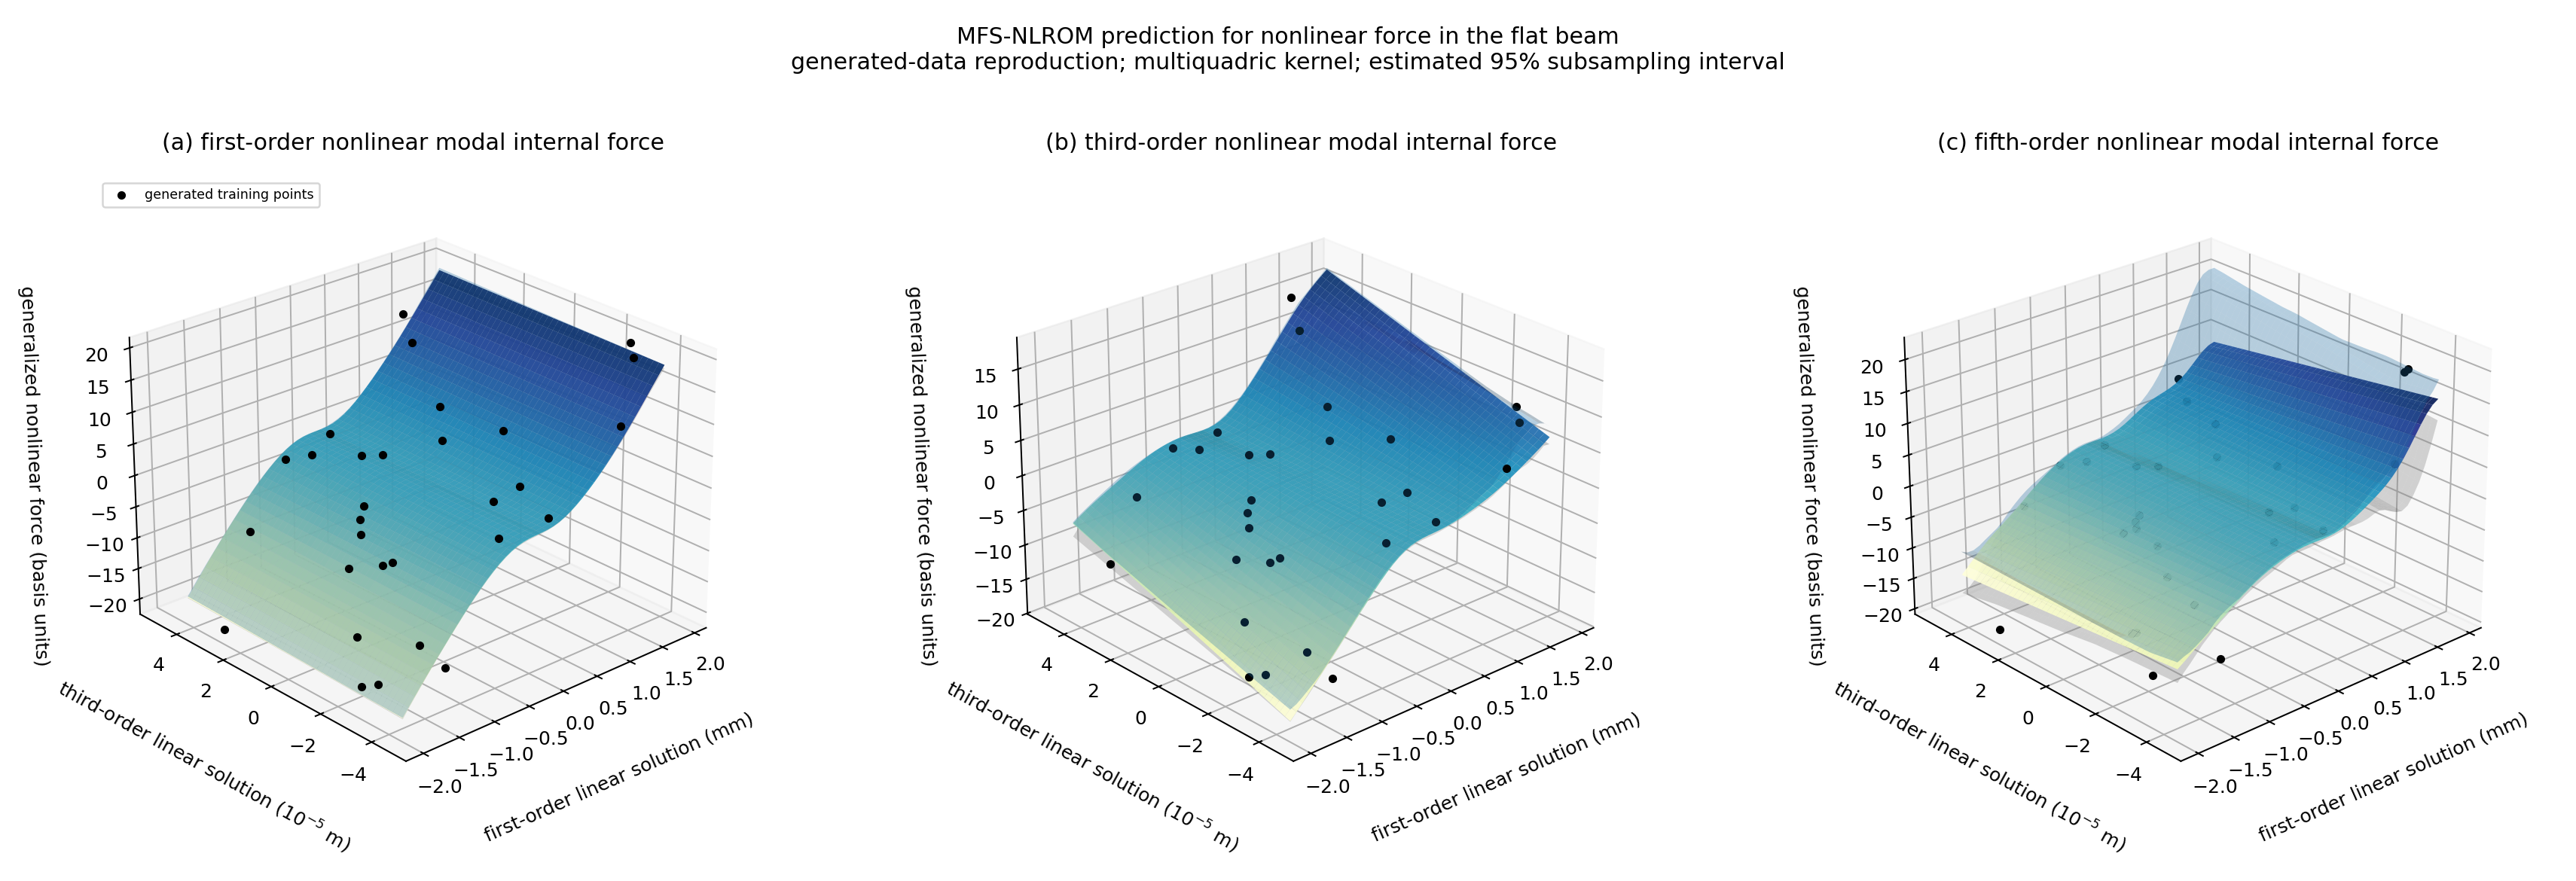
\includegraphics[width=0.8\linewidth]{figures/ch14r/mfs_surfaces.png}
\caption{Fitted nonlinear modal force of modes 1, 3 and 5 (multiquadric kernel) over the linear amplitudes of modes 1 and 3; the black dots are the OLHS training points of this run, and the shaded band is an improvised $95\,\%$ subsampling interval. The mode-5 input is held at its training mean.}\label{fig:vf-mfs-surf}
\end{figure}

\begin{table}[tbp]
\centering\footnotesize
\caption{Static accuracy ($R^2$ against nonlinear finite elements, unseen samples) of the flat beam.}\label{tab:vf-mfs-static}
\begin{tabular}{@{}lrr@{}}
\toprule
Model & This work & Publication\\
\midrule
Multi-fidelity, multiquadric & 0.9982 & 0.9997\\
Multi-fidelity, cubic & 0.9889 & 0.9996\\
Multi-fidelity, thin-plate spline & 0.9860 & 0.9998\\
Multi-fidelity, Gaussian & 0.9968 & 0.9853\\
ICE polynomial & 1.0000 & 1.0000\\
\bottomrule
\end{tabular}
\end{table}

\emph{Free decay.} \Cref{tab:vf-mfs-decay} compares the tip response over 190~ms for two initial conditions: case~(a) releases the beam from the static state of the strongest negative load ($q_{\rm nl}/q_{\rm l}\approx0.5$, strongly hardening); case~(b) starts from half a thickness of the first mode shape. The Newton treatment of the implicit force and the polynomial baseline lie on the full-order curve (\Cref{fig:vf-mfs}b). The lagged-force path of the library translates the initial condition from $q_{\rm nl}$ to $q_{\rm l}$ with a single Picard refinement and lands $23\,\%$ short in case~(a), which gives $R^2<0$; the Newton path corrects this exactly. The reconstructed predictor--corrector scheme diverges in both cases.

\begin{table}[tbp]
\centering\footnotesize
\setlength{\tabcolsep}{4pt}
\caption{Free-decay accuracy ($R^2$ of the tip response against nonlinear finite elements), flat beam.}\label{tab:vf-mfs-decay}
\begin{tabular}{@{}lrrrrr@{}}
\toprule
Case & MFS, Newton & ICE & MFS, lagged force & MFS, predictor--corrector & Publication (MFS / ICE)\\
\midrule
(a) $F_{\rm nl}(0)=-2068$ Pa & 0.9971 & 0.9981 & $-0.89$ & $-853$ & 0.9837 / $-0.63$\\
(b) $q_{\rm nl}(0)=0.5\,t\,\phi_1$ & 0.9898 & 0.9987 & 0.9907 & $-3141$ & 0.9836 / 0.9008\\
\bottomrule
\end{tabular}
\end{table}

\emph{Sample size.} The unseen $R^2$ against the number of training samples (\Cref{fig:vf-mfs-samples}) is $0.844$, $0.986$, $0.9994$ and $1.0000$ for $N=9$, $15$, $30$ and $60$: substantial improvement at small $N$, and a knee near the publication's recommended $N=10n$.

\begin{figure}[tbp]
\centering
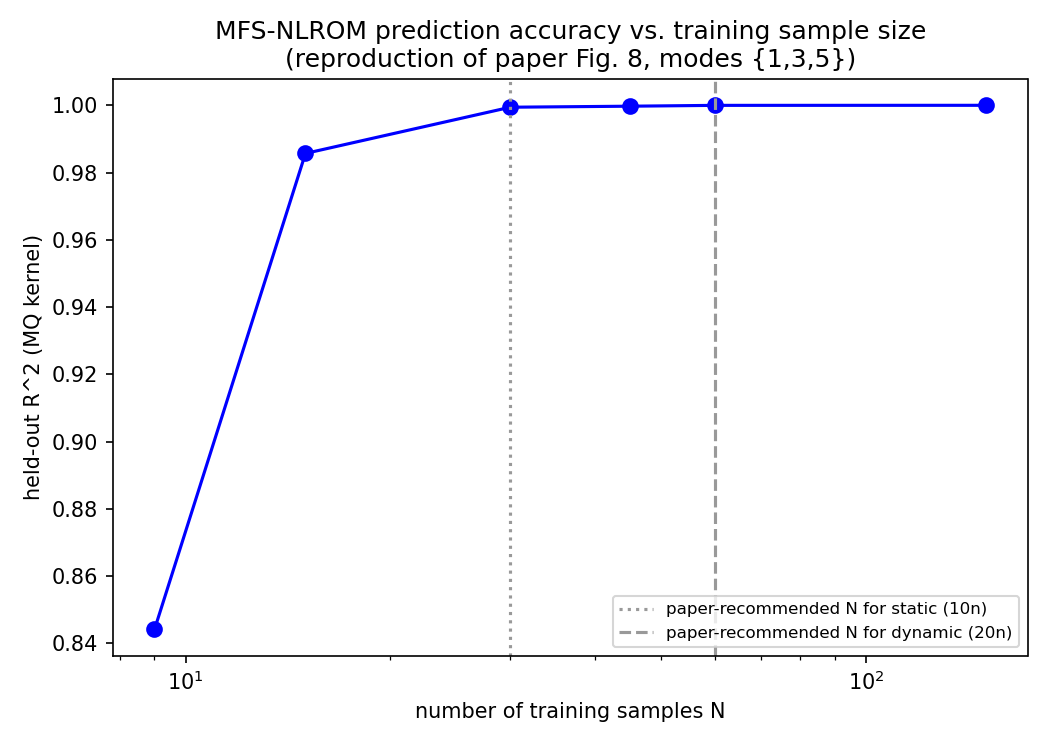
\includegraphics[width=0.6\linewidth]{figures/ch14r/mfs_samples.png}
\caption{$R^2$ on unseen samples against the number of training samples, flat beam.}\label{fig:vf-mfs-samples}
\end{figure}

\begin{figure}[tbp]
\centering
\includegraphics[width=1.0\linewidth]{figures/ch14_mfs.pdf}
\caption{Flat beam of \citet{he2023mfsnlrom}. (a) Centre displacement over $\pm2000$~Pa: nonlinear FE, multi-fidelity surrogate and ICE ($R^2=\cvfMfsRtwoMfs$ and $\cvfMfsRtwoIce$ against FE). (b) Free decay of the first modal coordinate ($R^2=\cvfMfsDecayA$ for case a and $\cvfMfsDecayB$ for case b). (c) Backbone by harmonic balance against FE free vibration; largest frequency error $\cvfMfsBackErr$ over a hardening of $\cvfMfsHardening$ above the linear frequency. One surrogate evaluation takes \cvfMfsTmfs{}~s against \cvfMfsTfe{}~s for FE, a ratio of \cvfMfsSpeed.}\label{fig:vf-mfs}
\end{figure}

\emph{Backbone.} \Cref{tab:vf-mfs-back} gives the frequency of the first nonlinear mode against its amplitude. The beam hardens by about $22\,\%$ over the range; the largest error against free vibration of the full model is $0.96\,\%$ for the surrogate and $0.87\,\%$ for the baseline.

\begin{table}[tbp]
\centering\footnotesize
\caption{Backbone of the flat beam; linear frequency 78.97~Hz.}\label{tab:vf-mfs-back}
\begin{tabular}{@{}lrrrrrr@{}}
\toprule
$q_1$ ($\times10^{-5}$) & 2.05 & 2.96 & 3.86 & 4.76 & 5.67 & 6.57\\
\midrule
FE free vibration (Hz) & 80.56 & 83.08 & 85.96 & 88.50 & 93.00 & 96.27\\
MFS-NLROM (Hz) & 81.33 & 83.22 & 85.86 & 89.14 & 92.94 & 97.18\\
ICE (Hz) & 80.96 & 83.04 & 85.76 & 89.07 & 92.87 & 97.10\\
\bottomrule
\end{tabular}
\end{table}

\subsection*{Results: wing}

\emph{Reconstructed geometry and modes.} The first four frequencies of the reconstructed wing are 16.8, 84.0, 221.8 and 256.4~Hz with ten-node tetrahedra and 16.7, 83.0, 216.7 and 251.6~Hz with twenty-node hexahedra, against 15, 73, 191 and 223~Hz in the publication (\Cref{fig:vf-mfs-wing}a). The two meshes agree to $1$--$2\,\%$ on every mode, which is an independent confirmation of the converged answer. Clamping at the 50~mm end matches the publication to within $11$--$16\,\%$ uniformly on every mode, whereas clamping at the other end gives a ragged $7$--$45\,\%$ spread; a uniform spread is the signature of the right boundary condition, although it does not prove the publication's fixture, and the remaining gap is plausibly root-fixture stiffness that the schematic cannot specify.

\emph{Why the shell is the reference.} The wing is 1.15~mm thick and the solid model has one element layer through that thickness at an in-plane size of 90~mm, an aspect ratio near 78:1. The Green--Lagrange strain
\begin{equation}\label{eq:mfs-gl}
\mathbf E=\tfrac12\left(\nabla\mathbf u+\nabla\mathbf u^{T}+\nabla\mathbf u^{T}\nabla\mathbf u\right)
\end{equation}
is quadratic in displacement \emph{gradients}, and gradients across the thin layer are amplified: for the softest eigenmode the nonlinear internal force exceeds the linear prediction by a factor of 70 at 1~\textmu m of displacement (a rotation of about $0.0004^\circ$), scaling as $u^2$ against the linear term's $u^1$. A too-large load or time increment, rounding from the mesh condition number (about $2\times10^{11}$) and genuine large-rotation physics were each ruled out by direct tests; in-plane refinement barely changes the effect, and more layers through the thickness make it worse ($3957\times$ to $7128\times$ from one to four layers). A shell element never discretises the thickness, and its force ratio stays flat over six orders of magnitude of amplitude.

The choice of shell element matters as well. \Cref{tab:vf-mfs-shell} shows the ratio $q_{{\rm nl},1}/q_{{\rm l},1}$ for pure mode-1 loads (1 means no nonlinearity): the corotational shell shows no geometric stiffening even at a tip displacement of 46~mm, so an early run that used it fitted numerical noise and had a deeply negative unseen $R^2$; \texttt{Shell4Director} stiffens as it should and is the reference.

\begin{table}[tbp]
\centering\footnotesize
\caption{Ratio $q_{{\rm nl},1}/q_{{\rm l},1}$ for mode-1 tip loads of a given multiple of the thickness.}\label{tab:vf-mfs-shell}
\begin{tabular}{@{}lrrrr@{}}
\toprule
Tip load (thickness) & 3 & 10 & 20 & 40\\
\midrule
\texttt{Shell4MITCCorotational} & 1.00000 & 1.00000 & 0.99998 & 0.99992\\
\texttt{Shell4Director} & 0.99976 & 0.99765 & 0.99100 & 0.96780\\
\bottomrule
\end{tabular}
\end{table}

\begin{figure}[tbp]
\centering
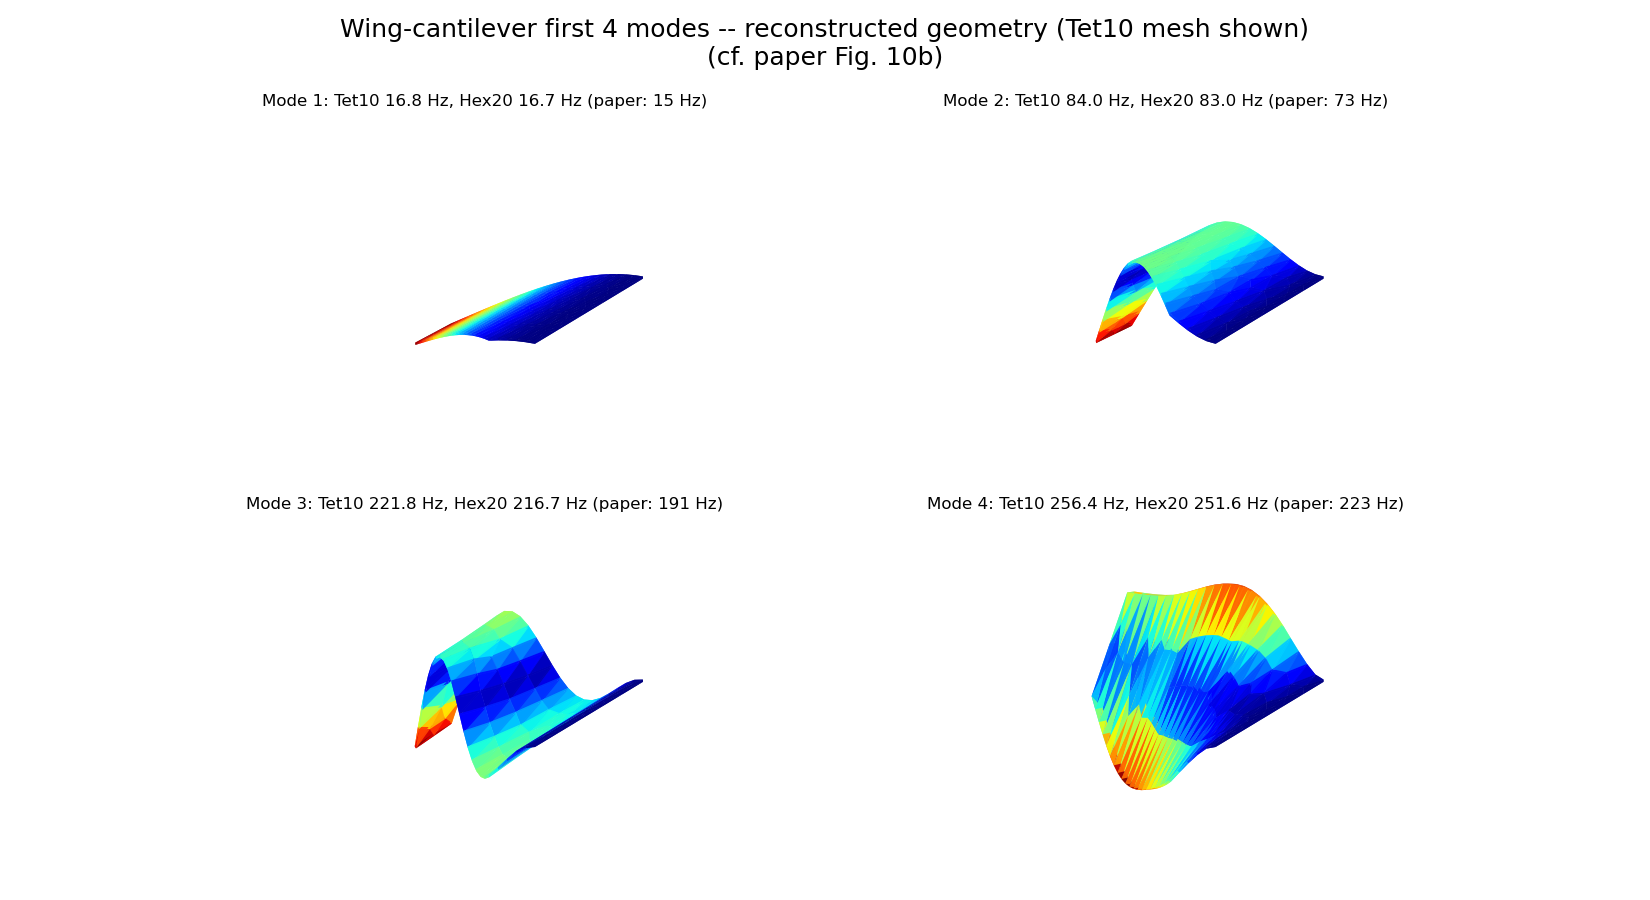
\includegraphics[width=0.8\linewidth]{figures/ch14r/mfs_wing_modes.png}
\caption{First four modes of the reconstructed wing (ten-node tetrahedron mesh; colour is displacement magnitude).}\label{fig:vf-mfs-wing}
\end{figure}

\emph{Static tip sweep.} \Cref{fig:vf-mfs-wing2} (left) shows the tip displacement against the mode-1 linear amplitude. Both reduced models give a sweep $R^2$ of $1.0000$, but the nonlinear part is only $2.6$--$3.8\,\%$ of the linear modal force at these amplitudes and the linear finite element alone scores $0.9993$, so the discriminating number is the $R^2$ of the nonlinear deviation $w-w_{\rm lin}$: $0.984$ for the surrogate (Gaussian kernel, unseen force $R^2=0.974$; MQ $0.915$, cubic $0.909$, TPS $0.875$) and $0.9999$ for the polynomial baseline (unseen $0.997$). The polynomial wins because the true force is close to the quadratic-plus-cubic form it assumes; the surrogate shows a $-0.09$~mm zero-load offset from the Gaussian fit.

\begin{figure}[tbp]
\centering
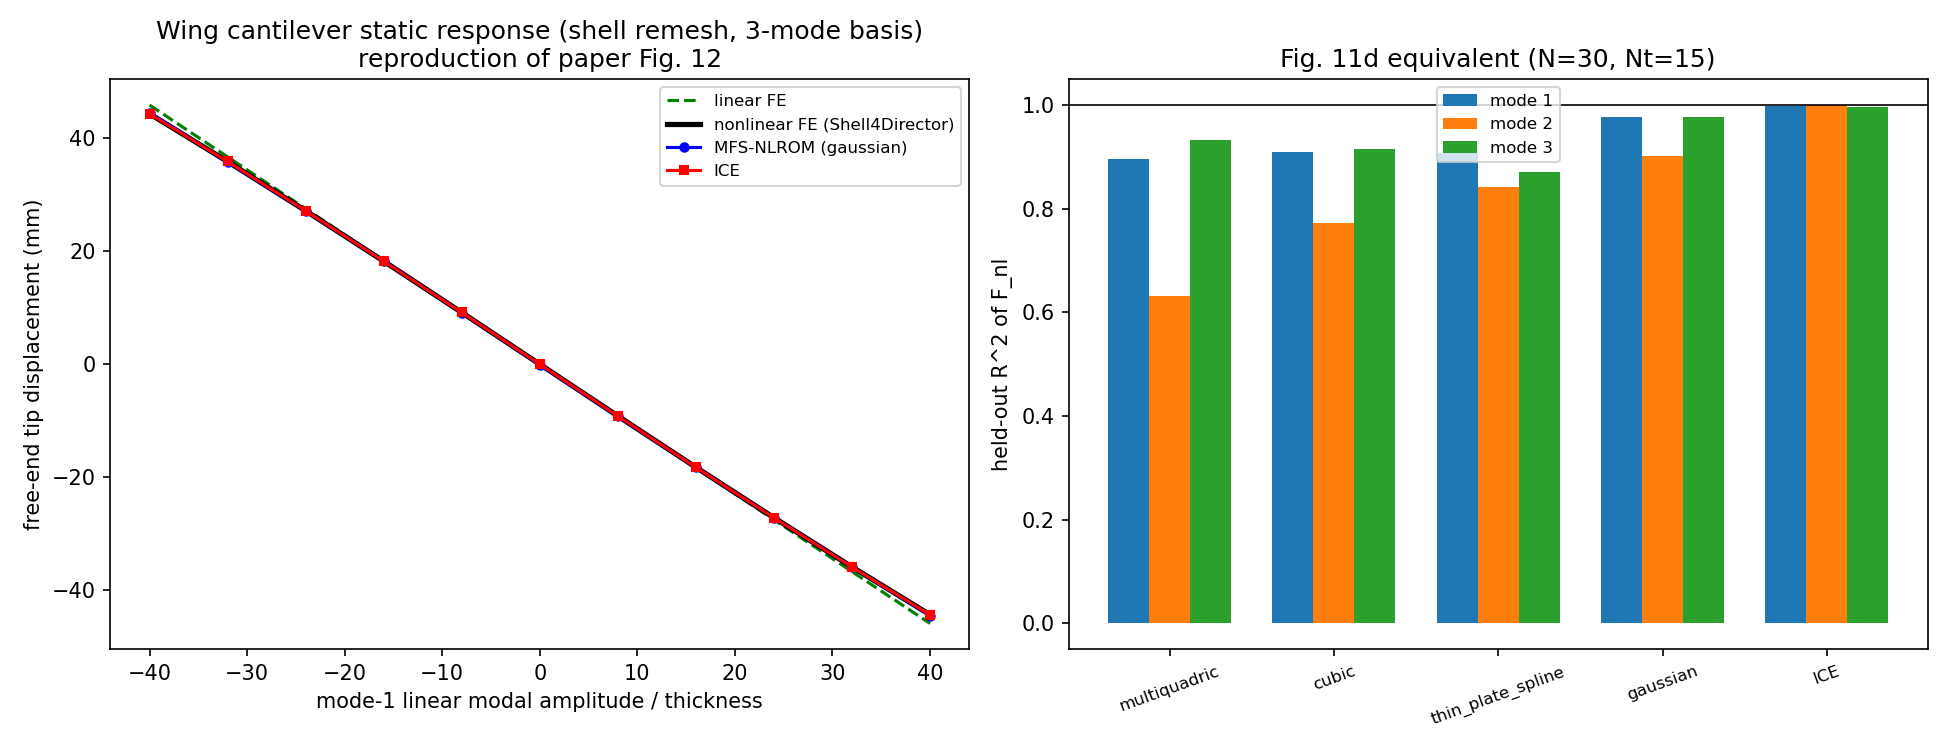
\includegraphics[width=0.8\linewidth]{figures/ch14r/mfs_wing_sweep.png}
\caption{Shell wing, static tip-load sweep. Left: tip displacement against the mode-1 linear amplitude for nonlinear FE, linear FE, MFS-NLROM (Gaussian) and ICE. Right: unseen $R^2$ of $F_{\rm nl}$ per mode and kernel.}\label{fig:vf-mfs-wing2}
\end{figure}

\emph{Free decay.} \Cref{tab:vf-mfs-wdecay} gives the shell wing's tip response over about two periods ($\Delta t=2$~ms, 60 steps, about 22~mm amplitude). Case~(b) is an impulsive start with a mode-1 velocity and zero displacement, because a mode-shape displacement is not an admissible initial condition for a Green--Lagrange shell at this amplitude. Every scheme reaches $R^2\ge0.9998$, including the predictor--corrector that diverged on the beam. One full-order run takes about 2\,700~s, so the speed-ups of the table (from $1.2\times10^{4}$ to $5\times10^{5}$) are against that.

\begin{table}[tbp]
\centering\footnotesize
\caption{Free decay of the shell wing: $R^2$ of the tip displacement and, in brackets, the speed-up over finite elements.}\label{tab:vf-mfs-wdecay}
\begin{tabular}{@{}lllll@{}}
\toprule
Case & MFS, Newton & ICE & MFS, lagged force & MFS, predictor--corrector\\
\midrule
(a) released from static equilibrium & 0.9999 (29\,332$\times$) & 0.9999 (54\,316$\times$) & 0.9999 (257\,572$\times$) & 0.9998 (450\,026$\times$)\\
(b) impulsive, mode-1 velocity & 0.9999 (12\,364$\times$) & 0.9999 (65\,841$\times$) & 0.9999 (272\,622$\times$) & 0.9999 (501\,086$\times$)\\
\bottomrule
\end{tabular}
\end{table}

\emph{Backbone.} \Cref{tab:vf-mfs-wback} gives the backbone of mode 1 (linear frequency $16.668$~Hz). Both reduced models capture the hardening trend but overpredict it by about a factor of two (at 31.3 thicknesses the shift above linear is $+0.89\,\%$ and $+0.82\,\%$ against $+0.36\,\%$ for finite elements); the whole effect is about $0.4\,\%$ of the frequency, so the maximum errors ($0.53\,\%$ and $0.45\,\%$) are small in absolute terms.

\begin{table}[tbp]
\centering\footnotesize
\caption{Backbone of the shell wing, mode 1.}\label{tab:vf-mfs-wback}
\begin{tabular}{@{}lrrrr@{}}
\toprule
Amplitude (thickness) & 8.0 & 15.9 & 23.7 & 31.3\\
\midrule
FE (Hz) & 16.672 & 16.684 & 16.704 & 16.728\\
MFS-NLROM (Hz) & 16.657 & 16.692 & 16.748 & 16.816\\
ICE (Hz) & 16.677 & 16.703 & 16.746 & 16.803\\
\bottomrule
\end{tabular}
\end{table}

\begin{figure}[tbp]
\centering
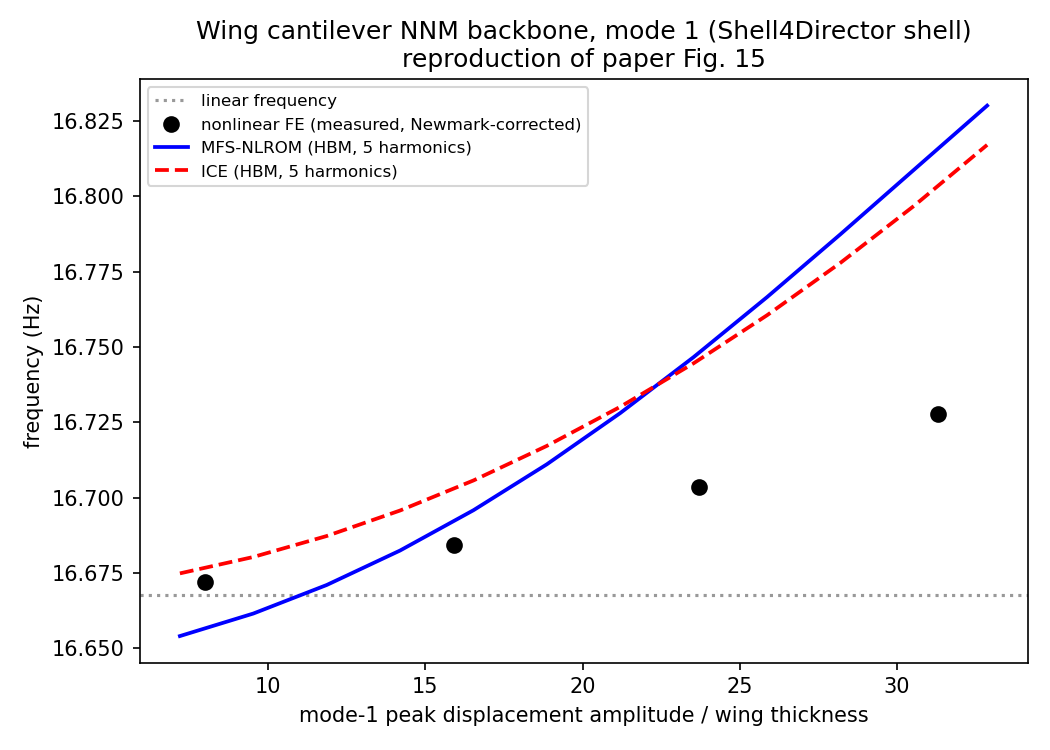
\includegraphics[width=0.6\linewidth]{figures/ch14r/mfs_wing_backbone.png}
\caption{Backbone of mode 1 of the shell wing: harmonic balance with five harmonics for the reduced models, free vibration from static equilibria for the full-order model.}\label{fig:vf-mfs-wback}
\end{figure}

The solid wing model gives unseen $R^2$ of $0.780$ (surrogate, thin-plate spline) and $1.000$ (polynomial), a tip sweep of $0.9987$ and $1.0000$, and free decay of $0.9646$ and $1.0000$; its finite element reference fails to converge at large amplitude, so only one of three backbone points and a truncated window of case~(b) could be compared. The solid results are therefore secondary and are not used as evidence.

\subsection*{Comparison with the publication}

\begin{table}[tbp]
\centering\footnotesize
\caption{Claims of \citet{he2023mfsnlrom} and the outcome of the reproduction.}\label{tab:vf-mfs-cmp}
\begin{tabularx}{\linewidth}{@{}>{\raggedright\arraybackslash}p{4.1cm} >{\raggedright\arraybackslash}X >{\raggedright\arraybackslash}p{2.3cm}@{}}
\toprule
Claim & This work & Outcome\\
\midrule
Linear modes of the beam (Fig.~4) & within $0.15\,\%$ & reproduced\\
Nonlinear-force surfaces (Fig.~5) & axis ranges and shape match; training points unpublished & reproduced (shape)\\
Static accuracy by kernel (Table~2) & MQ and ICE agree; ranking of other kernels differs & partly\\
Pressure sweep and speed ordering (Fig.~6, Table~4) & $R^2=1.0000$; MFS $\gg$ ICE $\gg$ FE & reproduced\\
Free decay (Fig.~7, Table~3) & $R^2=0.990$--$0.997$ (publication 0.984); ICE failure ($-0.63$) not seen & reproduced; ICE failure not\\
Sample-size sensitivity (Fig.~8) & saturates near $N=10n$ & reproduced\\
Backbone (Fig.~9) & error $<1\,\%$ over a $22\,\%$ hardening & reproduced\\
Wing static, dynamic, backbone (Figs.~12, 15) & shell: $R^2=1.0000$, $0.9999$, error $\le0.53\,\%$ & reproduced on the shell\\
Hammer test (Figs.~13, 14) & measured signals cannot be recovered from the publication & not reproduced\\
\bottomrule
\end{tabularx}
\end{table}

\subsection*{Missing equations and an early failure}

The equations for the training-load scaling and the time-integration scheme of the publication did not survive text extraction from the PDF. The load scaling is structurally confirmed by the appendix of the publication, but its iterative calibration loop is not implemented; a fixed target-fraction range tuned to the axes of its Fig.~5 is used instead, and the time-integration scheme is a reconstruction that diverges on the flat beam, which is why a Newton solve of the same relation is used. The publication states no damping ratio, so $1\,\%$ modal Rayleigh damping is assumed in every dynamic case. The full-order backbone is obtained by free vibration and period measurement, not by the publication's multi-harmonic-balance solver on the full model. The wing planform is digitised, its frequencies lie $11$--$16\,\%$ from the publication's, and its training sizes are reduced. Both reduced models are valid only inside their training range, and the publication's hammer test cannot be rebuilt. Finally, the polynomial baseline matches or exceeds the surrogate in accuracy on these smooth, weakly nonlinear problems, so the benefit measured here is speed and generality, not accuracy.

An early failure of the flat-beam run (sweep $R^2=0.54$, free-decay $R^2=-1.00$, overflow of the baseline) came from the author's driver, which scanned the mode-shape peaks over rotation degrees of freedom and so made the training amplitudes 13 to 72 times too small. After the correction the sweep gives $R^2=1.000$ for both models; the sample-size curve at $N=9$ changed from 0.995 to 0.844 and the backbone span from $79.0$--$79.3$ to $80.6$--$96.3$~Hz.

\section{Hybrid modal ROM from static solves}\label{sec:vf-hyrom}

\subsection*{Concept and purpose}

\citet{yang2019hybrid} train a modal reduced model of a geometrically nonlinear structure from \emph{static} solves of the full-order model (implicit condensation) and then use it for forced transient response. The full nonlinear internal force is replaced by a linear part plus a nonlinear modal force that is a polynomial in the modal coordinates, and the coefficients are fitted by least squares to static data. The study tests two structures of different character: a cantilever plate with a hole, whose free edge lets in-plane motion occur, and a hinged shallow cylindrical panel, whose edges are fixed in space. The test of the method is not the static fit, which is easy, but whether the model predicts a strongly nonlinear forced transient and, as an added check that a transient can hide, the free-vibration backbone.

The finite element models use \anchor{fea_engine.elements.Shell4Director} and \anchor{fea_engine.elements.Shell4MITC}; the reduced model is the polynomial modal model of \rom{} (\anchor{rom_engine.PolynomialModalROM}) with the Newmark integrator for reduced models and the Koiter--Newton static solver of \fea{} for the panel.

\subsection*{Mathematics as implemented}

The semi-discrete full-order model with $n$ free degrees of freedom is
\begin{equation}\label{eq:hy-fom}
\mathbf M\ddot{\mathbf u}+\mathbf C\dot{\mathbf u}+\mathbf f_{\rm int}(\mathbf u)=\mathbf f_{\rm ext}(t),
\end{equation}
with the linear tangent stiffness $\mathbf K=\partial\mathbf f_{\rm int}/\partial\mathbf u|_{\mathbf 0}$ and mass-normalised modes $\mathbf V^{T}\mathbf M\mathbf V=\mathbf I$, $\mathbf K\boldsymbol\phi_r=\lambda_r\mathbf M\boldsymbol\phi_r$, $\lambda_r=(2\pi f_r)^2$. Projecting $\mathbf u\approx\mathbf V\mathbf q$ gives the $N$-degree-of-freedom model
\begin{equation}\label{eq:hy-rom}
\ddot{\mathbf q}+\mathbf C_r\dot{\mathbf q}+\boldsymbol\Lambda\mathbf q+\mathbf F_{\rm nl}(\mathbf q)=\mathbf V^{T}\mathbf f_{\rm ext}(t),\qquad\boldsymbol\Lambda=\operatorname{diag}(\lambda_r).
\end{equation}

\emph{Identification.} For training sample $i$ a modal force $\hat{\mathbf f}_i$ is drawn, the physical load is $\mathbf F_i=\mathbf M\mathbf V\hat{\mathbf f}_i$ (so $\mathbf V^{T}\mathbf F_i=\hat{\mathbf f}_i$ exactly), and the nonlinear static problem $\mathbf f_{\rm int}(\mathbf u_i)=\mathbf F_i$ is solved. Projection gives
\begin{equation}\label{eq:hy-id}
\mathbf q_i^{\rm nl}=\mathbf V^{T}\mathbf M\mathbf u_i,\qquad\mathbf F_{{\rm nl},i}=\hat{\mathbf f}_i-\boldsymbol\Lambda\mathbf q_i^{\rm nl},
\end{equation}
and each component is fitted by ordinary least squares to the quadratic-plus-cubic form
\begin{equation}\label{eq:hy-nash}
F_{{\rm nl},r}(\mathbf q)=\sum_{i\le j}B_r(i,j)\,q_iq_j+\sum_{i\le j\le k}A_r(i,j,k)\,q_iq_jq_k,
\end{equation}
which has $N(N+1)/2+N(N+1)(N+2)/6$ terms (7 for $N=2$, 83 for $N=6$); the number of samples is $\max(\lceil1.3\,n_{\rm terms}\rceil,15)$ or more.

\emph{Training loads.} The target peak displacement of mode $r$ is drawn by optimal Latin-hypercube sampling in a range of $a_r$ thicknesses, $Q^{\max}_r=a_rh$, and the modal force follows as $\hat f_r=(Q_r^{\max}/\phi_r^{\max})\lambda_r$. The ranges are signed (push and pull) because the transient swings through both signs.

\emph{Time integration.} Newmark-$\beta$ ($\beta=\tfrac14$, $\gamma=\tfrac12$) with the nonlinear force treated implicitly, by \texttt{newton} (Newton on the reduced residual with the polynomial Jacobian), \texttt{fixed\_point} (four Picard sweeps; it matches \texttt{newton} to printed precision at the time steps used) or \texttt{sign\_deviation} (the predictor--corrector of \citet{he2023mfsnlrom}, Eq.~32). The last applies $\operatorname{sign}(\ddot q)\,[F_{\rm nl}(t{+}\Delta t)-F_{\rm nl}(t)]$; for modes with negative acceleration this reverses the correction, the error propagation is $2\mathbf I-\mathbf A$ instead of $\mathbf A$ with $\mathbf A=-\mathbf J_{\rm nl}\mathbf K_{\rm eff}^{-1}$, and it diverges on the panel for every mode set, so it is not used.

\emph{Metrics.} The transient error is
\begin{equation}\label{eq:hy-err}
\varepsilon=\frac{\max_t|w_{\rm ROM}(t)-w_{\rm FOM}(t)|}{\max_t|w_{\rm FOM}(t)|}.
\end{equation}
For the panel a projection baseline is also reported: the full-order history projected on the retained modes and reconstructed, the truncation-only floor of any model of that size. The backbone test releases mode~1 from a static state, oscillates undamped and measures the frequency against the linear one, giving $f/f_{\rm lin}$ against amplitude; agreement of the backbone shows that $\mathbf F_{\rm nl}$ is right \emph{dynamically}, not only statically.

\subsection*{Geometry and mesh}

Case~1 is a cantilever plate of aluminium, $1\times0.2\times0.01$~m, with a hole of radius $0.02$~m at mid-length, clamped at one end (7 nodes) and loaded by a 500~N, 2.5~Hz point force at the midpoint of the free end (\Cref{fig:vf-hy-mesh1}). The mesh has 204 nodes, 168 elements and 1224 degrees of freedom (the publication's has 2394). Case~2 is a shallow cylindrical panel of $R=2540$~mm, $L=508$~mm, $t=12.5$~mm and half-angle $0.1$~rad, with $E=3102.75$~MPa, $\nu=0.3$ and $\rho=5\times10^{-7}$~kg/mm$^3$, hinged on all four edges (translations fixed, rotations free) and loaded at the crown by 5000~N at 2.5~Hz (\Cref{fig:vf-hy-geom2}). The package has no curved-shell mesher, so a structured $10\times10$ grid in $(x,\theta)$ is mapped onto the cylinder (100 elements, 121 nodes, 726 degrees of freedom), and the crown load is spread over a $3\times3$ patch of nodes because a single-node load on this coarse mesh dimples locally too early.

\begin{figure}[tbp]
\centering
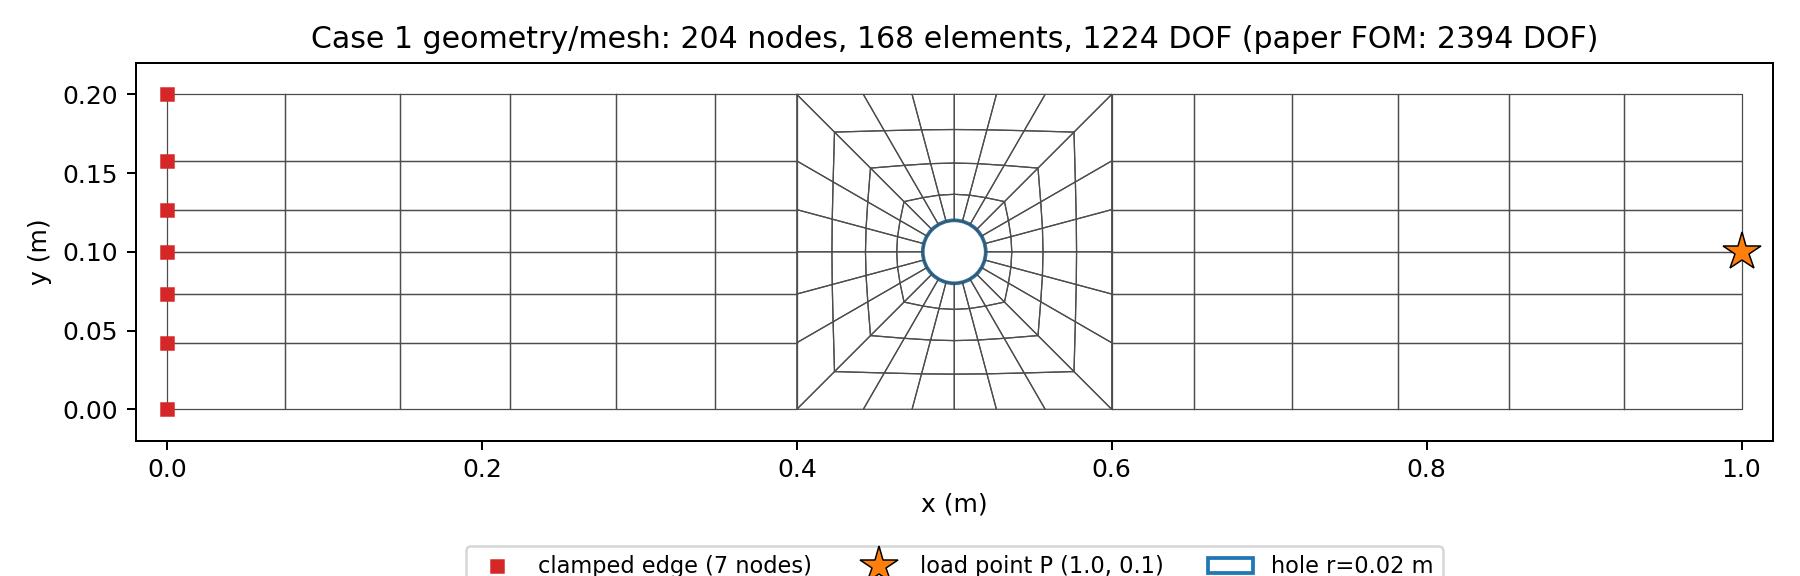
\includegraphics[width=0.8\linewidth]{figures/ch14r/hy_c1_mesh.png}
\caption{Case 1: plate with a hole. Mesh with 204 nodes and 168 elements (1224 degrees of freedom), clamped edge (red squares), load point (star) and the hole.}\label{fig:vf-hy-mesh1}
\end{figure}

\begin{figure}[tbp]
\centering
\includegraphics[width=0.95\linewidth]{figures/ch14_geom_hyrom.pdf}
\caption{Case 2: shallow cylindrical panel, drawn from the dimensions of the report. (a) The $10\times10$ mesh on the cylinder, hinged edge nodes, free nodes and the $3\times3$ crown load patch. (b) Section through the crown line.}\label{fig:vf-hy-geom2}
\end{figure}

\begin{table}[tbp]
\centering\footnotesize
\caption{Set-up of the two cases.}\label{tab:vf-hy-setup}
\begin{tabularx}{\linewidth}{@{}>{\raggedright\arraybackslash}p{3.0cm} >{\raggedright\arraybackslash}X >{\raggedright\arraybackslash}X@{}}
\toprule
Item & Case 1: plate with hole & Case 2: cylindrical panel\\
\midrule
Structure & cantilever $1\times0.2\times0.01$ m, hole $r=0.02$ m, aluminium & hinged panel $R=2540$, $L=508$, $t=12.5$ mm\\
Load & 500 N point load, 2.5 Hz & 5000 N crown load, 2.5 Hz\\
Size (this work / publication) & 1224 / 2394 dofs & 726 dofs\\
Training & 15 OLHS samples, signed ranges $q_1\in[-0.25,0.25]$, $q_2\in[-0.008,0.008]$; incremental Newton in 20 steps & 15 to 101 samples by mode set; Koiter--Newton ($\approx41$ s each)\\
Mode choice & modes 1, 2 & by projection of the load: 1, 6, 5, 9, 17, 16 (set sizes 2, 2, 3, 4, 6 as published, not the same hand-picked modes)\\
Time step & $\Delta t=0.005$ s, 200 steps & as in the publication\\
\bottomrule
\end{tabularx}
\end{table}

\subsection*{Results: verification of the full-order model}

\emph{Modes of case 1.} The four lowest frequencies are 8.35, 52.45, 81.60 and 150.49~Hz against 8.33, 51.98, 79.38 and 146.20~Hz in the publication, differences of $0.3$, $0.9$, $2.8$ and $2.9\,\%$ (\Cref{fig:vf-hy-modal}). The growth of the error with the mode number is plausibly the coarser mesh, which was not tested. For case~2 the modes 1 to 8 are 5.93, 9.63, 10.49, 15.40, 19.91, 20.41, 25.40 and 25.62~Hz; the publication gives no frequency table.

\begin{figure}[tbp]
\centering
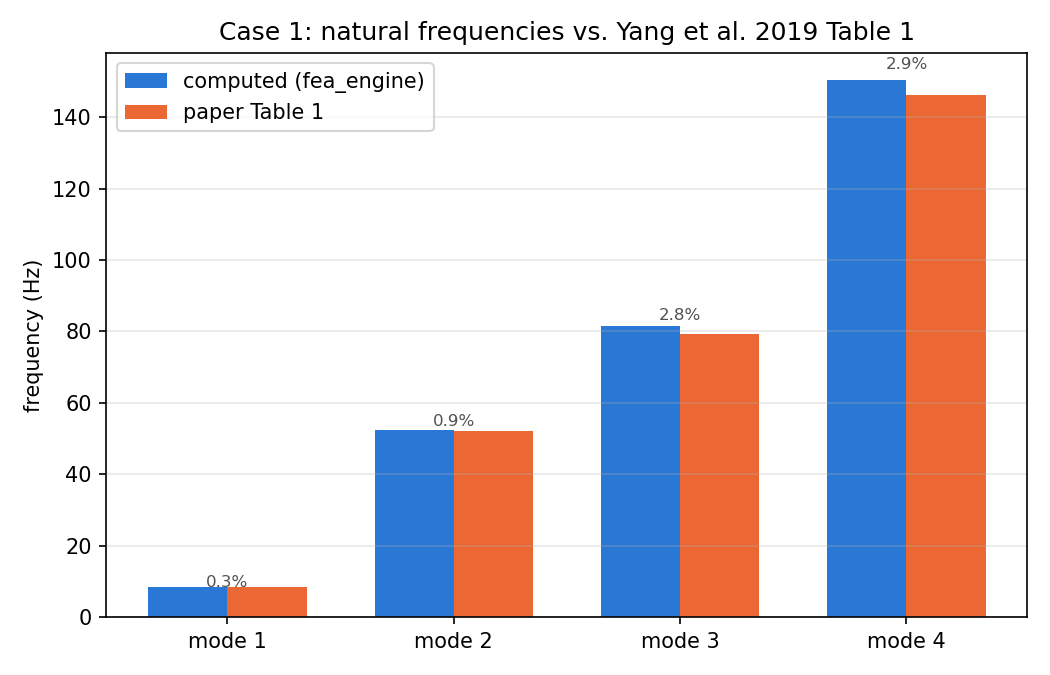
\includegraphics[width=0.6\linewidth]{figures/ch14r/hy_c1_modal.png}
\caption{Case 1: natural frequencies against the publication's Table~1.}\label{fig:vf-hy-modal}
\end{figure}

\emph{The element's geometric nonlinearity.} A first version of the case-1 model gave a nearly linear transient. The cause was the element, not the integrator: tested on a clamped strip with a tip load against the exact elastica, the shell element with a ``moderate'' curvature measure gave a tip-deflection ratio of $1.0005$ where the elastica gives $0.8725$, i.e.\ no stiffening at all. With the Green--Lagrange curvature measure of \texttt{Shell4Director} the ratio is $0.8729$ (\Cref{fig:vf-hy-elastica}). The narrow strips follow the elastica in stiffening and tip foreshortening; the plate-width strip deviates in stiffening and tip rotation, and the narrow strip at 40 elements diverges at the first load step, a separate robustness issue that remains open. The change moves the panel results by at most $0.15\,\%$ in displacement.

\begin{figure}[tbp]
\centering
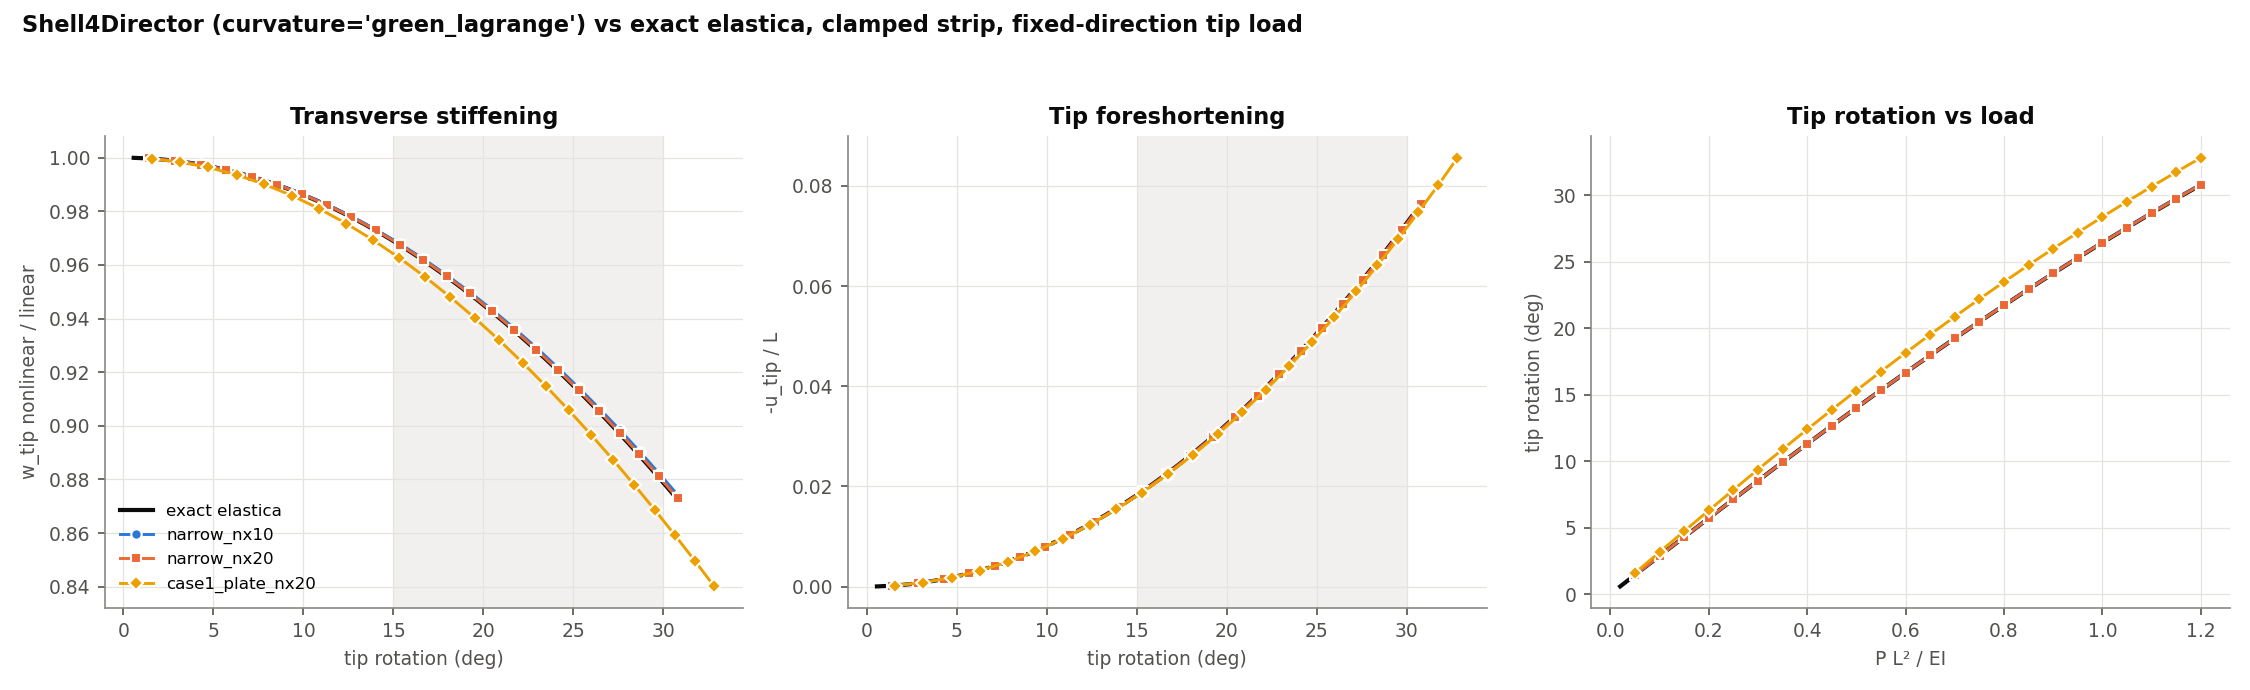
\includegraphics[width=0.8\linewidth]{figures/ch14r/hy_elastica.png}
\caption{Element check on a clamped strip against the exact elastica, for strips of increasing width and mesh density.}\label{fig:vf-hy-elastica}
\end{figure}

\subsection*{Results: case 1, plate with hole}

\emph{Full-order transient.} Over 200 steps of $\Delta t=0.005$~s the nonlinear response differs from the linear one by $12.8\,\%$ of the peak and the gap grows over the cycles, the signature of the publication's Fig.~6: the peak is $0.1910$~m nonlinear against $0.1969$~m linear (hardening). The publication reports roughly $20$--$40\,\%$ locally, so the magnitude is smaller here; the coarser mesh is a candidate cause that was not investigated.

\begin{figure}[tbp]
\centering
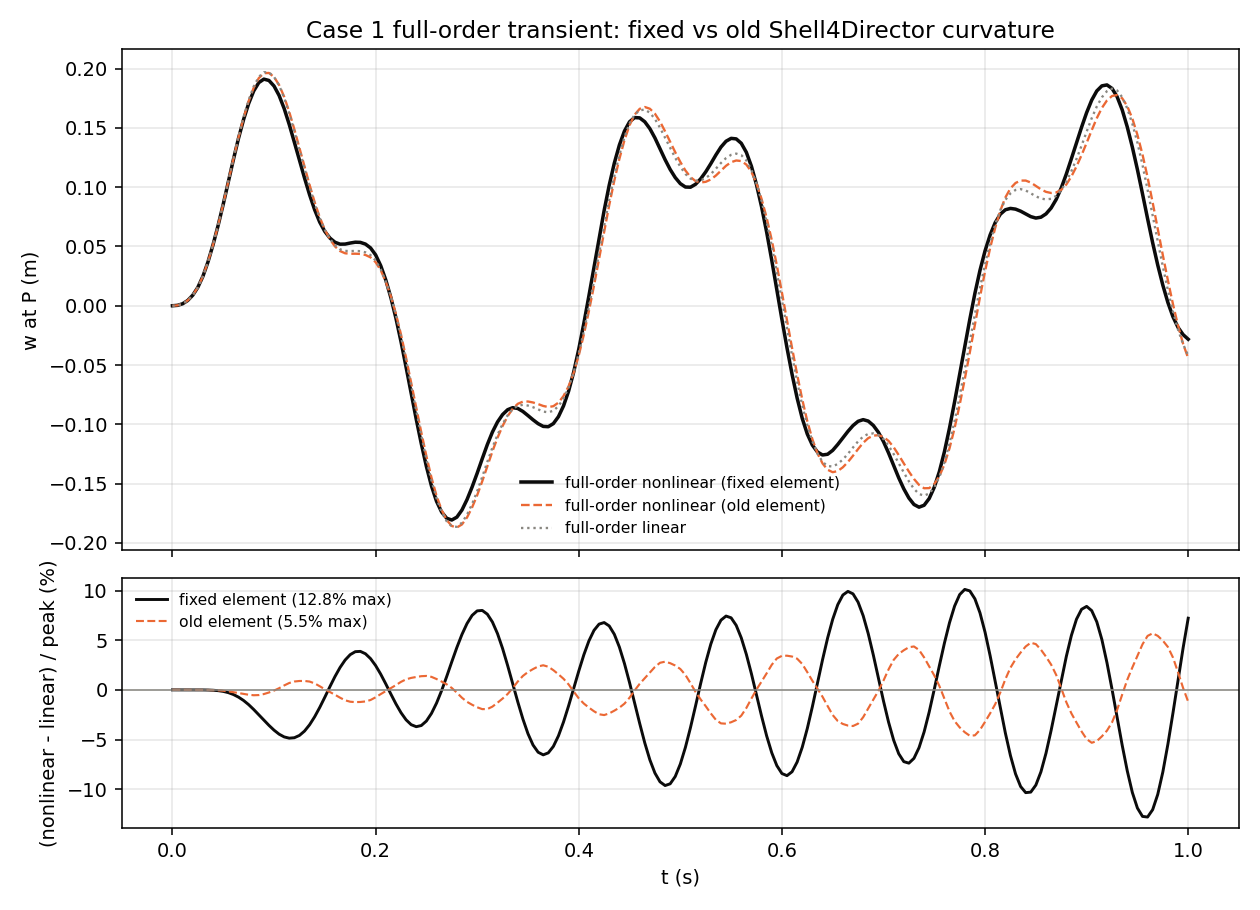
\includegraphics[width=0.8\linewidth]{figures/ch14r/hy_c1_fom.png}
\caption{Case 1: full-order transient, nonlinear (Green--Lagrange curvature) against linear.}\label{fig:vf-hy-c1fom}
\end{figure}

\emph{Static training and ROM transient.} The cubic fit of the 15 signed samples has a maximum training error of $0.71\,\%$; the static hardening in $q_1$ is $0.998$ (nonlinear over linear) at $q_1=0.05$ and $0.951$ at $q_1=0.25$. An earlier one-sided training range ($q_1\in[0.004,0.020]$) needed a tenfold extrapolation and gave $20\,\%$ error, which, and not the integrator, was the cause (\texttt{fixed\_point} and \texttt{newton} agree). \Cref{tab:vf-hy-c1} gives the transient errors.

\begin{table}[tbp]
\centering\footnotesize
\caption{Case 1: error of the transient against the full-order model.}\label{tab:vf-hy-c1}
\begin{tabular}{@{}lrr@{}}
\toprule
Model & Max error / peak & RMS error (m)\\
\midrule
Signed static fit, Newton (\texttt{fixed\_point}, $n=4$, identical) & $10.38\,\%$ & $7.99\times10^{-3}$\\
Linear modal ROM ($\mathbf F_{\rm nl}=\mathbf 0$) & $12.61\,\%$ & $1.07\times10^{-2}$\\
Linear full-order model & $12.81\,\%$ & $1.08\times10^{-2}$\\
\bottomrule
\end{tabular}
\end{table}

The nonlinear ROM beats the linear one only slightly: the linear ROM lags the full-order response and the nonlinear one leads it by a similar amount.

\begin{figure}[tbp]
\centering
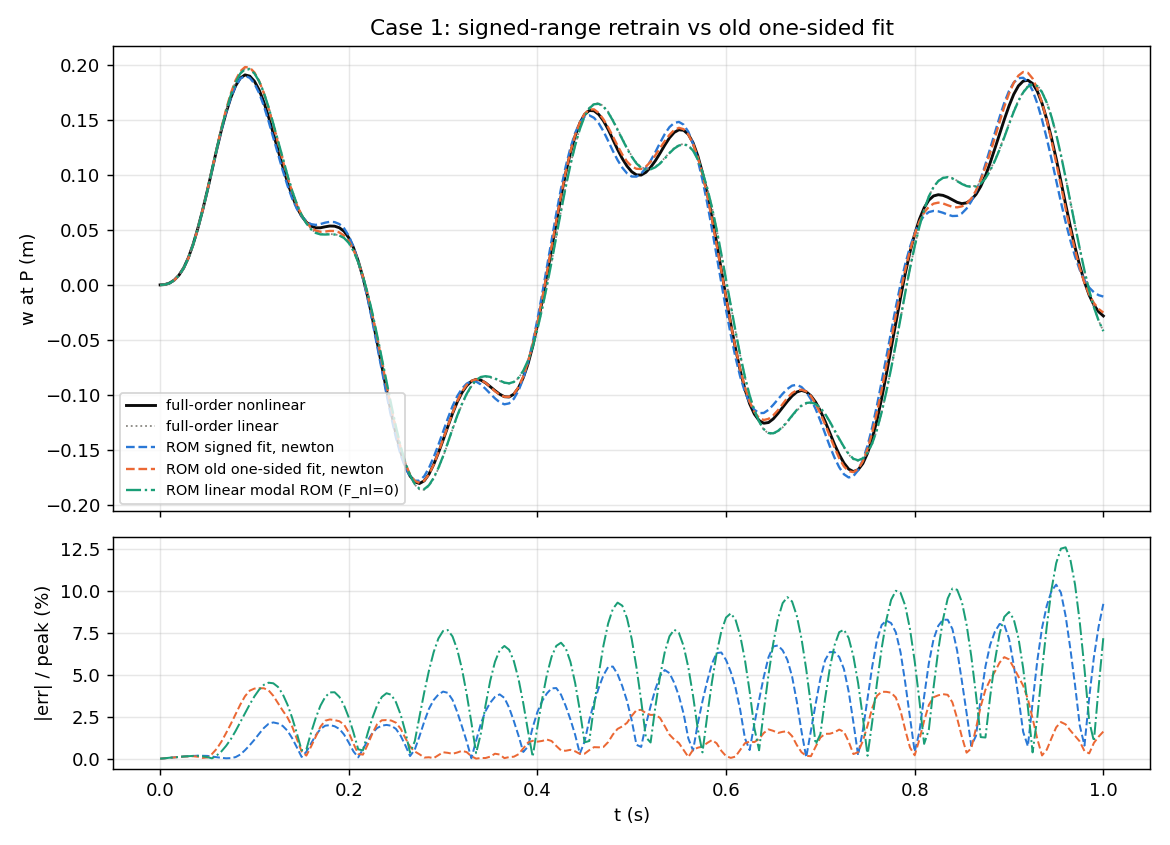
\includegraphics[width=0.8\linewidth]{figures/ch14r/hy_c1_rom.png}
\caption{Case 1: ROM transients against the full-order model. The one-sided earlier fit (trained on the faulty element) agrees only by accident and is not a better model.}\label{fig:vf-hy-c1rom}
\end{figure}

\emph{Backbone.} \Cref{tab:vf-hy-c1back} and \Cref{fig:vf-hy-backbone} show why: the ROM's static solve reproduces the full-order release state to about five digits, yet in free vibration the ROM's frequency shift is $4.7$ to $4.9$ times that of the full-order model. The full-order model retains only about $20\,\%$ of its static hardening in free vibration, because when a cantilever bends its tip moves inward and the inertia of that in-plane motion softens the response; a model trained on static solves contains no in-plane inertia and keeps all of the hardening. This also explains the ranking of \Cref{tab:vf-hy-c1}: the 2.5~Hz forcing is well below the 8.35~Hz mode, so much of the response is quasi-static, where the ROM is right and the linear ROM wrong, while the free-vibration part is where the ROM runs ahead. The report records this as an open defect; the option it recommends is to restore in-plane inertia through the membrane expansion of \rom{}, a change that needs sign-off, and the backbone test is the acceptance check of any fix.

\begin{table}[tbp]
\centering\footnotesize
\caption{Case 1: frequency shift in free vibration released from the static state $q_1$.}\label{tab:vf-hy-c1back}
\begin{tabular}{@{}rrrr@{}}
\toprule
Release $q_1$ & FOM shift & ROM shift & ROM / FOM\\
\midrule
0.05 & $+0.016\,\%$ & $+0.074\,\%$ & 4.7\\
0.10 & $+0.061\,\%$ & $+0.292\,\%$ & 4.8\\
0.15 & $+0.134\,\%$ & $+0.641\,\%$ & 4.8\\
0.20 & $+0.227\,\%$ & $+1.104\,\%$ & 4.9\\
0.25 & $+0.336\,\%$ & $+1.659\,\%$ & 4.9\\
\bottomrule
\end{tabular}
\end{table}

\begin{figure}[tbp]
\centering
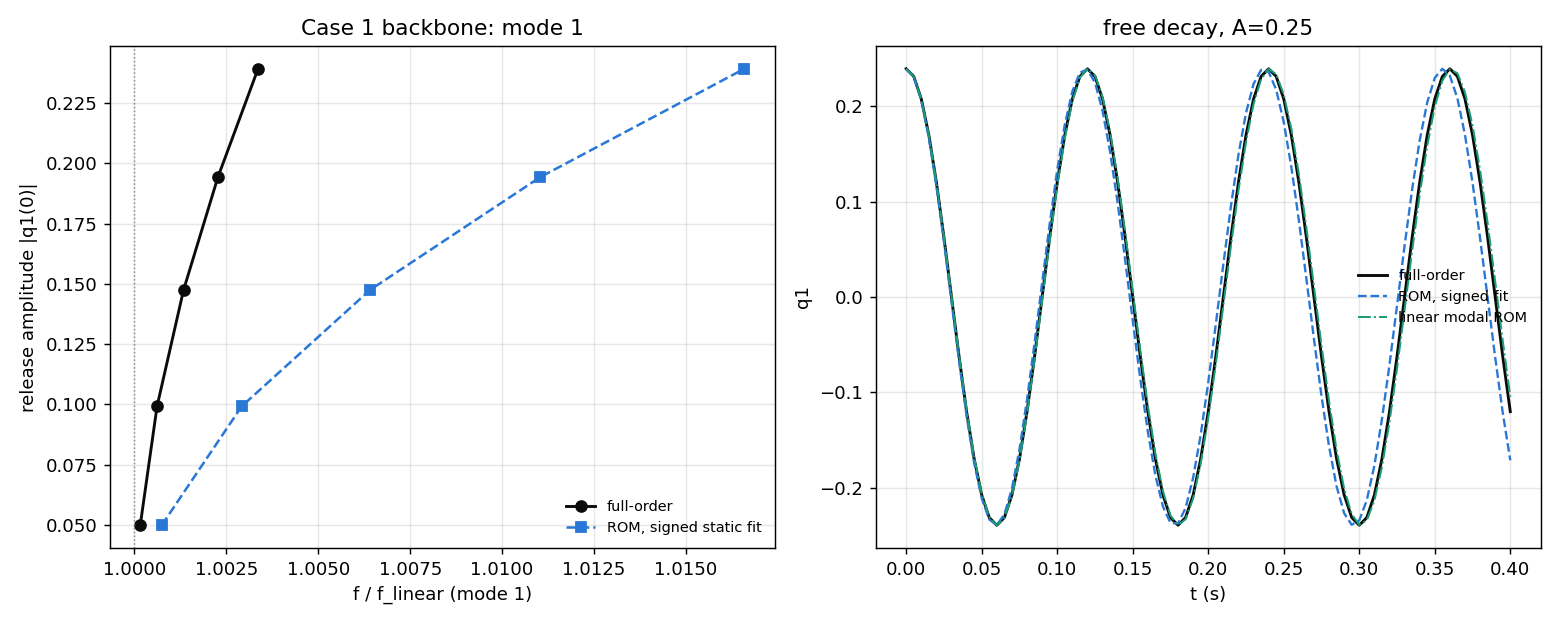
\includegraphics[width=0.8\linewidth]{figures/ch14r/hy_c1_backbone.png}
\caption{Case 1: backbone check. The ROM over-hardens and its phase runs ahead of the full-order model, while the linear ROM tracks it.}\label{fig:vf-hy-backbone}
\end{figure}

\subsection*{Results: case 2, cylindrical panel}

\emph{Static response.} The arc-length full-order solution (30 steps to 31.5~kN) shows a response that softens (tangent stiffness from 446 to about 240~N/mm by 2.5--3.5~kN, crown $w\approx8$--$12$~mm) and then hardens (about 2250~N/mm at 30~kN), matching the publication's softening below about 5000~N (\Cref{fig:vf-hy-c2static}). Ten single-branch Koiter--Newton points between 200~N and 10~kN lie on the curve to $\le10^{-5}$ relative above 600~N ($9\times10^{-4}$ at 200~N, where the interpolated reference is least accurate). The crown displacement is $7.69$~mm at 2.5~kN, $15.69$~mm at 5~kN and $22.46$~mm at 10~kN.

\begin{figure}[tbp]
\centering
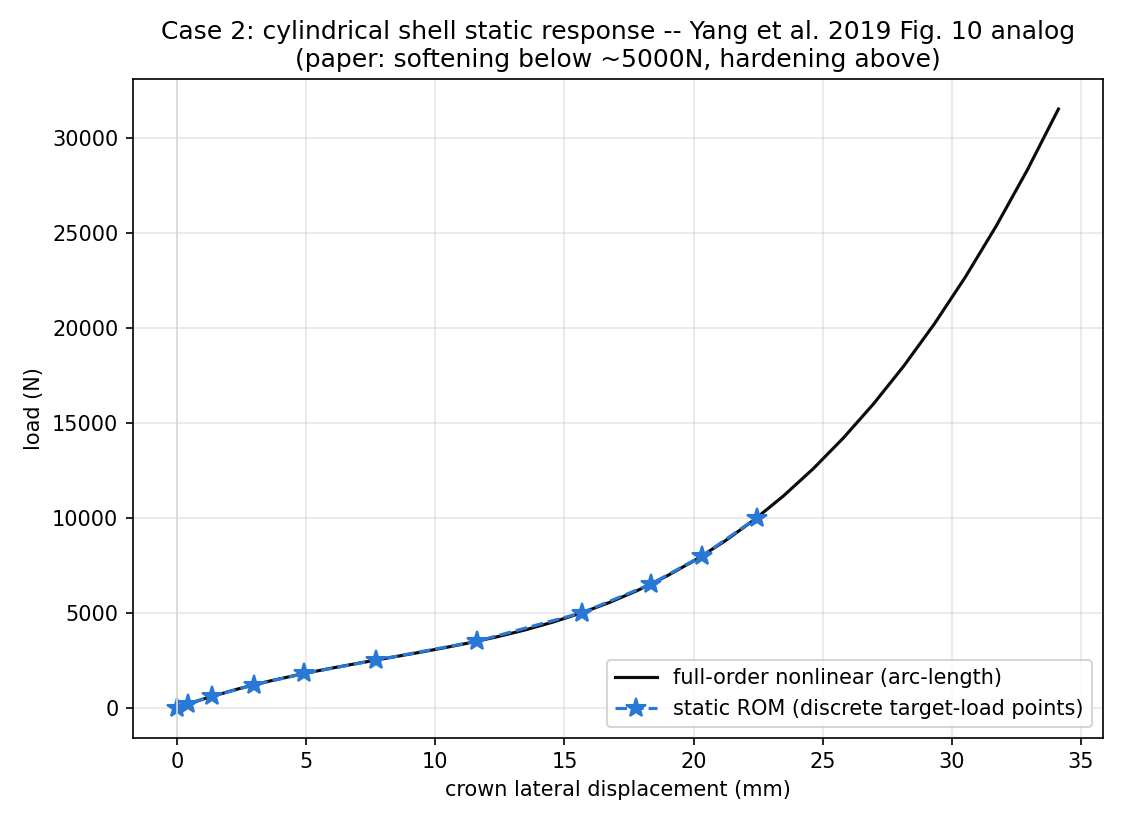
\includegraphics[width=0.7\linewidth]{figures/ch14r/hy_c2_static.png}
\caption{Case 2: static crown response, arc-length full-order solution (line) and Koiter--Newton points (stars).}\label{fig:vf-hy-c2static}
\end{figure}

\emph{Training fit.} Signed per-mode ranges, as fractions of the thickness, are $[-2.2,+2.5]$ for mode~1 and $\pm0.12$, $0.10$, $0.03$, $0.01$, $0.01$ for modes 6, 5, 9, 17, 16. All solves used Koiter--Newton with no fallbacks. \Cref{tab:vf-hy-fit} gives the fit error by mode set.

\begin{table}[tbp]
\centering\footnotesize
\caption{Case 2: training fit by mode set.}\label{tab:vf-hy-fit}
\begin{tabular}{@{}llrr@{}}
\toprule
Set & Modes & Samples & Max relative fit error\\
\midrule
2modes\_top & 1, 6 & 15 & $1.08\,\%$\\
2modes\_alt & 1, 5 & 15 & $0.76\,\%$\\
3modes & 1, 6, 5 & 21 & $0.32\,\%$\\
4modes & 1, 6, 5, 9 & 39 & $0.48\,\%$\\
6modes & 1, 6, 5, 9, 17, 16 & 101 & $1.61\,\%$\\
\bottomrule
\end{tabular}
\end{table}

\emph{Transient.} The full-order crown displacement spans $-12.1$ to $+23.0$~mm against $-16.6$ to $+16.1$~mm for the linear model, so the linear model is off by $70.6\,\%$ of the peak and every ROM here corrects a strongly nonlinear response (\Cref{fig:vf-hy-c2rom}, \Cref{tab:vf-hy-c2}). Two observations follow. Adding modes beyond three does not reduce the ROM error although the truncation floor keeps falling, so the remaining error is fit scatter and not truncation; and retraining over a wider range barely changed the errors, so the $3\,\%$ level is not extrapolation. A diagnostic on the six-mode model recovered the true nonlinear modal force along the transient and compared it with the fit: mode~1's fitted force matches it to $0.65\,\%$ at most ($0.26\,\%$ RMS) over the whole 5000~N transient even though $F_{\rm nl}$ reaches $63\,\%$ of the linear force; correcting mode~1 alone takes the error from $3.13\,\%$ to $1.62\,\%$, mode~6 alone to $2.42\,\%$, mode~5 alone to $2.66\,\%$; adding $q_1^4$ and $q_1^5$ terms does not help ($3.13\,\%$ to $3.13\,\%$), so the polynomial form is not the limit. Fit scatter of $0.3$--$1\,\%$ RMS is amplified about fivefold by the response, an accepted property of the method.

\begin{table}[tbp]
\centering\footnotesize
\caption{Case 2: transient error ($\varepsilon$ of \cref{eq:hy-err}) and the projection floor.}\label{tab:vf-hy-c2}
\begin{tabular}{@{}lrr@{}}
\toprule
Mode set & ROM (\texttt{newton} = \texttt{fixed\_point}) & Projection baseline\\
\midrule
2modes\_top & $6.51\,\%$ & $4.40\,\%$\\
2modes\_alt & $5.35\,\%$ & $5.03\,\%$\\
3modes & $2.83\,\%$ & $1.39\,\%$\\
4modes & $3.68\,\%$ & $0.71\,\%$\\
6modes & $3.13\,\%$ & $0.36\,\%$\\
\bottomrule
\end{tabular}
\end{table}

\begin{figure}[tbp]
\centering
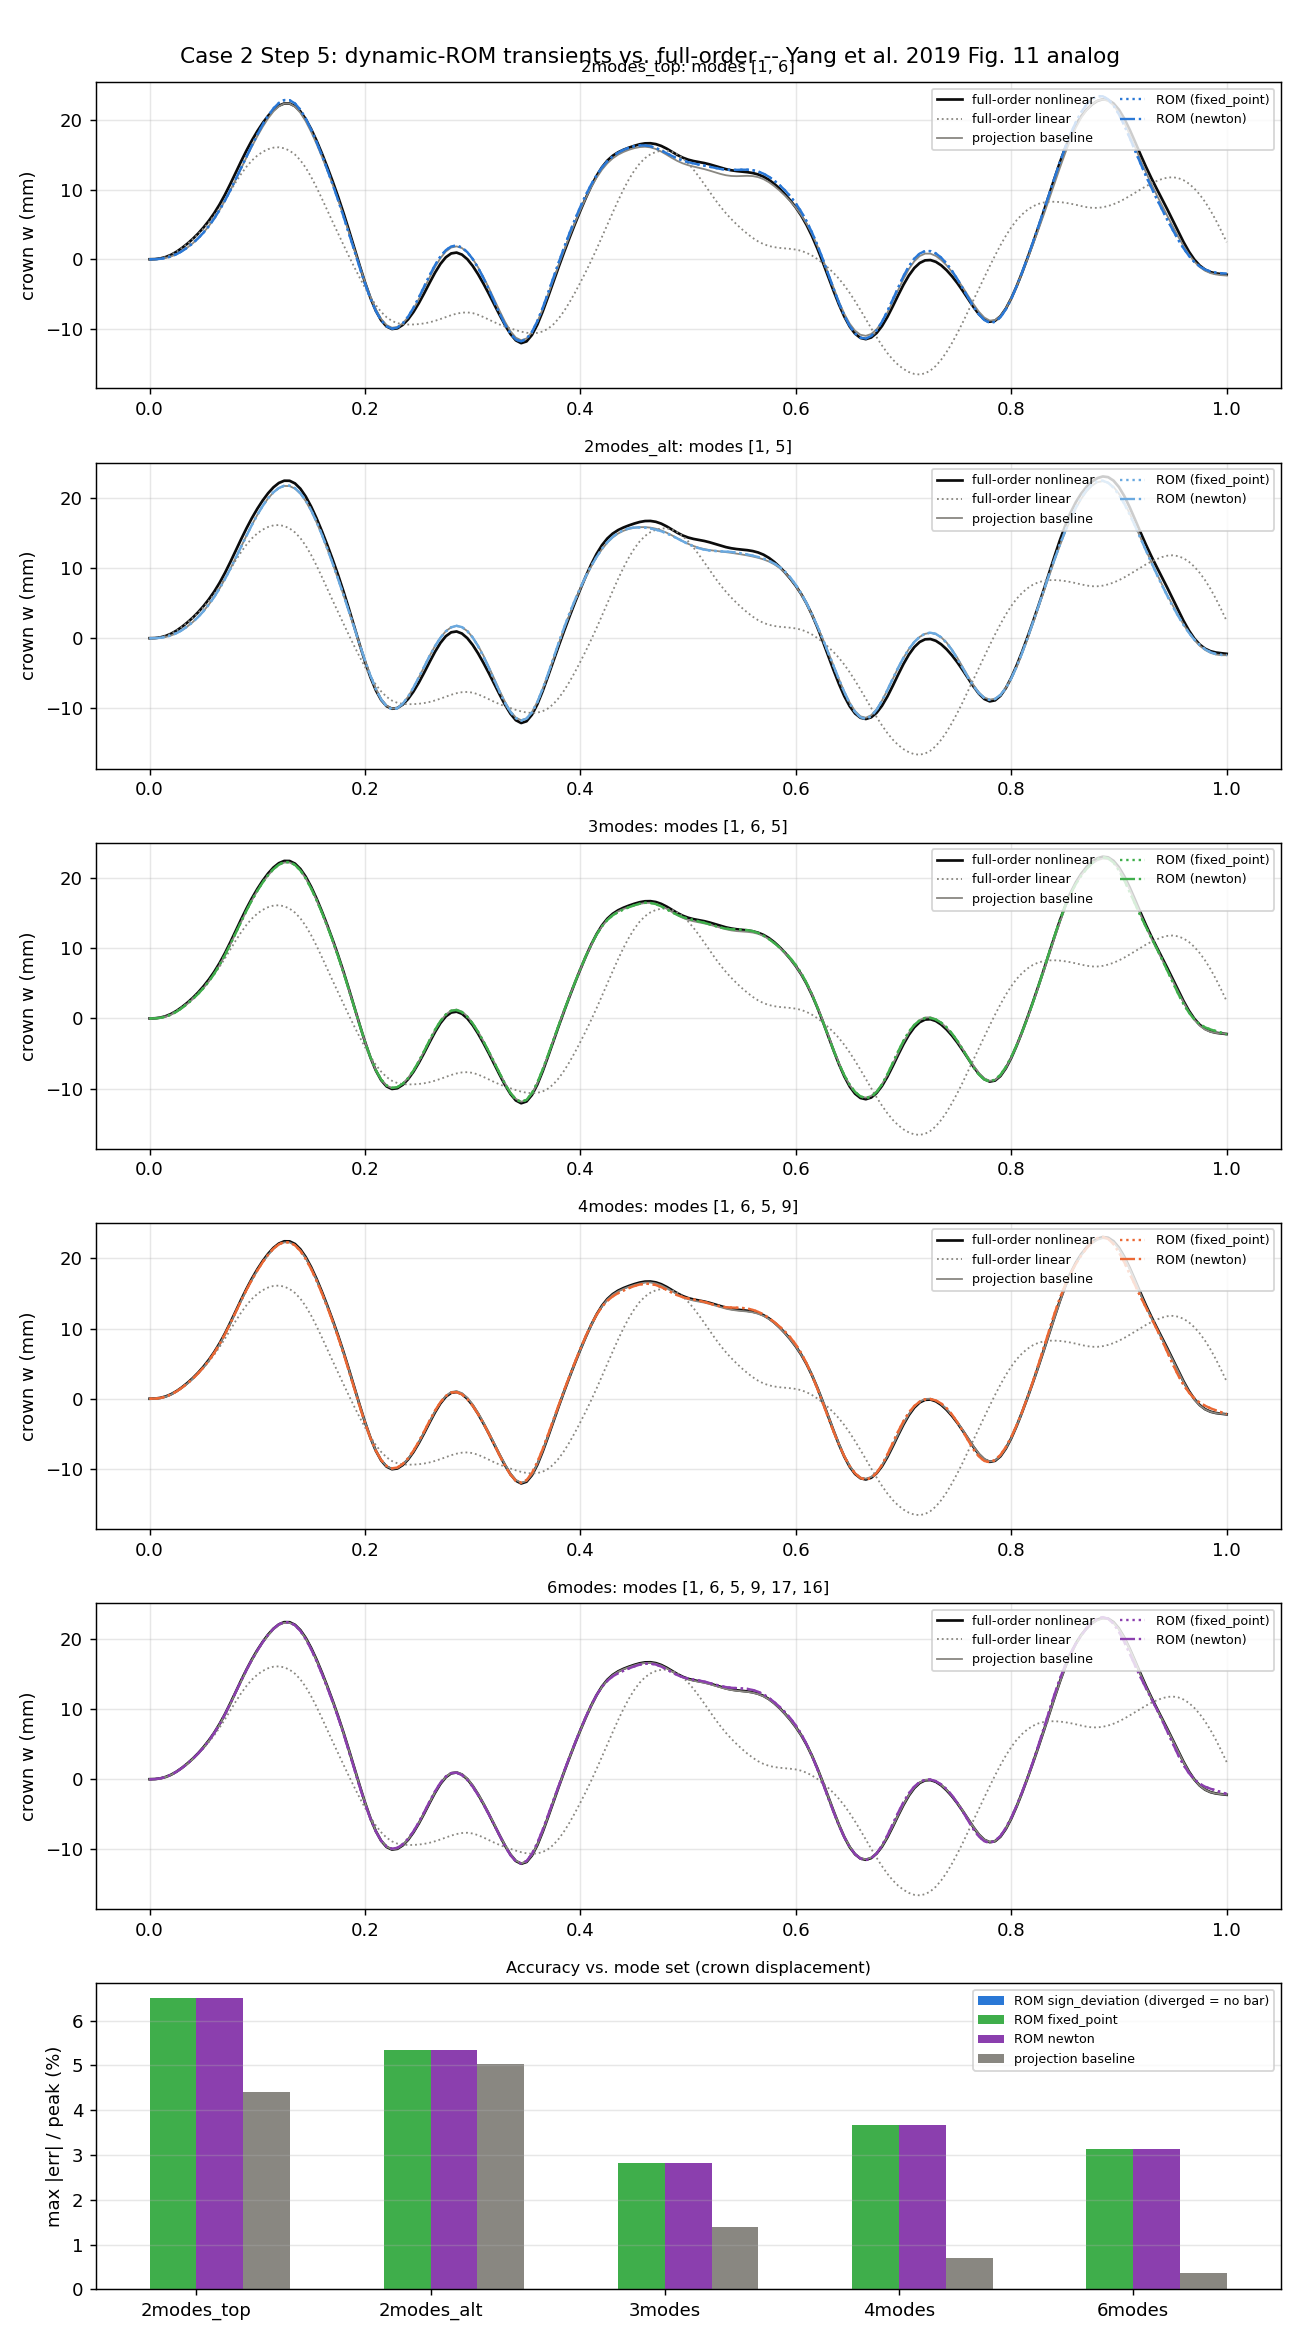
\includegraphics[width=0.75\linewidth]{figures/ch14r/hy_c2_rom.png}
\caption{Case 2: ROM transients for the five mode sets against the full-order crown displacement.}\label{fig:vf-hy-c2rom}
\end{figure}

\emph{Backbone.} Released from ten static states (push-in and pull-out), the orbits cross both sides. \Cref{tab:vf-hy-c2back} gives selected rows: the backbone first softens to $0.962$ and then hardens to $+12\,\%$; the six-mode ROM tracks it to within $0.09\,\%$ at all ten amplitudes and the two-mode ROM to within $0.5\,\%$, even on the two largest orbits, which slightly exceed the training range. The contrast with case~1 is the structure: here the nonlinearity is membrane stretching against fixed edges with no free in-plane motion, so static training captures the dynamics; in case~1 the free edge lets in-plane inertia matter and it does not.

\begin{table}[tbp]
\centering\footnotesize
\caption{Case 2: backbone $f/f_{\rm lin}$ by orbit half-range of $q_1$ (selected rows).}\label{tab:vf-hy-c2back}
\begin{tabular}{@{}rrrr@{}}
\toprule
Half-range $q_1$ & FOM & 6-mode ROM & 2-mode ROM\\
\midrule
2.4 & 0.9859 & 0.9857 & 0.9855\\
5.2 & 0.9624 & 0.9616 & 0.9603\\
6.9 & 0.9706 & 0.9697 & 0.9680\\
9.0 & 1.0209 & 1.0203 & 1.0201\\
10.4 & 1.0775 & 1.0782 & 1.0811\\
11.4 & 1.1197 & 1.1197 & 1.1250\\
\bottomrule
\end{tabular}
\end{table}

\begin{figure}[tbp]
\centering
\includegraphics[width=0.98\linewidth]{figures/ch14_hyrom.pdf}
\caption{Free-vibration check of the hybrid ROM of \citet{yang2019hybrid}: frequency relative to the linear one, full-order model against ROM. (a) Cylindrical panel: the ROM follows the softening and hardening, with a largest frequency error of \cvfHyPanelBack. (b) Plate with a hole: the ROM hardens about \cvfHyPlateRatio{} times too much at the largest amplitude.}\label{fig:vf-hyrom}
\end{figure}

\subsection*{Solver changes the study required}

Six changes to the solver stack were needed to reproduce these results and affect trust in the numbers. (1) \texttt{Shell4MITC}: the two shear rows used the same sign convention, which is wrong for a rotation vector; the defect was invisible on axis-aligned meshes and gave frequencies 3 to 10 times too high on meshes with differently oriented elements (the circular hole), and was found by relabelling the nodes of an element cyclically (the stiffness must be invariant under permutation). (2) \texttt{Shell4Director}: curvature from the moderate to the Green--Lagrange measure. (3) Koiter--Newton: a frozen-tangent chord corrector diverged on a truly nonlinear element. (4) Koiter--Newton: an absolute $10^{-4}$ finite-difference probe was swamped by roundoff at coordinates near 2540~mm and was replaced by a scale-aware probe (default relative step $10^{-2}$). (5) The generic $m=1$ Koiter--Newton driver had a false detection (a trace-based threshold inflated by membrane stiffness) and a corrector that could not move; both were fixed with regression tests. (6) The default integrator of \rom{} changed from \texttt{sign\_deviation} to \texttt{fixed\_point}.

\subsection*{Comparison with the publication}

\begin{table}[tbp]
\centering\footnotesize
\caption{Outcome of the reproduction of \citet{yang2019hybrid}.}\label{tab:vf-hy-cmp}
\begin{tabularx}{\linewidth}{@{}>{\raggedright\arraybackslash}p{3.8cm} >{\raggedright\arraybackslash}X >{\raggedright\arraybackslash}p{2.4cm}@{}}
\toprule
Quantity & This work & Outcome\\
\midrule
Case 1 modes (Table~1) & within $0.3$, $0.9$, $2.8$, $2.9\,\%$; 1224 against 2394 dofs & reproduced\\
Case 1 full-order transient (Fig.~6) & $12.8\,\%$ gap, hardening (publication $\approx20$--$40\,\%$) & partly\\
Case 1 ROM transient & $10.4\,\%$ against $12.6\,\%$ for a linear ROM & partly\\
Case 1 free vibration & ROM over-hardens $4.7$--$4.9\times$ & not reproduced (open defect)\\
Case 2 static response (Fig.~10) & softening then hardening; points on the curve to $\le10^{-5}$ & reproduced\\
Case 2 ROM transient (Fig.~11) & $2.8$--$6.5\,\%$ against a $70.6\,\%$ linear gap & reproduced\\
Case 2 free vibration & within $0.09\,\%$ (6 modes) & reproduced\\
\bottomrule
\end{tabularx}
\end{table}

\subsection*{Departures from the publication's set-up}

The case-1 mesh has 1224 degrees of freedom against the publication's 2394. The training design is optimal Latin hypercube sampling and not the publication's combinatorial grid (its Eqs.~10--14). Case~1's final retraining uses incremental Newton because Koiter--Newton stalls at those amplitudes; case~2 uses Koiter--Newton at discrete target loads and not $m=1$ continuation. The case-2 load is spread over a $3\times3$ patch, and its modes are chosen by load projection, not by hand. The publication's \texttt{sign\_deviation} integrator diverges and is excluded. The remaining limits are the case-1 over-hardening (defect D6), the $12.8\,\%$ against $20$--$40\,\%$ full-order gap, an error floor near $3\,\%$ for three or more modes of case~2, and the lack of an independent reference for the publication's absolute numbers: its figures were compared by reading, not digitising. The main pipeline script of case~1 last ran with the old element and one-sided training, so its outputs are stale and superseded by the standalone scripts; folding the signed training into it and re-running (two hours or more) has not been done. Mode-shape signs depend on the BLAS thread count, so modal quantities are built once in the parent process.

\section{Implicit condensation and expansion}\label{sec:vf-ice}

\subsection*{Concept and purpose}

\citet{hollkamp2008ice} reduce a geometrically nonlinear beam to a few bending modes and identify the nonlinear modal force from static solutions of the full-order model (implicit condensation). Because the linear bending modes of a straight beam have no axial component, the reduced model predicts no in-plane displacement, and the paper recovers it by a second step, the expansion: the in-plane displacement is regressed on the quadratic products of the modal amplitudes. The reduced model is then driven by a random load and compared with the full-order response in time and in the power spectrum, and its in-plane response and stress are recovered. The study tests the identification, the dynamic prediction at two excitation levels, the in-plane expansion and the stress recovery, and the training strategy behind them.

The study uses \anchor{fea_engine.elements.Beam2DCorotational}, the static-fit and polynomial ROM classes of \rom{}, the reduced Newton--Newmark integrator \anchor{rom_engine.integrate_newmark_surrogate} (promoted from the study's prototype) and \anchor{rom_engine.membrane_expansion} for the one-mode expansion. The package gaps found while reproducing (membrane expansion, a multi-mode training strategy, a robust reduced Newton integrator, fibre stress recovery, a band-limited load generator) are recorded in the study's gap analysis, and three of them were closed in the process.

\subsection*{Mathematics as implemented}

With $n$ mass-normalised bending modes, $\boldsymbol\Phi_b^{T}\mathbf M\boldsymbol\Phi_b=\mathbf I$ and $\boldsymbol\Phi_b^{T}\mathbf K\boldsymbol\Phi_b=\boldsymbol\Lambda=\operatorname{diag}(\omega_i^2)$, and $\mathbf u\approx\boldsymbol\Phi_b\mathbf p$, the full-order model $\mathbf M\ddot{\mathbf u}+\mathbf C\dot{\mathbf u}+\mathbf K\mathbf u+\mathbf f_{\rm nl}(\mathbf u)=\mathbf F(t)$ reduces to
\begin{equation}\label{eq:ice-rom}
\ddot p_i+\sum_j\bar c_{ij}\dot p_j+\omega_i^2p_i+\theta_i(\mathbf p)=f_i(t),\qquad\mathbf f=\boldsymbol\Phi_b^{T}\mathbf F,\quad\bar c_{ij}=(\boldsymbol\Phi_b^{T}\mathbf C\boldsymbol\Phi_b)_{ij},
\end{equation}
with the nonlinear modal force in the quadratic-plus-cubic form
\begin{equation}\label{eq:ice-theta}
\theta_i(\mathbf p)=\sum_{j\le k}B_i(j,k)\,p_jp_k+\sum_{j\le k\le l}A_i(j,k,l)\,p_jp_kp_l .
\end{equation}
For a flat structure symmetry removes the quadratic terms and every cubic term with three distinct modes (paper Eq.~7),
\begin{equation}\label{eq:ice-restr}
B_i(j,k)=0,\qquad A_i(j,k,l)=0\ \text{ if $j,k,l$ pairwise distinct},
\end{equation}
which for $n=4$ leaves four self-cubic terms $p_i^3$ and twelve two-mode terms $p_i^2p_j$, 16 coefficients per equation as in the paper; the unrestricted form has 30 (10 quadratic, 20 cubic), and one mode keeps $A_1p_1^3$ only.

\emph{Identification.} Each static sample applies $\mathbf F_s=\mathbf M\boldsymbol\Phi_b\hat{\mathbf f}_s$ and solves the nonlinear static problem for $\mathbf u_s$; projection gives
\begin{equation}\label{eq:ice-id}
\mathbf p_s=\boldsymbol\Phi_b^{T}\mathbf M\mathbf u_s,\qquad\boldsymbol\theta_s=\hat{\mathbf f}_s-\boldsymbol\Lambda\mathbf p_s,
\end{equation}
and the coefficients solve a linear least-squares problem with the monomials of \cref{eq:ice-theta,eq:ice-restr} as the columns of $\boldsymbol\Pi$,
\begin{equation}\label{eq:ice-ls}
\mathbf c=\arg\min_{\mathbf c}\lVert\boldsymbol\Theta-\mathbf c\,\boldsymbol\Pi\rVert_F^2=\boldsymbol\Theta\,\boldsymbol\Pi^{+}.
\end{equation}

\emph{Membrane expansion.} With snapshots $\mathbf W=[\mathbf u_1\cdots\mathbf u_S]$, amplitudes $\mathbf P$ and the quadratic monomials $\mathbf q=[p_1^2,\,p_1p_2,\,\dots,\,p_n^2]^{T}$,
\begin{equation}\label{eq:ice-exp}
\mathbf W-\boldsymbol\Phi_b\mathbf P\approx\mathbf T_m\mathbf Q,\quad\mathbf T_m=[\mathbf W-\boldsymbol\Phi_b\mathbf P]\mathbf Q^{+},\quad\mathbf u(t)=\boldsymbol\Phi_b\mathbf p(t)+\mathbf T_m\mathbf q(t).
\end{equation}
Only the one-mode case is implemented, where $\mathbf q=p_1^2$ and $\mathbf T_m=\sum_s(\mathbf u_s-\boldsymbol\phi_1p_{1,s})\,p_{1,s}^2\big/\sum_sp_{1,s}^4$.

\emph{Reduced Newton--Newmark.} At each step the residual and Jacobian
\begin{equation}\label{eq:ice-newton}
\mathbf R(\mathbf p_{n+1})=\ddot{\mathbf p}_{n+1}+\bar{\mathbf C}\dot{\mathbf p}_{n+1}+\boldsymbol\Lambda\mathbf p_{n+1}+\boldsymbol\theta(\mathbf p_{n+1})-\mathbf f_{n+1},\qquad
\mathbf J=\frac{\mathbf I}{\beta\Delta t^2}+\frac{\gamma\bar{\mathbf C}}{\beta\Delta t}+\boldsymbol\Lambda+\frac{\partial\boldsymbol\theta}{\partial\mathbf p}
\end{equation}
are formed with $\ddot{\mathbf p}_{n+1}$ and $\dot{\mathbf p}_{n+1}$ written through $\mathbf p_{n+1}$ by the Newmark relations, with a line search and an amplitude clamp.

\emph{Fibre stress.} The axial stress at fibre height $y$ of an element is
\begin{equation}\label{eq:ice-stress}
\sigma(\xi,y)=E\left(\frac{\bar e}{L_0}-y\,\kappa(\xi)\right),
\end{equation}
with $\bar e$ the corotational axial extension, $L_0$ the reference length and $\kappa$ the curvature from the corotational end rotations.

\emph{Metric.} All dynamic errors are $\varepsilon=\operatorname{rms}(v_{\rm ROM}-v_{\rm FOM})/\operatorname{rms}(v_{\rm FOM})$ for the transverse displacement at $x=4$~in; a value above 1 means the ROM error exceeds the signal.

\subsection*{Geometry and mesh}

The structure is the aluminium beam of the publication, $18\times1\times0.09$~in, clamped at both ends with immovable ends (\Cref{fig:vf-ice-geom}). The publication models the symmetric half with 36 elements; here the full beam is meshed with 36 \texttt{Beam2DCorotational} elements ($\Delta x=0.5$ in) and the symmetric modes are picked by a mirror-symmetry score above $0.9$. \Cref{tab:vf-ice-setup} lists what is shared with the publication and what was chosen.

\begin{figure}[tbp]
\centering
\includegraphics[width=0.98\linewidth]{figures/ch14_geom_ice.pdf}
\caption{Flat beam of the ICE study, drawn from the dimensions of the report: 36 elements, clamped ends, the observation point at $x=4$ in and the spatially uniform random load.}\label{fig:vf-ice-geom}
\end{figure}

\begin{table}[tbp]
\centering\footnotesize
\caption{Set-up of the ICE study.}\label{tab:vf-ice-setup}
\begin{tabularx}{\linewidth}{@{}>{\raggedright\arraybackslash}p{2.8cm} >{\raggedright\arraybackslash}X >{\raggedright\arraybackslash}X@{}}
\toprule
Item & Publication & This work\\
\midrule
Geometry, material & $18\times1\times0.09$ in; $E=10.6\times10^6$ psi, $G=4.0\times10^6$ psi, $\rho=2.588\times10^{-4}$ lb s$^2$/in$^4$ & same ($\nu=0.325$)\\
Mesh & symmetric half, 36 elements & full beam, 36 elements\\
Retained modes & 4 symmetric bending modes & 1 and 4\\
Excitation & uniform, Gaussian, band-limited 0--1500 Hz, 0.9216 and 0.0072 lb/in RMS & same; spectral synthesis, seed 42\\
Damping & not recorded here & Rayleigh, mass-proportional, $\zeta_1=0.02$, in FOM and ROM\\
Time integration & not recorded here & 20\,000 steps, $\Delta t=5\times10^{-5}$ s, $T=1$ s; implicit Newmark (FOM about 240 s per run)\\
Training, 4 modes & not stated & 150 static solves, target $\pm3\times0.09$ in per mode (Latin hypercube), 12 held out\\
Training, 1 mode & not stated & 60 samples at $\pm150$, 15 kept for testing (set A); 20 samples at $\pm3$ (set B)\\
Neural surrogate & none & multilayer perceptron (MLP), 4000 epochs, 150 static samples\\
Trajectory states & none & 80 states from short FOM transients (6\,002 visited) added to the 150\\
\bottomrule
\end{tabularx}
\end{table}

\subsection*{Results: modes and static identification}

The four symmetric bending frequencies are within $0.21\,\%$ of the publication's Table~2 (\Cref{tab:vf-ice-modes}, \Cref{fig:vf-ice-modes}). The static fit of the nonlinear modal force reaches unseen $R^2$ of $0.9998$ for one mode, $0.99998$ for four modes (unrestricted polynomial, 30 terms) and $0.99935$ for the neural surrogate. The static fits are as good as the method requires; they do not predict the dynamic outcome below.

\begin{table}[tbp]
\centering\footnotesize
\caption{Linear symmetric bending frequencies.}\label{tab:vf-ice-modes}
\begin{tabular}{@{}rrrr@{}}
\toprule
Mode & This work (Hz) & Publication (Hz) & Difference\\
\midrule
1 & 57.8 & 57.8 & $0.00\,\%$\\
2 & 312.3 & 312.1 & $0.06\,\%$\\
3 & 771.1 & 770.3 & $0.10\,\%$\\
4 & 1434.1 & 1431.2 & $0.20\,\%$\\
\bottomrule
\end{tabular}
\end{table}

\begin{figure}[tbp]
\centering
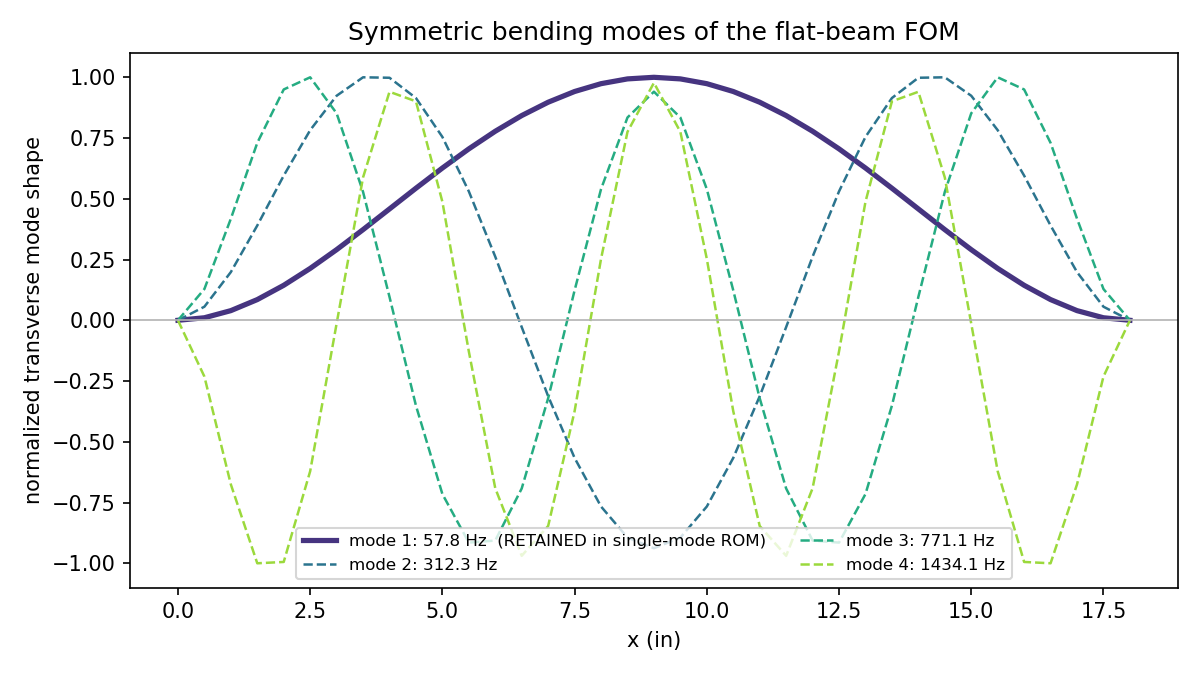
\includegraphics[width=0.85\linewidth]{figures/ch14r/ice_modes.png}
\caption{The four retained symmetric bending modes. The one-mode ROM keeps only the first.}\label{fig:vf-ice-modes}
\end{figure}

\subsection*{Results: one-mode dynamics}

\Cref{fig:vf-ice} shows the displacement at $x=4$~in and its power spectral density for the two levels. At the low level the ROM follows the waveform and the first-mode peak and misses the peaks near 312 and 1400~Hz (modes not retained); at the high level it follows the full-order response for about 0.1~s and then loses phase. The errors are $19.5\,\%$ (low) and $136\,\%$ (high) for the first set of settings; the peak $|q_{\rm nl}|$ is $1.1\times10^{-4}$ at the low level and $5.8\times10^{-3}$ at the high level against a training peak of $7.4\times10^{-3}$.

\begin{figure}[tbp]
\centering
\includegraphics[width=0.9\linewidth]{figures/ch14_ice.pdf}
\caption{One-mode ICE ROM against the full-order model for the flat beam of \citet{hollkamp2008ice}: displacement at $x=4$~in over the first $0.2$~s and its power spectral density, at the low level (RMS error \cvfIceLowRms) and the high level (RMS error \cvfIceHighRms).}\label{fig:vf-ice}
\end{figure}

\emph{Why two one-mode runs differ at the high level.} Two scripts ran the one-mode case with different ROMs against the same full-order response (the saved histories match exactly, same load seed). \Cref{tab:vf-ice-two} lists them; a study crossing the two training sets with both clamp multipliers (6 and 20 times the training peak) and three training seeds follows in \Cref{tab:vf-ice-seeds}.

\begin{table}[tbp]
\centering\footnotesize
\caption{The two one-mode ROMs.}\label{tab:vf-ice-two}
\begin{tabular}{@{}lllllrr@{}}
\toprule
Script & Training & Peak training $|q_{\rm nl}|$ & Cubic coefficient & Clamp & $\varepsilon$ low & $\varepsilon$ high\\
\midrule
\texttt{reproduce\_flat\_beam.py} & 60 samples, $\pm150$ (A) & $7.4\times10^{-3}$ & $5.45\times10^{10}$ & 6$\times$ & 0.1946 & 1.362\\
\texttt{reproduce\_fig1.py} & 20 samples, $\pm3$ (B) & $1.5\times10^{-3}$ & $6.61\times10^{10}$ & 20$\times$ & 0.1944 & 1.145\\
\bottomrule
\end{tabular}
\end{table}

\begin{table}[tbp]
\centering\footnotesize
\caption{One-mode study over training set, clamp and training seed.}\label{tab:vf-ice-seeds}
\begin{tabular}{@{}lrrl@{}}
\toprule
Training set & $\varepsilon$ low (all seeds, both clamps) & $\varepsilon$ high, seeds 0 / 1 / 2 & Range\\
\midrule
A (60 samples, $\pm150$) & 0.1946 & 1.362 / 1.261 / 1.258 & 1.26--1.36\\
B (20 samples, $\pm3$) & 0.1944 & 1.145 / 1.118 / 1.147 & 1.12--1.15\\
\bottomrule
\end{tabular}
\end{table}

The clamp has no effect (the ROM never reaches either bound, so 6 and 20 times give identical errors to every digit). The cubic coefficient differs by about $21\,\%$ between the sets, and at the high level the two ROMs reach similar peaks (about $5$--$6\times10^{-3}$) but follow different trajectories; why the wider-amplitude set fits softer was not tested, and a non-cubic component of the true force at larger amplitude is one possibility. Seed sensitivity is modest (about $0.1$ for set A, $0.03$ for set B, none at the low level; only the training seed was varied, not the load seed). The conclusion is unchanged: every one-mode ROM exceeds 1 at the high level, and the figure to quote is $1.12$--$1.36$.

\subsection*{Results: in-plane displacement}

\Cref{fig:vf-ice-inplane} compares the in-plane spectrum at $x=4$~in of the full-order model with the one-mode ICE model and membrane expansion. At the high level the spectra agree below about 400~Hz and the expanded response then falls away by many orders of magnitude; at the low level the model lacks the spectral peaks of the full-order response. With one mode \cref{eq:ice-exp} gives $u(t)=T_mp_1(t)^2$ and $p_1^2\ge0$, so the predicted in-plane motion keeps one sign and follows a slow envelope while the full-order motion oscillates about zero. This is a limit of the one-mode expansion, independent of the quality of the fit. Peak in-plane values at the high level are $3.89\times10^{-3}$~in (full order) and $2.34\times10^{-3}$~in (ROM).

\begin{figure}[tbp]
\centering
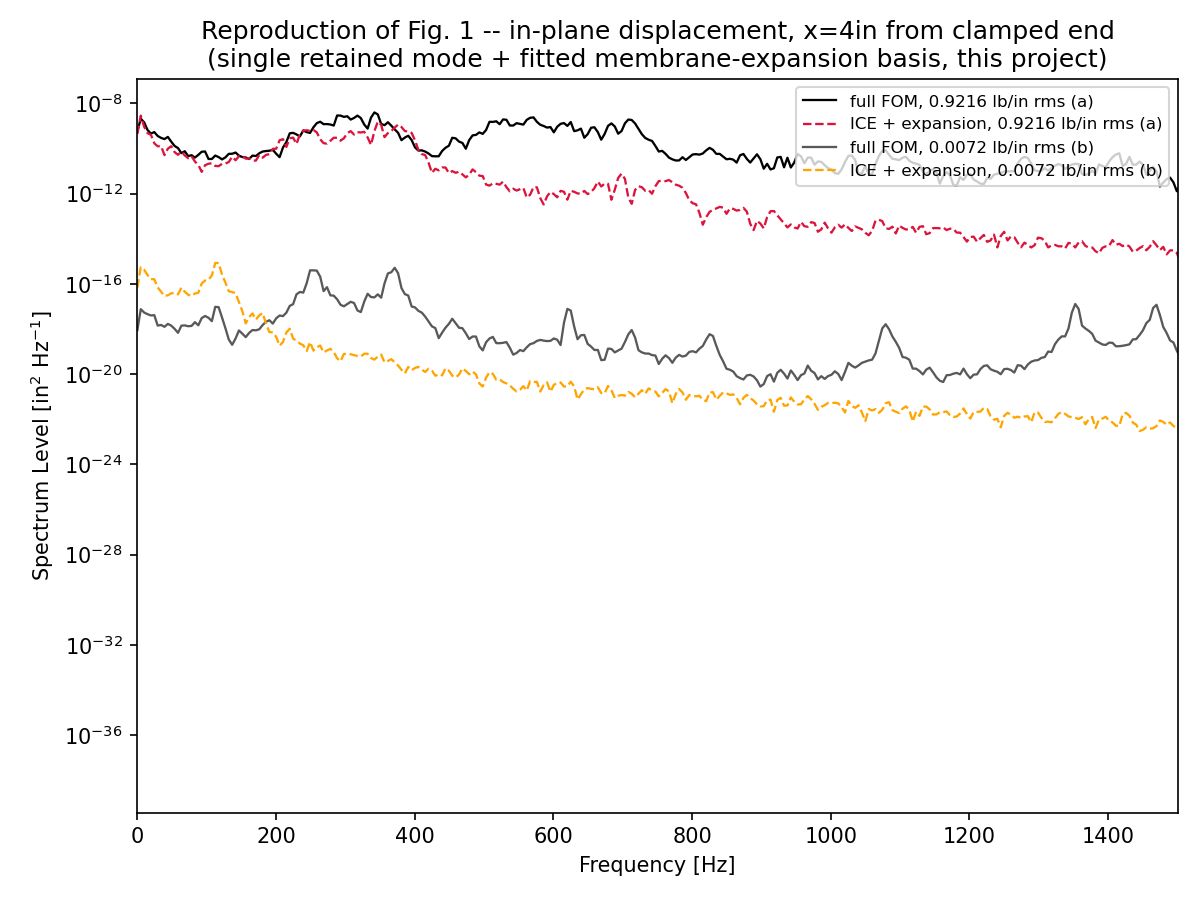
\includegraphics[width=0.8\linewidth]{figures/ch14r/ice_inplane.png}
\caption{In-plane displacement spectrum at $x=4$ in. Solid: full-order model; dashed: single-mode ICE with membrane expansion. Upper pair: high level; lower pair: low level.}\label{fig:vf-ice-inplane}
\end{figure}

\subsection*{Results: four modes and the training distribution}

\Cref{tab:vf-ice-four} and \Cref{fig:vf-ice-variants} give the four-mode variants. The restricted form of \cref{eq:ice-restr} is worse than the unrestricted one in this comparison; adding states from short full-order transients (trajectory-piloted samples) improves both levels, by a factor of about $3$ at the low level and $1.5$ at the high level, and does not bring the high level below 1. A neural surrogate with static $R^2=0.99935$ diverges: the reduced response grows to a peak of about 78~in in the first 0.2~s while the full-order response peaks at $0.0045$~in (low) and $0.24$~in (high) (\Cref{fig:vf-ice-neural}).

\begin{table}[tbp]
\centering\footnotesize
\caption{Four-mode dynamics by variant.}\label{tab:vf-ice-four}
\begin{tabular}{@{}lrr@{}}
\toprule
Variant & $\varepsilon$ low & $\varepsilon$ high\\
\midrule
Polynomial, restricted form, static samples only & 0.336 & 7.93\\
Polynomial, unrestricted, static samples only & 0.0645 & 2.00\\
Polynomial, unrestricted, static + trajectory-piloted samples & 0.0219 & 1.35\\
Neural surrogate (MLP), static samples only & $3.3\times10^{4}$ & 538\\
\bottomrule
\end{tabular}
\end{table}

\begin{figure}[tbp]
\centering
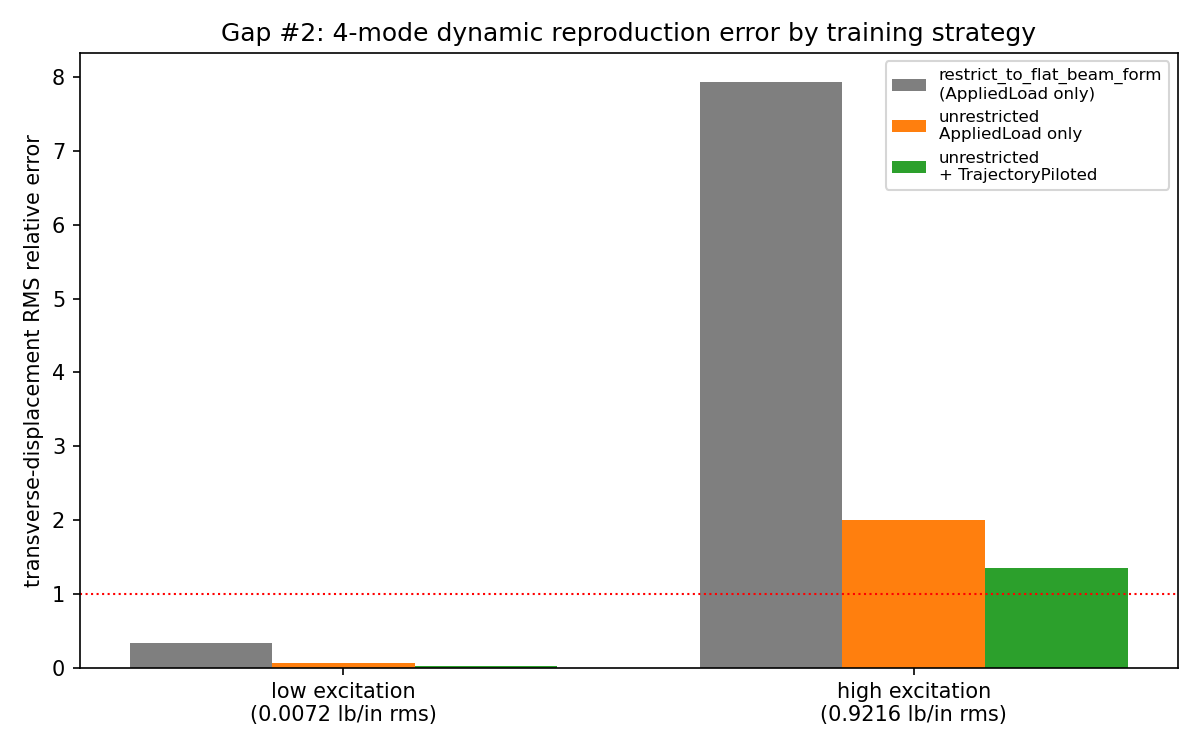
\includegraphics[width=0.7\linewidth]{figures/ch14r/ice_variants.png}
\caption{Four-mode RMS error by training strategy; the dotted line at 1 marks an error equal to the full-order signal.}\label{fig:vf-ice-variants}
\end{figure}

\begin{figure}[tbp]
\centering
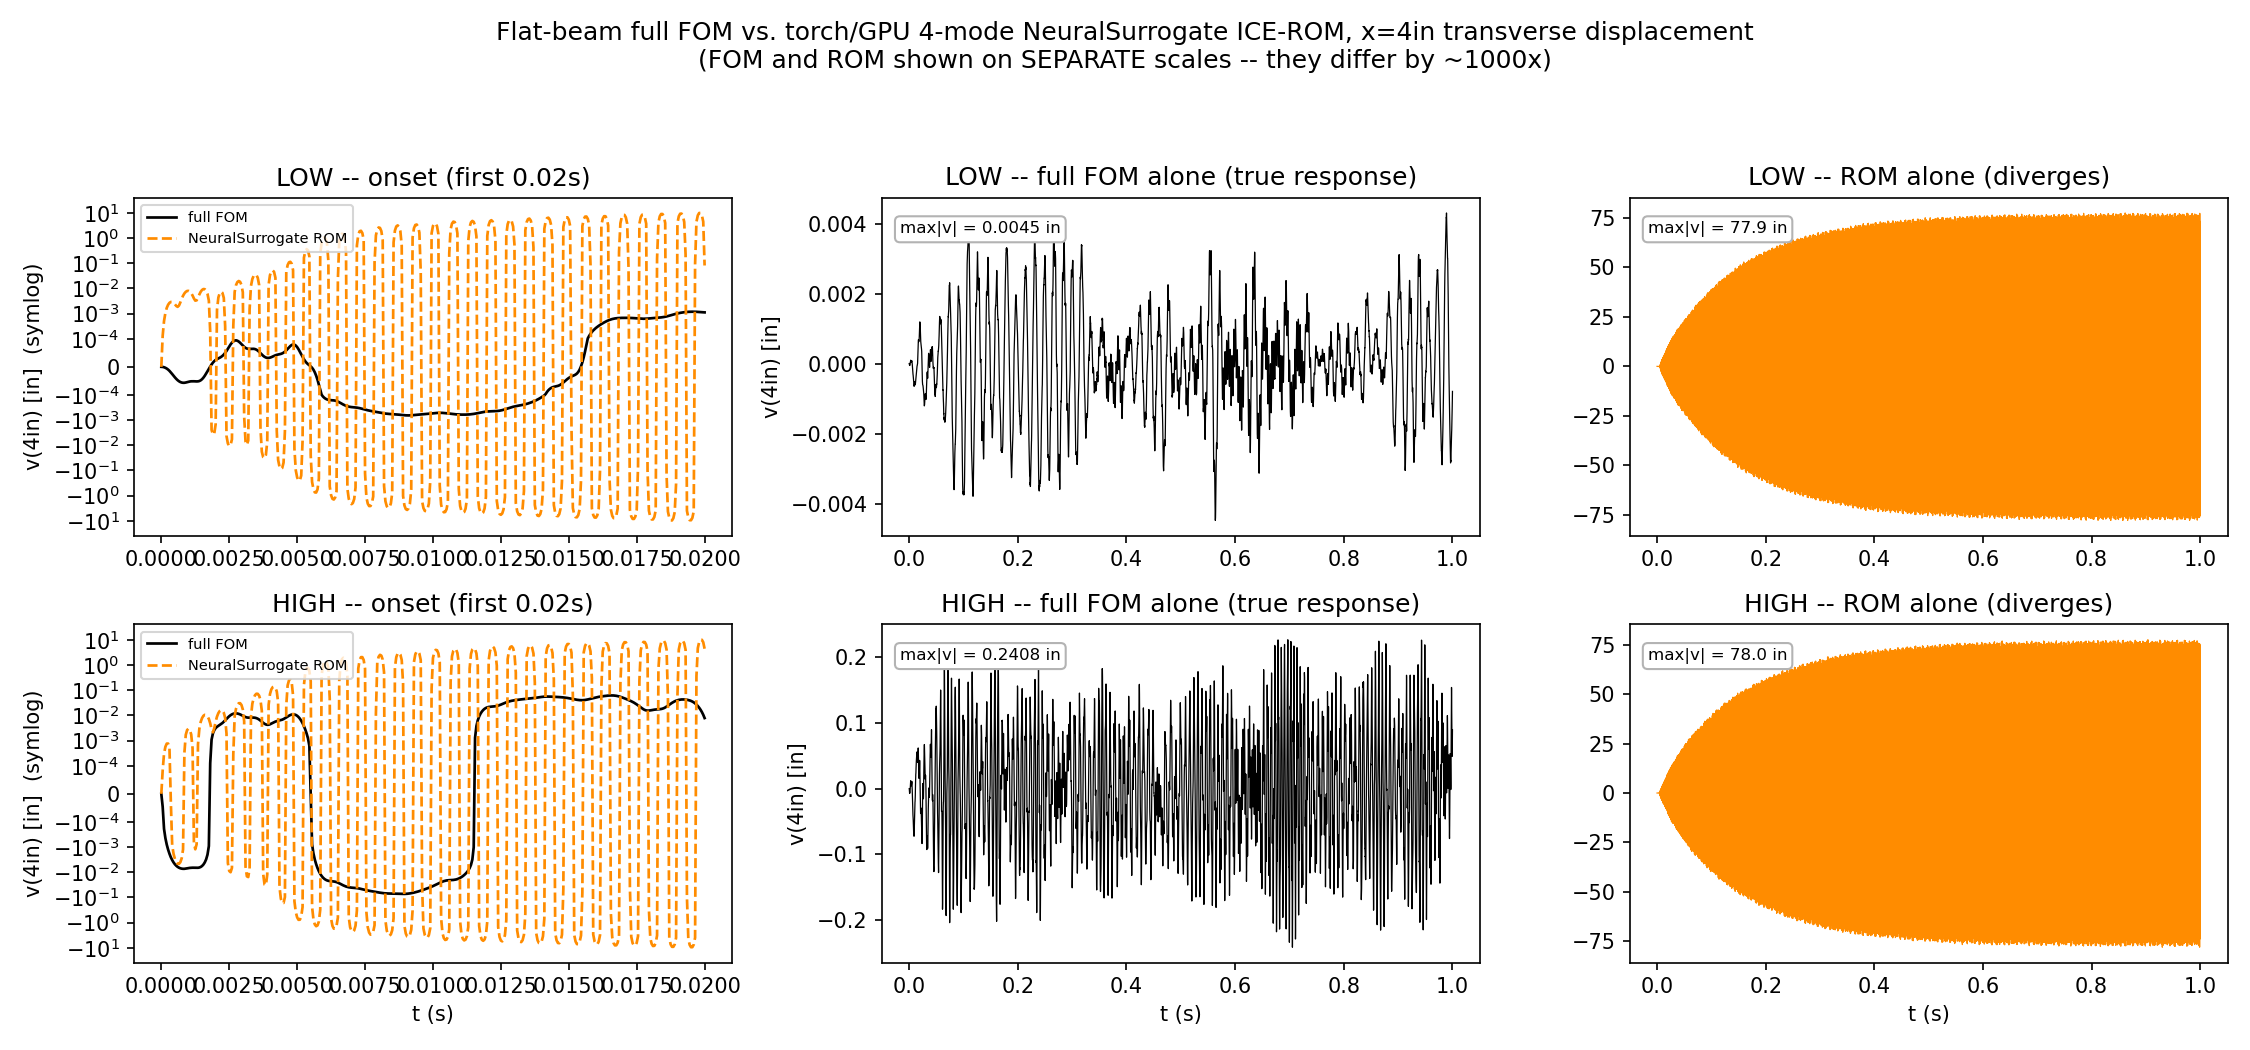
\includegraphics[width=0.8\linewidth]{figures/ch14r/ice_neural.png}
\caption{Four-mode neural ICE ROM against the full-order model, on separate scales about 1000 times apart.}\label{fig:vf-ice-neural}
\end{figure}

Two regressors of different type, with static $R^2$ above $0.999$, fail in the same way, which points at the training distribution and not at the regression: the static sampling strategy draws each mode's target displacement independently, whereas a random response visits coupled, sign-varying combinations. Adding states from full-order transients reduces the four-mode error by a factor of $1.5$ to $3$, consistent with a coverage problem. Whether broader or iterated training (refit, re-simulate, add points where ROM and full-order response disagree) brings the high level below 1 was not run.

\subsection*{Results: integrator and stress recovery}

The reduced Newton--Newmark routine of the package, \texttt{integrate\_newmark\_surrogate} with \texttt{correction='newton'}, matches the study's prototype integrator exactly: over 0.1~s on the four-mode case the maximum absolute difference in $q_{\rm nl}$ is exactly 0 (\Cref{fig:vf-ice-integ}). The built-in lag-correction schemes diverged to NaN on the polynomial model, which is why the prototype was written. Stress recovery by \cref{eq:ice-stress} was evaluated for one training snapshot with 0.31~in peak transverse amplitude (\Cref{fig:vf-ice-stress}): along element~7 the mid-plane (membrane) stress is $22.4$~ksi, the top fibre about $26$--$27$~ksi and the bottom fibre about $18$--$19$~ksi, so the membrane part dominates, as the publication relies on. This was not checked against full-order element stresses and so does not validate the publication's stress-PSD figures.

\begin{figure}[tbp]
\centering
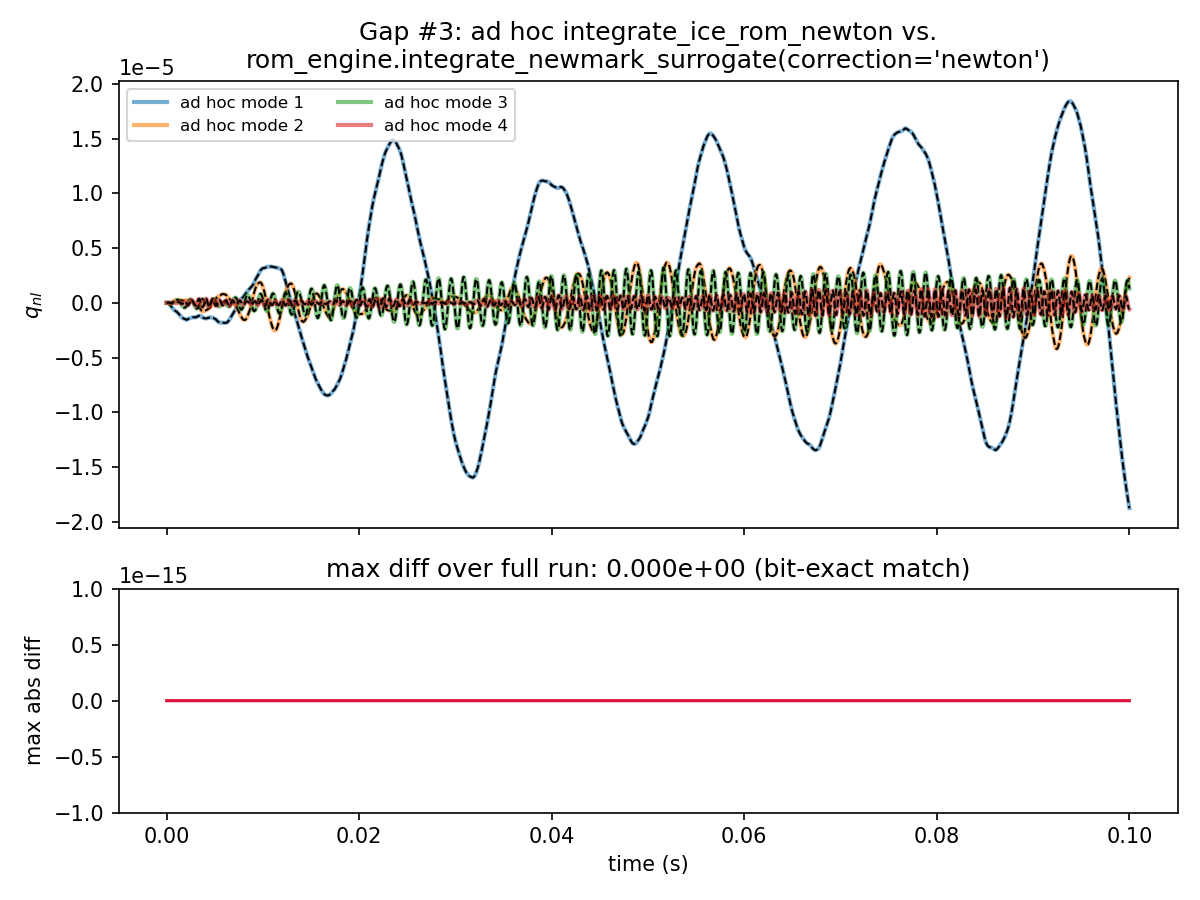
\includegraphics[width=0.8\linewidth]{figures/ch14r/ice_integrator.png}
\caption{Modal trajectories from the prototype integrator (colour) and the package routine (black dashed), with the difference below.}\label{fig:vf-ice-integ}
\end{figure}

\begin{figure}[tbp]
\centering
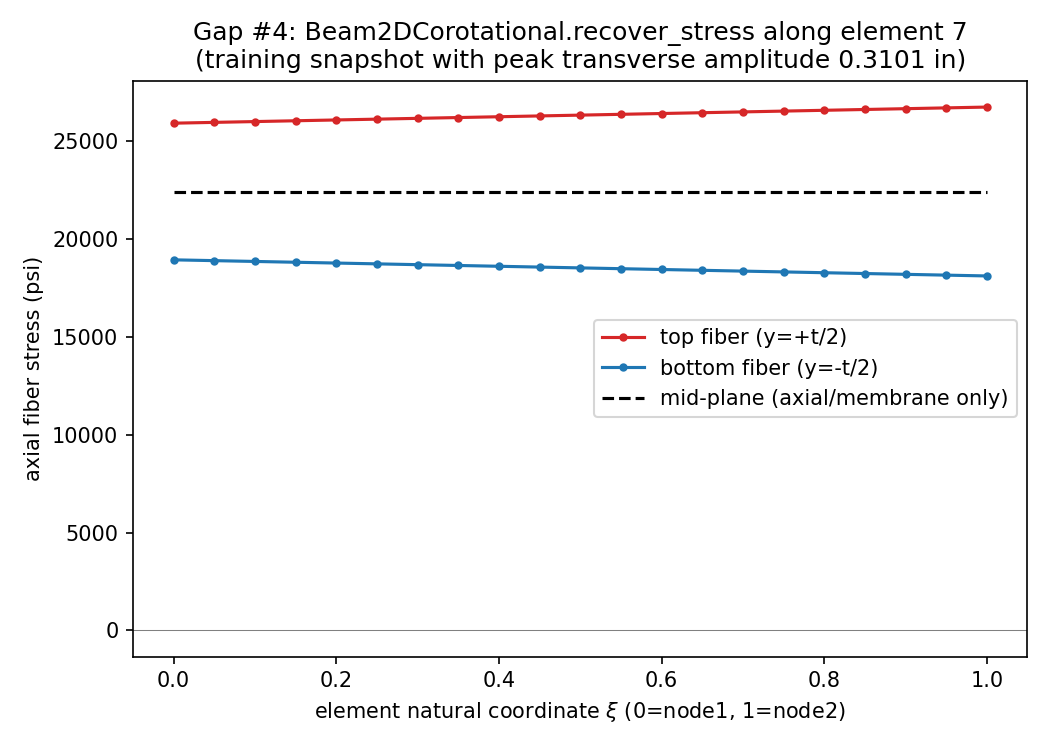
\includegraphics[width=0.7\linewidth]{figures/ch14r/ice_stress.png}
\caption{Axial stress along element 7 for a training snapshot with 0.31 in peak transverse amplitude.}\label{fig:vf-ice-stress}
\end{figure}

\subsection*{Comparison with the publication}

\begin{table}[tbp]
\centering\footnotesize
\caption{Claims of \citet{hollkamp2008ice} and the outcome of the reproduction.}\label{tab:vf-ice-cmp}
\begin{tabularx}{\linewidth}{@{}>{\raggedright\arraybackslash}p{4.0cm} >{\raggedright\arraybackslash}X >{\raggedright\arraybackslash}p{2.3cm}@{}}
\toprule
Claim & This work & Outcome\\
\midrule
Linear modes (Table~2) & $57.8/312.3/771.1/1434.1$ against $57.8/312.1/770.3/1431.2$ Hz & reproduced\\
Nonlinear force identified from static solutions & unseen $R^2$ 0.9998 (1 mode), 0.99935--0.99998 (4 modes) & reproduced\\
Accurate random response, low level & $19.5\,\%$ (1 mode); $2.2$--$33.6\,\%$ (4 modes, by variant) & partly\\
Accurate random response, high level & $112$--$136\,\%$ (1 mode); $135$--$793\,\%$ (4 modes) & not reproduced\\
Membrane expansion recovers in-plane displacement (Fig.~1) & agrees below about 400 Hz at the high level only; one-sign signal & not reproduced\\
Stress recovery from the expanded field & implemented, one snapshot, no full-order comparison & not validated\\
\bottomrule
\end{tabularx}
\end{table}

\subsection*{How the comparison was judged}

The comparison is of the ROM against the full-order model, not an overlay of the publication's plots, so ``not reproduced'' is judged from error levels, and the publication's own dynamic accuracy figures were not extracted from the PDF. Several settings that the publication does not give (damping, time step, training sizes, the load realisation) were chosen here and can change the numbers. The one-mode case has a three-seed study on the training seed only; the four-mode variants are one training run each, and differences between them below a factor of about 2 should not be read as significant. The membrane expansion is implemented for one mode only; whether a four-mode $\mathbf T_m$ (ten quadratic terms in \cref{eq:ice-exp}) repairs the in-plane spectrum was not tried. Stress recovery has no full-order comparison. Finally, why a wider training amplitude gives a softer cubic coefficient was measured but not explained.

\Cref{tab:vf-ice-gaps} records what the study predicted from the package gap analysis and what happened.

\begin{table}[tbp]
\centering\footnotesize
\caption{Package gaps found before the study and their outcome.}\label{tab:vf-ice-gaps}
\begin{tabularx}{\linewidth}{@{}>{\raggedright\arraybackslash}p{4.2cm} >{\raggedright\arraybackslash}X@{}}
\toprule
Gap & Outcome\\
\midrule
Membrane basis and expansion missing & implemented for one mode; result above\\
Multi-mode training strategy missing & confirmed by experiment; the trajectory-piloted prototype helps by a factor $1.5$--$3$, not enough at the high level\\
Robust reduced Newton integrator missing & promoted to the package; bit-exact against the prototype\\
Fibre stress recovery missing & \texttt{Beam2DCorotational.recover\_stress} plotted for one snapshot; not validated\\
Band-limited forcing generator missing & ad hoc version used in all runs\\
\bottomrule
\end{tabularx}
\end{table}

\section{Matrix-free modal identification of a fluid-loaded plate}\label{sec:vf-fsi}

\subsection*{Concept and purpose}

\citet{liu2026fsi} identify the natural frequencies, damping ratios and mode shapes of a fluid-loaded structure from scalar frequency-response samples at one reference point, without access to the mass, damping or stiffness matrices and without knowing the force. A Loewner pencil built from two interleaved sets of sampled frequencies turns the identification into a small generalised eigenproblem, and a screening step that compares many such models separates physical modes from spurious ones. The study tests the method on a steel plate in air and in water: the identification error against a reference, the effect of mesh, boundary condition, excitation, sample density, band, sensor position and noise, and the quality of the recovered mode shapes. It is the study that uses \rom{}'s Loewner and screening modules (\anchor{rom_engine.loewner}, \anchor{rom_engine.screening}) on a model from \fea{}.

\subsection*{Mathematics as implemented}

A linear structure, possibly fluid-loaded, responds to a harmonic force $\mathbf Fe^{i\omega t}$ with
\begin{equation}\label{eq:fsi-frf}
\mathbf x(\omega)=\mathbf T(\omega)^{-1}\mathbf F,\qquad\mathbf T(\omega)=\mathbf K+i\omega\mathbf C-\omega^2\mathbf M\quad(-\,\omega^2\mathbf M_f(\omega)\ \text{if fluid-loaded}).
\end{equation}
The modal parameters are the complex roots $\omega_k^\ast$ of $\det\mathbf T(\omega)=0$, reported as $f_k=\operatorname{Re}\omega_k^\ast/2\pi$ and $\eta_k=\operatorname{Im}\omega_k^\ast/\operatorname{Re}\omega_k^\ast$.

\emph{Loewner pencil.} Two disjoint interpolation sets $\{\omega_a\}_{a=1}^n$ and $\{\omega_b\}_{b=1}^n$ give samples $x_a=x(\omega_a)$, $x_b=x(\omega_b)$ and the $n\times n$ matrices
\begin{equation}\label{eq:fsi-loewner}
\tilde A_{ab}=\frac{\omega_a^{2}x_a-\omega_b^{2}x_b}{\omega_a^{2}-\omega_b^{2}},\qquad
\tilde E_{ab}=\frac{x_a-x_b}{\omega_a^{2}-\omega_b^{2}},\qquad
\tilde A\tilde\Phi=\tilde E\tilde\Phi\tilde\Lambda,\quad\lambda_i=\omega_i^2 .
\end{equation}
For a frequency-independent system each response is a rational function of $\lambda=\omega^2$, $x(\lambda)=N(\lambda)/D(\lambda)$ with $\deg D$ equal to the number of modes; the divided differences are its Loewner matrices and the generalised eigenvalues are its poles, the complex squared natural frequencies with damping included. With exact data and $n$ at least the number of modes in the data, the poles are recovered to round-off; a larger $n$ produces extra, non-physical eigenpairs that the screening removes.

\emph{Mode shapes.} Responses at $m$ measurement points sampled at the same $\{\omega_b\}$, $\mathbf X_\beta\in\mathbb C^{m\times n}$, give $\boldsymbol\Phi=\mathbf X_\beta\tilde\Phi$, compared with reference shapes by the modal assurance criterion
\begin{equation}\label{eq:fsi-mac}
\mathrm{MAC}(\boldsymbol\phi_a,\boldsymbol\phi_b)=\frac{|\boldsymbol\phi_a^{H}\boldsymbol\phi_b|^{2}}{(\boldsymbol\phi_a^{H}\boldsymbol\phi_a)(\boldsymbol\phi_b^{H}\boldsymbol\phi_b)} .
\end{equation}

\emph{Screening.} (1) $N_{\rm ROM}=25$ Loewner models are built from random disjoint subsets of a pool of sampled frequencies; eigenpairs outside the band or with $\eta\notin[0,1]$ are discarded. (2) Eigenpairs of different models are linked when $|f_i-f_j|/\max(f_i,f_j)<\varepsilon_f=0.5\,\%$ and $|\eta_i-\eta_j|/\max(\eta_i,\eta_j)<\varepsilon_\eta=10\,\%$; clusters are the connected components. (3) For each cluster the stability indices are $S_f=1-\sigma_f/\mu_f$, $S_\eta=1-\sigma_\eta/\mu_\eta$ and $S_{\rm total}=S_fS_\eta$. (4) A cluster is a physical mode if $S_{\rm total}>\tau_s=0.95$ and it occurs in at least $N_{\rm ROM}/2$ distinct models. Physical modes reappear at nearly the same $(f,\eta)$ in every model, spurious ones depend on the interpolation points.

\emph{Truth model: fluid loading.} The reference is built with \fea{}. For a baffled plate with nodal areas $S_i$ and node distances $R_{ij}$, the surface pressure is $p_i=i\omega\rho_f\sum_jg_{ij}(\omega)S_jv_j$ with $g_{ij}=e^{-ikR_{ij}}/(2\pi R_{ij})$, $k=\omega/c_f$, and the exact self term of an equal-area disc of radius $a_i=\sqrt{S_i/\pi}$, $S_ig_{ii}=(1-e^{-ika_i})/(ik)$. With $v=i\omega w$ and nodal force $-Sp$ this gives a complex-symmetric, frequency-dependent fluid mass
\begin{equation}\label{eq:fsi-fluid}
\mathbf M_f(\omega)=n_{\rm sides}\,\rho_f\,\mathbf S\,\mathbf G(\omega)\,\mathbf S,\qquad\mathbf T(\omega)=\mathbf K+i\omega\mathbf C_s-\omega^2\big(\mathbf M_s+\mathbf M_f(\omega)\big),
\end{equation}
whose real part is the (mode-dependent) added mass and whose imaginary part is radiation damping. Reference parameters are the roots of $\mathbf T(\omega^\ast)\mathbf v=\mathbf 0$ found by the Rayleigh-functional Newton iteration $\omega\leftarrow\omega-\mathbf v^{T}\mathbf T(\omega)\mathbf v/\mathbf v^{T}\mathbf T'(\omega)\mathbf v$ started from an undamped wet eigensolution. The identification never sees them; the data fed to it are single-degree-of-freedom FRF samples $x(\omega)=[\mathbf T(\omega)^{-1}\mathbf F]_s$ at the sensor.

\emph{Metrics.} Identified modes are matched one-to-one to reference modes by nearest frequency (2\,\% tolerance for noise tests, 1\,\% otherwise), with $e_f=100|f_{\rm id}-f_{\rm ref}|/f_{\rm ref}$ and $e_\eta=100|\eta_{\rm id}-\eta_{\rm ref}|/\eta_{\rm ref}$; ``non-physical'' counts eigenpairs left unmatched after band and $\eta$ filtering.

\subsection*{Geometry and mesh}

The plate is steel, $455\times379\times3$~mm, simply supported on all four edges (clamped for one study), meshed with Mindlin quadrilaterals (\anchor{fea_engine.elements.Quad4MindlinPlate}, three degrees of freedom per node) in a $16\times16$ grid of 289 nodes and 803 free degrees of freedom. The structural damping is Rayleigh, $\mathbf C_s=\alpha\mathbf M_s+\beta\mathbf K$ with $\alpha=7.362$~s$^{-1}$ and $\beta=1.177\times10^{-5}$~s, applied to the structure only. The fluids are air $(\rho_f,c_f)=(1.21,340)$ and water $(1000,1500)$ in SI units, on one face. \Cref{fig:vf-fsi-geom} shows the plate, the nodes of the publication's Table~1 (excitation at node 193, reference sensor at node 50), the mesh with its 64 constrained edge nodes and 225 wetted nodes, the coupling of one node and the three meshes of the mesh study; \Cref{fig:vf-fsi-fluid} shows how strongly the fluid loading depends on frequency and mode.

\begin{figure}[tbp]
\centering
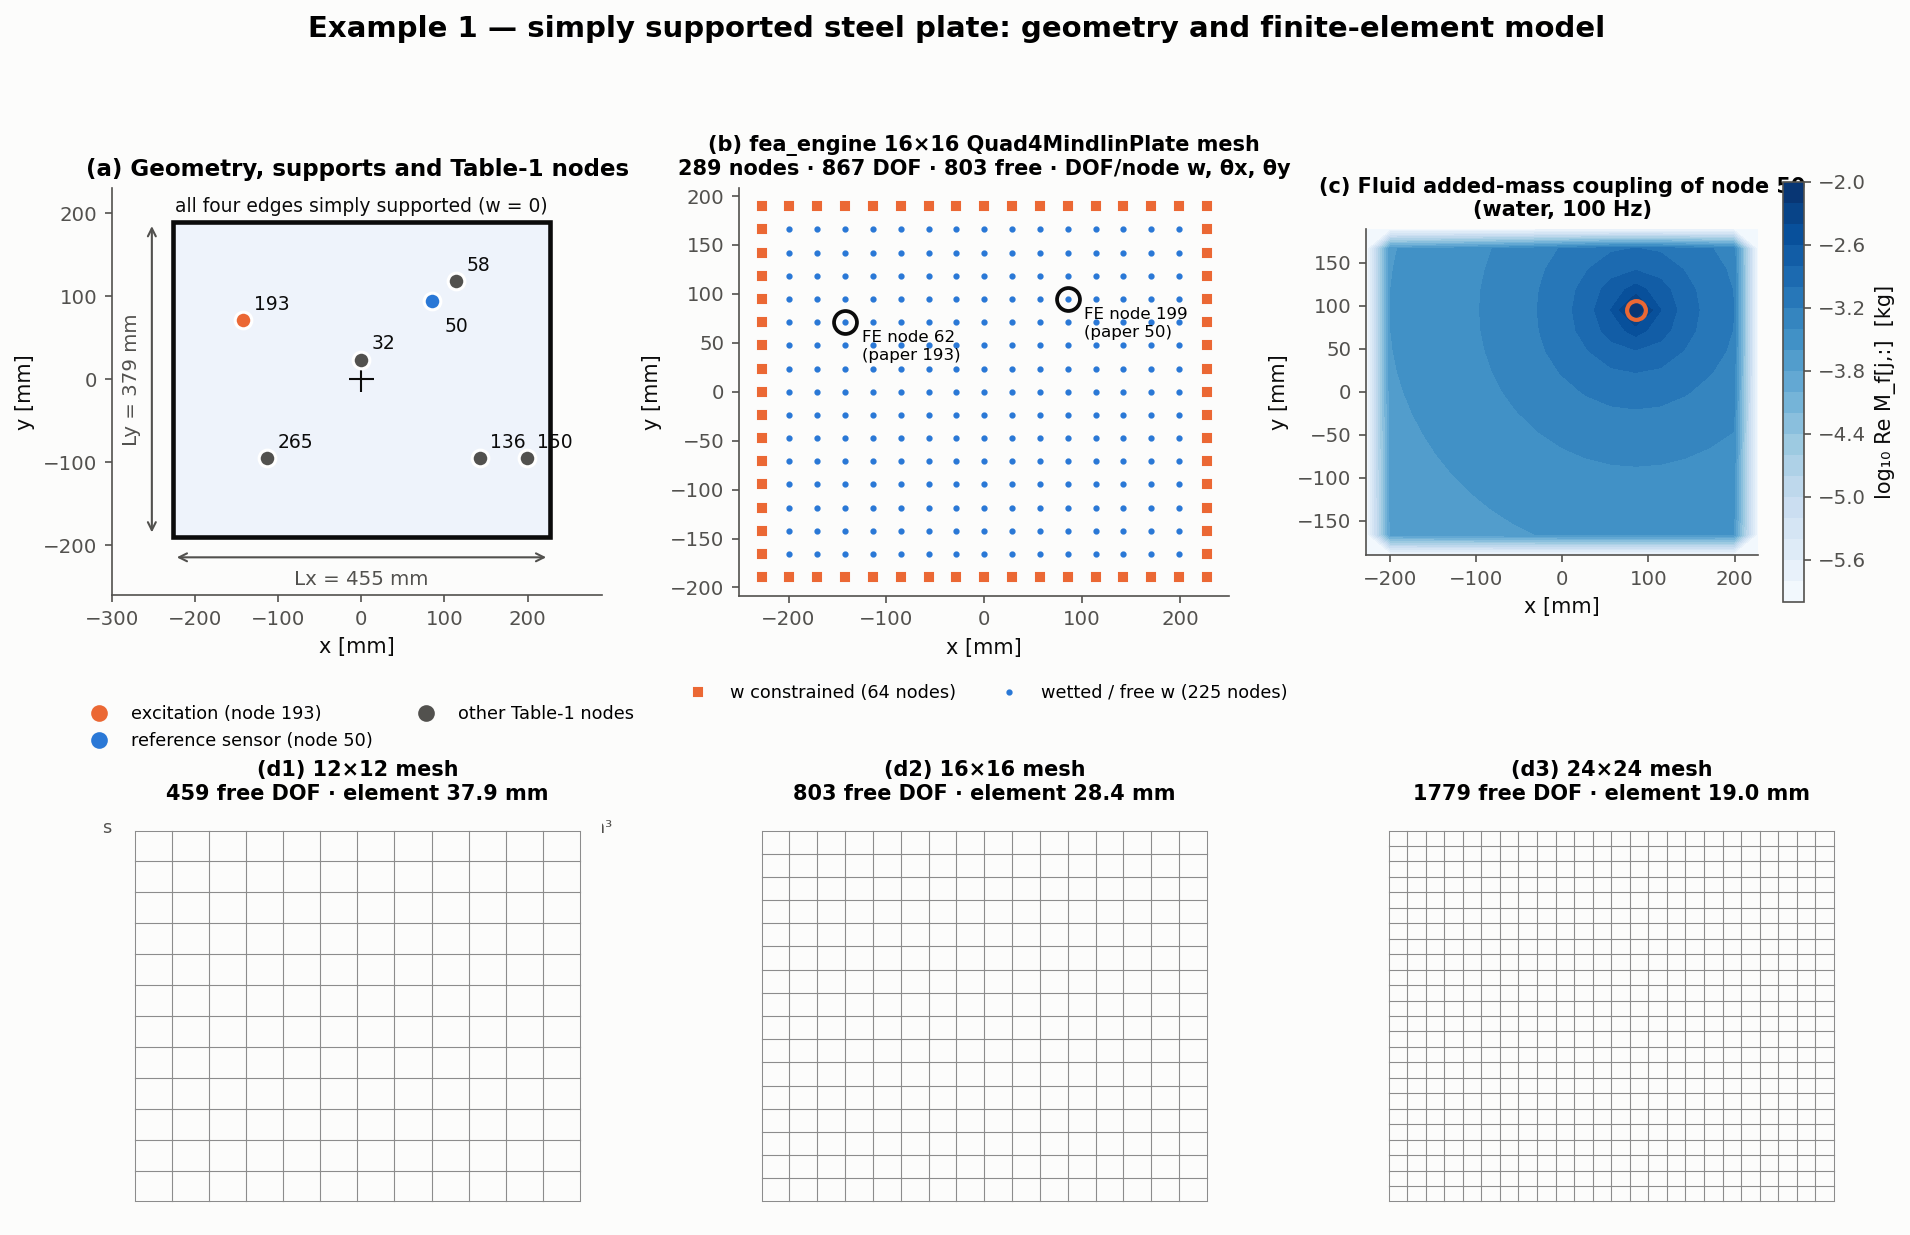
\includegraphics[width=0.98\linewidth]{figures/ch14r/fsi_geom.png}
\caption{Truth model of the identification study. (a) Plate, supports and the nodes of the publication's Table~1. (b) $16\times16$ Mindlin mesh with 64 constrained and 225 wetted nodes. (c) Real part of one row of the fluid added-mass matrix for water at 100~Hz; the coupling decays with distance from the source node. (d) The $12\times12$, $16\times16$ and $24\times24$ meshes of the mesh study.}\label{fig:vf-fsi-geom}
\end{figure}

\begin{figure}[tbp]
\centering
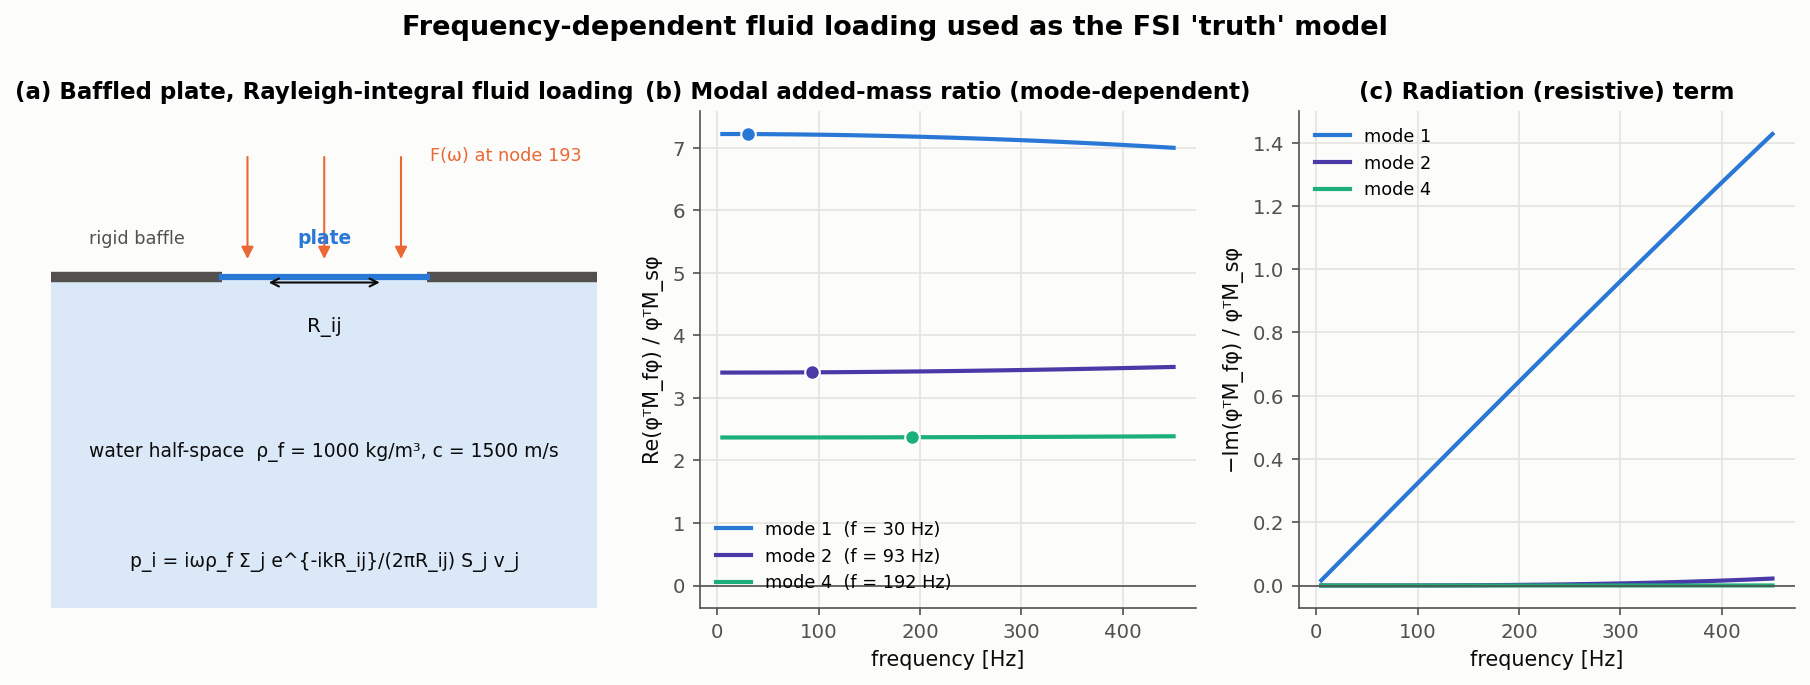
\includegraphics[width=0.9\linewidth]{figures/ch14r/fsi_fluid.png}
\caption{Frequency-dependent fluid loading. The modal added-mass ratio differs strongly by mode (about 7.2 for mode 1, 3.4 for mode 2, 2.4 for mode 4), so a uniform added mass cannot reproduce it; the radiation term grows with frequency and is largest for mode 1 (a monopole-like shape radiates efficiently).}\label{fig:vf-fsi-fluid}
\end{figure}

\begin{table}[tbp]
\centering\footnotesize
\caption{Set-up of the identification study.}\label{tab:vf-fsi-setup}
\begin{tabularx}{\linewidth}{@{}>{\raggedright\arraybackslash}p{3.2cm} >{\raggedright\arraybackslash}X@{}}
\toprule
Item & Value\\
\midrule
Plate & steel, $455\times379\times3$ mm; $E=2.1\times10^{11}$ Pa, $\nu=0.3$, $\rho_s=7850$ kg/m$^3$\\
Truth model & ANSYS finite element and boundary element model in the publication; here \texttt{Quad4MindlinPlate} 16$\times$16 and the Rayleigh-integral fluid mass\\
Sample grids, air & 17 + 17 points, 60:40:700 Hz and 80:40:720 Hz\\
Sample grids, water & 11 + 11 points, 10:40:410 Hz and 30:40:430 Hz\\
Screening & $N_{\rm ROM}=25$, $\varepsilon_f=0.5\,\%$, $\varepsilon_\eta=10\,\%$, $\tau_s=0.95$\\
Excitation / measurement cases & (1) excite 193, measure 50; (2) 193, 150; (3) 32, 58, 136, 193, 265 together, measure 50; (4) 150, 136\\
Fluid sides & one (the publication's plate is surrounded by fluid)\\
\bottomrule
\end{tabularx}
\end{table}

\Cref{fig:vf-fsi-frf} shows the only data given to the identification: the markers on the two interleaved grids against the full FRF, which the method never sees.

\begin{figure}[tbp]
\centering
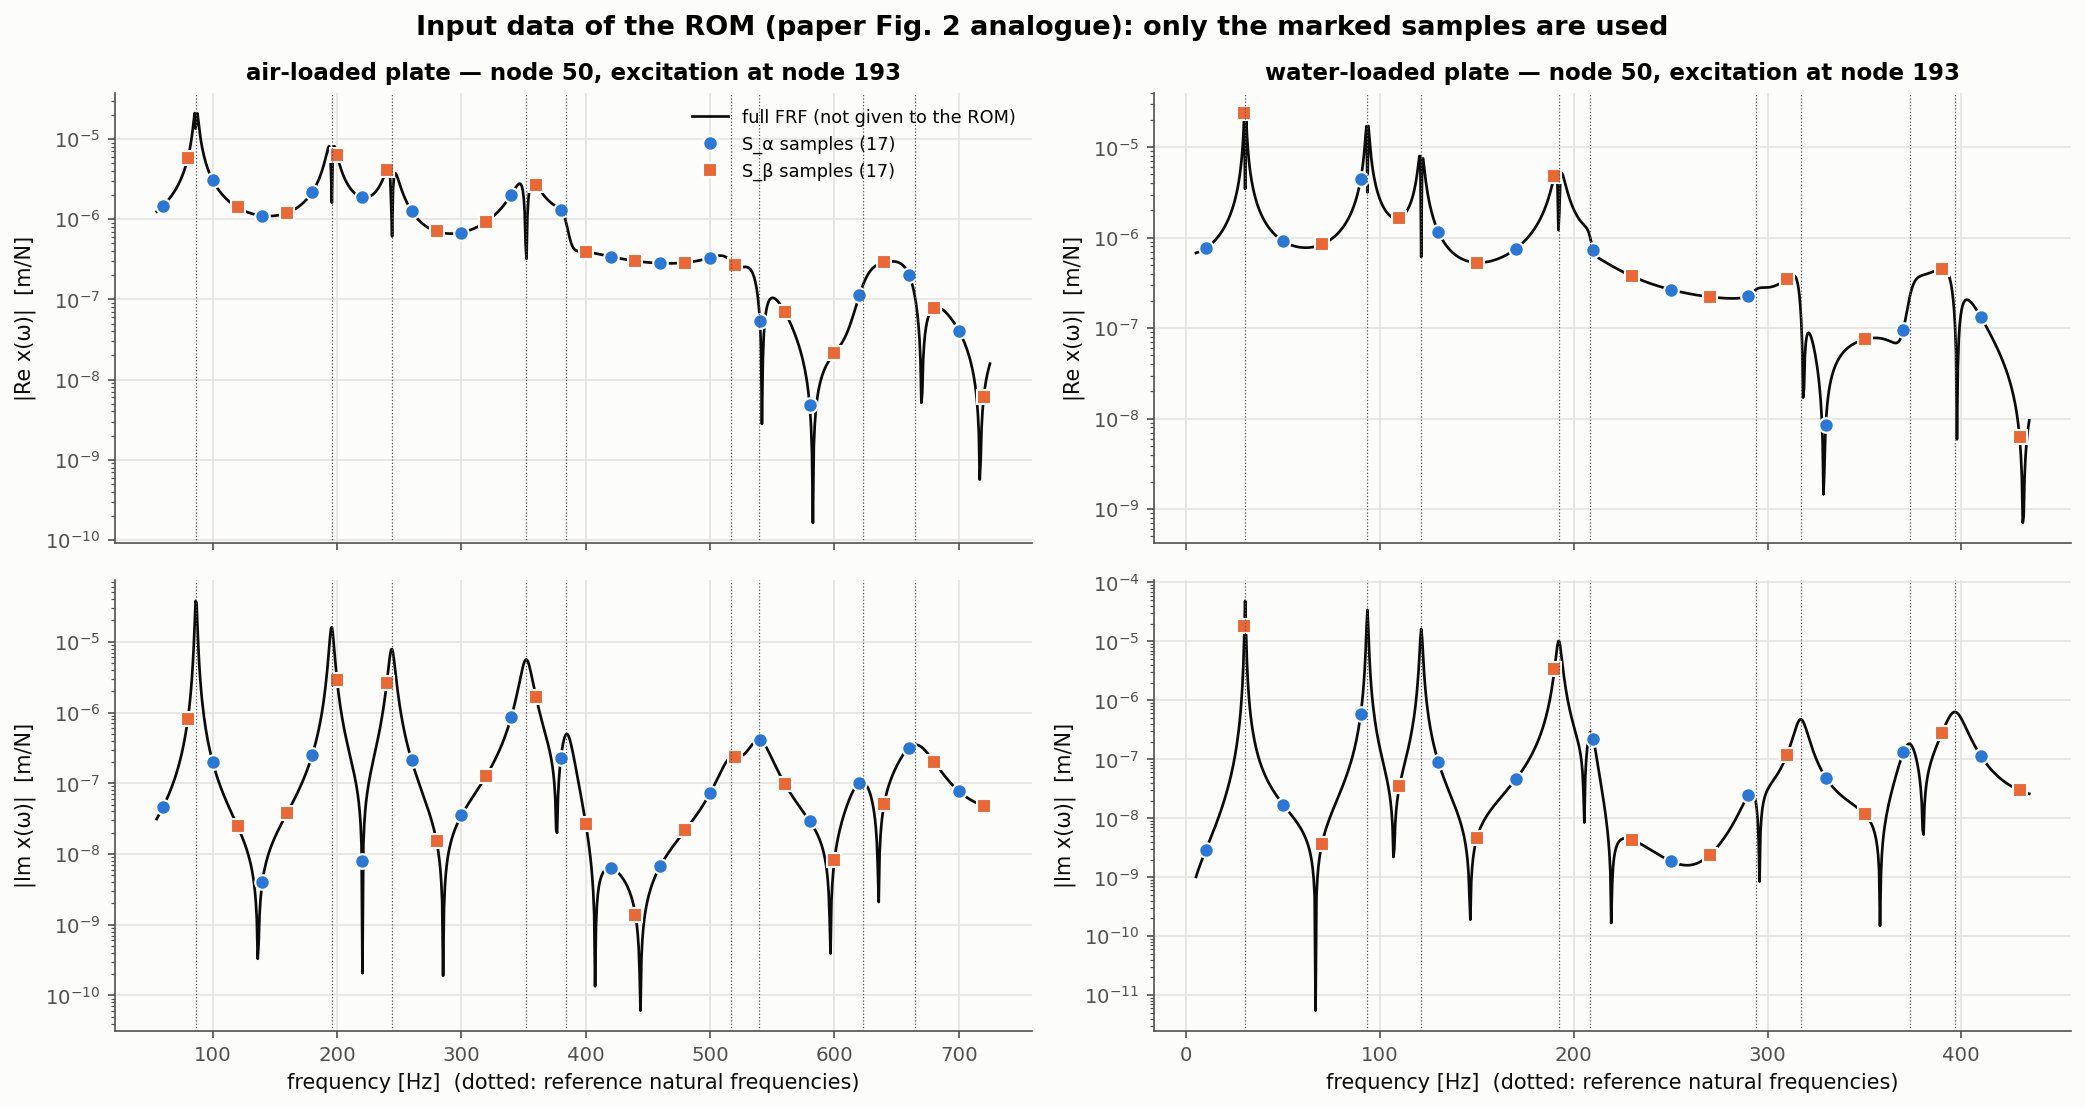
\includegraphics[width=0.9\linewidth]{figures/ch14r/fsi_frf.png}
\caption{Analogue of the publication's Fig.~2: the full FRF at node 50 for excitation at node 193 (black, not given to the method) and the samples used, on the interleaved grids (circles and squares); dotted lines are the reference natural frequencies.}\label{fig:vf-fsi-frf}
\end{figure}

\subsection*{Results: truth model against the publication (S1)}

\Cref{fig:vf-fsi-table2} compares the frequency deviation and damping ratio of the truth model with the publication's Table~2. In air the frequencies lie within $-0.3$ to $+7.2\,\%$ of the published ones ($\le1.7\,\%$ for modes 1--4) and the damping within $0.03$--$0.18$ points. In water the frequencies lie within $-9.3\,\%$ (mode 1) and $-1.1$ to $-5.0\,\%$ (modes 2--9); an earlier model with a uniform added mass was $-15$ to $-48\,\%$ off. The damping of water modes 2, 3, 4, 7, 8, 9 matches closely (mode 3: $0.570$ against $0.584$; mode 9: $1.548$ against $1.564$) but not mode 1 ($0.945$ against $0.336$), mode 5 ($1.267$ against $0.625$) or mode 6 ($1.592$ against $1.158$). The remaining differences come from model differences (Mindlin quadrilaterals against the publication's ANSYS model, a baffled half-space against its boundary-element treatment, one-sided wetting); the absolute numbers below should therefore not be compared with the publication's tables, only the behaviour of the method.

\begin{figure}[tbp]
\centering
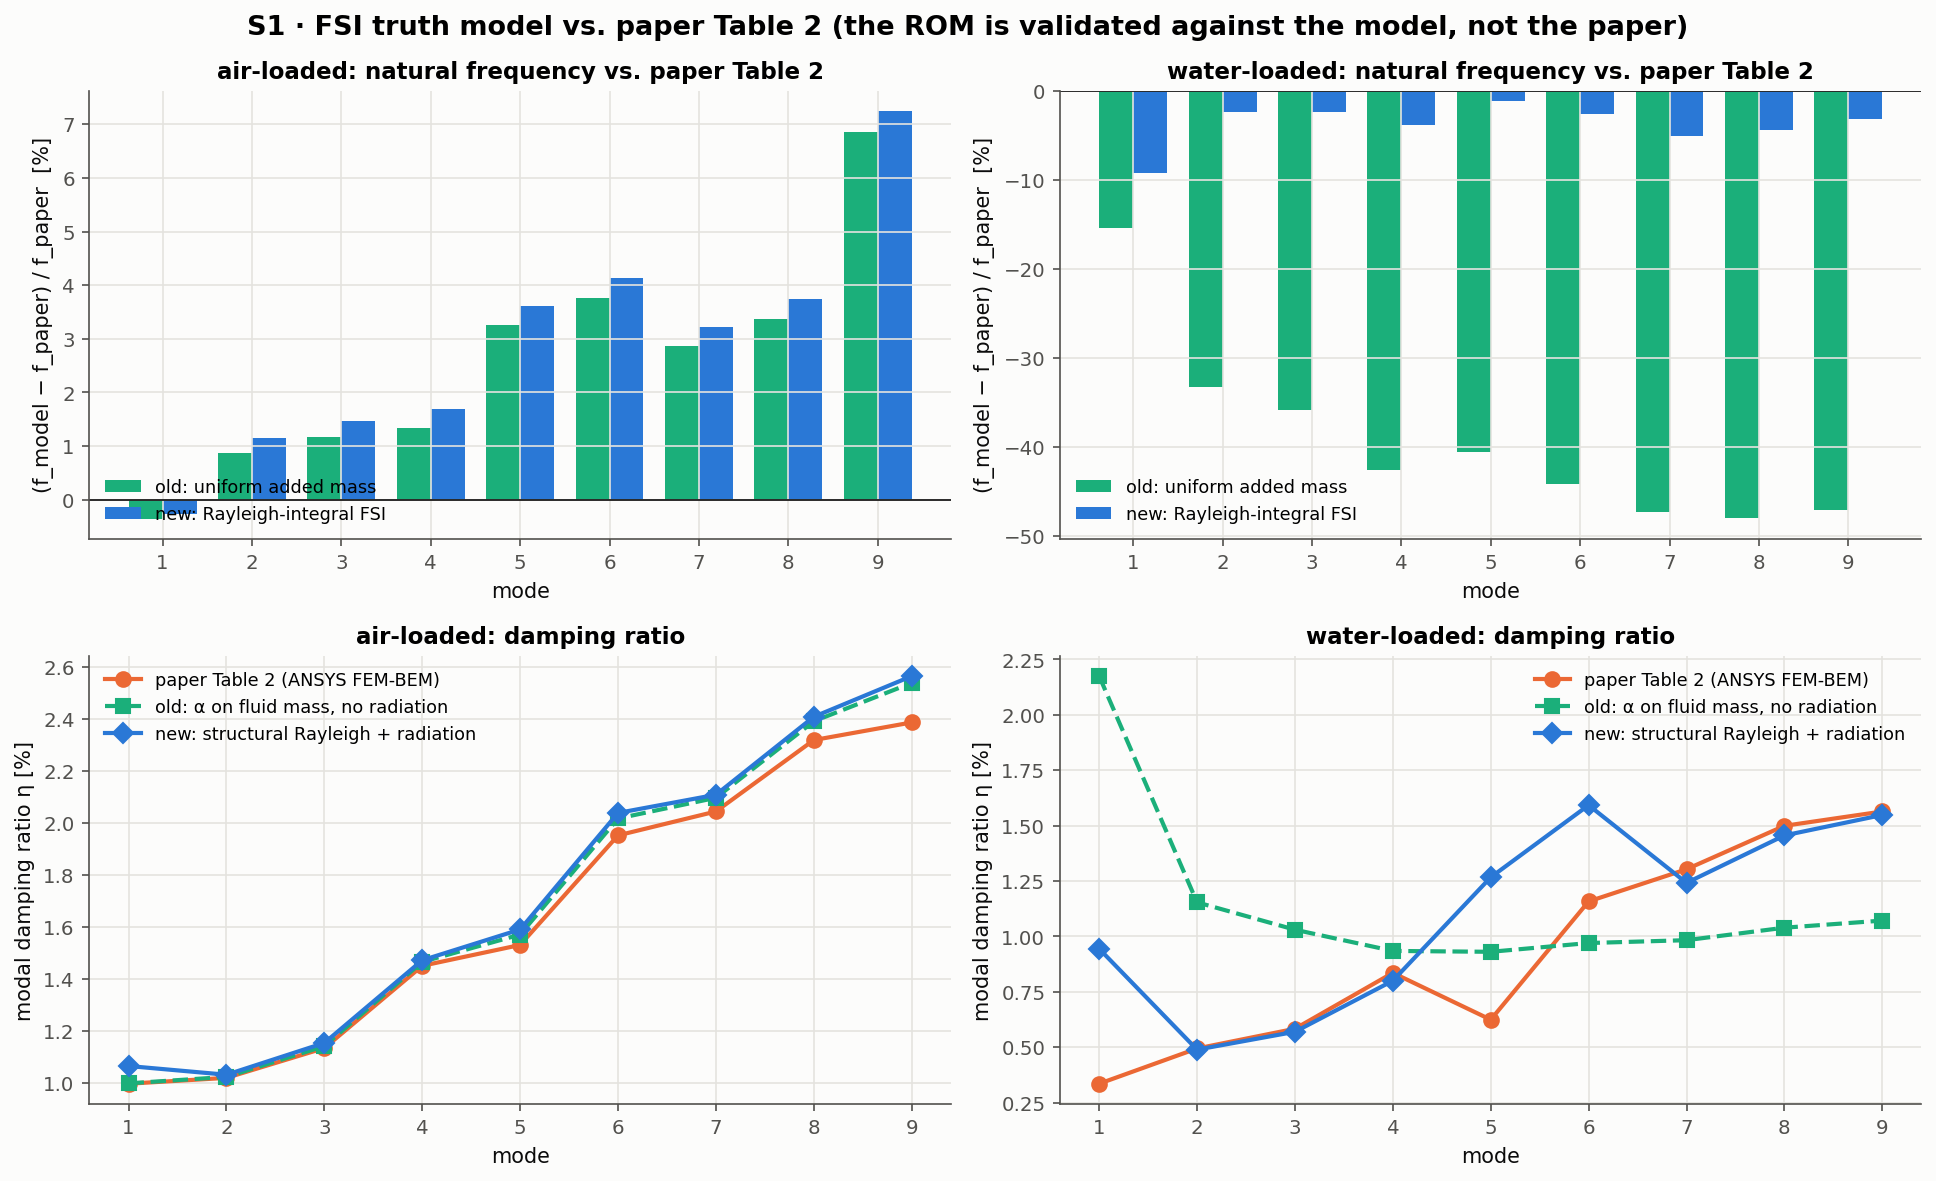
\includegraphics[width=0.9\linewidth]{figures/ch14r/fsi_table2.png}
\caption{Frequency deviation and damping ratio of the truth model against the publication's Table~2, air and water. Green: the earlier uniform-added-mass model; blue: the Rayleigh-integral model used for all studies.}\label{fig:vf-fsi-table2}
\end{figure}

\subsection*{Results: mesh, boundary condition and excitation (S2--S4)}

\emph{Mesh (S2).} \Cref{tab:vf-fsi-mesh} gives the largest ROM--FE error for three meshes in air; the publication reports below $0.2\,\%$. The method reproduces whatever mesh it is given to near round-off, because the air-loaded system is effectively frequency-independent in the band; the mode-1 frequency moves from 86.78 to 86.63 to 86.48~Hz over the meshes, which is a property of the finite element model and not of the identification.

\begin{table}[tbp]
\centering\footnotesize
\caption{Largest difference between identified and finite element frequency and damping (air).}\label{tab:vf-fsi-mesh}
\begin{tabular}{@{}lrrl@{}}
\toprule
Mesh & Frequency error & Damping error & Publication\\
\midrule
$12\times12$ & $6.7\times10^{-8}\,\%$ & $7.0\times10^{-6}\,\%$ & $<0.2\,\%$\\
$16\times16$ & $7.7\times10^{-8}\,\%$ & $6.6\times10^{-6}\,\%$ & $<0.2\,\%$\\
$24\times24$ & $4.4\times10^{-7}\,\%$ & $7.9\times10^{-6}\,\%$ & $<0.2\,\%$\\
\bottomrule
\end{tabular}
\end{table}

\begin{figure}[tbp]
\centering
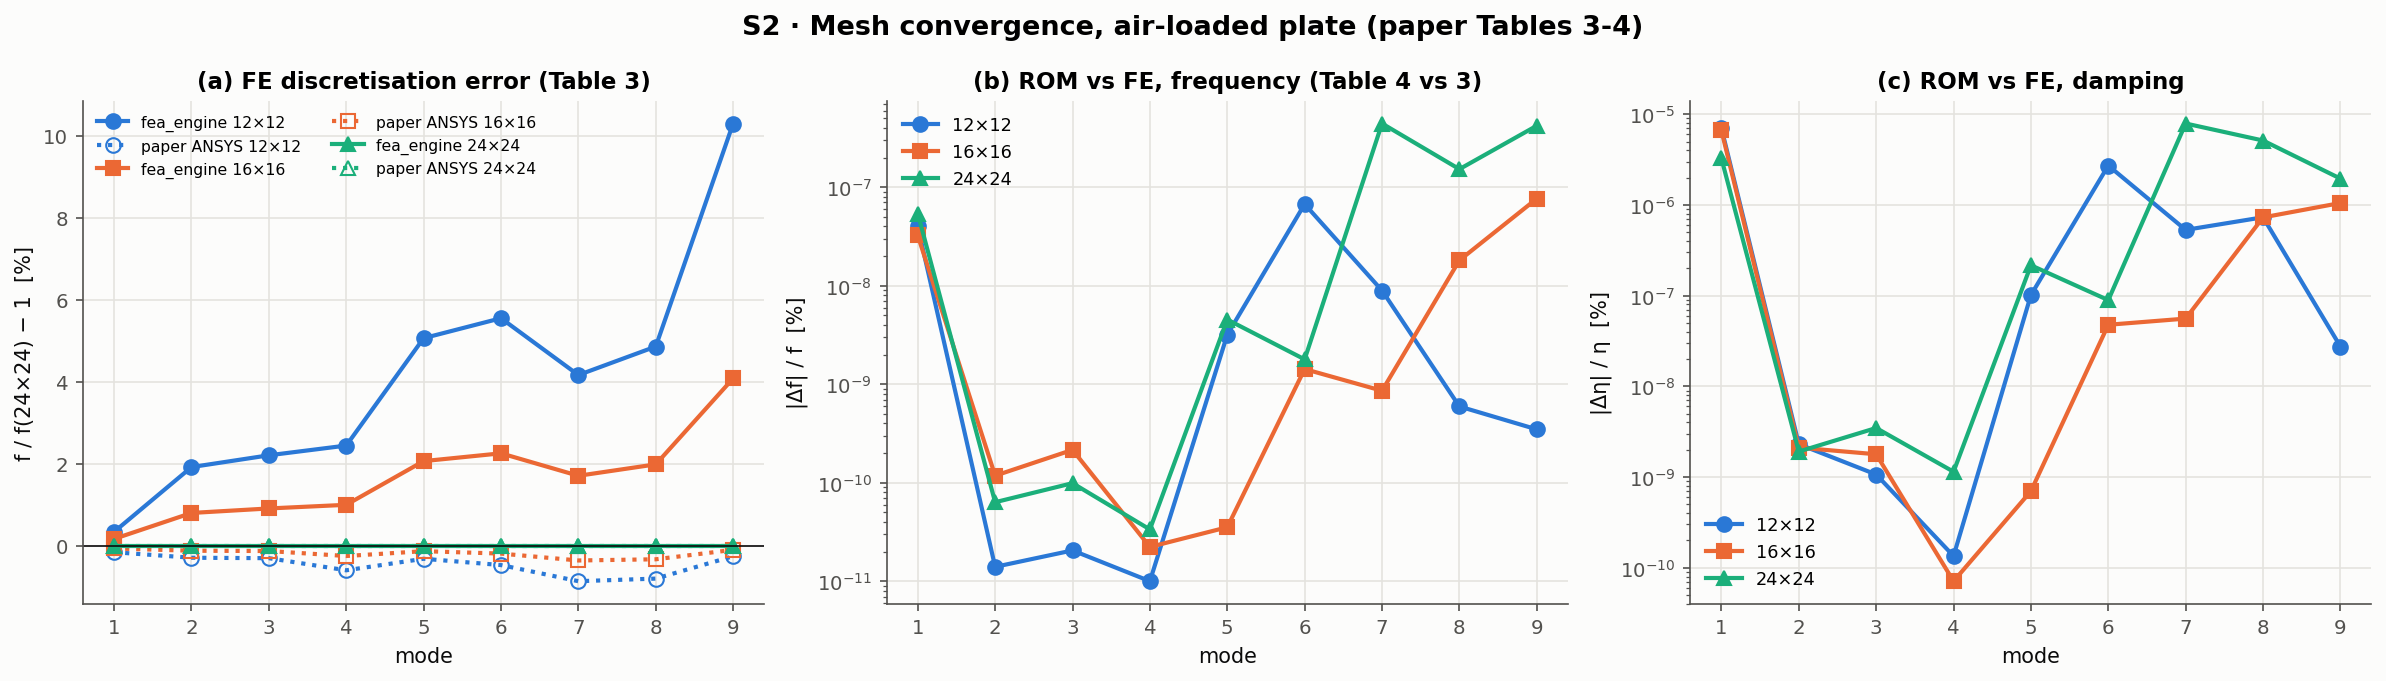
\includegraphics[width=0.9\linewidth]{figures/ch14r/fsi_mesh.png}
\caption{Reference (finite element) and identified frequency and damping for the three meshes.}\label{fig:vf-fsi-mesh}
\end{figure}

\emph{Boundary condition (S3).} For simply supported and clamped plates all nine modes are recovered with $e_f<10^{-7}\,\%$ and $e_\eta<2\times10^{-6}\,\%$; the clamped plate has mode 1 at 160.9~Hz (publication 159.5~Hz) and mode 9 at 854.7~Hz (777.5~Hz, $+9.9\,\%$). The publication's second variant with triangular shells is not covered, because the package has no triangular plate-bending element.

\emph{Excitation and measurement (S4).} \Cref{tab:vf-fsi-cases} and \Cref{fig:vf-fsi-cases} give the four configurations. Results do not depend on where the force is applied or the response measured, consistent with the publication's claim of excitation-independent identification. The $10^4$--$10^5$ times larger water error has a clear cause: the fluid mass and radiation damping of the truth model vary with frequency, so $x(\omega)$ is only approximately rational in $\omega^2$ and the pencil is no longer exact. The publication's low-error claim for water is therefore reproduced only at the $0.01$--$0.2\,\%$ (frequency) level.

\begin{table}[tbp]
\centering\footnotesize
\caption{Identification over the four excitation--measurement cases.}\label{tab:vf-fsi-cases}
\begin{tabular}{@{}lrrrrrr@{}}
\toprule
Fluid & Detected & Mean $e_f$ & Max $e_f$ & Mean $e_\eta$ & Max $e_\eta$ & Non-physical\\
\midrule
Air, all 4 cases & 9/9 & $\le7.3\times10^{-7}\,\%$ & $6.5\times10^{-6}\,\%$ & $\le2.0\times10^{-5}\,\%$ & $1.7\times10^{-4}\,\%$ & 0\\
Water, all 4 cases & 9/9 & $4.9\times10^{-3}$--$3.3\times10^{-2}\,\%$ & $0.19\,\%$ & $0.85$--$0.91\,\%$ & $4.5\,\%$ & 0\\
\bottomrule
\end{tabular}
\end{table}

\begin{figure}[tbp]
\centering
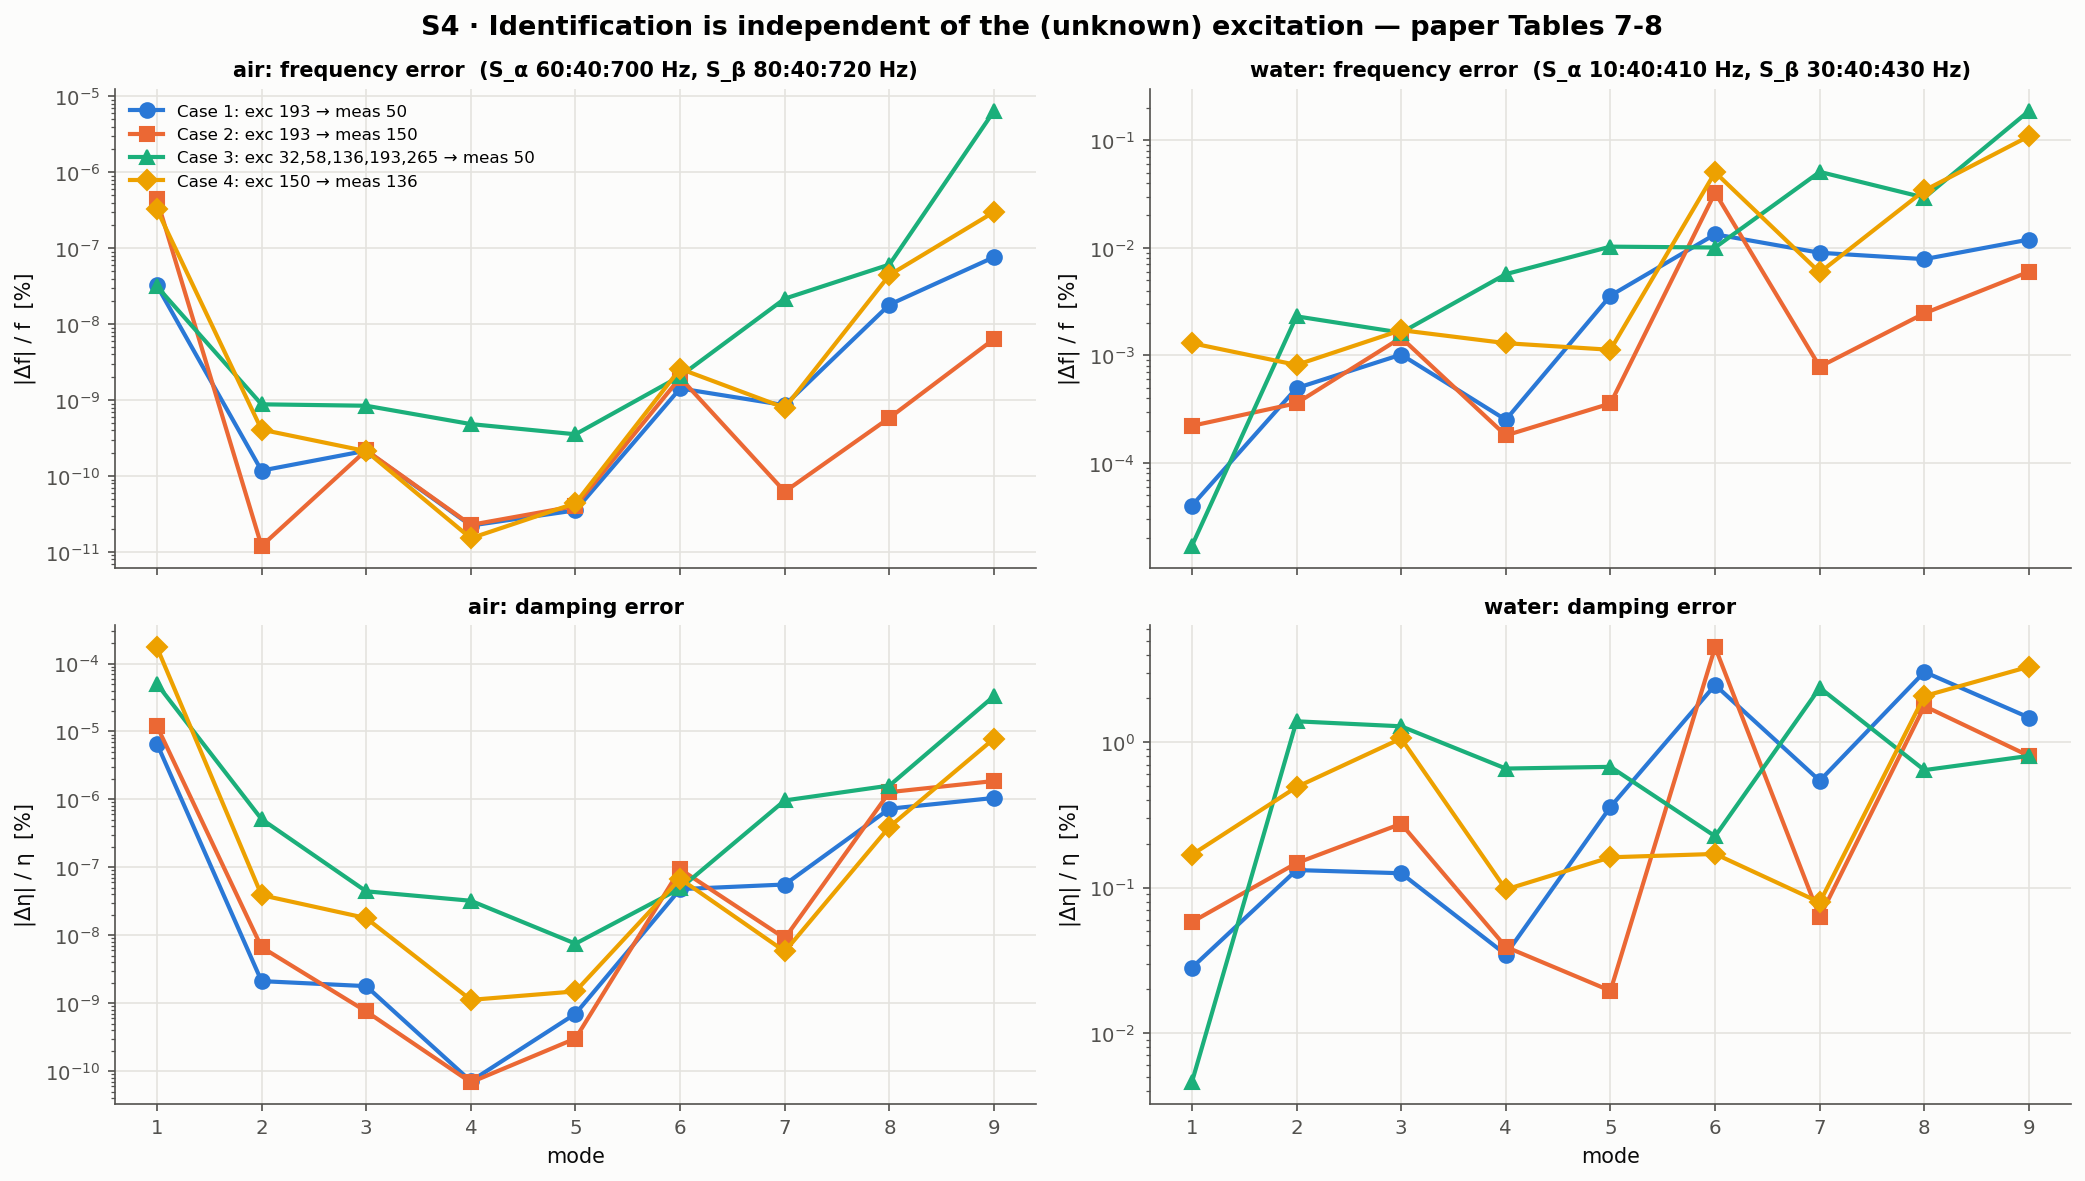
\includegraphics[width=0.98\linewidth]{figures/ch14r/fsi_cases.png}
\caption{Frequency and damping error for the four excitation--measurement configurations; left air, right water.}\label{fig:vf-fsi-cases}
\end{figure}

\subsection*{Results: sensitivity and noise (S5, S6)}

\emph{Sensitivity (water).} \Cref{fig:vf-fsi-sens} gives the mean error against (a) interpolation density, (b) frequency band, (c) sensor position and (d) excitation pattern. Errors fall monotonically as the grid is refined: mean $e_f$ is $0.36\,\%$ (18 points), $5.3\times10^{-3}\,\%$ (22), $6.0\times10^{-5}\,\%$ (26) and $1.1\times10^{-6}\,\%$ (36); with 18 points only 5 of 9 modes are detected and two spurious eigenpairs appear, and the publication's grid (22 points) gives 9 of 9 in a single model but only 5 of 9 after default screening. The wide band 0--500~Hz gives 9 of 9 even after screening, while an upper limit of 397~Hz, just below the ninth mode, loses modes (3 of 9 screened, $e_\eta\approx19\,\%$). Sensors at an edge midpoint or the plate centre detect only 6 and 3 of 9 modes, because they lie on nodal lines of the antisymmetric modes, while a corner sensor sees all nine; the modes that are seen are extremely accurate ($e_f\sim10^{-5}\,\%$). In-phase multi-point excitation leaves 1 of 9 modes after screening (single-model detection is still 9 of 9), random-phase multi-point excitation gives 6 of 9 with one spurious mode; a single point force is the most favourable pattern.

\begin{figure}[tbp]
\centering
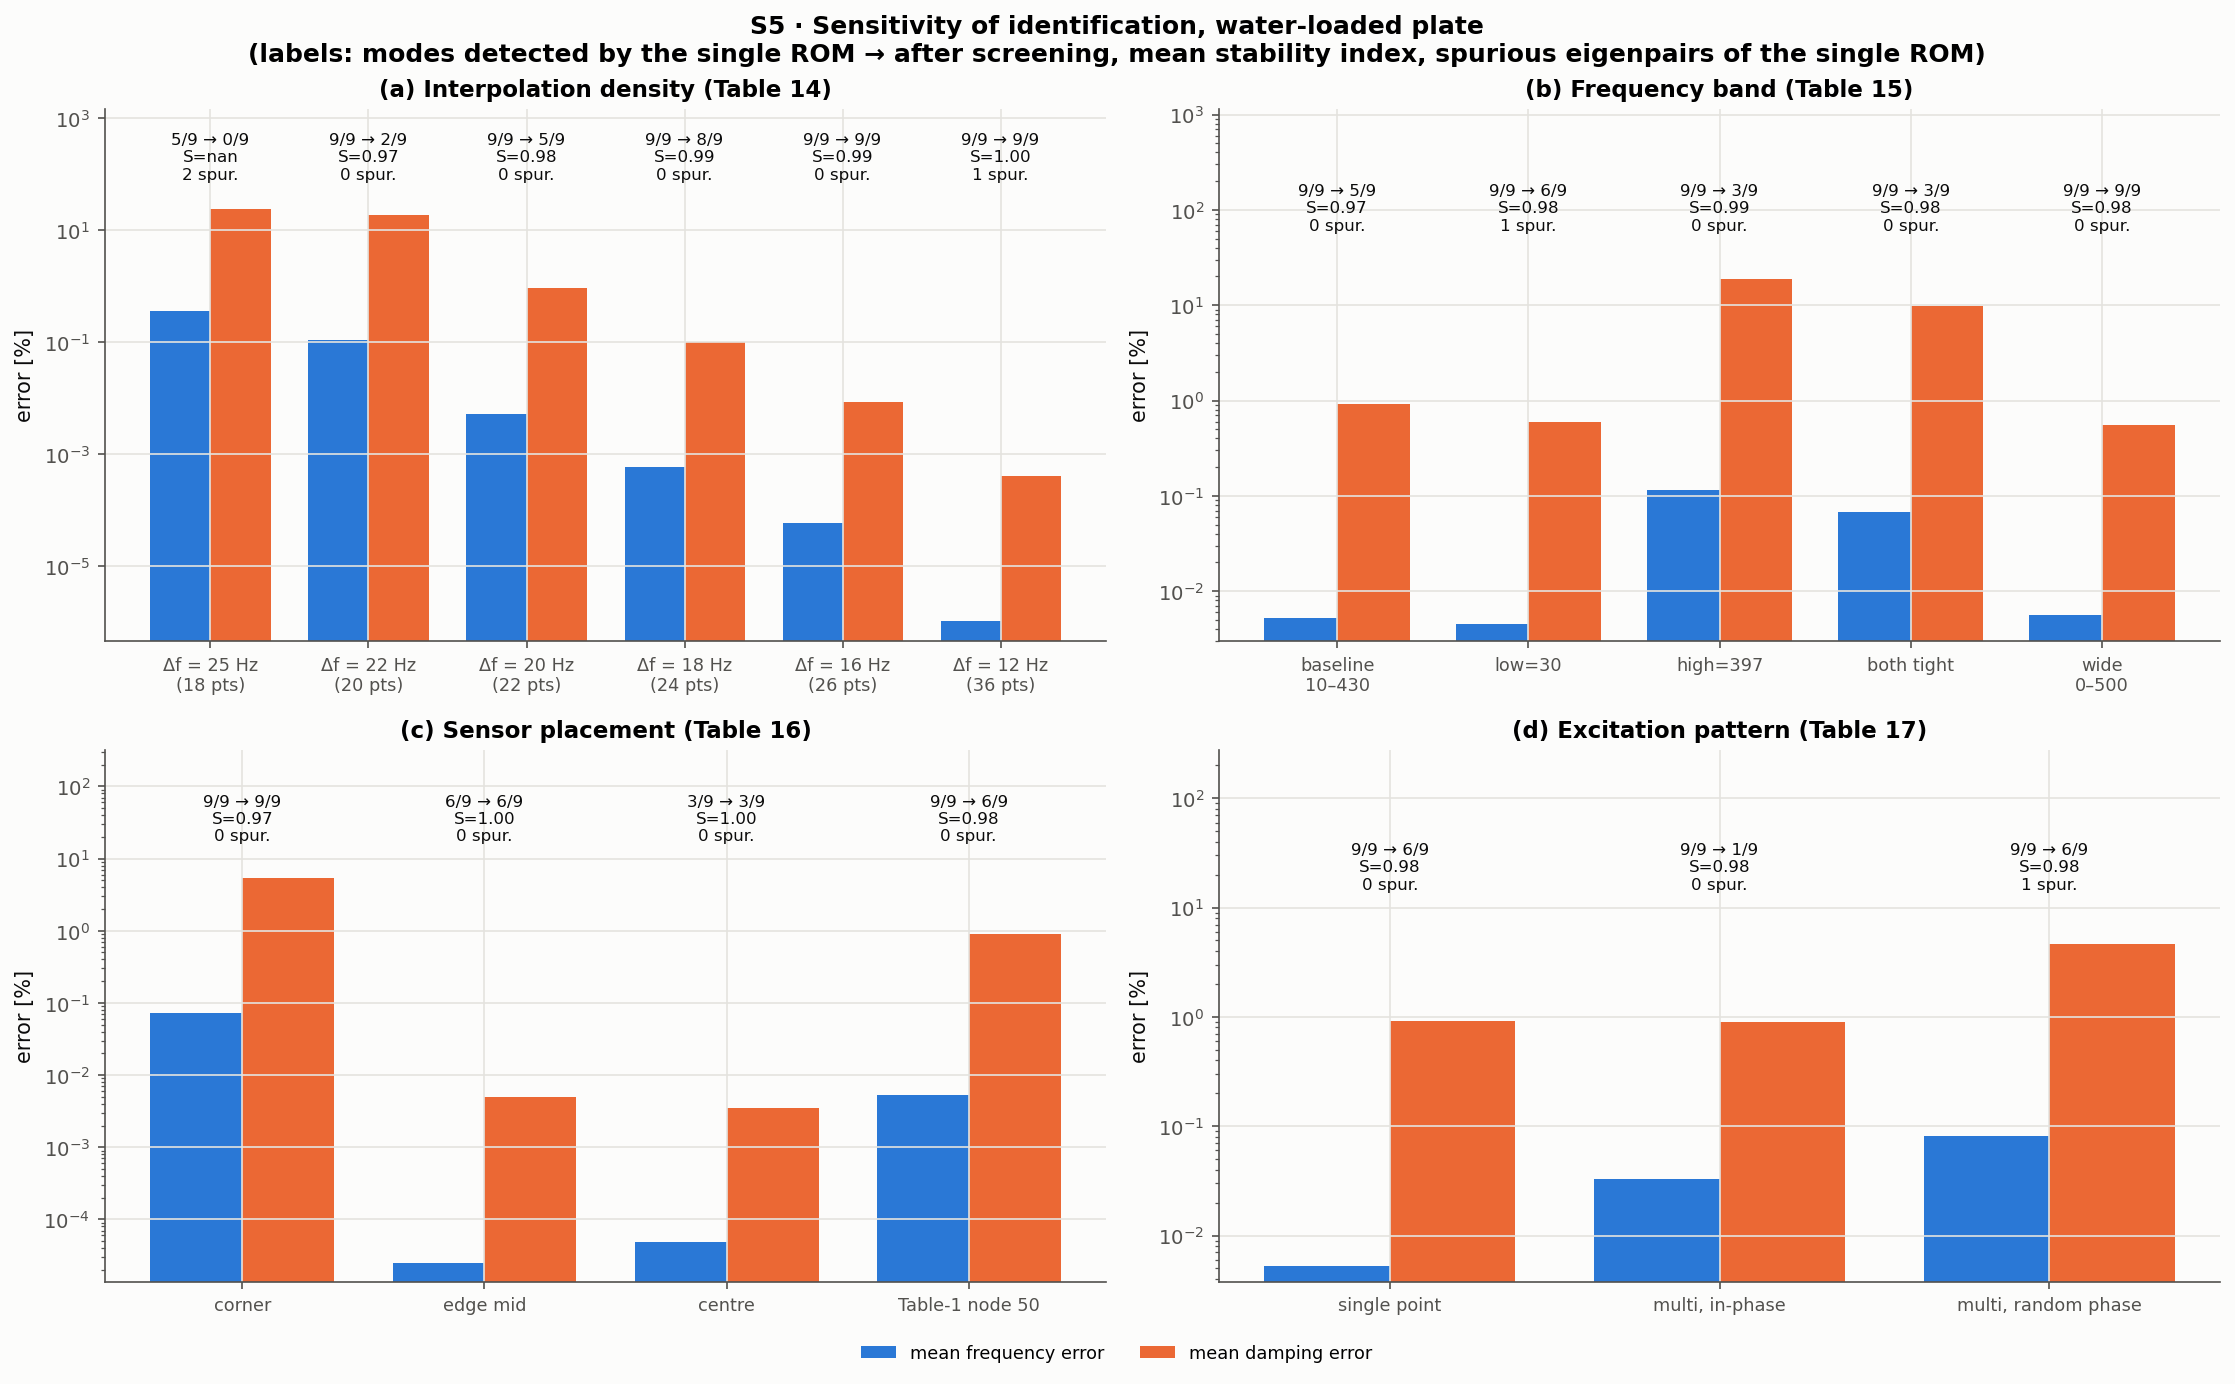
\includegraphics[width=0.98\linewidth]{figures/ch14r/fsi_sens.png}
\caption{Mean frequency (blue) and damping (orange) error against (a) interpolation density, (b) band, (c) sensor position, (d) excitation pattern, water. Labels give modes detected by a single model, after screening, the mean stability index and the number of spurious eigenpairs.}\label{fig:vf-fsi-sens}
\end{figure}

\emph{Noise.} \Cref{tab:vf-fsi-noise} and \Cref{fig:vf-fsi-noise} give median errors over 20 noise realisations per signal-to-noise ratio (SNR, 11 + 11 samples). Frequencies degrade gracefully (about $1\,\%$ even at 20~dB for the worst mode); damping is far more fragile, with errors above $10\,\%$ below about 60~dB. Screening never produced a spurious mode on the dense pool (zero at all noise levels), but at low noise ratios it also accepts almost nothing: the default thresholds ($\varepsilon_\eta=10\,\%$, $\tau_s=0.95$) were tuned on clean data, and under noise the damping scatter between models exceeds $10\,\%$, so physical modes are rejected. A noise-dependent tolerance would be needed in practice.

\begin{table}[tbp]
\centering\footnotesize
\caption{Noise robustness, water.}\label{tab:vf-fsi-noise}
\begin{tabular}{@{}rrrrrr@{}}
\toprule
SNR & Mean $e_f$ & Mean $e_\eta$ & Detected (single) & Spurious (single) & Detected (screened, 85-sample pool)\\
\midrule
20 dB & $0.90\,\%$ & $379\,\%$ & 2.7 & 3.9 & 0.0\\
40 dB & $0.67\,\%$ & $49\,\%$ & 5.3 & 2.6 & 0.3\\
60 dB & $0.27\,\%$ & $26\,\%$ & 8.0 & 1.2 & 1.8\\
80 dB & $0.06\,\%$ & $4.2\,\%$ & 9.0 & 0.2 & 6.2\\
\bottomrule
\end{tabular}
\end{table}

\begin{figure}[tbp]
\centering
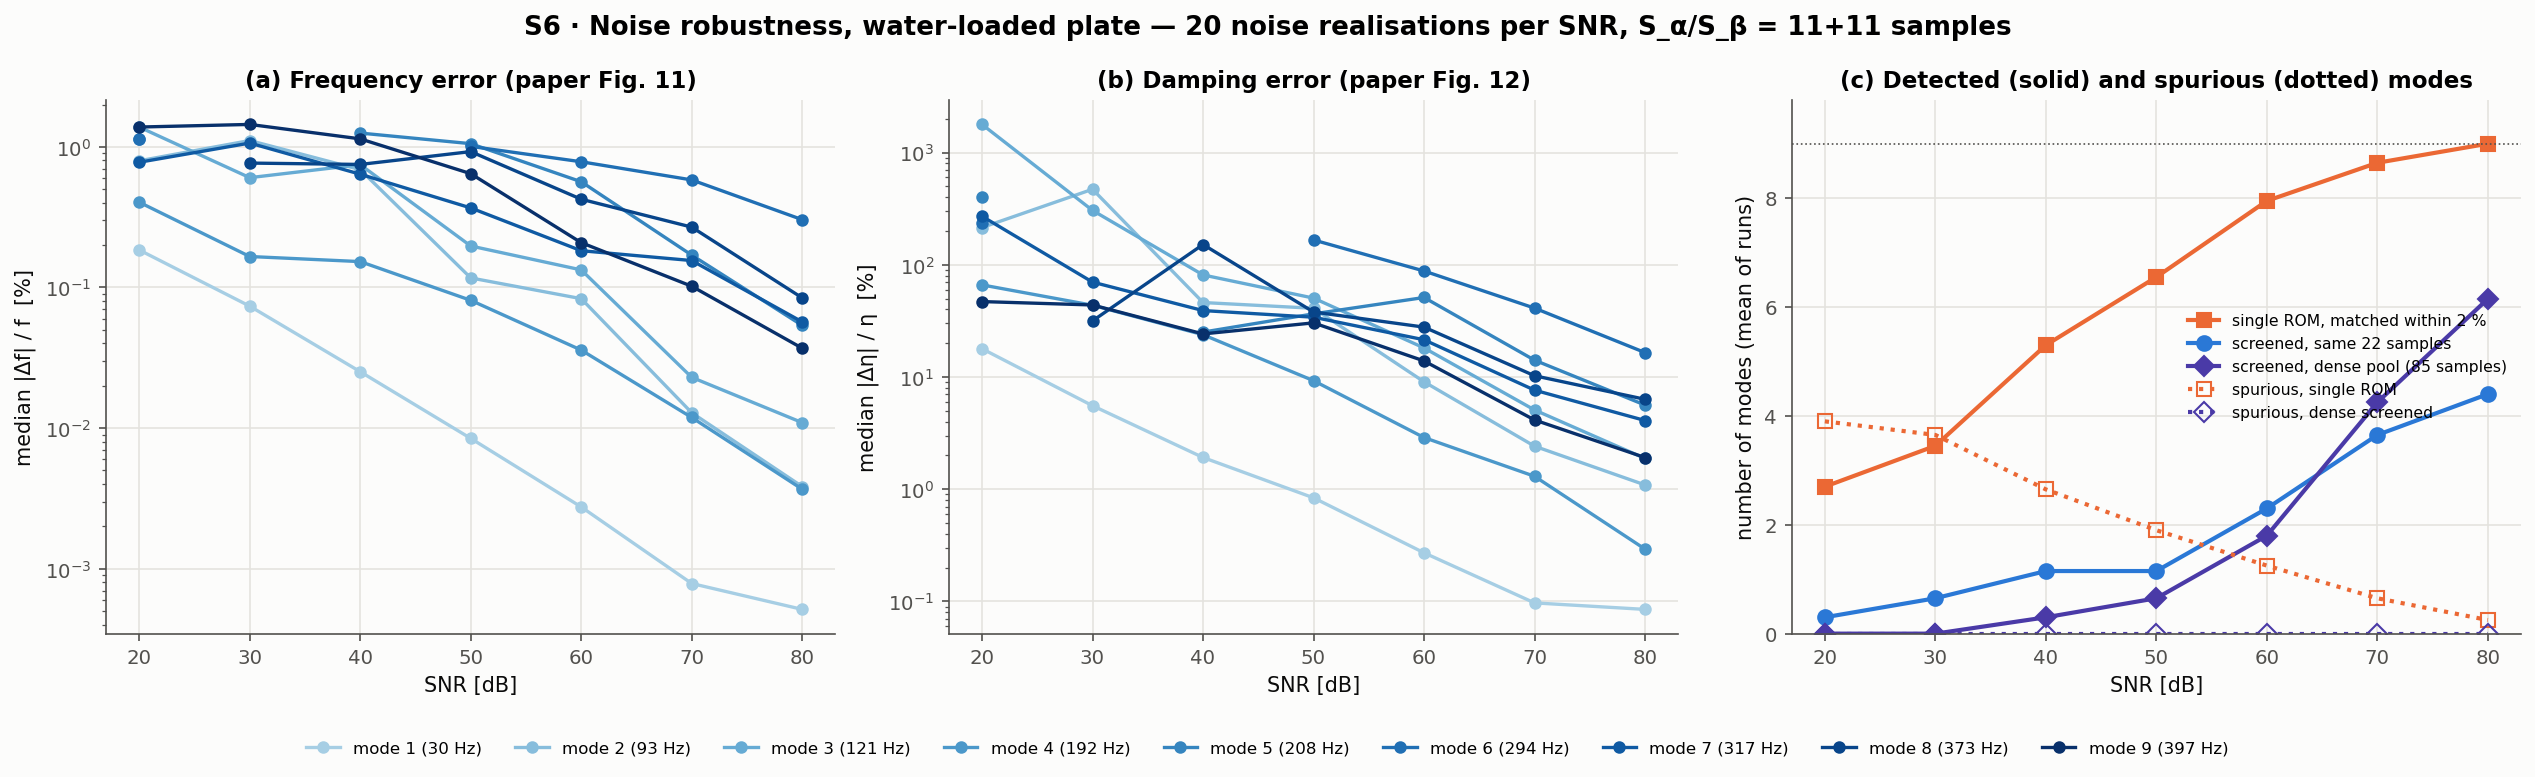
\includegraphics[width=0.98\linewidth]{figures/ch14r/fsi_noise.png}
\caption{Median error over 20 noise realisations per SNR: (a) frequency, (b) damping per mode, (c) detected (solid) and spurious (dotted) modes for a single model and for screening on 22 or 85 samples.}\label{fig:vf-fsi-noise}
\end{figure}

\subsection*{Results: mode shapes (S7)}

\Cref{tab:vf-fsi-mac} and \Cref{fig:vf-fsi-shapes,fig:vf-fsi-mac} give the shapes reconstructed as $\boldsymbol\Phi=\mathbf X_\beta\tilde\Phi$, scored by \cref{eq:fsi-mac} against the finite element shapes of the water-loaded plate. Seven of nine modes have MAC above $0.999$ on the publication-sized grid and all nine reach at least $0.9999$ on a denser $14+14$ grid; the weakest are modes 6 and 8 ($0.953$, $0.984$) and the largest off-diagonal MAC is $0.021$, so the recovered shapes are well separated. The reconstruction is real-normalised, phase-aligned and averaged over the ensemble, because the eigenvector of a single model can be badly conditioned even when its eigenvalue is accurate.

\begin{table}[tbp]
\centering\footnotesize
\caption{Mode shapes of the water-loaded plate.}\label{tab:vf-fsi-mac}
\begin{tabular}{@{}rrrrrr@{}}
\toprule
Mode & $f_{\rm ref}$ (Hz) & $f_{\rm id}$ (Hz) & MAC, 11+11 & MAC, 14+14 & Max off-diagonal\\
\midrule
1 & 30.37 & 30.37 & 1.0000 & 1.0000 & 0.017\\
2 & 93.45 & 93.45 & 0.9999 & 1.0000 & 0.006\\
3 & 121.24 & 121.24 & 0.9999 & 1.0000 & 0.001\\
4 & 192.21 & 192.21 & 1.0000 & 1.0000 & 0.000\\
5 & 208.42 & 208.41 & 0.9999 & 1.0000 & 0.017\\
6 & 293.91 & 293.95 & 0.9532 & 0.9999 & 0.021\\
7 & 317.10 & 317.07 & 0.9999 & 1.0000 & 0.001\\
8 & 373.24 & 373.21 & 0.9842 & 1.0000 & 0.004\\
9 & 396.57 & 396.52 & 0.9993 & 1.0000 & 0.006\\
\bottomrule
\end{tabular}
\end{table}

\begin{figure}[tbp]
\centering
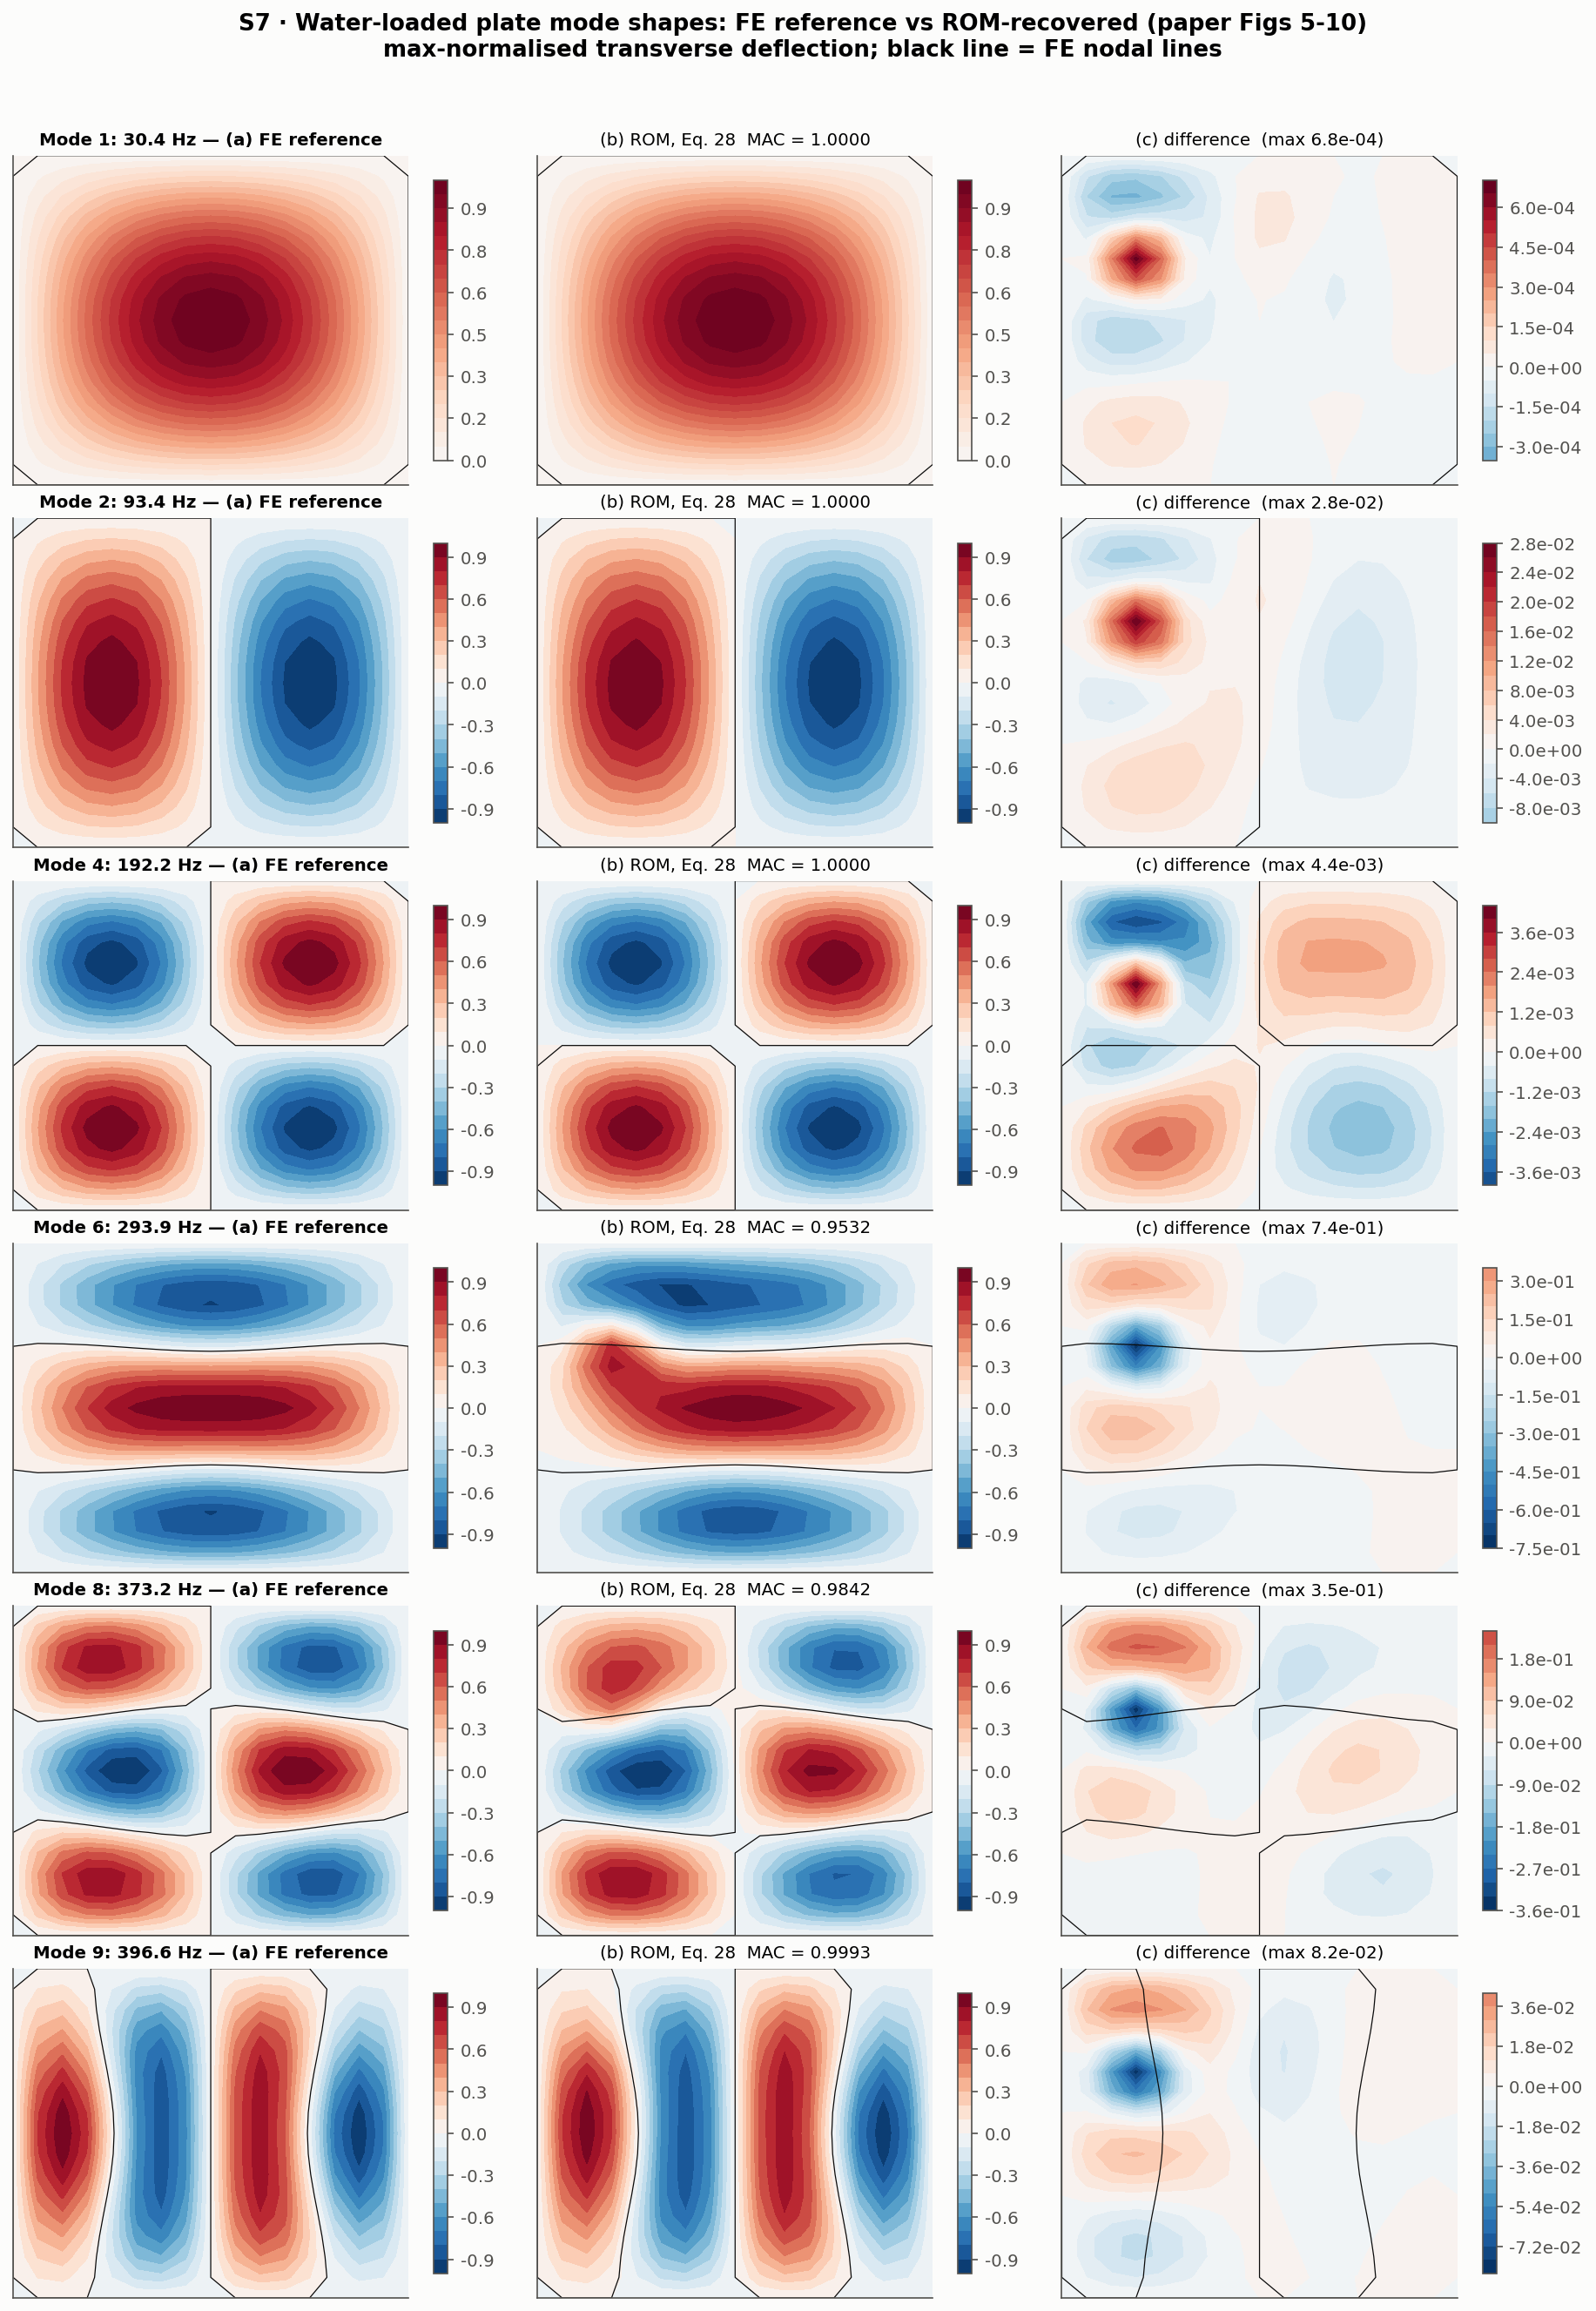
\includegraphics[width=0.98\linewidth]{figures/ch14r/fsi_shapes.png}
\caption{Identified mode shapes against finite element reference shapes, water-loaded plate.}\label{fig:vf-fsi-shapes}
\end{figure}

\begin{figure}[tbp]
\centering
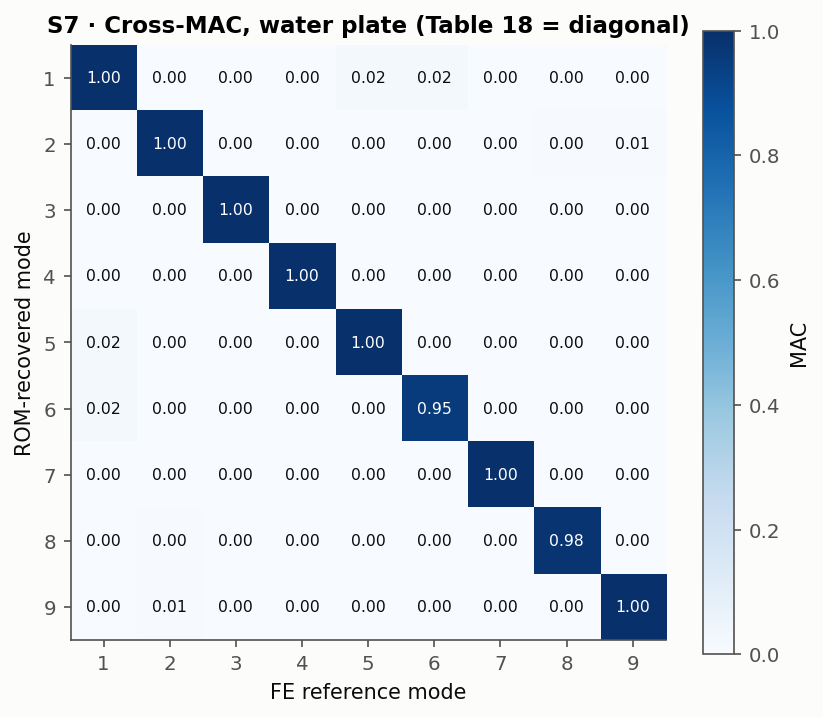
\includegraphics[width=0.6\linewidth]{figures/ch14r/fsi_mac.png}
\caption{Cross-MAC between identified and reference modes (11+11 grid); the diagonal is the publication's Table~18.}\label{fig:vf-fsi-mac}
\end{figure}

\subsection*{Comparison with the publication}

\begin{table}[tbp]
\centering\footnotesize
\caption{Claims of \citet{liu2026fsi} and the outcome against the author's own truth model.}\label{tab:vf-fsi-cmp}
\begin{tabularx}{\linewidth}{@{}>{\raggedright\arraybackslash}p{4.0cm} >{\raggedright\arraybackslash}X >{\raggedright\arraybackslash}p{2.3cm}@{}}
\toprule
Claim & This work & Outcome\\
\midrule
Frequencies and damping in air, any mesh and boundary (Tables 3--6) & errors $\lesssim10^{-5}\,\%$ & reproduced\\
Excitation- and sensor-independent identification (Tables 7--8) & 9/9 modes in all four cases; air $\le6.5\times10^{-6}\,\%$, water $\le0.19\,\%$ & reproduced\\
Water within about $0.2\,\%$ (frequency) & $0.19\,\%$ max, damping within about $5\,\%$ & reproduced at that level\\
Sensitivity to density, band, sensor, excitation (Tables 14--17) & same trends; details in figure & reproduced\\
Noise robustness (Figs.~11--12) & frequency graceful, damping fragile, screening too strict at low SNR & partly\\
Mode shapes, MAC (Table~18) & MAC $\ge0.999$ for 7 of 9, all $\ge0.9999$ on denser grid & reproduced\\
Truth model of Table~2 & air $-0.3$ to $+7.2\,\%$, water $-1.1$ to $-9.3\,\%$; damping of water modes 1, 5, 6 differs & approximate\\
\bottomrule
\end{tabularx}
\end{table}

\subsection*{Limits of the surrogate truth model}

The identification is validated against the author's surrogate truth model, not against the publication's data, because the ANSYS and boundary-element model is not available; the agreement of that model with the publication's Table~2 is only approximate (the damping of water modes 1, 5 and 6 differs). The triangular-shell model form is not covered, the fluid is one-sided where the publication's plate is surrounded by fluid, and the noise statistics use 20 realisations per level without re-tuning the screening thresholds. The report also keeps an early demonstration on a synthetic 15-degree-of-freedom mass--spring chain, which is a sanity check and not part of the results above.

\section{Frequency-domain PINN for a moving load}\label{sec:vf-fdpinn}

\subsection*{Concept and purpose}

\citet{liang2024fdpinn} replace the time-domain moving-load equation of a simply supported beam by one ordinary differential equation per frequency. A physics-informed neural network (PINN) then has to represent the spectrum, which is smooth in space and sharply peaked in frequency near the first natural frequency, instead of the oscillating time-domain field whose fast free vibration a network of modest size fits badly. The same network, with the bending stiffness $EI$ promoted to a trainable scalar, solves the inverse problem of identifying $EI$ from one sensor. The study tests the forward and inverse results on three beams, and checks whether the 0--5~Hz band used by the method already limits the accuracy.

The network training is outside the two packages (it uses PyTorch). The packages supply the reference fields: \fea{} with a moving-load class (\texttt{MovingPointLoad}, Hermite consistent nodal forces at $x=vt$), a Newmark and a modal-superposition solution, and the frequency-domain ROM of \rom{} for the band-truncation study.

\subsection*{Mathematics as implemented}

A simply supported Euler--Bernoulli beam under a load $p$ moving at speed $v$ obeys
\begin{equation}\label{eq:fd-pde}
EI\frac{\partial^4u}{\partial x^4}+c\frac{\partial u}{\partial t}+m\frac{\partial^2u}{\partial t^2}=p\,\delta(x-vt),\qquad t\in[0,L/v],
\end{equation}
with $u=u_{xx}=0$ at $x=0,L$ and the beam at rest at the start. The exact reference is modal superposition $u(x,t)=\sum_n\phi_n(x)q_n(t)$, $\phi_n=\sin(n\pi x/L)$; mode 1 dominates, with $f_1=3.5124$~Hz for the publication's beam.

\emph{Frequency-domain transform.} Transforming over one traversal, $\hat u(x,\omega)=\int_0^{L/v}u(x,t)e^{-i\omega t}\,dt$, turns \cref{eq:fd-pde} into an ordinary differential equation in $x$ for every $\omega$, because the Dirac load integrates in closed form:
\begin{equation}\label{eq:fd-fd}
EI\frac{\partial^4\hat u}{\partial x^4}+ic\omega\hat u-m\omega^2\hat u=\frac pve^{-ix\omega/v}.
\end{equation}
A network cannot output complex numbers, so $\hat u=\hat u_r+i\hat u_i$ is split into two real residuals,
\begin{equation}\label{eq:fd-split}
EI\,\hat u_{r,xxxx}-c\omega\hat u_i-m\omega^2\hat u_r=\tfrac pv\cos\tfrac{x\omega}v,\qquad
EI\,\hat u_{i,xxxx}+c\omega\hat u_r-m\omega^2\hat u_i=-\tfrac pv\sin\tfrac{x\omega}v,
\end{equation}
and the network maps $(x,\omega)$ to $(\hat u_r,\hat u_i)$. The displacement is recovered by the inverse transform over the band,
\begin{equation}\label{eq:fd-inv}
u(x,t)=\frac1{2\pi}\int_0^{\omega_{\max}}\hat u(x,\omega)e^{i\omega t}\,d\omega .
\end{equation}

\emph{Loss.} $\mathcal L=w_{DE}\mathcal L_{DE}+w_{BC}\mathcal L_{BC}+w_{ME}\mathcal L_{ME}$, where $\mathcal L_{DE}$ is the mean squared residual of \cref{eq:fd-split} at random $(x,\omega)$ collocation points (resampled every 100 iterations), $\mathcal L_{BC}$ enforces $\hat u=\hat u_{xx}=0$ at both ends, and $\mathcal L_{ME}$, used for the inverse problem only, is the misfit to the sensor spectrum at mid-span. Each weight is the reciprocal of its term's initial value.

\emph{Inverse problem.} $EI$ is a trainable scalar $\theta=EI/EI_{\rm true}$ multiplying only the fourth-derivative term, started at $EI_0=5\times10^9$. One sensor sits at $x=L/2$. The accuracy and the field error are
\begin{equation}\label{eq:fd-acc}
\mathrm{acc}=1-\frac{|EI_{\rm id}-EI_{\rm true}|}{EI_{\rm id}},\qquad\mathrm{nMSE}=\operatorname{mean}\big[(\tilde u-\tilde u_{\rm ref})^2\big],
\end{equation}
with the tilde denoting min--max normalisation. The accuracy divides by the identified $EI$, so an $EI$ that is $5.8\,\%$ high scores $94.56\,\%$ and not $94.2\,\%$.

\emph{Band truncation and resonance.} Restricting the spectrum to 0--5~Hz costs a quantifiable error, computed here from the frequency-domain solution; it is the error floor of any method that works in that band. The relation between stiffness and frequency, $f_1\propto\sqrt{EI}$, gives
\begin{equation}\label{eq:fd-f1}
\frac{\Delta f_1}{f_1}\approx\frac12\frac{\Delta EI}{EI}=2.8\,\%\ \text{ for }\ \frac{\Delta EI}{EI}=5.7\,\%,
\end{equation}
and the damping ratio $\xi=0.025$ gives the first mode a quality factor $Q=1/(2\xi)=20$ and a half-power width $\Delta f_{1/2}=2\xi f_1=0.176$~Hz, $3.5\,\%$ of the band.

\subsection*{Geometry and mesh}

The beam is the one of the publication, $L=20$~m with $EI=2.4\times10^9$~N\,m$^2$, $m=3000$~kg/m, a damping ratio of $0.025$ and a 12~kN load, in three cases that differ only in the load speed. The network has no mesh; its domain is the rectangle $(x,\omega)$ with random collocation points (\Cref{fig:vf-fd-geom}). The finite element references are the \fea{} Newmark and modal-superposition solutions; the report does not state their mesh.

\begin{figure}[tbp]
\centering
\includegraphics[width=0.98\linewidth]{figures/ch14_geom_fdpinn.pdf}
\caption{Moving-load beam of the study, drawn from the data of the report. (a) The simply supported beam, the load at $x=vt$ and the mid-span sensor of the inverse problem. (b) The domain of the network, $(x/L,\omega)$ with the 0--5~Hz band, and a random set of collocation points.}\label{fig:vf-fd-geom}
\end{figure}

\begin{table}[tbp]
\centering\footnotesize
\caption{The three cases ($f_1=3.512$~Hz in all).}\label{tab:vf-fd-cases}
\begin{tabular}{@{}rrrrrrrr@{}}
\toprule
Case & $v$ (m/s) & $L$ (m) & $EI$ (N m$^2$) & $m$ (kg/m) & Damping ratio & $p$ (kN) & Load frequency $v/2L$ (Hz)\\
\midrule
1 & 50 & 20 & $2.4\times10^9$ & 3000 & 0.025 & 12 & 1.25\\
2 & 20 & 20 & $2.4\times10^9$ & 3000 & 0.025 & 12 & 0.5\\
3 & 15 & 20 & $2.4\times10^9$ & 3000 & 0.025 & 12 & 0.375\\
\bottomrule
\end{tabular}
\end{table}

\begin{table}[tbp]
\centering\footnotesize
\caption{Set-up and deviations from the publication.}\label{tab:vf-fd-setup}
\begin{tabularx}{\linewidth}{@{}>{\raggedright\arraybackslash}p{3.0cm} >{\raggedright\arraybackslash}X >{\raggedright\arraybackslash}X@{}}
\toprule
Item & Publication & This work\\
\midrule
Network & $3\times60$, tanh, Glorot & same\\
Collocation points & 20\,000, resampled every 100 iterations & 5\,000, resampled every 100\\
Optimiser, budget & L-BFGS, $4\times10^5$ iterations ($10^4$ for the early comparison) & 1000 Adam + up to 15\,000 L-BFGS\\
Framework, hardware & DeepXDE, V100 32 GB & PyTorch, GTX 1050, single precision\\
Output scaling & an output transform & none (an amplitude envelope was tried and did not help)\\
Initial condition & $u=u_{tt}=0$ as written & $u=u_t=0$\\
Time-domain PINN & Gaussian Dirac, fixed $\sigma=0.1$ & source width ramped from $\sigma/L=0.1$ to $0.005$\\
Inverse sensor data & DFT of the sensor record (Eq.~19) & exact frequency-domain solution at $L/2$, 201 frequencies, no noise\\
Damping in the inverse problem & not stated & fixed at its true value; only $EI$ identified\\
Seeds & not stated & one per result\\
\bottomrule
\end{tabularx}
\end{table}

Two choices need explanation. The DFT of a finite record is inconsistent with the frequency-domain equation, because the beam keeps vibrating after $t=L/v$ while the transform assumes one stationary traversal, so the exact spectrum is used to avoid a data error that would bias $EI$; the publication may handle this differently. The source-width ramp was needed because with the plain recipe the time-domain PINN stayed at an nMSE of about $0.22$, a near-zero solution, in single and double precision; starting from a wide Gaussian and narrowing it was the only change that trained. Early stopping restores the best weights; for the inverse problem two rules were used, stopping on the accuracy against the true $EI$ (benchmark only, not usable in practice) and stopping on a fixed validation loss (needs no true $EI$), and each result below states which.

\subsection*{Results: reference solutions and band truncation}

The reference fields are exact: the analytical modal solution, a finite element Newmark integration and a finite element modal-superposition solution agree to about $10^{-7}$ or better in all six cases (Cases 1--3 and the appendix beams B1--B3), and the frequency-domain solution restricted to 0--5~Hz differs from the analytical one only by band-limiting (\Cref{fig:vf-fd-ref}). The band-limiting error is concentrated at the start and end of the traversal, where the load enters and leaves the beam and the response has broadband content, and it falls quickly with the band (\Cref{tab:vf-fd-band}, \Cref{fig:vf-fdpinn}a).

\begin{figure}[tbp]
\centering
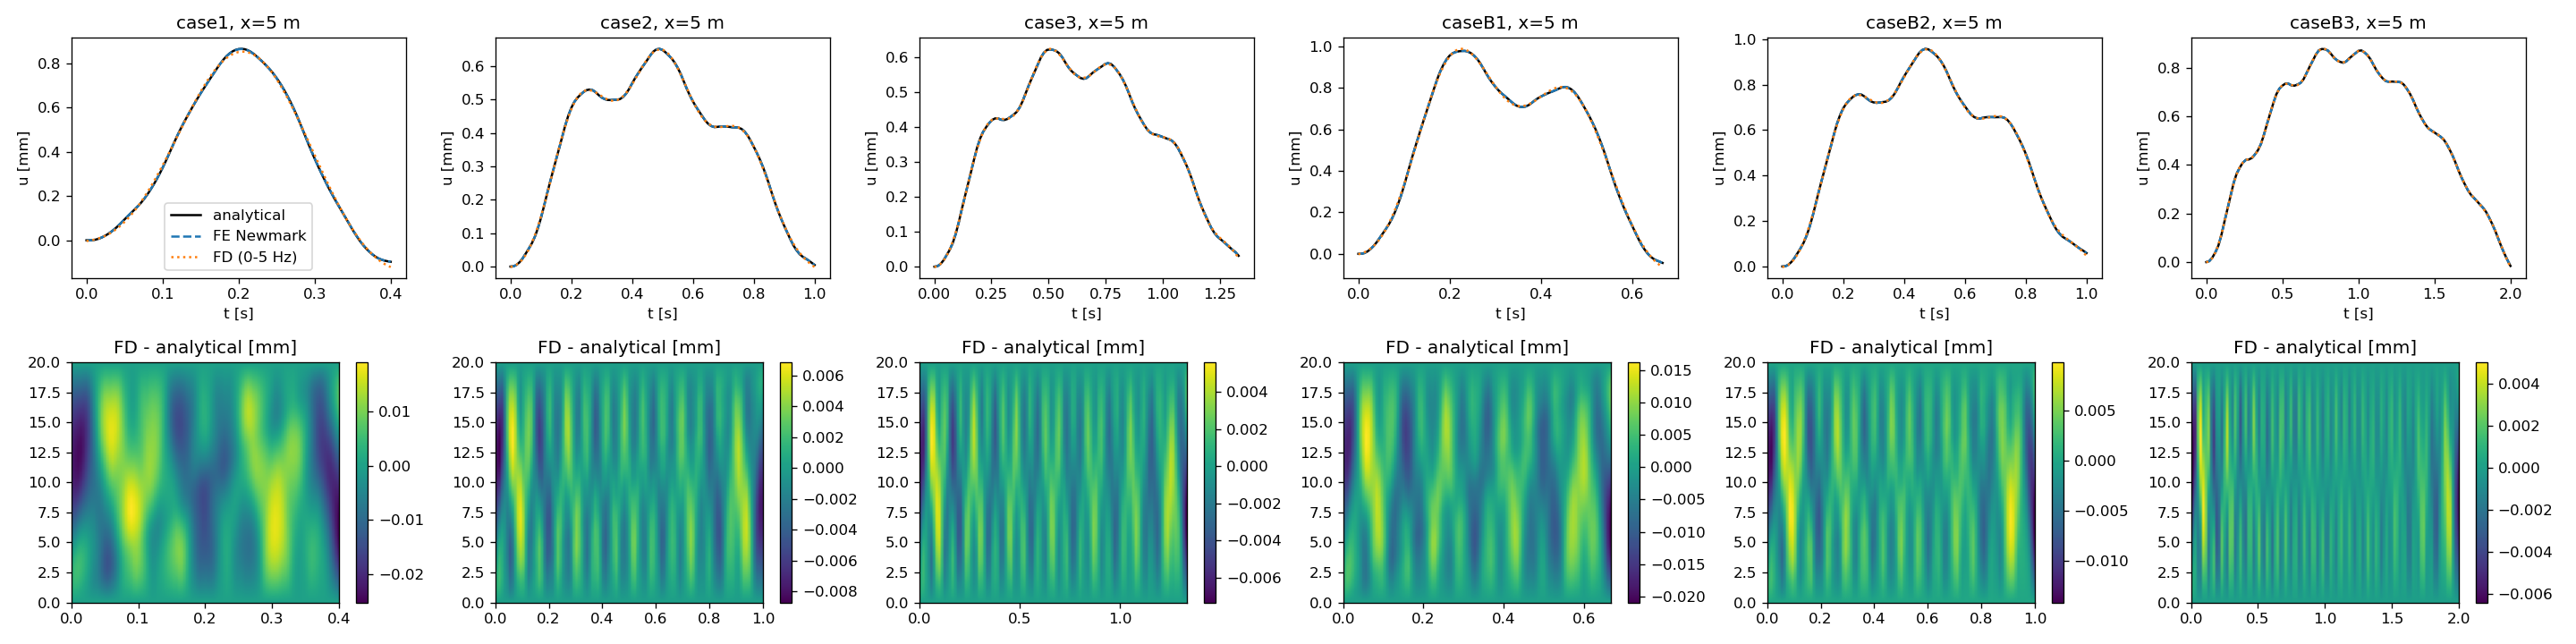
\includegraphics[width=0.9\linewidth]{figures/ch14r/fd_ref.png}
\caption{Reference solutions: analytical, finite element Newmark and the 0--5~Hz frequency-domain solution, and the band-limiting error field.}\label{fig:vf-fd-ref}
\end{figure}

\begin{table}[tbp]
\centering\footnotesize
\caption{Normalised mean-square error of the band-limited solution against the analytical one.}\label{tab:vf-fd-band}
\begin{tabular}{@{}rrrrrr@{}}
\toprule
Case & 2.5 Hz & 5 Hz (publication) & 10 Hz & 20 Hz & Publication's FD-PINN MSE\\
\midrule
1 & $1.2\times10^{-2}$ & $3.8\times10^{-5}$ & $1.0\times10^{-5}$ & $2.7\times10^{-7}$ & $4.7\times10^{-5}$\\
2 & $2.5\times10^{-3}$ & $5.6\times10^{-6}$ & $2.3\times10^{-6}$ & $5.8\times10^{-8}$ & $7.2\times10^{-5}$\\
3 & $1.2\times10^{-3}$ & $4.0\times10^{-6}$ & $1.4\times10^{-6}$ & $3.3\times10^{-8}$ & $7.0\times10^{-5}$\\
\bottomrule
\end{tabular}
\end{table}

\begin{figure}[tbp]
\centering
\includegraphics[width=0.9\linewidth]{figures/ch14_fdpinn.pdf}
\caption{Moving-load beam of \citet{liang2024fdpinn}. (a) Normalised error of the band-limited field against the band width, full-order sweep; the cost of the 5~Hz band is \cvfFdBandOne, \cvfFdBandTwo{} and \cvfFdBandThree{} for the three cases. (b) The same error from frequency-domain ROMs of size $r$; with ten modes they agree with the full-order value to within \cvfFdTen.}\label{fig:vf-fdpinn}
\end{figure}

For the comparison with the publication this matters as follows. In Case 1 the band alone accounts for $3.8\times10^{-5}$ of the publication's $4.7\times10^{-5}$ (about $80\,\%$), so its Case 1 result is close to the best any 0--5~Hz method can do; in Cases 2 and 3 the band accounts for only about $8\,\%$ and $6\,\%$ of its error, and the rest is network error, which is where this reproduction falls short.

\subsection*{Results: forward problem}

Only Case 3 was run forward. FD-PINN beats the time-domain PINN ($2.38\times10^{-3}$ against $3.90\times10^{-3}$) but not by the publication's margin: $7.0\times10^{-5}$ against $1.56\times10^{-3}$, a factor of 22, where this work obtains 1.6 (\Cref{tab:vf-fd-fwd}).

\begin{table}[tbp]
\centering\footnotesize
\caption{Forward problem, Case 3 (nMSE).}\label{tab:vf-fd-fwd}
\begin{tabular}{@{}lrrr@{}}
\toprule
Model & This work & Publication & Ratio\\
\midrule
Time-domain PINN & $3.90\times10^{-3}$ & $1.56\times10^{-3}$ & 2.5\\
FD-PINN & $2.38\times10^{-3}$ & $7.0\times10^{-5}$ & 34\\
\bottomrule
\end{tabular}
\end{table}

\emph{Time-domain PINN.} The plain recipe never left the near-zero solution; after the source Gaussian was widened and then narrowed during training, the best weights came at iteration 6000 when $\sigma/L$ had narrowed to about $0.019$. Without early stopping the error rose again to $0.027$. The result shows the spectral bias the publication describes: the network learns a smooth envelope and misses the 3.5~Hz oscillation (the double hump in the mid-span history), although the peak is close ($0.89$ against $0.87$~mm) (\Cref{fig:vf-fd-pinn}).

\emph{FD-PINN.} The nMSE stayed at $0.07$--$0.2$ for the first 7000 iterations, then fell to about $5\times10^{-3}$ at iteration 9000 and $2.4\times10^{-3}$ at 13\,000, where early stopping restored the weights. The error against the band-limited reference is $2.37\times10^{-3}$, so band truncation ($4\times10^{-6}$) is not the cause: the network under-fits the spectrum, reproducing the 0--1~Hz lobe but smoothing the small side lobes and the 3.5~Hz resonance peak, which is why the time history misses the double hump near $t=0.5$--$0.8$~s. The peak displacement is $0.869$ against $0.872$~mm (\Cref{fig:vf-fd-fdpinn}).

\begin{figure}[tbp]
\centering
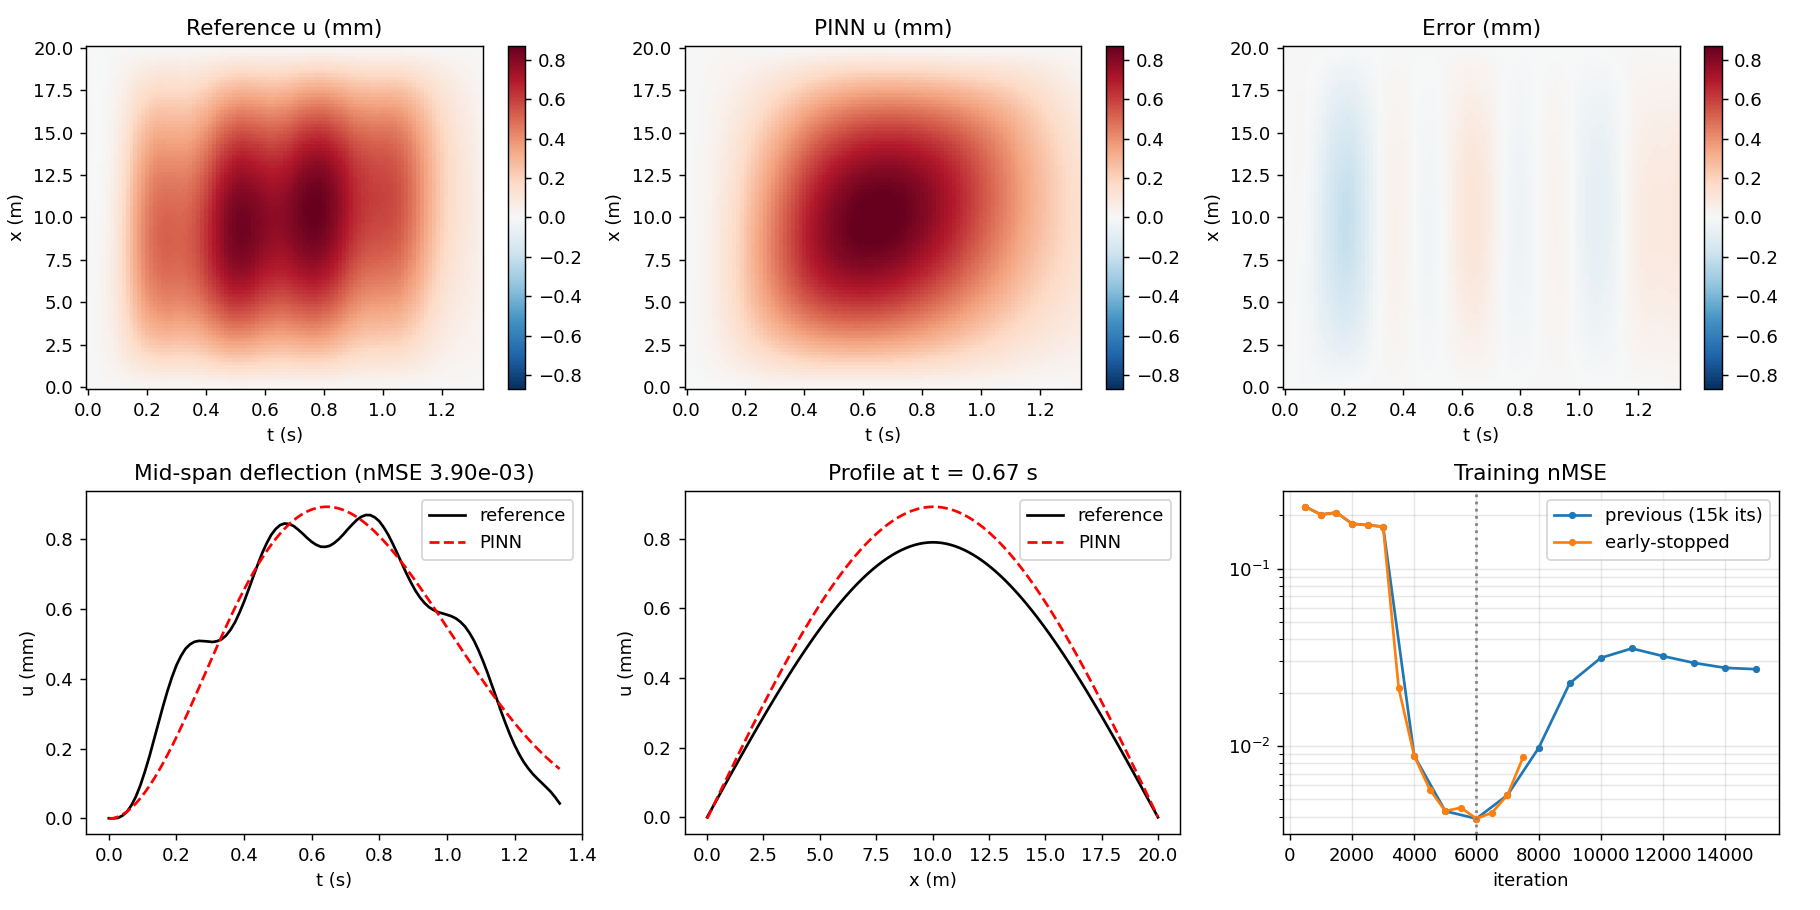
\includegraphics[width=0.95\linewidth]{figures/ch14r/fd_pinn.png}
\caption{Time-domain PINN, Case 3: fields, error, mid-span history, profile and training nMSE.}\label{fig:vf-fd-pinn}
\end{figure}

\begin{figure}[tbp]
\centering
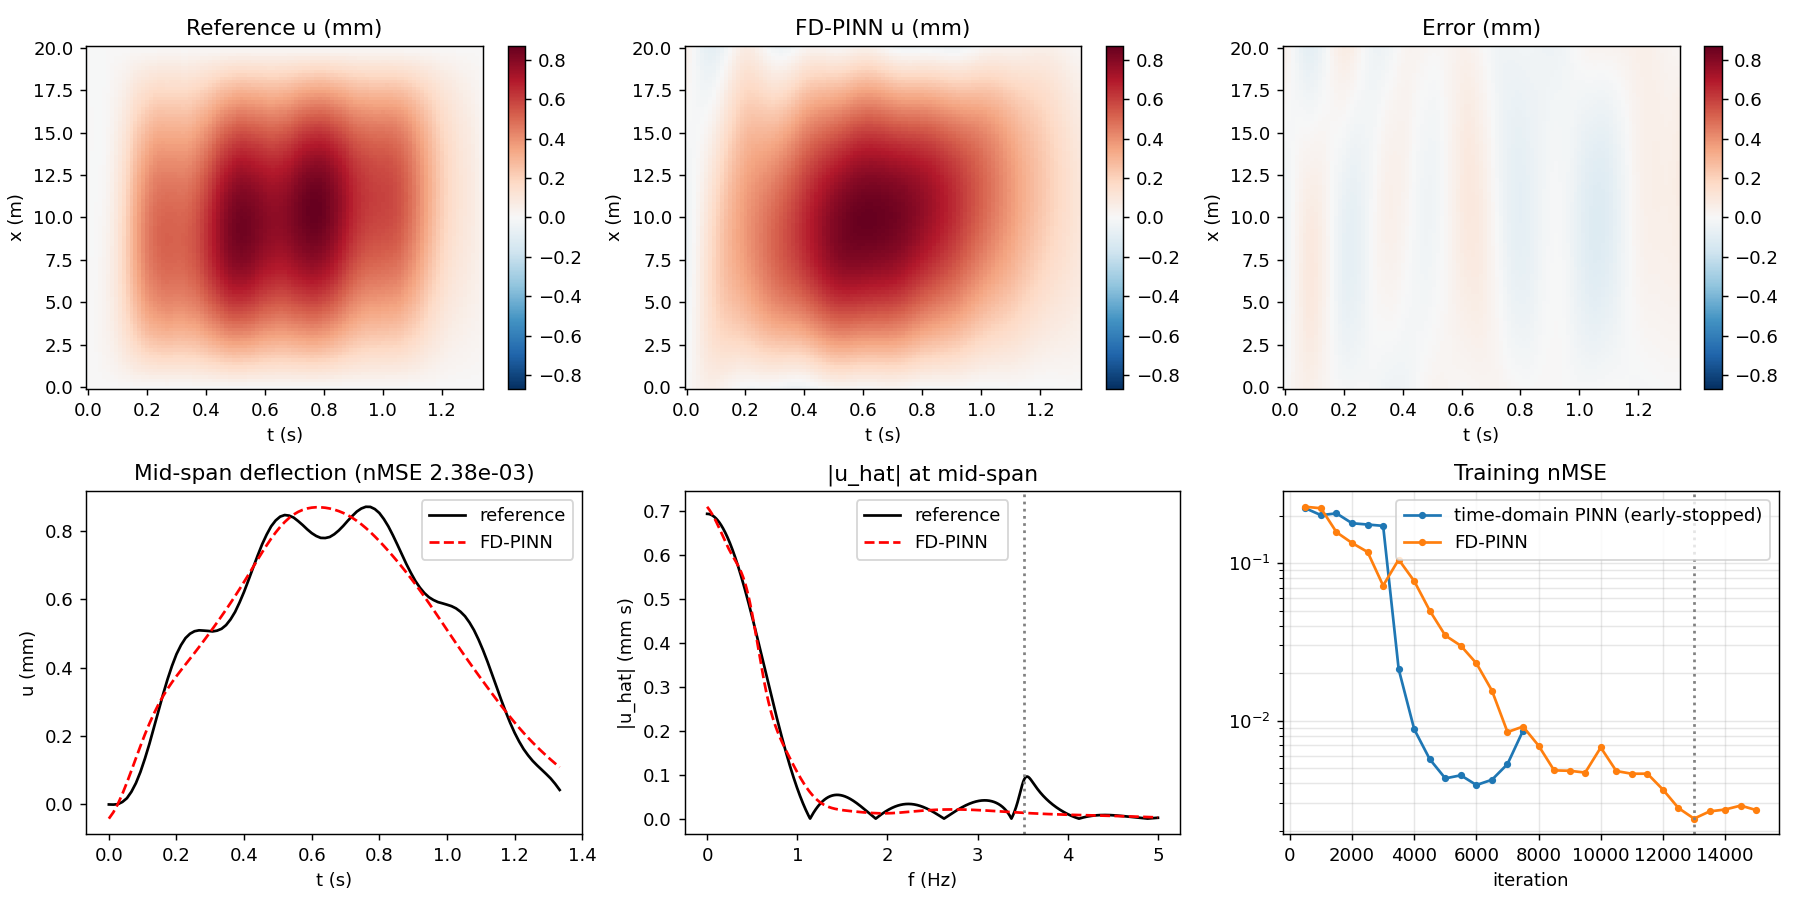
\includegraphics[width=0.95\linewidth]{figures/ch14r/fd_fdpinn.png}
\caption{FD-PINN, Case 3: fields, mid-span history, mid-span spectrum and training nMSE.}\label{fig:vf-fd-fdpinn}
\end{figure}

\emph{Attempts to close the gap.} \Cref{tab:vf-fd-try} lists three changes, none of which helped; the 20\,000-point run converged much faster early (nMSE $8.3\times10^{-3}$ at iteration 4500 against $5.0\times10^{-2}$) but plateaued, and a patience of four stopped it. The baseline had the same plateau before dropping at iteration 12\,000, so the comparison is inconclusive (\Cref{fig:vf-fd-cmp}).

\begin{table}[tbp]
\centering\footnotesize
\caption{Changes tried on the forward FD-PINN, Case 3.}\label{tab:vf-fd-try}
\begin{tabularx}{\linewidth}{@{}>{\raggedright\arraybackslash}p{5.2cm} >{\raggedright\arraybackslash}X >{\raggedright\arraybackslash}p{3.0cm}@{}}
\toprule
Change & Result & Outcome\\
\midrule
Frequency-normalised residual (divide by the mode-1 operator) & nMSE $0.24$ at iteration 3000 against $0.072$ baseline & worse; NaN restarts\\
Mode-1 amplitude envelope on the output & faster start, then stalled at $0.087$ & worse than baseline\\
20\,000 collocation points & $4.48\times10^{-3}$, stopped at iteration 8000 & not better; early stop may be premature\\
\bottomrule
\end{tabularx}
\end{table}

\begin{figure}[tbp]
\centering
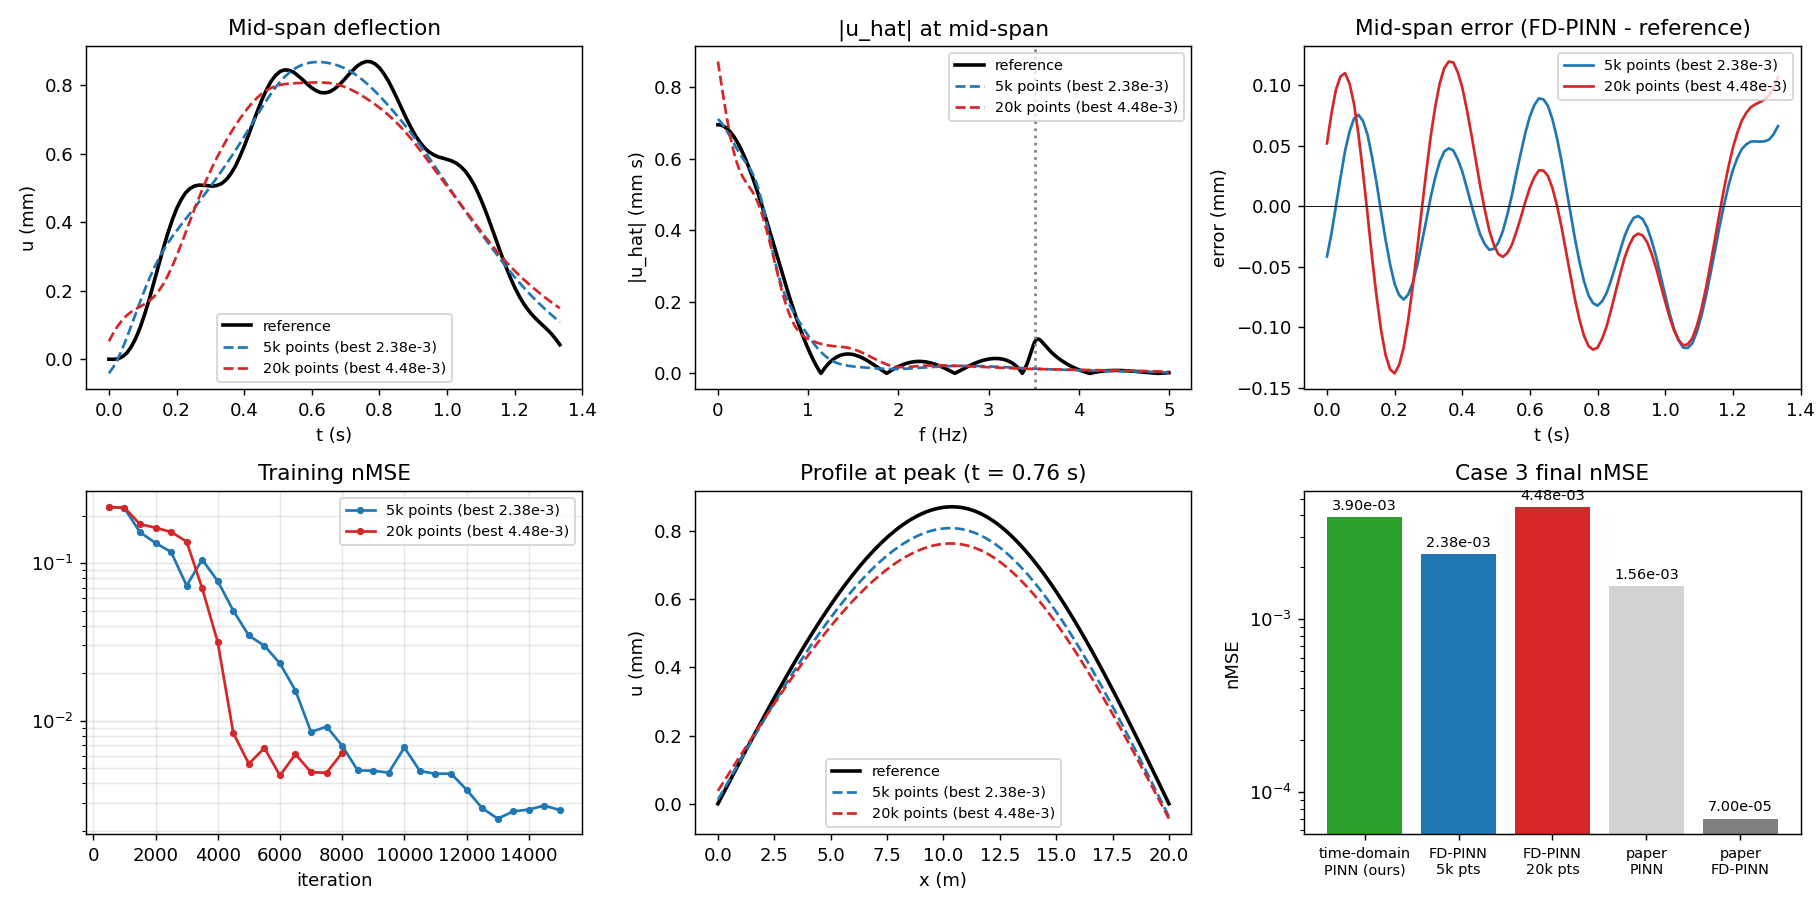
\includegraphics[width=0.95\linewidth]{figures/ch14r/fd_cmp.png}
\caption{FD-PINN with 5000 and 20\,000 collocation points: mid-span history, spectrum, profile and training nMSE.}\label{fig:vf-fd-cmp}
\end{figure}

\subsection*{Results: inverse problem}

At the publication's $10^4$-iteration budget the identification accuracy matches or exceeds the publication in all three cases (\Cref{tab:vf-fd-inv}), but its near $100\,\%$ at $4\times10^5$ iterations is not reached, and the field error is three times higher in Case 2 and fifteen times higher in Case 3 (Case 1 is below the publication's). The rule that picks the reported iteration matters: stopping on the true $EI$ is a benchmark-only shortcut that picked the moments when the $EI$ trace crossed $2.4\times10^9$ (Case 3 reached $97.6\,\%$ at iteration 5000, Case 2 $98.9\,\%$ at iteration 2000 with a field nMSE of $2.9\times10^{-3}$), which are not converged values; the loss-rule rows are the fair ones. For Case 1 the $EI$ sat within $0.1\,\%$ for thousands of iterations, so both rules agree.

\begin{table}[tbp]
\centering\footnotesize
\setlength{\tabcolsep}{4pt}
\caption{Inverse identification of $EI$.}\label{tab:vf-fd-inv}
\begin{tabular}{@{}lrrrrrr@{}}
\toprule
Case & $EI$ identified & Accuracy (this work) & Publication, $10^4$ its & Publication, $4\times10^5$ its & Field nMSE (this work) & Publication MSE\\
\midrule
1 (true-$EI$ rule) & $2.3999\times10^9$ & $100.0\,\%$ & $99.6\,\%$ & $100\,\%$ & $3.75\times10^{-5}$ & $4.72\times10^{-5}$\\
2 (loss rule) & $2.4264\times10^9$ & $98.9\,\%$ & $95.8\,\%$ & $100\,\%$ & $2.31\times10^{-4}$ & $7.15\times10^{-5}$\\
3 (loss rule) & $2.5382\times10^9$ & $94.6\,\%$ & $94.4\,\%$ & $100\,\%$ & $1.08\times10^{-3}$ & $7.01\times10^{-5}$\\
\bottomrule
\end{tabular}
\end{table}

Case 1 converges cleanly ($EI$ within $0.1\,\%$ from iteration 2000). Case 2 needed about 7500 iterations: $EI$ sat near $2.6\times10^9$ until iteration 4500 and then settled within $1$--$1.7\,\%$ of $2.4\times10^9$. Case 3 settles $5.7$--$6\,\%$ high from iteration 3000 while the loss keeps falling (\Cref{fig:vf-fd-train,fig:vf-fd-fields}). All runs use one seed, and the $5\,\%$-improvement stopping rule is weak: in both loss-rule runs many small drops of $2$--$3\,\%$ per evaluation kept resetting the patience counter, so the runs used the full 16\,000 iterations.

\begin{figure}[tbp]
\centering
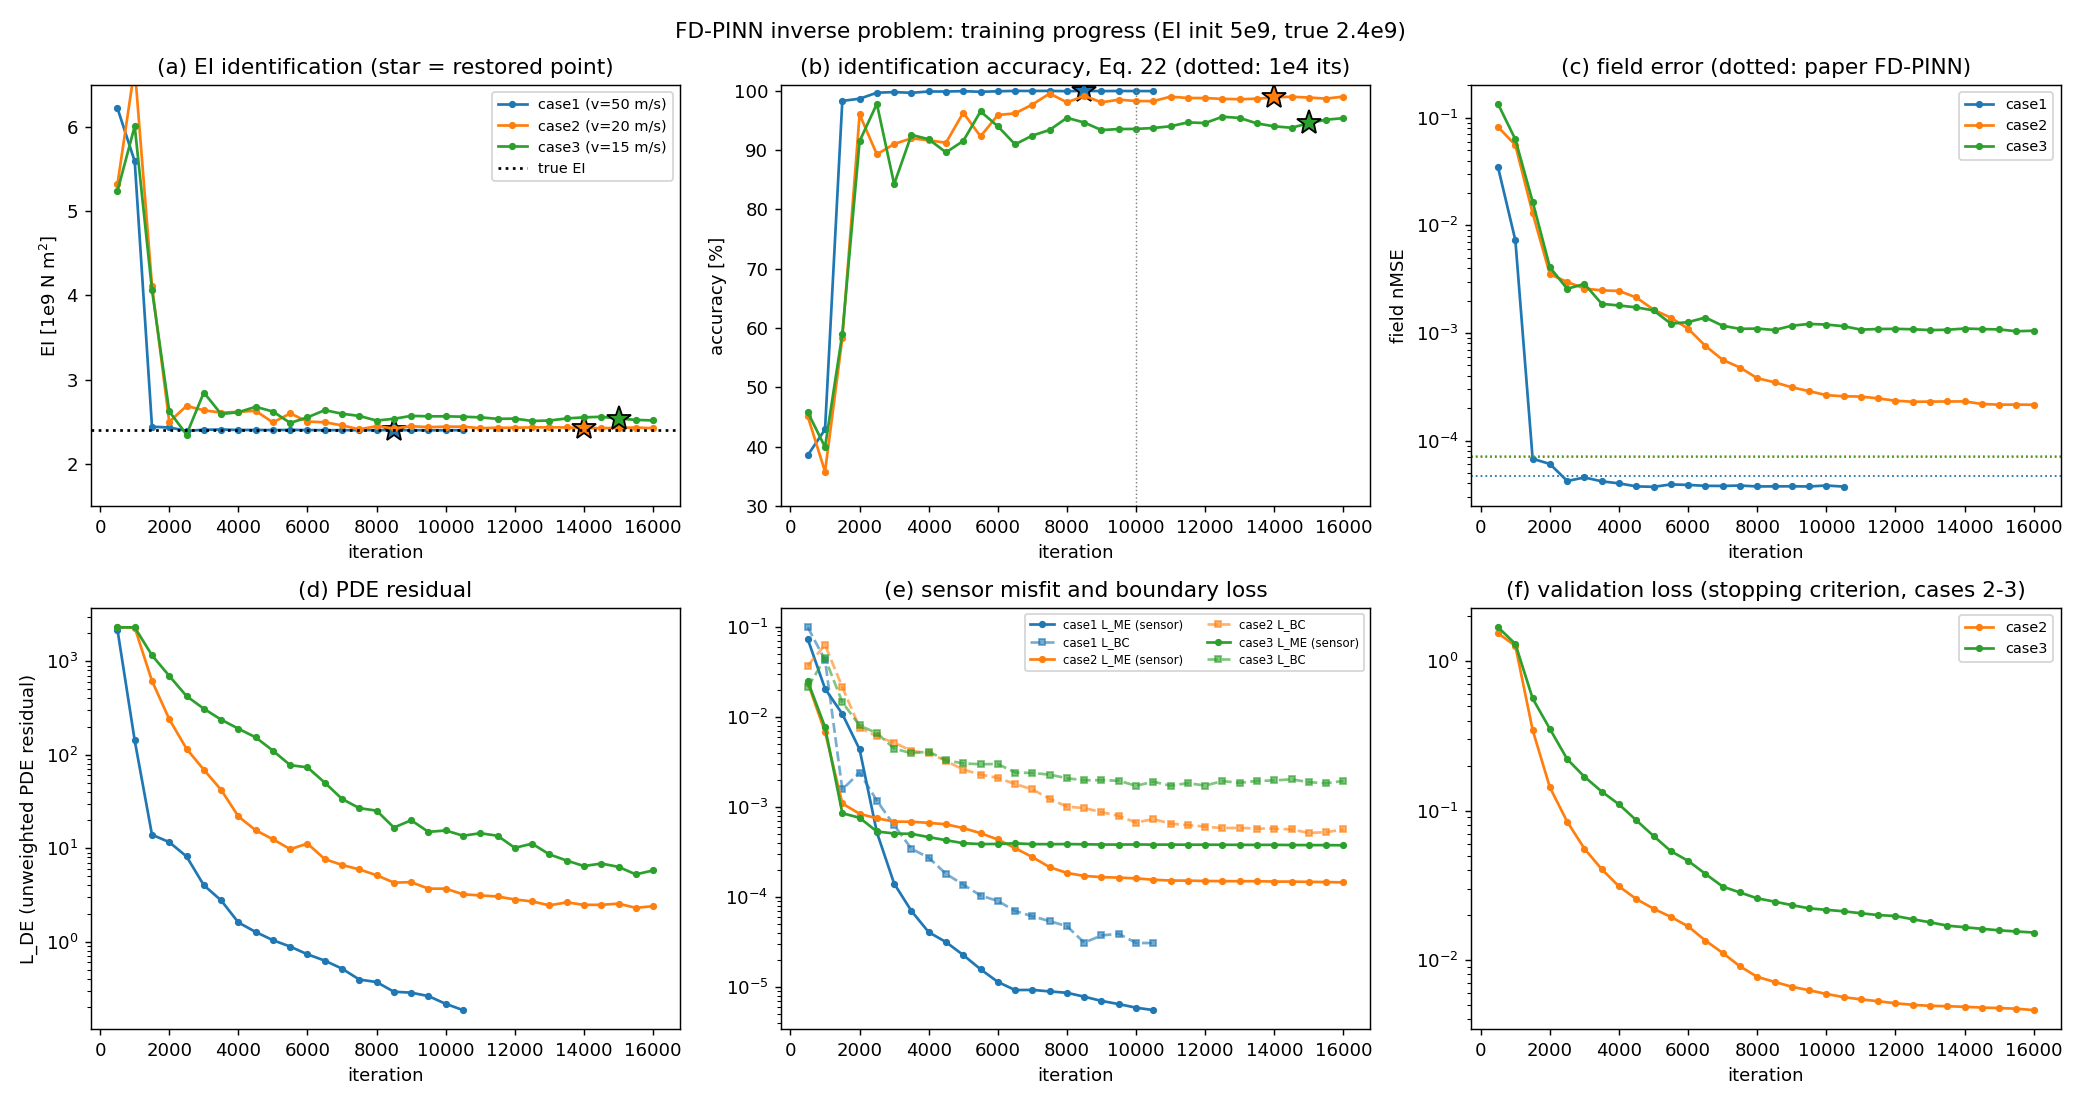
\includegraphics[width=0.95\linewidth]{figures/ch14r/fd_inv_train.png}
\caption{Inverse training: $EI$, accuracy and loss terms against iteration, three cases.}\label{fig:vf-fd-train}
\end{figure}

\begin{figure}[tbp]
\centering
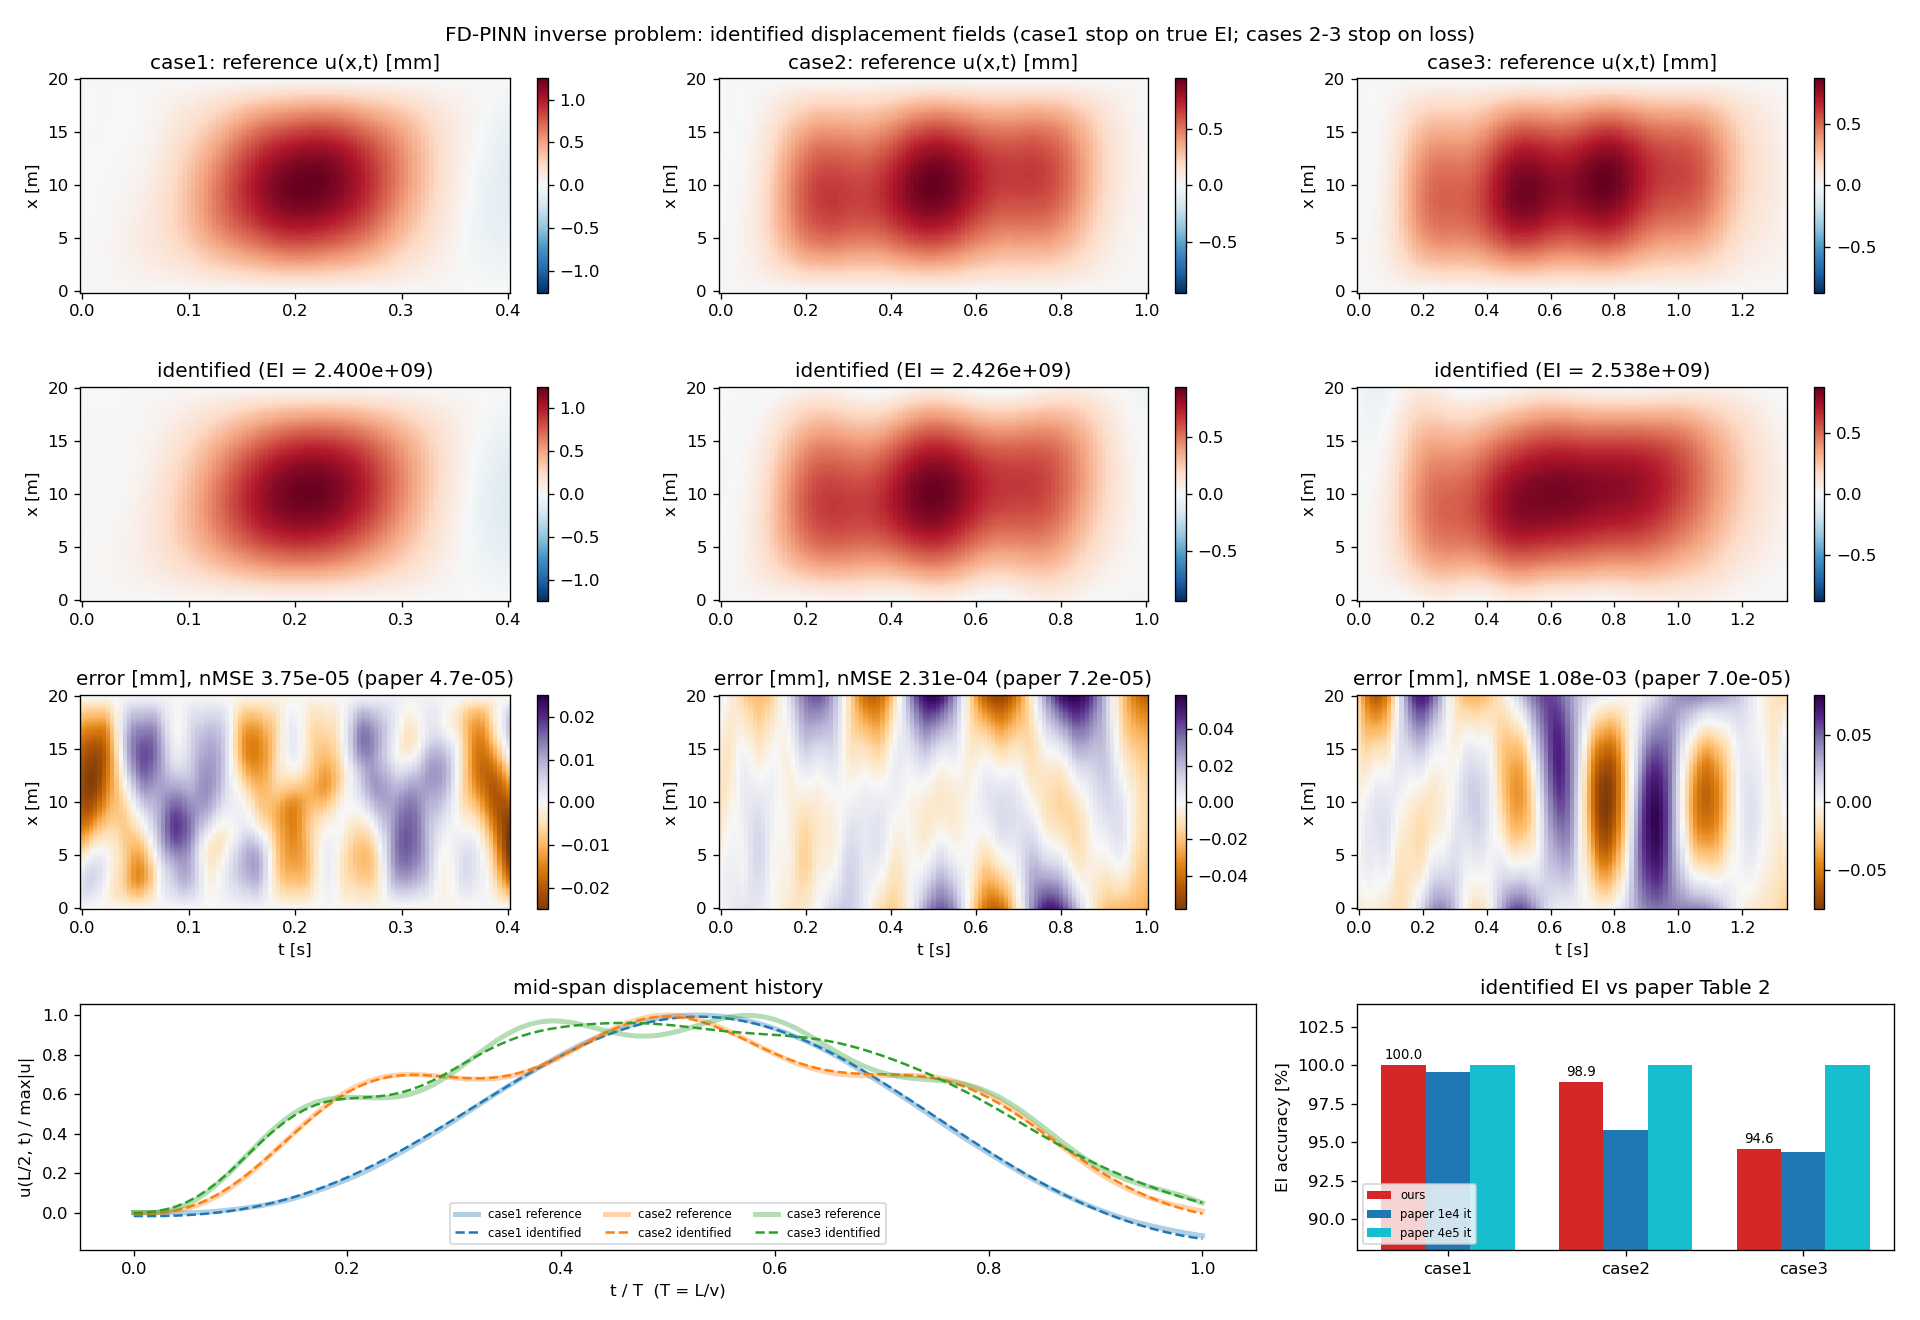
\includegraphics[width=0.95\linewidth]{figures/ch14r/fd_inv_fields.png}
\caption{Identified displacement fields, error maps, mid-span histories and accuracy against the publication, three cases.}\label{fig:vf-fd-fields}
\end{figure}

\emph{The Case 3 bias.} None of four changes removed the $+5.7$ to $+7.4\,\%$ error of $EI$ (\Cref{tab:vf-fd-bias}), so it is not caused by float precision, the number of sensor frequencies, the number of collocation points or a wider band at this budget. The 0--8~Hz run is worse because it is under-trained ($\mathcal L_{DE}$ stayed near 650 against about 7 at 5~Hz), so it is confounded with the budget and says nothing about band choice at a larger budget. The 20\,000-point run is the cleanest negative result: the same plateau at $2.65$--$2.70\times10^9$ (about $89\,\%$) until iteration 7500, then a drift to $2.51$--$2.55\times10^9$, with the accuracy wandering between $93.6\,\%$ and $95.6\,\%$ over the last 6000 iterations while the loss keeps falling; the restored point was iteration 15\,000 ($94.63\,\%$), and the last point ($95.59\,\%$) was not selected because picking it would need the true $EI$. A 61\,000-iteration run to test whether the bias is under-training was aborted at about iteration 5000 with $EI$ at $2.68\times10^9$ ($89.6\,\%$), before the point where the baseline leaves its plateau, so that hypothesis is neither confirmed nor ruled out.

\begin{table}[tbp]
\centering\footnotesize
\caption{Case 3 (loss rule): runs tried against the $EI$ bias.}\label{tab:vf-fd-bias}
\begin{tabular}{@{}lrrrr@{}}
\toprule
Run & $EI$ identified & Error & Accuracy & Field nMSE\\
\midrule
Baseline (5000 points, 201 frequencies, 0--5 Hz, fp32) & $2.5382\times10^9$ & $+5.8\,\%$ & $94.56\,\%$ & $1.08\times10^{-3}$\\
Full 16\,000 iterations, no early stop & $2.5506\times10^9$ & $+6.3\,\%$ & $94.10\,\%$ & not stored\\
float64 & $2.5778\times10^9$ & $+7.4\,\%$ & $93.10\,\%$ & $1.01\times10^{-3}$\\
801 sensor frequencies & $2.5561\times10^9$ & $+6.5\,\%$ & $93.89\,\%$ & $1.12\times10^{-3}$\\
20\,000 collocation points & $2.5361\times10^9$ & $+5.7\,\%$ & $94.63\,\%$ & $9.85\times10^{-4}$\\
0--8 Hz band & $2.8660\times10^9$ & $+19.4\,\%$ & $83.74\,\%$ & $3.45\times10^{-3}$\\
\bottomrule
\end{tabular}
\end{table}

\begin{figure}[tbp]
\centering
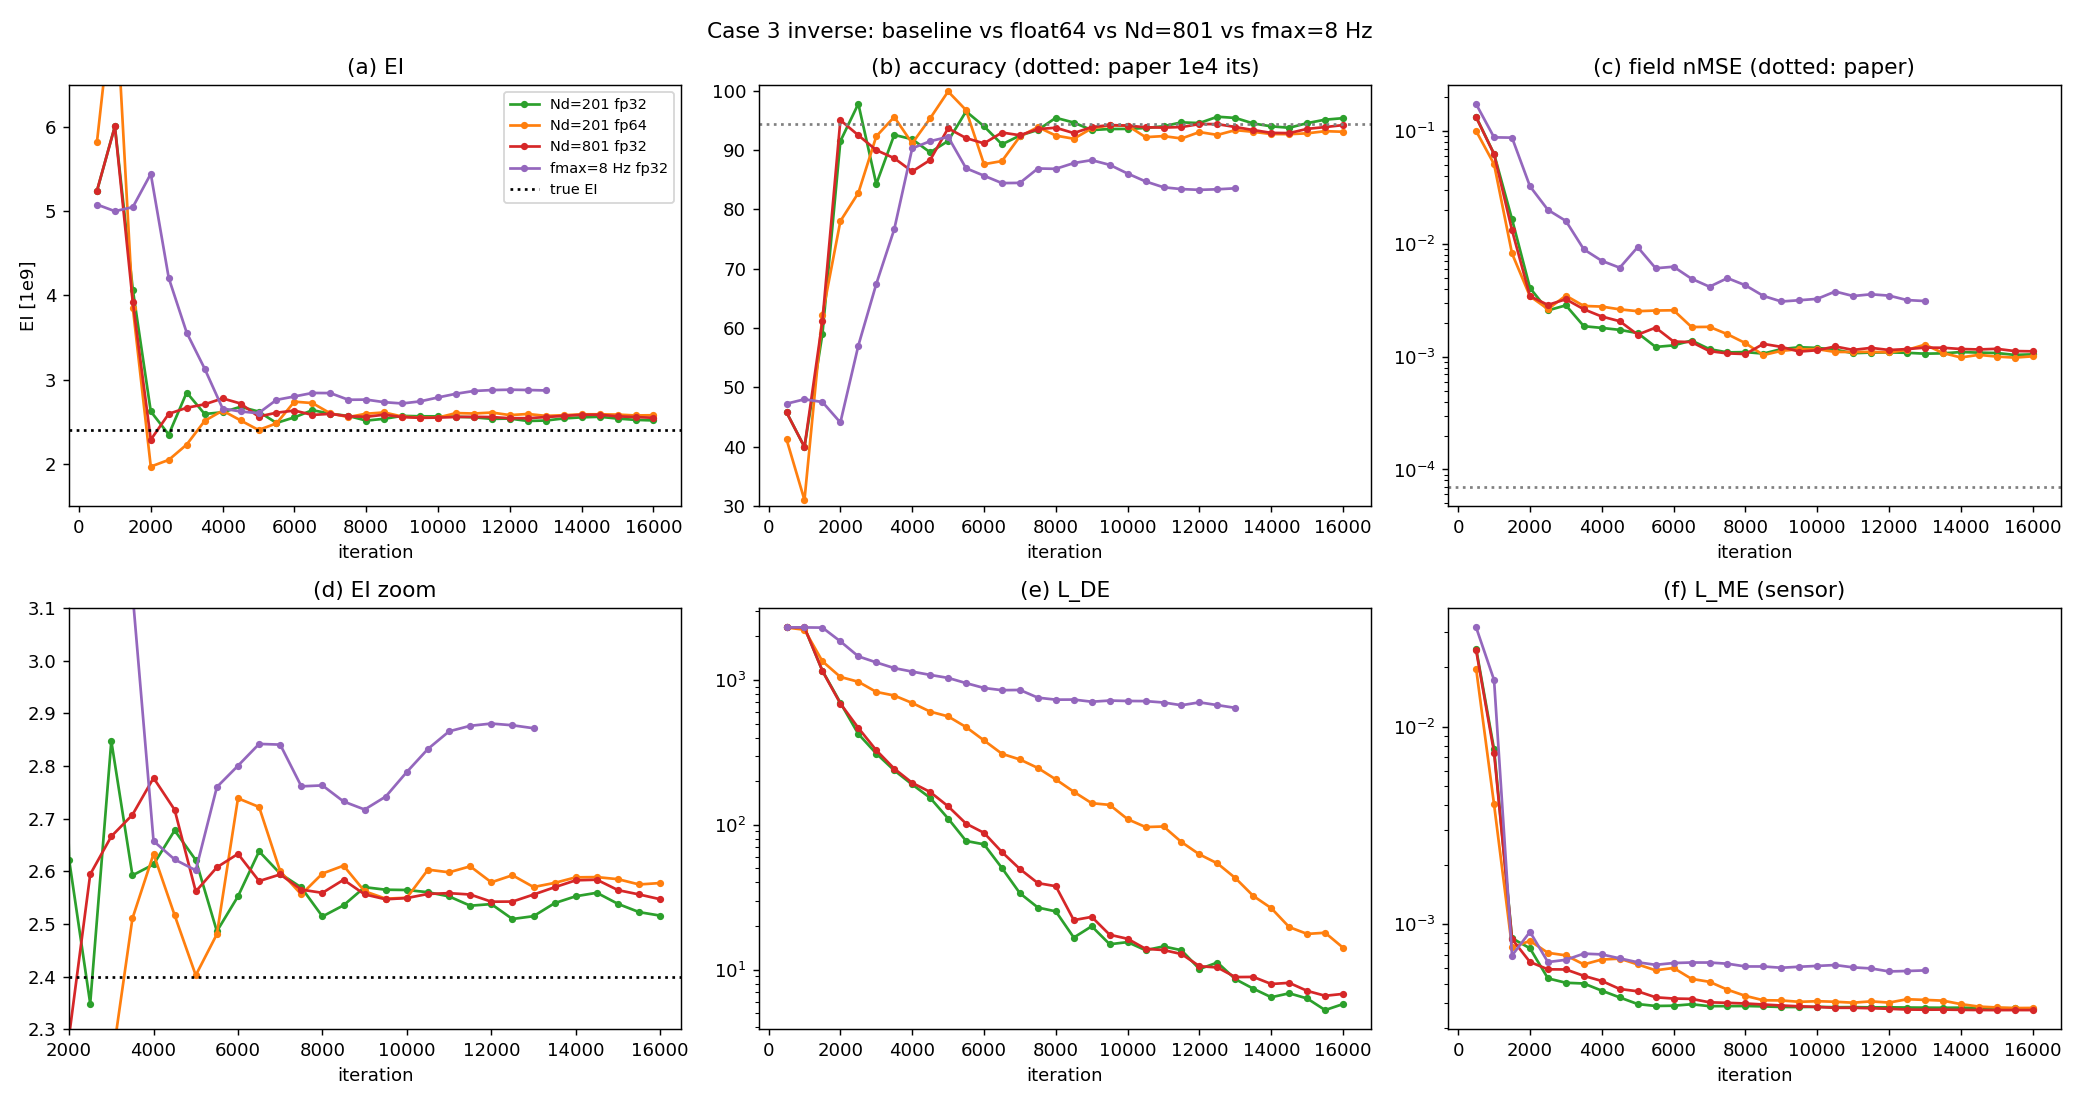
\includegraphics[width=0.95\linewidth]{figures/ch14r/fd_tests.png}
\caption{Case 3: $EI$, accuracy, nMSE and loss histories for the baseline, float64, 801-frequency and 0--8~Hz runs.}\label{fig:vf-fd-tests}
\end{figure}

\subsection*{Why the results differ from the publication}

The three mismatches share one most likely cause, a training budget about 30 times smaller than the publication's, but only one explanation is verified by calculation; \Cref{tab:vf-fd-why} labels the status of each.

\begin{table}[tbp]
\centering\footnotesize
\caption{Explanations of the mismatches and their status.}\label{tab:vf-fd-why}
\begin{tabularx}{\linewidth}{@{}>{\raggedright\arraybackslash}p{4.2cm} >{\raggedright\arraybackslash}X >{\raggedright\arraybackslash}p{3.0cm}@{}}
\toprule
Mismatch & Most likely explanation & Status\\
\midrule
Case 3 inverse field nMSE $1.08\times10^{-3}$ against $7\times10^{-5}$ & mostly the $EI$ bias, not a separate failure & verified by calculation\\
Case 3 $EI$ stays $+5.7\,\%$ high & under-training of a sharp, low-amplitude resonance feature & supported; one test aborted\\
Forward FD-PINN $2.4\times10^{-3}$ against $7\times10^{-5}$ & 30 times fewer iterations, 4 times fewer points, no output transform & supported by training curves, not isolated\\
Time-domain PINN needed a source-width ramp & unknown implementation difference & hypothesis\\
Ranking of Cases 2 and 3 & Case 3 carries the least resonance content & hypothesis, consistent with the publication\\
\bottomrule
\end{tabularx}
\end{table}

\emph{The field error is mostly the $EI$ bias (verified).} A field that solves the equation exactly with the wrong $EI$ is already far from the reference. Solving Case 3 analytically at the identified $EI$, with the damping held at its true value as in the inverse runs, gives an nMSE of $8.4\times10^{-4}$ at the 20\,000-point value of $EI$ and $8.6\times10^{-4}$ at the baseline's, which is $85\,\%$ and $80\,\%$ of the measured network errors ($9.85\times10^{-4}$ and $1.08\times10^{-3}$). A $5.7\,\%$ rise in $EI$ raises $f_1$ by $2.8\,\%$ (\cref{eq:fd-f1}), which shifts the resonance ripple out of phase with the reference. The field error of an exact solution grows roughly with the square of the $EI$ error, so the publication's inverse MSE of $7\times10^{-5}$ corresponds to an $EI$ error of about $1.6\,\%$ (accuracy near $98.4\,\%$); at $94.4\,\%$ the same calculation gives about $9\times10^{-4}$. The publication's inverse MSE most likely comes from a later, more accurate iterate than its $10^4$-iteration accuracy; the notes do not say which. The network does slightly better or worse than the exact solution at the same $EI$, and the exact solution at the biased $EI$ keeps the double hump while the network smooths it out, which is the spectral bias the publication describes (\Cref{fig:vf-fd-bias}).

\begin{figure}[tbp]
\centering
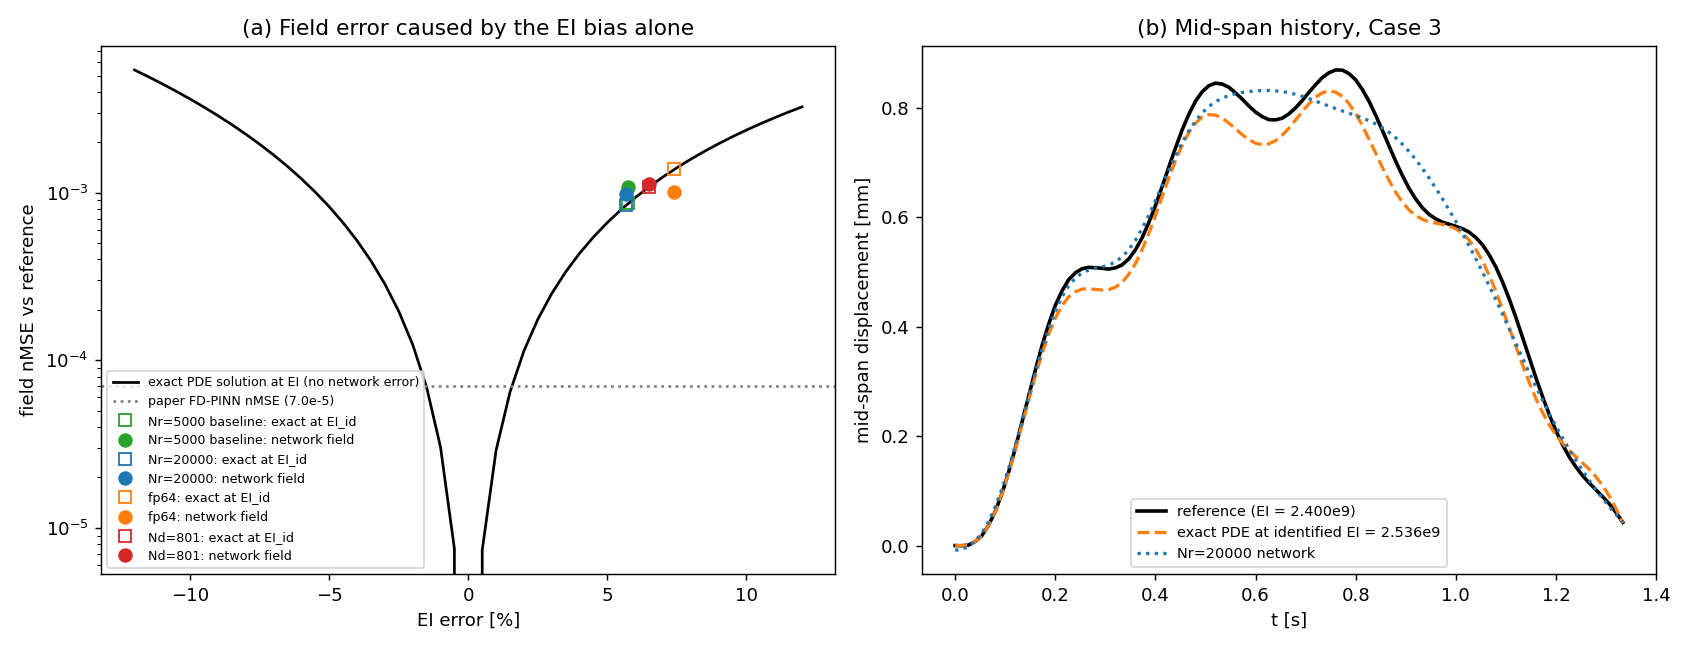
\includegraphics[width=0.95\linewidth]{figures/ch14r/fd_bias.png}
\caption{Left: field nMSE of an exact solution against the $EI$ error with the runs overlaid (squares: exact solution at the identified $EI$; circles: network field). Right: Case 3 mid-span history of the reference, the exact solution at the identified $EI$ and the network.}\label{fig:vf-fd-bias}
\end{figure}

\emph{Why Case 3 is the hardest (supported).} The load's own frequency is $v/2L$: $1.25$, $0.5$ and $0.375$~Hz, so $f_1$ is $2.8$, $7.0$ and $9.4$ times the load frequency. In Case 1 the beam is driven much closer to resonance and the response is mostly the large resonance term; in Case 3 it is mostly a quasi-static lobe with a small resonance ripple, which a $3\times60$ network must resolve along $\omega$ in a peak $3.5\,\%$ of the band wide while the rest of the spectrum is smooth. A network that cannot represent the ripple can absorb part of the misfit by moving $EI$, so both the residual and the sensor misfit are small at a biased $EI$: the loss keeps falling ($\mathcal L_{DE}$ from $2.3\times10^3$ to 4) but the misfit term is flat at about $3.7\times10^{-4}$. This is a hypothesis for the ordering and not a measured result; both the publication ($99.6$, $95.8$, $94.4\,\%$ at $10^4$ iterations) and this work ($100$, $98.9$, $94.6\,\%$) rank Case 1 first and Case 3 last.

\emph{Forward accuracy (supported).} The error against the band-limited reference is $2.37\times10^{-3}$, so the formulation and the band are not the limit ($4\times10^{-6}$); the residual loss was still falling after the restored iteration while the nMSE crept up, and the long plateau followed by sudden drops is typical of L-BFGS on a stiff PINN loss when the budget is short. The budget is 13\,000 iterations against $4\times10^5$, with 5000 collocation points against 20\,000 and no output transform; no single one was isolated. Single-precision L-BFGS (the NaN guard fired in several runs) and framework differences are plausible but unverified. For the time-domain PINN, the plain recipe is a known failure of PINNs with a narrow Gaussian source, because the zero solution has a small residual away from the load; the publication's code is stated as available only after publication, so initialisation, loss weights and the Dirac width cannot be compared, and the ratio of $2.5$ compares recipes as much as budgets.

\subsection*{Comparison with the publication}

\begin{table}[tbp]
\centering\footnotesize
\caption{Outcome of the reproduction of \citet{liang2024fdpinn}.}\label{tab:vf-fd-cmp}
\begin{tabularx}{\linewidth}{@{}>{\raggedright\arraybackslash}p{4.4cm} >{\raggedright\arraybackslash}X >{\raggedright\arraybackslash}p{2.6cm}@{}}
\toprule
Quantity & This work & Outcome\\
\midrule
Reference solutions & analytical, Newmark, modal agree to $\sim10^{-7}$; band cost $3.8\times10^{-5}$, $5.6\times10^{-6}$, $4.0\times10^{-6}$ & reproduced\\
Inverse accuracy, Cases 1--3 & $100.0$, $98.9$, $94.6\,\%$ against $99.6$, $95.8$, $94.4\,\%$ & reproduced at $10^4$ its\\
Inverse near-$100\,\%$ at $4\times10^5$ iterations & not run & not tested\\
Forward FD-PINN, Case 3 & $2.38\times10^{-3}$ against $7.0\times10^{-5}$ & not reproduced (34$\times$)\\
Time-domain PINN, Case 3 & $3.90\times10^{-3}$ against $1.56\times10^{-3}$ (with a source ramp) & not reproduced (2.5$\times$)\\
Inverse-run field error, Case 3 & $1.08\times10^{-3}$ against about $7\times10^{-5}$ & not reproduced (about 15$\times$)\\
\bottomrule
\end{tabularx}
\end{table}

\subsection*{What remains unchecked}

Five parts of the publication remain unchecked. The appendix beams B1--B3 have reference solutions, but FD-PINN has not been run on them. Only Case 3 was run forward. The long-budget test that would show whether the $EI$ bias disappears with training was aborted. At least three seeds per result are needed before differences of one or two accuracy points mean anything, because within one run the Case 3 accuracy moved between $93.6\,\%$ and $95.6\,\%$ over the last 6000 iterations; only the $19.4\,\%$ error of the 0--8~Hz run and the $5$--$7\,\%$ bias common to all runs exceed that spread. And noisy sensor data were not used, where the publication's inverse tests may include noise. The resonance hypothesis could be tested without further training by comparing the sensitivity of the sensor misfit to $EI$ in Cases 1 and 3.

\section{A neural operator informed by a ROM}\label{sec:vf-frino}

\subsection*{Concept and purpose}

\citet{yang2025frino} train a Fourier neural operator (FNO) to map an excitation history to the structural response, and add to the data loss a term that penalises the residual of a low-order POD Galerkin ROM of the same structure. The ROM supplies the physics at the cost of a few reduced equations, the finite element model supplies the training labels, and the trained operator is meant to predict responses to new waveforms in milliseconds. The study rebuilds the pipeline end to end (a three-dimensional finite element cantilever, its POD ROM, the operator, the publication's test loads and parameter studies) and adds checks the publication omits: whether the operator is linear, how much the physics term contributes, how strong a tuned PINN baseline is, and what the exact frequency-domain solution of this linear problem costs.

The packages supply the finite element model (\anchor{fea_engine.elements.Hex20}), the POD ROM and the Newmark integrators of \rom{}, the exact frequency-domain solve (paper Eq.~20) and, for double precision, the FNO blocks of \rom{}; the network training itself used PyTorch on a 3~GB GPU in single precision.

\subsection*{Mathematics as implemented}

The full-order model is $\mathbf M\ddot{\mathbf u}+\mathbf C\dot{\mathbf u}+\mathbf K\mathbf u=\mathbf f\,g(t)$ with Rayleigh damping $\mathbf C=0.154\,\mathbf M+0.00078\,\mathbf K$. A POD basis $\boldsymbol\Psi$ of three modes is built from 200 snapshots of the single-tone responses, $\mathbf u\approx\boldsymbol\Psi\mathbf q$, giving the ROM
\begin{equation}\label{eq:fr-rom}
\mathbf M_r\ddot{\mathbf q}+\mathbf C_r\dot{\mathbf q}+\mathbf K_r\mathbf q=\boldsymbol\Psi^{T}\mathbf f\,g(t).
\end{equation}
The operator maps the excitation $g$ on the time grid to the reduced coordinates $\mathbf q$, and is trained on
\begin{equation}\label{eq:fr-loss}
\mathcal L=\mathcal L_{\rm data}+\lambda\,\mathcal L_{\rm ROM},\qquad
\mathcal L_{\rm ROM}=\big\lVert\mathbf M_r\ddot{\mathbf q}_\theta+\mathbf C_r\dot{\mathbf q}_\theta+\mathbf K_r\mathbf q_\theta-\boldsymbol\Psi^{T}\mathbf f\,g\big\rVert^2,
\end{equation}
with the time derivatives of the network output formed by finite differences on the time grid; the data loss is on the labels of the ROM time stepping at the training points. All errors are relative $L_2$ against the 4239-degree-of-freedom response unless stated, evaluated through the projection identity
\begin{equation}\label{eq:fr-err}
\lVert\mathbf u-\boldsymbol\Psi\mathbf q\rVert^2=\lVert\mathbf u\rVert^2-2\langle\boldsymbol\Psi^{T}\mathbf u,\mathbf q\rangle+\lVert\mathbf q\rVert^2,
\end{equation}
which gives full-field errors without storing the full-order fields. Because the ROM is linear and time-invariant, its response to a harmonic load follows from a frequency-domain solve of \cref{eq:fr-rom} (the publication's Eq.~20), exact up to the discretisation of the transform; this is the baseline against which the operator's cost is compared. A forced--transient split of the ROM response is used to interpret the high-frequency errors.

\subsection*{Geometry and mesh}

The structure is the cantilever of the publication, $60\times15\times1.5$~mm, with a point load at the midpoint of the free end, transverse to the thickness (\Cref{fig:vf-fr-geom}). The publication used an ANSYS Solid186 model with 4239 degrees of freedom; the analogue here is a $14\times8\times2$ mesh of twenty-node hexahedra, with 1413 nodes, 4239 degrees of freedom and 4032 free ones. Material constants are printed in a garbled unit string in the publication; they are used as printed ($E=2\times10^5$~N/mm$^2$, $\rho=7.9\times10^{-6}$), which gives $f_1=10.9$~Hz against the publication's 10~Hz, and the consistent-unit alternative gives 345~Hz. \Cref{tab:vf-fr-setup} lists what the publication states and what was chosen.

\begin{figure}[tbp]
\centering
\includegraphics[width=0.9\linewidth]{figures/ch14_geom_frino.pdf}
\caption{Cantilever of the neural-operator study, drawn from the data of the report: $14\times8\times2$ Hex20 elements, clamped end and the transverse point load at the free end.}\label{fig:vf-fr-geom}
\end{figure}

\begin{table}[tbp]
\centering\footnotesize
\caption{Set-up of the neural-operator study.}\label{tab:vf-fr-setup}
\begin{tabularx}{\linewidth}{@{}>{\raggedright\arraybackslash}p{2.6cm} >{\raggedright\arraybackslash}X >{\raggedright\arraybackslash}X@{}}
\toprule
Item & Publication & This work\\
\midrule
Geometry & $60\times15\times1.5$ mm cantilever, point load at free-end midpoint & same; load transverse to the thickness\\
Model & ANSYS Solid186, 4239 dofs & \texttt{Hex20}, $14\times8\times2$, 4239 dofs (4032 free)\\
Material & $E$, $\rho$ in a garbled unit string & $E=2\times10^5$ N/mm$^2$, $\rho=7.9\times10^{-6}$ as printed ($f_1=10.9$ Hz)\\
Damping & $\mathbf C=0.154\,\mathbf M+0.00078\,\mathbf K$ & same\\
Time window & 0.41 s, 8192 points, 6.25\,\% (512 points) for training & same\\
POD & 200 snapshots, 3 modes & 200 snapshots from the 8 single-tone responses (which response is not stated), 3 modes\\
FNO & 4 Fourier layers, width 256 & same; 64 Fourier modes (not stated); time-grid channel appended\\
Training & 500 epochs, batch 20, Adam lr $10^{-3}$, $\times0.4$ every 100 epochs, $\lambda=10^{-3}$ & same; weight decay $10^{-4}$\\
Training set & not stated & 8 paper tones + 32 random single tones in 2--120 Hz (40)\\
Loss scaling & raw & data loss on normalised modes; ROM residual normalised by the mean-square reduced load\\
Equations 35--36 & ``501 Hz'', ``701 Hz'' & read as 50 Hz, 70 Hz\\
Precision & --- & single (double supported with \rom{}'s own FNO blocks)\\
\bottomrule
\end{tabularx}
\end{table}

\subsection*{Results: full-order model, POD and ROM}

The first natural frequencies of the model are $10.9$, $68.2$, $85.0$, $102.9$ and $191.2$~Hz. The POD cumulative energy is $99.9871$, $99.99970$ and $100.00000\,\%$ for one, two and three modes against $94.610$, $99.954$ and $99.999\,\%$ in the publication, a difference that follows from the snapshot source, which the publication does not state. The three-mode ROM has eigenfrequencies $10.9$, $68.2$ and $227.8$~Hz and Rayleigh damping ratios $0.028$, $0.167$ and $0.558$. Solver cross-checks agree: GPU batched Newmark against CPU SuperLU Newmark on the tip degree of freedom to $5.9\times10^{-9}$, the study's beam integrator against \fea{}'s implicit transient to $10^{-9}$ (a unit test), and the GPU stiffness assembly against the loop assembly to $4\times10^{-15}$. \Cref{tab:vf-fr-ref} and \Cref{fig:vf-fr-fom} give the validation per load.

\begin{table}[tbp]
\centering\footnotesize
\caption{Reference-solver validation (three-mode ROM).}\label{tab:vf-fr-ref}
\begin{tabular}{@{}lrrr@{}}
\toprule
Load & POD truncation & 3-mode ROM against FEM & Eq.~(20) FFT solve against ROM stepping\\
\midrule
5 Hz & $4.924\times10^{-5}$ & $7.350\times10^{-5}$ & $3.781\times10^{-6}$\\
10 Hz & $1.016\times10^{-5}$ & $1.519\times10^{-5}$ & $1.224\times10^{-5}$\\
15 Hz & $4.653\times10^{-5}$ & $6.949\times10^{-5}$ & $8.112\times10^{-6}$\\
20 Hz & $9.246\times10^{-5}$ & $1.382\times10^{-4}$ & $9.140\times10^{-6}$\\
95 Hz & $1.466\times10^{-3}$ & $2.425\times10^{-3}$ & $8.301\times10^{-5}$\\
100 Hz & $1.738\times10^{-3}$ & $2.891\times10^{-3}$ & $7.795\times10^{-5}$\\
105 Hz & $2.085\times10^{-3}$ & $3.493\times10^{-3}$ & $7.448\times10^{-5}$\\
110 Hz & $2.499\times10^{-3}$ & $4.219\times10^{-3}$ & $7.213\times10^{-5}$\\
Fm1 & $1.977\times10^{-4}$ & $3.168\times10^{-4}$ & $1.774\times10^{-5}$\\
Fm2 & $6.252\times10^{-4}$ & $1.084\times10^{-3}$ & $4.036\times10^{-5}$\\
Fr1 & $1.745\times10^{-4}$ & $2.833\times10^{-4}$ & $1.732\times10^{-5}$\\
Fr2 & $1.374\times10^{-4}$ & $2.234\times10^{-4}$ & $1.743\times10^{-5}$\\
\bottomrule
\end{tabular}
\end{table}

\begin{figure}[tbp]
\centering
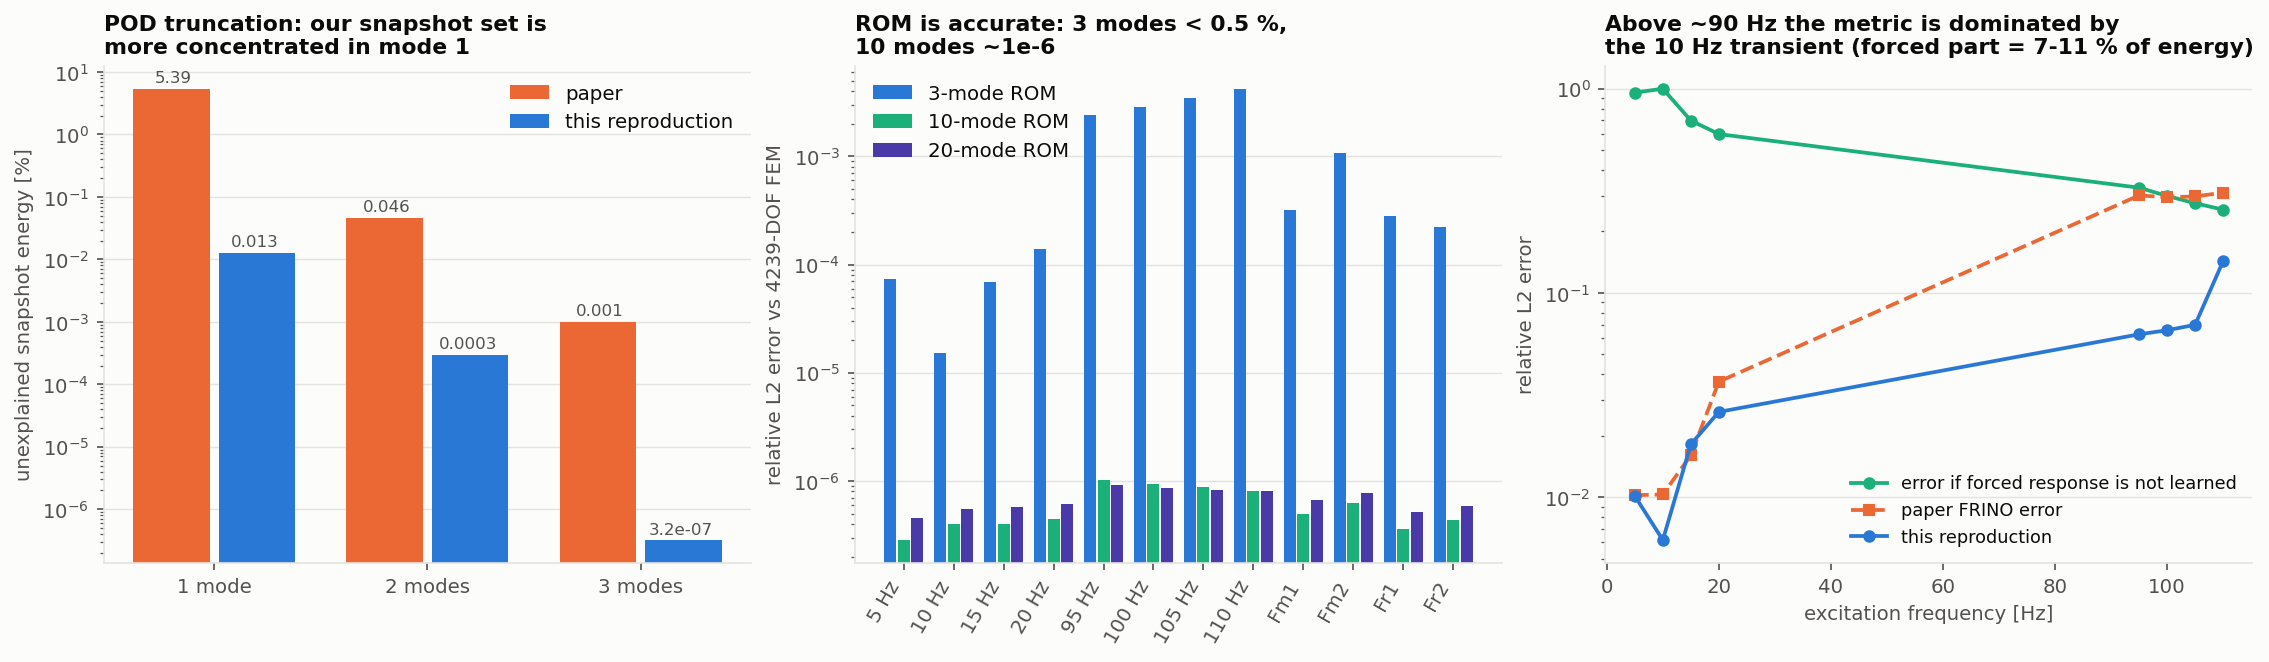
\includegraphics[width=0.98\linewidth]{figures/ch14r/fr_fom.png}
\caption{(a) Unexplained snapshot energy after 1--3 POD modes, publication against this work. (b) Relative error of the 3-, 10- and 20-mode ROM against the 4239-dof model for all 12 loads. (c) Error floor if the forced response is not learned, against the publication's and this work's single-tone errors.}\label{fig:vf-fr-fom}
\end{figure}

\subsection*{Results: the operator on the publication's loads}

The default run has 33.9 million parameters, trains in 139~s and is evaluated on all 12 loads (eight single tones at 5, 10, 15, 20, 95, 100, 105 and 110~Hz, two multi-frequency loads Fm1, Fm2 and two random loads Fr1, Fr2). \Cref{tab:vf-fr-err} and \Cref{fig:vf-fr-err} compare with the publication. Single tones reproduce, with a mean of $1.5\times10^{-2}$ at 5--20~Hz (publication $1.8\times10^{-2}$) and $8.5\times10^{-2}$ at 95--110~Hz (publication $0.3$); the multi-frequency and random loads do not. The errors on the training grid and on a grid sixteen times finer agree to within a factor of two, and the errors against the ROM labels and against the finite element model agree to three digits, so POD truncation is not what limits accuracy.

\begin{table}[tbp]
\centering\footnotesize
\caption{Relative $L_2$ error against the 4239-dof FEM.}\label{tab:vf-fr-err}
\begin{tabular}{@{}lrrrr@{}}
\toprule
Load & Publication & This work, training grid & This work, 16$\times$ finer grid & Against ROM (finer grid)\\
\midrule
5 Hz & $1.02\times10^{-2}$ & $9.46\times10^{-3}$ & $1.01\times10^{-2}$ & $1.01\times10^{-2}$\\
10 Hz & $1.03\times10^{-2}$ & $4.76\times10^{-3}$ & $6.17\times10^{-3}$ & $6.17\times10^{-3}$\\
15 Hz & $1.60\times10^{-2}$ & $1.70\times10^{-2}$ & $1.81\times10^{-2}$ & $1.81\times10^{-2}$\\
20 Hz & $3.68\times10^{-2}$ & $2.61\times10^{-2}$ & $2.62\times10^{-2}$ & $2.62\times10^{-2}$\\
95 Hz & $3.00\times10^{-1}$ & $6.38\times10^{-2}$ & $6.27\times10^{-2}$ & $6.27\times10^{-2}$\\
100 Hz & $2.94\times10^{-1}$ & $6.95\times10^{-2}$ & $6.57\times10^{-2}$ & $6.56\times10^{-2}$\\
105 Hz & $2.97\times10^{-1}$ & $7.67\times10^{-2}$ & $6.98\times10^{-2}$ & $6.97\times10^{-2}$\\
110 Hz & $3.10\times10^{-1}$ & $9.92\times10^{-2}$ & $1.43\times10^{-1}$ & $1.43\times10^{-1}$\\
Fm1 & $1.29\times10^{-1}$ & $4.12\times10^{-1}$ & $4.07\times10^{-1}$ & $4.07\times10^{-1}$\\
Fm2 & $2.02\times10^{-1}$ & $5.36\times10^{-1}$ & $4.80\times10^{-1}$ & $4.80\times10^{-1}$\\
Fr1 & $9.65\times10^{-2}$ & $7.74\times10^{-1}$ & $7.74\times10^{-1}$ & $7.74\times10^{-1}$\\
Fr2 & $9.87\times10^{-2}$ & $6.09\times10^{-1}$ & $6.08\times10^{-1}$ & $6.08\times10^{-1}$\\
\bottomrule
\end{tabular}
\end{table}

\begin{figure}[tbp]
\centering
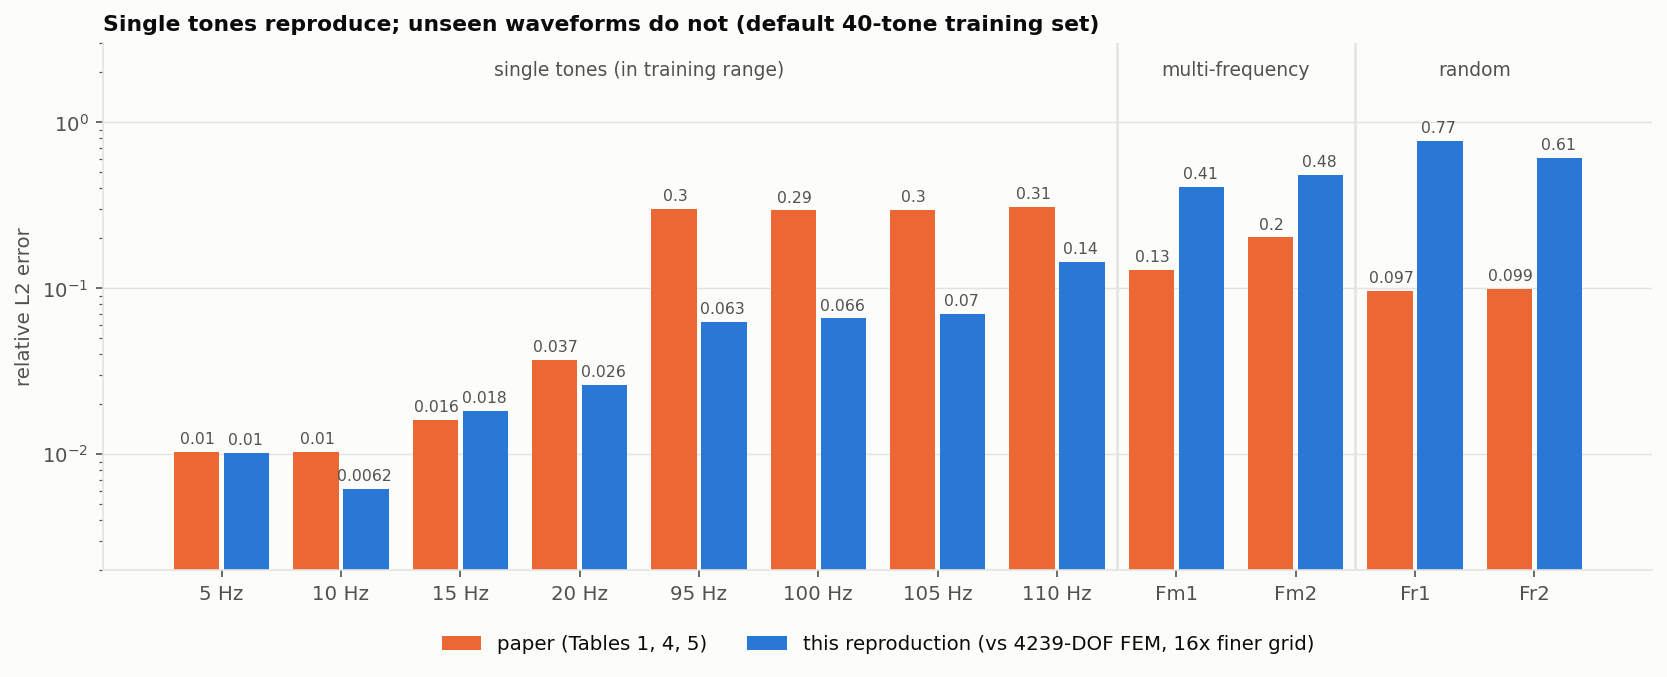
\includegraphics[width=0.9\linewidth]{figures/ch14r/fr_err.png}
\caption{Relative $L_2$ error for the 12 test loads: publication (Tables 1, 4, 5) against this work.}\label{fig:vf-fr-err}
\end{figure}

\begin{figure}[tbp]
\centering
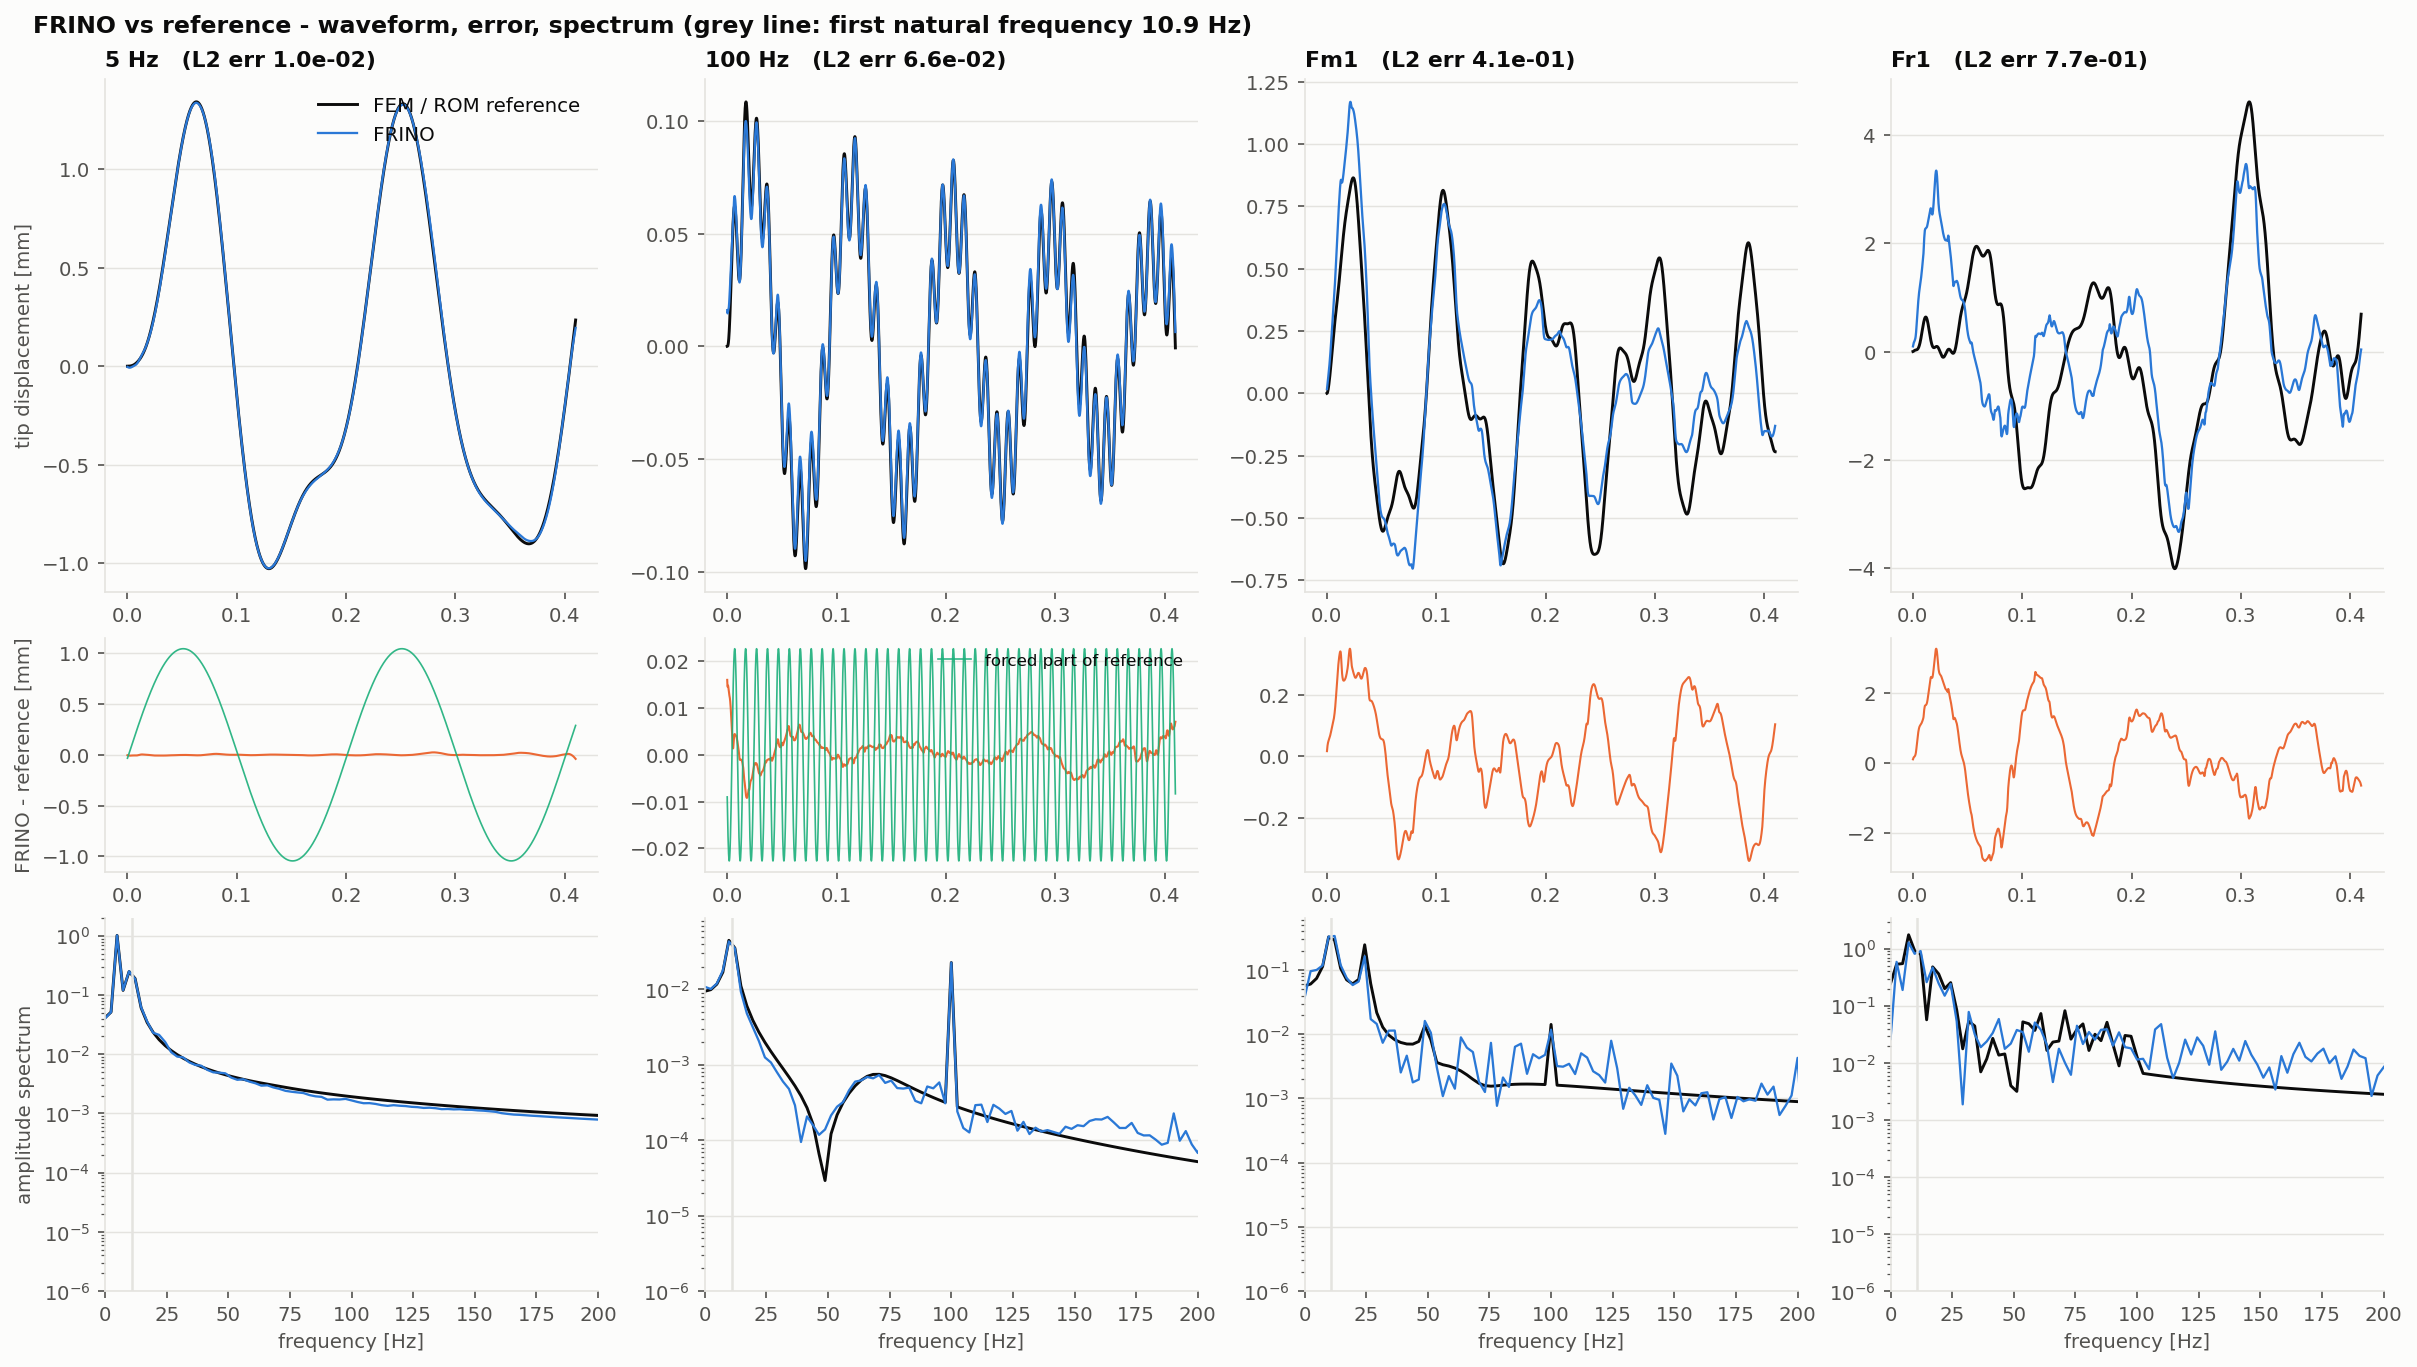
\includegraphics[width=0.98\linewidth]{figures/ch14r/fr_resp.png}
\caption{Tip displacement, operator-minus-reference error and amplitude spectrum for 5~Hz, 100~Hz, Fm1 and Fr1. At 5 and 100~Hz the waveforms are nearly indistinguishable and the 100~Hz forced peak is reproduced in the spectrum; on Fm1 and Fr1 the early-time peaks are missed.}\label{fig:vf-fr-resp}
\end{figure}

\emph{Why the high-frequency error looks large in the publication.} \Cref{tab:vf-fr-forced} splits the ROM response into forced and transient parts. Above about 90~Hz the forced response carries only $7$--$11\,\%$ of the energy, because the 10~Hz free-decay transient dominates the $L_2$ norm; a model that missed the forced part entirely would show $0.26$--$0.33$, exactly the publication's $0.29$--$0.31$. The network here reproduces the forced peak at the excitation frequency to $0.46\,\%$ at all eight tones. The publication's high-frequency errors are therefore consistent with a network that has not learned the forced response, and a whole-window $L_2$ norm hides this.

\begin{table}[tbp]
\centering\footnotesize
\setlength{\tabcolsep}{3pt}
\caption{Forced against transient split of the 3-mode ROM response.}\label{tab:vf-fr-forced}
\begin{tabular}{@{}lrrrrrr@{}}
\toprule
Tone & Forced energy fraction & Floor if forced part missed & Error & Error / forced norm & Spectral-peak error at $f_{\rm exc}$ & Error above 40 Hz\\
\midrule
5 Hz & 0.918 & 0.958 & $1.01\times10^{-2}$ & $1.06\times10^{-2}$ & $3.1\times10^{-4}$ & ---\\
10 Hz & 1.154 & 1.000 & $6.17\times10^{-3}$ & $5.74\times10^{-3}$ & $5.2\times10^{-4}$ & ---\\
15 Hz & 0.488 & 0.699 & $1.81\times10^{-2}$ & $2.60\times10^{-2}$ & $1.1\times10^{-3}$ & ---\\
20 Hz & 0.360 & 0.600 & $2.62\times10^{-2}$ & $4.36\times10^{-2}$ & $1.2\times10^{-3}$ & ---\\
95 Hz & 0.107 & 0.328 & $6.27\times10^{-2}$ & $1.91\times10^{-1}$ & $2.2\times10^{-3}$ & $6.01\times10^{-2}$\\
100 Hz & 0.089 & 0.299 & $6.56\times10^{-2}$ & $2.20\times10^{-1}$ & $1.7\times10^{-3}$ & $5.60\times10^{-2}$\\
105 Hz & 0.076 & 0.275 & $6.97\times10^{-2}$ & $2.53\times10^{-1}$ & $4.6\times10^{-3}$ & $5.90\times10^{-2}$\\
110 Hz & 0.065 & 0.256 & $1.43\times10^{-1}$ & $5.59\times10^{-1}$ & $1.7\times10^{-3}$ & $6.30\times10^{-2}$\\
\bottomrule
\end{tabular}
\end{table}

\subsection*{Results: training set, seeds and linearity}

\emph{Training set and seed noise.} \Cref{tab:vf-fr-train} and \Cref{fig:vf-fr-train} give the mean error by load class for three training sets. Broader training data improves the multi-frequency case (0.128 with 200 mixed waveforms against 0.443 with 40 tones) but costs in-range accuracy and training time; \Cref{tab:vf-fr-seed} and \Cref{fig:vf-fr-seed} show that in-range errors are stable across seeds ($1.5$--$2.0\times10^{-2}$ and $8$--$10\times10^{-2}$) while the multi-frequency error ranges from $0.215$ to $0.443$ for the same configuration, so differences below a factor of two in that column, here or in the publication's single runs, are not evidence of anything. The broad set's $0.128$ is a single run, about $1.7$ times below the best default seed.

\begin{table}[tbp]
\centering\footnotesize
\caption{Mean error by load class for three training sets.}\label{tab:vf-fr-train}
\begin{tabular}{@{}lrrrrr@{}}
\toprule
Training set & 5--20 Hz & 95--110 Hz & Multi-frequency & Random & Train time (s)\\
\midrule
8 paper tones & $3.1\times10^{-2}$ & $2.0\times10^{-1}$ & 0.619 & 0.928 & 46\\
40 single tones (default) & $1.5\times10^{-2}$ & $8.5\times10^{-2}$ & 0.443 & 0.691 & 202\\
200 mixed waveforms & $3.7\times10^{-2}$ & $2.8\times10^{-1}$ & 0.128 & 0.447 & 932\\
Publication (not stated) & $1.8\times10^{-2}$ & $3.0\times10^{-1}$ & 0.166 & 0.0976 & 1087\\
\bottomrule
\end{tabular}
\end{table}

\begin{figure}[tbp]
\centering
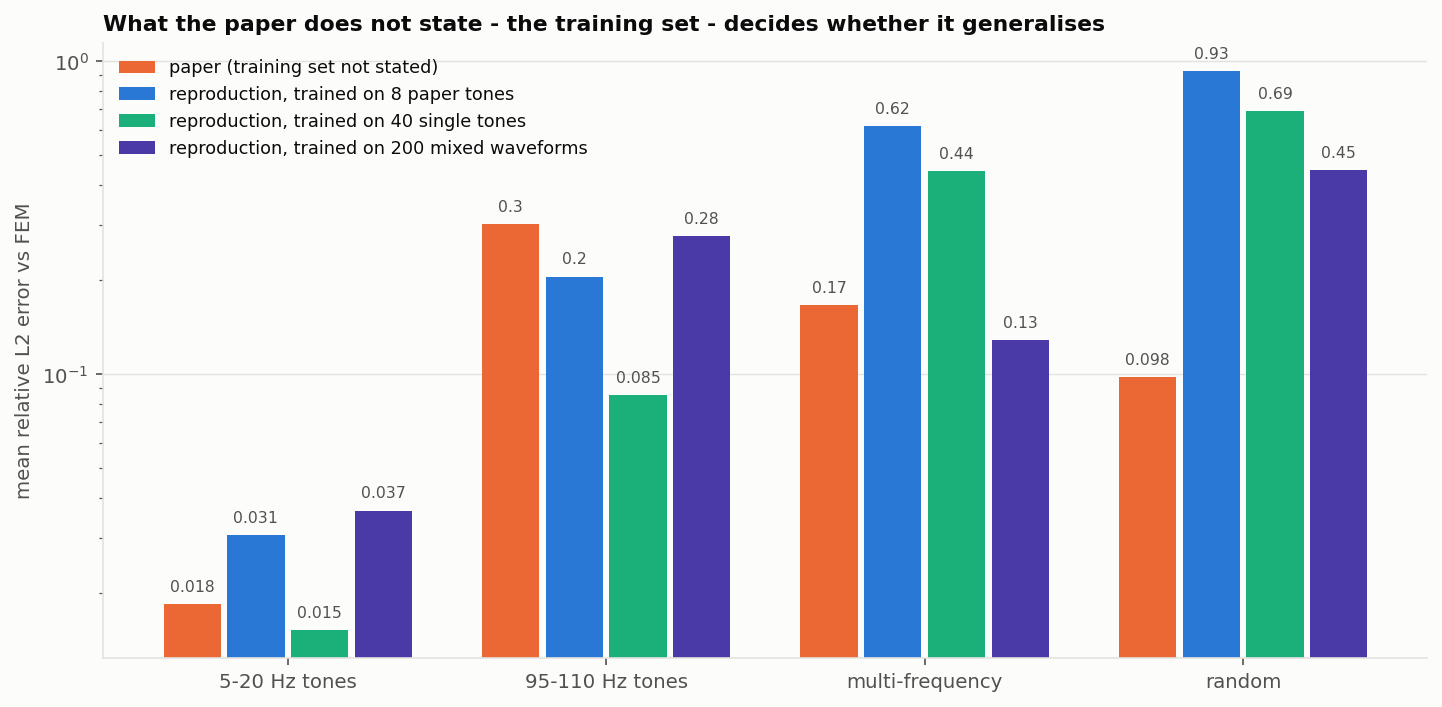
\includegraphics[width=0.7\linewidth]{figures/ch14r/fr_train.png}
\caption{Mean error by load class for three training sets and the publication's values.}\label{fig:vf-fr-train}
\end{figure}

\begin{table}[tbp]
\centering\footnotesize
\caption{Three seeds of the default configuration.}\label{tab:vf-fr-seed}
\begin{tabular}{@{}rrrrr@{}}
\toprule
Seed & 5--20 Hz & 95--110 Hz & Multi-frequency & Random\\
\midrule
0 & $1.51\times10^{-2}$ & $8.53\times10^{-2}$ & 0.443 & 0.691\\
1 & $1.56\times10^{-2}$ & $8.38\times10^{-2}$ & 0.215 & 0.699\\
2 & $1.98\times10^{-2}$ & $1.05\times10^{-1}$ & 0.297 & 0.640\\
\bottomrule
\end{tabular}
\end{table}

\begin{figure}[tbp]
\centering
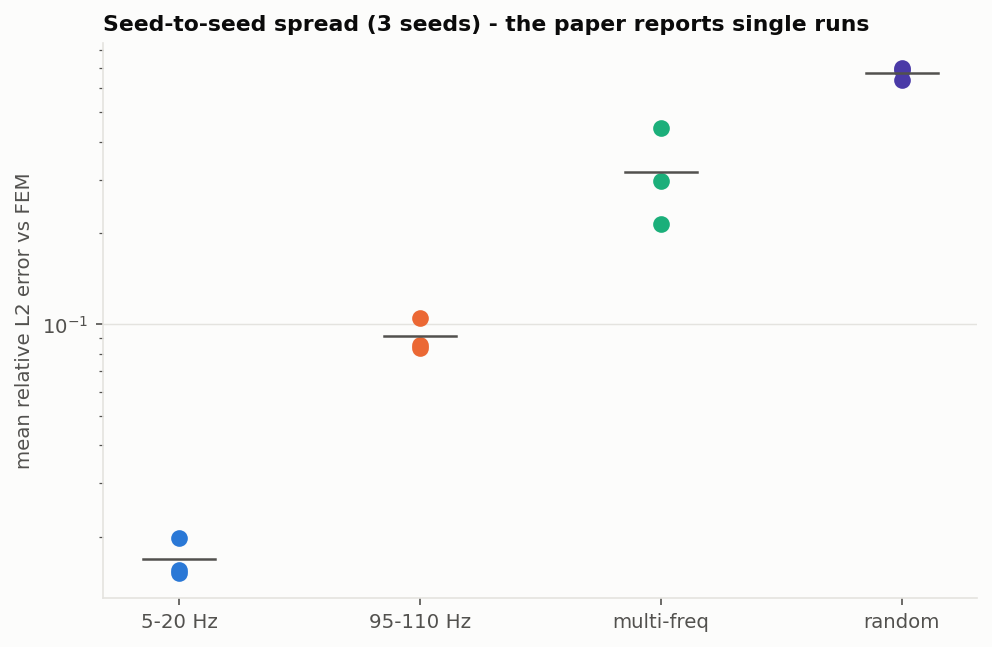
\includegraphics[width=0.7\linewidth]{figures/ch14r/fr_seed.png}
\caption{Three seeds of the default configuration.}\label{fig:vf-fr-seed}
\end{figure}

\emph{Is the learned operator linear?} The ROM operator is linear, so its superposition defect is zero; the trained network's mean superposition defect over 12 pairs of tones is $0.632$, and pairs with a tone at 95~Hz or above reach $1.0$--$1.2$. Scaling the 100~Hz waveform in amplitude shows the same (\Cref{tab:vf-fr-lin}, \Cref{fig:vf-fr-lin}): the relative error is $0.0695$ at the trained amplitude and $0.976$ at ten times that amplitude. The network interpolates between trained waveforms and amplitudes and has not learned the linearity of the structure, which is why waveform and amplitude generalisation depend on the training set.

\begin{table}[tbp]
\centering\footnotesize
\caption{Relative error of the 100~Hz tone for scaled amplitude (network trained at 10~N).}\label{tab:vf-fr-lin}
\begin{tabular}{@{}rrrrrr@{}}
\toprule
Amplitude factor & 0.01 & 0.1 & 1 & 10 & 100\\
\midrule
Relative error & 53.1 & 4.84 & 0.0695 & 0.976 & 1.06\\
\bottomrule
\end{tabular}
\end{table}

\begin{figure}[tbp]
\centering
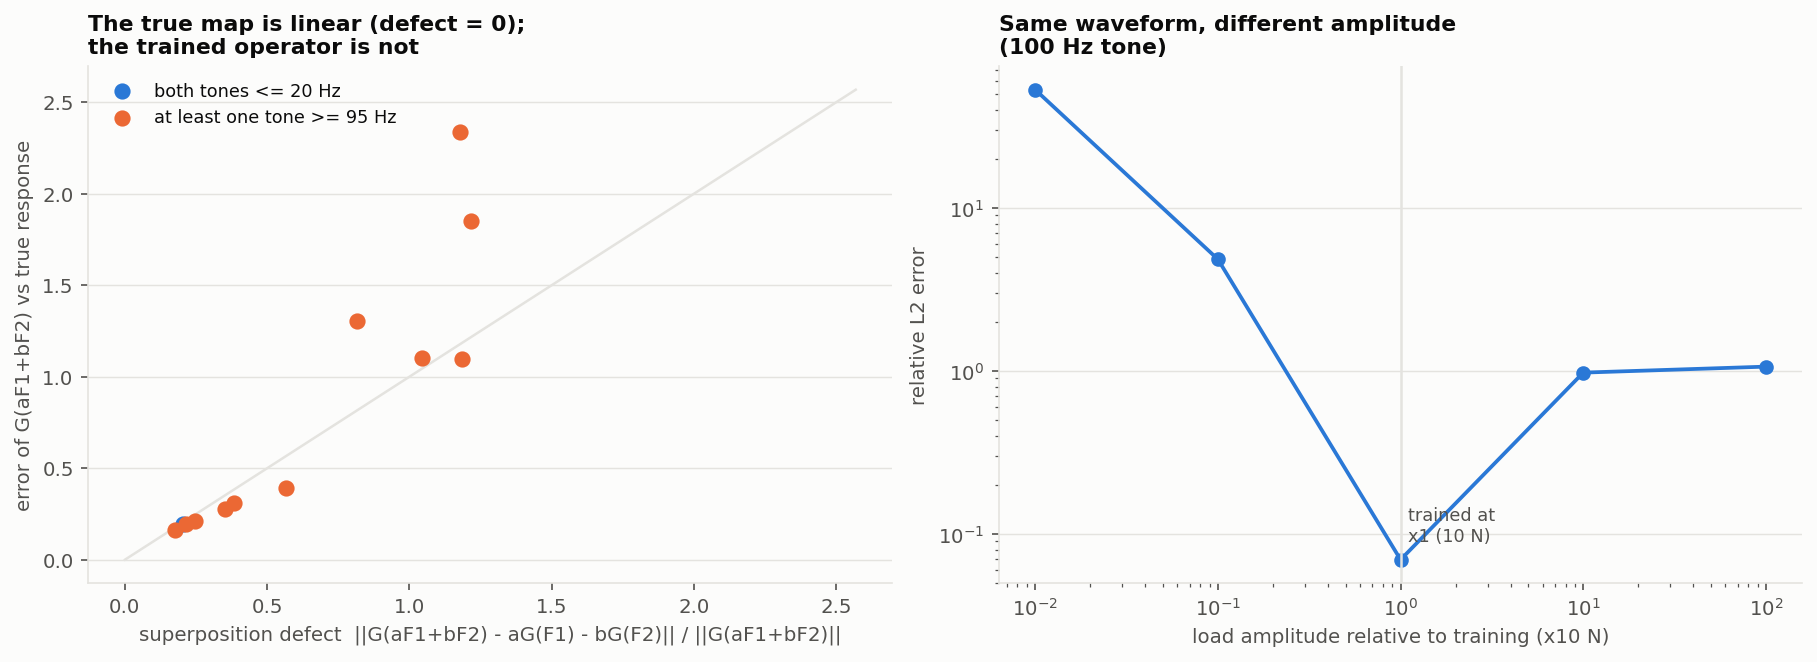
\includegraphics[width=0.9\linewidth]{figures/ch14r/fr_lin.png}
\caption{Left: superposition defect of the trained operator for random pairs of tones. Right: error for the same 100~Hz waveform scaled in amplitude.}\label{fig:vf-fr-lin}
\end{figure}

\subsection*{Results: parameter studies}

Every row trains a fresh network (500 epochs) and reports the mean error over load classes on the finer grid; differences below about $30\,\%$ on the in-range columns and a factor of two on the generalisation columns are within seed noise.

\emph{Physics weight.} \Cref{tab:vf-fr-lambda} and \Cref{fig:vf-fr-lambda}: the best in-range errors occur at small $\lambda$ ($10^{-6}$ to $10^{-3}$) and from $10^{-2}$ upward the 5--20~Hz error rises from $1.5\times10^{-2}$ to $2.6\times10^{-2}$. A data-only network ($\lambda=0$) is $3\,\%$ worse at 5--20~Hz and $21\,\%$ worse at 95--110~Hz than the default, both inside seed noise. With labels from the exact ROM the ROM residual is the same error re-weighted by the dynamic-stiffness operator and so carries no new information.

\begin{table}[tbp]
\centering\footnotesize
\caption{Effect of the physics weight $\lambda$.}\label{tab:vf-fr-lambda}
\begin{tabular}{@{}lrrrrrr@{}}
\toprule
$\lambda$ & 5--20 Hz & 95--110 Hz & Multi-frequency & Random & Final data loss & Final ROM loss\\
\midrule
0 (data only) & $1.56\times10^{-2}$ & $1.03\times10^{-1}$ & 0.37 & 0.66 & $4.3\times10^{-4}$ & ---\\
$10^{-6}$ & $1.53\times10^{-2}$ & $9.97\times10^{-2}$ & 0.369 & 0.66 & $4.2\times10^{-4}$ & $1.2$\\
$10^{-4}$ & $1.46\times10^{-2}$ & $8.62\times10^{-2}$ & 0.384 & 0.651 & $3.2\times10^{-4}$ & $1.3\times10^{-1}$\\
$10^{-3}$ (default) & $1.52\times10^{-2}$ & $8.53\times10^{-2}$ & 0.443 & 0.691 & $2.8\times10^{-4}$ & $3.7\times10^{-2}$\\
$10^{-2}$ & $2.22\times10^{-2}$ & $9.60\times10^{-2}$ & 0.368 & 0.781 & $4.2\times10^{-4}$ & $1.9\times10^{-2}$\\
$10^{-1}$ & $2.47\times10^{-2}$ & $8.54\times10^{-2}$ & 0.509 & 0.82 & $5.2\times10^{-4}$ & $7.8\times10^{-3}$\\
1 & $2.62\times10^{-2}$ & $1.44\times10^{-1}$ & 0.34 & 0.746 & $2.0\times10^{-3}$ & $2.5\times10^{-3}$\\
\bottomrule
\end{tabular}
\end{table}

\begin{figure}[tbp]
\centering
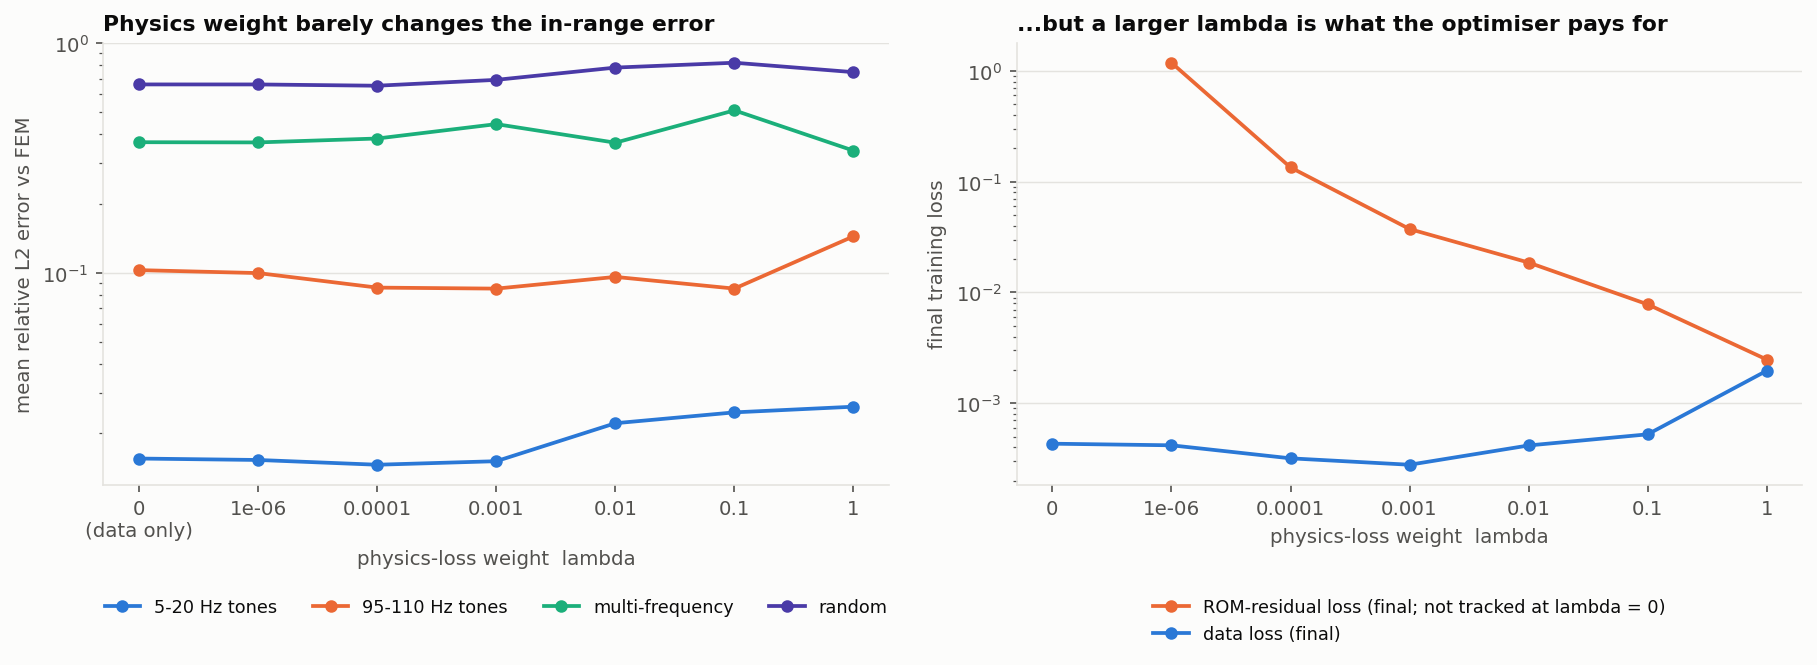
\includegraphics[width=0.9\linewidth]{figures/ch14r/fr_lambda.png}
\caption{Error against the physics weight $\lambda$.}\label{fig:vf-fr-lambda}
\end{figure}

\emph{Resolution, width and ROM order.} \Cref{tab:vf-fr-hyper} and \Cref{fig:vf-fr-hyper}: error falls up to 256--512 points per excitation and then stops improving while training time keeps rising (the publication's 6.25\,\% is on the knee); width 128 matches width 256 at $38\,\%$ of the training time; and the ROM order does not change accuracy, as the publication finds, but unlike its $1.1\times10^{3}$, $5.8\times10^{3}$, $1.6\times10^{4}$~s the training time is flat here because the cost is dominated by the width-256 Fourier layers and not by the number of reduced channels. The first-order forward difference that an analysis predicted to carry a 0.25~rad phase error at 100~Hz does not change the result at $\lambda=10^{-3}$, where the data loss dominates, and row scaling of the residual by $\operatorname{diag}(\mathbf K)$ makes the in-range error about $45\,\%$ worse by raising the effective weight of the physics term.

\begin{table}[tbp]
\centering\footnotesize
\caption{Resolution, width and ROM order (mean errors on the finer grid).}\label{tab:vf-fr-hyper}
\begin{tabular}{@{}llrrrr@{}}
\toprule
Parameter & Value & 5--20 Hz & 95--110 Hz & Multi-frequency & Train time (s)\\
\midrule
Points per excitation & 64 & $8.03\times10^{-2}$ & 1.24 & 0.469 & 68\\
 & 128 & $2.80\times10^{-2}$ & $2.15\times10^{-1}$ & 0.347 & 84\\
 & 256 & $1.72\times10^{-2}$ & $9.31\times10^{-2}$ & 0.367 & 102\\
 & 512 & $1.52\times10^{-2}$ & $8.53\times10^{-2}$ & 0.443 & 132\\
 & 1024 & $1.86\times10^{-2}$ & $9.94\times10^{-2}$ & 0.492 & 198\\
 & 2048 & $2.08\times10^{-2}$ & $1.07\times10^{-1}$ & 0.49 & 326\\
\addlinespace
Network width & 16 & $6.24\times10^{-2}$ & $2.38\times10^{-1}$ & 0.892 & 24\\
 & 32 & $3.68\times10^{-2}$ & $1.78\times10^{-1}$ & 0.859 & 22\\
 & 64 & $2.06\times10^{-2}$ & $1.32\times10^{-1}$ & 0.664 & 32\\
 & 128 & $1.34\times10^{-2}$ & $8.99\times10^{-2}$ & 0.477 & 51\\
 & 256 & $1.52\times10^{-2}$ & $8.53\times10^{-2}$ & 0.443 & 133\\
\addlinespace
ROM order & 3 & $1.52\times10^{-2}$ & $8.53\times10^{-2}$ & 0.443 & 133\\
 & 10 & $1.45\times10^{-2}$ & $1.22\times10^{-1}$ & 0.448 & 136\\
 & 20 & $2.39\times10^{-2}$ & $1.41\times10^{-1}$ & 0.438 & 139\\
\bottomrule
\end{tabular}
\end{table}

\begin{figure}[tbp]
\centering
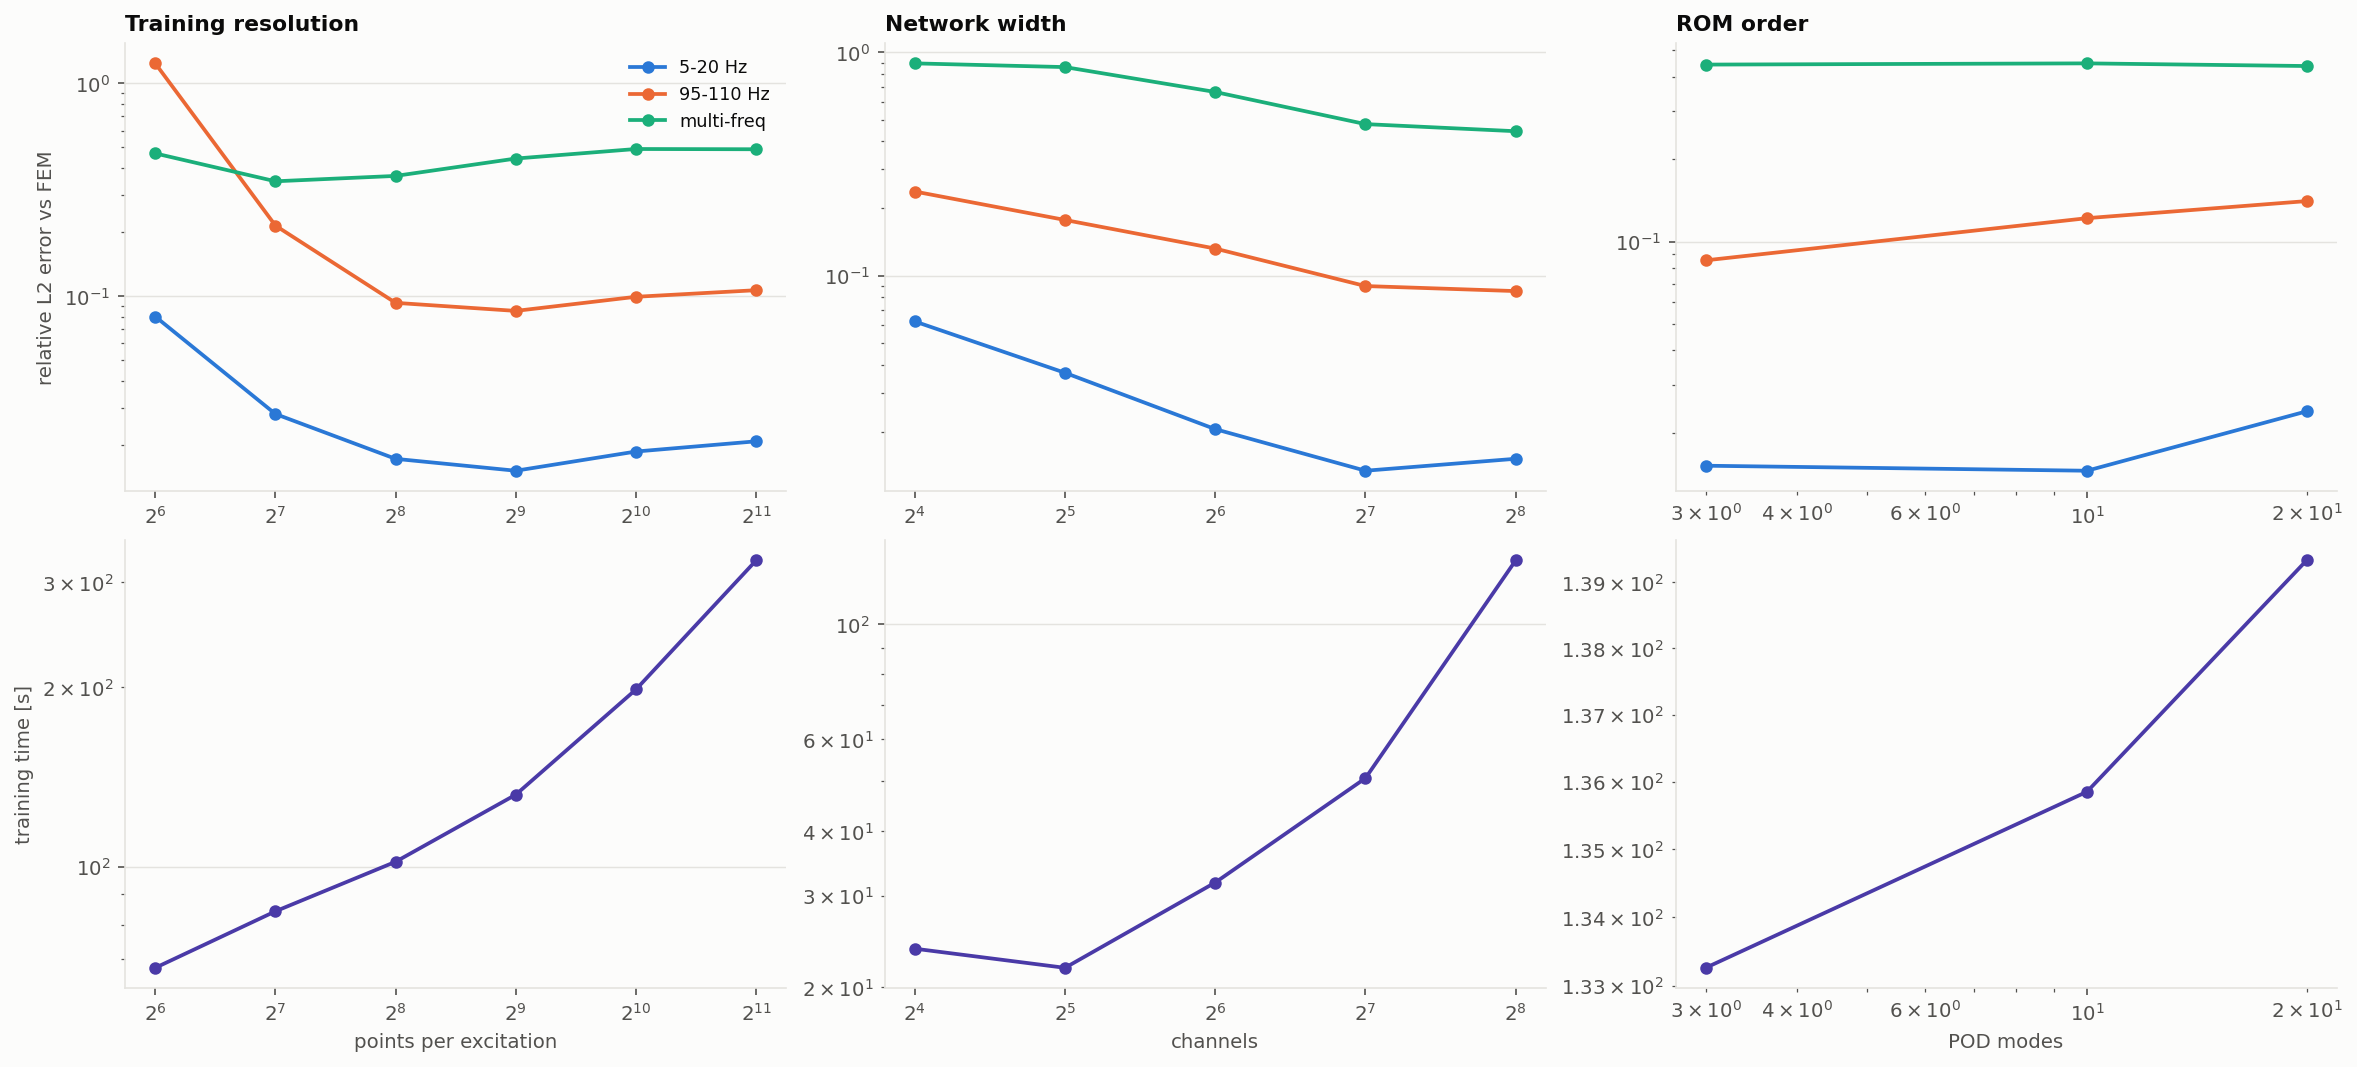
\includegraphics[width=0.98\linewidth]{figures/ch14r/fr_hyper.png}
\caption{Error and training time against the training resolution, the network width and the ROM order.}\label{fig:vf-fr-hyper}
\end{figure}

\subsection*{Results: PINN baselines and cost}

The publication gives no architecture, collocation set or budget for its PINN, so the baselines are the author's designs. The first attempt (1500 iterations) uses soft initial conditions, equal fixed loss weights, 500 fixed collocation points, random Fourier features with $\sigma=40$ and an output scale of 5 times the static deflection. The tuned version (3000 iterations) uses hard initial conditions $q=q_st^2N(t)$, 2048 resampled collocation points, gradient-norm loss balancing, a Fourier-feature scale $\sigma=f_{\rm exc}T/2$, an output scale from linear vibration theory, forward-mode differentiation and an L-BFGS polish; variants with labels use the ROM solution at the 6.25\,\% training points. \Cref{tab:vf-fr-pinn} and \Cref{fig:vf-fr-pinn} give the errors. First-attempt baselines are at about 1.0 (no learning) from 20~Hz upward, with or without labels; tuning gives 3 to 30 times lower error at 5~Hz and makes Fourier features and labels help, but not above 20~Hz without labels; with tuning and labels the best baseline reaches $0.30$--$0.38$ at 20--110~Hz and the operator is $2.7$ to $11$ times more accurate there. The publication's two orders of magnitude over a PINN is reached only against first-attempt PINNs ($38$--$44$ times at 5--20~Hz, 15 times at 100~Hz here); a stronger PINN setup might narrow the gap, and each configuration is one run.

\begin{table}[tbp]
\centering\footnotesize
\caption{Relative $L_2$ error of per-tone PINN baselines against the FEM.}\label{tab:vf-fr-pinn}
\begin{tabular}{@{}llrrrrr@{}}
\toprule
Tone & Setup & PINN & FF-PINN & PINN + data & FF-PINN + data & Operator\\
\midrule
5 Hz & first attempt & 0.446 & 0.999 & 0.433 & 0.999 & ---\\
5 Hz & tuned & 0.136 & 0.0457 & 0.0604 & 0.0298 & 0.0101\\
20 Hz & first attempt & 0.991 & 0.997 & 0.991 & 0.997 & ---\\
20 Hz & tuned & 1.17 & 0.793 & 0.923 & 0.297 & 0.0262\\
100 Hz & first attempt & 1.01 & 1.01 & 1.01 & 1.01 & ---\\
100 Hz & tuned & 1.01 & 0.897 & 0.575 & 0.38 & 0.0657\\
110 Hz & first attempt & 0.996 & 0.983 & 0.995 & 0.982 & ---\\
110 Hz & tuned & 0.985 & 0.92 & 0.567 & 0.38 & 0.143\\
\bottomrule
\end{tabular}
\end{table}

\begin{figure}[tbp]
\centering
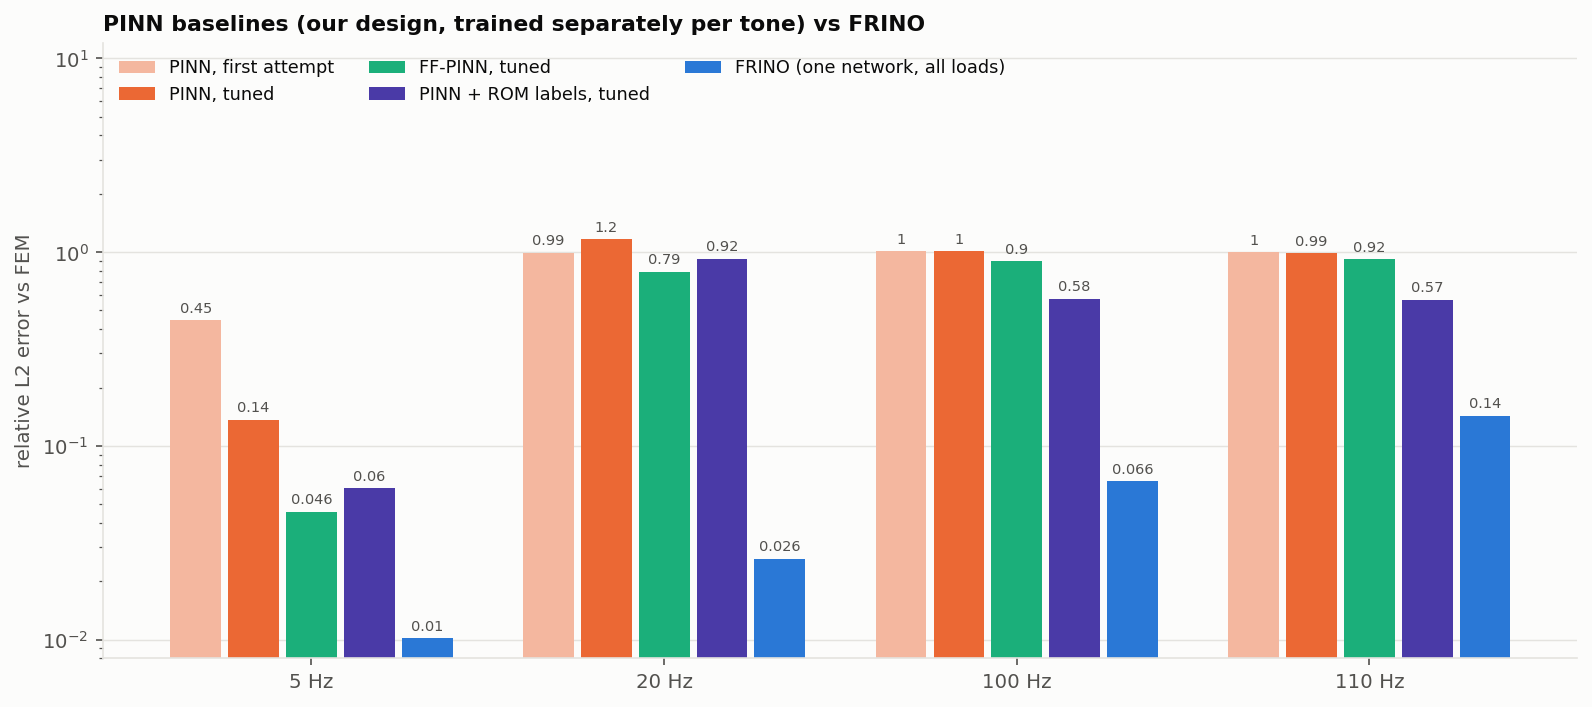
\includegraphics[width=0.9\linewidth]{figures/ch14r/fr_pinn.png}
\caption{Per-tone PINN baselines against the operator.}\label{fig:vf-fr-pinn}
\end{figure}

\emph{Cost.} \Cref{tab:vf-fr-cost} and \Cref{fig:vf-fr-cost}: for this linear benchmark the exact frequency-domain solution of the publication's Eq.~(20) costs $18.1$~ms, the same order as the operator's inference ($11$~ms), so its $139$~s of training is never repaid against it (break-even about $2\times10^{4}$ loads); against the CPU full-order solve the break-even is about 3 loads, and against ROM time stepping about 16 (overstated, since that GPU time stepping is launch-bound and a CPU loop is faster). A fair speed claim for this linear problem must compare with the frequency-domain solve; the 4580~s of finite element time in the publication's Table~2 is about 100 times slower than the solve here, which inflates its ratio.

\begin{table}[tbp]
\centering\footnotesize
\caption{Seconds per excitation on the study machine.}\label{tab:vf-fr-cost}
\begin{tabular}{@{}lr@{}}
\toprule
Method & Time per excitation\\
\midrule
FOM Newmark, CPU SuperLU (4032 free dofs, 8192 steps; extrapolated from 300 steps) & 47.0 s\\
FOM Newmark, GPU, batch of 12 (per load) & 17.2 s\\
ROM Newmark (3 modes, GPU; kernel-launch bound) & 8.45 s\\
ROM exact frequency-domain solve, Eq.~(20) (GPU) & 18.1 ms\\
Operator inference (512 points, GPU) & 11.0 ms\\
Operator training (once) & 139 s\\
\bottomrule
\end{tabular}
\end{table}

\begin{figure}[tbp]
\centering
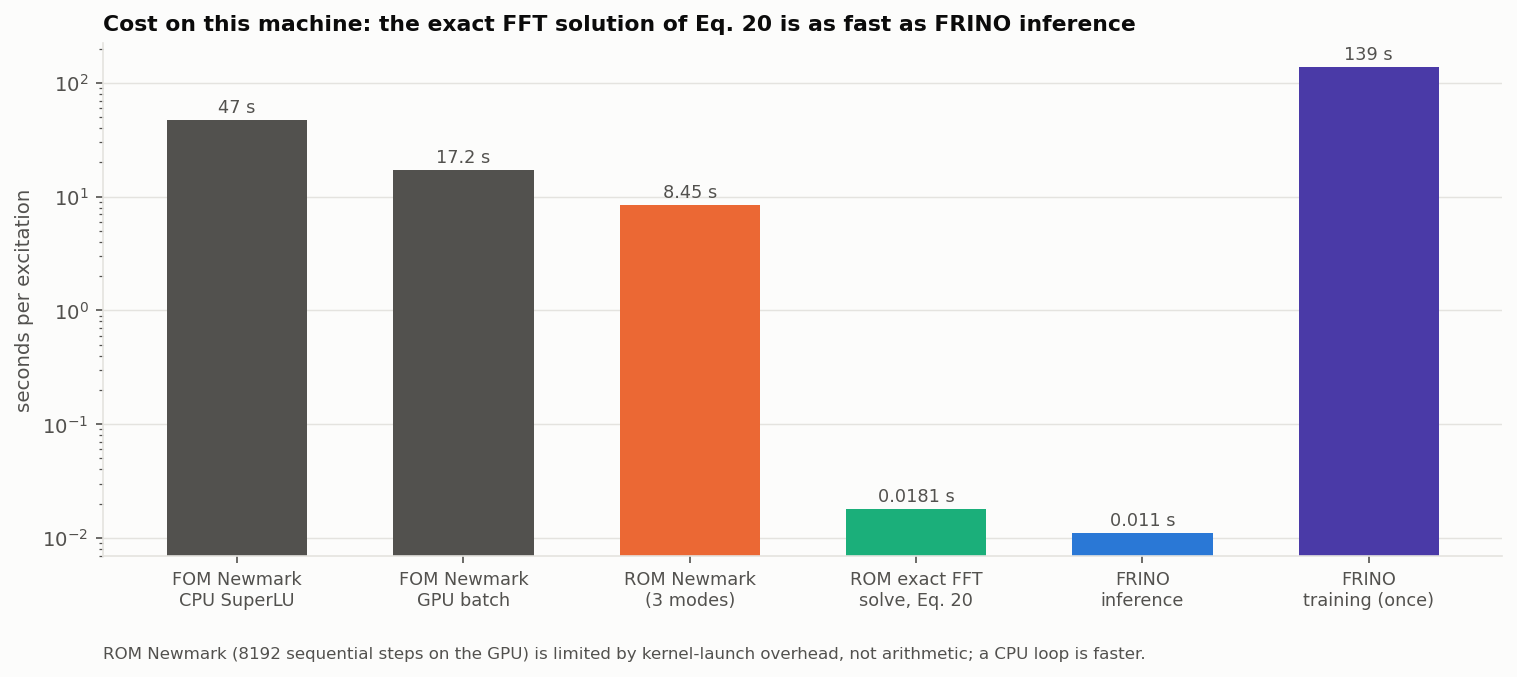
\includegraphics[width=0.7\linewidth]{figures/ch14r/fr_cost.png}
\caption{Seconds per excitation on the study machine.}\label{fig:vf-fr-cost}
\end{figure}

\begin{figure}[tbp]
\centering
\includegraphics[width=0.7\linewidth]{figures/ch14_frino.pdf}
\caption{Neural operator of \citet{yang2025frino}: mean relative error for single tones at low and high frequency, multi-frequency loads and random loads, for three training sets. Dashed lines are the publication's values. With 40 tones the multi-frequency and random errors are \cvfFrinoMulti{} and \cvfFrinoRandom.}\label{fig:vf-frino}
\end{figure}

\subsection*{Comparison with the publication}

\begin{table}[tbp]
\centering\footnotesize
\caption{Claims of \citet{yang2025frino} and the outcome of the reproduction.}\label{tab:vf-fr-cmp}
\begin{tabularx}{\linewidth}{@{}>{\raggedright\arraybackslash}p{4.2cm} >{\raggedright\arraybackslash}X >{\raggedright\arraybackslash}p{2.5cm}@{}}
\toprule
Claim & This work & Outcome\\
\midrule
Accurate low-frequency single tones ($\sim10^{-2}$) & $1.5\times10^{-2}$ mean over 5--20 Hz & reproduced\\
High-frequency errors $\sim0.3$ & $8.5\times10^{-2}$ over 95--110 Hz; the 0.3 equals the error of not learning the forced response & not matched (lower)\\
Multi-frequency and random loads without retraining (0.10--0.20) & 0.443 and 0.691 with 40 tones; best 0.128 and 0.447 with 200 waveforms & not reproduced\\
Learns the natural-frequency content & spectral-peak error at $f_1\le0.115$ & reproduced (in-range tones)\\
Up to 100$\times$ more accurate than a PINN & $37.9\times$ against a first-attempt PINN at 20 Hz; $2.66$--$11.4\times$ against tuned & only against a weak PINN\\
Up to 1000$\times$ faster than a PINN & both milliseconds at inference; a PINN is retrained per load & not meaningful as stated\\
$10^6\times$ faster than FEM & $4265\times$ against the CPU full-order solve (47 s; publication's 4580 s) & partly\\
Zero-shot super-resolution; 6.25\,\% data enough & 16$\times$ finer grid changes tone errors by $<2\times$; plateau from 256--512 points & reproduced\\
$\lambda\le10^{-2}$ appropriate & consistent, but the term has little effect & consistent\\
Width 128--256 optimal; wider overfits & plateau reproduced; no width $>256$ run & overfitting untested\\
Higher ROM order costs more training time & accuracy claim reproduced; training time flat & time claim not\\
\bottomrule
\end{tabularx}
\end{table}

\subsection*{What the missing data prevent}

The ANSYS model, the publication's training set and its code are unavailable, so exact numbers cannot be matched; every unstated choice is in \Cref{tab:vf-fr-setup}. Each configuration was trained once except for the three seeds, and differences below the seed spread are not significant. The operator was trained in single precision on a 3~GB GPU; a double-precision run with the package's own FNO blocks is supported but was not run. The PINN baselines are the author's designs, and no width above 256 was run, so the publication's overfitting-with-width claim is untested. An analysis written before the runs made predictions that the outcomes confirmed (consistent units give 345~Hz against $10.9$~Hz as printed; $\zeta_1=2.8\,\%$ against the estimated $2.6\,\%$; the exact frequency-domain solve costs $18$~ms against $11$~ms; the publication's $30\,\%$ high-frequency error equals the forced-part floor; the superposition defect is $0.63$) or contradicted (scale-free residual rows did not help; the estimated third-mode frequency of 175~Hz is 227.8~Hz in the three-dimensional ROM; the forward-difference effect is not visible in the final accuracy).


\section{Hybrid hyper-reduction for contact}\label{sec:vf-hyb}

\subsection*{Concept and purpose}

\citet{fauque2018hybrid} reduce a frictionless contact problem by keeping the \emph{displacements} in a reduced basis while the contact forces (the Lagrange multipliers) on a reduced integration domain (RID) stay finite element unknowns, which is why the model is called hybrid. Signorini conditions then hold exactly at the contact points of the RID, and no compressed basis of non-negative multipliers is needed. The RID is built from discrete empirical interpolation points of the displacement basis, and a greedy loop driven by a solve-free error indicator chooses the training parameters. The paper tests the method on a one-dimensional rope against an obstacle and on a three-dimensional pellet--cladding problem. The study rebuilds both and compares with the projection-based method of \Cref{sec:vf-bal} (the ``PB'' method) at equal accuracy.

The study uses the contact solvers of \fea{} (\anchor{fea_engine.contact_solvers}) for the full-order problem and the existing \rom{} building blocks (POD, \anchor{rom_engine.deim_indices}, inf-sup enrichment, \anchor{rom_engine.reconstruct_contact_forces}, the PB method with a non-negative dual basis). The hybrid solve itself, with the RID construction, the restricted full-order problem on the RID and the indicator $\eta$, is new code written for this study and now in \rom{} as \anchor{rom_engine.contact_rid} (with eight unit tests).

\subsection*{Mathematics as implemented}

\emph{Full-order problem.} A discretised frictionless contact problem is the saddle-point system
\begin{equation}\label{eq:hb-fom}
\mathbf K\mathbf U+\mathbf B^{T}\boldsymbol\Lambda=\mathbf F,\qquad\mathbf B\mathbf U\le\mathbf D,\qquad\boldsymbol\Lambda\ge\mathbf 0,\qquad\boldsymbol\Lambda\odot(\mathbf B\mathbf U-\mathbf D)=\mathbf 0,
\end{equation}
with $\mathbf K\in\mathbb R^{N\times N}$ the stiffness, $\mathbf B$ the gap matrix, $\mathbf D$ the initial gap and $\odot$ the element-wise product. \fea{} uses the opposite sign convention ($\mathbf K\mathbf u=\mathbf f+\mathbf B^{T}\boldsymbol\lambda$, $\mathbf B\mathbf u\ge\mathbf c$), so the scripts call it with $\mathbf B\to-\mathbf I$, $\mathbf c\to-\mathbf D$.

\emph{Basis and RID.} The primal basis $\mathbf V\in\mathbb R^{N\times l_u}$ is a POD of the snapshots, keeping the smallest $l_u$ whose information rate reaches $1-\epsilon_{\rm tol}$,
\begin{equation}\label{eq:hb-rate}
\tau(l_u)=\frac{\sum_{j\le l_u}\sigma_j^2}{\sum_j\sigma_j^2}\ge1-\epsilon_{\rm tol}.
\end{equation}
Discrete empirical interpolation selects $l_u$ indices from $\mathbf V$ (and from a coarse POD of the multiplier snapshots, so that the contact zone is represented); the RID is the union of the element supports of these degrees of freedom, optionally enlarged by rings of neighbouring elements. Let $\mathcal P$ be the degrees of freedom all of whose incident elements lie in the RID (their balance equations can be written exactly there), $\mathcal E$ all degrees of freedom of RID elements, $\Gamma_I=\mathcal E\setminus\mathcal P$ the interface, and $\mathcal C_\lambda$ the contacts whose gap is computable from $\mathcal P$.

\emph{Hybrid reduced problem.} With the enriched basis $\bar{\mathbf V}$ below, the reduced problem is a Petrov--Galerkin system
\begin{equation}\label{eq:hb-red}
\begin{cases}
\bar{\mathbf V}[\mathcal P,:]^{T}\mathbf K[\mathcal P,\mathcal E]\,\bar{\mathbf V}[\mathcal E,:]\,\boldsymbol\gamma+(\mathbf B[\mathcal C_\lambda,:]\bar{\mathbf V})^{T}\boldsymbol\Lambda[\mathcal C_\lambda]=\bar{\mathbf V}[\mathcal P,:]^{T}\mathbf F[\mathcal P],\\[2pt]
\boldsymbol\Lambda[\mathcal C_\lambda]\odot(\mathbf B[\mathcal C_\lambda,:]\bar{\mathbf V}\boldsymbol\gamma-\mathbf D[\mathcal C_\lambda])=\mathbf 0,\quad
\mathbf B[\mathcal C_\lambda,:]\bar{\mathbf V}\boldsymbol\gamma\le\mathbf D[\mathcal C_\lambda],\quad\boldsymbol\Lambda[\mathcal C_\lambda]\ge\mathbf 0 ,
\end{cases}
\end{equation}
with the displacement $\mathbf U=\bar{\mathbf V}\boldsymbol\gamma$ on the whole domain. The reduced matrix $\mathbf A=\bar{\mathbf V}[\mathcal P,:]^{T}\mathbf K[\mathcal P,\mathcal E]\bar{\mathbf V}[\mathcal E,:]$ is not symmetric. Eliminating $\boldsymbol\gamma$ gives the condensed complementarity problem solved online with Lemke's algorithm,
\begin{equation}\label{eq:hb-lcp}
\boldsymbol\gamma=\mathbf A^{-1}(\mathbf b-\mathbf B_r^{T}\boldsymbol\Lambda),\qquad
\mathbf w=(\mathbf D-\mathbf B_r\mathbf A^{-1}\mathbf b)+(\mathbf B_r\mathbf A^{-1}\mathbf B_r^{T})\boldsymbol\Lambda\ge\mathbf 0,\quad\boldsymbol\Lambda\ge\mathbf 0,\quad\boldsymbol\Lambda^{T}\mathbf w=0,
\end{equation}
with $\mathbf b=\bar{\mathbf V}[\mathcal P,:]^{T}\mathbf F[\mathcal P]$ and $\mathbf B_r=\mathbf B[\mathcal C_\lambda,:]\bar{\mathbf V}$; a plain active-set loop on the saddle system \cref{eq:hb-red} picks wrong contact sets ($\operatorname{cond}(\mathbf A)\approx10^{14}$).

\emph{Inf-sup condition.} Well-posedness needs $\mathbf B_r$ to have full row rank (a necessary condition is $\bar l_u\ge N^C_\lambda$). If it fails, unit vectors at contact degrees of freedom are appended,
\begin{equation}\label{eq:hb-enrich}
\bar{\mathbf V}=\big[\mathbf V\ \big|\ \mathbf I_N[:,i^c_1],\dots,\mathbf I_N[:,i^c_{\bar l_u-l_u}]\big],
\end{equation}
so part of the primal field is treated with full-order functions at the contact degrees of freedom.

\emph{Reconstruction outside the RID.} The reduced model returns $\boldsymbol\Lambda$ only on $\mathcal C_\lambda$; outside it a non-negative least-squares fit over multiplier snapshots $\mathbf S_\lambda$ is used,
\begin{equation}\label{eq:hb-nnls}
\min_{\boldsymbol\gamma_\lambda\ge0}\Big\lVert\begin{pmatrix}\mathbf S_\lambda[\mathcal C_\lambda,:]\\ [\mathbf B\mathbf U-\mathbf D]_{-}\odot\mathbf S_\lambda\end{pmatrix}\boldsymbol\gamma_\lambda-\begin{pmatrix}\boldsymbol\Lambda[\mathcal C_\lambda]\\\mathbf 0\end{pmatrix}\Big\rVert_2^2,\qquad\boldsymbol\Lambda=\mathbf S_\lambda\boldsymbol\gamma_\lambda,
\end{equation}
the first block matching the RID multipliers and the second penalising force where the gap is open.

\emph{Indicator and greedy sampling.} For a new parameter $\mu$ the snapshot displacements on $\Gamma_I$ are interpolated in parameter space, $\tilde{\mathbf U}(\mu)[\Gamma_I]=\sum_\rho\alpha_\rho(\mu)\mathbf U(\rho)[\Gamma_I]$, and the full-order problem written only on the RID is solved with this Dirichlet data,
\begin{equation}\label{eq:hb-restr}
\mathbf K[\mathcal P,\mathcal P]\tilde{\mathbf U}_{\mathcal P}+\mathbf B_{\mathcal P}^{T}\tilde{\boldsymbol\Lambda}=\mathbf F[\mathcal P]-\mathbf K[\mathcal P,\Gamma_I]\tilde{\mathbf U}_{\Gamma_I},\qquad\mathbf B_{\mathcal P}\tilde{\mathbf U}_{\mathcal P}\le\mathbf D-\mathbf B_I\tilde{\mathbf U}_{\Gamma_I}.
\end{equation}
The indicator is the relative discrepancy of the hyper-reduced and the restricted solutions,
\begin{equation}\label{eq:hb-eta}
\eta(\mu)=\frac{\lVert(\mathbf U^{hr}-\tilde{\mathbf U})[\mathcal P]\rVert_{H^1}}{\lVert\tilde{\mathbf U}[\mathcal P]\rVert_{H^1}}+\frac{\lVert\boldsymbol\Lambda^{hr}-\tilde{\boldsymbol\Lambda}\rVert_{(H^1)'}}{\lVert\tilde{\boldsymbol\Lambda}\rVert_{(H^1)'}},\qquad\lVert x\rVert_{(H^1)'}=\sqrt{x^{T}\mathbf M_{H^1}^{-1}x},
\end{equation}
which needs no full-order solve at the candidate. The greedy loop takes $\mu^\star=\arg\max\eta$, computes the full-order solution there, rebuilds POD, RID and basis (the RID may only grow) and repeats. The comparison method (PB) is a Galerkin projection on a POD primal basis $\mathbf V_u$ and a non-negative matrix factorisation dual basis $\mathbf V_\lambda\ge0$ of the same size, with the non-penetration violation $I(\mu)=\lVert[\mathbf B\mathbf V\boldsymbol\gamma-\mathbf D]_+\rVert_2$ as greedy indicator.

\subsection*{Geometry and mesh: the one-dimensional rope}

The rope is an elastic string on $[0,1]$ with 100 linear nodes (98 free), $u(0)=u(1)=0$ and the obstacle constraint $u\le d$ (\Cref{fig:vf-hb-geom}):
\begin{equation}\label{eq:hb-rope}
-(\nu u')'=f,\quad\nu(x,\mu_1)=\mu_1\mathbf 1_{[0,0.5]}+0.15\,\mathbf 1_{]0.5,1]},\quad d(x,\mu_2)=0.2(\sin\pi x-\sin3\pi x)+0.5-\mu_2(x-0.5),
\end{equation}
with parameters $\mu=(\mu_1,\mu_2)\in[0.05,0.25]\times[-0.05,0.5]$. The stiffness is affine in $\mu_1$, $\mathbf K(\mu)=\mu_1\mathbf K_a+0.15\mathbf K_b$, so $\mathbf K[\mathcal P,\mathcal E]$ is formed online from two precomputed slices. The publication states $f=-1$; with $u\le d$ and $d>0$ everywhere that load pushes the rope away from the obstacle and no contact occurs, so $f=+1$ is used (the mirror image $u\to-u$ of the publication's problem), the only way the contact patterns of its figures can appear.

\begin{figure}[tbp]
\centering
\includegraphics[width=0.98\linewidth]{figures/ch14_geom_rope.pdf}
\caption{Rope obstacle problem of the study, drawn from \cref{eq:hb-rope}. (a) The rope, the load and the obstacle for three values of $\mu_2$. (b) The stiffness coefficient for three values of $\mu_1$.}\label{fig:vf-hb-geom}
\end{figure}

\begin{table}[tbp]
\centering\footnotesize
\caption{Model size of the regular-grid study (10$\times$12 snapshots), against the publication.}\label{tab:vf-hb-size}
\begin{tabular}{@{}lrr@{}}
\toprule
 & This work & Publication\\
\midrule
Primal POD modes $l_u$ & 10 & 9\\
Dual POD modes used for the RID & 4 & 1\\
RID elements & 42 & ---\\
Balance / contact nodes in the RID & 36 & 14 contact nodes (28 RID nodes)\\
Finite element dofs added for inf-sup & 26 & 5\\
Unknowns (primal + multipliers) & 72 & 28\\
Inf-sup deficiency after enrichment & 0 & ---\\
\bottomrule
\end{tabular}
\end{table}

The dual mode count differs because the first multiplier mode holds only $67\,\%$ of the multiplier energy in this implementation (energy rates $0.67$, $0.84$, $0.89$, $0.92$), so no information-rate variant yields one mode at $\epsilon=0.1$; the publication's multiplier snapshots must be closer to rank one. A variant imposing one dual mode is reported alongside.

\subsection*{Results: the rope on a regular snapshot grid}

\emph{Basis decay.} \Cref{fig:vf-hb-decay} shows the best rank-$k$ approximation error of the 120 snapshots. The primal basis drops below $10^{-3}$ from $k=7$ and reaches $1.6\times10^{-6}$ at $k=30$; the multiplier snapshots need far more vectors (about $0.15$ at $k=10$, about $0.02$ near $k=20$), and the dual POD error becomes exactly zero only at $k=28$, the rank of the multiplier snapshots; the non-negative basis follows the dual POD up to about $k=20$ and then stagnates near $8\times10^{-3}$, as the publication reports. This is the argument against a compressed dual basis.

\begin{figure}[tbp]
\centering
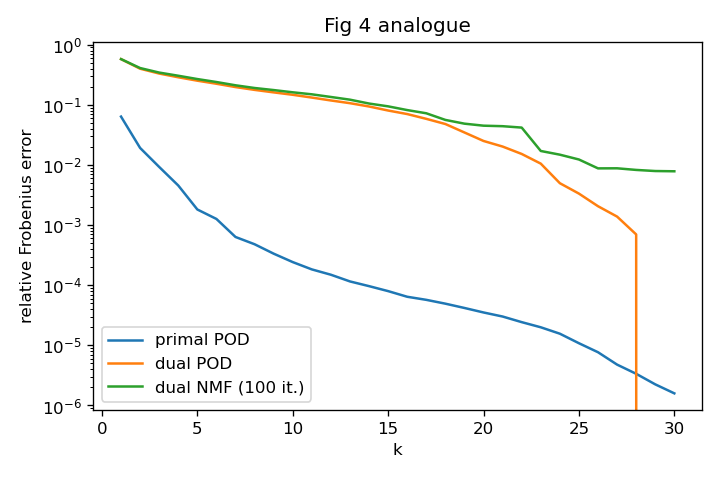
\includegraphics[width=0.7\linewidth]{figures/ch14r/hb_decay.png}
\caption{Best rank-$k$ approximation error of the 120 snapshots: primal POD, dual POD and dual NMF (100 iterations).}\label{fig:vf-hb-decay}
\end{figure}

\emph{Table~1 analogue.} At $\mu=(0.07,0.17)$, which is not in the snapshot set and where the full-order solve takes $1.9$~ms, \Cref{tab:vf-hb-t1} gives the comparison. The accuracy ordering matches the publication (the PB force error is much larger than the hybrid one at comparable displacement accuracy), but the speed-up is not reproduced: the hybrid model has 72 unknowns against 28 and its Lemke solve is slower than the full-order complementarity solve at 100 nodes.

\begin{table}[tbp]
\centering\footnotesize
\caption{Comparison at $\mu=(0.07,0.17)$.}\label{tab:vf-hb-t1}
\begin{tabular}{@{}lrrrr@{}}
\toprule
Model & Unknowns & Speed-up & Displacement error (\%) & Force error (\%)\\
\midrule
HR, $\epsilon_{\rm dual}=0.1$ & 72 & 0.64 (0.36 with reconstruction) & 0.48 & 14.1 on RID / 8.8 reconstructed\\
HR, 1 dual mode & 60 & 1.0 (0.29 with reconstruction) & 0.48 & 14.7 / 16.5\\
PB, $l_u=10$ & 20 & 3.8 & 0.22 & 38.4\\
PB, $l_u=14$ & 28 & 4.2 & 0.037 & 18.8\\
\emph{Publication: HR} & \emph{28} & \emph{8.5 / 5.9} & \emph{0.15} & \emph{13 / 12}\\
\emph{Publication: PB $l_u=9$} & \emph{18} & \emph{8.4} & \emph{0.32} & \emph{44}\\
\emph{Publication: PB $l_u=14$} & \emph{28} & \emph{9.1} & \emph{0.04} & \emph{23}\\
\bottomrule
\end{tabular}
\end{table}

\emph{Solutions and error over the parameter space.} \Cref{fig:vf-hb-sol} shows the displacement and the multipliers: the hybrid displacement cannot be told from the full-order one, the multipliers on the RID lie on the full-order values, and the reconstruction reproduces both contact zones with a slight overshoot at the second peak ($0.035$ against $0.033$); the PB models are accurate in displacement, but their multipliers oscillate and PB 9 overshoots the second peak by about $70\,\%$ ($0.056$ against $0.033$). Over the $100\times120$ test grid (\Cref{fig:vf-hb-errmap}, \Cref{tab:vf-hb-reg}) the displacement error has a mean of $0.74\,\%$ (publication $0.34\,\%$); the force errors are lower than the publication's, which is not a better method but a $2.5$ times larger RID (36 contacts against 14).

\begin{figure}[tbp]
\centering
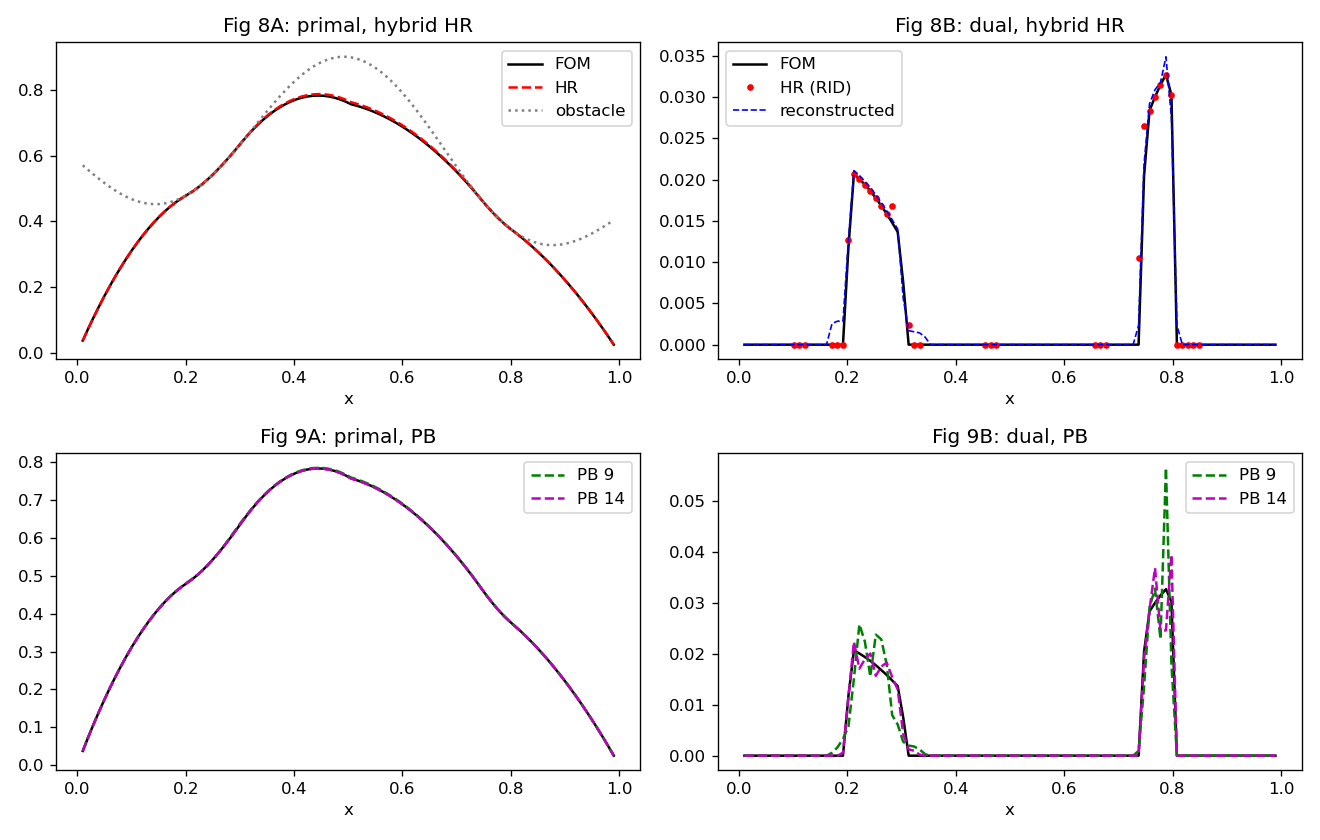
\includegraphics[width=0.95\linewidth]{figures/ch14r/hb_solutions.png}
\caption{Solutions at $\mu=(0.07,0.17)$: displacement (top left), multipliers of the full-order, the hybrid model on the RID and the reconstruction (top right), and the PB models with 9 and 14 modes (bottom).}\label{fig:vf-hb-sol}
\end{figure}

\begin{figure}[tbp]
\centering
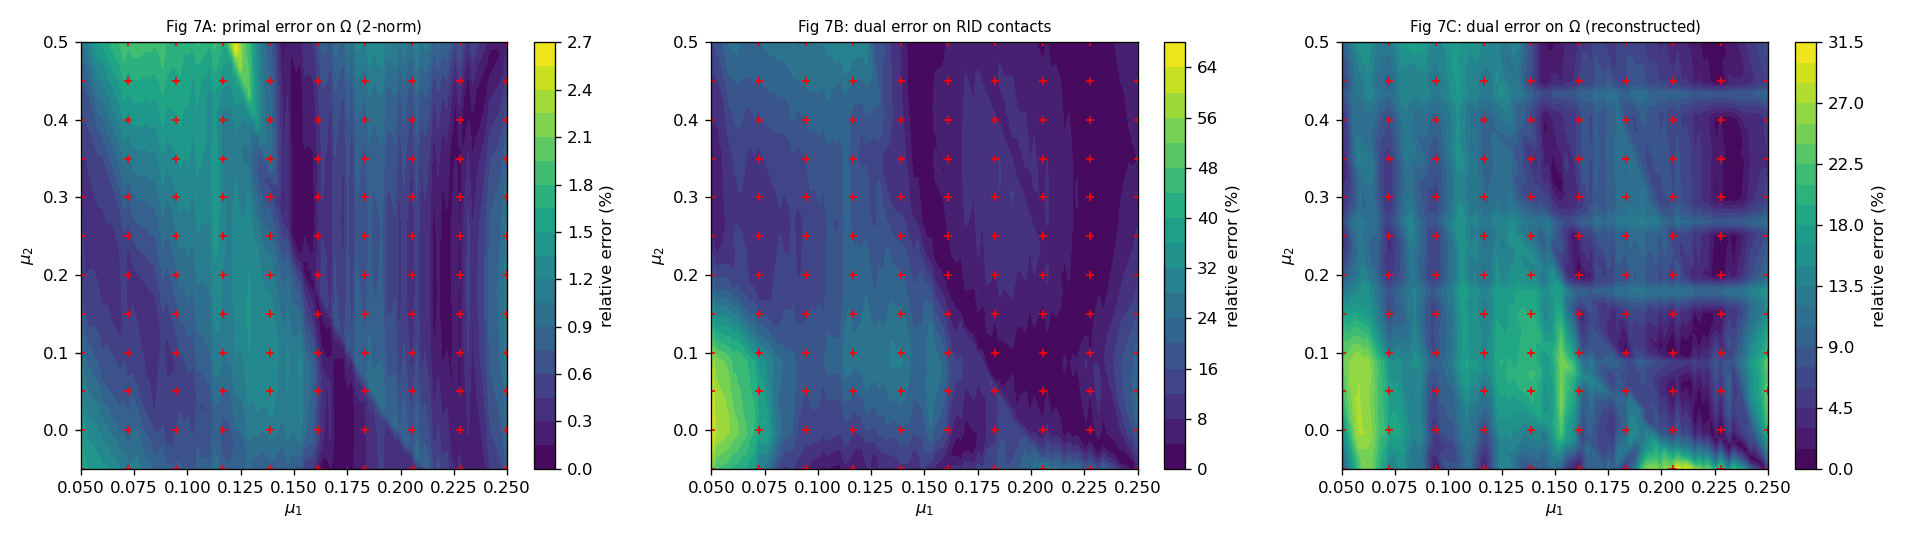
\includegraphics[width=0.98\linewidth]{figures/ch14r/hb_errmap_reg.png}
\caption{Error over the parameter space for the $10\times12$ snapshot grid, $100\times120$ test points: displacement (left), multipliers on the RID (centre), reconstructed multipliers (right); red crosses are the snapshots.}\label{fig:vf-hb-errmap}
\end{figure}

\begin{table}[tbp]
\centering\footnotesize
\caption{Error over the $100\times120$ test grid, regular snapshot grid (12\,000 parameter points, no Lemke failure).}\label{tab:vf-hb-reg}
\begin{tabular}{@{}lrrrr@{}}
\toprule
Quantity & Mean (\%) & Median (\%) & Max (\%) & Publication mean / max (\%)\\
\midrule
Displacement, 2-norm & 0.74 & 0.70 & 2.6 & 0.34 / 1.13\\
Contact force on RID & 13.1 & 10.8 & 66.6 & 24 / 148\\
Contact force over $\Omega$, reconstructed & 10.1 & 9.5 & 31.4 & 39 / 127\\
\bottomrule
\end{tabular}
\end{table}

\subsection*{Results: greedy sampling and the RID size}

With the greedy loop the first run (480 candidates, 50 iterations, $\epsilon_u=10^{-8}$, one element ring, contacts limited to nodes active in some snapshot $\pm1$ node) gives \Cref{fig:vf-hb-greedy1}: the hybrid force error on the RID falls to about $5\,\%$ and the reconstructed one to about $13\,\%$ while PB stays near $55\,\%$, which is the publication's main claim about contact forces; PB wins in the displacement 2-norm ($0.18\,\%$ against $0.49\,\%$) and in the $H^1$ norm the two end close together, so the claim that the hybrid model approximates gradients better is only weakly supported. The displacement accuracy was about $100$ times worse than the publication's ($0.49\,\%$ against $0.004\,\%$ mean).

\begin{figure}[tbp]
\centering
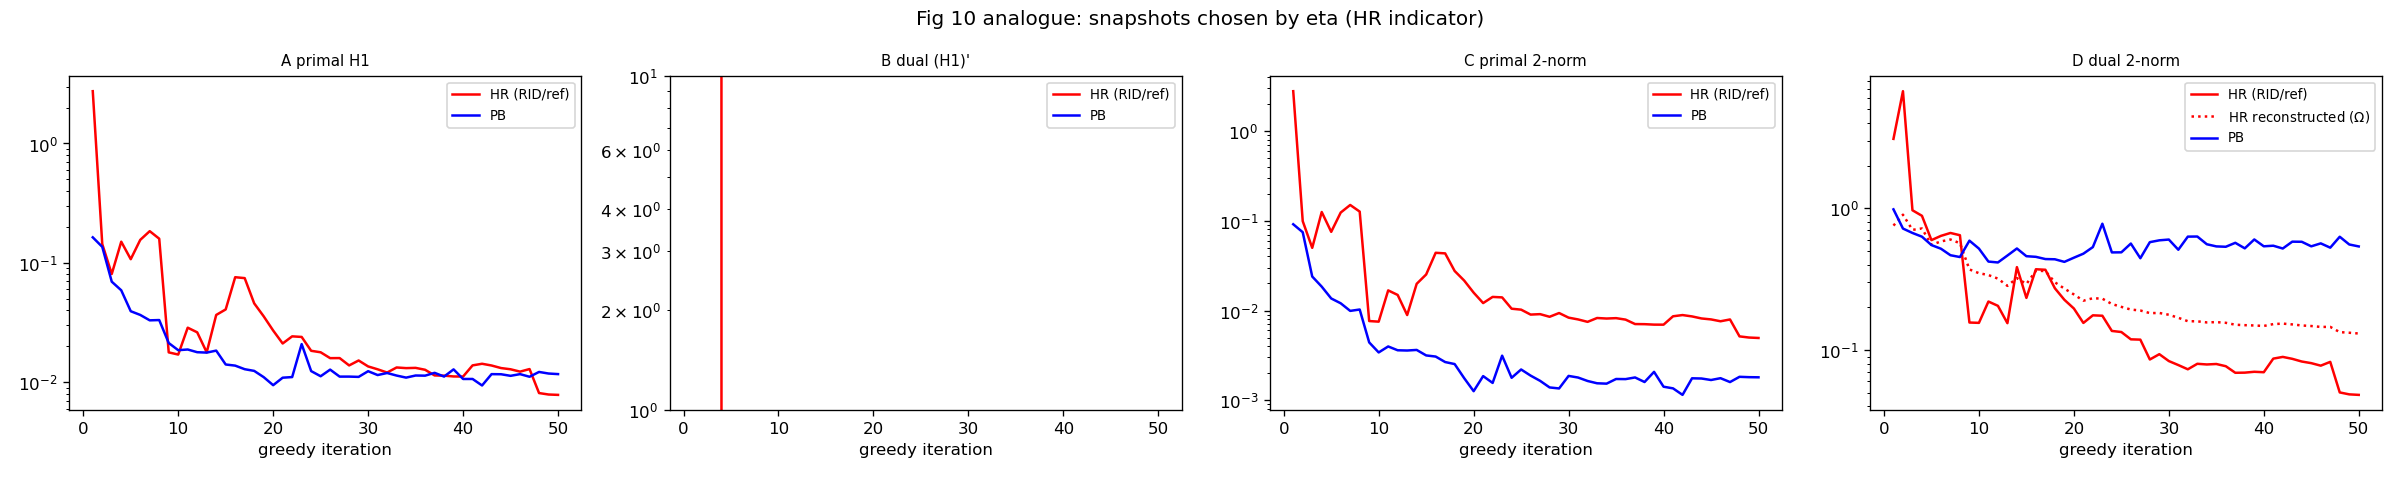
\includegraphics[width=0.95\linewidth]{figures/ch14r/hb_greedy_first.png}
\caption{Greedy loop driven by $\eta$, first run: average error over the 480 candidates for the hybrid (red; dotted: reconstructed multipliers) and PB (blue) models: (A) displacement, $H^1$; (B) multipliers, $(H^1)'$ (not usable in this run); (C) displacement, 2-norm; (D) multipliers, 2-norm.}\label{fig:vf-hb-greedy1}
\end{figure}

\emph{Two failure modes of the reduced system.} Both are properties of the formulation as stated and were diagnosed with scripts in the study. (1) If every node of $\mathcal P$ is a potential contact, the enriched basis has $|\mathcal P|$ columns, so $\mathbf A$ is square; for the $\eta$-selected set $|\mathcal P|=38$ with 38 columns, $\operatorname{cond}(\mathbf A)\approx10^{16}$, smallest singular value $3.7\times10^{-15}$ against $5.8\times10^1$, and the greedy runs gave displacement errors of $5$--$880\,\%$ and one ``good'' run ($0.0016\,\%$) that could not be reproduced. \Cref{tab:vf-hb-sing} lists the remedies tried; the one that works is to keep fewer potential contacts than $|\mathcal P|$, only the nodes that carried a contact force in some snapshot ($\pm1$ node), at the cost that contact outside the snapshot-observed zone is not enforced. (2) At the publication's $\epsilon_u=10^{-10}$ the loop showed spikes (error up to $32\,\%$); the Lemke solve failed on about $35\,\%$ of the parameters because the condensed matrix $\mathbf B_r\mathbf A^{-1}\mathbf B_r^{T}$ is strongly indefinite (minimum eigenvalue of its symmetric part about $-2\max|\text{entry}|$), and with the non-symmetric Petrov--Galerkin system nothing guarantees a well-posed complementarity problem. Alternatives (primal--dual active set, semismooth Newton) flagged $91$--$99\,\%$ of the cases as solved but had median errors of $2.7$--$6.3\,\%$; a symmetric Galerkin form on the RID is always well posed but about $10\,\%$ accurate. Coarsening to $\epsilon_u=10^{-8}$ (max error after iteration 20: $1.6\,\%$, final $0.49\,\%$) was the workaround of the first run.

\begin{table}[tbp]
\centering\footnotesize
\caption{Remedies for the singular reduced matrix ($\eta$-selected snapshots, 160 test parameters).}\label{tab:vf-hb-sing}
\begin{tabular}{@{}lrrrr@{}}
\toprule
Variant & RID nodes & $\operatorname{cond}(\mathbf A)$ & Displacement error median / max (\%) & Lemke failures\\
\midrule
Baseline (primal + dual DEIM, 1 ring) & 38 & $10^{16}$ & 0.36 / 4 & 0\\
+ DEIM on a stress basis & 54 & $2\times10^{16}$ & 6.4 / 73 & 16\\
+ stress DEIM, 2 rings & 72 & $4\times10^{16}$ & 6.4 / 86 & 28\\
+ stress DEIM, 3 rings & 88 of 98 & $6\times10^{3}$ & 0.002 / 0.02 & 0\\
\textbf{Potential contacts limited to ever-active nodes} & 38 & $\mathbf{7\times10^{6}}$ & 1.3 / 12 & 0\\
Same, plus 2 rings & 51 & $2\times10^{6}$ & 2.8 / 102 & 3\\
Unit-vector enrichment without orthogonalisation & 38 & $10^{16}$ & unchanged & ---\\
QR-whitening of the test space & 38 & $2\times10^{15}$ & unchanged & ---\\
Truncated pseudo-inverse of $\mathbf A$ & 38 & --- & about 99 & ---\\
\bottomrule
\end{tabular}
\end{table}

\emph{The remaining gap was the RID size.} A chain of negative results ruled out the other causes: the POD size (the Petrov--Galerkin system is square after enrichment, so the contact rows and not $l_u$ fix the accuracy), the dual mode count and the RID thickness at paper size, the indefiniteness of the complementarity matrix (a symmetric least-squares active-set solve was worse, $2.0\,\%$ mean, and giving it the exact full-order contact set still left $0.56$--$0.75\,\%$ error), the snapshot set (greedy snapshots were no better than 50 random ones) and the load sign (an exact mirror). Projecting the full-order solution on the enriched basis gives $0.004\,\%$ error, the publication's figure, while the hybrid solve gives $0.67\,\%$, so the basis was not the limit; the error enters when the displacements on $\mathcal P$ are tied to $\mathbf V\boldsymbol\gamma$, and the hybrid solve is no more accurate than interpolating the snapshot coefficients with no RID solve ($0.78\,\%$). What decides it is how much of the domain the RID covers (\Cref{fig:vf-hb-rid}): for 50 random snapshots a RID of 37 nodes gives $0.6\,\%$, 89 nodes $0.012\,\%$ (and $3\times10^{-4}\,\%$ with every RID node a contact and $\epsilon_u=10^{-10}$), 98 nodes exact; the dependence is not monotone below about 66 nodes, so a few extra rings are not enough unless the RID is large. The publication gives no final RID size.

\begin{figure}[tbp]
\centering
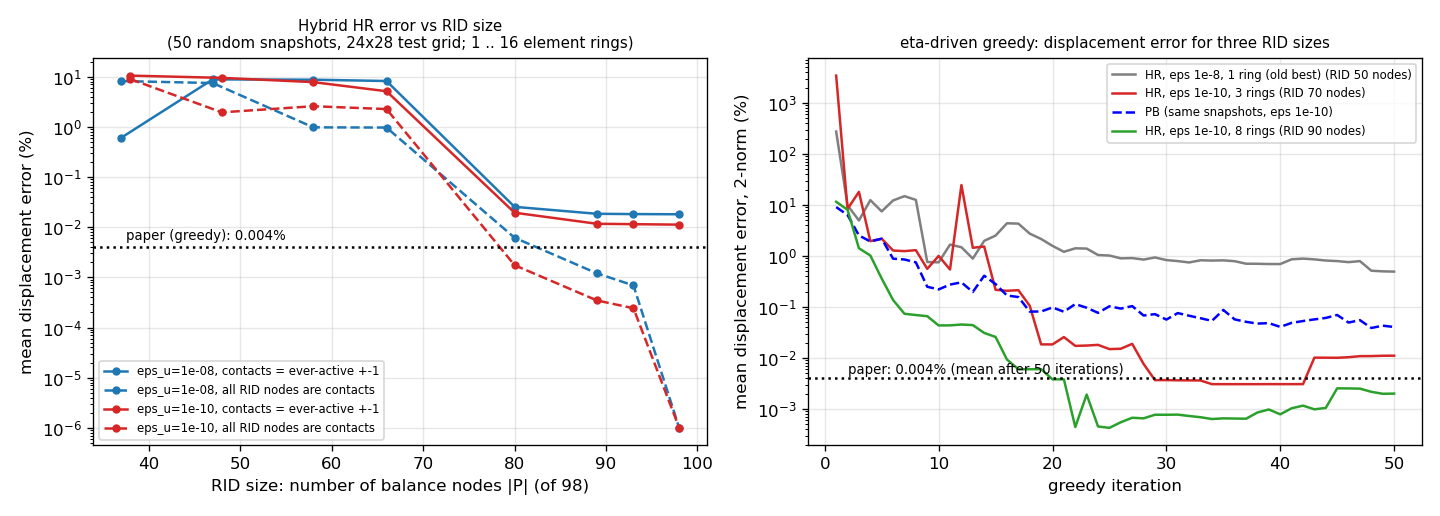
\includegraphics[width=0.98\linewidth]{figures/ch14r/hb_rid.png}
\caption{The RID size sets the accuracy. Left: mean displacement error of the hybrid model against the number of balance nodes $|\mathcal P|$ for RIDs grown by 1--16 rings, two POD tolerances and two contact sets; the dotted line is the publication's greedy accuracy. Right: mean error over the candidate set at each greedy iteration for three RID sizes; the blue dashed line is PB on the same snapshots.}\label{fig:vf-hb-rid}
\end{figure}

\Cref{tab:vf-hb-greedy} gives the greedy runs. With a large RID the $\epsilon_u=10^{-10}$ setting no longer needs the workaround, and the run `$\_$L3e10' (three rings, 70 nodes) is the closest match to the publication in all displacement and RID-force numbers (\Cref{fig:vf-hb-greedy2,fig:vf-hb-errmap2}); once the RID is large the hybrid model is 4 to 20 times more accurate than PB in displacement, and the larger RID also means no cost reduction on this 100-node mesh.

\begin{table}[tbp]
\centering\footnotesize
\setlength{\tabcolsep}{3pt}
\caption{Greedy runs (50 iterations, $\eta$-driven, 20$\times$24 candidates, $50\times60$ test grid).}\label{tab:vf-hb-greedy}
\begin{tabular}{@{}lrrrrrrr@{}}
\toprule
Run & $\epsilon_u$ & Rings & RID nodes & Unknowns & Displacement mean / max & Force on RID mean / max & Reconstructed mean / max\\
\midrule
first (\texttt{\_L1}) & $10^{-8}$ & 1 & 50 & 60 & 0.49\,\% / 3.1\,\% & 4.7\,\% / 66\,\% & 13\,\% / 66\,\%\\
\texttt{\_L8} & $10^{-8}$ & 8 & 90 & 66 & 0.025\,\% / 0.11\,\% & 12.6\,\% / 49.9\,\% & 14.4\,\% / 45.4\,\%\\
\texttt{\_L8e10} & $10^{-10}$ & 8 & 90 & 66 & 0.0021\,\% / 0.019\,\% & 0.25\,\% / 2.0\,\% & 8.0\,\% / 45.3\,\%\\
\texttt{\_L3e10} & $10^{-10}$ & 3 & 70 & 66 & 0.011\,\% / 0.084\,\% & 0.45\,\% / 9.6\,\% & 10.3\,\% / 36.1\,\%\\
Publication & $10^{-10}$ & --- & n/a & n/a & 0.004\,\% / 0.077\,\% & 0.34\,\% / 10\,\% & 1.3\,\% / 18\,\%\\
\bottomrule
\end{tabular}
\end{table}

\begin{figure}[tbp]
\centering
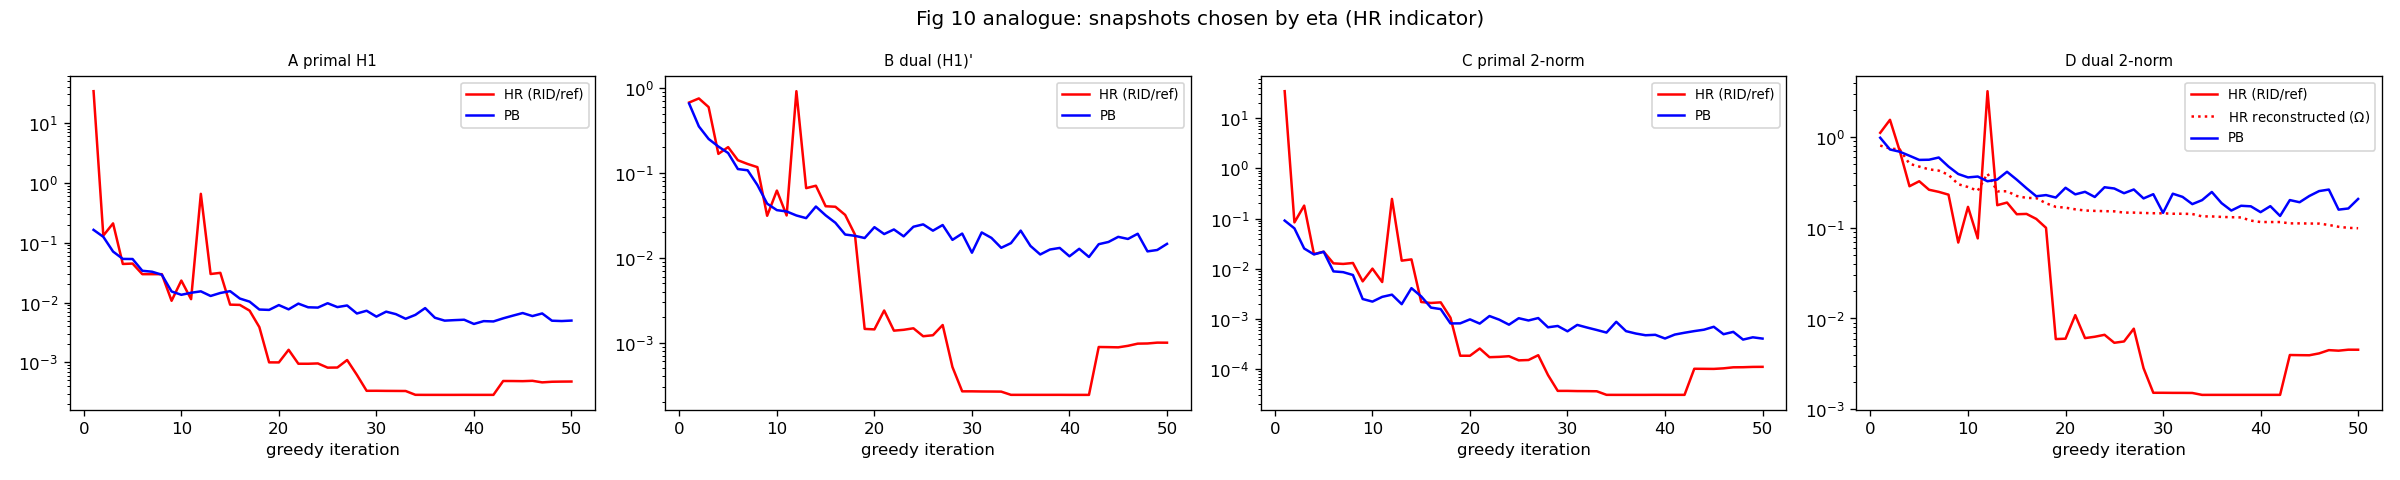
\includegraphics[width=0.95\linewidth]{figures/ch14r/hb_greedy_best.png}
\caption{Greedy loop driven by $\eta$, best run (3 rings, $\epsilon_u=10^{-10}$, 70 RID nodes), panels as in \Cref{fig:vf-hb-greedy1}. The hybrid displacement error falls to $3$--$5\times10^{-4}$ in the $H^1$ norm against $5\times10^{-3}$ for PB, with one spike at iteration 12 (a bad reduced complementarity solve).}\label{fig:vf-hb-greedy2}
\end{figure}

\begin{figure}[tbp]
\centering
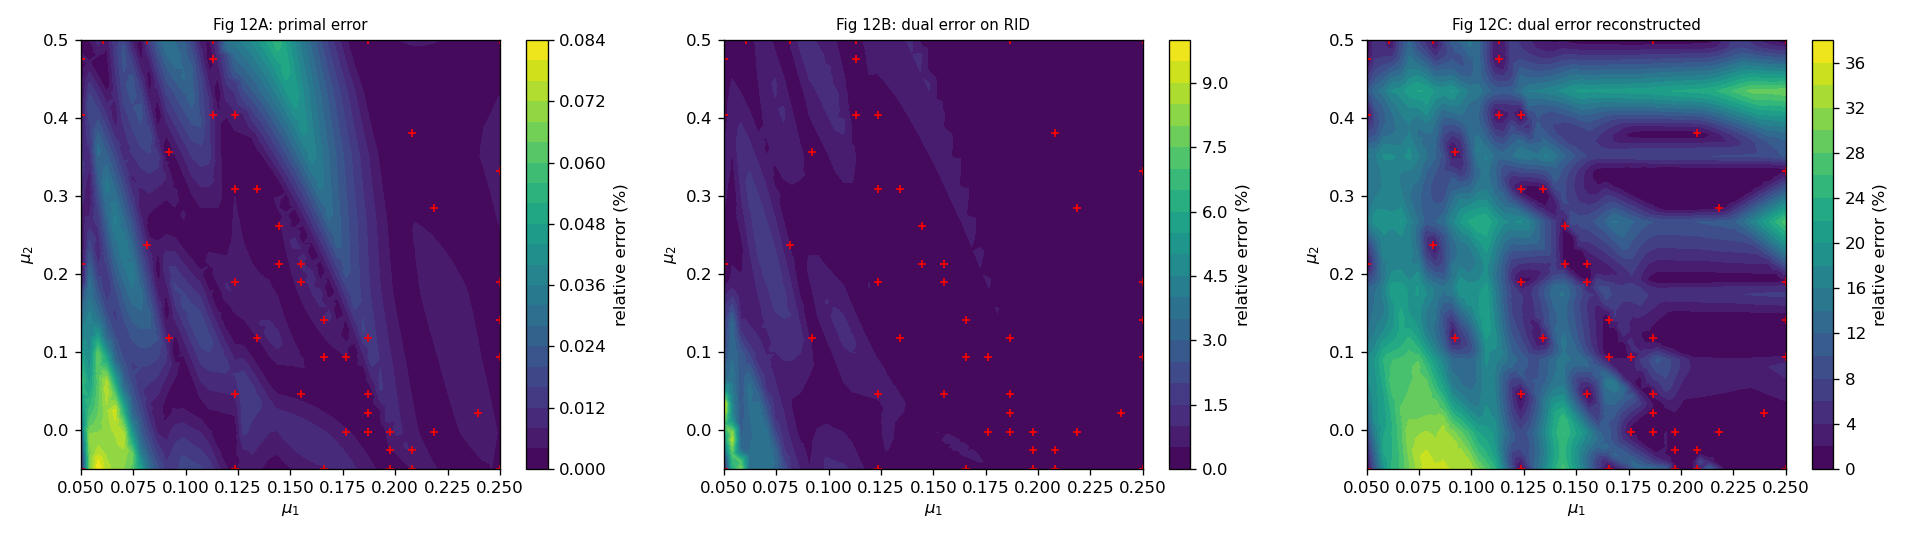
\includegraphics[width=0.95\linewidth]{figures/ch14r/hb_errmap_best.png}
\caption{Error maps after the greedy loop, best run, $100\times120$ test points: displacement (mean $0.011\,\%$, maximum $0.084\,\%$), multipliers on the RID (maximum about $10\,\%$) and reconstructed multipliers (maximum about $38\,\%$); highest at small $\mu_1$, where the contact zone is largest.}\label{fig:vf-hb-errmap2}
\end{figure}

\begin{figure}[tbp]
\centering
\includegraphics[width=1.0\linewidth]{figures/ch14_hyb.pdf}
\caption{Greedy loop for the rope problem of \citet{fauque2018hybrid}, best run. (a), (b) Error of the hybrid (HR, hyper-reduced) and projection-based (PB) reduced models against the iteration (displacement mean \cvfHybDispMean{}, maximum \cvfHybDispMax{}; contact force on the reduced domain \cvfHybForceMean{} mean, reconstructed force \cvfHybForceRecon{} mean at the end). (c) Size of the reduced problem.}\label{fig:vf-hyb}
\end{figure}

\subsection*{Geometry and mesh: the three-dimensional pellet--cladding problem}

One eighth of the problem is modelled, a $90^\circ$ sector and half the height, with symmetry planes $x=0$, $y=0$, $z=0$ (\Cref{fig:vf-hb3-geom}). The pellet has radius $R_p\le R_p^{\max}$, the cladding spans $4.1\le r\le4.7$~mm, and the half height is $6.75$~mm (the publication's pellet is 13.5~mm). The simulations S1--S5 differ only in the pellet radius: S1 $R_p=4.10$ (no gap), S2 $4.02$, S3 $4.06$, S4 $4.04$, S5 $4.08$. The loads are $5$~MPa axial on the pellet top and a radial pressure on the cladding outside of $250$~MPa for $z<2$~mm and $50$~MPa above, applied in 25 steps by a linear ramp. The material is $E=10^5$~MPa and $\nu=0.3$ for both bodies; the publication prints ``105 MPa'', which is read as $10^5$~MPa because with it the cladding closes by about $0.08$~mm at full load, which matches the gaps chosen in the publication. The mesh is a structured hexahedral mesh in $(r,\theta,z)$, pellet $6\times8\times27$ and cladding $3\times8\times27$ elements: 1944 elements, 2548 nodes, 6937 free degrees of freedom, with 252 node-to-node contact pairs on matching meshes and the axis nodes shared (collapsed hexahedra). The contact is frictionless and small-displacement with a gap along $\mathbf e_r$, $(\mathbf u_{\rm pellet}-\mathbf u_{\rm clad})\cdot\mathbf e_r\le4.1-R_p$, solved with the active-set solver of \fea{}. The RID is the union of the sets of displacement, stress and generalised-force modes (generalised forces being $\mathbf K\mathbf u$ over all degrees of freedom) and a region of interest (the top layer of the pellet and two element rings next to the axis, 16 elements; the publication does not specify it), extended by the contact-surface distance $d=0.1$~mm and one layer of elements.

\begin{figure}[tbp]
\centering
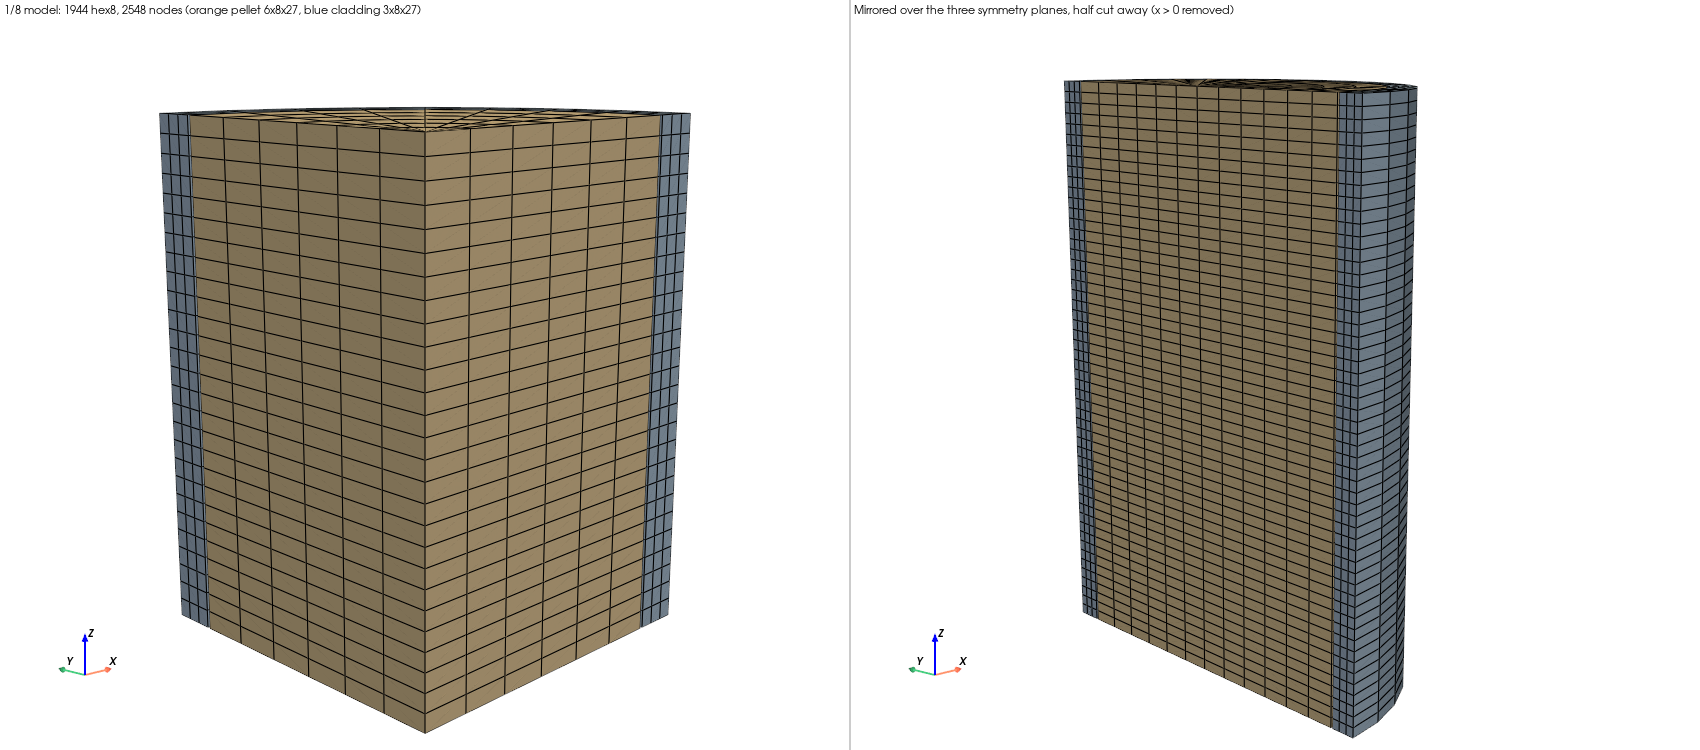
\includegraphics[width=0.95\linewidth]{figures/ch14r/hb3_geom.png}
\caption{Pellet--cladding model: the one-eighth model (pellet orange, cladding blue, case S3) and the same mesh mirrored over the symmetry planes with one half cut away.}\label{fig:vf-hb3-geom}
\end{figure}

\emph{Validation of the finite element model.} Rigid translations lie in the null space of the unconstrained stiffness (residual $10^{-15}$); the Lam\'e thick cylinder under external pressure, with three elements through the thickness, gives inner and outer radial displacements within $0.25\,\%$ and $0.23\,\%$ of the closed form (angular spread $2\times10^{-14}$); and pellet uniaxial compression gives the exact top displacement and $\sigma_{zz}=-5$~MPa in every element. An earlier version used the transposed Jacobian inverse (errors of $17$--$69\,\%$ in the Lam\'e test), fixed and verified by these checks. The full-order behaviour: S1 has all 252 pairs in contact from step 1; S2 first touches at step 25 (18 pairs); S3 at step about 12 (63 pairs at the end); S4 at about step 16 (36 pairs); S5 at about step 6 (90 pairs). \Cref{fig:vf-hb3-fom} shows the stresses of S3: the cladding is pressed in by up to $0.044$~mm where the 250~MPa pressure acts and has closed the gap there, its hoop stress reaches about $-1000$~MPa (von Mises up to $1062$~MPa) while the pellet stays below about $250$~MPa, with a stress concentration at the end of the contact zone ($z\approx1.5$--$2$~mm).

\begin{figure}[tbp]
\centering
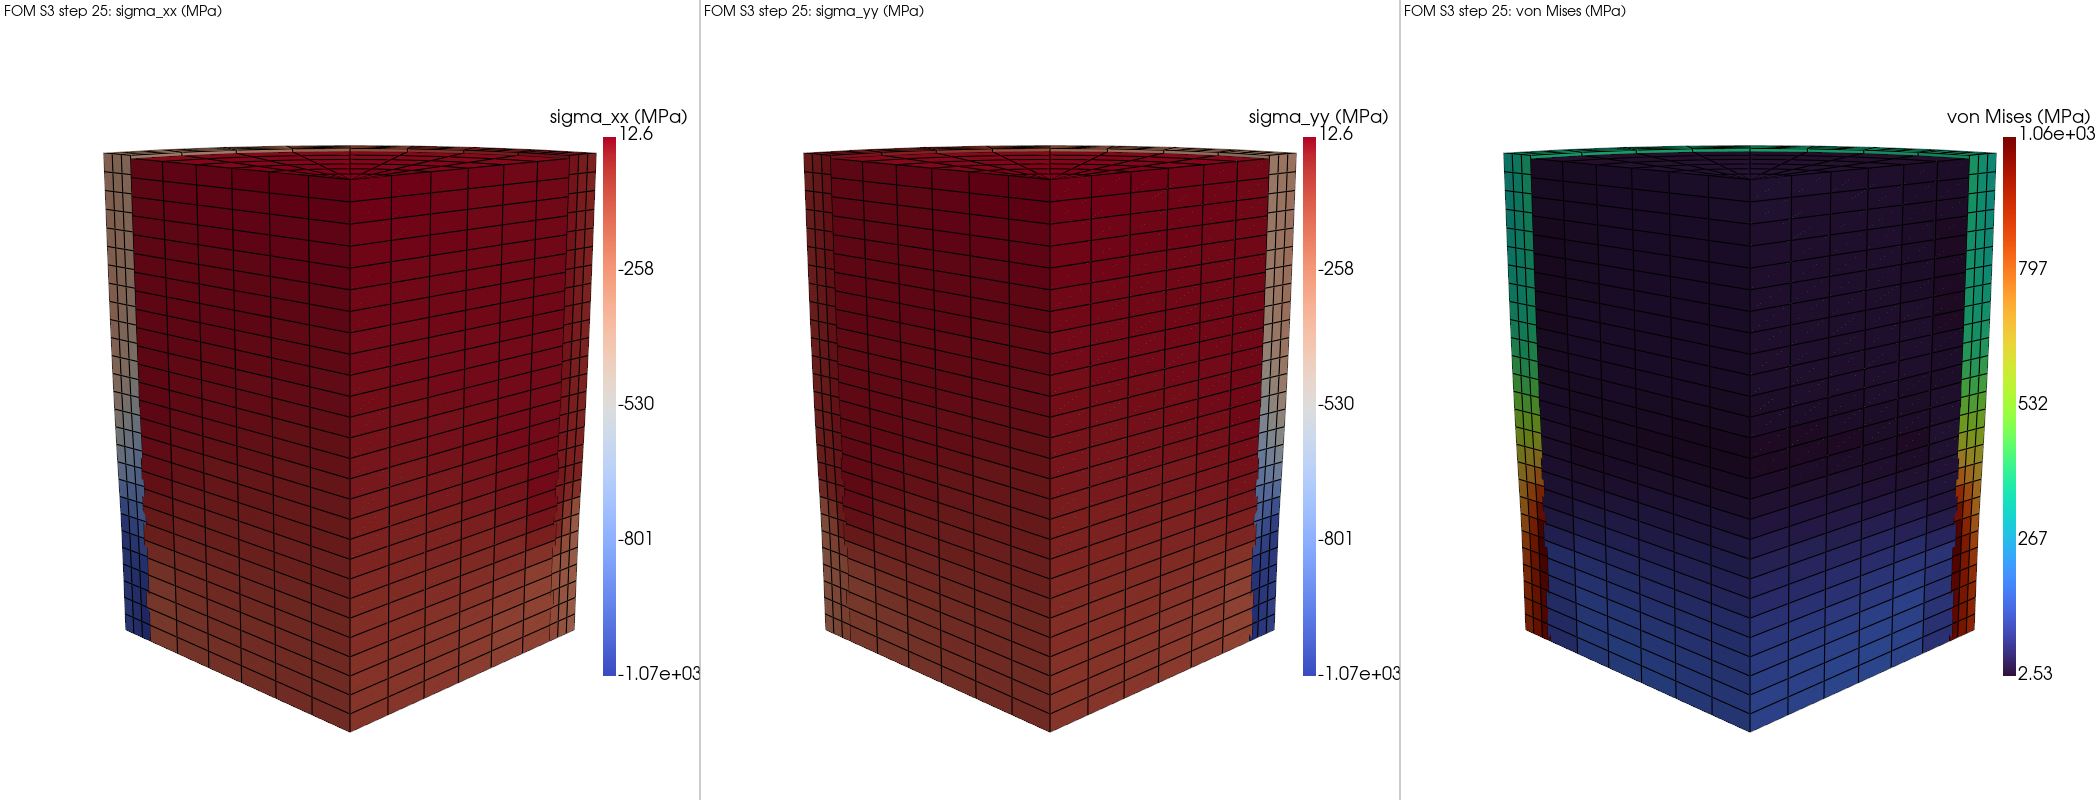
\includegraphics[width=0.95\linewidth]{figures/ch14r/hb3_fom.png}
\caption{Full-order solution of S3 at step 25 (deformation magnified three times, element-centroid values): $\sigma_{xx}$, $\sigma_{yy}$ and von Mises stress seen from the symmetry planes.}\label{fig:vf-hb3-fom}
\end{figure}

\subsection*{Results: prediction of S3 from snapshots}

The error of the displacement is the maximum over RID degrees of freedom of $|\mathbf u_{HR}-\mathbf u_{FOM}|/\max|\mathbf u_{FOM}|$ at the worst step, that of the stress the same for $\sigma_{11}$ over RID elements, and ``agree'' is the fraction of RID contact pairs whose active or inactive state matches the full-order one at the worst step (publication: displacement $1\,\%$, stress $5\,\%$, speed-up $10$). \Cref{tab:vf-hb3-cases} and \Cref{fig:vf-hb3-err} give the cases. With the publication's training set (S1 and S2, case A) the error reaches $13$--$19\,\%$ in displacement; adding two simulations with intermediate gaps (S4, S5, case B, which interpolates in the gap and never uses S3) reduces it to $0.05\,\%$ in displacement and $0.21\,\%$ in stress with a correct contact set at every step (B2), better than the publication's limits. Before contact starts (steps 1--11) all cases are accurate to $0.26\,\%$ or better, and the error of every case changes at contact onset (step 12). Timings come from single runs and vary by about $\pm20\,\%$.

\begin{table}[tbp]
\centering\footnotesize
\setlength{\tabcolsep}{3pt}
\caption{Prediction of S3 (25 steps). Modes u/s/F: displacement, stress, generalised-force modes.}\label{tab:vf-hb3-cases}
\begin{tabular}{@{}llrrrrrrrr@{}}
\toprule
Case & Training & POD tol. & Modes u/s/F & RID elements & Contact pairs & Disp. & Stress & Agree & Speed-up\\
\midrule
A1 & S1+S2 (publication), minimal enrichment & $10^{-5}$ & 3/3/3 & 12\,\% & 42 & 19.3\,\% & 8.8\,\% & 71\,\% & 9.6$\times$\\
A2 & S1+S2, full FE contact dofs, 2 layers & $10^{-11}$ & 4/4/4 & 26\,\% & 73 & 13.4\,\% & 10.0\,\% & 88\,\% & 5.7$\times$\\
B1 & S1+S2+S4+S5, full FE contact dofs & $10^{-5}$ & 4/6/11 & 29\,\% & 130 & 3.35\,\% & 4.04\,\% & 93\,\% & 4.0$\times$\\
\textbf{B2} & same, 1 layer & $10^{-8}$ & 9/12/12 & 32\,\% & 142 & \textbf{0.050\,\%} & \textbf{0.21\,\%} & 100\,\% & 3.7$\times$\\
B3 & same, 1 layer & $10^{-11}$ & 13/14/15 & 33\,\% & 148 & 0.055\,\% & 0.055\,\% & 100\,\% & 3.5$\times$\\
B4 & same, 2 layers & $10^{-11}$ & 13/14/15 & 59\,\% & 190 & 0.010\,\% & 0.017\,\% & 100\,\% & 2.1$\times$\\
Publication & S1+S2 & $10^{-5}$ & 17/20/21 & --- & --- & 1\,\% & 5\,\% & --- & 10$\times$\\
\bottomrule
\end{tabular}
\end{table}

\begin{figure}[tbp]
\centering
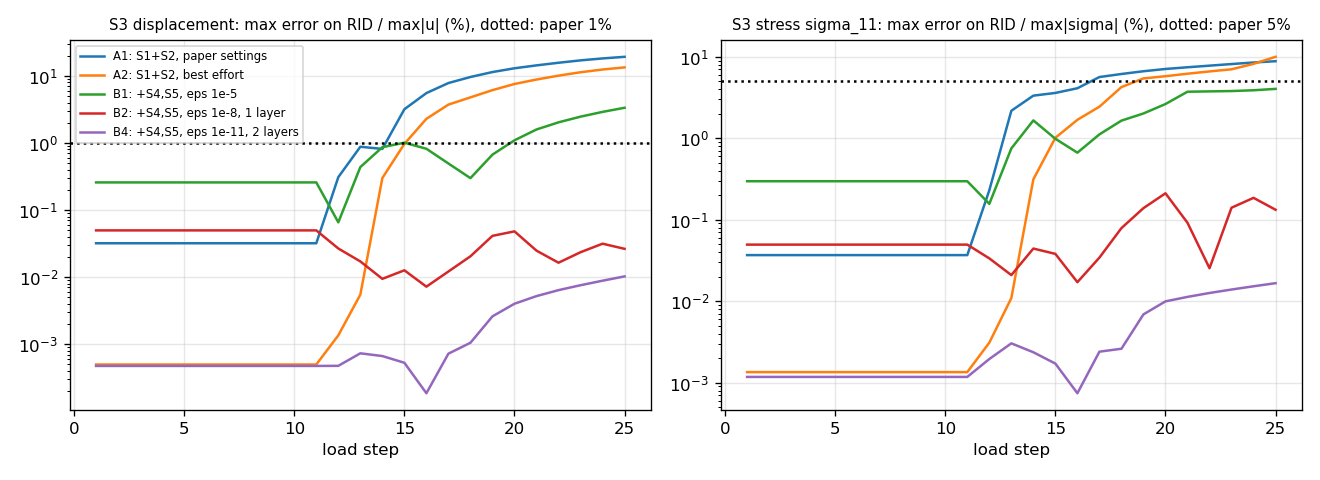
\includegraphics[width=0.95\linewidth]{figures/ch14r/hb3_errors.png}
\caption{Prediction error of S3 at each load step for cases A1--B4: displacement (left) and $\sigma_{11}$ (right), maximum over the RID relative to the maximum value; dotted lines are the publication's $1\,\%$ and $5\,\%$.}\label{fig:vf-hb3-err}
\end{figure}

\emph{Why the publication's training set is not enough here.} The 50 snapshots of S1 and S2 have normalised singular values $1$, $0.11$, $5.6\times10^{-3}$, $5.2\times10^{-5}$ and then $10^{-15}$: rank 4. S1 is bonded and exactly linear in the load, and S2 is free until the last step. A POD tolerance of $10^{-5}$ gives 3 modes, not the publication's 17, and the four-mode basis alone has a $6\,\%$ projection error on the last step of S3 (\Cref{fig:vf-hb3-rank}); S3's contact reaction is up to $61\,\%$ of its solution but only one S2 step (18 pairs) shows contact in the training data. The publication's 17, 20 and 21 modes mean its S1 and S2 snapshots contained much richer contact evolution; why could not be recovered. Adding S4 and S5 gives a slowly decaying spectrum and 9 modes at tolerance $10^{-8}$, with the projection error of S3 below $5\times10^{-4}$ at every step. A second finding is that keeping every primal degree of freedom of the potential contact zone as a finite element degree of freedom (the publication's Sec.~7.3) is essential: with the minimal rank-completing enrichment of the rope case and the same training data the error is $13.7\,\%$ against $3.35\,\%$ (B1).

\begin{figure}[tbp]
\centering
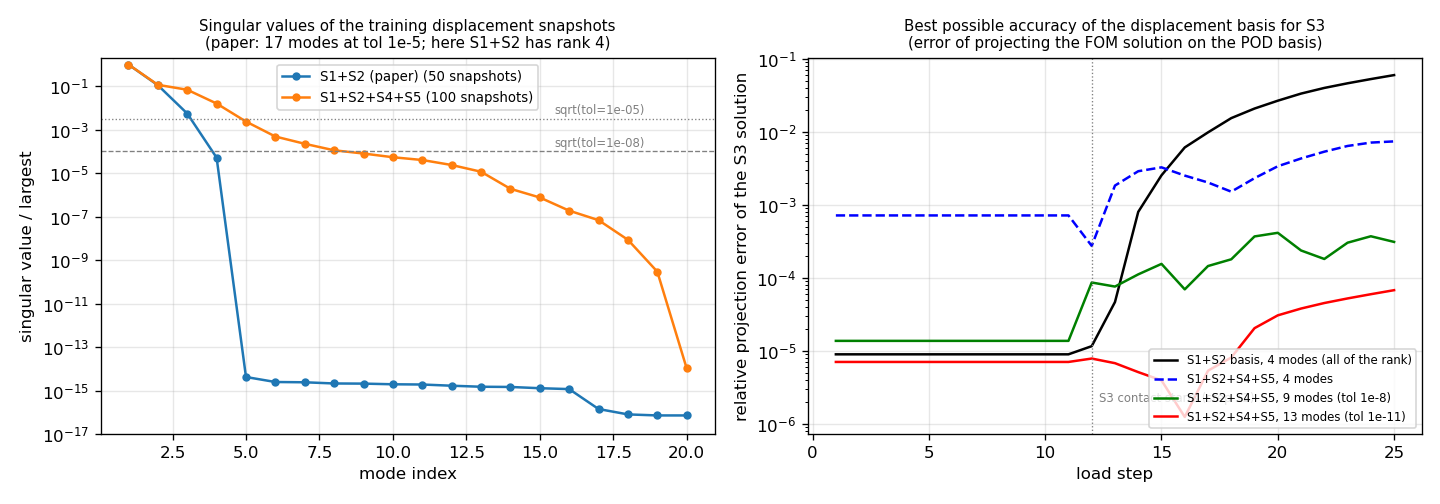
\includegraphics[width=0.95\linewidth]{figures/ch14r/hb3_rank.png}
\caption{Left: singular values of the displacement snapshots for S1+S2 (50 snapshots, exactly four non-negligible values) and S1+S2+S4+S5 (100). Right: projection error of the full-order S3 solution on the basis, the best any model built on it can do.}\label{fig:vf-hb3-rank}
\end{figure}

\emph{Fields, RID and contact.} \Cref{fig:vf-hb3-hrom} compares the von Mises stress of the full model and of case B2 on the whole body: the fields are visually identical and the largest difference is $1.05$~MPa against a peak of $1062$~MPa ($0.10\,\%$); the displacement magnitude differs by a relative $L^2$ error of $4.0\times10^{-4}$. \Cref{fig:vf-hb3-rid} shows the RID, 616 of 1944 elements ($32\,\%$), and the contact force per pair, active only below $z=2$~mm. The contact behaviour of S1--S3 is in \Cref{fig:vf-hb3-contact}: S1 is in contact everywhere with the largest forces below $z=2$~mm, S2 has only just touched (18 pairs), S3 has 63 active pairs for $z<1.5$~mm, which is why S1 and S2 alone teach the basis almost nothing about partial contact; the loaded zone grows upwards with the load, the peak is about 16~N per pair, and the cladding moves in by about 44~\textmu m at the bottom while the pellet moves about 4~\textmu m, so the difference of 40~\textmu m equals the initial gap where the surfaces touch; the HROM markers lie on the full-order curves.

\begin{figure}[tbp]
\centering
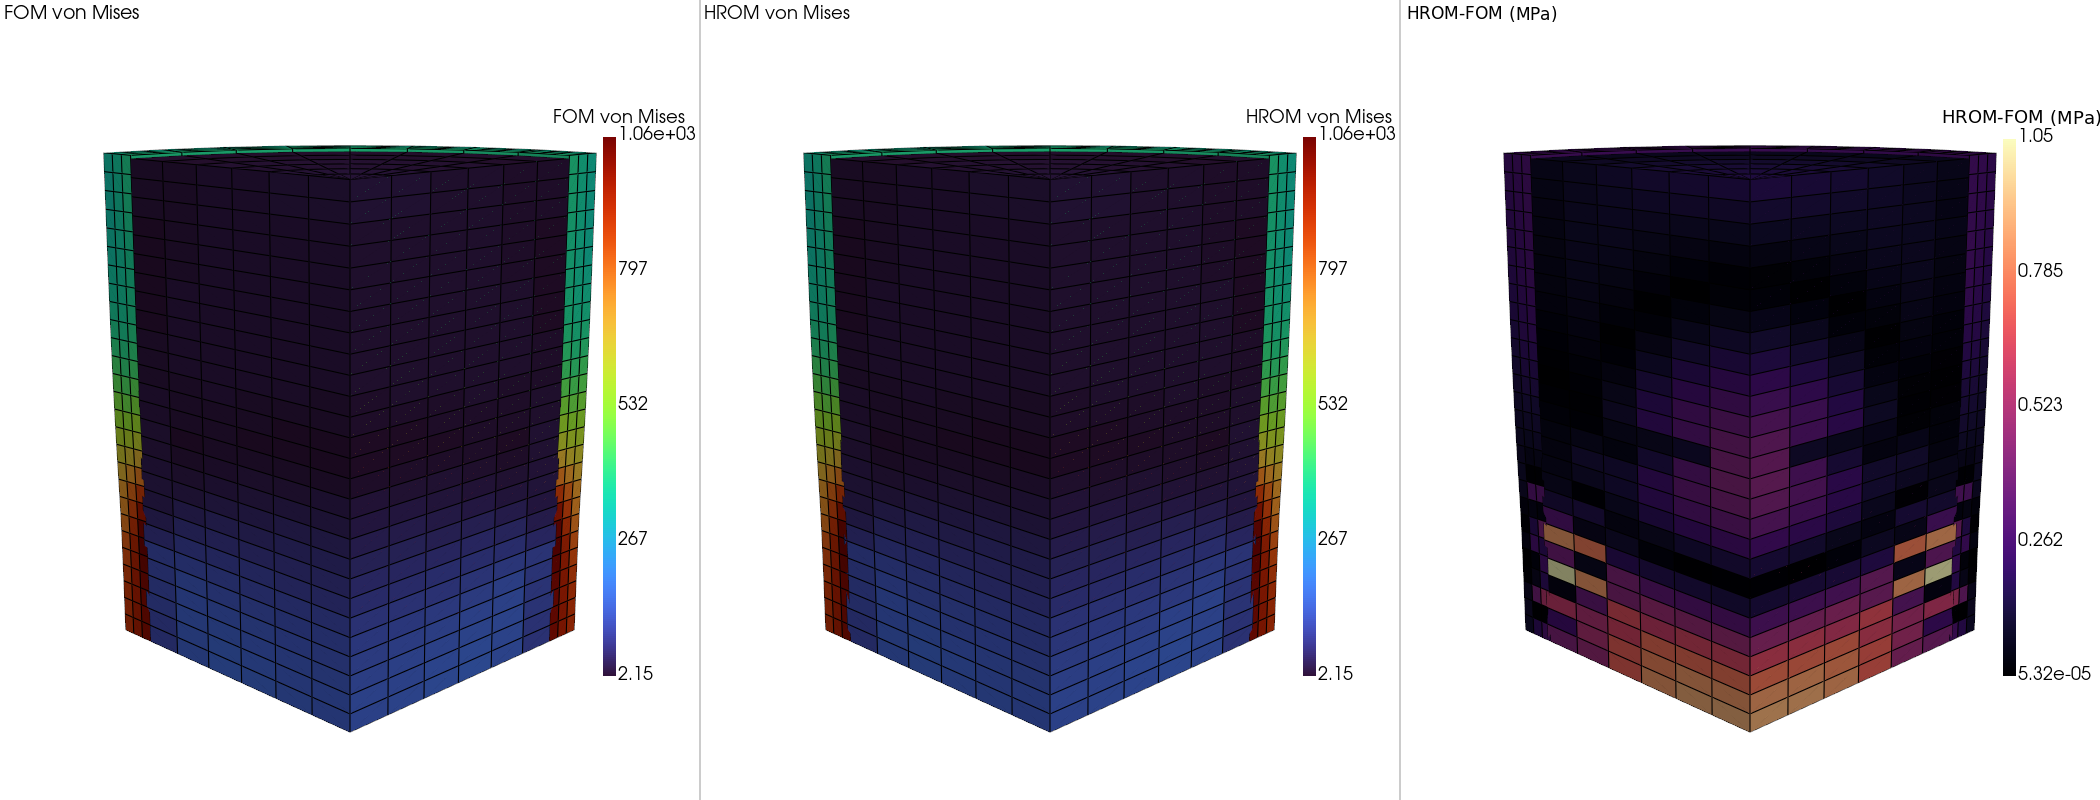
\includegraphics[width=0.98\linewidth]{figures/ch14r/hb3_hrom.png}
\caption{Hybrid HROM against the full model for S3 at step 25 (case B2): von Mises stress from the full model, from the HROM reconstructed on the whole body, and their absolute difference.}\label{fig:vf-hb3-hrom}
\end{figure}

\begin{figure}[tbp]
\centering
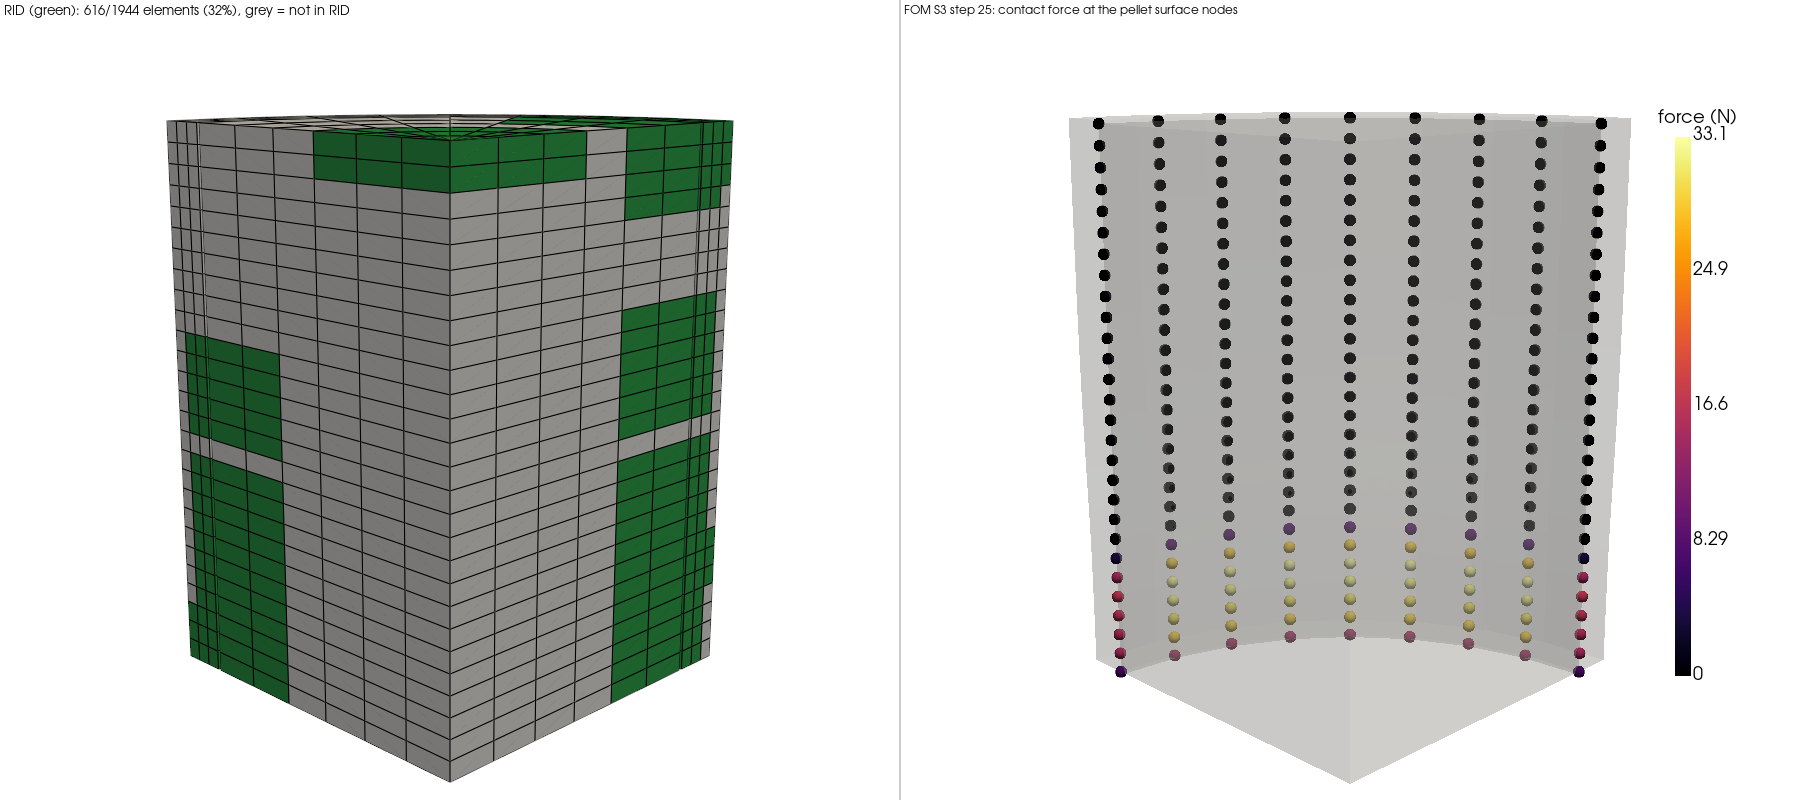
\includegraphics[width=0.95\linewidth]{figures/ch14r/hb3_rid.png}
\caption{Left: the RID (616 of 1944 elements, green). Right: contact force per pair on the pellet surface nodes at step 25.}\label{fig:vf-hb3-rid}
\end{figure}

\begin{figure}[tbp]
\centering
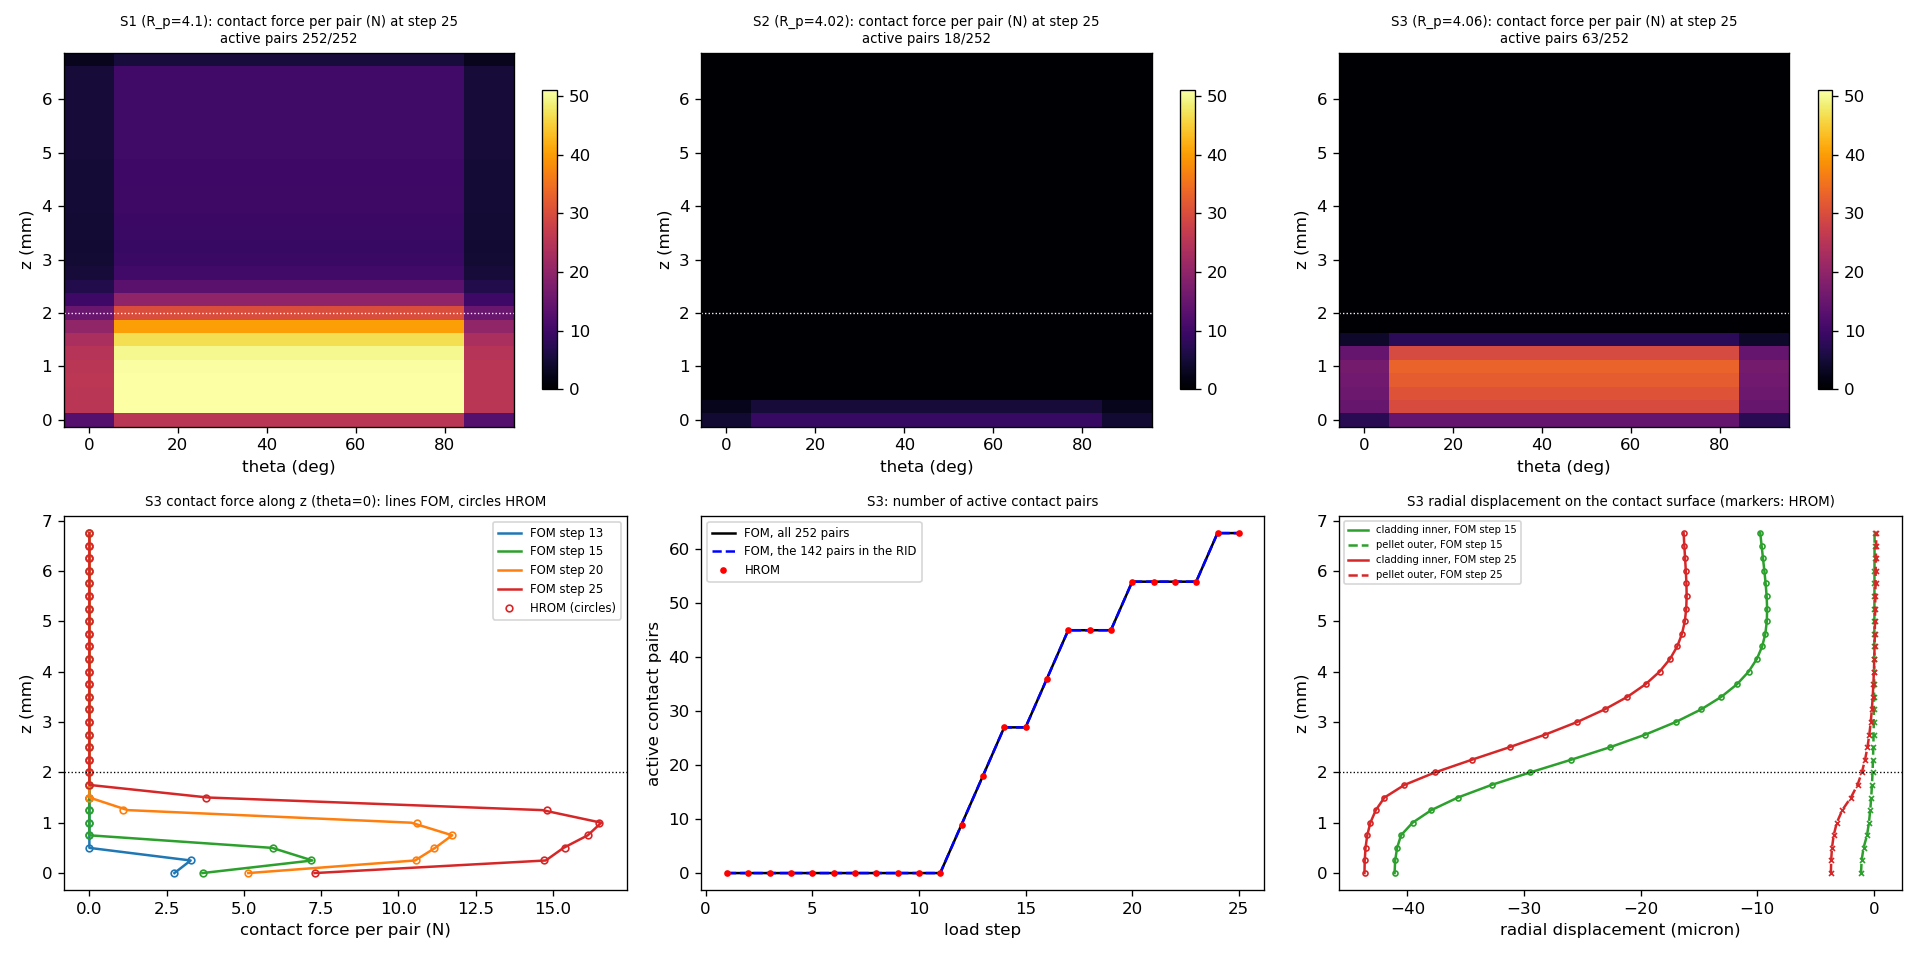
\includegraphics[width=0.98\linewidth]{figures/ch14r/hb3_contact.png}
\caption{Contact behaviour: contact force per pair over the contact surface for S1, S2, S3 (top); S3 contact force along $z$ at several steps, number of active pairs per step for the full model, the restricted count and the HROM, and radial displacements of the cladding inner surface and of the pellet outer surface (bottom).}\label{fig:vf-hb3-contact}
\end{figure}

\subsection*{Results: mesh refinement, RID size and extrapolation (3D)}

The case B2 model was run on meshes refined in all directions (\Cref{tab:vf-hb3-mesh}, \Cref{fig:vf-hb3-mesh}). The full-order time grows about 24 times for 7.3 times more degrees of freedom (sparse LU and the dense Delassus matrix with one column per contact pair), while the HROM time grows only 1.5 times, because the RID barely grows (616 to 914 elements); the speed-up therefore rises from $3.2$ to $11$ to $50$, and the publication's $10\times$ is crossed between the first two meshes. The low speed-up of the baseline is a consequence of the small mesh and not of the method, but the speed-up at the publication's mesh size cannot be stated because its mesh size is not given. Accuracy stays inside the publication's limits on all three meshes (displacement below $0.23\,\%$, $\sigma_{11}$ below $1.3\,\%$), a factor of 4 to 6 larger than on the baseline, and the contact-force error rises from $1.9\,\%$ to $7$--$8\,\%$. A caveat is that on the refined meshes the RID rows contain only 104 of the 221 contact pairs active for S3 at the last step, and the contact-set agreement inside the RID drops to $95.8\,\%$; the pairs outside the RID are not enforced, yet the errors stay small, and where those pairs lie was not examined. The offline time grows from 19~s to 140~s.

\begin{table}[tbp]
\centering\footnotesize
\setlength{\tabcolsep}{3pt}
\caption{Mesh study (case B2; S3 prediction). Meshes: elements per direction (pellet radial, cladding radial, circumferential, axial).}\label{tab:vf-hb3-mesh}
\begin{tabular}{@{}lrrrrrrrr@{}}
\toprule
Mesh & Elements & Free dofs & Contact pairs & RID elements & FOM time (s) & HROM time (s) & Speed-up & Worst $u$ / $\sigma_{11}$ / force error\\
\midrule
L1 (6, 3, 8, 27) & 1944 & 6937 & 252 & 616 (31.7\,\%) & 5.6 & 1.76 & 3.2$\times$ & 0.050 / 0.21 / 1.9\,\%\\
L1.5 (9, 5, 12, 40) & 6720 & 22\,600 & 533 & 860 (12.8\,\%) & 23.2 & 2.10 & 11.0$\times$ & 0.18 / 1.21 / 7.5\,\%\\
L2 (12, 6, 16, 54) & 15\,552 & 50\,936 & 935 & 914 (5.9\,\%) & 134.9 & 2.71 & 49.7$\times$ & 0.23 / 1.27 / 8.4\,\%\\
\bottomrule
\end{tabular}
\end{table}

\begin{figure}[tbp]
\centering
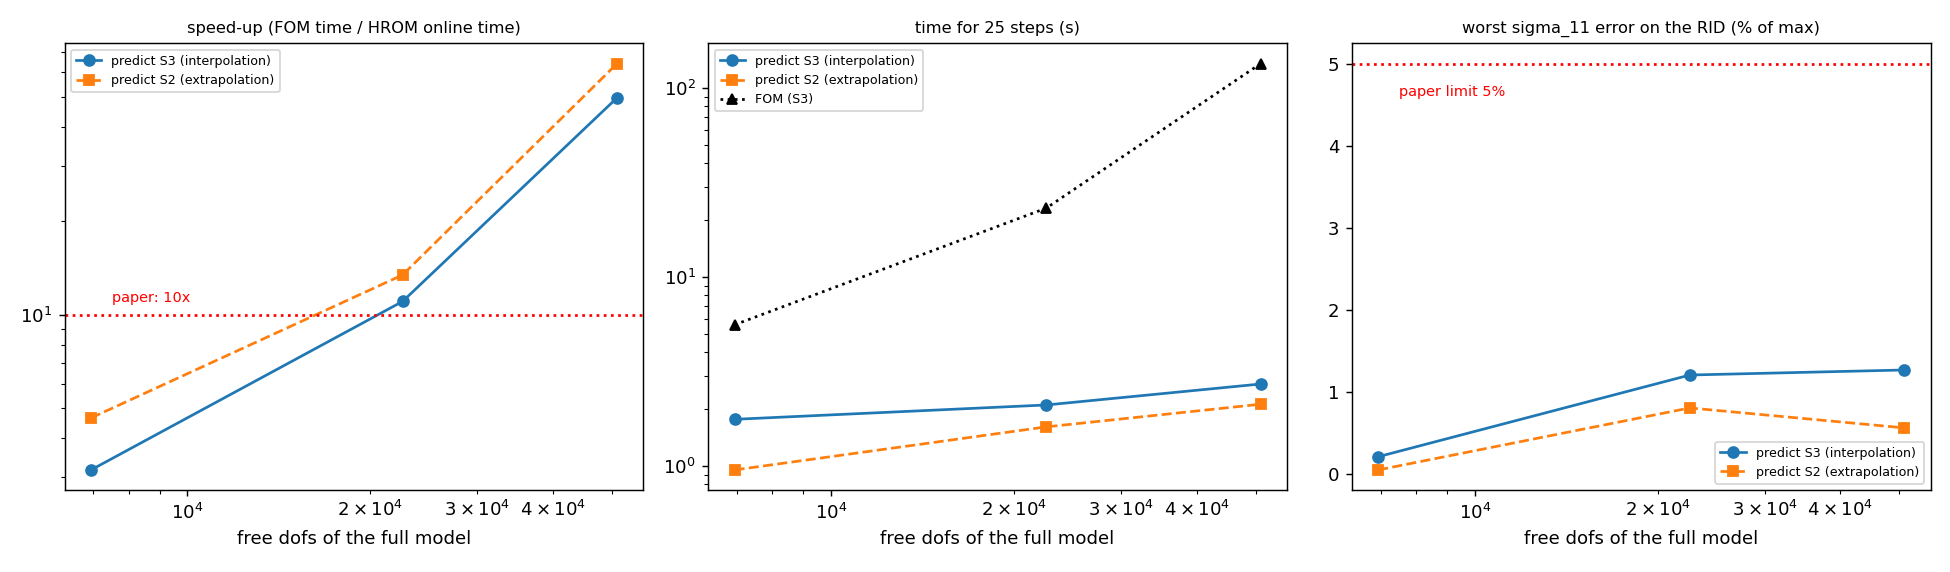
\includegraphics[width=0.95\linewidth]{figures/ch14r/hb3_mesh.png}
\caption{Mesh study: speed-up, computing time and worst $\sigma_{11}$ error against the number of free degrees of freedom, for S3 (solid) and the extrapolation case S2 (dashed); the red dotted lines are the publication's $10\times$ and $5\,\%$.}\label{fig:vf-hb3-mesh}
\end{figure}

A larger RID (two rings, or $d=0.3$~mm) covers more of the active pairs (130 of 221 with two layers on L2) but does not improve the errors usefully: displacement and stress errors change by less than $0.05$ percentage points, the force error stays at $7$--$9\,\%$ and the speed-up falls by half (L2: $49.7\times$ to $22.5\times$); the single-layer RID with $d=0.1$~mm remains the best trade-off. To test an edge case, S2 (the smallest radius, the largest gap) was predicted from S1, S3, S4, S5, so it lies outside the training range (\Cref{tab:vf-hb3-extra}); the case S6 ($R_p=3.98$~mm) never touches and is not a contact test.

\begin{table}[tbp]
\centering\footnotesize
\caption{Extrapolation to S2 ($R_p=4.02$ mm) from S1, S3, S4, S5.}\label{tab:vf-hb3-extra}
\begin{tabular}{@{}lrrrrrrr@{}}
\toprule
Mesh & RID elements & S2-active pairs in RID & Speed-up & Worst $u$ & Worst $\sigma_{11}$ & Worst force & Min.\ agreement\\
\midrule
L1 & 617 & 18/18 & 4.7$\times$ & 0.029\,\% & 0.050\,\% & 1.9\,\% & 100\,\%\\
L1.5 & 854 & 26/26 & 13.4$\times$ & 0.66\,\% & 0.81\,\% & 25.6\,\% & 92.7\,\%\\
L2 & 902 & 27/51 & 64.0$\times$ & 0.24\,\% & 0.56\,\% & 16.3\,\% & 100\,\%\\
\bottomrule
\end{tabular}
\end{table}

\subsection*{Comparison with the publication}

\begin{table}[tbp]
\centering\footnotesize
\caption{Outcome of the reproduction of \citet{fauque2018hybrid}.}\label{tab:vf-hb-cmp}
\begin{tabularx}{\linewidth}{@{}>{\raggedright\arraybackslash}p{4.3cm} >{\raggedright\arraybackslash}X >{\raggedright\arraybackslash}p{2.4cm}@{}}
\toprule
Result & This work & Outcome\\
\midrule
Rope, regular grid: displacement error (mean / max) & $0.74\,\%$ / $2.6\,\%$ against $0.34\,\%$ / $1.13\,\%$ & about 2$\times$ worse\\
Rope, regular grid: forces & $13\,\%$ / $67\,\%$ on RID with a $2.5\times$ larger RID; same HR-below-PB ordering & reproduced (ordering)\\
Rope, greedy: displacement error & $0.011\,\%$ / $0.084\,\%$ against $0.004\,\%$ / $0.077\,\%$ (RID of 70 nodes) & reproduced\\
Rope, greedy: force on RID & $0.45\,\%$ / $9.6\,\%$ against $0.34\,\%$ / $10\,\%$ & reproduced\\
Rope, greedy: reconstructed force & $10.3\,\%$ / $36\,\%$ against $1.3\,\%$ / $18\,\%$ & not reproduced\\
HR more accurate than PB in $H^1$ & yes with a large RID, weak with a small one & reproduced (large RID)\\
Rope speed-up & $0.6$--$1\times$ against $8.5\times$ & not reproduced\\
3D, publication's training set (S1+S2) & $13$--$19\,\%$ displacement error against $1\,\%$ & not reproduced\\
3D, with S4, S5 added & $0.05\,\%$ / $0.21\,\%$, correct contact set & reproduced, training set changed\\
3D speed-up & $3.7\times$ on the baseline mesh, $11\times$ and $50\times$ refined, against $10\times$ & partly\\
\bottomrule
\end{tabularx}
\end{table}

\subsection*{Open details and the speed-ups}

The publication leaves open several details that decide the numbers (\Cref{tab:vf-hb-gaps}); the final RID size and the contact-node set should be treated as free tuning parameters unless the authors' code is available. The speed-up on the rope is not reproduced because with a 70--90 node RID on a 100-node mesh there is little to gain, and the three-dimensional speed-up depends on a mesh size the publication does not state. The 4 against 1 dual mode count was not resolved, the reconstruction of forces outside the RID (\cref{eq:hb-nnls}) is worse than the publication's mean for reasons not investigated, and every test is interpolation inside the trained parameter range, with one mesh, one geometric parameter and no extrapolation except the one S2 case.

\begin{table}[tbp]
\centering\footnotesize
\caption{Information the publication does not give, what was assumed and the measured impact (selected).}\label{tab:vf-hb-gaps}
\begin{tabularx}{\linewidth}{@{}>{\raggedright\arraybackslash}p{4.2cm} >{\raggedright\arraybackslash}X >{\raggedright\arraybackslash}X@{}}
\toprule
Missing or ambiguous & Assumed & Measured impact\\
\midrule
Final RID size in the greedy and the rings around the DEIM elements & union of DEIM elements plus rings (best match: 3 rings, 70 of 98 nodes) & decisive: 1 ring $0.49\,\%$, 3 rings $0.011\,\%$, 8 rings $0.002\,\%$ (publication $0.004\,\%$)\\
Which nodes are potential contacts & nodes that ever carried a force, $\pm1$ node & with every RID node a contact the reduced matrix is exactly singular for small RIDs ($\sigma_{\min}/\sigma_{\max}\sim10^{-17}$)\\
Candidate set and first snapshot of the greedy & $20\times24$ uniform candidates, first at the centre & not decisive: greedy snapshots no better than 50 random ones\\
Number of dual modes & threshold as stated & 4 against 1; forcing 1 did not help alone\\
Sign of load and obstacle & mirrored: $f=+1$, $u\le d$ & none expected (exact mirror)\\
Active-set algorithm details & Lemke on the condensed problem (also a saddle-point active set) & both agree when the reduced matrix is non-singular\\
Mesh, element type and size, contact-pair matching (3D) & matching hexahedral meshes, node-to-node, radial gap & not tested\\
Young's modulus printed ``105 MPa'' & $10^5$ MPa & chosen to match the publication's gaps\\
Timing set-up behind the speed-ups & Python/NumPy, same machine & not comparable\\
\bottomrule
\end{tabularx}
\end{table}

\section{Projection-based reduction of contact}\label{sec:vf-bal}

\subsection*{Concept and purpose}

\citet{balajewicz2016contact} reduce Lagrange-multiplier contact by Galerkin projection with two bases of the same size: an SVD basis for the displacements, and a \emph{non-negative} basis for the contact forces, obtained by non-negative matrix factorisation (NMF), so that the reduced multipliers stay non-negative by construction. A greedy sampler chooses the training parameters with a contact-condition indicator that needs no linear solve. Three experiments test the method: a static membrane against a parametrised obstacle, its dynamic version, and two clamped plates in dynamic contact; the last also tests how far the temporal snapshots can be down-sampled. It is the method of Chapter~\ref{ch:hyper}, and the study checks what the packages already contain of it and what had to be added.

\subsection*{Mathematics as implemented}

The semi-discrete contact problem is $\mathbf M\ddot{\mathbf u}+\mathbf K\mathbf u=\mathbf f+\mathbf B^{T}\boldsymbol\lambda$, $\mathbf B\mathbf u-\mathbf c\ge\mathbf 0$, $\boldsymbol\lambda\ge\mathbf 0$, $\boldsymbol\lambda^{T}(\mathbf B\mathbf u-\mathbf c)=0$. After implicit time discretisation each step is the saddle-point problem
\begin{equation}\label{eq:bl-sp}
\min_{\mathbf v}\max_{\boldsymbol\mu\ge\mathbf 0}\ \tfrac12\mathbf v^{T}\mathbf A\mathbf v-\mathbf v^{T}\mathbf b-\boldsymbol\mu^{T}(\mathbf B\mathbf v-\mathbf c).
\end{equation}
With $\mathbf u\approx\mathbf U\mathbf u_r$ and $\boldsymbol\lambda\approx\mathbf U_\lambda\boldsymbol\lambda_r$, $\mathbf U_\lambda\ge\mathbf 0$, the reduced matrices are
\begin{equation}\label{eq:bl-red}
\mathbf A_r=\mathbf U^{T}\mathbf A\mathbf U,\qquad\mathbf B_r=\mathbf U_\lambda^{T}\mathbf B\mathbf U,\qquad\mathbf c_r=\mathbf U_\lambda^{T}\mathbf c,
\end{equation}
and the reduced multipliers $\boldsymbol\lambda_r\ge\mathbf 0$ give $\mathbf U_\lambda\boldsymbol\lambda_r\ge\mathbf 0$ automatically. The displacement basis $\mathbf U$ is a POD of the snapshots; the dual basis is the NMF of the multiplier snapshots,
\begin{equation}\label{eq:bl-nmf}
\mathbf X_\lambda\approx\mathbf U_\lambda\mathbf V_\lambda,\qquad\mathbf U_\lambda,\mathbf V_\lambda\ge\mathbf 0,
\end{equation}
computed by hierarchical alternating least squares with a non-negative SVD start (\anchor{rom_engine.nonneg_dual_basis}); contact-free (zero) dual snapshots are dropped.

\emph{Greedy sampling.} The next parameter is the candidate with the largest indicator
\begin{equation}\label{eq:bl-ind}
I=\sum_n\alpha_1\phi(\mathbf r_1)^2+\alpha_2\lVert\mathbf r_2\rVert^2+\alpha_3\phi(\mathbf r_3)^2,
\end{equation}
with the penetration $\mathbf r_1=\mathbf B\mathbf u-\mathbf c$, the complementarity $\mathbf r_2=\mathbf B^{+}(\mathbf A\mathbf u-\mathbf b)\odot(\mathbf B\mathbf u-\mathbf c)$, the force sign $\mathbf r_3=\mathbf B^{+}(\mathbf A\mathbf u-\mathbf b)$ and $\phi(\mathbf v)=\lVert[\mathbf v]_-\rVert$. No linear solve is needed. The error measures are squared relative norms in per cent (the publication's Eqs.~16--17), implemented literally.

\subsection*{What the packages provided}

\Cref{tab:vf-bl-cap} is the capability assessment made before the runs. The reduced-order side of the publication is implemented in \rom{} (\texttt{nonneg\_dual\_basis}, \texttt{ContactROM}, \texttt{solve\_reduced\_contact}, \texttt{contact\_condition\_indicator}, \texttt{greedy\_contact\_sampling}); the finite element side is adequate for plates and for complementarity-based contact up to a few thousand constraints, and four things were bridged with local code, each cross-checked against the package where they overlap.

\begin{table}[tbp]
\centering\footnotesize
\caption{Paper ingredient, package support and what was done.}\label{tab:vf-bl-cap}
\begin{tabularx}{\linewidth}{@{}>{\raggedright\arraybackslash}p{3.3cm} >{\raggedright\arraybackslash}p{3.2cm} >{\raggedright\arraybackslash}X@{}}
\toprule
Ingredient & Package support & Evidence or action\\
\midrule
Q4 scalar membrane (Laplace) element & missing in \fea{} & assembled locally (9-point stencil, lumped mass); free-membrane centre value $-0.7382$ against analytic $\approx-0.737$\\
Mindlin / Kirchhoff plate & Mindlin only & Mindlin used; clamped-plate centre deflection within $0.3\,\%$ of the analytic $0.00126\,qL^4/D$, first frequency within $0.4\,\%$ (24$\times$24 mesh)\\
Static contact solver & yes, dense (forms $\mathbf B\mathbf K^{-1}\mathbf B^{T}$) & fine to about 3k constraints, impossible at 39\,601 ($\approx12.5$ GB); a sparse primal--dual active-set solver was written and agrees with the package active-set, Lemke and projected-Gauss--Seidel solvers to $10^{-15}$ (check C1)\\
Dynamic contact solver & first-order two-step scheme only & free-vibration test: package scheme error $4.7\times10^{-2}$ at $\Delta t=2.5\times10^{-3}$ (order 1), local BDF2 $7.8\times10^{-4}$ (order 2) (C4); BDF2 contact stepping written locally\\
POD, SVD basis & yes & ---\\
NMF dual basis & yes & non-negative by construction (minimum entry $\ge10^{-17}$); fit within $1\,\%$ of SVD at rank 8 (C5)\\
Reduced contact solve & yes (static \texttt{ContactROM}, \texttt{solve\_reduced\_contact}) & full bases reproduce the full model to $2\times10^{-15}$ (C2); the reduced dynamic loop was written locally\\
Error indicator & yes & matches the vectorised formula exactly (C3: $0.77469$ both); the $\alpha_2,\alpha_3$ terms use a dense least-squares per call and do not scale, $\alpha=(1,0,0)$ is matrix-free\\
Greedy loop & yes & reproduced an independent implementation's selection sequence exactly (static, 20 iterations); trajectory snapshots, the $p(N_{\rm iter})$ growth schedule and the relative stopping test are not provided\\
\bottomrule
\end{tabularx}
\end{table}

The building-block checks are in \Cref{tab:vf-bl-checks}.

\begin{table}[tbp]
\centering\footnotesize
\caption{Building-block checks C1--C6.}\label{tab:vf-bl-checks}
\begin{tabularx}{\linewidth}{@{}>{\raggedright\arraybackslash}p{4.8cm} >{\raggedright\arraybackslash}X@{}}
\toprule
Check & Result\\
\midrule
C1 sparse PDAS against package active-set / Lemke / PGS (529-dof obstacle) & max difference $1.1\times10^{-15}$ / $7.8\times10^{-16}$ / $7.8\times10^{-16}$\\
C2 \texttt{ContactROM} with $\mathbf U=\mathbf U_\lambda=\mathbf I$ against full & $1.7\times10^{-15}$ ($u$), $2.1\times10^{-15}$ ($\lambda$)\\
C3 package indicator against local, $\alpha=(1,1,1)$ & $0.7746922$ against $0.7746922$\\
C4 free-membrane error at $t=2$ ($\Delta t=10^{-2}$, $5\times10^{-3}$, $2.5\times10^{-3}$) & BDF2 $1.2\times10^{-2}$, $3.1\times10^{-3}$, $7.8\times10^{-4}$ (order 2); package two-step $1.6\times10^{-1}$, $8.7\times10^{-2}$, $4.7\times10^{-2}$ (order 1)\\
C5 NMF against SVD relative fit, rank 4 / 8 / 16 & $0.385$ / $0.0249$ / $1.4\times10^{-9}$ against $0.377$ / $0.0247$ / $5.7\times10^{-16}$; the SVD basis has minimum entry $-0.97$ to $-1.0$, NMF $\ge0$\\
C6 reduced complementarity solve, $p=20/40/100/200$ & 1.0 / 1.4 / 1.9 / 8.0 ms\\
\bottomrule
\end{tabularx}
\end{table}

\subsection*{Geometry and mesh}

\emph{Static and dynamic membrane.} A membrane on the unit square, $200\times200$ bilinear elements (39\,601 degrees of freedom) in the static case and $40\times40$ (1521) in the dynamic case, loaded by a uniform load $-10$ ($-\nabla^2u=f$, so the membrane deflects downward as in the publication's figure) and held up by an obstacle of two Gaussian bumps whose position $\gamma_1$ and height $\gamma_2$ are the parameters, $\gamma\in[0.3,0.6]\times[0.2,0.6]$ (\Cref{fig:vf-bl-obstacle}). \emph{Two plates.} Two identical clamped steel plates ($L=1$~m, $h=1$~mm, $\rho=7800$, $E=200$~GPa, $\nu=0.3$) with a $4$~cm gap, each meshed with $24\times24$ Mindlin elements, 3174 degrees of freedom and 529 gap constraints at facing nodes (the publication's plates are Kirchhoff plates with one degree of freedom per node and 20\,000 in all); a pressure pulse acts only on the lower plate (\Cref{fig:vf-bl-two}). \Cref{tab:vf-bl-setup} lists the settings.

\begin{figure}[tbp]
\centering
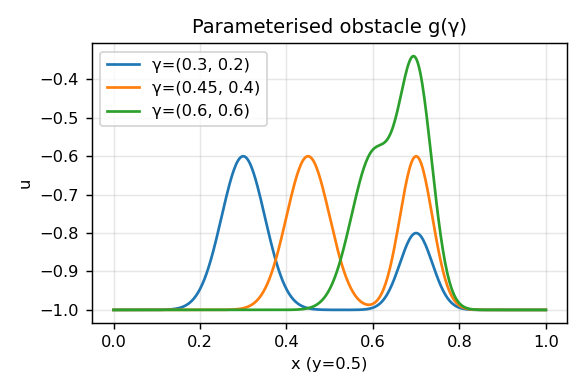
\includegraphics[width=0.7\linewidth]{figures/ch14r/bl_obstacle.png}
\caption{Obstacle of the membrane problem and its parametrisation.}\label{fig:vf-bl-obstacle}
\end{figure}

\begin{figure}[tbp]
\centering
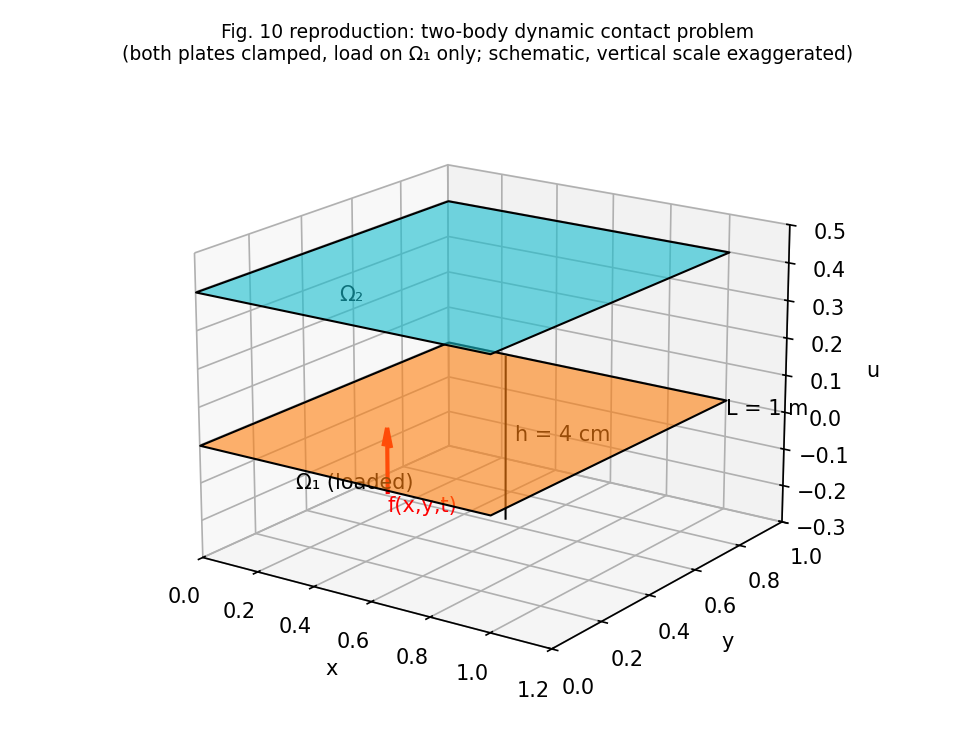
\includegraphics[width=0.6\linewidth]{figures/ch14r/bl_two.png}
\caption{Two-body set-up: two clamped plates with a 4~cm gap and a pressure pulse on the lower plate; the non-penetration constraint is imposed at every pair of facing nodes (529). Redrawn schematic, vertical scale exaggerated; not simulation output.}\label{fig:vf-bl-two}
\end{figure}

\begin{table}[tbp]
\centering\footnotesize
\caption{Set-up of the three experiments.}\label{tab:vf-bl-setup}
\begin{tabularx}{\linewidth}{@{}>{\raggedright\arraybackslash}p{2.6cm} >{\raggedright\arraybackslash}X >{\raggedright\arraybackslash}X >{\raggedright\arraybackslash}X@{}}
\toprule
 & Static obstacle & Dynamic obstacle & Two plates\\
\midrule
Size, this work (publication) & 39\,601 (40\,000) dofs & 1521 (40\,000) dofs & 3174 (20\,000) dofs\\
Time stepping & --- & BDF2 (BDF1 first step), $\Delta t=0.005$, 400 steps & BDF2, $\Delta t=2\times10^{-4}$, 2000 steps\\
Parameters & $\gamma\in[0.3,0.6]\times[0.2,0.6]$, $10\times10$ candidates & same range & non-parametric (reproduction mode, one parameter)\\
Greedy & 20 iterations, $p=p_\lambda=N_{\rm iter}$, first sample candidate 0 & 10 iterations, $p=p_\lambda=\lfloor2+(N_{\rm iter}-1)\,98/9\rfloor$ (2 to 100) & $p=p_\lambda=40$, all 2001 steps\\
Bases & snapshots used directly & SVD primal, NMF dual (150 HALS iterations) on active columns & as dynamic\\
Reference for errors & Eq.~16 on the 100 candidates; random sampling: 50 Latin hypercube draws of 20 samples & Eq.~17 over all time steps & Eq.~17 on $w$\\
\bottomrule
\end{tabularx}
\end{table}

\subsection*{Results: static obstacle (paper Figs.~3--5, full size)}

\Cref{tab:vf-bl-static} and \Cref{fig:vf-bl-static} give the greedy convergence. After 20 greedy samples the maximum error with $\alpha=(1,0,0)$ is $5.0\times10^{-4}\,\%$, a factor of 124 below the median of random sampling (median $6.3\times10^{-2}\,\%$, minimum $2.0\times10^{-2}$, maximum $0.22$), and the greedy loop with 10 samples ($4.4\times10^{-2}\,\%$) already beats the median of 20 random samples, as the publication states. The three indicator weightings $\alpha=(1,1,1)$, $(1,1,0)$, $(1,0,0)$ gave the \emph{identical} selection sequence ($0$, $99$, $64$, $92$, $44$, $80$, \dots) and errors, so the publication's difference between them was not reproduced; the oracle greedy on the true error is worse than the indicator-driven one from $N_{\rm iter}\ge13$ ($1.7\times10^{-3}\,\%$ against $5.0\times10^{-4}\,\%$ at 20), because greedy on the maximum error is myopic; and the package's \texttt{greedy\_contact\_sampling} gave the identical 20-element sequence as the local loop.

\begin{table}[tbp]
\centering\footnotesize
\caption{Static obstacle, $N_{\rm iter}=20$.}\label{tab:vf-bl-static}
\begin{tabular}{@{}lrr@{}}
\toprule
Quantity & Publication & This work\\
\midrule
Max relative error, greedy $\alpha=(1,0,0)$ & ``an order of magnitude'' below random $p=20$ & $5.0\times10^{-4}\,\%$ against random median $6.3\times10^{-2}\,\%$ ($124\times$ lower)\\
Greedy at $p\approx10$ against random $p=20$ & equal accuracy & $4.4\times10^{-2}\,\%<6.3\times10^{-2}\,\%$\\
Mean relative error, greedy 20 & --- & $3.6\times10^{-5}\,\%$ (random median $6.5\times10^{-3}\,\%$)\\
Indicator weights & $\alpha_1$ only is best & identical sequences\\
Oracle on the true error & lowest curve & worse at $N_{\rm iter}\ge13$\\
\bottomrule
\end{tabular}
\end{table}

\begin{figure}[tbp]
\centering
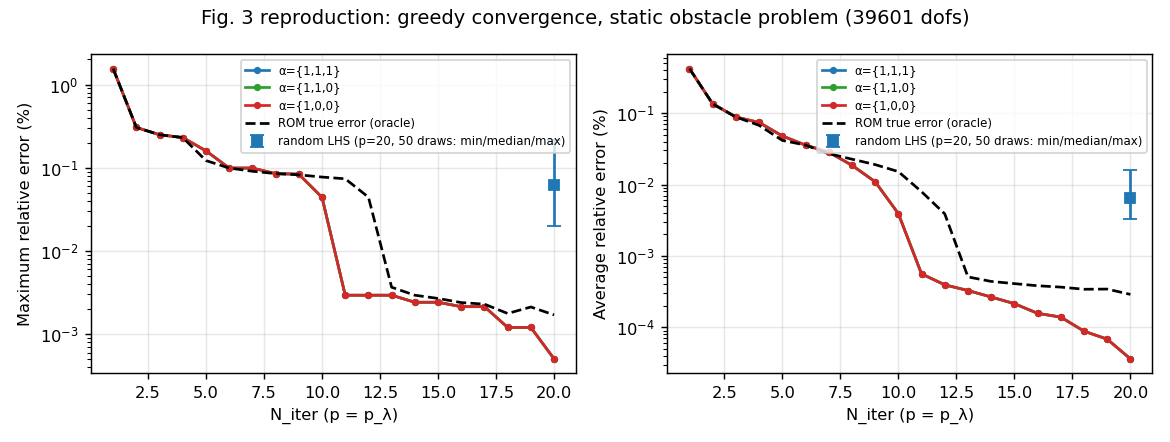
\includegraphics[width=0.9\linewidth]{figures/ch14r/bl_static.png}
\caption{Static obstacle, greedy convergence against random sampling for the indicator weightings and the oracle.}\label{fig:vf-bl-static}
\end{figure}

\begin{figure}[tbp]
\centering
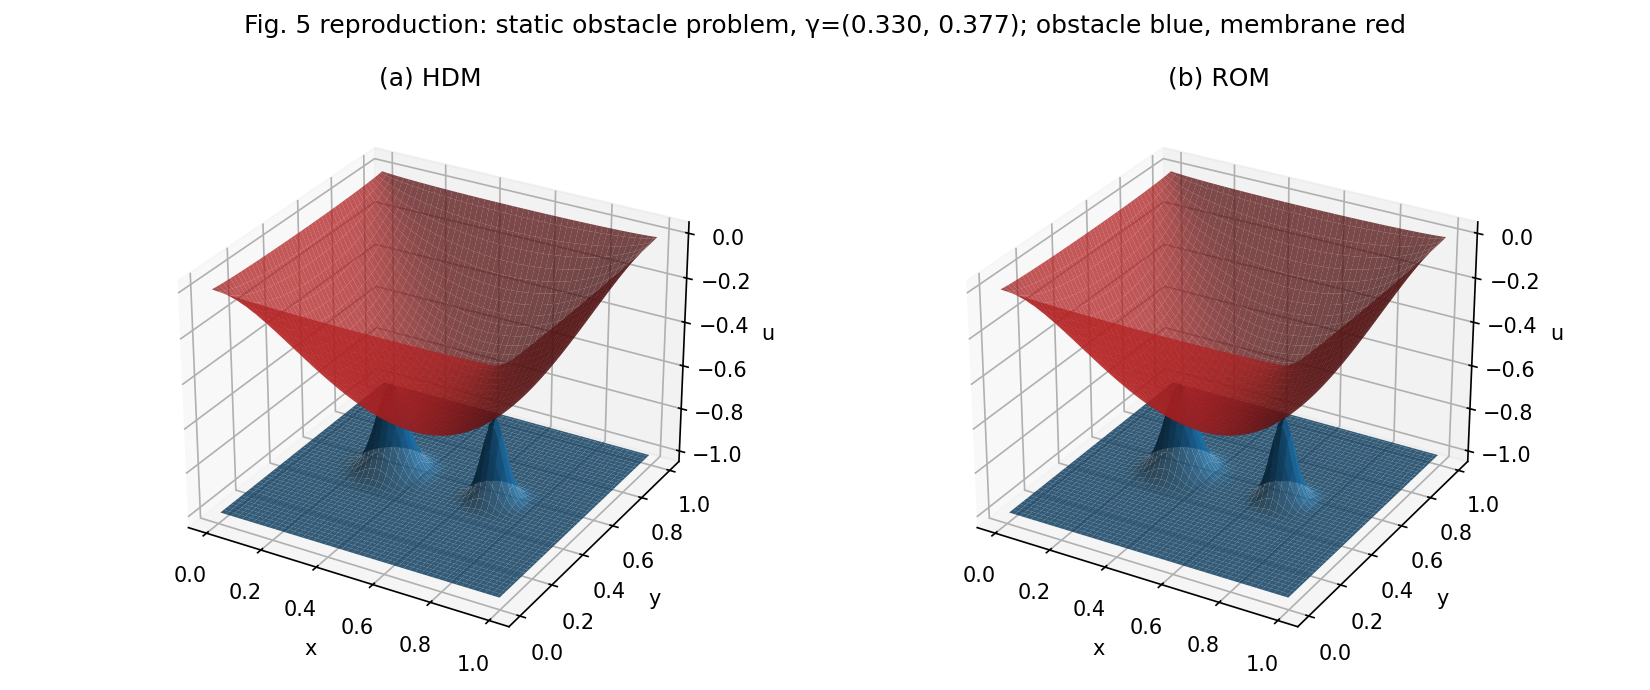
\includegraphics[width=0.9\linewidth]{figures/ch14r/bl_static3d.png}
\caption{Static solution: the membrane (red) sags under the load and is held by the two bump tips of the obstacle (blue), left bump at $x=\gamma_1=0.33$ and right bump at $x=0.7$ with height $\gamma_2$. The ROM built from 20 greedy snapshots ($p=p_\lambda=20$, 39\,601-dof full model) is visually indistinguishable from the full model.}\label{fig:vf-bl-static3d}
\end{figure}

At the publication's worst parameter $\gamma=(0.330,0.377)$ (off the grid) the displacement error is $1.5\times10^{-5}\,\%$, but the contact-force error is $52\,\%$ with an active-set overlap of $0.69$: displacement accuracy hides a poorer multiplier, which the publication does not report. Positivity over the 100 candidates ($p=p_\lambda=20$): the NMF dual basis gives minimum multiplier $0$ and worst full-space penetration $-1.3\times10^{-2}$ (only the projected constraint $\mathbf U_\lambda^{T}(\mathbf B\mathbf u-\mathbf c)\ge0$ is enforced); an SVD dual basis (not in the publication for the static case) gives minimum multiplier $-0.108$, penetration $-0.148$ and a maximum error of $4.0\,\%$ (mean $2.3\,\%$), about four orders worse.

\subsection*{Results: dynamic obstacle (paper Figs.~6--9)}

On the $40\times40$ mesh the error falls by a factor of 127 to 288 over ten greedy iterations for all indicator weightings (\Cref{tab:vf-bl-dyn}, \Cref{fig:vf-bl-dyn}), the publication's ``more than $100\times$ after 10 iterations, all strategies equal''; a candidate sweep of the final $\alpha=(1,0,0)$ ROM gives maximum $0.145\,\%$ and mean $0.070\,\%$.

\begin{table}[tbp]
\centering\footnotesize
\caption{Dynamic obstacle: maximum relative error (Eq.~17, \%) by iteration.}\label{tab:vf-bl-dyn}
\begin{tabular}{@{}lrrrrr@{}}
\toprule
Weights & $N_{\rm iter}=1$ & 2 & 5 & 10 & Reduction 1$\to$10\\
\midrule
$\alpha=(1,1,1)$ & 41.8 & 4.41 & 0.805 & 0.153 & 273$\times$\\
$\alpha=(1,1,0)$ & 41.8 & 10.9 & 0.808 & 0.329 & 127$\times$\\
$\alpha=(1,0,0)$ & 41.8 & 10.9 & 0.711 & 0.145 & 288$\times$\\
Oracle (true error) & 41.8 & 6.03 & 0.745 & 0.300 & 139$\times$\\
\bottomrule
\end{tabular}
\end{table}

\begin{figure}[tbp]
\centering
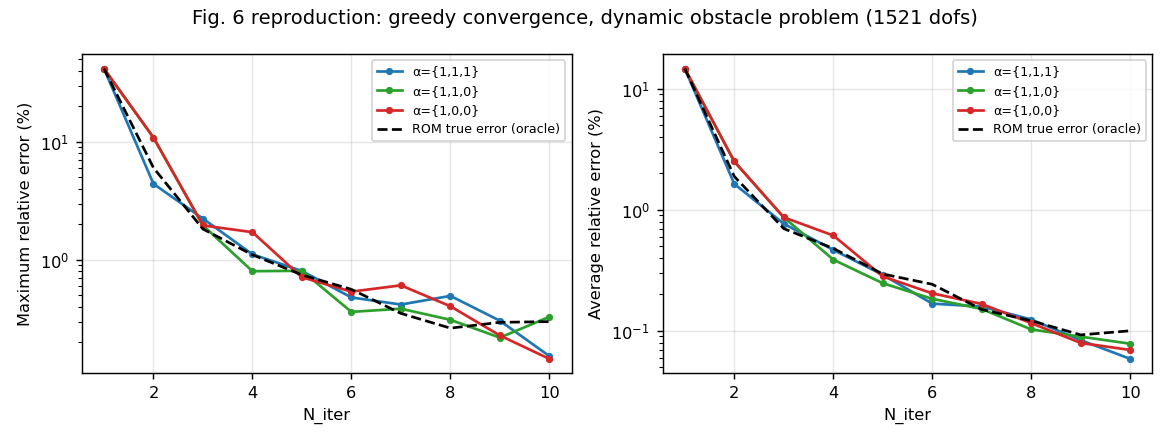
\includegraphics[width=0.9\linewidth]{figures/ch14r/bl_dyn.png}
\caption{Dynamic obstacle, greedy convergence.}\label{fig:vf-bl-dyn}
\end{figure}

\begin{figure}[tbp]
\centering
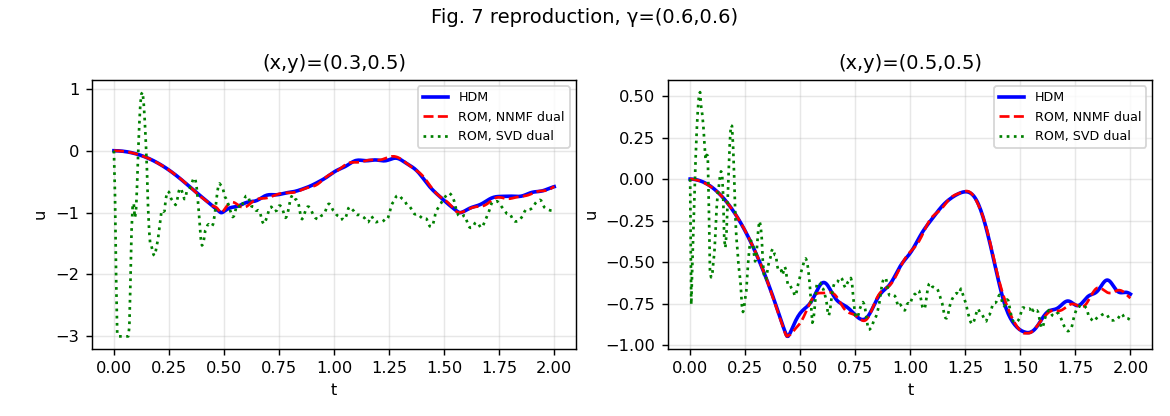
\includegraphics[width=0.95\linewidth]{figures/ch14r/bl_hist.png}
\caption{Time history of the final ROM ($p=p_\lambda=100$) at the off-training test parameter $\gamma=(0.6,0.6)$.}\label{fig:vf-bl-hist}
\end{figure}

\Cref{tab:vf-bl-nmf} gives the publication's central qualitative claim at two test parameters: the SVD-dual ROM fails because positivity is lost (errors of about $300\,\%$, negative multipliers down to $-714$, penetrations more than 15 times the membrane depth), while the NMF-dual ROM tracks the full model. The field at $t=0.2$ for the worst-case test parameter is reproduced in shape and contact region (error $0.058\,\%$, \Cref{fig:vf-bl-dyn3d}).

\begin{table}[tbp]
\centering\footnotesize
\caption{NMF against SVD dual basis, dynamic obstacle.}\label{tab:vf-bl-nmf}
\begin{tabular}{@{}lrrr@{}}
\toprule
Test $\gamma$ & NMF dual: error / min $\lambda$ / min gap & SVD dual: error / min $\lambda$ / min gap\\
\midrule
$(0.6,0.6)$ & $0.083\,\%$ / 0 / $-1.5\times10^{-2}$ & $307\,\%$ / $-664$ / $-15.5$\\
$(0.300,0.288)$ & $0.058\,\%$ / 0 / $-1.3\times10^{-2}$ & $296\,\%$ / $-714$ / $-17.6$\\
\bottomrule
\end{tabular}
\end{table}

\begin{figure}[tbp]
\centering
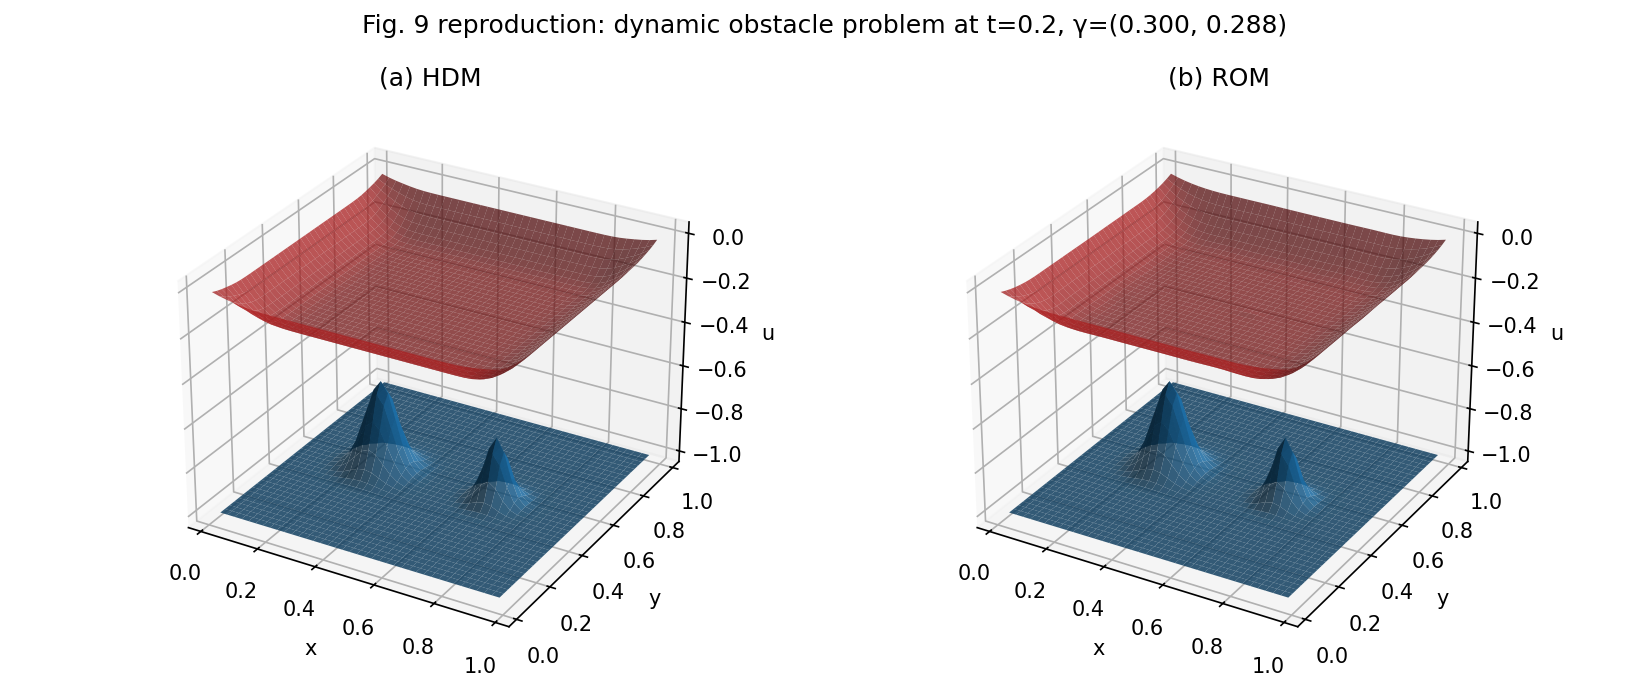
\includegraphics[width=0.9\linewidth]{figures/ch14r/bl_dyn3d.png}
\caption{Dynamic obstacle at $t=0.2$, $\gamma=(0.300,0.288)$: the 1521-dof full model against the NMF-dual ROM ($p=p_\lambda=100$); the membrane is still moving.}\label{fig:vf-bl-dyn3d}
\end{figure}

\begin{figure}[tbp]
\centering
\includegraphics[width=1.0\linewidth]{figures/ch14_bal.pdf}
\caption{Dynamic obstacle problem of \citet{balajewicz2016contact} (1\,521 dofs). (a) Maximum error against the greedy iteration for the three indicator weightings and the true-error oracle (a reduction of \cvfBalRed{} for $\alpha=(1,0,0)$). (b), (c) Response at a test parameter: the NMF dual basis follows the full-order model (error \cvfBalNmf), the SVD dual basis does not (error \cvfBalSvd). Measured speed-up \cvfBalSpeed.}\label{fig:vf-bal}
\end{figure}

\subsection*{Results: two-body dynamic contact (paper Figs.~10--13)}

Contact is active in 366 of the 2000 steps; the plate-centre amplitude is $0.126$~m (the publication's axis spans $\pm0.2$~m) and the peak contact force is $1.7\times10^3$~N per node (\Cref{fig:vf-bl-twohist}). \Cref{tab:vf-bl-two} gives the ROMs against a full-order run of $10.0$~s: the NMF dual with $p=p_\lambda=40$ (the publication's choice) has an error of $1.36\,\%$ and runs $13.5$ times faster, while the SVD dual of the same size fails ($41\,\%$, minimum multiplier $-2.9\times10^6$). At the single instant $t=0.4$~s the full-state field error of the $p=40$ ROM is $25\,\%$ (all degrees of freedom including rotations), far larger than the $1.4\,\%$ time-integrated error on $w$; the 3D snapshot looks close but is the harder test (\Cref{fig:vf-bl-two3d}).

\begin{table}[tbp]
\centering\footnotesize
\caption{Two plates: error (Eq.~17 on $w$), minimum multiplier, minimum gap and online time against the full model (10.0~s).}\label{tab:vf-bl-two}
\begin{tabular}{@{}lrrrr@{}}
\toprule
ROM & Error & Min $\lambda$ & Min gap (m) & Online time\\
\midrule
NMF dual, $p=p_\lambda=20$ & $1.84\,\%$ & 0 & $-6.7\times10^{-3}$ & 0.41 s (24.7$\times$)\\
\textbf{NMF dual, $p=p_\lambda=40$} & $\mathbf{1.36\,\%}$ & 0 & $-1.2\times10^{-2}$ & 0.74 s (13.5$\times$)\\
NMF dual, $p=p_\lambda=100$ & $0.040\,\%$ & 0 & $-1.7\times10^{-3}$ & 1.59 s (6.3$\times$)\\
SVD dual, $p=p_\lambda=40$ & $41\,\%$ & $-2.9\times10^{6}$ & $-0.50$ & 4.8 s (2.1$\times$)\\
\bottomrule
\end{tabular}
\end{table}

\begin{figure}[tbp]
\centering
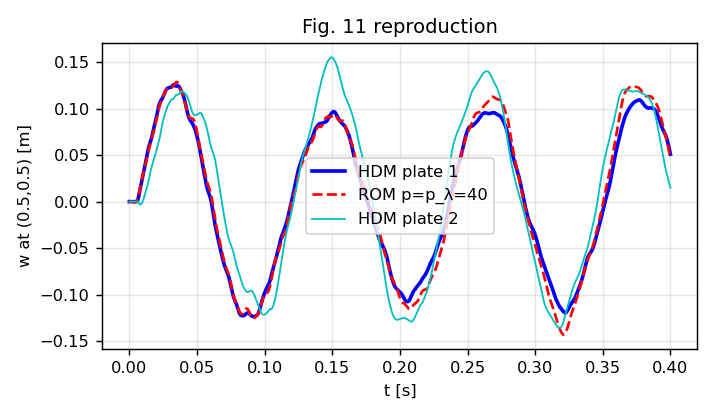
\includegraphics[width=0.95\linewidth]{figures/ch14r/bl_twohist.png}
\caption{Two plates: plate-centre time histories of the full model and the reduced models.}\label{fig:vf-bl-twohist}
\end{figure}

\begin{figure}[tbp]
\centering
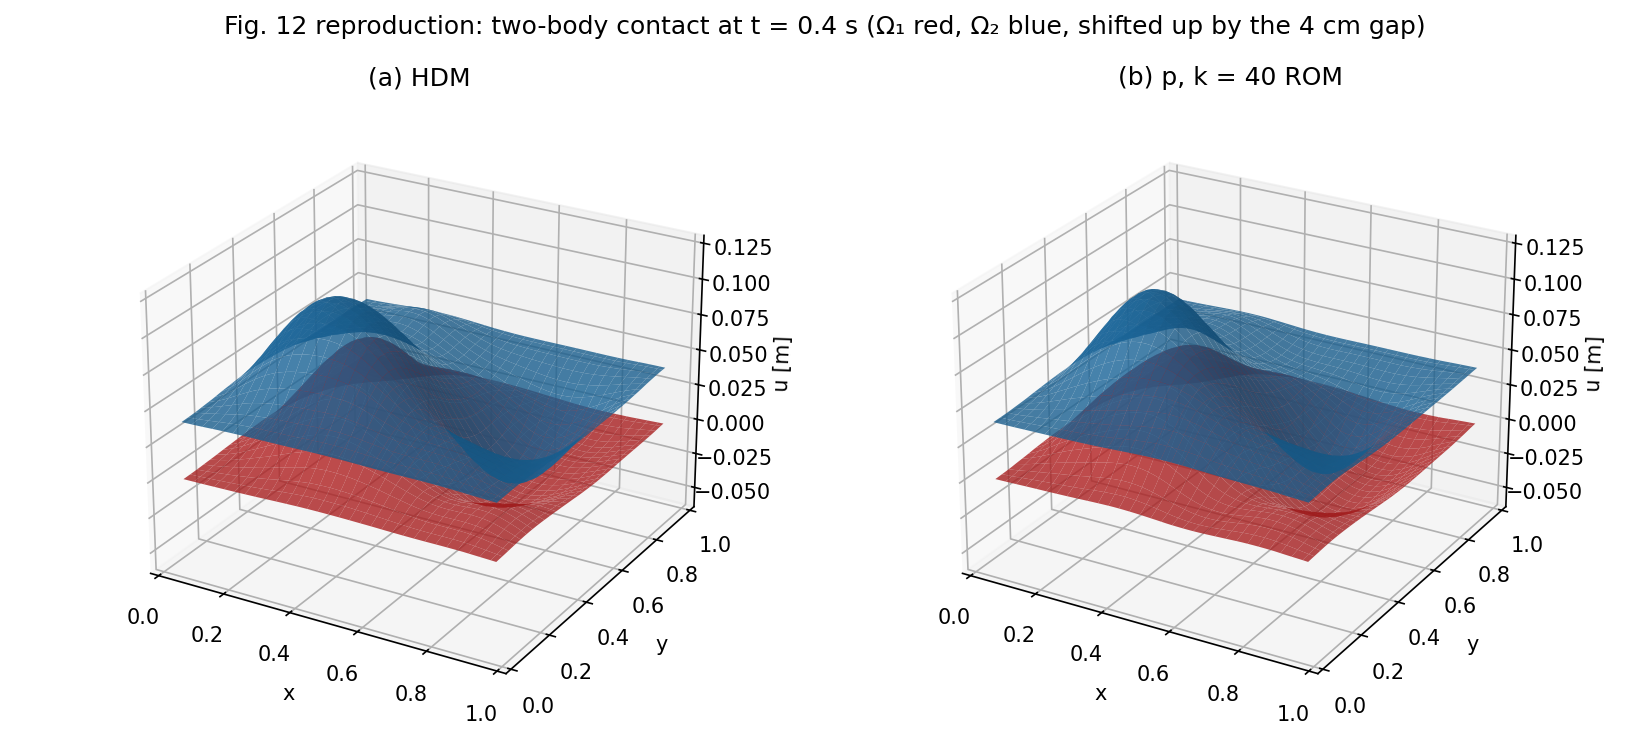
\includegraphics[width=0.95\linewidth]{figures/ch14r/bl_two3d.png}
\caption{Both plates at $t=0.4$~s: full model (left) and the $p=p_\lambda=40$ ROM (right); $\Omega_1$ red, $\Omega_2$ blue (shifted up by the gap so that touching surfaces coincide).}\label{fig:vf-bl-two3d}
\end{figure}

\emph{Down-sampling.} \Cref{tab:vf-bl-down} and \Cref{fig:vf-bl-down} give the error against the percentage of snapshots kept (25 snapshots is $1.25\,\%$). The error is flat down to about $10\,\%$ kept ($p=40$: $0.7$--$1.6\,\%$) and rises sharply at $5\,\%$ or less, as in the publication; its $52.8\,\%$ at 25 snapshots is not matched (here $13.6\,\%$). The $p=20$ curve is erratic and non-monotone, which points to local minima of the NMF and rank limits and not to the number of snapshots.

\begin{table}[tbp]
\centering\footnotesize
\caption{Two plates: error (\%) against the percentage of snapshots kept.}\label{tab:vf-bl-down}
\begin{tabular}{@{}lrrrrrrr@{}}
\toprule
\% kept & 100 & 50 & 25 & 10 & 5 & 2.5 & 1.25\\
\midrule
$p=p_\lambda=20$ & 1.84 & 10.3 & 2.83 & 4.23 & 6.54 & 3.64 & 15.0\\
$p=p_\lambda=40$ & 1.36 & 1.63 & 0.70 & 0.67 & 4.28 & 2.51 & 13.6\\
$p=p_\lambda=100$ & 0.040 & 0.042 & 0.099 & 0.50 & 1.21 & 2.59 & 13.6\\
\bottomrule
\end{tabular}
\end{table}

\begin{figure}[tbp]
\centering
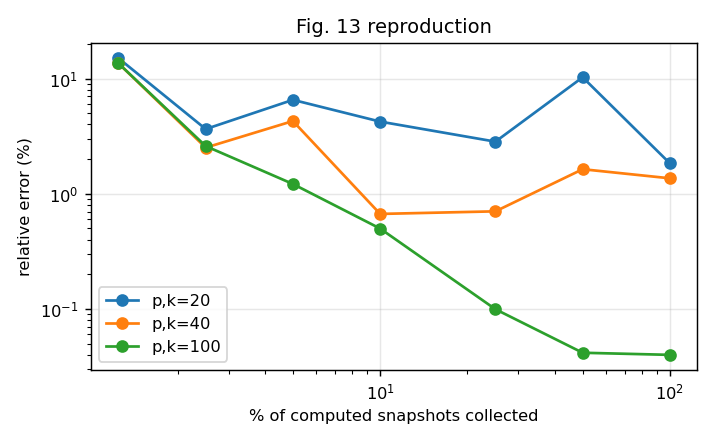
\includegraphics[width=0.7\linewidth]{figures/ch14r/bl_down.png}
\caption{Two plates: error against the percentage of snapshots kept.}\label{fig:vf-bl-down}
\end{figure}

\subsection*{Speed-ups}

\Cref{tab:vf-bl-speed} compares with the publication. The comparison is not one-to-one: the publication's full-order solver used MATLAB \texttt{quadprog} (interior point), here a sparse active-set solver with warm starts (membranes) or a precomputed dense complementarity matrix (plates) is used, much faster per solve; and the ROM cost is not strictly size-independent (a dense Cholesky of the reduced matrix at every step). The robust conclusion is the trend: ROM cost is independent of $N$ while full-order cost grows at least linearly, so the speed-up grows with mesh size.

\begin{table}[tbp]
\centering\footnotesize
\caption{Speed-up against the publication's Table~I.}\label{tab:vf-bl-speed}
\begin{tabularx}{\linewidth}{@{}>{\raggedright\arraybackslash}p{2.6cm} >{\raggedright\arraybackslash}X >{\raggedright\arraybackslash}X@{}}
\toprule
Problem & Publication (full-order size, ROM size, speed-up) & This work\\
\midrule
Static obstacle & 40\,000; $p=p_\lambda=20$; 865 & 39\,601; 20/20; 1256 (full 3.72 s sparse PDAS, ROM 3.0 ms)\\
Dynamic obstacle & 40\,000; 100; 302 & 1521; 100; 14.7 measured (3.59 s, 0.245 s); about 490 extrapolated to 39\,601 dofs (119 s per run), not measured\\
Two-body & 20\,000; 40; 2229 & 3174; 40; 13.5\\
\bottomrule
\end{tabularx}
\end{table}

\subsection*{Comparison with the publication}

\begin{table}[tbp]
\centering\footnotesize
\caption{Outcome of the reproduction of \citet{balajewicz2016contact}.}\label{tab:vf-bl-cmp}
\begin{tabularx}{\linewidth}{@{}>{\raggedright\arraybackslash}p{4.3cm} >{\raggedright\arraybackslash}X >{\raggedright\arraybackslash}p{2.5cm}@{}}
\toprule
Claim & This work & Outcome\\
\midrule
Greedy beats random sampling; $p\approx10$ equals random $p=20$ (static) & $124\times$ below the random median; yes & reproduced\\
$\alpha_1$-only indicator best & identical sequences (static); $\alpha_1$-only and all-three best by a small margin (dynamic) & not reproduced\\
More than $100\times$ error drop in 10 iterations (dynamic) & $127$--$288\times$ & reproduced\\
NMF dual tracks the full model, SVD dual does not & $0.06$--$0.08\,\%$ against $\sim300\,\%$ & reproduced\\
Two plates: $p=p_\lambda=40$ tracks the full model & $1.36\,\%$ (Mindlin, 3174 dofs) & reproduced, smaller mesh\\
Insensitive to down-sampling down to about $10\,\%$ & flat to $10\,\%$, rises at $\le5\,\%$; $52.8\,\%$ at 25 snapshots not matched ($13.6\,\%$) & partly\\
Speed-ups 865, 302, 2229 & 1256, 14.7, 13.5 (different solver, smaller meshes) & not comparable\\
\bottomrule
\end{tabularx}
\end{table}

\subsection*{Differences in scale and model form}

The static case is at the publication's size, but the dynamic and two-body cases are smaller (running the dynamic cases at the publication's size needs roughly 100 times the compute used). The plates are Mindlin elements with three degrees of freedom per node, where the publication has a Kirchhoff plate with one: linear deflection and frequency agree with Kirchhoff theory to better than $0.5\,\%$, but the contact response will differ in detail, and the publication gives no numbers beyond the $\pm0.2$~m range of its Fig.~11 to compare. The membrane discretisation is not specified beyond ``$200\times200$ elements''. The first greedy sample, the NMF algorithm and iteration count, the stopping parameter and the sign convention are unspecified and were chosen here. The oracle curve of the publication is the lowest, and the author's oracle (greedy on the true maximum error) is not, since its definition is open. Multiplier accuracy is weaker than displacement accuracy (static worst case $52\,\%$ force error, active-set overlap $0.69$) and the full-space penetration of the NMF ROM is non-zero, a point the publication does not report. Each configuration is a single run, wall-clock numbers are indicative only, and the full-size dynamic and 20\,000-degree-of-freedom plate cases were not run.

Four things were added or are recommended for the packages as a result: a scalar Laplace element and a sparse, non-condensed unilateral solver in \fea{} (the condensed route is fine to roughly 3000 constraints, an estimate and not a measured limit, and needs about 12.5~GB at 39\,601); BDF2 or Newmark in \texttt{solve\_contact\_dynamics} (the first-order scheme has about 28 times the BDF2 error at $\Delta t=0.005$ and about 60 times at $0.0025$, one free-membrane test); a \texttt{ContactROM.solve\_dynamic} with trajectory snapshots and the greedy growth schedule in \rom{}; and a cached pseudo-inverse in the indicator so that $\alpha_2,\alpha_3$ are usable at scale.

\section{Assembly reduction with contact and geometric nonlinearity}\label{sec:vf-asm}

\subsection*{Concept and purpose}

\citet{nikiema2026assembly} compare four reduced models for bolted-type assemblies that are preloaded and then loaded further: projection by POD alone, and POD with hyper-reduction by the energy-conserving sampling and weighting method (ECSW), the discrete empirical interpolation method (DEIM) and its unsymmetric variant (UDEIM). The assembly is geometrically nonlinear (total-Lagrangian Saint Venant--Kirchhoff material) and has unilateral contact between its parts. The study rebuilds the 2D benchmark from the text, then generalises the pipeline to 3D (Hex8 and Hex20 elements, an assembly builder, a full-order driver for sequential preloads). The central claims to test are that DEIM and UDEIM fail with plain Newton when the contact force is approximated, that POD and ECSW do not, and that domain partitioning (DP) gives a further saving.

\subsection*{Mathematics as implemented}

The element is total Lagrangian with the Saint Venant--Kirchhoff law: Green--Lagrange strain $\mathbf E=\tfrac12(\mathbf F^{T}\mathbf F-\mathbf I)$, second Piola--Kirchhoff stress $\mathbf S=\lambda\,\mathrm{tr}(\mathbf E)\mathbf I+2\mu\mathbf E$ (plane stress for the 2D element, \anchor{fea_engine.Quad4PlaneStressTL}), internal force $\mathbf f_{\rm int}(\mathbf u)=\int\mathbf B(\mathbf u)^{T}\mathbf S\,\mathrm dV$ and consistent tangent. The reduced model is
\begin{equation}\label{eq:as-pod}
\mathbf u\approx\mathbf V\mathbf q,\qquad\mathbf V^{T}\bigl[\mathbf f_{\rm int}(\mathbf V\mathbf q)+\mathbf f_{\rm c}(\mathbf V\mathbf q)-\mathbf f_{\rm ext}\bigr]=\mathbf 0,
\end{equation}
with $\mathbf V$ the POD of the snapshots at the chosen tolerance $\varepsilon$ on the discarded energy. The hyper-reduced variants replace the projected force by an approximation.

\emph{ECSW} evaluates the projected force on a weighted subset $\mathcal E$ of elements,
\begin{equation}\label{eq:as-ecsw}
\mathbf V^{T}\mathbf f(\mathbf V\mathbf q)\approx\sum_{e\in\mathcal E}\xi_e\,\mathbf V^{T}\mathbf L_e^{T}\mathbf f_e(\mathbf L_e\mathbf V\mathbf q),\qquad\xi_e\ge0,
\end{equation}
with weights from a non-negative least-squares fit to the snapshot force contributions up to a tolerance $\tau$.

\emph{DEIM and UDEIM} approximate the nonlinear force vector by interpolation on a basis $\mathbf\Phi_f$ of force snapshots at selected rows $\mathbf P$,
\begin{equation}\label{eq:as-deim}
\mathbf f\approx\mathbf\Phi_f(\mathbf P^{T}\mathbf\Phi_f)^{-1}\mathbf P^{T}\mathbf f,
\end{equation}
applied to the internal force (DEIM) or to the unassembled element forces (UDEIM); the tangent is approximated in the same way. In the variant added in this study (DEIM-NL, UDEIM-NL) the nonlinear forces include the contact force within the approximated term.

\emph{Domain partitioning.} The package's indicator splits the elements into a part that stays linear and a part that is nonlinear; only the latter is re-assembled in the Newton loop, and only the former is condensed once.

\subsection*{Geometry and mesh: 2D benchmark}

The 2D benchmark is a top-hat strip placed on a flat strip, 100~mm long with a 2.5~mm section, meshed by 324 four-node elements (800 free degrees of freedom); contact acts between the lower face of the top-hat and the flat strip. The parameters \emph{as stated} in the publication leave the upper part far too soft: contact begins in the first load increment, at 0.46~N, whereas the publication has it in the second. \Cref{fig:vf-as-geom} and \Cref{fig:vf-as-mesh} show the geometry and the mesh; \Cref{fig:vf-as-defo} the full-order deformed state.

\begin{figure}[tbp]
\centering
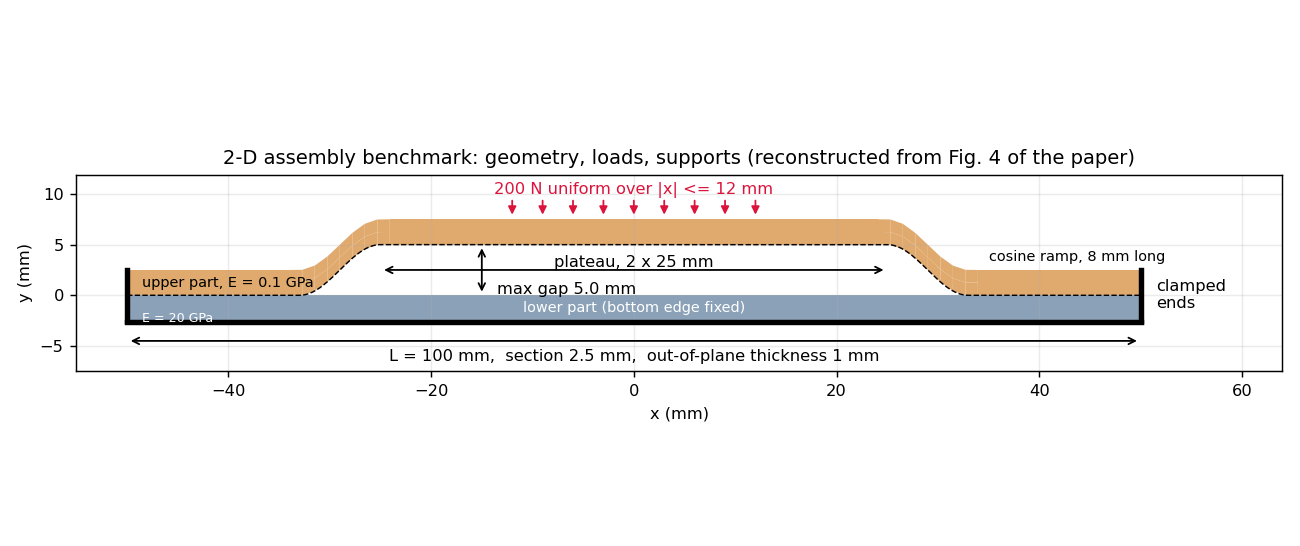
\includegraphics[width=0.95\linewidth]{figures/ch14r/as_geometry.png}
\caption{2D benchmark: the top-hat strip on the flat strip.}\label{fig:vf-as-geom}
\end{figure}

\begin{figure}[tbp]
\centering
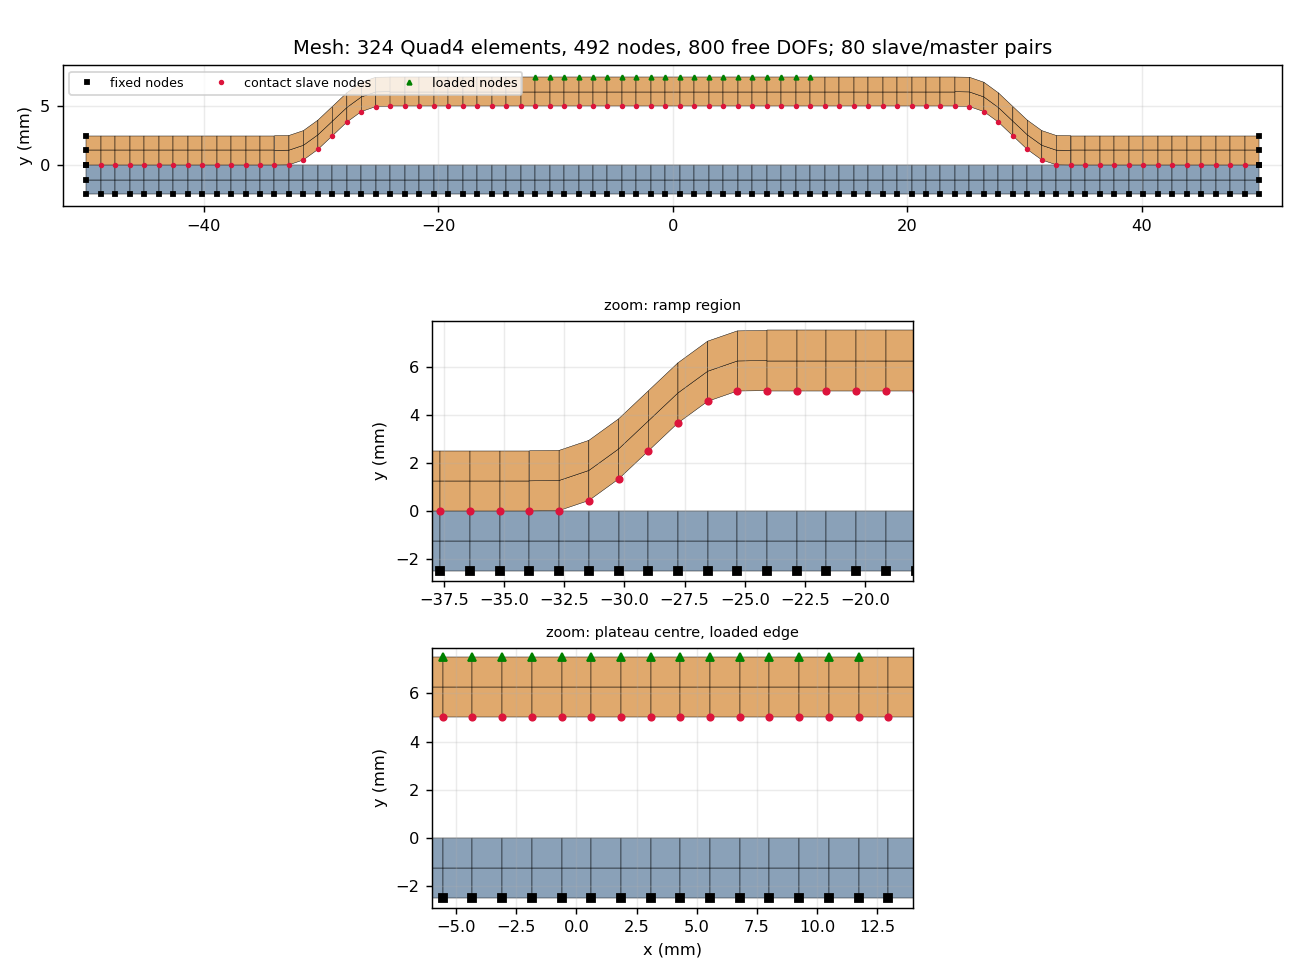
\includegraphics[width=0.95\linewidth]{figures/ch14r/as_mesh.png}
\caption{2D benchmark mesh, 324 elements and 800 free degrees of freedom.}\label{fig:vf-as-mesh}
\end{figure}

\begin{figure}[tbp]
\centering
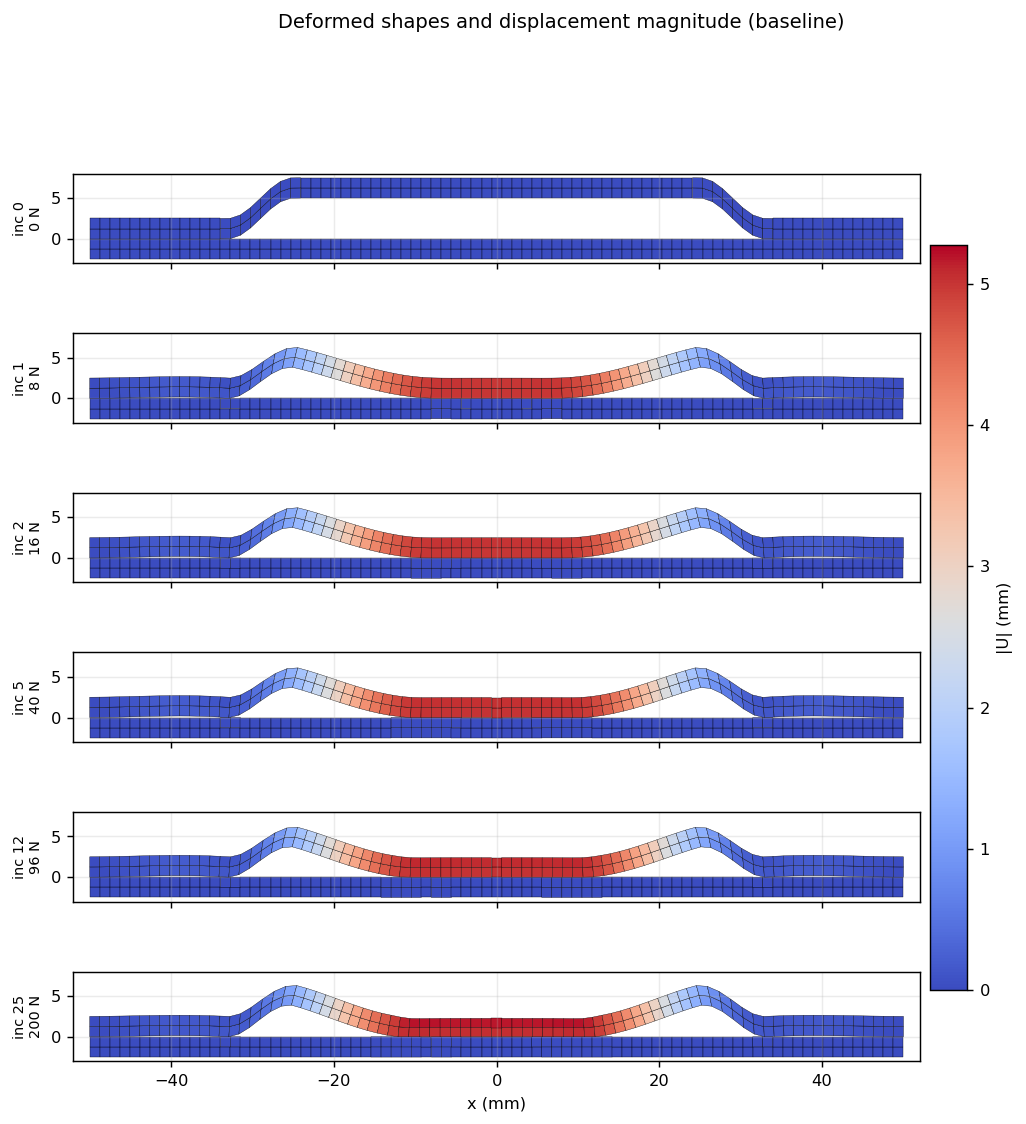
\includegraphics[width=0.95\linewidth]{figures/ch14r/as_baseline_deformed.png}
\caption{Full-order deformed shape of the baseline (as stated) model: contact has already begun in the first increment.}\label{fig:vf-as-defo}
\end{figure}

\subsection*{Results: the 2D benchmark}

\emph{Element and contact onset.} The new element was verified by seven tests. A sensitivity study of 28 variations of the stated parameters (\Cref{fig:vf-as-sens}) shows that the onset of contact is set by the stiffness of the upper part; two single changes, multiplying the Young's modulus of the upper part by 30 or widening the strip to 10~mm, bring the onset into the published window. The study continues with the wider-strip variant, whose singular-value decay is in \Cref{fig:vf-as-svd}. This choice is circumstantial and does not show that the publication used this geometry.

\begin{figure}[tbp]
\centering
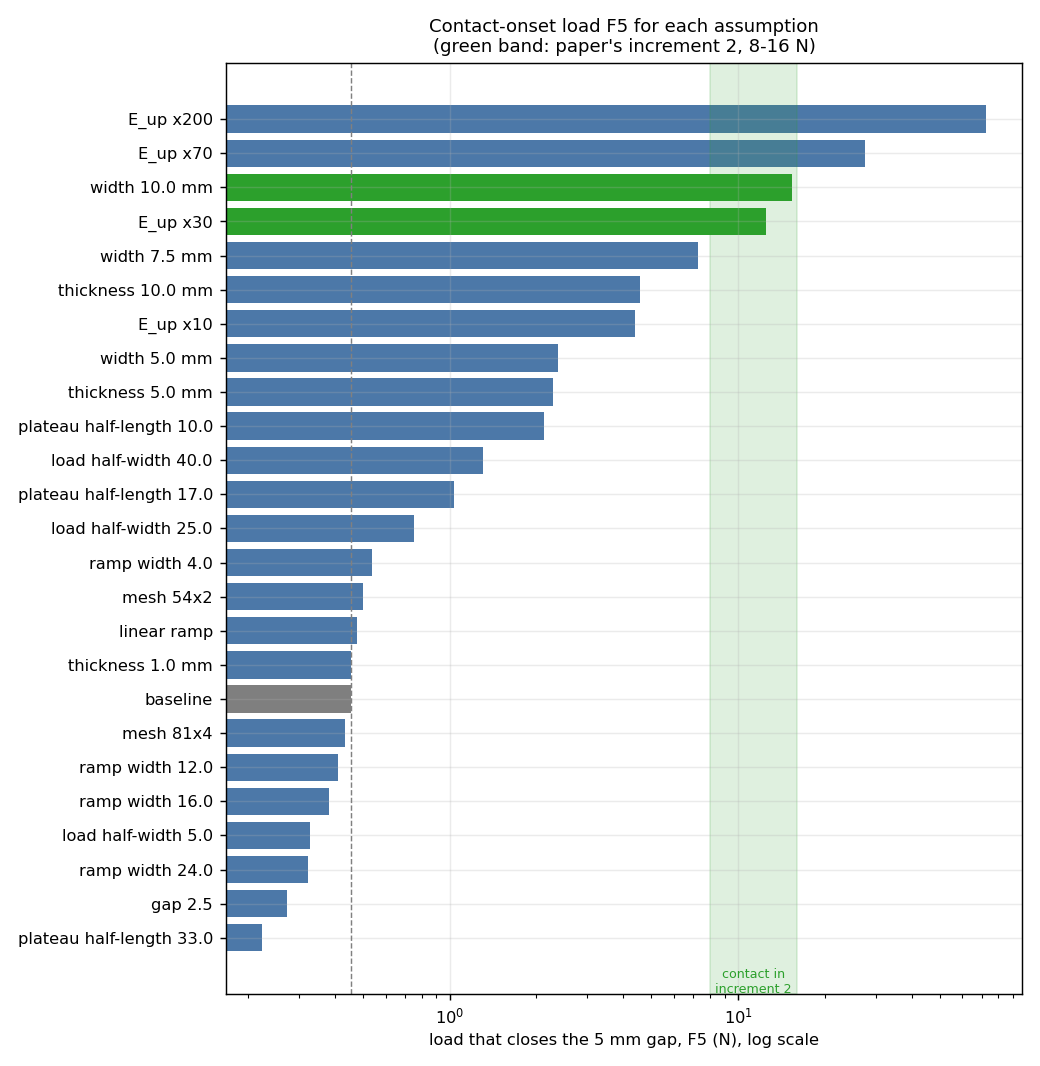
\includegraphics[width=0.85\linewidth]{figures/ch14r/as_sens_bar.png}
\caption{Sensitivity of the contact onset to the 28 parameter variations.}\label{fig:vf-as-sens}
\end{figure}

\begin{figure}[tbp]
\centering
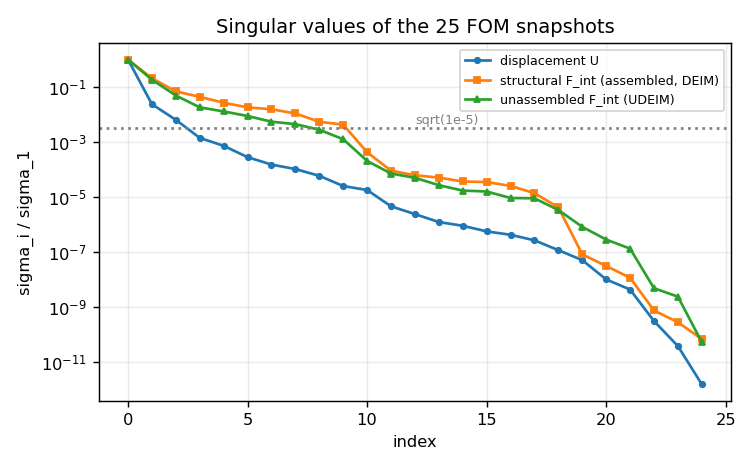
\includegraphics[width=0.8\linewidth]{figures/ch14r/as_width10_svd.png}
\caption{Singular values of the displacement snapshots, 10~mm-wide variant.}\label{fig:vf-as-svd}
\end{figure}

\emph{Plain Newton.} The full-order model needs 86 Newton iterations over the load history (publication 104). The reduced models are in \Cref{tab:vf-as-conv} and \Cref{fig:vf-as-iters}: DEIM and UDEIM fail at $\varepsilon=10^{-6}$ (at increments 2 and 5; publication 18 and 17), POD and ECSW converge, which is the qualitative result of the publication; at $\varepsilon=10^{-9}$ DEIM and UDEIM also converge, which the report could not explain. ECSW was run with $\tau=0.003$ (publication 0.5, which gave no usable model here).

\begin{table}[tbp]
\centering\footnotesize
\caption{2D benchmark with plain Newton (wider-strip variant).}\label{tab:vf-as-conv}
\begin{tabularx}{\linewidth}{@{}>{\raggedright\arraybackslash}p{4.4cm} >{\raggedright\arraybackslash}X >{\raggedright\arraybackslash}X@{}}
\toprule
Quantity & Publication & This work\\
\midrule
Full-order Newton iterations & 104 & 86\\
Failure of DEIM / UDEIM at $\varepsilon=10^{-6}$ & at increments 18 / 17 & at increments 2 / 5; converge at $10^{-9}$\\
POD / DEIM / UDEIM modes & 3 / 11 / 8 & 3 / 10 / 8\\
Error at $\varepsilon=10^{-5}$ & $1.2$--$1.5\,\%$ & $0.94\,\%$\\
Online speed-up POD / DEIM / UDEIM / ECSW & 3.4 / 13.8 / 15.8 / 18.4 & 1.4 / 11.3 / 14.8 / 12.8\\
ECSW tolerance $\tau$ & 0.5 & 0.003\\
\bottomrule
\end{tabularx}
\end{table}

\begin{figure}[tbp]
\centering
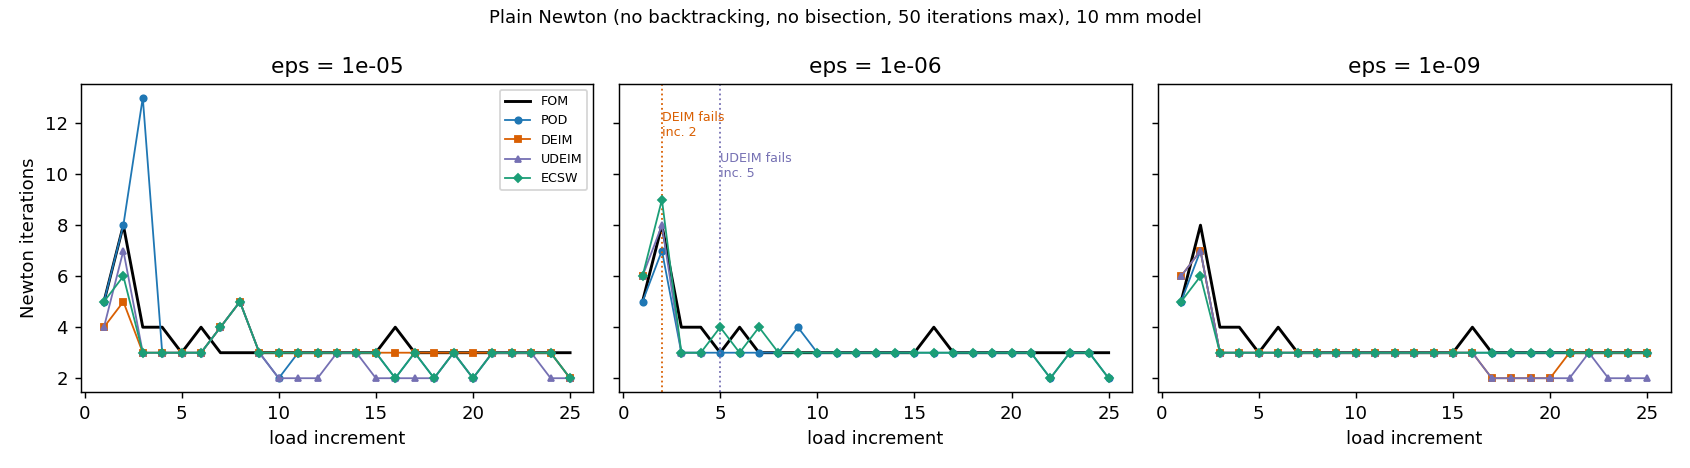
\includegraphics[width=0.85\linewidth]{figures/ch14r/as_rom_iters.png}
\caption{Newton iterations per load increment for the full-order and reduced models.}\label{fig:vf-as-iters}
\end{figure}

\begin{figure}[tbp]
\centering
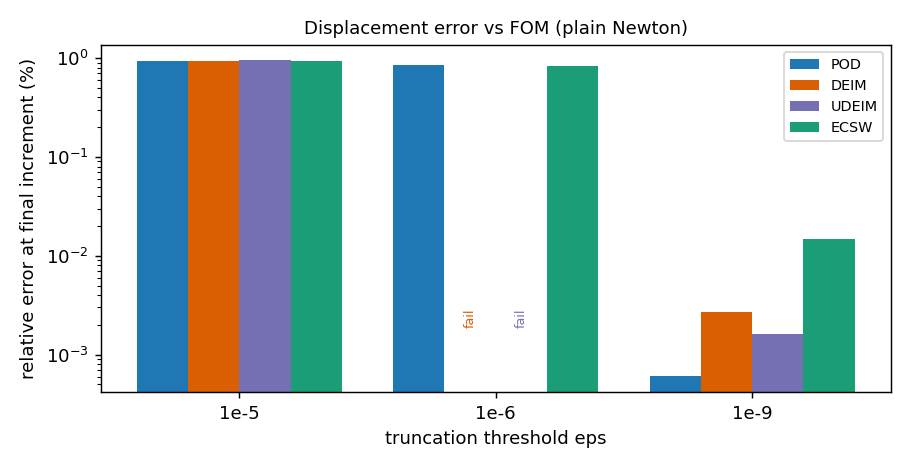
\includegraphics[width=0.85\linewidth]{figures/ch14r/as_rom_errors.png}
\caption{Error of the reduced models against the full-order model at three tolerances.}\label{fig:vf-as-errors}
\end{figure}

\begin{figure}[tbp]
\centering
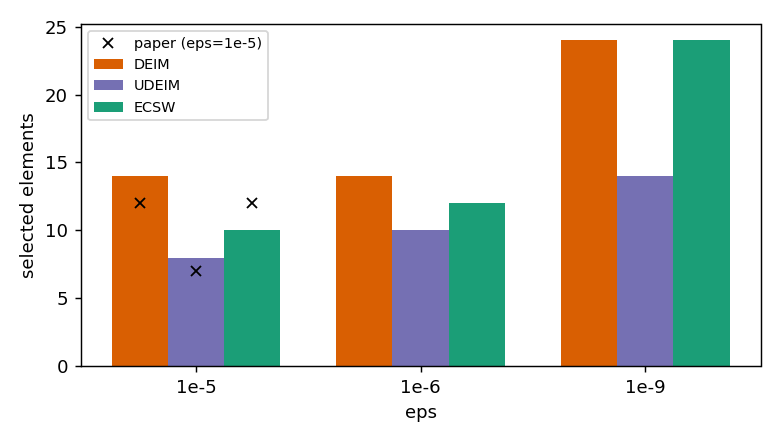
\includegraphics[width=0.85\linewidth]{figures/ch14r/as_rom_elements.png}
\caption{Elements evaluated per iteration against error for the converged runs.}\label{fig:vf-as-elements}
\end{figure}

\begin{figure}[tbp]
\centering
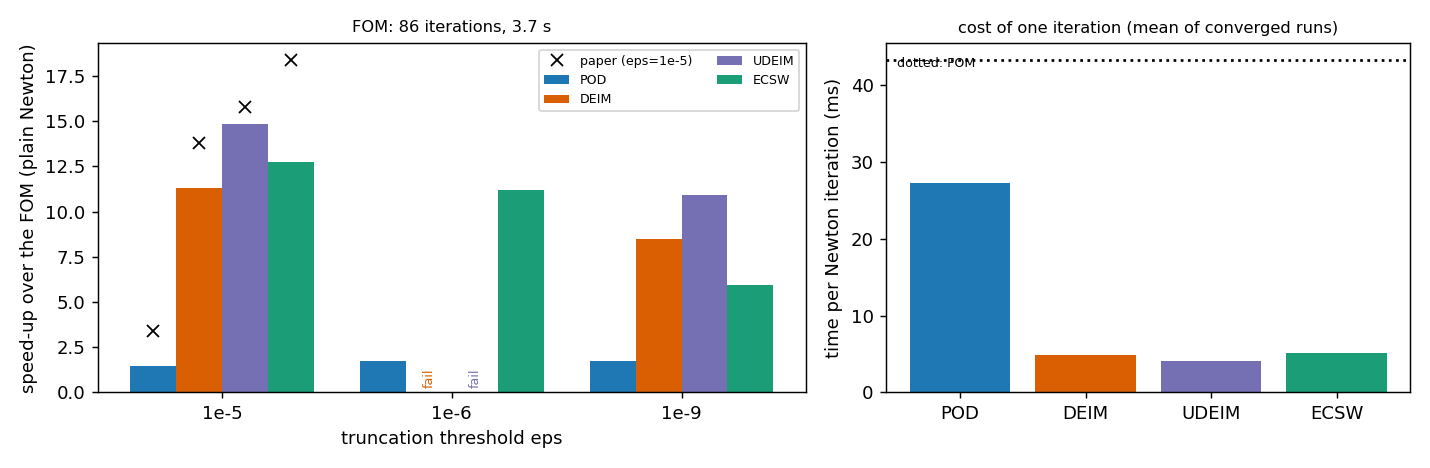
\includegraphics[width=0.85\linewidth]{figures/ch14r/as_timing.png}
\caption{Online timing of the reduced models.}\label{fig:vf-as-timing}
\end{figure}

\begin{figure}[tbp]
\centering
\includegraphics[width=0.95\linewidth]{figures/ch14_asm.pdf}
\caption{2D assembly of \citet{nikiema2026assembly}, plain Newton. (a) Error of the last increment for the four reduced models at three tolerances; crosses mark runs that did not converge (DEIM and UDEIM at $\varepsilon=10^{-6}$). (b) Converged runs: error against the number of elements evaluated per iteration. POD error at $\varepsilon=10^{-5}$: \cvfAsmPodErr.}\label{fig:vf-asm}
\end{figure}

\emph{Domain partitioning.} With the package's indicator at threshold 0.1 the reduced model reproduces the full model to $0.29\,\%$, but 147 to 243 of the 324 elements stay nonlinear, so the speed-up is at most $2.8$ (\Cref{fig:vf-as-dp}, \Cref{fig:vf-as-dptr}). A scan of the number of modes is in \Cref{fig:vf-as-scan}.

\begin{figure}[tbp]
\centering
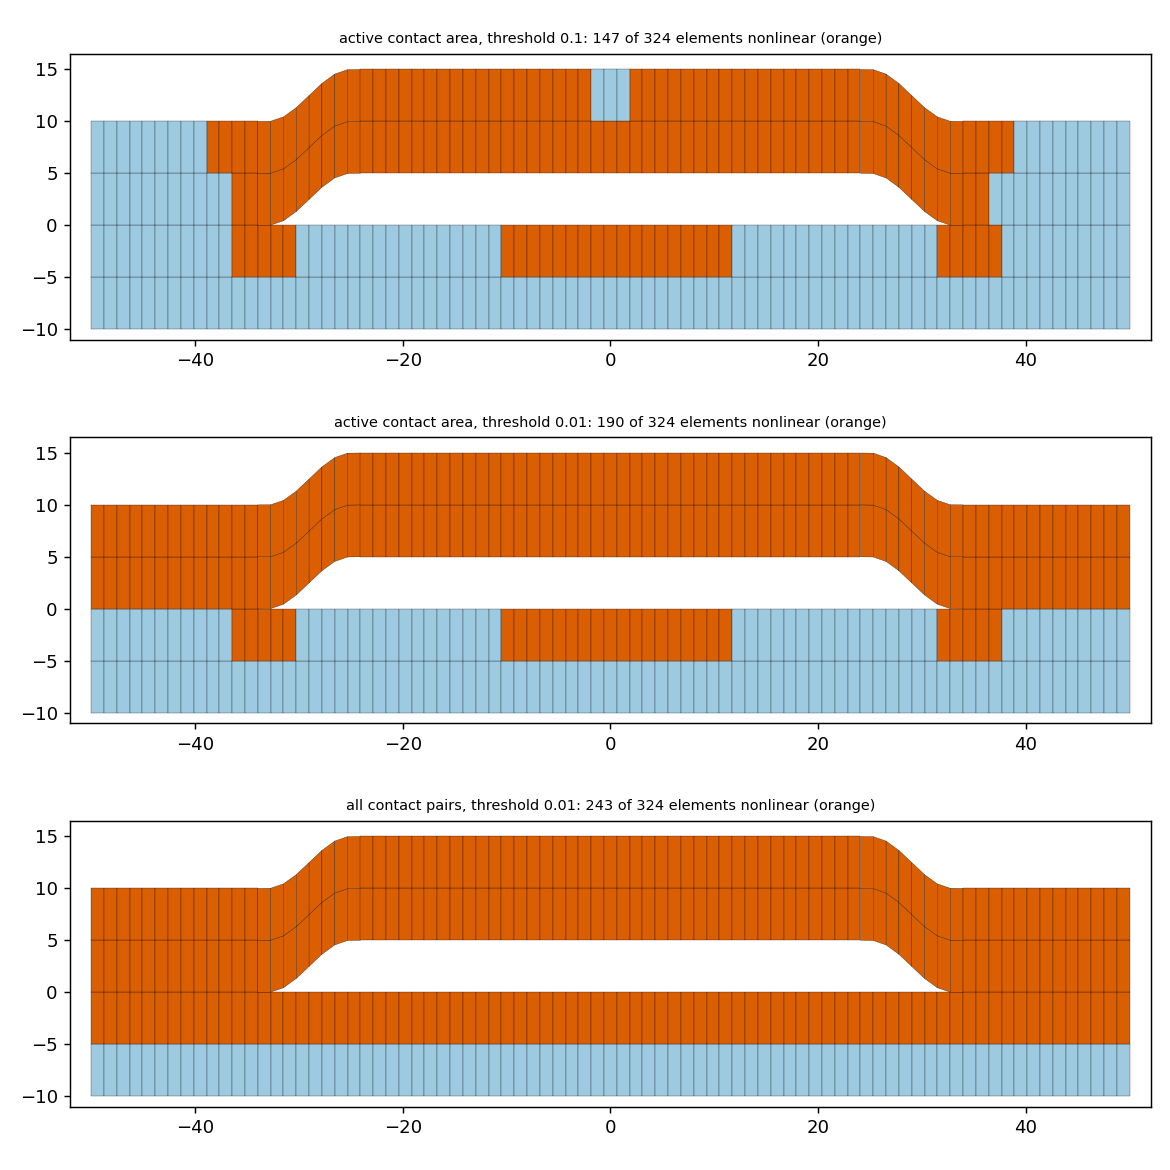
\includegraphics[width=0.85\linewidth]{figures/ch14r/as_dp_zones.png}
\caption{Linear and nonlinear zones from the partitioning indicator.}\label{fig:vf-as-dp}
\end{figure}

\begin{figure}[tbp]
\centering
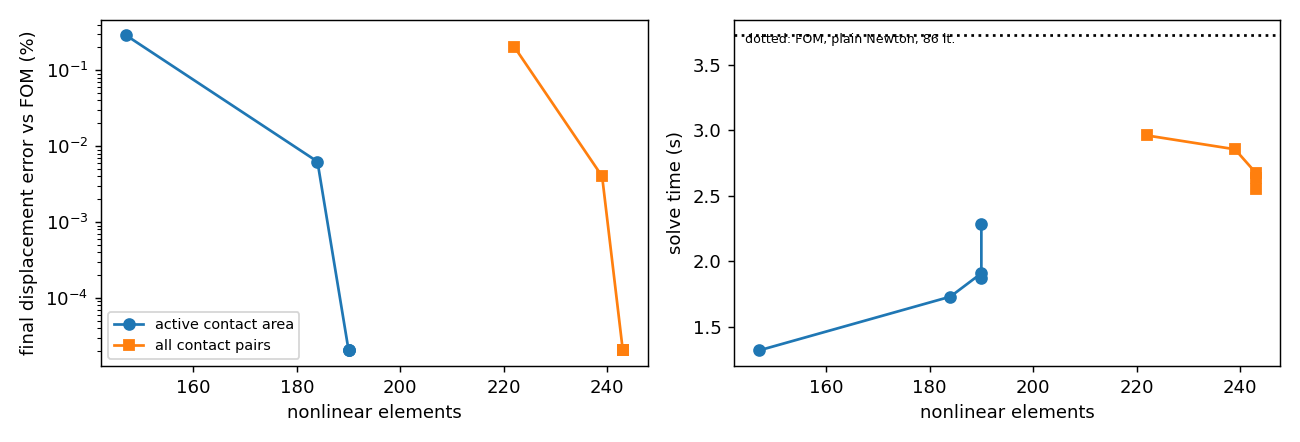
\includegraphics[width=0.85\linewidth]{figures/ch14r/as_dp_tradeoff.png}
\caption{Partitioning: error against speed-up as the threshold varies.}\label{fig:vf-as-dptr}
\end{figure}

\begin{figure}[tbp]
\centering
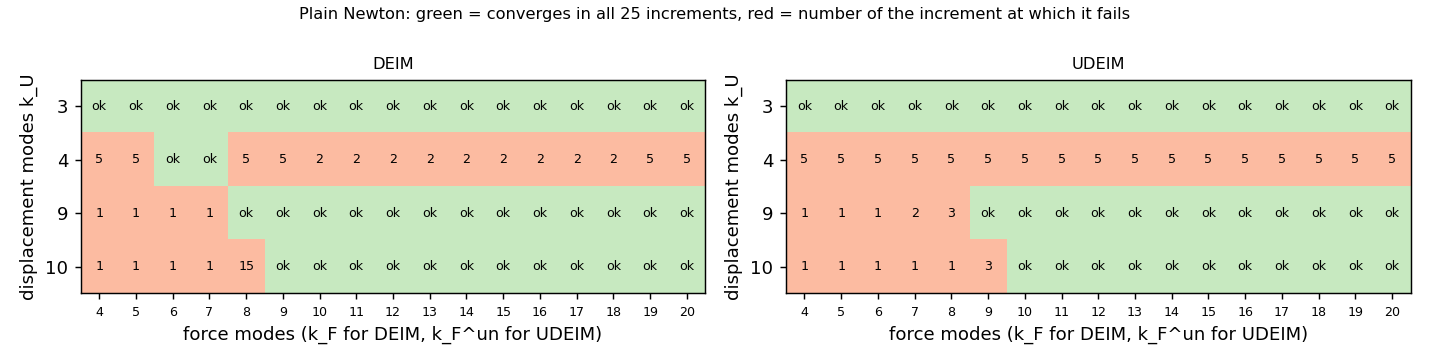
\includegraphics[width=0.85\linewidth]{figures/ch14r/as_mode_scan.png}
\caption{Scan of the number of modes.}\label{fig:vf-as-scan}
\end{figure}

\subsection*{Geometry and mesh: 3D joint}

The 3D pipeline uses total-Lagrangian Hex8 and Hex20 elements (\Cref{fig:vf-as3-el}). Hex8 locks in thin panels, down to $28\,\%$ of the exact bending stiffness, whereas Hex20 gives $0.90$--$0.98$, so Hex20 is used. A scaled butt joint (\Cref{fig:vf-as3-geom}) has 480 Hex20 elements and 12\,087 degrees of freedom. Plain penalty contact made Newton cycle, so a $C^1$-regularised penalty law is used (\Cref{fig:vf-as3-law}); this is a deviation from the publication. The full-order solver uses a symmetric LU factorisation with modified Newton, $3.8\times$ faster than full Newton.

\begin{figure}[tbp]
\centering
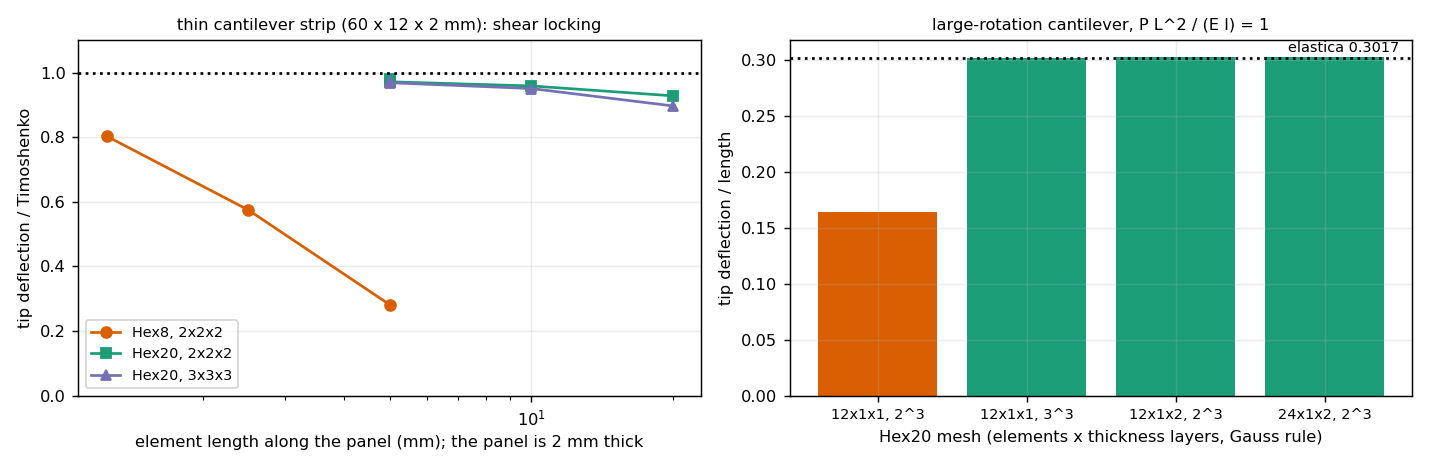
\includegraphics[width=0.7\linewidth]{figures/ch14r/as3_element.png}
\caption{3D elements of the pipeline.}\label{fig:vf-as3-el}
\end{figure}

\begin{figure}[tbp]
\centering
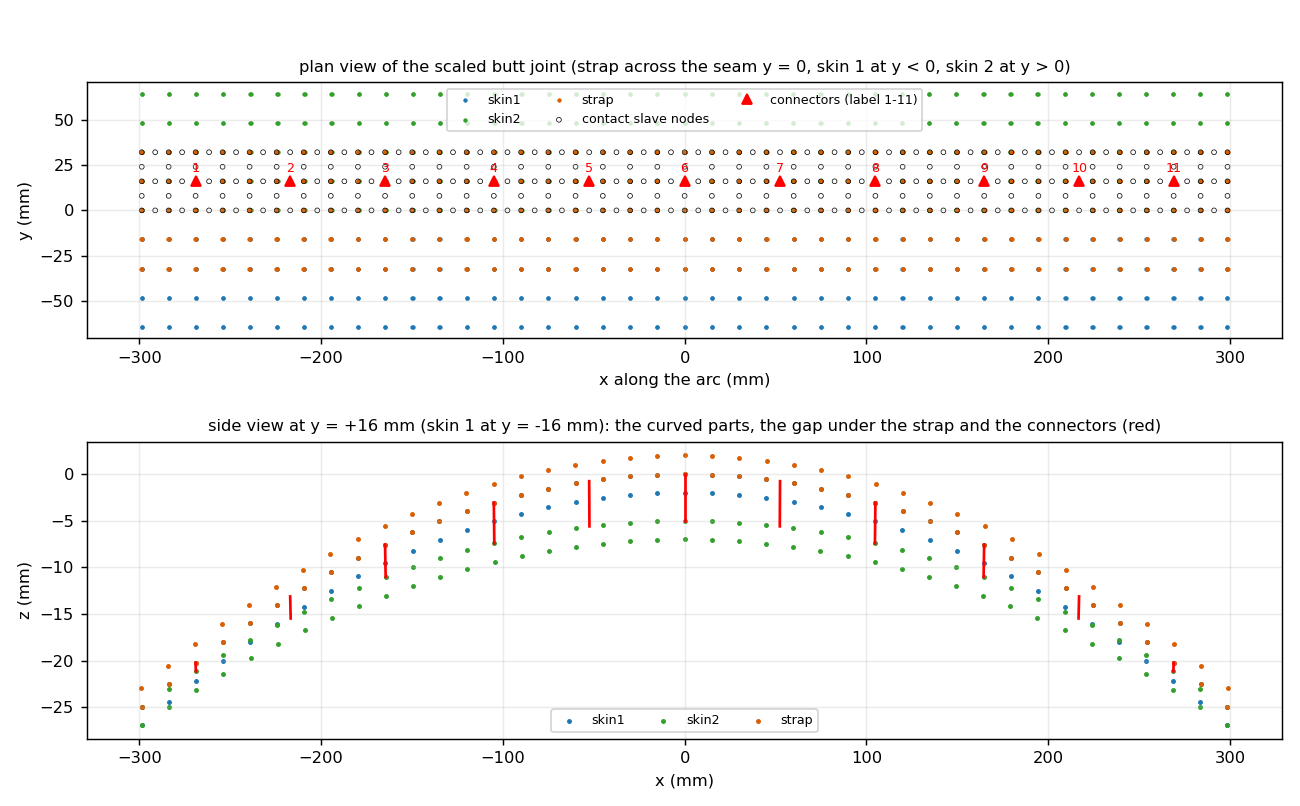
\includegraphics[width=0.95\linewidth]{figures/ch14r/as3_geometry.png}
\caption{Scaled butt joint, 480 Hex20 elements, 12\,087 degrees of freedom.}\label{fig:vf-as3-geom}
\end{figure}

\begin{figure}[tbp]
\centering
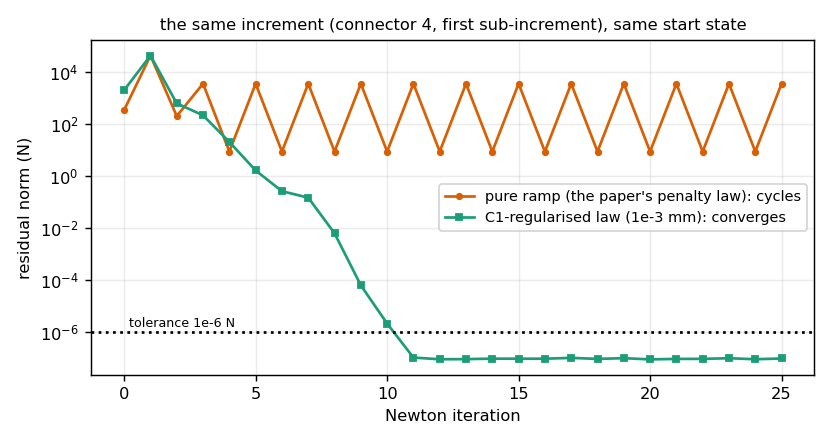
\includegraphics[width=0.7\linewidth]{figures/ch14r/as3_contact_law.png}
\caption{Regularised penalty contact law.}\label{fig:vf-as3-law}
\end{figure}

\subsection*{Results: 3D joint}

With the connectors modelled as rigid (no springs) the nine preload cases of the publication end within $0.3\,\%$ of each other, because the connectors close and the contact absorbs the extra preload, so the benchmark was changed to spring connectors of $k=500$~N/mm, after which the response depends on the preload by $48\,\%$ (\Cref{fig:vf-as3-fom}); the full-order run takes 62~s at 1500~N. \Cref{tab:vf-as3} and \Cref{fig:vf-as3-acc,fig:vf-as3-speed} give the reduced models over nine preloads and four tolerances: POD and ECSW converge in all 36 runs; DEIM and UDEIM as published fail in 34 of 36, because their force approximation is good on training states ($1$--$2\,\%$) and wrong by $10$--$150\,\%$ a short distance off them. The variant that approximates the nonlinear forces including contact (DEIM-NL, UDEIM-NL, an addition of this study, not in the publication) converges in all 36.

\begin{table}[tbp]
\centering\footnotesize
\caption{3D joint with springs: POD error and modes, and speed-up at 1500~N.}\label{tab:vf-as3}
\begin{tabular}{@{}lrrr@{}}
\toprule
 & $\varepsilon=10^{-5}$ & $10^{-6}$ & $10^{-9}$\\
\midrule
POD error (\%) & 1.705 & 0.649 & 0.019\\
POD modes & 20 & 26 & 71\\
Speed-up POD & 1.5 & 1.3 & 1.0\\
Speed-up DEIM-NL & 11.0 & 6.9 & 3.4\\
Speed-up UDEIM-NL & 16.9 & 10.8 & 5.5\\
Speed-up ECSW & 8.8 & 4.3 & 1.4\\
\bottomrule
\end{tabular}
\end{table}

\begin{figure}[tbp]
\centering
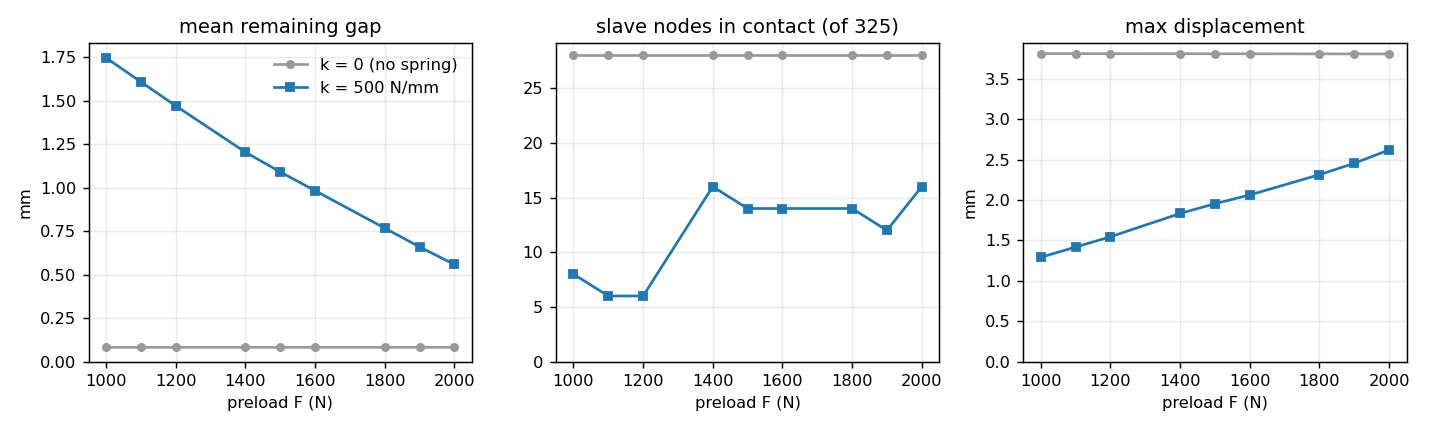
\includegraphics[width=0.85\linewidth]{figures/ch14r/as3_k500_fom.png}
\caption{Full-order response of the spring-connected joint over the nine preloads.}\label{fig:vf-as3-fom}
\end{figure}

\begin{figure}[tbp]
\centering
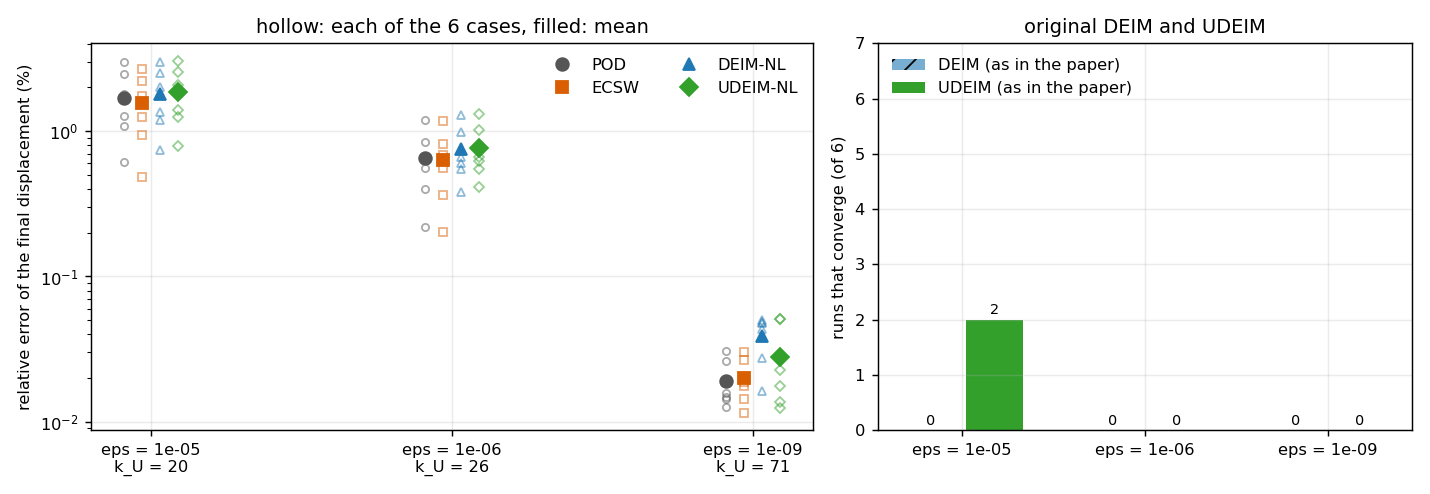
\includegraphics[width=0.85\linewidth]{figures/ch14r/as3_rom_accuracy.png}
\caption{3D joint: accuracy of the reduced models.}\label{fig:vf-as3-acc}
\end{figure}

\begin{figure}[tbp]
\centering
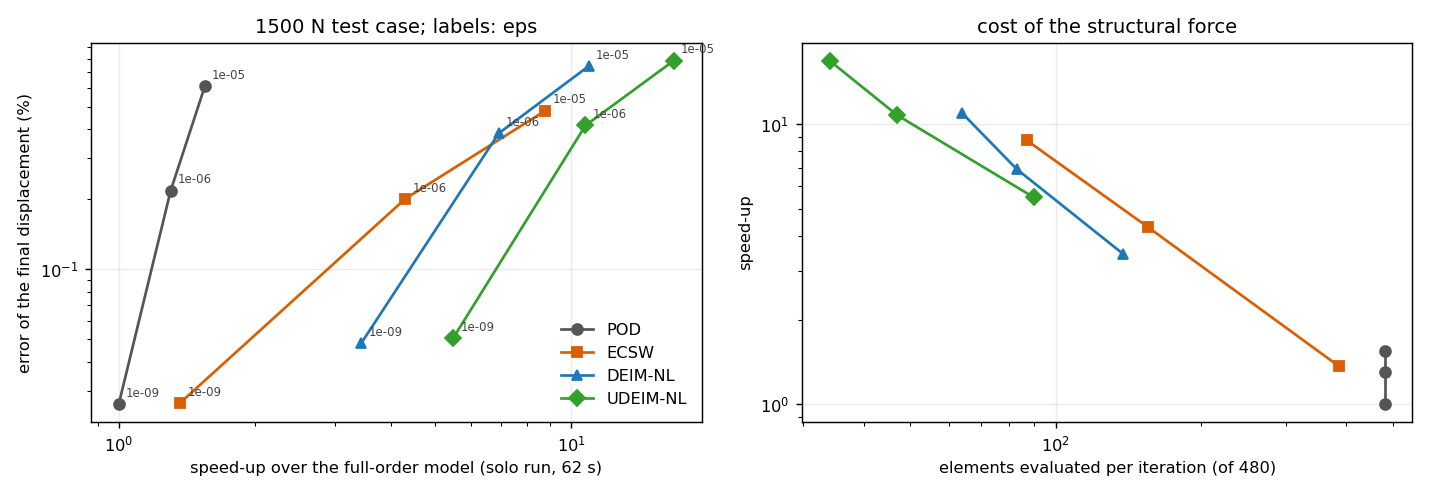
\includegraphics[width=0.85\linewidth]{figures/ch14r/as3_rom_speedup.png}
\caption{3D joint: speed-up of the reduced models.}\label{fig:vf-as3-speed}
\end{figure}

The ECSW speed-up at $10^{-5}$ is $8.8\times$ for 87 of 480 elements, falling to $1.4\times$ at $10^{-9}$, with an offline set-up of 54~s.

\subsection*{Comparison with the publication}

\begin{table}[tbp]
\centering\footnotesize
\caption{Outcome of the reproduction of \citet{nikiema2026assembly}.}\label{tab:vf-as-cmp}
\begin{tabularx}{\linewidth}{@{}>{\raggedright\arraybackslash}p{4.6cm} >{\raggedright\arraybackslash}X >{\raggedright\arraybackslash}p{2.6cm}@{}}
\toprule
Claim & This work & Outcome\\
\midrule
Contact in increment 2 & increment 1 as stated; matched only by changing the geometry & not reproduced as stated\\
DEIM, UDEIM fail with plain Newton; POD, ECSW converge & fail at $10^{-6}$, converge at $10^{-9}$ (2D); fail in 34 of 36 runs (3D) & reproduced, with the $10^{-9}$ exception\\
Mode counts 3 / 11 / 8 & 3 / 10 / 8 & close\\
Error $1.2$--$1.5\,\%$ & $0.94\,\%$ & close\\
Speed-ups 3.4 / 13.8 / 15.8 / 18.4 & 1.4 / 11.3 / 14.8 / 12.8 & lower, same order\\
Domain partitioning saves cost & error $0.29\,\%$, speed-up $\le2.8$ & partly\\
\bottomrule
\end{tabularx}
\end{table}

\subsection*{Where the assembly study departs from the publication}

The publication's geometry is incomplete: with the stated parameters contact begins in the first increment, so the study continues with a variant that is circumstantial. ECSW needed a much smaller tolerance than the stated 0.5. The 3D part is a pipeline and not a reproduction; it uses a regularised contact law, replaces the connectors by springs, covers one parameter (preload) inside the trained range, and the DEIM-NL and UDEIM-NL variants are additions. Not done: other parameters, the publication's full assembly sizes, and an explanation of why DEIM and UDEIM converge at $\varepsilon=10^{-9}$. Each configuration is a single run.

\subsection*{What the reproductions show}\label{sec:vf-repro-summary}

Taken together, the studies show that \fea{} and \rom{} can rebuild nonlinear shell and beam models, train static-condensation, surrogate and contact ROMs on them, integrate those ROMs in time, compute backbones by harmonic balance, identify modal parameters from sparse data, and supply reference fields and frequency-domain ROMs for studies of learned models; and that in several cases the published quantitative claims are recovered within the authors' tolerance. They also show where the reproduced methods reach their limits: a ROM trained on static solves can fail dynamically when in-plane inertia matters or when the training states do not cover the response; a good displacement error can hide a poor contact force; and DEIM-type hyper-reduction can be accurate on training states and wrong a short distance away. They do not show that the packages are faster than other implementations: speed-ups are compared with published numbers only where the publications give them, and the full-order solvers and meshes differ. Where a study could not be reproduced the report says what the publication omits (mesh, damping, thresholds, definition of the error), and those omissions are part of the result.



\section{An integrated parametric pipeline}\label{sec:vf-pipeline}

The studies of the previous section test methods against other people's numbers. This section tests the book's own stack against itself, end to end, in the way a user would build a parametric model: a mesh from the generators, a system from \fea{}, snapshots, a basis, an affine reduced model from \rom{}, and then queries at parameters \emph{and} loads that no earlier step saw, reported by the convention of Appendix~\ref{ch:conv}. Everything in this section was produced in the setup named in \Cref{tab:vf-pipeline}, in one run each for the two meshes, and the timings are single runs (minimum over repeats of the loop in question), which vary by tens of percent between runs.

\paragraph{The model.}
A cantilever plate of $0.4\times0.2$~m and thickness $0.02$~m in plane stress is built as two blocks (left and right half) with Young's moduli $E_1$ and $E_2$ in $[0.5,2.5]\times10^{11}$~Pa as the two parameters. The stiffness is affine, $\bm K(\bm\mu)=E_1\bm K_1+E_2\bm K_2$, with $\bm K_q$ assembled once with a unit modulus in one block and zero in the other. The load is a traction on the free edge. Two meshes are used: a small one of \cplSElems{} Quad4 elements (\cplSFree{} free dofs) and a larger one of \cplLElems{} elements (\cplLFree{} free dofs); the larger one is the largest that fits the memory of the reference setup, because \anchor{rom_engine.affine.AffineDecomposition} takes its component matrices as dense arrays and a sparse matrix is rejected.

\tikzfigure[0.98\linewidth]{ch14_workflow}{The integrated pipeline. Blue: \fea{}; violet: \rom{}; grey: data; green: checks. The basis size is chosen on a validation set of the training kind; the two test sets are used once, at the end.}{fig:vf-workflow}

\begin{algbox}{Integrated parametric pipeline with loads not used in training}
\begin{pseudo}
\Require mesh generator, parameter range, eight polynomial traction shapes $\bm s_1,\dots,\bm s_8$, number of training pairs $N$, tolerance tol
\State build the two-block system; assemble $\bm K_1,\bm K_2$ (unit moduli) and restrict them to the free dofs
\State draw $N$ parameters $\bm\mu_i$ by Latin hypercube and loads $\bm f_i=\sum_j c_{ij}\bm s_j$ with random $c_{ij}$
\State solve $\bm K(\bm\mu_i)\bm u_i=\bm f_i$ for all $i$;\ POD of $[\bm u_1\ \cdots\ \bm u_N]$ $\to\bm V$ \Comment{offline}
\State $\bm K_{r,q}\gets\bm V^T\bm K_q\bm V$ for $q=1,2$ \Comment{offline, once}
\For{$r$ in the grid of basis sizes}
  \State on the validation set (new $\bm\mu$, loads of the training kind): errors of the full state and of the four local quantities
\EndFor
\State $r^\ast\gets$ smallest $r$ whose largest validation error is at most tol
\For{each query $(\bm\mu,\bm f)$ of the test sets}
  \State $\bm q\gets(\sum_qE_q\bm K_{r,q})^{-1}\bm V_{r^\ast}^T\bm f$;\ $\bm u\gets\bm V_{r^\ast}\bm q$ \Comment{online, then lift}
  \State tip deflection, peak von Mises stress, total reaction and root moment from $\bm u$ \Comment{recovery: the same code as for the full model}
  \State residual indicator $\|\bm f-\bm K(\bm\mu)\bm u\|/\|\bm f\|$
\EndFor
\State report: errors against the full model on both test sets, offline, online, lift and recovery cost, break-even number of queries
\Ensure reduced model and its report
\end{pseudo}
\end{algbox}

Offline the cost is $N$ full-order solves, one SVD of an $n\times N$ matrix and two small projections; online each query costs one $r\times r$ solve, one lift, and the recovery of the local quantities, which costs the same as for the full model. The pipeline breaks when the loads of the queries are not in the span the training loads explored (the error stops falling with $r$, \Cref{fig:vf-pipeline}a), when the parameter range is left, or when the local quantity of interest depends on the field in a way the basis does not carry. The code is \anchor{fea_engine.solver.FESystem}, \anchor{rom_engine.pod.PodBasis} and \anchor{rom_engine.affine.AffineDecomposition}; \Cref{tab:vf-pl-err}, \Cref{tab:vf-pipeline} and \Cref{fig:vf-pipeline} are the checks.

\paragraph{Training, validation, tests.}
\cplSNtrain{} training pairs are drawn, each with a different parameter and a different random mixture of the eight traction shapes ($x$- and $y$-tractions of degrees 0 to 3 in the coordinate along the edge). The basis size is chosen on a separate validation set of 20 queries of the same kind: the smallest $r$ for which the largest error of the full state and of the four local quantities is at most $10^{-3}$; both meshes give $r=\cplSR$ (the criterion is \cplSSelMet{} on the small mesh and \cplLSelMet{} on the large one). Two test sets of 40 queries each are then evaluated once. Set~A has new parameters and loads of the training kind (new random mixtures). Set~B has new parameters and a load shape outside the span of the training shapes, a vertical traction $a\sin\pi y$ with $a$ of random sign and size. The local quantities are the tip deflection, the peak von Mises stress, the total vertical reaction and the root moment about the out-of-plane axis; the last two are computed from the reaction forces $\bm K\bm u$ at the clamped dofs and are compared with the load scale and not with their own value, because a resultant can cancel for a load of mixed sign.

\begin{table}[tbp]
\centering\small
\caption{Errors on queries not used in training at $r=\cplSR$ (largest over the 40 queries of each test set). The two local quantities in the lower rows are relative to the load scale.}\label{tab:vf-pl-err}
\begin{tabular}{@{}l rr rr@{}}
\toprule
 & \multicolumn{2}{c}{small mesh (\cplSFree{} dofs)} & \multicolumn{2}{c}{large mesh (\cplLFree{} dofs)} \\
\cmidrule(lr){2-3}\cmidrule(lr){4-5}
 & set A & set B & set A & set B \\
\midrule
full state (relative $\ell_2$) & \cplSAGlob & \cplSBGlob & \cplLAGlob & \cplLBGlob \\
tip deflection & \cplSATip & \cplSBTip & \cplLATip & \cplLBTip \\
peak von Mises stress & \cplSAVm & \cplSBVm & \cplLAVm & \cplLBVm \\
total vertical reaction & \cplSARy & \cplSBRy & \cplLARy & \cplLBRy \\
root moment & \cplSAMz & \cplSBMz & \cplLAMz & \cplLBMz \\
\bottomrule
\end{tabular}
\end{table}

\begin{figure}[tbp]
\centering
\includegraphics[width=\linewidth]{figures/ch14_pipeline.pdf}
\caption{(a) Largest error against the basis size $r$ on the validation set and the two test sets (small mesh): the full state, and for set~B also the peak stress; the horizontal line is the tolerance and the vertical line the chosen $r$. (b) Online residual indicator against the true error of the full state for the 80 test queries. (c) Time per query on the small mesh.}\label{fig:vf-pipeline}
\end{figure}

\paragraph{What the errors say.}
Every error of \Cref{tab:vf-pl-err} is below $10^{-3}$ on both meshes, and parameters and loads not used in training cause no larger error than the validation set did, so in this problem the selection on validation data transfers to the tests. Three observations qualify that. First, the full-state error of set~B does not keep falling with $r$: it stops near \cplBFloor{} beyond $r\approx16$ (\Cref{fig:vf-pipeline}a), while set~A falls to \cplAFloor{} at $r=24$. The sine load is not in the span of the polynomial traction shapes, so a part of it cannot be represented by any basis built from them, however large; a load outside the training span sets a floor on the error that the number of modes cannot lower. Second, the local errors are not ordered like the global one: for set~A the error of the total reaction is \cplSARy{} against \cplSAGlob{} for the full state on the small mesh, and on the large mesh the reaction and the peak stress are above the tip deflection by a factor of two to five. A local quantity that is a derivative of the field (a stress) or an integral of it (a reaction) depends on parts of the field that the global norm weights little, which is why Appendix~\ref{ch:conv} asks for one next to the other. Third, the cheap online indicator, the relative residual of the full equation, tracks the error across the two sets (Spearman correlation \cplSpearman), but within set~B, whose residual is nearly constant (\cplResidB) because it is dominated by the part of the load the basis cannot carry, the correlation is only \cplSpearmanB. The indicator is a screening tool, not a bound, and it says nothing about which part of a residual is representable.

\begin{table}[tbp]
\centering\small
\caption{Cost of the pipeline by the convention of Appendix~\ref{ch:conv}: offline, online, lift and recovery separately, two full-order baselines, and the break-even number of queries (offline cost divided by the saving per query, the lift included). Software: NumPy 2.2.6. Single runs; times vary by tens of percent between runs.}\label{tab:vf-pipeline}
\begin{tabular}{@{}lrr@{}}
\toprule
 & small mesh & large mesh \\
\midrule
free dofs & 624 & 4\,224 \\
elements & 288 & 2\,048 \\
basis size $r$ & 16 & 16 \\
\midrule
offline: 24 snapshot solves (ms) & 63.2 & 1\,126 \\
offline: POD (ms) & 0.731 & 4.23 \\
offline: projection (ms) & 10.6 & 219 \\
offline: total (ms) & 74.5 & 1\,349 \\
\midrule
FOM re-assembled + sparse solve (ms/query) & 332 & 2\,765 \\
FOM sparse affine + solve (ms/query) & 2.52 & 42.9 \\
ROM online solve (ms/query) & 0.0251 & 0.0477 \\
ROM lift to full space (ms/query) & 0.00506 & 0.0287 \\
stress recovery, either model (ms/query) & 3.34 & 15.1 \\
residual indicator (ms/query) & 0.212 & 0.568 \\
\midrule
break-even queries, against re-assembled FOM & 0.225 & 0.488 \\
break-even queries, against sparse affine FOM & 29.9 & 31.5 \\
\bottomrule
\end{tabular}

\end{table}

\paragraph{Cost.}
The offline cost on the small mesh is \cplSOff~ms, of which \cplSOffSnap~ms are the $\cplSNtrain$ snapshot solves. Against a full-order baseline that re-assembles the stiffness for every query through \code{assemble_stiffness}, which takes \cplSTFomreasm~ms in the Python element loop on the small mesh, the reduced model pays for itself before the first query (break-even \cplSBeReasm{} queries). That baseline is the one a user who changes the material and calls the engine again would have, but it is a poor one: the stiffness is affine, so a full-order solver that forms $E_1\bm K_1+E_2\bm K_2$ and solves it sparsely takes \cplSTFomsparse~ms (\cplLTFomsparse~ms on the large mesh), against \cplSTRom~ms for the reduced solve. Against that baseline the break-even is \cplSBeSparse{} queries on the small mesh and \cplLBeSparse{} on the large one, and the online solve alone is faster by a factor of \cplSSpeedSparse{} and \cplLSpeedSparse. The workflow, however, does not end at the solve. Recovering the local quantities from the lifted field costs \cplSTRecover~ms on the small mesh and \cplLTRecover~ms on the large one, more than a hundred times the reduced solve, and the full-order workflow pays the same: the ratio of the two complete workflows, recovery included, is \cplSSpeedFlowSparse{} on the small mesh and \cplLSpeedFlowSparse{} on the large one against the sparse affine baseline (and \cplSSpeedFlowReasm{} and \cplLSpeedFlowReasm{} against the re-assembled one). A speed-up of the online solve alone, such as those quoted for reduced models in the literature and in the previous section, is therefore not a speed-up of the workflow whenever the answer of interest is a stress or a reaction. A reduced model that recovers stresses only at the few elements of interest, or a hyper-reduced recovery, would change this ratio; none of them is part of the pipeline above.

\begin{sidenote}{Speed-up and break-even}
The \emph{speed-up} of a reduced model is the time of a full-order query divided by the time of a reduced one. It says nothing about the cost of building the model. The \emph{break-even} number of queries is the offline cost divided by the saving per query, and below it the reduced model is a net loss. Speed-ups depend on the implementation and on the machine, so they are reported with both.
\end{sidenote}

\subsection{The speed-up discrepancy}\label{sec:vf-speed}
Three different speed-ups of the two-region beam example have been quoted for this stack: $221.8$ in the README and the user guide (a 500-point sweep, $1653.23$~ms against $7.45$~ms, no machine stated), $361$ in the measurements supplied with the article (the same beam, $242$ dofs, $3.646$~s against $10.1$~ms, minimum over repeats of the whole sweep, commit 33cde35), and $254$ in an earlier manuscript. A search of the repository and of the article finds $254$ nowhere, and this book does not quote it. The example script of the repository was run \cplRdRuns{} times in the reference setup of this book: the full-order sweep of $500$ queries (stiffness re-assembly and a dense solve) takes about \cplRdFomMs~ms and the reduced one about \cplRdRomMs~ms, and the ratio is between \cplRdMin{} and \cplRdMax{} (median \cplRdMed). The README value lies inside that range, and so would any figure within about fifteen per cent of it: the reduced sweep takes only about ten milliseconds, so a change of one millisecond moves the ratio by ten per cent. The measurements of the article differ for a second reason as well, because they take the minimum over repeats and not a single pass. The three numbers are therefore not in conflict and none is a property of the code: each is a ratio of two timings on one system under one timing rule, with a dense full-order baseline (\Cref{ch:pod}), and the book quotes only the ratio it generated, together with its range.

\section{Limits of this chapter}\label{sec:vf-limits}

\begin{limitsbox}
\begin{itemize}
\item \textbf{One author, one setup.} The reproductions were written and run by the author of the packages. They show that the packages can rebuild a method from its description; they are not an independent confirmation, and the choices a publication leaves open were filled by the person who wrote the code.
\item \textbf{The reports were not re-run at the tag.} The figures are redrawn from saved outputs of the study folders, with caption numbers computed from them and compared with the written reports; the studies themselves (\texttt{--rerun}) were not repeated at \booktag{}, and their drivers live outside the repository.
\item \textbf{Small models, single runs.} Most studies use meshes of a few hundred to a few tens of thousands of degrees of freedom, speed-ups are against full-order solvers that differ from the publications', timings vary by tens of percent, and the network studies use one seed per configuration. No statement about large industrial models follows, and differences inside that noise are not findings.
\item \textbf{The pipeline is a plate with two materials.} It tests one parameter pair, one basis size chosen on a validation set, and loads inside and outside the trained span (the latter sets an error floor of about $1.7\times10^{-4}$). Geometry or topology changes, nonlinearity and a hyper-reduced recovery are not tested, the package's affine decomposition accepts dense components only, and the residual indicator ranks queries but is not a bound.
\item \textbf{Open items.} The fluid-structure study has no redrawn figure, the network trainings need PyTorch and a GPU that this book's build did not have, and the modal frequencies quoted for the first reproduction (79/218/427/706~Hz in the publication) are not all retained in the saved data.
\end{itemize}
\end{limitsbox}

\section{Summary}\label{sec:vf-summary}

We began by asking what a number in this book proves. The answer is a ladder of six levels, from a unit test to an integrated run, where each level answers a different question and a higher one does not replace a lower one. The component checks of Chapters~\ref{ch:elem} to~\ref{ch:hyper} establish that the parts do what the mathematics says on cases with a known answer.

The nine reproductions show that published studies could be rebuilt from the packages, and their outcomes are recorded as they came, including the failures: the dynamic accuracy of statically trained ROMs, contact forces hidden behind good displacements, and DEIM-type hyper-reduction going wrong a short distance from its training states. The integrated pipeline then followed one model from mesh to loads not used in training, with offline, online, lift and recovery cost separated. In it, stress recovery and not the reduced solve dominated the workflow, so a speed-up of the solve alone is not a speed-up of the answer; and the three speed-ups quoted for the example beam are single timings under different rules, none of them a property of the code.

\section*{Exercises}\label{sec:vf-exercises}

\begin{enumerate}
\item \emph{(Derivation)} The break-even number of queries is the offline cost divided by the saving per query, lift included. Derive it, and show that if recovery costs the same in the full-order and the reduced workflow, the workflow speed-up is smaller than the speed-up of the solve alone and tends to $1$ as recovery dominates.
\item \emph{(Derivation)} A reduced model has a maximum error of $10^{-4}$ on training loads and a floor of $1.7\times10^{-4}$ for a load outside their span. Explain, with the decomposition of the load into a component in the span and one orthogonal to it, why increasing $r$ cannot lower the floor.
\item \emph{(Implementation)} Run the pipeline of this section with a different validation set and a different candidate list of $r$. Report the chosen $r$ and the errors by the convention of Appendix~\ref{ch:conv}.
\item \emph{(Implementation)} Replace the dense affine components of the pipeline by sparse ones. Find where \code{AffineDecomposition} refuses them, and give the smallest change that would accept them.
\item \emph{(Implementation)} Add a recovery of stress at 20 elements only and measure the workflow speed-up again. State what changes in the break-even number.
\item \emph{(Interpretation)} The ICE ROM of Section~\ref{sec:vf-ice} fits the static modal force with $R^2=0.9998$ and still fails under random loading. Which level of Figure~\ref{fig:vf-pyramid} would have caught this, and what test would you add at the level below it?
\item \emph{(Interpretation)} A reproduction matches a published error to two digits. List three reasons this may not confirm the method, using the open inputs recorded in Section~\ref{sec:vf-asm}.
\item \emph{(Interpretation)} Read the speed-up discrepancy of Section~\ref{sec:vf-speed}. Specify a timing protocol (repeats, statistic, machine report) under which a single number could be quoted, and say what it would still not show.
\end{enumerate}

\chapterrefs


\appendix
\chapter{Differentiable assembly and autograd tangents}\label{ch:diff}

\begin{tcolorbox}[colback=gray!5,colframe=gray!50,title={In this appendix}]
Several places in the book need a derivative of a function that is only available as code: the tangent stiffness of an element whose force routine is known but whose consistent tangent is intricate (Chapters~\ref{ch:elem} and~\ref{ch:nonlin}), and the gradient of a quantity of interest with respect to the parameters of a model that is solved by Newton's method. This appendix describes the optional PyTorch layer of the two packages that supplies both. It has three parts: exact element tangents by automatic differentiation, used as an independent check of the tangents that the elements compute by other means; a trainable additive correction of the nonlinear static residual with an explicit and an implicit way to calibrate it; and a reduced-coordinate counterpart of the correction in \rom{}. Everything that does not need PyTorch is run in this book; what does is quoted from the tests and says so.
\textbf{After this appendix the reader can:} (i) say what a tangent computed by automatic differentiation is exact for, and what a central difference loses; (ii) write the residual, the Newton tangent and the gradient for a corrected static problem; (iii) differentiate through a converged Newton solve with one adjoint solve instead of unrolling the iteration; (iv) choose between explicit and implicit calibration; (v) read the verification of this layer for what was run and what was not.
\end{tcolorbox}

\section{Three uses of a derivative}\label{sec:df-uses}

The force routine of an element, $\bm f_e(\bm u_e)$, is usually the first thing written, because it follows from the virtual work of a strain energy. The tangent $\bm K_e=\partial\bm f_e/\partial\bm u_e$ then has to be consistent with it, or Newton's method loses its quadratic rate. Three situations call for a derivative that the force routine does not give for free.

\emph{An element tangent.} For the compressible neo-Hookean tetrahedron, \anchor{fea_engine.elements.nonlinear_solids.Tet4NeoHookean} computes the tangent by central differences of its closed-form force; for the shell with a committed state, \anchor{fea_engine.elements.shells.Shell4MITCCorotational} uses the complex-step derivative~\cite{squire1998complex}. A third method that is exact and independent of both is a check on the force law and on the tangent at once.

\emph{A gradient through a solve.} If the load, a material parameter or a correction term is to be fitted so that a displacement matches a measurement, one needs $\mathrm dL/\mathrm d\bm\theta$ for a loss $L$ of the converged state $\bm u^\ast(\bm\theta)$. Differentiating the Newton iteration step by step is possible but stores every iterate and ties the cost to the iteration count~\cite{griewank2008evaluating}.

\emph{A trainable correction.} The residual of a model can be completed by a term with free parameters, $\bm f_\theta$, which is then fitted to reference data. This is the setting of the method of Saverio and co-authors~\cite{saverio2026endtoend}, who correct a turbulence model of a flow solver inside the solve; the packages carry the same construction over to the residual of a nonlinear structure.

The layer is optional. PyTorch~\cite{paszke2019pytorch} is imported inside a guard, importing the modules never needs it, and every function that does need it raises an error that says so. The mathematical content of the correction (the corrected Newton solve, the adjoint formula, the metric identity) is written against a plain \code{value()}/\code{jacobian()} protocol and runs on NumPy alone; that is what lets this appendix run it.

\section{Mathematical structure}\label{sec:df-math}

\subsection{Tangents: three ways to a derivative}\label{sec:df-tangent}

Let $\bm f:\mathbb R^n\to\mathbb R^n$ be the force of an element and $\bm e_j$ the $j$th unit vector. A central difference, $(\bm f(\bm u+h\bm e_j)-\bm f(\bm u-h\bm e_j))/2h$, has a truncation error of order $h^2$ and a rounding error of order $\varepsilon_{\mathrm{mach}}/h$, so that its error is smallest near $h\sim\varepsilon_{\mathrm{mach}}^{1/3}\approx6\times10^{-6}$ and cannot be made smaller by choosing $h$ well; the constant in front depends on the third derivative of $\bm f$ and on its size. The complex-step formula, $\mathrm{Im}\,\bm f(\bm u+\mathrm i h\bm e_j)/h$, has no subtraction and can use $h=10^{-30}$, but it needs the force routine to be analytic in its arguments and to be written for complex numbers. Reverse-mode automatic differentiation records the operations of one evaluation of $\bm f$ and returns a row of $\bm K$ per backward pass, $\partial f_i/\partial\bm u$, to rounding error, with no step size and for any routine written with differentiable operations. A full $n\times n$ element tangent therefore costs $n$ backward passes after one forward pass; for many elements of the same type the passes can be batched over the elements (\anchor{fea_engine.autograd_tangent.tet4_neo_hookean_tangent_autograd_batched}).

An exact derivative of a force that is the gradient of a scalar energy is symmetric to rounding. For the neo-Hookean tetrahedron the autograd tangent is deliberately not symmetrised, so that an asymmetry would be visible as a defect. The shell with a committed state is different: its force is not the gradient of a potential, so its true Jacobian is asymmetric, the package returns the symmetrised matrix by convention, and the check below compares symmetrised matrices.

\subsection{A trainable additive correction}\label{sec:df-corr}

The static residual of the package is $\bm R(\bm u)=\bm F_{ext}-\bm F_{int}(\bm u)$. The correction enters as a further internal force, with free parameters $\bm\theta$,
\begin{equation}\label{eq:df-res}
\bm R_\theta(\bm u)=\bm F_{ext}-\bm F_{int}(\bm u)-\bm f_\theta(\bm u)=\bm 0 .
\end{equation}
The sign is the one of the package, in which the internal force carries the minus sign; the source writes the same term with the opposite sign because its operator is the negative of ours. Newton's method on \eqref{eq:df-res} uses the tangent
\begin{equation}\label{eq:df-keff}
\bm K_{\mathrm{eff}}(\bm u)=\bm K_T(\bm u)+\frac{\partial\bm f_\theta}{\partial\bm u},
\end{equation}
because $-\mathrm d\bm R_\theta/\mathrm d\bm u$ has two sign changes. If the Jacobian of the correction is dropped from \eqref{eq:df-keff}, the iteration still converges to the same root when it converges, but no longer quadratically.

A correction object has to supply \code{value(u)}, \code{jacobian(u)} and a \code{scope} (\texttt{local} if each component depends only on its own dof, \texttt{nonlocal} otherwise). A trainable one also supplies \code{torch_value(u)} and \code{parameters()}. The package contains a constant offset per free dof (\anchor{fea_engine.differentiable.ScalarFieldCorrection}, with a zero Jacobian) and a small network applied to each dof's own value (\anchor{fea_engine.differentiable.MLPCorrection}, a multilayer perceptron with tanh units, hence a diagonal Jacobian).

\subsection{Differentiating through a converged solve}\label{sec:df-adjoint}

Let $\bm u^\ast(\bm\theta)$ solve $\bm G(\bm u,\bm\theta)\equiv\bm R_\theta(\bm u)=\bm 0$ and let $L(\bm u^\ast)$ be a scalar loss with $\bm g=\partial L/\partial\bm u^\ast$. Since $\partial\bm G/\partial\bm u=-\bm K_{\mathrm{eff}}$ and $\bm\theta$ enters only through $\bm f_\theta$, so that $\partial\bm G/\partial\bm\theta=-\partial\bm f_\theta/\partial\bm\theta$, the implicit function theorem gives
\begin{equation}\label{eq:df-impl}
\frac{\mathrm d\bm u^\ast}{\mathrm d\bm\theta}=-\bm K_{\mathrm{eff}}^{-1}\frac{\partial\bm f_\theta}{\partial\bm\theta},\qquad
\frac{\mathrm dL}{\mathrm d\bm\theta}=\bm g^T\frac{\mathrm d\bm u^\ast}{\mathrm d\bm\theta}=\bm\lambda^T\frac{\partial\bm f_\theta}{\partial\bm\theta},\qquad \bm K_{\mathrm{eff}}^T\bm\lambda=-\bm g .
\end{equation}
The last system is the adjoint system. It has one right-hand side whatever the number of parameters, and its matrix is the converged tangent $\bm K_{\mathrm{eff}}$ that the last Newton iteration has already assembled. The transpose matters, because $\partial\bm f_\theta/\partial\bm u$ need not be symmetric. The same idea is used for equilibrium layers in machine learning~\cite{bai2019deq}. \Cref{fig:df-adjoint} shows the data flow.

\tikzfigure[0.98\linewidth]{appA_adjoint}{Gradient of a loss through a converged corrected solve. The forward pass is the ordinary NumPy Newton solve; only its result and the final tangent are kept. The backward pass is one linear solve with the transposed tangent and one backward pass through the correction alone.}{fig:df-adjoint}

\begin{algbox}{Corrected Newton solve and its gradient}
\begin{pseudo}
\Require model, load $\bm F_{ext}$, correction $\bm f_\theta$ with parameters $\bm\theta$, tolerance $\varepsilon$, loss $L$
\State $\bm u\gets\bm 0$
\Repeat \Comment{forward pass: plain NumPy, no graph}
  \State $\bm R\gets\bm F_{ext}-\bm F_{int}(\bm u)-\bm f_\theta(\bm u)$;\ \ $\bm K_{\mathrm{eff}}\gets\bm K_T(\bm u)+\partial\bm f_\theta/\partial\bm u$
  \If{$\|\bm R\|<\varepsilon\max(\|\bm F_{ext}\|,\text{tiny})$} \textbf{stop} \EndIf
  \State $\bm u\gets\bm u+\bm K_{\mathrm{eff}}^{-1}\bm R$
\Until{converged, else raise an error}
\State $\bm g\gets\partial L/\partial\bm u$ \Comment{backward pass}
\State solve $\bm K_{\mathrm{eff}}^T\bm\lambda=-\bm g$ once
\State $\mathrm dL/\mathrm d\bm\theta\gets$ gradient of $\bm\lambda^T\bm f_\theta(\bm u^\ast;\bm\theta)$ with respect to $\bm\theta$, $\bm u^\ast$ held fixed
\Ensure $\bm u^\ast$ and $\mathrm dL/\mathrm d\bm\theta$
\end{pseudo}
\end{algbox}

The forward pass is the Newton solve and needs no memory for the iterates; the backward pass is one solve with $\bm K_{\mathrm{eff}}^T$ and one backward pass through $\bm f_\theta$, at the cost of a single evaluation of it. The layer raises an error when Newton does not converge, because a gradient through a non-converged state is not defined. It also cannot be used where $\bm K_{\mathrm{eff}}$ is singular at the solution (a limit point), or where the problem needs features that its plain Newton driver lacks: line search, extra convergence tests and mixed formulations. The code is \anchor{fea_engine.differentiable.solve_nonlinear_static_corrected}, \anchor{fea_engine.differentiable.adjoint_gradient} and \anchor{fea_engine.differentiable.implicit_correction_solve}; \Cref{tab:df-numpy} and \Cref{fig:df-checks} are the checks.

\subsection{Explicit calibration}\label{sec:df-explicit}

If a full reference state $\bm w_m$ is known (a finer solution, a full-field measurement, or a snapshot of a high-fidelity model), the correction can be fitted without any solve. Since $\bm F_{int}(\bm w_m)$ does not depend on $\bm\theta$, it is evaluated once and held constant, and one minimises
\begin{equation}\label{eq:df-explicit}
\min_{\bm\theta}\ \big\|\bm F_{ext}-\bm F_{int}(\bm w_m)-\bm f_\theta(\bm w_m)\big\|^2 ,
\end{equation}
by an optimiser (\anchor{fea_engine.differentiable.calibrate_correction_explicit}). Only $\bm f_\theta$ is differentiated, so each step costs one forward and one backward pass through the correction. For the constant offset the minimum is attained at $\bm\theta=\bm F_{ext}-\bm F_{int}(\bm w_m)$ with a zero loss, which is the closed form that the test of the function recovers. The explicit route fits the residual at the reference, not the displacement that the corrected model then produces; the implicit route fits the displacement, and is the one to use when only a few degrees of freedom were measured. The explicit route is the one to try first.

\subsection{Metric-consistent steps for a spatial field}\label{sec:df-metric}

When the parameters are a field, one value per node or element, the Euclidean metric of an optimiser treats a node of a fine region and a node of a coarse region alike, although they stand for different amounts of the field. With the mass submatrix of the field's degrees of freedom, $\bm M=\bm N\bm N^T$ (Cholesky), the package trains $\tilde{\bm\theta}=\bm N^{-1}\bm\theta$ instead of $\bm\theta$. Since $\mathrm dL/\mathrm d\tilde{\bm\theta}=\bm N^T\,\mathrm dL/\mathrm d\bm\theta$, a Euclidean step of size $\eta$ in $\tilde{\bm\theta}$ is
\begin{equation}\label{eq:df-metric}
\bm\theta^{+}=\bm N(\tilde{\bm\theta}-\eta\bm N^T\nabla_{\bm\theta}L)=\bm\theta-\eta\,\bm M\,\nabla_{\bm\theta}L,
\end{equation}
a step preconditioned by the mass matrix, with no change to the optimiser (\anchor{fea_engine.differentiable.MetricScaledField}, \anchor{fea_engine.differentiable.mass_cholesky_factor}). The identity \eqref{eq:df-metric} is exact; whether the resulting step is the better one for a given field is a matter of the problem and is not tested here. Take a lumped mass of cell sizes $0.01$ on one half of a line and $0.1$ on the other: the step through \eqref{eq:df-metric} is \adaMeshRatio{} times larger in the coarse half for the same gradient, while the plain step is the same in both.

\subsection{The same construction for a reduced model}\label{sec:df-rom}

A reduced model with a polynomial modal force satisfies $\bm F_{ext}-\bm\Lambda\bm q-\bm F_{nl}(\bm q)=\bm 0$ (Chapter~\ref{ch:nonint}). \rom{} inserts the correction in the same way, $\bm F_{ext}-\bm\Lambda\bm q-\bm F_{nl}(\bm q)-\bm f_\theta(\bm q)=\bm 0$, and has \anchor{rom_engine.differentiable_correction.reduced_residual} (NumPy only), a per-mode offset (\anchor{rom_engine.differentiable_correction.ScalarModalCorrection}) and the explicit calibration of \eqref{eq:df-explicit} at a known reference equilibrium (\anchor{rom_engine.differentiable_correction.calibrate_reduced_correction_explicit}). The module is deliberately independent of \fea{}: \fea{} is a test and example dependency of \rom{}, never a library dependency. What is not built is the implicit layer at the reduced level, which would be needed to calibrate against a few sensor degrees of freedom; the design note in the package says so, and it names a genuine sparse-measurement problem as the trigger for building it.

\section{Implementation}\label{sec:df-impl}

\Cref{tab:df-map} lists where each concept lives. The listing below runs without PyTorch: it builds a two-bar truss, attaches a linear correction $\bm f_\theta(\bm u)=\theta\bm A\bm u$ with a hand-coded Jacobian, solves, and compares the adjoint gradient of $L=\bm w^T\bm u$ with a central difference of the whole solve. The calls that need PyTorch have the same shape: \code{implicit_correction_solve(fes, mat, corr)} returns the converged free-dof vector as a tensor that can be used in any loss, and \code{loss.backward()} then fills the gradient of \code{corr.parameters()} through the backward pass above.

\begin{table}[ht]
\centering\small
\begin{tabularx}{\linewidth}{@{}l X >{\centering\arraybackslash}p{0.11\linewidth}@{}}
\toprule
Concept & Code & Script calls \\
\midrule
neo-Hookean tetrahedron tangent by autograd & \anchor{fea_engine.autograd_tangent.tet4_neo_hookean_tangent_autograd}, option \texttt{method="autograd"} of \anchor{fea_engine.elements.nonlinear_solids.Tet4NeoHookean} & no \\
quadratic tetrahedron, shell and beam tangents & \anchor{fea_engine.autograd_tangent.tet10_solid_tl_tangent_autograd}, \anchor{fea_engine.autograd_tangent.shell4_mitc_corotational_committed_tangent_autograd}, \anchor{fea_engine.autograd_tangent.beam2d_reissner_tangent_autograd} & no \\
corrected residual, tangent and Newton driver & \anchor{fea_engine.differentiable.corrected_residual}, \anchor{fea_engine.differentiable.corrected_tangent}, \anchor{fea_engine.differentiable.solve_nonlinear_static_corrected} & part \\
adjoint gradient and implicit layer & \anchor{fea_engine.differentiable.adjoint_gradient}, \anchor{fea_engine.differentiable.implicit_correction_solve} & part \\
explicit calibration and trainable corrections & \anchor{fea_engine.differentiable.calibrate_correction_explicit}, \anchor{fea_engine.differentiable.ScalarFieldCorrection}, \anchor{fea_engine.differentiable.MLPCorrection} & no \\
metric-consistent field & \anchor{fea_engine.differentiable.MetricScaledField} & part \\
reduced-model correction & \anchor{rom_engine.differentiable_correction.calibrate_reduced_correction_explicit} & no \\
\bottomrule
\end{tabularx}
\caption{Where the concepts of this appendix live in the repository (tag \booktag). ``Script calls'' says whether \texttt{appA\_assets.py} calls the code; the others need PyTorch.}\label{tab:df-map}
\end{table}

\begin{lstlisting}[caption={Newton solve of a corrected two-bar truss and the adjoint gradient of a loss through it, checked by a central difference (NumPy only).},label={lst:df-run}]
import numpy as np
from fea_engine import elements as elmod
from fea_engine.mesh import Mesh
from fea_engine.solver import FESystem
from fea_engine.differentiable import AdditiveCorrection, _newton_equilibrium, adjoint_gradient

nodes = np.array([[-1.0, 0.0], [0.0, 0.6], [1.0, 0.0]])
fes = FESystem(Mesh(nodes=nodes, elements=np.array([[0, 1], [1, 2]]), dim=2), elmod.TrussTL2D())
fes.fix_dofs([0, 2], [0, 1]); fes.add_nodal_force([1], 1, -2.0e3)
mat = (210e9, 2e-4)                                        # (E, A)

class Linear(AdditiveCorrection):                          # f_theta(u) = theta * A u
    def __init__(self, theta, A): self.theta, self.A = theta, A
    def value(self, u): return self.theta * (self.A @ u)
    def jacobian(self, u): return self.theta * self.A
    def dvalue_dtheta(self, u): return self.A @ u

A = np.array([[0.8, -0.4], [0.3, 1.1]]); w = np.array([1.3, -0.7])      # loss L = w . u
def solve(theta):
    c = Linear(theta, A)
    _, u, K_eff, _, ok, _ = _newton_equilibrium(fes, mat, c, fes.F.copy(), tol=1e-10)
    return u, K_eff, c

u, K_eff, c = solve(1e5)
g_adj = adjoint_gradient(K_eff, w, lambda lam: np.array([lam @ c.dvalue_dtheta(u)]))[0]
e = 1e-3 * 1e5
g_fd = (w @ solve(1e5 + e)[0] - w @ solve(1e5 - e)[0]) / (2 * e)
\end{lstlisting}

The two gradients agree to \adaTwoErrMid{} at a relative step of $10^{-3}$. Two points of the listing are worth noting. The Newton driver behind it is deliberately narrower than the one of Chapter~\ref{ch:nonlin}: it has no line search, no step or energy test, and no mixed-formulation state; with \code{correction=None} it reproduces the plain Newton path of that chapter (the package tests this bit for bit on a case where plain Newton converges outright). And the Jacobian that a correction reports matters only for the rate of convergence, not for the root, which is why a correction with a poorly known Jacobian is still usable.

\section{Verification}\label{sec:df-verif}

\paragraph{What was run for this book.} The checks below need no PyTorch and were run on the machine of the other chapters. Of the 39 tests in the six test files that concern this layer, 13 run without PyTorch and pass; the other 26 are skipped by their own guard in the sandbox of this book and are not counted as evidence here.

\begin{table}[ht]
\centering\small
\begin{tabularx}{\linewidth}{@{}>{\raggedright\arraybackslash}p{3.4cm} >{\raggedright\arraybackslash}X >{\raggedright\arraybackslash}p{3.6cm}@{}}
\toprule
Check & Result & Reference \\
\midrule
Tangent of \texttt{Tet4NeoHookean} by central difference, best step & error \adaFdBest{} at the step \adaFdBestH{}; default step $10^{-6}$: \adaFdDefault; $h=10^{-1}$: \adaFdAtLarge; $h=10^{-12}$: \adaFdAtSmall & complex-step derivative of the same force (asymmetry of the reference \adaCsAsym) \\
Newton with a correction, $\theta$ of \adaTheta & residual below $10^{-10}\|\bm F_{ext}\|$ after \adaItFull{} iterations with the Jacobian of the correction, \adaItLazy{} with a zero Jacobian & the same problem, same root \\
Adjoint gradient through the solve, one dof & best agreement \adaOneMinErr{} over relative steps $10^{-8}$ to $10^{-1}$ & central difference of the whole solve \\
Adjoint gradient through the solve, two dofs, full coupling & best agreement \adaTwoMinErr{} & the same \\
Metric identity, $n=3$ to $50$ & largest difference of the two steps, relative: \adaMetricErr{} & algebra of \eqref{eq:df-metric} \\
\bottomrule
\end{tabularx}
\caption{Torch-free checks of this appendix. The tetrahedron has unit edges, $E=1$, $\nu=0.3$ and a random displacement of size $0.15$. The truss is the one of \Cref{lst:df-run}.}\label{tab:df-numpy}
\end{table}

\begin{figure}[tbp]
\centering
\includegraphics[width=1.0\linewidth]{figures/appA_checks.pdf}
\caption{(a) Relative error of the central-difference tangent of \texttt{Tet4NeoHookean} against the step, with the complex-step tangent as reference; the minimum is \adaFdBest{} near the step \adaFdBestH{}. (b) Residual norm of the corrected Newton solve of the two-bar truss with and without the Jacobian of the correction in the tangent; the floor near $10^{-9}$~N is rounding. (c) Relative difference between the adjoint gradient and a central difference of the whole solve against the step used in the difference; the rise at small steps is the convergence tolerance of Newton, the rise at large steps is the truncation of the difference.}\label{fig:df-checks}
\end{figure}

Three points follow from \Cref{tab:df-numpy}. The central difference is a competent tangent at the package's default step: for this element it is accurate to $10^{-10}$, far better than the $10^{-5}$ that the test of the autograd option asks of it. What an exact derivative removes is the dependence on $h$, which is steep on both sides of the optimum (\adaFdAtSmall{} at $10^{-12}$ and \adaFdAtLarge{} at $10^{-1}$), not an error at the default; it also removes the need to tune $h$ for an element whose force is steeper. The Jacobian of the correction buys the quadratic rate: with it the residual falls from $2\times10^{3}$~N to below the tolerance in \adaItFull{} iterations, without it the iteration is linear (each iteration reduces the residual by a constant factor of about six here) and takes \adaItLazy. And the adjoint gradient is not compared with an exact derivative but with another approximation; the agreement is limited by that difference, and the figure shows the limit from both sides.

\paragraph{What was not run, and what the tests assert.} The tests that need PyTorch compare the autograd tangents with the other methods at tolerances, listed in \Cref{tab:df-torch}. The tolerances are what the tests assert; the measured errors are not available in this book. One number often quoted for this layer, $1.25\times10^{-16}$ relative, is not an autograd-against-complex-step result: the source comment records it as the agreement of a plain-NumPy transcription of the shell's force formulas with the production force of \texttt{Shell4MITCCorotational}, a check that needs no PyTorch and that was made before the PyTorch version was written. It supports the derivation, not the autograd tangent.

\begin{table}[ht]
\centering\small
\begin{tabularx}{\linewidth}{@{}l X l@{}}
\toprule
Element & Autograd tangent compared with & Tolerance asserted \\
\midrule
\texttt{Tet4NeoHookean} & central difference of the force & $10^{-5}$ relative \\
\texttt{Tet10SolidTL} & analytic tangent; complex-step tangent & $10^{-8}$ relative \\
\texttt{Shell4MITCCorotational}, committed state & complex-step tangent (both symmetrised) & $10^{-6}$ relative \\
\texttt{Beam2DReissner} & analytic tangent (force and tangent) & $10^{-10}$ relative \\
batched \texttt{Tet4NeoHookean} & the same element in a Python loop & $10^{-10}$ relative \\
\bottomrule
\end{tabularx}
\caption{Tolerances of the PyTorch-dependent tests of the tangents. These tests were not run for this book; they run on a machine with PyTorch installed.}\label{tab:df-torch}
\end{table}

\begin{limitsbox}
\begin{itemize}
\item \textbf{Optional and partly unrun here.} Everything that needs PyTorch (autograd tangents, trainable corrections, the implicit layer, explicit calibration loops) was not run for this book; 26 of 39 tests are skipped in its sandbox. The mathematical core was run on NumPy only.
\item \textbf{Narrow Newton driver.} The corrected solve has no line search, no step or energy tests and no mixed-formulation state, and it raises an error when it does not converge. A problem that needs the robustness features of Chapter~\ref{ch:nonlin} cannot be calibrated implicitly.
\item \textbf{Static, plain residual.} The correction is attached to the nonlinear static residual only: not to dynamics, contact or constraints.
\item \textbf{Dense linear algebra.} The adjoint solve and the Jacobian of a correction are dense; a correction with one parameter per node of a large mesh is outside what the layer was built for, and the metric-scaled field densifies the mass submatrix.
\item \textbf{Not a method comparison.} No claim is made here that a trained correction improves a model, that implicit calibration beats explicit calibration on a structural problem, or that an autograd tangent is faster than the existing ones.
\item \textbf{Reduced level incomplete.} The implicit layer for the reduced model is not built; only the explicit calibration is.
\end{itemize}
\end{limitsbox}

\section{Summary}\label{sec:df-summary}

Automatic differentiation gives an element tangent without a step size, and the packages use it as an independent third method next to central differences and the complex step; for the neo-Hookean tetrahedron the existing central difference is already accurate to about $10^{-10}$ at its default step, so the value of the check is independence and the absence of tuning, not a repair. A trainable additive correction of the static residual needs the Jacobian of the correction in the Newton tangent for the quadratic rate, and the gradient of a loss through the converged state needs one adjoint solve with the transposed tangent, whatever the number of Newton iterations and of parameters. The explicit calibration against a known reference state is the cheaper and lower-risk route. The mathematical core is verified here without PyTorch; the autograd tangents are verified by tests that this book did not run.

\section*{Exercises}\label{sec:df-exercises}

\begin{enumerate}
\item \emph{(Derivation)} Show that the optimal step of a central difference is of order $\varepsilon_{\mathrm{mach}}^{1/3}$ and that the best error is of order $\varepsilon_{\mathrm{mach}}^{2/3}$, up to the size of the third derivative. Compare with the minimum of \Cref{fig:df-checks}(a).
\item \emph{(Derivation)} Derive \eqref{eq:df-impl} again for a residual that depends on the parameters also through $\bm F_{int}$, say through a stiffness parameter, and say what changes in the adjoint system and in the product with $\partial\bm G/\partial\bm\theta$.
\item \emph{(Derivation)} Show that for the constant offset the explicit minimum of \eqref{eq:df-explicit} is $\bm F_{ext}-\bm F_{int}(\bm w_m)$ and that $\bm w_m$ is then a root of the corrected residual.
\item \emph{(Implementation)} Use \code{Tet4NeoHookean} for a block under uniaxial stretch and compare its tangent with \code{method="fd"} and, where PyTorch is installed, \code{method="autograd"}, for several stretches. Report the difference against the complex-step tangent, as in \Cref{fig:df-checks}(a).
\item \emph{(Implementation)} Replace the linear correction of \Cref{lst:df-run} by $f_\theta(\bm u)=\theta\,\bm u^{3}$ (componentwise), supply its Jacobian and derivative with respect to $\theta$, and repeat the comparison of the adjoint gradient with a central difference.
\item \emph{(Implementation)} Time the corrected Newton solve with the exact Jacobian of the correction and with a zero Jacobian on a larger truss. At what size of the model does the extra assembly of the Jacobian stop mattering?
\item \emph{(Interpretation)} A correction is calibrated explicitly, with a small loss in \eqref{eq:df-explicit}, and then used in a solve whose displacement is still wrong. Give two reasons, using the difference between fitting a residual at a reference and fitting the displacement that the corrected model produces.
\item \emph{(Interpretation)} The shell with a committed state has an asymmetric true Jacobian. What does that say about reading a symmetric tangent as ``the Hessian of an energy'' for this element, and which of the checks of this appendix would show it?
\end{enumerate}

\chapterrefs

\chapter{Verification conventions and tolerances}\label{ch:conv}

\section{A template for a convergence study}\label{sec:conv-template}

A convergence study answers one question: does the error of a discretisation fall at the rate that the method promises? The studies of this book follow one template, and \Cref{ch:elem} to \Cref{ch:cms} use it where a mesh, a time step or a basis size is varied (the package provides \anchor{fea_engine.convergence.run_study} and \anchor{fea_engine.convergence.observed_order}).

\begin{enumerate}
\item \textbf{Fix the reference.} An exact solution, a closed form, or an independent computation (a different solver or a much finer model). A reference produced by the method under test shows only self-consistency.
\item \textbf{Fix the quantity and the norm.} A global norm (relative $L_2$ error of the displacement) and a local quantity (a tip deflection, a reaction, a peak stress); the definition of the error is stated with the result.
\item \textbf{Vary one parameter} over at least three values in the asymptotic range (mesh size $h$, step $\Delta t$, basis size $r$), keeping everything else fixed.
\item \textbf{Compute the observed order} $p=\log(e_1/e_2)/\log(h_1/h_2)$ from successive pairs and compare it with the theoretical order; a rate that drifts, or an error that stops falling, is reported and explained (rounding floor, reference error, a floor set by the basis).
\item \textbf{State what was held fixed and what was not tested}: the load, the boundary conditions, the other discretisation parameters, the range of the parameter.
\end{enumerate}

For reduced-order models the parameter of step 3 is the basis size, there is no asymptotic order to compare, and the template becomes: report the error on \emph{unseen} parameters (parameters not used to build the model) and not on the training set, and report both (\Cref{ch:pod,ch:contact}).

\section{Tolerances used in the book}\label{sec:conv-tol}

\Cref{tab:conv-tol} lists the numerical tolerances that decide whether a solve is called converged, as they appear in the listings of this book and in the defaults of the code that Chapters~\ref{ch:nonint} and~\ref{ch:hyper} call. A tolerance is a setting, not a measured accuracy: a result converged to $10^{-10}$ in the residual is accurate to the discretisation, not to $10^{-10}$.

\begin{table}[ht]
\centering\small
\begin{tabularx}{\linewidth}{@{}>{\raggedright\arraybackslash}p{0.38\linewidth} >{\raggedright\arraybackslash}p{0.2\linewidth} X@{}}
\toprule
Where & Value & Meaning \\
\midrule
nonlinear static drivers (listings of Chapters~\ref{ch:nonlin}, \ref{ch:batch}) & \code{tol} $10^{-9}$ to $10^{-12}$ & relative residual at which Newton stops; \code{max_iter} 40--60 \\
\code{lcp_active_set} & $10^{-12}$ (default) & tolerance of the active-set linear complementarity solver \\
\code{ContactROM.solve_dynamic} & $10^{-4}$ (relative) & a reduced step whose contact conditions are violated by more than this is reported as a failure; a guard, not an accuracy claim \\
\code{solve_reduced_contact_newton} & \code{tol} $10^{-9}$, \code{max_iter} 60 & residual and step of the reduced contact Newton iteration \\
\code{ecsw_weights} & \code{tol} $10^{-6}$ (default) & relative training residual at which element selection stops (Chapter~\ref{ch:hyper} sweeps $10^{-2}$ to $10^{-8}$) \\
\code{nonneg_dual_basis} & \code{tol} $10^{-9}$, 500 iterations & non-negative factorisation stop \\
\code{rank_deficiency} & $10^{-10}$ (relative) & singular values below this fraction of the largest count as zero \\
success criteria of the experiments & 1\,\% (Chapter~\ref{ch:pod}), 2\,\% (Chapter~\ref{ch:nonint}) & error on unseen parameters and frequency error used to call a basis or an identification adequate; chosen by the author, not by a standard \\
\bottomrule
\end{tabularx}
\caption{Tolerances and thresholds.}\label{tab:conv-tol}
\end{table}

\section{What a reported ROM number states}\label{sec:conv-rom}

A speed-up or error figure of a reduced-order model is meaningful only with its conditions. Each such number in this book should state:
\begin{itemize}
\item the full-order model, its size, its solver and whether the baseline is dense or sparse;
\item the \emph{offline} cost (snapshots, basis, training, preprocessing), the \emph{online} cost per query, and, if the answer has to be lifted to the full space, the \emph{reconstruction} cost, each separately;
\item whether a quoted speed-up includes the preprocessing: a speed-up of the online solve alone is not a speed-up of the workflow, and the break-even number of queries (offline cost divided by saving per query) is what connects them;
\item the error on unseen parameters, with its definition, next to a \emph{local} quantity of engineering interest (a reaction, a peak stress or displacement), because a small global error can hide a large local one.
\end{itemize}
Chapters~\ref{ch:pod}, \ref{ch:freq}, \ref{ch:nonint} and~\ref{ch:hyper} follow this convention for their main reduced-order benchmarks: the offline, online and lift costs are given separately, the break-even number of queries includes the offline cost, and an error in a local quantity is given next to the error of the full state. The local quantities are the tip deflection (Chapter~\ref{ch:pod}), the peak tip amplitude at the resonances (Chapter~\ref{ch:freq}), the mid-span deflection (Chapter~\ref{ch:nonint}, where the full-state error is the larger) and the peak centre displacement and total contact force (Chapter~\ref{ch:hyper}). Chapter~\ref{ch:verif} reports the integrated pipeline by the same convention, with the tip deflection, the peak von Mises stress, the reaction and the root moment next to the full-state error; in the chapters before it no reaction or peak stress was computed. The benchmark models are small, the baselines are dense or small sparse solves, and the timings are single runs that vary by tens of per cent, so the speed-ups show orders of magnitude and not production performance. The remaining chapters of Part~III (Chapters~\ref{ch:bt} and~\ref{ch:cms}) report errors and sizes but do not apply the full convention.

\chapter{Glossary}\label{ch:gloss}

\label{sec:gloss}

The entries below cover the terms that the chapters and appendices use, in alphabetical order. Each entry gives the meaning in which the term is used in this book and, where useful, the chapter in which it is developed. Abbreviations and notation are listed at the front of the book.

\begin{description}\small
\item[A priori bound] An error bound known before the reduced model is evaluated: for balanced truncation, twice the sum of the discarded Hankel singular values (Chapter~\ref{ch:bt}).
\item[Active set] The set of contact constraints that are closed (zero gap, positive force) in a solution (Chapter~\ref{ch:contact}).
\item[Adjoint system] The linear system $\bm K_{\mathrm{eff}}^T\bm\lambda=-\bm g$ whose single solution gives the gradient of a loss with respect to every parameter, whatever their number (Appendix~\ref{ch:diff}).
\item[Affine decomposition] A parameter-dependent matrix written as a sum of fixed matrices with scalar parameter-dependent coefficients, so that projection is done once offline (Chapter~\ref{ch:pod}).
\item[Algorithm box] The framed pseudocode of a chapter, followed by its cost, the conditions under which it fails, the code that implements it and where it is verified.
\item[Anchor, code anchor] A reference of the form \texttt{[Code: package.module.name]}: the importable name of the code that a passage describes, valid for the pinned release.
\item[Arc-length method] A path-following driver for nonlinear statics that constrains a combination of load and displacement increments, so that it can pass a limit point (Chapter~\ref{ch:nonlin}).
\item[Aspect ratio] The ratio of the longest to the shortest edge of an element; large values degrade accuracy (Chapter~\ref{ch:mesh}).
\item[Assembly] The summation of element matrices and vectors into the global matrices and vectors through the element-to-dof map (Chapter~\ref{ch:mesh}, Chapter~\ref{ch:batch}).
\item[Automatic differentiation (autograd)] Computation of exact derivatives of code by recording its operations; used for element tangents and for gradients through a solve (Appendix~\ref{ch:diff}).
\item[B-bar element] A solid element in which the volumetric part of the strain is replaced by its element average (mean dilatation) to avoid volumetric locking (Chapter~\ref{ch:elem}).
\item[Backbone] The curve of the frequency of a nonlinear normal mode against its amplitude (Chapter~\ref{ch:nonint}).
\item[Backend] The library that carries out a piece of linear algebra: SciPy (default), PyTorch, or an automatic choice; selected by the argument \code{backend} (Chapter~\ref{ch:arch}, Chapter~\ref{ch:batch}).
\item[Balanced truncation] Reduction of a stable linear system by discarding the states that are weakly controllable and weakly observable, in a basis where the two Gramians are equal (Chapter~\ref{ch:bt}).
\item[Batched path, batched kernel] Assembly of all elements of a block with array operations instead of a loop over elements; the loop remains the default and the reference (Chapter~\ref{ch:batch}).
\item[BDF2] The second-order backward-difference time integrator used for contact dynamics (Chapter~\ref{ch:contact}).
\item[Beam element] A one-dimensional structural element with bending: Euler--Bernoulli (no shear deformation) or Reissner (with shear deformation) (Chapter~\ref{ch:elem}).
\item[Block (of a mesh)] The elements of one type with one material, assembled together; the unit of batching and of chunking (Chapter~\ref{ch:mesh}, Chapter~\ref{ch:batch}).
\item[Break-even] The number of queries at which the offline cost of a reduced model is repaid by the saving per query, the lift included (Appendix~\ref{ch:conv}).
\item[Cache] A quantity computed once per block and reused: reference shape-function gradients, the sparse pattern and its position map (Chapter~\ref{ch:batch}).
\item[Certified bound] An error bound that holds wherever it is finite, built from the residual of the reduced solution and a lower bound of the smallest singular value of the system matrix (Chapter~\ref{ch:freq}).
\item[Chunking] Splitting the elements of a block into pieces whose estimated working memory stays under a budget (Chapter~\ref{ch:batch}).
\item[CMS] Component mode synthesis: reduction of substructures with physical interface unknowns (Craig--Bampton and relatives) (Chapter~\ref{ch:cms}).
\item[Collocated port] An input force and an output velocity at the same degree of freedom, so that their product is the power delivered to the structure (Chapter~\ref{ch:bt}).
\item[Complementarity] The condition that a force and its gap cannot both be positive: $\lambda\ge0$, $g\ge0$, $\lambda g=0$ (Chapter~\ref{ch:contact}).
\item[Complementarity condition] The relation that a contact force is zero where the gap is open, and the gap is zero where the force is positive (Chapter~\ref{ch:contact}).
\item[Complex-step derivative] A derivative from $\mathrm{Im}\,\bm f(\bm u+\mathrm i h)/h$, which has no subtractive cancellation and so allows a step of the order of $10^{-30}$ (Appendix~\ref{ch:diff}).
\item[Condensed problem] The contact problem after the free displacements have been eliminated, leaving the contact forces as unknowns (Chapter~\ref{ch:contact}).
\item[Condition number] The ratio of the largest to the smallest eigenvalue of a symmetric positive definite matrix; large values make iterative solvers slow and results sensitive to rounding (Chapter~\ref{ch:arch}).
\item[Conformance test] A test that every registered element honours the interface of the engine: it is an \code{Element}, its sizes are positive integers, and for interpolated elements the shape functions sum to one and the derivative array has the right shape (Chapter~\ref{ch:arch}).
\item[Conforming mesh, hanging node] A mesh in which every interior edge or face is shared in full by two elements; a hanging node lies on another element's edge and is not tied to it (Chapter~\ref{ch:mesh}).
\item[Conjugate gradients] An iterative solver for symmetric positive definite systems that uses only matrix--vector products; used with a Jacobi preconditioner in the PyTorch route (Chapter~\ref{ch:batch}).
\item[Consistent mass matrix] The mass matrix obtained from the same shape functions as the stiffness, in contrast to a lumped one (Chapter~\ref{ch:elem}).
\item[Consistent tangent] A tangent stiffness that is the exact derivative of the internal force that is used, so that Newton's method converges quadratically (Chapter~\ref{ch:nonlin}).
\item[Contact set] A group of contact pairs handled in one call, with a spatial search for candidate pairs (Chapter~\ref{ch:batch}).
\item[Contact-aware ECSW] ECSW whose training keeps the elements that carry contact, so that the reduced model sees the contact condition (Chapter~\ref{ch:hyper}).
\item[Convergence order, observed order] The exponent $p$ with which an error falls, $e\sim h^p$, estimated from successive refinements and compared with the theory (Appendix~\ref{ch:conv}).
\item[Correction (additive)] A trainable term $\bm f_\theta(\bm u)$ added to the internal force of a model and fitted to reference data (Appendix~\ref{ch:diff}).
\item[Craig--Bampton] Substructure reduction with fixed-interface normal modes and static constraint modes of the interface (Chapter~\ref{ch:cms}).
\item[Critical time step] The largest step for which an explicit integrator is stable, $2/\omega_{\max}$ for the central difference method (Chapter~\ref{ch:dyn}).
\item[Damping ratio] The damping of a mode as a fraction of the critical damping, at which a mode stops oscillating (Chapter~\ref{ch:dyn}).
\item[Damping, Rayleigh] A damping matrix $\bm C=\alpha\bm M+\beta\bm K$ (Chapter~\ref{ch:dyn}).
\item[Decoupled engine] The design of \fea{} and \rom{}: the second depends on the first only through plain arrays and callables, never through imports (Chapter~\ref{ch:arch}).
\item[Deformation gradient] The matrix $\bm F$ that maps a material vector of the undeformed body to the deformed one (Chapter~\ref{ch:nonlin}).
\item[Degree of freedom (dof)] One scalar unknown of the discrete model, such as a displacement component at a node.
\item[DEIM, QDEIM, UDEIM] Approximation of a nonlinear force from its values at a few selected degrees of freedom; QDEIM selects them by a QR factorisation, UDEIM is an unsymmetric variant compared in Chapter~\ref{ch:verif} (Chapter~\ref{ch:hyper}).
\item[Dense reference solver] A small, direct solver for contact (active set, Lemke, projected Gauss--Seidel) against which the sparse solver is checked (Chapter~\ref{ch:contact}).
\item[Direct solver, iterative solver] A direct solver factorises the matrix and solves by substitution; an iterative solver, such as conjugate gradients, improves an approximate solution using matrix--vector products (Chapter~\ref{ch:arch}).
\item[Dispatcher] Code that picks one of several implementations at call time: the choice of linear-algebra backend (Chapter~\ref{ch:arch}) or of mesh generator from the element formulation (Chapter~\ref{ch:mesh}).
\item[Domain partitioning] In this book, either the composition of a mesh from blocks (Chapter~\ref{ch:mesh}) or the static condensation of a linear zone onto its interface with a nonlinear zone (Chapter~\ref{ch:hyper}).
\item[Dual basis] A basis for the contact forces (multipliers) of a reduced contact model, which must stay non-negative (Chapter~\ref{ch:hyper}).
\item[Duffing oscillator] A single mode with a cubic restoring term, $\ddot q+\omega^2q+\gamma q^3=f$ (Chapter~\ref{ch:nonint}).
\item[ECSW] Energy-conserving sampling and weighting: a weighted sum over a few elements that reproduces the reduced internal force (Chapter~\ref{ch:hyper}).
\item[Elastica] The large-deflection curve of a slender elastic rod; a benchmark with a known solution (Chapter~\ref{ch:nonlin}).
\item[Element formulation] A class that supplies shape functions, stiffness, internal force, tangent and mass for one kind of element (Chapter~\ref{ch:arch}, Chapter~\ref{ch:elem}).
\item[Energy gain (contact dynamics)] The growth of the discrete energy during an impact, an artefact of the time integration and not of the physics (Chapter~\ref{ch:contact}).
\item[Equilibrium path] The curve of the response of a nonlinear structure against the load parameter (Chapter~\ref{ch:nonlin}).
\item[Explicit integration] A time step that computes the new state from known quantities only, without solving a system; limited by the critical step (Chapter~\ref{ch:dyn}).
\item[Extension point] A place where the engine accepts a new item (element, material, mesh generator, solver) by adding it in one place (Chapter~\ref{ch:arch}).
\item[Fixed-interface mode, free-interface mode, residual flexibility] Component modes with the interface held or free, and the static correction for the discarded ones (Chapter~\ref{ch:cms}).
\item[Fixed-interface modes] Normal modes of a substructure with its interface held fixed (Chapter~\ref{ch:cms}).
\item[FOM] Full-order model: the model from which a reduced model is built and against which it is compared.
\item[Free-interface reduction] Substructure reduction with normal modes of the substructure with a free interface, plus residual flexibility (Chapter~\ref{ch:cms}).
\item[Frequency response function] The complex ratio of response to load at a circular frequency $\omega$ (Chapter~\ref{ch:dyn}, Chapter~\ref{ch:freq}).
\item[Frequency response function (FRF)] The matrix $(-\omega^2\bm M+i\omega\bm C+\bm K)^{-1}$ that maps a harmonic load to the steady-state response (Chapters~\ref{ch:dyn} and~\ref{ch:freq}).
\item[Full-order model, reduced-order model] The model at its usual size $n$ and the model with $r\ll n$ unknowns that approximates it (Chapter~\ref{ch:pod}).
\item[Galerkin condition] The requirement that the residual of an approximate solution be orthogonal to the subspace in which it is sought (Chapter~\ref{ch:pod}).
\item[Galerkin projection] Reduction by requiring the residual to be orthogonal to the reduction basis, giving $\bm V^T\bm K\bm V\bm q=\bm V^T\bm f$ (Chapter~\ref{ch:pod}).
\item[Gap] The distance between a body and an obstacle at a point; non-negative if there is no penetration (Chapter~\ref{ch:contact}).
\item[Gauss point] An integration point of the Gauss quadrature rule of an element (Chapter~\ref{ch:elem}).
\item[Gauss quadrature] Numerical integration by a weighted sum at special points; $n$ points per direction are exact for polynomials up to degree $2n-1$ (Chapter~\ref{ch:elem}).
\item[Generalized eigenproblem] $\bm K\bm\phi=\lambda\bm M\bm\phi$: its eigenvalues $\lambda=\omega^2$ give the natural frequencies and its eigenvectors the mode shapes (Chapters~\ref{ch:elem} and~\ref{ch:dyn}).
\item[Geometric nonlinearity] Nonlinearity from large displacements and rotations, with a linear or nonlinear material (Chapter~\ref{ch:nonlin}).
\item[Geometry cache] The stored reference gradients and weights of a block, rebuilt if the coordinates, the connectivity or the quadrature order change (Chapter~\ref{ch:batch}).
\item[Grading (of a mesh)] A mesh whose element size changes smoothly with position (Chapter~\ref{ch:mesh}).
\item[Gramian] The matrix that measures how strongly a state is excited (controllability) or observed (observability) in a linear system (Chapter~\ref{ch:bt}).
\item[Greedy algorithm] A selection that at each step picks the frequency or parameter where the current reduced model is worst (Chapter~\ref{ch:freq}).
\item[Greedy training] Building a reduced basis one snapshot at a time, each time adding the parameter where an error indicator is largest (Chapter~\ref{ch:freq}, Chapter~\ref{ch:hyper}).
\item[Green--Lagrange strain, second Piola--Kirchhoff stress] A strain measure that is unchanged by rigid rotation, and the stress that is work-conjugate to it (Chapter~\ref{ch:nonlin}).
\item[Growth ratio] The ratio $h_{i+1}/h_i$ of the sizes of neighbouring elements in a graded mesh (Chapter~\ref{ch:mesh}).
\item[Guyan reduction] Static condensation of the interior degrees of freedom onto selected master degrees of freedom (Chapter~\ref{ch:cms}).
\item[Hankel singular values] Quantities that measure the joint controllability and observability of the states of a linear system; their sum controls the truncation error (Chapter~\ref{ch:bt}).
\item[Harmonic balance] A method for periodic responses that expands them in a Fourier series and solves for the coefficients; used for the backbone (Chapter~\ref{ch:nonint}).
\item[History variable] A quantity that a path-dependent material stores from step to step, such as the plastic strain (Chapter~\ref{ch:nonlin}).
\item[Hourglass mode] A deformation of a reduced-integration element that costs no energy, because the element sees no strain in it (Chapter~\ref{ch:elem}).
\item[Hybrid hyper-reduction] A reduced model in which the balance equations are written only at the dofs whose elements lie in a reduced integration domain and the contact forces there are finite-element unknowns, so that no dual basis is needed (Chapter~\ref{ch:hyper}).
\item[Hybrid modal model] A reduced model whose basis is the linear modes and whose nonlinear modal force is fitted by a polynomial or an RBF surrogate (Chapter~\ref{ch:nonint}).
\item[Hyper-reduction] Approximating the nonlinear reduced force from a small part of the model, so that its cost no longer scales with the full mesh (Chapter~\ref{ch:hyper}).
\item[Hyperelastic, plastic] A material whose stress derives from a stored-energy function, against one with permanent strain and history-dependent stress (Chapter~\ref{ch:nonlin}).
\item[Hyperelasticity] A material law derived from a strain-energy function, such as the neo-Hookean model (Chapter~\ref{ch:nonlin}).
\item[ICE] Implicit condensation and expansion: fitting the nonlinear modal force of a geometrically nonlinear structure by a polynomial from static solves (Chapter~\ref{ch:nonint}).
\item[Implicit integration] A time step that solves a system for the new state; Newmark's method is the example in this book (Chapter~\ref{ch:dyn}).
\item[Implicit method, explicit method] A time integrator that solves a system at every step, usually stable for any step, against one that needs no solve but is stable only below a critical step (Chapter~\ref{ch:dyn}).
\item[Indicator (error indicator)] A cheap quantity, such as the residual norm, used to choose snapshots; not a bound unless stated (Chapter~\ref{ch:freq}).
\item[Inf--sup condition] A rank condition on the reduced constraints (here: full row rank of $\bm B_r$) that makes the reduced saddle-point problem well posed (Chapter~\ref{ch:hyper}).
\item[Interface (substructure)] The degrees of freedom shared between two substructures (Chapter~\ref{ch:cms}).
\item[Interface reduction] Reduction of the number of interface unknowns of a substructured model by a Craig--Bampton-type, joint-interface-mode or Fourier basis (Chapter~\ref{ch:cms}).
\item[Internal force] The force that the deformed elements exert on the nodes, $\bm f_{int}(\bm u)$; equilibrium requires it to equal the external load (Chapter~\ref{ch:nonlin}).
\item[Isoparametric element] An element whose geometry and displacement use the same shape functions, so that it is computed on a reference element and mapped (Chapter~\ref{ch:elem}).
\item[$J_2$ plasticity] A rate-independent plasticity model with a von Mises yield function and a history variable (Chapter~\ref{ch:nonlin}).
\item[Jacobi preconditioner] The diagonal of the matrix used as a preconditioner for conjugate gradients (Chapter~\ref{ch:batch}).
\item[Jacobian] The matrix $\partial\bm x/\partial\bm\xi$ of the map from the reference to the physical element; its determinant must be positive at every Gauss point (Chapters~\ref{ch:mesh} and~\ref{ch:elem}).
\item[KKT conditions] The Karush--Kuhn--Tucker conditions of a constrained minimisation: stationarity, feasibility, non-negative multipliers and complementarity (Chapter~\ref{ch:contact}).
\item[Krylov subspace] The space spanned by repeated applications of a matrix to a vector; used to match the moments of a transfer function (Chapter~\ref{ch:bt}).
\item[Lagrange multiplier] The force that enforces a constraint; for contact, the contact force (Chapter~\ref{ch:contact}).
\item[Latin hypercube] A sample that puts exactly one point in each of $N$ bins of every parameter (Chapter~\ref{ch:pod}).
\item[Lawson--Hanson algorithm] The active-set method for non-negative least squares, used to fit ECSW weights (Chapter~\ref{ch:hyper}).
\item[LCP] Linear complementarity problem, the small problem solved for the contact forces in each reduced step (Chapter~\ref{ch:hyper}).
\item[Lift, lifting, reconstruction] The expansion of a reduced solution to the full state, $\bm u\approx\bm V\bm q$; its cost is counted separately (Appendix~\ref{ch:conv}).
\item[Limit point] A point of an equilibrium path where the load reaches a maximum or minimum, so that the tangent is singular and load control fails (Chapter~\ref{ch:nonlin}).
\item[Line search] A reduction of the Newton step when the full step does not decrease the residual (Chapter~\ref{ch:nonlin}).
\item[Linear complementarity problem (LCP)] Find $\bm\lambda\ge\bm0$ with $\bm A\bm\lambda+\bm q\ge\bm0$ and $\bm\lambda^T(\bm A\bm\lambda+\bm q)=0$ (Chapter~\ref{ch:contact}).
\item[Load control, displacement control] Following a response by prescribing the load or a displacement; displacement control passes some limit points, arc length passes more (Chapter~\ref{ch:nonlin}).
\item[Locking] A spurious stiffening of an element in a regime such as bending, near-incompressibility or thin plates (Chapter~\ref{ch:elem}).
\item[Loewner method] Identification of a linear model from frequency-response samples through a matrix pencil of divided differences (Chapter~\ref{ch:nonint}).
\item[Loewner pencil] A matrix pair built from frequency-response samples whose generalised eigenvalues estimate the poles (Chapter~\ref{ch:nonint}).
\item[Lumped mass matrix] A diagonal mass matrix obtained by assigning the element mass to its nodes (Chapter~\ref{ch:elem}).
\item[MAC] Modal assurance criterion: a number between 0 and 1 that measures how well two mode shapes agree (Chapter~\ref{ch:verif}).
\item[Mass-normalised modes] Modes scaled so that $\bm V^T\bm M\bm V=\bm I$ and $\bm V^T\bm K\bm V=\bm\Lambda$ (Chapter~\ref{ch:dyn}).
\item[Mean dilatation] The element average of the volumetric strain used in B-bar elements (Chapter~\ref{ch:elem}).
\item[Mesh, multi-block mesh] Nodes and an element-to-node map; a multi-block mesh composes several blocks, possibly of different element types (Chapter~\ref{ch:mesh}).
\item[Metric-consistent step] A gradient step on a spatial field that is preconditioned by the mass matrix, obtained by training the Cholesky-transformed variable (Appendix~\ref{ch:diff}).
\item[MITC] Mixed interpolation of tensorial components: transverse shear strains are interpolated from values at tying points on the element edges, which removes shear locking in plate and shell elements (Chapter~\ref{ch:elem}).
\item[Modal superposition] The response written as a sum of a few normal modes; truncation and mode acceleration correct the neglected modes (Chapter~\ref{ch:dyn}).
\item[Moment matching] Choosing a reduced model whose transfer function has the same leading Taylor coefficients about an expansion point as the full one (Chapter~\ref{ch:bt}).
\item[Mortar coupling] Enforcement of continuity across non-matching meshes in a weak sense, with Lagrange multipliers (Chapter~\ref{ch:cms}).
\item[Mortar tie] A coupling in which the interface values of a slave part are obtained from those of a master part by an operator $\bm P$, so that the two interface meshes need not match (Chapter~\ref{ch:cms}).
\item[Newmark method] A family of implicit time integrators for second-order systems with parameters $\beta$ and $\gamma$ (Chapter~\ref{ch:dyn}).
\item[Newton--Raphson iteration] The iteration $\bm u\leftarrow\bm u+\bm K_T^{-1}\bm R$, shared by all nonlinear drivers (Chapter~\ref{ch:nonlin}).
\item[NMF] Non-negative matrix factorisation, used for a basis of contact forces that stays non-negative (Chapter~\ref{ch:hyper}).
\item[NNM] Nonlinear normal mode; its amplitude--frequency curve is the backbone (Chapter~\ref{ch:nonint}).
\item[Non-intrusive] A reduced model built from snapshots and evaluations of the full model without access to its internals (Chapter~\ref{ch:nonint}).
\item[Non-negative least squares (NNLS)] Least squares with the constraint $\bm w\ge\bm0$; its solutions are usually sparse, which ECSW exploits (Chapter~\ref{ch:hyper}).
\item[Offline, online] The two stages of a reduced model: the preparation (snapshots, basis, training) paid once, and the evaluation paid per query (Appendix~\ref{ch:conv}).
\item[Operator inference] Fitting the matrices of a reduced model by least squares from snapshot data (Chapter~\ref{ch:nonint}).
\item[Optional dependency] A package that the code uses only when asked, such as PyTorch: importing never requires it (Appendix~\ref{ch:diff}, Chapter~\ref{ch:batch}).
\item[Passivity] A property of a reduced model that it cannot generate energy; important when it is coupled to others (Chapter~\ref{ch:bt}).
\item[Patch test] A test that an element reproduces a constant-strain state exactly on an arbitrary mesh (Chapter~\ref{ch:elem}).
\item[Penalty method] Enforcing a constraint by a stiff spring; an alternative to the exact contact treatment, with a trade-off between accuracy and conditioning (Chapter~\ref{ch:contact}).
\item[Pipeline (integrated)] One run from mesh to a prediction on unseen loads, with the cost reported by offline, online and lift parts (Chapter~\ref{ch:verif}).
\item[Plane stress, plane strain] Two reductions of a three-dimensional body to two dimensions: zero out-of-plane stress (thin body) and zero out-of-plane strain (long constrained body) (Chapter~\ref{ch:elem}).
\item[Plate element] A two-dimensional bending element; the Mindlin plate includes transverse shear (Chapter~\ref{ch:elem}).
\item[POD] Proper orthogonal decomposition: the basis of dominant singular vectors of a snapshot matrix (Chapter~\ref{ch:pod}).
\item[Poles] The values of $s$ at which the transfer function of a linear system is infinite; they carry frequencies and damping (Chapter~\ref{ch:nonint}).
\item[Power spectral density (PSD)] The distribution of the mean square of a random signal over frequency (Chapter~\ref{ch:dyn}).
\item[Preconditioner] A cheap approximation of the inverse of a matrix that speeds up an iterative solver (Chapter~\ref{ch:batch}).
\item[Primal basis] The reduction basis for displacements in a contact problem, as opposed to the dual basis for the forces (Chapter~\ref{ch:hyper}).
\item[Primal--dual active-set method] The method of Chapter~\ref{ch:contact} that alternates between a guess of the active set and a linear solve; it can use three routes (reduced, saddle, condensed).
\item[PSD] Power spectral density of a random load (Chapter~\ref{ch:dyn}).
\item[Quadrature (reduced, selective)] An integration rule with fewer points than needed for exact integration, used on some energy terms to avoid locking (Chapter~\ref{ch:elem}).
\item[Random vibration] The response of a structure to a load described by its power spectral density (Chapter~\ref{ch:dyn}, Chapter~\ref{ch:freq}).
\item[Rank condition] The requirement that the reduced constraint matrix have full row rank, checked and repaired by enriching the basis (Chapter~\ref{ch:hyper}).
\item[Rayleigh damping] A damping matrix $\bm C=\alpha\bm M+\beta\bm K$ fitted to given damping ratios at two frequencies (Chapter~\ref{ch:dyn}).
\item[RBF surrogate] A fit of a function by radial basis functions; used for the multi-fidelity nonlinear modal force (Chapter~\ref{ch:verif}).
\item[Reduced integration domain (RID)] A small part of the mesh on which the equations are written in hybrid hyper-reduction (Chapter~\ref{ch:hyper}).
\item[Reduced-order model (ROM)] A small model that approximates the response of a large one, built in an offline stage and evaluated online.
\item[Reproduction (study)] Rebuilding a published method from its description and comparing with the published results, including where it fails (Chapter~\ref{ch:verif}).
\item[Residual] The imbalance $\bm F_{ext}-\bm f_{int}(\bm u)$ of a trial state; its norm is the convergence measure and, for a reduced model, an error indicator (Chapter~\ref{ch:nonlin}, Chapter~\ref{ch:freq}).
\item[Saddle-point matrix] The block matrix with $\bm K$ and the constraint matrix $\bm B$ that arises when multipliers are kept as unknowns (Chapter~\ref{ch:contact}).
\item[Saved output (of a study)] The data that a reproduction study stored; the figures of Chapter~\ref{ch:verif} are redrawn from them.
\item[SCM] Successive constraint method: a linear programme that gives a lower bound of the smallest singular value over a parameter range (Chapter~\ref{ch:freq}).
\item[Selective reduced integration] Full integration for the energy terms that do not lock and a reduced rule for the term that does (Chapter~\ref{ch:elem}).
\item[Shape function] A function $N_a$ that equals 1 at node $a$ and 0 at the others; displacement and geometry inside an element are sums of nodal values times shape functions (Chapter~\ref{ch:elem}).
\item[Shear locking] Spurious stiffening of a bending element as it becomes thin, cured by selective reduced integration (Chapter~\ref{ch:elem}).
\item[Singular value decomposition] The factorisation $\bm X=\bm U\bm\Sigma\bm V^T$ used for POD and for truncation (Chapter~\ref{ch:pod}).
\item[Singular value decomposition (SVD)] The factorisation $\bm S=\bm U\bm\Sigma\bm W^T$ with orthonormal $\bm U,\bm W$ and non-negative diagonal $\bm\Sigma$ (Chapter~\ref{ch:pod}).
\item[Snap-through] Sudden change of a structure from one equilibrium to another at a limit point (Chapter~\ref{ch:nonlin}).
\item[Snapshot] A full-order solution (displacement, multipliers, state) saved to build a reduced model (Chapter~\ref{ch:pod}).
\item[SOAR] Second-order Arnoldi: moment matching that stays in the second-order form of structural dynamics (Chapter~\ref{ch:bt}).
\item[Sparse matrix, dense matrix] A sparse matrix stores only its nonzero entries; a dense one stores all of them (Chapter~\ref{ch:arch}).
\item[Sparse pattern] The set of positions of the nonzero entries of a matrix, and for a batched assembly the map from each element entry to its position (Chapter~\ref{ch:batch}).
\item[SPD] Symmetric positive definite: the property of a well-constrained linear-elastic stiffness matrix that conjugate gradients and Cholesky factorisation need.
\item[Speed-up] The ratio of two timings under a stated rule; a speed-up of the online solve alone is not a speed-up of the workflow (Appendix~\ref{ch:conv}, Chapter~\ref{ch:verif}).
\item[St.~Venant--Kirchhoff material] A hyperelastic law that is linear between the Green--Lagrange strain and the second Piola--Kirchhoff stress (Chapter~\ref{ch:nonlin}).
\item[Static condensation] Elimination of degrees of freedom by solving for them in terms of the others, exactly for a linear zone (Chapter~\ref{ch:cms}, Chapter~\ref{ch:hyper}).
\item[Stiffness matrix, tangent stiffness] The matrix that relates a displacement increment to a force increment; for a nonlinear model the tangent depends on the state (Chapter~\ref{ch:nonlin}).
\item[Strain-displacement matrix $\bm B$ and material matrix $\bm D$] $\bm B$ gives the strains from the nodal values, $\bm\varepsilon=\bm B\bm u_e$; $\bm D$ gives the stresses from the strains, $\bm\sigma=\bm D\bm\varepsilon$ (Chapter~\ref{ch:elem}).
\item[Stress recovery] Computation of stresses from a displacement field, element by element (Chapter~\ref{ch:elem}, Chapter~\ref{ch:batch}).
\item[Structural element] An element with a kinematic assumption about a thin body: beam, plate or shell (Chapter~\ref{ch:elem}).
\item[Structured mesh, unstructured mesh] A mesh whose elements form a regular grid with implicit connectivity, against one with arbitrary connectivity (Chapter~\ref{ch:mesh}).
\item[Substructure] A part of a structure that is reduced on its own and coupled to others at an interface (Chapter~\ref{ch:cms}).
\item[Symmetric positive definite (SPD)] A symmetric matrix $\bm K$ with $\bm x^T\bm K\bm x>0$ for all nonzero $\bm x$, as the stiffness matrix of a properly supported structure (Chapter~\ref{ch:arch}).
\item[Tangent consistency] The agreement of a coded tangent with the derivative of the coded internal force, checked by finite differences (Chapter~\ref{ch:nonlin}).
\item[Test function, virtual displacement] An admissible function $v$ by which the equation is multiplied in the weak form; in mechanics, a virtual displacement (Chapter~\ref{ch:elem}).
\item[Total Lagrangian] A formulation of large deformation that refers all quantities to the undeformed configuration; the strain is objective under rotation (Chapter~\ref{ch:nonlin}).
\item[Training, validation and test sets] The states used to build a reduced model; the states used to choose its size; the states used only to report the final error (Chapter~\ref{ch:verif}).
\item[Transfer function] The map from input to output of a linear system in the Laplace variable; its value on the imaginary axis is the frequency response (Chapter~\ref{ch:bt}).
\item[Truncation (modal, balanced)] Discarding the modes or states that contribute least (Chapter~\ref{ch:dyn}, Chapter~\ref{ch:bt}).
\item[Unseen (held-out)] Data (parameters, states) not used to build the reduced model and used only to test it (Appendix~\ref{ch:conv}).
\item[Validation, verification] Verification checks that the equations are solved correctly; validation compares the model with experiments (none in this book); see the reading guide and Chapter~\ref{ch:verif}.
\item[Vectorisation, batched kernel] Replacing a Python loop by array operations in compiled code; a batched kernel treats all elements of a block in one call (Chapter~\ref{ch:batch}).
\item[Verification level] One of the six kinds of evidence of Chapter~\ref{ch:verif}: unit test, closed-form benchmark, convergence and independent solvers, held-out reduced-model accuracy, reproduction, integrated run.
\item[von Mises stress] A scalar equivalent stress computed from the deviatoric stress; the yield measure of $J_2$ plasticity (Chapter~\ref{ch:nonlin}).
\item[Warm start] An initial guess for an iteration taken from a nearby solved problem, such as the active set of the previous step (Chapter~\ref{ch:contact}).
\item[Weak form] The integral form of the equilibrium equations from which element matrices are derived (Chapter~\ref{ch:elem}).
\item[Weighted POD] POD in which the inner product is a mass matrix, so that the basis is optimal in an energy-related norm (Chapter~\ref{ch:pod}).
\item[Workflow speed-up] The ratio of the complete full-order and reduced workflows, including the recovery of the local quantities (Chapter~\ref{ch:verif}).
\end{description}

\chapter{Chapters and package tests}\label{ch:map}

The numbers, figures and tables of the chapters are generated by scripts that live with the book sources; the numbers reach the text as macros, so a number in the text is the one that was measured. \Cref{tab:map} lists, for each chapter, the package test files, chosen by file name, that cover its topic. The list is a pointer, not a claim of complete coverage: a chapter may use further tests, a test file may cover several chapters, and a passing test shows only what its assertions state (see the reading guide).

\begin{longtable}{@{}r >{\raggedright\arraybackslash}p{0.84\linewidth}@{}}
\caption{Chapter and package tests.}\label{tab:map}\\
\toprule
Ch. & Package tests \\
\midrule
\endfirsthead
\toprule
Ch. & Package tests \\
\midrule
\endhead
\bottomrule
\endfoot
1 & \texttt{fea\_engine/tests}: test\_backend\_selection.py, test\_backend\_auto\_dispatch.py \\
2 & \texttt{fea\_engine/tests}: test\_build\_mesh\_dispatcher.py, test\_grading.py, test\_grading\_3d.py, test\_mesh\_io.py, test\_mesh\_transform.py, test\_mixed\_assembly.py, test\_mesh\_fillet\_notch.py \\
3 & \texttt{fea\_engine/tests}: test\_hex8\_bbar.py, test\_beam2d\_reissner.py, test\_beam3d.py, test\_higher\_order\_elements.py, test\_benchmarks\_convergence.py, test\_shell.py \\
4 & \texttt{fea\_engine/tests}: test\_critical\_timestep\_local.py, test\_transient\_implicit\_sparse.py, test\_field\_damping.py \\
5 & \texttt{fea\_engine/tests}: test\_nonlinear.py, test\_plasticity\_j2.py, test\_newton\_options\_and\_batch.py, test\_arc\_length.py, test\_koiter\_newton.py, test\_hyperelastic.py \\
6 & \texttt{fea\_engine/tests}: test\_vectorized\_assembly.py, test\_quad4\_tl\_batched.py, test\_hex\_tl\_batched.py, test\_batched\_solve.py, test\_sparse\_newton.py \\
7 & \texttt{fea\_engine/tests}: test\_contact\_solvers.py, test\_contact\_solvers\_sparse.py, test\_contact\_dynamics\_bdf2.py \\
8 & \texttt{rom\_engine/tests}: test\_pod.py, test\_galerkin.py, test\_affine.py, test\_parametric\_compare.py \\
9 & \texttt{rom\_engine/tests}: test\_balanced\_truncation.py, test\_krylov.py, test\_soar.py, test\_passivity.py, test\_state\_space.py \\
10 & \texttt{rom\_engine/tests}: test\_frequency.py, test\_greedy.py, test\_scm.py, test\_random\_vibration.py \\
11 & \texttt{rom\_engine/tests}: test\_cms.py, test\_interface\_reduction.py, test\_component\_pod.py, test\_free\_interface\_cms.py \\
12 & \texttt{rom\_engine/tests}: test\_loewner.py, test\_nonlinear\_rom.py, test\_nonlinear\_rom\_fea.py, test\_nnm.py, test\_operator\_inference.py, test\_quadratic\_manifold.py, test\_modal\_derivatives.py \\
13 & \texttt{rom\_engine/tests}: test\_hyper\_reduction.py, test\_contact\_dual\_basis.py, test\_contact\_dynamic\_rom.py, test\_contact\_greedy.py, test\_contact\_hyper\_reduction.py, test\_contact\_rid.py, test\_domain\_partition.py \\
14 & \texttt{rom\_engine/tests}: the tests of the earlier rows (this chapter collects them); the pipeline also uses test\_affine.py and test\_pod.py \\
\ref{ch:diff} & \texttt{fea\_engine/tests}: test\_differentiable.py, test\_autograd\_tangent.py, test\_torch\_autograd\_tangent\_stiffness.py, test\_torch\_shell\_autograd\_tangent.py, test\_beam2d\_reissner\_autograd.py; \texttt{rom\_engine/tests}: test\_differentiable\_correction.py (13 of 39 run without PyTorch) \\
\end{longtable}


\backmatter
\end{document}
